%\documentclass[letterpaper,10pt,extrafontsizesmtwoside,onecolumn,openright,draft,fleqn]{memoir}
\documentclass[letterpaper,10pt,extrafontsizesmtwoside,onecolumn,openright,fleqn]{memoir}

\usepackage{memsty}

\headstyles{memman}

\setsecnumdepth{subsection}

% This fixes the problem with "ACL2!>" showing up as "ACL2!?"
%\usepackage[utf8]{inputenc}
%\usepackage[T1]{fontenc}

% package "nth" allows \nth{2} to be 2nd with superscipt, without the italics of math mode
%WinEdt couldn't find it, or something
%\usepackage[super]{nth}

% fancyvrb and fvset are for Verbatim directive
\usepackage{fancyvrb}
\fvset{frame=single,numbers=left}

%\usepackage{amsmath}
\usepackage{amsthm}
\newtheorem*{theorem}{Theorem}
\renewcommand{\qedsymbol}{\textsc{q.e.d.}}

\newcommand{\todo}[1]{}%{\par\framebox{\parbox{.75\textwidth}{\emph{TODO: #1}}}\par}

\definecolor{MyGray}{rgb}{0.8,0.8,0.8}
\makeatletter\newenvironment{graybox}{%
   \begin{lrbox}{\@tempboxa}\begin{minipage}{.8\columnwidth}\setlength{\parindent}{.25in}}{\end{minipage}\end{lrbox}%
   \colorbox{MyGray}{\usebox{\@tempboxa}}
}\makeatother

\newcommand{\asidename}{Aside}
\newcommand{\listasidename}{List of Asides}
\newlistof{listofasides}{loa}{\listasidename}
\newfloat[chapter]{asidefloat}{loa}{\asidename}
\newlistentry{asidefloat}{loa}{0}

\newenvironment{aside}%
{\begin{asidefloat}\begin{center}\begin{graybox}\noindent\ignorespaces}%
{\end{graybox}\end{center}\end{asidefloat}}

\usepackage{exercise}

%\usepackage{url}

%\usepackage[final]{graphicx}

\usepackage[final]{listings}
\lstset{language=Lisp,
		alsodigit={-},
        morekeywords={defproperty,defthmd,if,check-expect,include-book,len},
        frame=single, numbers=left, numberstyle=\footnotesize, escapeinside={//*@}{@*//}}

\mathchardef\hyphenmathcode=\mathcode`\-
\let\origlstlisting=\lstlisting
\let\endoriglstlisting=\endlstlisting
\renewenvironment{lstlisting}
    {\mathcode`\-=\hyphenmathcode
     \everymath{}\mathsurround=0pt\origlstlisting}
    {\endoriglstlisting}

\usepackage{enumitem}
\setlist{nolistsep,leftmargin=*}

% This should give links in PDF, but it doesn't work with memoir for me
%\usepackage{hyperref}
%\hypersetup{pdftex=true, letterpaper=true, bookmarks=true, colorlinks=true, urlcolor=black}
%
%\usepackage{memhfixc}

\usepackage{makeidx}
\makeindex

%% def'n copied from: https://tex.stackexchange.com/questions/318472/change-index-see-also-and-see-format
\newcommand\gobbleone[1]{}
\newcommand{\seeonly}[2]{\ (\emph{\seename} #1)}
\let\oldindex\index
\renewcommand{\index}[1]{\def\exptoindex{#1}\expandafter\oldindex\expandafter{\exptoindex}}
\newcommand{\seeonlyindex}[2]{\index{#1@#1\protect\gobbleone|seeonly{#2}}}
%% end of copy new command from tex.stackexchange.com

\makeatletter
\let\Old@ExerciseList\ExerciseList
\renewcommand\ExerciseList{\section*{Exercises}\addcontentsline{toc}{section}{\protect\numberline {}Exercises}
\Old@ExerciseList}
\makeatother

%%\title{How Computers Really Work: Logic in Action}
%%\title{How Computers Work: Logic in Action}
\title{Logic, Equations, and Computer Science}
\author{Rex Page \and Ruben Gamboa}
\date{January 2018}

\begin{document}

%\begin{comment}
\frontmatter

%\maketitle

\pagestyle{empty}


% half-title page
\vspace*{\fill}
\begin{adjustwidth}{1in}{2cm}
\begin{flushleft}
%%\HUGE\sffamily How Computers Work:
\HUGE\sffamily Logic\\
\hspace{1cm}\HUGE\sffamily Equations\\
\hspace{3cm}\Huge\sffamily and\\
\hspace{2.6cm}\HUGE\sffamily Computer Science\\
\end{flushleft}
%%\begin{center}
%%\HUGE\sffamily  Really Work:
%%\HUGE\sffamily  Work:
%%\end{center}
%%\begin{flushright}
%%\HUGE\sffamily  Logic in Action
%%\end{flushright}
%%\begin{center}
%%\sffamily (Draft Edition 7)
%%\end{center}
\end{adjustwidth}
\vspace*{\fill}
\cleardoublepage

% title page
\vspace*{\fill}
\begin{center}
%%\HUGE\textsf{How Computers Really Work:}\par
%%\HUGE\textsf{How Computers Work:}\par
\Huge\textsf{Logic, Equations, and Computer Science}\par
\end{center}
%%\begin{center}
%%\HUGE\textsf{Logic in Action}\par
%%\end{center}

\vspace{1cm}

\begin{center}
\LARGE\textsf{Rex Page}\par
\Large\textsf{The University of Oklahoma}\par
\end{center}

\begin{center}
\LARGE\textsf{Ruben Gamboa}\par
\Large\textsf{University of Wyoming}\par
\end{center}
\vspace*{\fill}
%%\begin{center}
%%University of Oklahoma
%%\end{center}
\clearpage

% copyright page
\begingroup
\footnotesize
\setlength{\parindent}{0pt}
\setlength{\parskip}{\baselineskip}
%%\ttfamily
\textcopyright{} 2018 Rex Page and Ruben Gamboa \\
All rights reserved

Santa Cruz, California\\
Laramie, Wyoming

Printed in the United States

% The paper used in this publication may meet the minimum requirements
% of the American National Standard for Information
% Sciences --- Permanence of Paper for Printed Library Materials,
% ANSI Z39.48--1984.

\begin{center}
01\hspace{2em}10 09 08 07 06 05 04 03 02
\end{center}
\begin{center}
\begin{tabular}{ll}
First edition:                        & January 2018 \\
%First edition:                        & 19 January 2011 \\
% Second impression, with corrections:    & 2 July 2001 \\
% Second edition:                       & 14 July 2001 \\
% Second impression, with corrections:    & 3 August 2001 \\
% Third impression, with minor additions: & 31 August 2001 \\
% Third edition:                        & 17 November 2001 \\
% Fourth edition:                       & 16 March 2002 \\
% Fifth edition:                        & 10 August 2002 \\
% Sixth edition:                        & 31 January 2004 \\
% %%Draft Seventh edition:                & 31 January 2008 \\
% Seventh edition:                       & 10 May 2008 \\
% Eighth impression, with very minor corrections: & 12 July 2008 \\
% Ninth impression, with additions and corrections: & 8 July 2009 \\
% Eighth edition:                        & August 2009 \\
\end{tabular}
\end{center}

\endgroup

\clearpage

% dedication page
\vspace*{\fill}

\begin{center}
\normalsize\textsf{\emph{To Warren R Page, who would have enjoyed knowing some of this stuff}}\par
\normalsize\textsf{\emph{and}}\par
\normalsize\textsf{\emph{To \dots Ruben's dedication goes here}}\par
\end{center}

\vspace*{\fill}

\cleardoublepage

\pagestyle{headings}

%short ToC
\setupshorttoc
\tableofcontents
\clearpage

% long ToC
\setupparasubsecs
\setupmaintoc
\tableofcontents

%chapter/section dependencies
\chapter{Chapter/Section Topics and Sequence}
\label{ch:roadmap}

Formulas and equations provide a foundation
for most of the ideas discussed in this text.
Rigorous, formal methods underlie the presentation of classical logic
and reasoning about digital circuits and computer programs.
Discussions of large-scale computation take a more descriptive approach,
and these topics can be woven into the sequence at any point.
Moving between the rigorous work and more descriptive material
can usefully slow the pace of introduction 
of challenging concepts in logic and equations.
The following diagram elucidates some options for choosing a
path through chapters and sections.
\vspace{1cm}
\label{diagram:roadmap}
\begin{center}
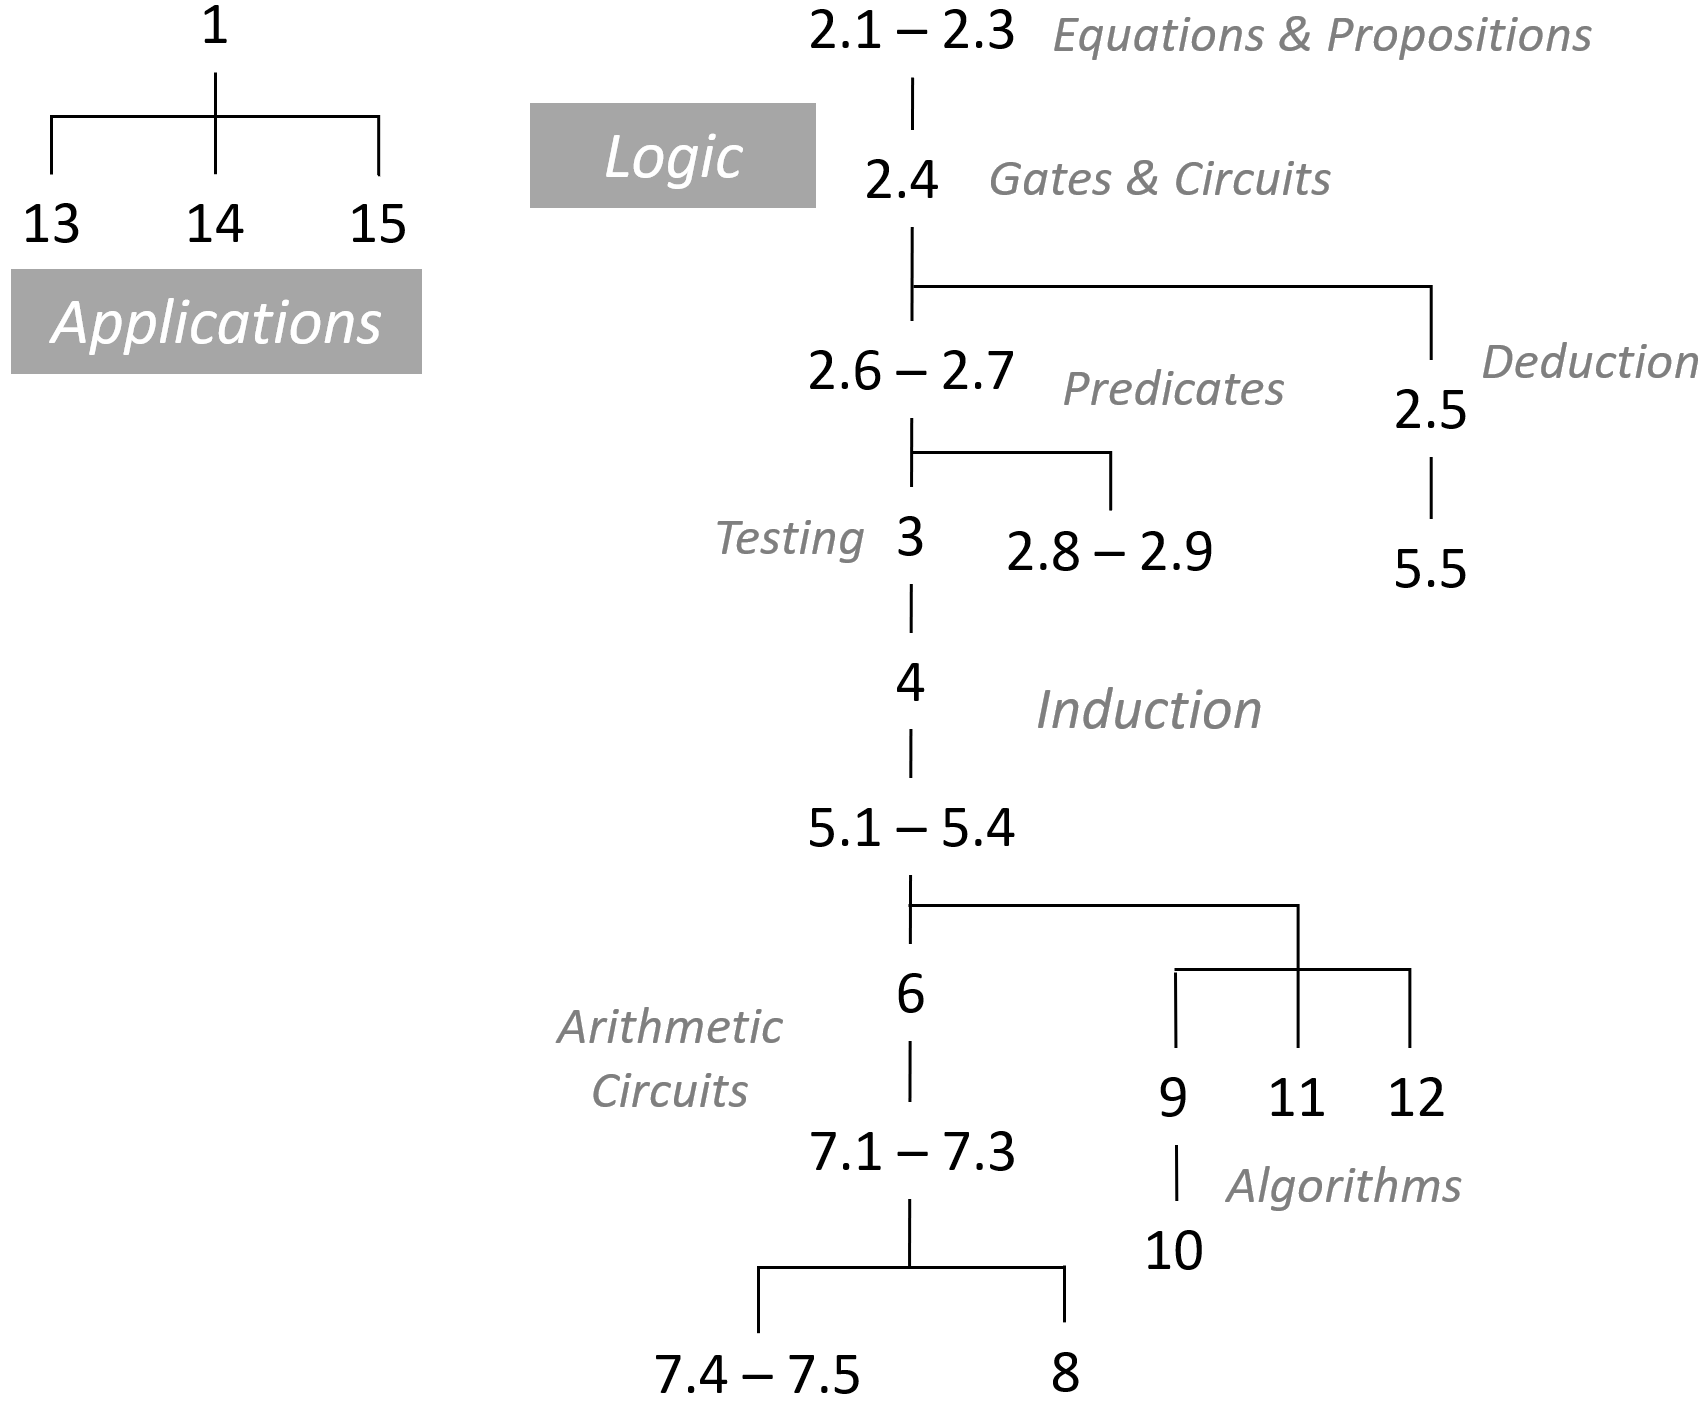
\includegraphics[scale=0.25]{images/roadmap.png}
\end{center}


%%% Local Variables:
%%% mode: latex
%%% TeX-master: "book"
%%% End:


% list of figures
\clearpage
\listoffigures

%list of asides
\clearpage
\listofasides

%preface
\clearpage
\chapter{Preface}
\label{ch:Preface}

Computers are logic in action. Literally.
Many computer components are realizations of formulas in logic,
and when activated by Boolean signals, those components
compute the value of the logic formula that they actualize.
Software, too, is an exhibit in logic.
A software component is a specification in a formal language
with underpinnings in logic,
and in some programming languages a software component
is, literally, an algebraic formula.
A big formula, but a formula nevertheless.

Therefore, people studying computer science
can derive substantial benefit from a study of logic,
and it is perhaps for that reason most computer science students
are exposed to logic during their education.
In many cases, maybe most cases, this exposure comes
in the form of a few lectures and a problem set or two
in a discrete math course. The applications of logic that
they see usually have more to do with traditional mathematics
than with computer science. Even when the discrete math course
is ``discrete math for computer science,'' the computer science
part often has more to do with writing programs to solve problems
in traditional mathematics or to compute examples of
mathematical objects than it has to do with
concepts in computer science.
We think computer science students will
benefit from a substantially more extensive and rigorous
exposure to logic and to seeing many applications of
logic in their chosen field of study.
All the examples in this text arise from issues in computer science.

This book focusses directly on central issues
in computer science.
It frames the discussion in terms of logic,
and it applies logic to problems in the domain of computer science.
Hardware components, software components,
testing and verification, and analysis of algorithms
are some examples.
Instead of illustrating mathematical induction by proving
that a formula represents the sum of a sequence of numbers,
we begin with an inductive proof of an important property of
a software component that concatenates lists,
and we proceed to verify properties of
many other software and hardware components.
It's the same old mathematical induction, but presented
in the context of topics that interest
students of computer science.
The logic of induction is at the forefront,
unobscured by the clever tricks of numeric algebra
that many exercises on induction require in
discussions of the idea that are grounded in topics
of particular interest to mathematicians.

We hope that readers will be inclined
to devote a substantial effort, on the order
of what it takes to absorb a few dozen fifty-minute
lectures at the college level,
to understand some important problems in computer science and
to pursue solutions to many of those problems through formal reasoning.
Formalism is a watchword in this presentation, even to the
point of using the mechanized logic of a partially automated proof engine,
ACL2, that checks proofs to the last detail and can sometimes 
bridge, on its own, gaps that mathematical
proofs often leave open, even when they employ traditional
mathematical rigor.

We chose ACL2 as the proof engine for this work
because in our judgment it provides a more accessible
introduction to mechanized formalism than any other
available proof engine. We do not anticipate that any
reader will become an accomplished ACL2 user,
much less an ACL2 expert. We bring ACL2 into the discussion
to show how logic, including mechanized logic,
can benefit practicing software and hardware engineers.
If at some point readers want to realize those benefits in
large-scale projects, they will need to learn a lot more
about ACL2 or some other mechanized logic than it will
be possible to glean from this introduction.
In early classroom usage of this material,
we introduced formal methods using a traditional algebraic notation,
without a mechanized logic, but most students seem more comfortable
when formal methods are backed up by software tools
that check proofs and provide some aid with proof details.

Logic is the central topic of the text, but not the only topic.
Readers interested in the broad outlines of computer science
will find material useful in that pursuit.
We think the text can provide a basis for a serious introduction
to computer science concepts, both for computer science students
and for students in other fields who want to know
what computer science is about.
Earlier versions of the text have been used many times,
both by the authors and by other instructors,
as the primary text in two types of courses: logic for computer science
and introduction to computer science for both computer science students
and students in other disciplines. It has been used as a supplementary
text in discrete math courses for computer science students.
The text has served well in all three realms.

There are no prerequisites beyond college prep high-school math.
Even less, really.
High-school algebra is helpful,
but no geometry, trigonometry, or calculus is needed.
Computer programming is not a prerequisite, either.
It rarely includes the equation-based model of computation
that informs this presentation and that can
help level the playing ground between people
with programming experience and those without it.

The required learning is far from easy.
Successful students will have to do a lot of hard thinking
to work their way through a few dozen of the exercises,
and they will surely need to do a few dozen exercises to grasp the concepts.
Reading alone won't be enough.
Well over 150 exercises in the text afford students with plenty of opportunities
for problem solving.
Fortunately, the work pays off, both in terms of immediate satisfaction
and in the long term, if the testimonies of former students are a
reliable measure.
We hope readers will take some pleasure in working their way through
the book, and that they will find what they learn
edifying as they go on to other projects.
\\
\\
\emph{Santa Cruz, California}   \hfill Rex Page \\
\emph{Laramie, Wyoming}         \hfill Ruben Gamboa \\
\emph{January 2018}


%%% Local Variables:
%%% mode: latex
%%% TeX-master: "book"
%%% End:


%acknowledgements
\chapter{Acknowledgements}
\label{ch:Acknowledgements}

The authors would like to thank Caleb Eggensperger for developing
the Proof Pad environment that has eased many students 
through early experiences with mechanized logic. 
Carl Eastland, Dale Vaillancourt, and Matthias Felleisen 
built an ACL2 environment that one of the authors relied on 
for many course offerings and which
included DoubleCheck, the predicate-based, automated testing facility 
based on ideas in QuickCheck, the grandaddy 
of such tools invented by John Hughes and Koen Claessen,
that was later incorporated into Proof Pad. 
We thank them for their pioneering work.
Qi Cheng used prototype versions of the text
in applied logic courses and
suggested improvements that made it a better book.
The authors also want to credit the students, 
numbering more than a thousand,
who applied themselves to early versions of the
text and provided their feedback. Thank you, every one.

%%% Local Variables:
%%% mode: latex
%%% TeX-master: "book"
%%% End:


\mainmatter

\raggedbottom

\part{Logic and Equations}

\chapter{Computer Systems: Complex Behavior from Simple Principles}

Computer systems, both hardware and software, are some of the
most complicated artifacts that humans have ever created. But at
their very core, computer systems are straightforward
applications of the same logical principles that philosophers
have been developing for more than two thousand years, and
this book will show you how.

The hardware component of a computer system is made up of the visible
pieces of equipment that you are familiar with, such as monitors,
keyboards, printers, web cameras, and USB storage devices.  It also
includes the 
components inside the computer, such as chips, cables, hard
drives, DVD drives, and boards. 
The properties of hardware devices are largely fixed when the system is
constructed. For example, a hard drive can store 2 gigabytes,
or a cable may be able to transmit 25 different signals
simultaneously---but no more. 

The hardware that makes up a computer system is not much different
than the electronics inside a television set or DVD
player. But computer hardware can do something that other
consumer electronic devices cannot; it can respond to 
information encoded in a special way, what is 
referred to as the software component of the system.  We usually
call the software a ``program.''

You may have heard
about different computer chips and their instruction sets, such
as the Intel chips that power the laptop we are using to
write this book.  Software for these chips consists of a list of
instructions, and that is the way that most general-purpose computer
systems in use today represent software.
But there is nothing magical about this way of thinking about
software; in fact, we believe that thinking about software in this 
way obscures its important features.  For example, during the 1980s
and 1990s, special computers were created that used mathematical
functions as the basis for the software.  And other computer
systems have completely different representations for software.
The Internet service Second Life, for example, can be programmed 
using Scratch for Second Life (S4SL), and programs in S4SL look
like drawings, not instructions.  An even more graphical view of
software is provided by LabView, which is used by scientists and
engineers all over the world to control laboratory equipment.
If you are at a university, there is a good chance
that LabView is being used at one of the laboratories near you!
And software in LabView looks like a large engineering drawing.
In this book, we think of software as consisting of mathematical
formulas.  This view is entirely consistent with the view of
software as a list of instructions or a specialized drawing.  More
important, it makes computer software accessible to anyone with a 
knowledge of high school algebra.

\begin{aside}
Logicians and mathematicians have been studying models of computation
since before computers were invented. This was done, in part, to
answer a deep mathematical question: What parts of mathematics can,
in principle, be fully automated?  In particular, is it possible to
build a machine that can discover all mathematical truths?

As a result, many different models of computation were developed,
including Turing machines, Lambda calculus, partial recursive
functions, unrestricted grammars, Post production rules, ramdom-access
machines, and many others.  Historically, computer science theory has
treated Turing machines as the canonical foundation for computation,
although modern computers are more closely described by the
random-access model.  Our equational model of computation is closely
related to the Lambda calculus.

What is truly remarkable is that all of these different models of 
computation have been shown to be equivalent.  That is,
if a computation can be described in one of these models, it can also
be described in any of the other models.  It is natural, therefore to
extend this observation by conjecturing that all ``reasonable'' models
of computation are equivalent.  This conjecture is called the
Church-Turing Thesis, and it lies at the heart of computer science
theory.

Also remarkable is that some problems cannot be solved by a program
written in any of these computational models.  Of course, since the
models of computation are equivalent, if a problem cannot by solved by
one of the models, it cannot be solved in any of the models.  Alan
Turing, who many consider to be the first theoretical computer
scientist, was the first to discover such uncomputable problems,
shortly after the logician Kurt G\"odel showed that no formal system
of logic could prove all mathematical truths.  Turing's and G\"odel's 
discoveries of uncomputability and incompleteness show that it is
not possible to build a machine that can discover all mathematical
truths, not even in principle.

\caption{Models of Computation}
\label{aside-model-of-computation}
\end{aside}

It is the software that gives a computer system much of its power and
flexibility. An iPhone, for example, has a screen that
can display 441,600 different pixels arranged in a 960x460
grid, but it is the software that determines whether the
iPhone displays an album cover or a weather update. 
Software makes the hardware more useful by extending the way
it behaves. For instance, a speaker may only be able to produce a
single tone at a time. But the software can instruct the speaker to
play a sequence of tones that sounds like Beethoven's Fifth Symphony.

The mental image you should have is that hardware consists of
the parts in a computer system that you can see, and software
consists of the information that tells the system what to do.
But the distinction between hardware and software is not as
clear cut as this suggests. Many hardware components actually
encode software directly and control other pieces of the system. 
In fact, hardware today is designed and built using many techniques
first developed to build large software projects.  And we will see in
this book that both hardware and software can be modeled using formal
logic.

The distinction between hardware and software is well and good,
but it leaves many questions to the imagination.
At the very least, we must answer the following questions:
\begin{enumerate}
\item How can software affect hardware, e.g., instruct a
        speaker to play a note?
\item How can software detect the hardware’s current status, e.g.,
        whether a switch is pressed or not?
\item What other instructions can the software give the hardware,
        e.g., add two numbers or move data from one location to
        another?
\end{enumerate}

We'll start with the last question.  The answer to this is provided by
a model of computation, as described in Aside~\ref{aside-model-of-computation}.
In fact, there are as many answers to this question as there are
models of computation, and logicians have been very creative when it
comes to constructing such models!  Luckily, these models are
completely equivalent to each other, so we can choose the answer
that is most convenient to us.  And the most convenient answer is 
that a program consists of basic mathematical primitives, such as
the arithmetic functions, and the ability to define new functions.

Once we take functions as the basic model of computation, then the
answers to the other questions are natural.  The software can affect
the hardware by the values that the function returns.  For example,
a program---that is, a function---can tell an iPhone what to display
in its screen by returning a 960x460 matrix.  Each entry in the matrix
can be a number that represents a color, for example 16,711,680 for
red or 65,280 for green.  Similarly, the hardware can inform the
software of its current status via the function's parameters.  For
example, the input to the function can be the coordinates of the pixel
that the user selected by tapping the screen with her finger.  Of
course, the user may perform different gestures, such as tapping or
scrolling.  Each gesture will trigger a different function.

To make this clear, let's consider a simple example.  We will build a
simple computer device that plays rock-paper-scissors.  The machine
has three buttons, allowing the user to select rock, paper, or
scissors.  The device also has a simple display unit.  After the user 
makes a selection, the display unit shows the computer's choice and
lets the user know who won that round.  Our program will make the
selection and determine the winner.  To keep things fair, we will
write this program as two separate functions, so the selection
function cannot ``see'' the user's choice.

The first function, called \texttt{emily}\footnote{This function is
named after one of the authors' children.  The ``real'' Emily
plays rock-paper-scissors game just like the program developed in this
chapter.}, makes the computer's choice.  The output of this function
is obvious: It should be one of ``rock'', ``paper'', or ``scissors''.
If it makes you feel better, you can think of this output as 0, 1, or 2.
But one of the things that makes computers so useful is that they can work
with any type of information, not just numbers.

But what about the input to the function \texttt{emily}?  Remember
that the value of a mathematical function is completely determined by
its inputs.  That's what it means to be a function! So if
\texttt{emily} has no inputs, it must always return the same value,
and that would be a very boring game.  We've already decided that it
would be unfair for \texttt{emily} to see the user's current choice,
but what about the last round?  We can make our selection by
considering the last round of the game, so the input can be the user's
\emph{previous} choice---or a special token, like ``N/A'' for the
game's first round.  The function \texttt{emily} can now be described
as follows:
\begin{displaymath}
emily(u) =
   \left\{
        \begin{array}{ll}
        \mbox{``rock''}     & \mbox{if } u = \mbox{``scissors''} \\
        \mbox{``paper''}    & \mbox{if } u = \mbox{``rock''} \\
        \mbox{``scissors''} & \mbox{otherwise}
        \end{array}     
   \right.
\end{displaymath}       

The second function, which can be called \texttt{score}, decides who
was the winner of the round.  Its input corresponds to the choices
made by the computer and the user, respectively.  Its output consists
of a pair or values.  The first value determines the winner, and the
second ``remembers'' the user's choice.
\begin{displaymath}
score(c,u) =
   \left\{
        \begin{array}{ll}
        (\mbox{``none''}, u)     & \mbox{if } c = u \\
        (\mbox{``computer''}, u) & \mbox{if } (c,u) = (\mbox{``rock''}, \mbox{``scissors''}) \\
        (\mbox{``user''}, u)     & \mbox{if } (c,u) = (\mbox{``rock''}, \mbox{``paper''}) \\
        (\mbox{``computer''}, u) & \mbox{if } (c,u) = (\mbox{``paper''}, \mbox{``rock''}) \\
        (\mbox{``user''}, u)     & \mbox{if } (c,u) = (\mbox{``paper''}, \mbox{``scissors''}) \\
        (\mbox{``computer''}, u) & \mbox{if } (c,u) = (\mbox{``scissors''}, \mbox{``paper''}) \\
        (\mbox{``user''}, u)     & \mbox{if } (c,u) = (\mbox{``scissors''}, \mbox{``rock''})
        \end{array}     
   \right.
\end{displaymath}       
What is the point of the second value of \texttt{score}?  As you can
see, it is always equal to $u$, i.e., the user's selection.  The
intent is that this second returned value will be passed as the input
to the next call of \texttt{emily}.  This is how the program can
remember the user's previous choice.

We could certainly have dropped this second return value, and simply
stipulated that the hardware is responsible for remembering
the user's last selection.  However, we chose to write the program
in this way for two reasons.  First, it gives us more flexibility.
The hardware is simply responsible for storing the value returned 
by \texttt{score} and sending it to \texttt{emily} in the next round.
We can make the program a more sophisticated player of
rock-paper-scissors by changing the software, possibly changing the
value that is passed from \texttt{score} to \texttt{emily} in the
process.  For example, a more sophisticated program may want to
keep track of the number of times that the user has selected each of
the choices.  Since it's the software that decides what to remember
from each round, this choice can be changed very easily.  That is
the flexibility and power of software.

The second reason for writing the program in this way is that it
gives us an opportunity to make an important point about our
computational model.  Since our programs are written as mathematical
functions, they cannot ``remember'' anything.  Programmers who are
used to other computational models (such as C++ or Java) may be
very surprised by this!  It is natural in those models to store
values in ``variables'' and use those variables later in the program,
but that is not possible in our purely functional model.  However, our
model allows the \emph{hardware} to keep certain values, in much the
same way that the hardware can tell which button was pressed by the
user.  In fact, each button ``remembers'' whether it's pressed or not.
Our model of computation simply allows the hardware to have some
``hidden'' buttons that can store information and later pass it to
another function.

This model is very simple, and you could be forgiven for thinking that
there has to more to it, that computers must be much more complicated.
But in fact, that's all there is.  Consider \textit{Deep Blue}, the
computer that beat world champion Gary Kasparov at chess on May 11,
1997.  This program can be written as a function with a single input,
an 8x8 matrix of numbers that represent the position of the pieces
on the board after Kasparov's last move.  The function's output is 
either the position of the board after its move, or a special
white-flag token used to ``resign'' the game.

In principle, a chess-playing function can be written as follows.
Given the input board, determine all possible legal moves.  If there
are no legal moves, resign.  If there is a legal move that results
in checkmate, do that move.  Otherwise, for each legal move, consider
each of the possible moves by the opponent.  Each one of those results
in a new board, which can then be examined by our chess-playing
function!  It may seem surprising that a function can be defined this
way, but such ``recursive'' functions are common in mathematics, the
most common being the factorial function, defined by the equation 
\begin{displaymath}
n! = 
\left\{
        \begin{array}{ll}
                1              & \mbox{if } n = 0 \\
                n \cdot (n-1)! & \mbox{otherwise}
        \end{array}     
\right.
\end{displaymath}       
We will use recursive functions extensively in the rest of this book.

The problem with this naive chess-playing function is that there are
too many moves to consider.  While the function can, \emph{in principle},
select the best move to play next, \emph{in practice}, the computation
would take too much time---more than the expected lifetime of the
universe with current technology.  But in fact, \textit{Deep Blue}
did play like this, only it used a massively parallel computer so that
it could consider many moves at the same time, and in most cases it
considered only six to eight moves in the future.  In practice,
\textit{Deep Blue} is a complicated function, with a large
definition.  But in principle, it is just a mathematical function,
just like the programs we will study in this book. 

\begin{ExerciseList}
\Exercise This is the first exercise
        \Question what do you think?
        \Question are you sure?

\Exercise Another exercise
        \Question really?
\end{ExerciseList}      
        
%%% Local Variables: 
%%% mode: latex
%%% TeX-master: "book"
%%% End: 


\chapter{Boolean Formulas and Equations}
\label{ch:Boolean-Formulas}

\section{Reasoning with Equations}
\label{sec:math-and-equations}
\index{symbolic logic}\index{logic!symbolic}Symbolic logic,
like other parts of mathematics, starts from a small
collection of axioms and employs rules of inference to find
additional propositions consistent with those axioms. This
chapter will define a grammar of logic formulas, postulate a few
equations stating that certain formulas carry the same meaning as others,
and derive new equations
using substitution of equals for equals as the rule of
inference.

You will probably find this familiar from your
experience with numeric algebra, but the discourse here will attend carefully
to details, and this formality may extend beyond what you are
accustomed to. What it buys is mechanization. That is,
logic formulas and reasoning about them will amount to
mechanized computation, and this will make it possible for
computers to check that our reasoning follows all the rules,
without exception. This justifies more confidence
in conclusions than would otherwise be possible.

We will be doing all of this in the domain of symbolic logic, which
includes operations like ``logical or'' and ``logical negation,''
rather than arithmetic operations, such as addition and
multiplication.
We will be doing Boolean algebra rather than numeric algebra,
but the underlying rule of inference, namely,
substitution\index{reasoning!with equations}\index{substitution}\index{formula!substitution}
of equals for equals,
applies equally well to both Boolean and numeric formulas.
To illustrate the level of formality that we are shooting for,
let's see how it works with a problem
in the familiar domain of numeric algebra.

You are surely familiar with the equation $(-1) \times (-1) = 1$, but you may
not know that it is a consequence of some basic facts about
arithmetic.
That is, the fact that multiplying two
negative numbers produces a positive one
is not independent of other facts about numbers,
and it is not an arbitrary decision either.
Instead, it is an inference one can draw
from an acceptance of other familiar equations.
We will derive the equation $(-1)\times(-1) = 1$
from equations that you have accepted without question for a long time.

The equations in figure~\ref{fig-02-01} (page \pageref{fig-02-01})
express some standard rules of numeric computation.
In those equations, the letters stand in
place of numbers. They can also stand in place of other
formulas.
So, the variable $x$ stands for a grammatically correct formula,
which could be something simple, such as $2$, or
it could be a more complicated formula, such as $3 \times (y + 1)$.

We refer to letters used in this way as
\index{variable}variables, even though within a particular equation they
stand for a fixed number or a particular formula.
The formula associated with a variable, although unspecified,
is the same for every occurrence of the variable in the equation.
If $x$ stands for $3\times(y + 1)$ at one point in the
equation, then everywhere else $x$ occurs in the equation,
it stands for that same formula, $3\times(y + 1)$.
This is the usual custom in algebra.

\begin{aside}{aside-hold-on-to-seat}{Hold on to Your Seat}
Mathematical formulas communicate
information using a formal grammar imbued with specific meanings.
The grammar determines which phrases are well formed
and which are not.
For example, $x+3\times(y + z)$ conforms to a grammar
of numeric formulas.
It is grammatically correct, and it stands for a
particular and carefully prescribed calculation.
The nonformula $x+3 \times (y + ) \times z$
does not conform to that grammar and therefore
carries no meaning.
Reasoning about computer hardware and software
calls for a high degree of \index{formalism}formality to ensure
a level of consistency that is essential to  its usefulness.

Rigorous formality takes many readers by surprise.
It takes some getting used to.
Things may seem overly simple in the beginning.
Then, suddenly, you may find yourself thrashing around in deep water.
Take a deep breath and slowly work  through the material.
It provides a basis for everything to follow.
The ideas and methods call for careful study and frequent review.
When things start to go off track,
slow down, back up a little, and try
again.\index{panic, don't}\index{disheartened?}\index{frustrated?}\index{baffled?}\index{worried?}\index{scared?}\index{funk, in a?}
Gradually, the pieces will fall into place,
but you can expect to run into some bumps.
\emph{Hold on to your seat.}
%\caption{Hold on to Your Seat}
%\label{aside-hold-on-to-seat}\index{seat, hold on}\index{hold onto your seat}
\end{aside}

\begin{figure}
\begin{center}
\begin{spacing}{0.9}
\begin{tabular}{ll}
$x+0 = x$                 & \{$+$ identity\} \\
$(-x)+ x = 0$             & \{$+$ complement\} \\
$x \times 1 = x$          & \{$\times$ identity\} \\
$x \times 0 = 0$          & \{$\times$ null\} \\
$x+y = y+x$               & \{$+$ commutative\} \\
$x \times y = y \times x$ & \{$\times$ commutative\} \\
$x+(y+z) = (x+y)+z$       & \{$+$ associative\} \\
$x \times (y \times z) = (x \times y) \times z$ & \{$\times$ associative\} \\
$x\times(y+z) = (x \times y)+(x \times z)$      & \{distributive law\} \\
\end{tabular}
\end{spacing}
\end{center}\index{equation, by name!\{$+$ identity\}}\index{equation, by name!\{$+$ complement\}}\index{equation, by name!\{$\times$ identity\}}\index{equation, by name!\{$\times$ null\}}\index{equation, by name!\{$+$ commutative\}}\index{equation, by name!\{$\times$ commutative\}}\index{equation, by name!\{$+$ associative\}}\index{equation!numeric algebra}\index{axiom!numeric algebra}\index{reasoning!with equations}
\caption{Equations of numeric algebra.}
\label{fig-02-01}
\end{figure}

If we accept the equations of figure~\ref{fig-02-01},
we can apply one of them to transform the formula $(-1)\times(-1)$ to a new formula that
stands for the same number. Then, we can apply another equation to
transform that formula to a new one, and so on.
We look for a way to apply the
accepted equations one by one, so that in the end we
arrive at the formula $1$. At every step, we know that the
new formula stands for the same number as the old one, so in
the end we know that $(-1)\times(-1) = 1$.

Figure~\ref{fig-02-02} (page \pageref{fig-02-02})
displays this sort of equation-by-equation derivation of the
formula $1$ from the formula $(-1)\times(-1)$. To
understand figure~\ref{fig-02-02}, you must remember that each
variable can denote any
grammatically correct formula. For example, in the
equation $x + 0 = x$,
which is called the \{$+$ identity\} equation,
the variable $x$ could stand for a number,
such as 3, or it could stand for a more complicated
formula, such as $(1 + 3)$. It could even stand for a formula
with variables in it, such as $(a + (b \times c))$ or
$(((-1) \times (x + 3)) + (x + y))$.

Another crucial point is that each step cites
exactly one equation from figure~\ref{fig-02-01}
to justify the transformation from the formula in the previous step.
We are so accustomed to calculating with numeric formulas that
we often combine many basic steps into one. When we reason formally,
we are careful to do just one step at a time.
We justify each step by citing an equation
from a list of known equations. In our proof of $(-1)\times(-1) = 1$,
we will justify steps by citing equations from figure~\ref{fig-02-01}
and from no other source. We will not skip steps.
Keep that in mind as you go through the proof, line by line.

The first step in the proof
(figure~\ref{fig-02-02}, page \pageref{fig-02-02}) uses a version of the
\{$+$ identity\} equation in which the variable $x$ stands for the
formula $((-1)\times(-1))$.
In this context, the \{$+$ identity\} equation
leads to the new formula $((-1)\times(-1)) + 0$.

The second step in the proof reads the \{$+$ complement\}
equation backwards (equations go both ways) and in a form
where the variable $x$ stands for the number 1.
When $x$ is 1, the \{$+$ complement\} equation is
$(-1) + 1 = 0$.
Reading the equation backwards, we can substitute
$((-1) + 1)$ for $0$,
and that leads to the formula $((-1)\times(-1)) + ((-1) + 1)$.
So, we know now that
$(-1)\times(-1) = ((-1)\times(-1)) + ((-1) + 1)$.

Doesn't really seem like progress does it?
But, we press on anyway, one step at a time.
The transformations, step by step, finally confirm that the two formulas
$(-1)\times(-1)$ and 1 represent the same number.

Pay particular attention to the last three lines of the proof.
Most people tend to jump from the formula $0+1$ to the
formula $1$ in one step. That jump requires knowing the equation
$0+1 = 1$. However, that equation is not among those listed in
figure~\ref{fig-02-01}.
We want to do the proof without citing any equations
other than those in figure~\ref{fig-02-01}, so we need two steps
to get from $(0+1)$ to $1$,
and those are the last two steps in the proof.

\begin{figure}
\begin{center}
\begin{spacing}{0.9}
\begin{tabular}{lll}
    & $(-1)\times(-1)$                            & \\
$=$ & $((-1)\times(-1)) + 0$                      & \{$+$ identity\} \\
$=$ & $((-1)\times(-1)) + ((-1) + 1)$             & \{$+$ complement\} \\
$=$ & $(((-1)\times(-1)) + (-1)) + 1$             & \{$+$ associative\} \\
$=$ & $(((-1)\times(-1)) + ((-1) \times 1)) + 1$  & \{$\times$ identity\} \\
$=$ & $((-1)\times((-1) + 1)) + 1$                & \{distributive law\} \\
$=$ & $((-1)\times 0) + 1$                        & \{$+$ complement\} \\
$=$ & $0 + 1$                                     & \{$\times$ null\} \\
$=$ & $1 + 0$                                     & \{$+$ commutative\} \\
$=$ & $1$                                         & \{$+$ identity\} \\
\end{tabular}
\end{spacing}
\end{center}\index{negative $\times$ negative}\index{equation!proof by}\index{proof!with equations}\index{commutative}\index{distributive}\index{reasoning!with equations}\index{equation!citation}\index{citation!equation}
\caption{Why $(-1)\times(-1)=1$.}
\label{fig-02-02}
\end{figure}

One of the things we hope you will glean from this derivation is that
the equation $(-1)\times(-1) = 1$ does not depend on vague,
philosophical assertions like ``two negatives make a positive.''
Instead, the equation $(-1)\times(-1) = 1$ is a consequence of some
basic arithmetic equations. If you accept the basic equations
and the idea of substituting equals for equals,\footnote{Substituting
equals for equals applies the first of
\index{Euclid}Euclid's \index{common notions}common notions:
Things which are equal to the same thing are also equal to one another.
%Failed attempt to quote Euclid in Greek ... probably bad idea anyway
%(Or, ``\textgreek{Ηἰτήσθω ἀπὸ παντὸς σημείου ἐπὶ πᾶν σημεῖον εὐθεῖαν γραμμὴν ἀγαγεῖν}'',
%as Euclid may have put it.)
People have been reasoning by substitution for a long time.}
you must, as a rational consequence, accept the equation
$(-1)\times(-1) = 1$.

Using this same kind of reasoning, we will derive new Boolean equations
from a few basic ones postulated as axioms.
A Boolean \emph{axiom} is a Boolean equation
that we assume to be true, without proof.
We will also learn that digital circuits are physical
manifestations of logic formulas, and we will be able to
parlay that idea to derive behavioral properties of
computer components.

Likewise, because a computer program is,
literally, a formula, we will be able to derive
properties of software directly from the programs themselves.
This makes it possible for us to be entirely
certain about some of the behavioral characteristics of
software and of the digital circuits that
comprise hardware components.
Our certainty stems from the mechanistic
\index{formalism}formalism that we insist on from the beginning,
which can be checked to the last detail with automated computation.

\begin{exercises}
\label{ex:ch02-intro}
\exer {Use the equations of figure~\ref{fig-02-01} (page \pageref{fig-02-01}),
together with the additional equation $(1 + 1) = 2$, to derive the equation $(x + x) = (2 \times x)$.}

\exer {\label{ex:times-negation}%
Derive the following equation
using using the equations of figure~\ref{fig-02-01}:
\begin{center}
$((-1) \times x) + x = 0$ ~~~~~ \{$\times$ negation\}
\end{center}}

\exer {Derive the equation $((x + (((-1) \times (x + y)) + z)) + y) = z$
using using the equations of figure~\ref{fig-02-01} and,
if you like,
the \{$\times$ negation\} equation from exercise \ref{ex:times-negation}.}
\end{exercises}

\section{Boolean equations}
\label{sec:boolean-equations}
Let's start with the Boolean equations in
figure~\ref{fig-02-03} (page \pageref{fig-02-03}).
These equations, which we will call the
\index{Boolean!axiom}Boolean \index{axiom!Boolean algebra}axioms,
are the starting point for our system of reasoning.
They form the basis from which we will derive
a host of other equations.
If these axiomatic \index{equation!as axiom}equations
are new to you and seem strange,
try to view them as ordinary
algebraic equations, but with a different collection of operators.
A formula in numeric algebra has operations like addition
($+$) and multiplication ($\times$). Boolean formulas employ logic
operations: logical-and ($\wedge$), logical-or ($\vee$),
logical-negation ($\neg$), and implication ($\rightarrow$).
Furthermore, Boolean formulas stand for logic values
($True$, $False$), rather than for numbers ($\dots$ $-2$, $-1$, $0$, $1$, $2$ $\dots$).

\begin{figure}
\begin{center}
\begin{spacing}{0.9}
\begin{tabular}{ll}
$x \vee False = x$                                   & \{$\vee$ identity\} \\
$x \vee True = True$                                 & \{$\vee$ null\} \\
$x \vee y = y \vee x$                                & \{$\vee$ commutative\} \\
$x \vee (y \vee z) = (x \vee y) \vee z$              & \{$\vee$ associative\} \\
$x \vee (y \wedge z) = (x \vee y) \wedge (x \vee z)$ & \{$\vee$ distributive\} \\
$x \rightarrow y = (\neg x) \vee y$                  & \{implication\} \\
$\neg(x \vee y) = (\neg x) \wedge (\neg y)$          & \{$\vee$ DeMorgan\} \\
$x \vee x = x$                                       & \{$\vee$ idempotent\} \\
$x \rightarrow x = True$                             & \{self-implication\} \\
$\neg(\neg x)  = x$                                  & \{double negation\} \\
\end{tabular}
\end{spacing}
\end{center}\index{Boolean!algebra}\index{commutative}\index{distributive}\seeonlyindex{algebra, Boolean}{Boolean, algebra}\index{reasoning!with equations}\index{axiom!commutative}\index{axiom!associative}\index{axiom!parentheses}\index{axiom!Boolean algebra}\index{axiom, by name!\{$\vee$ identity\}}\index{axiom, by name!\{$\vee$ null\}}\index{axiom, by name!\{$\vee$ commutative\}}\index{axiom, by name!\{$\vee$ associative\}}\index{axiom, by name!\{$\vee$ distributive\}}\index{axiom, by name!\{implication\}}\index{axiom, by name!\{$\vee$ DeMorgan\}}\index{axiom!DeMorgan}\index{axiom, by name!\{$\vee$ idempotent\}}\index{axiom!idempotent}\index{axiom, by name!\{self-implication\}}\index{axiom, by name!\{double negation\}}\index{axiom, by name!\{atomic release\}}\index{equation!grammar}\index{equation!distributive}\index{equation!Boolean algebra}\index{equation!commutative}\index{equation!associative}\index{equation!parentheses}\index{equation!Boolean algebra}\index{equation, by name!\{$\vee$ identity\}}\index{equation, by name!\{$\vee$ null\}}\index{equation, by name!\{$\vee$ commutative\}}\index{equation, by name!\{$\vee$ associative\}}\index{equation, by name!\{$\vee$ distributive\}}\index{equation, by name!\{implication\}}\index{equation, by name!\{$\vee$ DeMorgan\}}\index{equation!DeMorgan}\index{equation, by name!\{$\vee$ idempotent\}}\index{equation, by name!\{idempotent\}}\index{equation, by name!\{self-implication\}}\index{equation, by name!\{double negation\}}\index{operator, logic!and ($\wedge$)}\index{operator, logic!or ($\vee$)}\index{operator, logic!not ($\neg$)}\index{operator, logic!implication ($\rightarrow$)}\seeonlyindex{logic operator}{operator, logic}
\caption{Boolean axioms (basic equations).}
\label{fig-02-03}
\end{figure}

When we derive a new equation by citing an equation that was
itself derived rather than by citing an axiomatic equation
from figure~\ref{fig-02-03},
we refer to the cited equation as a \index{theorem}\emph{theorem} to
distinguish it from an axiom.
The new \index{equation!as theorem}equation is also a theorem,
and it can be cited in \index{derivation}derivations of other new equations.
We call such a derivation of a new equation a
\index{proof}\emph{proof} of the equation.

\begin{figure}
\begin{theorem}[\{$\vee$ truth table\}]
\mbox{}
\begin{itemize}
\item $False \vee False = False$
\item $False \vee True  = True$
\item $True  \vee False = True$
\item $True  \vee True  = True$
\end{itemize}
\end{theorem}

\begin{proof}
\mbox{}\\
\begin{tabular}{llll}
    &$False \vee False$    & \\
$=$ & $False$              & \{$\vee$ identity\}  &---replace $x$ in the axiom with \emph{False}\\
    &  ~                   & \\
    & $False \vee True$    & \\
$=$ & $True$               & \{$\vee$ null\}      &---replace $x$ in the axiom with \emph{False}\\
%    &                      & \dots for practice, prove the other two equations yourself \dots \\
\end{tabular}
\begin{quote}
\dots for practice, prove the other two equations yourself \dots
\end{quote}
\end{proof}
\index{equation!proof by}
\index{proof!with equations}
\index{truth table}
\caption{Proof of theorem \{$\vee$ truth table\}.}
\label{or-truth-table}
\end{figure}

The first equation in the theorem \{$\vee$ truth table\}
(figure~\ref{or-truth-table}, page \pageref{or-truth-table})
is a special case of the
\{$\vee$ identity\} axiom (figure~\ref{fig-02-03}),
and the proof of that equation simply amounts making that observation.
That is, the proof just rewrites the \{$\vee$ identity\} axiom
with $False$ in place of $x$.
The proof of the second equation is equally short, but it cites
a different axiom.
For practice, try to prove the other two
equations in the \{$\vee$ truth table\} theorem
by citing axioms in a similar way.

We are serious about that. Did you prove the other two equations?
No? Well \dots go back and do it, then. Without participation, there
is no learning. $\dots$ \emph{We'll wait here}$\dots$

Finished now? Good for you. You cited the \{$\vee$ identity\} axiom in your
proof of the third equation in the theorem and the \{$\vee$ null\}
axiom in your proof of the fourth equation, right? We knew you could do it.

\begin{aside}{truth-tables}{Truth Tables}
A \emph{truth table} for a formula is a list of equations
stating the values that the formula represents.
There is one equation in the truth table for each possible
combination of values for the variables in the formula.
If there is only one variable in the formula,
there will be two equations in its truth table,
one for the case when the variable has the value
$True$ and one for the case when it has the value $False$.
If there are two variables in the formula,
there will be four equations in the truth table
because for each choice of value for the first variable,
there are two choices for the other.
Three variables lead to eight equations.
The number of equations in the truth table
doubles with each additional variable
in the formula.

A truth table for a logic operator is the truth table for the formula
that has variables in place of the operands.
For example, the truth table for the logical-or operator ($\vee$)
is the truth table for the formula $(x \vee y)$.
That formula has two variables, so the truth table has four equations.
%\caption{Truth Tables}
%\label{truth-tables}
\end{aside}

Derivations are usually more than one step, of course.
The \{$\vee$ complement\} theorem
(figure~\ref{fig:or-complement-thm}, page \pageref{fig:or-complement-thm})
has a two-step proof, citing the \{implication\} axiom
and the \{self-implication\} axiom.
The \{$\vee$ complement\} theorem is often called the
\index{law of the excluded middle}``law of the excluded middle''
because it says that any logic formula,
together with its negation, covers all of the possibilities.
A formula in logic is either true or false.
There is no middle ground.

\begin{figure}
\begin{theorem}[\{$\vee$ complement\}]
$(\neg x) \vee x = True$
\end{theorem}
\begin{proof}
\mbox{}\\
\begin{tabular}{lll}
    & $(\neg x) \vee x$ & \\
$=$ & $x \rightarrow x$ & \{implication\} \\
$=$ & $True$            & \{self-implication\} \\
\end{tabular}

\end{proof}
\index{equation!proof by}
\index{proof!with equations}
\index{equation, by name!\{$\vee$ complement\}}
\index{excluded middle}
\index{equation!excluded middle}
\index{law of the excluded middle}
\caption{Proof of theorem \{$\vee$ complement\}.}
\label{fig:or-complement-thm}
\end{figure}

All of the logic operators have truth tables,
and we can derive the equations in those truth tables from the axioms.
Figure~\ref{fig:neg-truth-table} (page \pageref{fig:neg-truth-table})
displays the truth table
for the negation operator $(\neg)$.
The figure includes a four-step proof of the first equation in
the table.
To beef up your comprehension of the ideas,
construct your own proof of the second equation in the theorem.

\begin{figure}
\begin{theorem}[\{$\neg$ truth table\}]
\mbox{}\\
\begin{itemize}
\item $\neg True = False$
\item $\neg False = True$
\end{itemize}
\end{theorem}
\begin{proof}
\mbox{} \\
\begin{tabular}{llll}
    & $\neg True$                      & \\
$=$ & $\neg (False \rightarrow False)$ & \{self-implication\} \\
$=$ & $\neg ((\neg False) \vee False)$ & \{implication\}     &---replace $x$ and $y$ in axiom with $False$ \\
$=$ & $\neg (\neg False)$              & \{$\vee$ identity\} &---replace $x$ in the axiom with $\neg False$ \\
$=$ & $False$                          & \{double negation\} &---replace $x$ in axiom with $False$ \\
\end{tabular}

\bigskip
\noindent
\begin{tabular}{lll}
    & $\neg False$                             & \\
$=$ & \dots you fill in the details here \dots & \\
$=$ & $True$                                   & \\
\end{tabular}

\end{proof}
\index{equation!proof by}
\index{proof!with equations}
\index{truth table}
\caption{Proof of theorem \{$\neg$ truth table\}.}
\label{fig:neg-truth-table}
\end{figure}

An important facet of these proofs is that they are
entirely syntactic. That is, they apply axioms by
matching the grammar of a formula $f$ (or a subformula of $f$) in the proof
with a formula $g$ from one side of an equation in the axioms.
The matching associates the variables in $g$ with corresponding subformulas of $f$.
Then, the formula $h$ on the other side of
the axiomatic equation is rewritten,
replacing each variable in $h$ with the subformula of $f$
that the matching process established.
The rewritten version of $h$
becomes the new, derived formula.
We know that the derived formula stands for the same value
as the original formula because the axiom asserts this equivalence,
and we assume the axioms are right.

\begin{aside}{feasibility}{Truth Tables and Feasibility}
Reasoning from equations is one way to prove that two formulas stand
for the same value.
Another way is to build truth tables for both formulas.
If the tables match, value for value, you can conclude that
the formulas are equal.
When there are only a few variables and therefore only a few combinations,
the truth tables can be compared quickly and accurately.
Unfortunately, this approach quickly goes south when there are many variables.
With two variables, as in the truth table
for logical-or, there are four combinations of values
(two choices for each variable, $True$ or $False$, so two times two
combinations in all). With three variables, there are eight
($2^3$) combinations, which makes the truth-table method tedious
but not infeasible.

With ten variables, there are 1,024 ($2^{10}$) combinations,
and with twenty, over a million.
Too much for people to handle but easy for computers.
However, a formula specifying a computing component,
hardware or software, has hundreds of variables.
We want to reason about computing components,
and there is no hope of doing that with truth tables.
With a hundred variables, there are $2^{100}$ combinations,
and that number is so large that no computer could
finish checking all the cases before the sun runs out of fuel.
Truth tables are infeasible in this realm.

Proofs like those that make up the core of this book
are not the only effective way to work with large formulas.
Hardware and software designers sometimes use
SMT solvers (satisfiability modulo theories),
BDD tools (binary decision diagrams), or other similar methods
to verify properties of circuits and computer programs,
but such tools don't apply to all formulas.
Reasoning based on grammatical form
makes it feasible to deal with any logic formula,
regardless of the number of variables,
because the formulas can be split into parts small enough
to manage, and those parts can be reintegrated, based on
their grammatical relationships, to produce a full analysis.
Feasible doesn't mean easy, though.
It takes a lot of effort, but it can pay off.\index{truth table}\index{feasibility}\index{infeasibility}
%\caption{Truth Tables and Feasibility}
%\label{feasibility}
\end{aside}

Let's prove another truth-table theorem, partly to practice
reasoning with equations but also to discuss a common
point of confusion about logic. The implication operator
($\rightarrow$) is a cornerstone of logic in real-world problems,
but it is common to get tripped up when it comes to
reasoning with implication.

The \{$\rightarrow$ truth table\} theorem
(figure~\ref{implication-truth-table}, page \pageref{implication-truth-table})
provides the truth table
for the implication operator.
An important aspect of the proof is that it cites
not only axioms from figure~\ref{fig-02-03} (page \pageref{fig-02-03})
but also equations from the \{$\neg$ truth table\} theorem.
This is the way mathematics goes. Once we have derived
a new equation from the axioms, we can cite
the new equation to derive still more equations.

\begin{aside}{abstraction}{Abstraction}
Citing proven theorems to prove new ones
is similar to an idea known as
\index{abstraction}abstraction
in engineering design.
Instead of citing an old theorem to prove a new one,
we could copy the proof of the old theorem into the new proof.
However, that would make the proof longer, harder to understand,
and more likely to contain errors.

Computer programs are built from components that are themselves
also computer programs. As components become available,
they are used to build more complex components.
Sometimes, a component has almost the right form
to be used in a new program but not quite.
Maybe the existing component doubles a number,
but the new usage needs to triple it.
It is tempting to copy the
old component, change $2 \times x$ to $3 \times x$,
and paste the revised component into the program.

In our experience, \index{copy-and-paste programming}copy-and-paste
programming is a common source of errors in software,
especially in programs maintained
over time. When a maintainer finds an error in
a component that was copied from elsewhere,
there is nothing to direct the maintainer to fix
the same error in the original component.
A better choice, most of the time,
is to make a new component with
a variable, say $m$, in place of the $2$.
This is known as creating an abstraction of the component
(``abstract'' as opposed to ``specific'' or ``concrete'').

The new component can be used for both doubling and tripling
simply by specifying $2$ for $m$ in one case and $3$ for $m$ in the other.
If later in the project an error is discovered in the component,
the error only needs to be fixed in one place, not two,
or maybe ten or a hundred places, depending on how many engineers
copied the original component to make a change.
Abstraction is an important engineering method.
Citing old theorems to prove new ones has similar advantages.
%\caption{Abstraction}
%\label{abstraction}
\end{aside}

\begin{figure}
\begin{theorem}[\{$\rightarrow$ truth table\}]
\mbox{}
\begin{itemize}
\item $False \rightarrow False = True$
\item $False \rightarrow True  = True$
\item $True  \rightarrow False = False$
\item $True  \rightarrow True  = True$
\end{itemize}
\end{theorem}

\begin{proof}
\mbox{} \\
\begin{tabular}{llll}
    & $False \rightarrow False$        & \\
$=$ & $(\neg False) \vee False$        & \{implication\} &---\emph{put} $False$ \emph{for} $x$ \emph{and for} $y$ \emph{in axiom}\\
$=$ & $\neg False$                     & \{$\vee$ identity\}\\
$=$ & $True$                           & \{$\neg$ truth table\}\\
\end{tabular}

\begin{tabular}{lll}
& \dots for practice, prove the other equations yourself\dots & \\
\end{tabular}

\end{proof}
\caption{Proof of theorem \{$\rightarrow$ truth table\}.}
\index{truth table}
\label{implication-truth-table}
\end{figure}

In day-to-day life outside the domain of symbolic logic,
the usual interpretation of the logical implication $x \rightarrow y$
is to conclude that $y$ is true whenever
$x$ is true. However, the implication says nothing
about $y$ when $x$ is not true. In particular, it
does not say that $y$ is not true when $x$ is not true.
Theorem \{$\rightarrow$ truth table\} shows that the
formula $False \rightarrow y$ has the value $True$ when $y$ is $True$
and also when $y$ is $False$.
In other words, the truth of the formula $x \rightarrow y$ in the case
where the operand on the left of the arrow (which is known as the
\index{discharge assumption}\index{Assume (natural deduction)!discharge}\index{hypothesis!discharge}\index{implication ($\rightarrow$)}\index{implication ($\rightarrow$)!hypothesis}\index{hypothesis!implication ($\rightarrow$)}\emph{hypothesis}
of the implication), $x$, is $False$ provides
no information about the right-hand operand, $y$ (which is known as the
\index{conclusion!implication ($\rightarrow$)}\index{implication ($\rightarrow$)!conclusion}\emph{conclusion}
of the implication).

A common mistake in everyday life is to infer from the truth of the
implication $x \rightarrow y$ that the implication
$(\neg x) \rightarrow (\neg y)$
is also true. Sometimes this leads to bad
results, even in everyday life.\footnote{If turtles
are reported in the park,
you can conclude that there are reptiles in the park,
but if no turtles are reported, you cannot conclude
that there are no reptiles.
There might be rattlesnakes.
In the notation of logic,
\emph{turtle} $\rightarrow$ \emph{reptile} is true
but ($\neg$\emph{turtle}) $\rightarrow$ ($\neg$\emph{reptile}) isn't.}
In symbolic logic,
it is worse than that. Such a conclusion puts an
inconsistency into the mathematical system, which renders the system useless.

Over half of the Boolean axioms in figure~\ref{fig-02-03} (page \pageref{fig-02-03})
have names associated with the logical-or ($\vee$) operation.
One of them, the
\{$\vee$ DeMorgan\} equation
establishes a connection between logical-or and logical-and.
It converts the negation of a logical-or to the logical-and of two negations:
$\neg(x \vee y) = (\neg x) \wedge (\neg y)$.
We can use this connection to prove some logical-and equations
that are similar to the logical-or axioms.
An example is the null law for logical-and
(figure~\ref{fig:and-null-thm}, page \pageref{fig:and-null-thm}).

\begin{figure}
\begin{theorem}[\{$\wedge$ null\}]
$x \wedge False = False$
\end{theorem}

\begin{proof}
\mbox{} \\
\begin{tabular}{llll}
    & $x \wedge False$                       & \\
$=$ & $x \wedge (\neg True)$                 & \{$\neg$ truth table\} \\
$=$ & $(\neg (\neg x)) \wedge (\neg True)$   & \{double negation\} \\
$=$ & $\neg ((\neg x) \vee True)$            & \{$\vee$ DeMorgan\} &---\emph{put} $(\neg x)$ \emph{for} $x$\emph{,} $True$ \emph{for} $y$ \emph{in axiom}\\
$=$ & $\neg True$                            & \{$\vee$ null\} \\
$=$ & $False$                                & \{$\neg$ truth table\} \\
\end{tabular}

\end{proof}
\index{equation, by name!\{$\wedge$ null\}}
\index{proof!with equations}
\caption{Proof of theorem \{$\wedge$ null\}.}
\label{fig:and-null-thm}
\end{figure}

This regime of theorem after theorem, proof after proof, is tiresome, isn't it?
Nevertheless, let's push through one more.
Then you can work some out on your own before going on to another topic.
It's going to be one proof after another, all the way down the line.

Some equations simplify the target formula when used in one direction
but make the target formula more complicated when used in the other direction.
For example, applying
the null law for logical-or (\{$\vee$ null\}: $x \vee True = True$)
from left to right simplifies a logical-or formula to $True$.
When the equation is applied in the other direction, however,
it transforms the simple formula $True$ into something more complicated $(x \vee True)$.
When you apply the equation from right to left,
the variable $x$ on the left-hand side
stands for any formula you want to make up (as long as it's grammatically correct).
It can have hundreds of variables and thousands operations.
This may seem perverse, but if that's what it takes to complete a proof, so be it.

The null law for logical-and (\{$\wedge$ null\}: $x \wedge False = False$)
is similarly asymmetric.
It goes from complicated to simple in one direction
and from simple to complicated in the other.
A particularly interesting and important asymmetric equation
is the \index{absorption}absorption law
(figure~\ref{and-absorption-thm}, page \pageref{and-absorption-thm}).
It has two variables and two operations on one side, but only one variable and no operations on the other.

\begin{figure}
\begin{theorem}[\{$\wedge$ absorption\}]
$(x \vee y) \wedge y = y$
\end{theorem}

\begin{proof}
\mbox{} \\
\begin{tabular}{llp{3.15in}}
    & $(x \vee y) \wedge y$                & \\
$=$ & $(x \vee y) \wedge (y \vee False)$   & \{$\vee$ identity\} \\
$=$ & $(y \vee x) \wedge (y \vee False)$   & \{$\vee$ commutative\} \\
$=$ & $y \vee (x \wedge False)$            & \{$\vee$ distrubutive\} \\
$=$ & $y \vee False$                       & \{$\wedge$ null\} \\
$=$ & $y$                                  & \{$\vee$ identity\} \\
\end{tabular}

\end{proof}
\index{equation!proof by}
\index{proof!with equations}
\index{absorption}
\index{equation!absorption}
\index{equation, by name!\{$\wedge$ absorption\}}
\caption{Proof of theorem \{$\wedge$ absorption\}.}
\label{and-absorption-thm}
\end{figure}

We hope the gauntlet of theorems and proofs so far
helps you understand how to derive a new equation from equations you already know.
The technique requires matching a formula to one side of a known equation,
then replacing it by the corresponding formula on the other side
of the equation.
The
\index{formula!matching}\index{equation!matching}\index{matching!equation}``matching'' process is a crucial step.
It involves replacing the variables in the known equation
by constituents of the formula you are trying to match.
This is based in the mechanics of a formal grammar.

Unfortunately, it is surprisingly easy
to have a lapse of concentration and make a mistake
while trying to substitute equals for equals.
Fortunately, it is easy for computers to verify
correct matchings and report erroneous ones.
A computer system that does this is known as a ``mechanized logic.''
After you have enough practice to gain a good understanding of the process,
we will begin to use a mechanized logic to make sure our reasoning is correct.

\begin{exercises}
\exer {Use the Boolean axioms (figure~\ref{fig-02-03}, page \pageref{fig-02-03}) and the
\index{absorption}\index{equation!absorption}\index{equation, by name!\{$\wedge$ absorption\}}\{$\wedge$-absorption\}
theorem
(figure~\ref{and-absorption-thm}, page \pageref{and-absorption-thm})
to derive the \{$\vee$-absorption\} equation: $(x \wedge y) \vee y = y$.}

\exer {\label{ex:xor}%
Derive the equation
$((x \vee y) \wedge (\neg(x \wedge y))) = (((\neg x) \wedge y) \vee (x \wedge (\neg y)))$
from the Boolean axioms.\\
\emph{Note}: These formulas define the
\index{exclusive or}\index{or, exclusive}exclusive-or operator.}

\exer {Use the Boolean axioms
and the theorems of this section to
derive the truth table for the formula $(x \vee ((\neg y) \wedge (\neg z)))$.\\
\emph{Note}: Since there are three variables in the formula, the truth table
will have eight entries, which means you will need to prove eight equations.
Each equation will have on the left-hand side
a different combination of values ($True$ or $False$) for the variables $x$, $y$, and $z$,
and on the right-hand side each equation will have the value ($True$ or $False$) of the formula for that combination.}
\end{exercises}

\section{Boolean formulas}
\label{sec:boolean-formuas}

We have been doing proofs based on the grammatical elements of formulas,
but we never tried to put together a precise definition of that grammar.
We have been relying on your experience with numeric algebra.
However, we really should have a precise definition of the grammar.
We start with the most basic elements,
then go on to more complicated ones.

The simplest Boolean formulas are the basic constants ($True$ and $False$)
and variables ($x$, $y$, $\dots$).
We normally use ordinary, lowercase letters,
for \index{variable}\index{variable!Boolean}\index{formula!variables}variables,
but sometimes variables are letters with subscripts,
such as $x_3$, $y_i$, or $z_n$.
This gives us sufficient variety for any formula,
but we don't need to limit ourselves to lowercase Roman letters.
We could use Greek letters or
even make up recognizable squiggles, like
\index{Dr Seuss}\index{Seuss, Dr}Dr Seuss.

So, if you write $True$, $False$, or a letter from the alphabet,
you have composed a grammatically correct Boolean formula.
This is the first rule of Boolean grammar.
Formulas conforming to this rule have no substructure,
so we call them
\index{atomic formula}\index{formula!atomic}\emph{atomic} formulas.

Boolean operators make it possible to construct more complicated formulas.
We refer to operators that require two operands as \emph{binary operators }
($\wedge$, $\vee$, and $\rightarrow$).
These operators lead to the second rule of Boolean grammar:
If $a$ and $b$ are grammatically correct Boolean formulas
and $\circ$ is a binary operator
(such as one of the symbols $\wedge$, $\vee$, or $\rightarrow$),
then $(a \circ b)$ is also a grammatically correct Boolean formula.

For example, the first rule confirms that $x$ and $True$ are
grammatically correct Boolean formulas. Since $\wedge$ is a binary operator,
$(x \wedge True)$ is a grammatically correct Boolean formula by the
second rule of grammar. Furthermore, since $\rightarrow$ is a binary operator
and $y$ is a grammatically correct Boolean formula (by the first rule),
$((x \wedge True) \rightarrow y)$ must be a grammatically correct
Boolean formula (by the second rule).

The third rule of Boolean grammar shows
how to incorporate the negation operator into formulas.
If $x$ is a grammatically correct formula, then so is $(\neg x)$.

The three rules of grammar are sufficient to
cover a full range of grammatically correct Boolean formulas,
and they lead to an infinite variety of grammatically correct formulas.
However, there is a fine point to discuss about parentheses.
Parentheses are important because they make it easy to define
the grammar and to explain the meaning of a formula.
The formulas covered by the three rules are fully parenthesized,
including a top level of parentheses enclosing the entire formula
when an operator is involved.
Top-level parentheses are often omitted in informal presentations,
and we have usually omitted them.

For example, we have been writing formulas like $x \vee y$,
without the top-level parentheses
that the grammar requires.
To conform to the grammar,
we would have to write $(x \vee y)$, with the parentheses.
Because we have omitted top-level parentheses,
requiring them probably comes as a surprise.
But allowing nonatomic formulas without top-level parentheses
requires additional rules of grammar,
and we think that the added value of omitting parentheses
fails to compensate for the extra complexity.

Here is a more complex formula with incorrect grammar:
$x \wedge y \vee z$. This formula is missing two levels of parentheses.
Even worse, there are two options for the inner parentheses.
Does $x \wedge y \vee z$ mean $((x \wedge y) \vee z)$ or $(x \wedge (y \vee z))$?
There are ways to deal with formulas that omit parentheses,
but to avoid confusion, we are not going to allow such formulas.
The same problem occurs with formulas in numeric algebra.
We know that $x \times y + z$ means $((x \times y) + z)$ and
not $(x \times (y + z))$ because we know the convention that
gives multiplicative operators a higher precedence than additive operators.
But that takes some getting used to, and we want to
minimize the possibility of misinterpretation,
especially because Boolean formulas may be new to you.

We will sometimes be informal enough to omit the
top level of parentheses around the whole formula,
but we will not omit interior parentheses.
The grammar does allow redundant parentheses, however.
For example, the formula $(x \vee ((x \wedge y)))$
is grammatically correct and has the same meaning as the formula
$(x \vee (x \wedge y))$.
The first formula has redundant parentheses
but the second one doesn't.
Allowing redundant parentheses requires a fourth rule of grammar,
which says that $(a)$ is a grammatically correct formula
if $a$ is.

\begin{figure}
\begin{center}
\begin{spacing}{0.9}
\begin{tabular}{llll}
$v$             & \{atomic\}    &~~~~& \\
$(a \circ b)$   & \{bin-op\}    &~~~~& \emph{all grammatically correct formulas} \\
$(\neg a)$      & \{negation\}  &~~~~& \emph{~~~must match one of these templates}  \\
$(a)$           & \{group\}     &~~~~& \\
\end{tabular}

\vspace{2 mm}

\emph{requirements on symbols}

\begin{tabular}{l}
\hline
$\bullet$ ~~ $v$ is a variable or $True$ or $False$ \\
~~~~~(a variable is a letter or a letter with a subscript) \\
$\bullet$ ~~ $a$ and $b$ are grammatically correct Boolean formulas \\
$\bullet$ ~~ $\circ$ is a binary operator \\
\hline
\end{tabular}
\end{spacing}
\end{center}\index{Boolean!grammar}\index{equation!parentheses}\index{parentheses}\index{formula!grammar}\index{Boolean!formula}
\caption{Rules of grammar for Boolean formulas.}
\label{fig-02-grammar}
\end{figure}

\begin{figure}
\begin{center}
\begin{spacing}{0.9}
\begin{tabular}{ll}
$(x \vee False) = x$                                     & \{$\vee$ identity\} \\
$(x \vee True) = True$                                   & \{$\vee$ null\} \\
$(x \vee y) = (y \vee x$)                                & \{$\vee$ commutative\} \\
$(x \vee (y \vee z)) = ((x \vee y) \vee z)$              & \{$\vee$ associative\} \\
$(x \vee (y \wedge z)) = ((x \vee y) \wedge (x \vee z))$ & \{$\vee$ distributive\} \\
$(x \rightarrow y) = ((\neg x) \vee y)$                  & \{implication\} \\
$(\neg(x \vee y)) = ((\neg x) \wedge (\neg y))$          & \{$\vee$ DeMorgan\} \\
$(x \vee x) = x$                                         & \{$\vee$ idempotent\} \\
$(x \rightarrow x) = True$                               & \{self-implication\} \\
$(\neg(\neg x))  = x$                                    & \{double negation\} \\
$((x)) = (x)$                                            & \{redundant grouping\} \\
$(v) = v$                                                & \{atomic release\} \\
\end{tabular}

\vspace{2 mm}

\emph{requirements on symbols}

\begin{tabular}{l}
\hline
$\bullet$ ~~ $x$, $y$, and $z$ are grammatically correct Boolean formulas \\
$\bullet$ ~~ $v$ is a variable or $True$ or $False$ \\
~~~~~(a variable is a letter or a letter with a subscript) \\
\hline
\end{tabular}
\end{spacing}
\end{center}
\index{Boolean!algebra}\index{formula!grammar}
\index{distributive}\index{associative}\index{commutative}
\index{parentheses}
\index{idempotent}
\index{axiom!grammar}
\index{axiom!distributive}
\index{axiom!Boolean algebra}
\seeonlyindex{syntax}{Boolean grammar, defun, defproperty, defthm, let$*$}\seeonlyindex{grammar}{Boolean grammar, defun, defproperty, defthm, let$*$}
\index{axiom!commutative}
\index{axiom!associative}
\index{axiom!parentheses}
\index{axiom!Boolean algebra}
\index{axiom, by name!\{$\vee$ identity\}}
\index{axiom, by name!\{identity\}}
\index{axiom, by name!\{$\vee$ null\}}
\index{axiom, by name!\{$\vee$ commutative\}}
\index{axiom, by name!\{$\vee$ associative\}}
\index{axiom, by name!\{$\vee$ distributive\}}
\index{axiom, by name!\{implication\}}
\index{axiom, by name!\{$\vee$ DeMorgan\}}
\index{axiom!DeMorgan}
\index{axiom, by name!\{$\vee$ idempotent\}}
\index{axiom, by name!\{idempotent\}}
\index{axiom, by name!\{self-implication\}}
\index{axiom, by name!\{double negation\}}
\index{axiom, by name!\{atomic release\}}
\index{equation!grammar}
\index{equation!distributive}
\index{equation!Boolean algebra}
\index{equation!commutative}
\index{equation!associative}
\index{equation!parentheses}
\index{equation!Boolean algebra}
\index{equation, by name!\{$\vee$ identity\}}
\index{equation, by name!\{identity\}}
\index{equation, by name!\{$\vee$ null\}}
\index{equation, by name!\{$\vee$ commutative\}}
\index{equation, by name!\{$\vee$ associative\}}
\index{equation, by name!\{$\vee$ distributive\}}
\index{equation, by name!\{implication\}}
\index{equation, by name!\{$\vee$ DeMorgan\}}
\index{equation!DeMorgan}
\index{equation, by name!\{$\vee$ idempotent\}}
\index{equation, by name!\{idempotent\}}
\index{equation, by name!\{self-implication\}}
\index{equation, by name!\{double negation\}}
\index{equation, by name!\{atomic release\}}
\index{operator, logic!and ($\wedge$)}
\index{operator, logic!or ($\vee$)}
\index{operator, logic!not ($\neg$)}
\index{operator, logic!implication ($\rightarrow$)}
\caption{Axioms of Boolean algebra.}
\label{fig-02-boolean-axioms}
\end{figure}

With the four rules of
figure~\ref{fig-02-grammar} (page \pageref{fig-02-grammar}),
we can determine whether or not any given sequence of symbols
is a grammatically correct Boolean formula.
The definition of the grammar is circular,
but in a useful way that shows
how to build more complicated formulas from simpler ones.
To verify that a formula is grammatically correct,
find the rule of grammar that matches it,
then verify that each part of the formula
that matches with a variable in the rule of grammar
is also grammatically correct.
Atomic formulas have no substructure,
so they require no further analysis when checking for grammatical correctness.

\begin{figure}
\begin{center}
\begin{spacing}{0.9}
\begin{tabular}{ll}
$(x \rightarrow False) = (\neg x)$                                   & \{$\neg$ as $\rightarrow$\}\label{neg-as-imp} \\
$(\neg(x \wedge y)) = ((\neg x) \vee (\neg y))$                      & \{$\wedge$ DeMorgan\}      \label{and-DeMorgan} \\
$(x \vee (\neg x)) = True$                                           & \{$\vee$ complement\}      \label{or-complement} \\
$(x \wedge (\neg x)) = False$                                        & \{$\wedge$ complement\}    \label{and-complement} \\
$(\neg True) = False$                                                & \{$\neg True$\}            \label{not-True} \\
$(\neg False) = True$                                                & \{$\neg False$\}           \label{not-False} \\
$(True \rightarrow x) = x$                                           & \{$\rightarrow$ identity\} \label{imp-identity} \\
$(x \wedge True) = x$                                                & \{$\wedge$ identity\}      \label{and-identity} \\
$(x \wedge y) = (y \wedge x)$                                        & \{$\wedge$ commutative\}   \label{and-commutative} \\
$(x \wedge (y \wedge z)) = ((x \wedge y) \wedge z)$                  & \{$\wedge$ associative\}   \label{and-associative} \\
$(x \wedge (y \vee z)) = ((x \wedge y) \vee (x \wedge z))$           & \{$\wedge$ distributive\}  \label{and-distributive} \\
$(x \wedge x) = x$                                                   & \{$\wedge$ idempotent\}    \label{and-idempotent} \\
$(x \rightarrow y) = ((\neg y) \rightarrow (\neg x))$                & \{contrapositive\}         \label{contrapositive} \\
$(x \rightarrow (y \rightarrow z)) = ((x \wedge y) \rightarrow z)$   & \{currying\}               \label{currying} \\
$((x \wedge y) \vee y) = y$                                          & \{$\vee$ absorption\}      \label{or-absorption} \\
$((x \rightarrow y) \wedge (x \rightarrow z)) = (x \rightarrow (y \wedge z))$ & \{$\wedge$ implication\} \label{and-implication} \\
$((x \rightarrow y) \wedge (x \rightarrow (\neg y))) = (\neg x)$     & \{absurdity\}              \label{absurdity} \\
$(x \rightarrow (\neg x)) = (\neg x)$                                & \{contradiction\}          \label{boolean-contradiction} \\
\end{tabular}
\end{spacing}
\end{center}
\index{equation, by name!\{$\neg$ as $\rightarrow$\}}
\index{equation, by name!\{$\wedge$ DeMorgan\}}
\index{equation!DeMorgan}
\index{DeMorgan}
\index{equation, by name!\{$\vee$ complement\} }
\index{equation, by name!\{$\wedge$ complement\}}
\index{equation, by name!\{$\neg True$\}}
\index{equation, by name!\{$\neg False$\}}
\index{equation, by name!\{$\rightarrow$ identity\}}
\index{equation, by name!\{$\wedge$ identity\}}
\index{equation, by name!\{$\wedge$ commutative\}}
\index{equation!commutative}
\index{commutative}\index{distributive}
\index{equation, by name!\{$\wedge$ associative\}}
\index{equation!associative}
\index{equation, by name!\{$\wedge$ distributive\}}
\index{equation!distributive}
\index{equation, by name!\{$\wedge$ idempotent\}}
\index{equation, by name!\{idempotent\}}
\index{equation, by name!\{contrapositive\}}
\index{equation, by name!\{currying\}}
\index{equation, by name!\{$\vee$ absorption\}}
\index{equation!absorption}
\index{equation, by name!\{$\wedge$ implication\}}
\index{equation, by name!\{$\wedge$ implication\}}
\index{equation, by name!\{absurdity\}}
\index{equation, by name!\{contradiction\}}
\index{absurdity, equation}
\index{contrapositive}
\caption{Some Boolean theorems.}
\label{some-boolean-theorems}
\end{figure}

For example, consider the formula
$((x \vee (\neg y)) \wedge (x \rightarrow z))$.
It matches with the \{bin-op\} rule.
The variables in the rule match
with elements of the formula in the following way:

\vspace{2mm}
\begin{minipage}{\textwidth}
\begin{center}
\begin{spacing}{0.9}
\begin{tabular}{cc}
\hline
\emph{symbol from \{bin-op\} rule}      & \emph{matching element in} $((x \vee (\neg y)) \wedge (x \rightarrow z))$ \\
\hline
$a$                                     & $(x \vee (\neg y))$ \\
$\circ$                                 & $\wedge$ \\
$b$                                     & $(x \rightarrow z)$ \\
\end{tabular}
\end{spacing}
\end{center}
\end{minipage}

The only other symbols in the rule are the top-level parentheses, and these match identically with the outer parentheses in the target formula. Therefore, the target formula is grammatically correct if the formulas $(x \vee (\neg y))$ and $(x \rightarrow z)$  are grammatically correct. We use the same approach to verify the grammatical correctness of those formulas.

The first one, $(x \vee (\neg y))$,
again matches with the \{bin-op\} rule,
and the following table shows how the analysis continues in this case:

\vspace{2mm}
\begin{minipage}{\textwidth}
\begin{center}\index{matching!equation}\index{formula!matching}\index{equation!matching}\index{equation!grammar}\index{formula!grammar}
\begin{spacing}{0.9}
\begin{tabular}{cc}
\hline
\emph{symbol from \{bin-op\} rule}      & \emph{matching element in}  $(x \vee (\neg y))$ \\
\hline
$a$                                     & $x$ \\
$\circ$                                 & $\vee$ \\
$b$                                     & $(\neg y)$ \\
\end{tabular}
\end{spacing}
\end{center}
\end{minipage}

This reduces the verification of the grammatical correctness of $(x \vee (\neg y))$
to the verification of the two formulas $x$ and $(\neg y)$.
Since $x$ matches with the \{atomic\} rule, it must be grammatically correct.
The $(\neg y)$ element matches with the \{negation\} rule,
with $y$ from the formula matching $a$ in the rule.
So, $(\neg y)$ is grammatically correct if $y$ is,
and $y$ is grammatically correct because it matches with the \{atomic\} rule.
Altogether, this verifies that $(x \vee (\neg y))$ is grammatically correct.

The second element of the original formula,
$(x \rightarrow z)$, is easier to verify.
It matches the \{bin-op\} rule with $x$ corresponding to $a$ in the rule,
$y$ corresponding to $b$, and $\rightarrow$ corresponding to $\circ$ in the rule.
Since $x$ and $z$ match the \{atomic\} rule, they are grammatically correct.
This completes the verification that
$((x \vee (\neg y)) \wedge (x \rightarrow z))$
is grammatically correct.

Let's look at another example: $(x \vee (\wedge y)$.
This sequence of symbols matches with the \{bin-op\} rule,
with $x$ corresponding to $a$ in the rule,
$\vee$ corresponding to $\circ$,
and $(\wedge y)$ corresponding to $b$.
So, the formula is grammatically correct
if $x$ and $(\wedge y)$ are.
However, there is no rule that matches $(\wedge y)$.
The only place the symbol $\wedge$ could match a rule
in the table is in the \{bin-op\} rule.
In the \{bin-op\} rule, there must be
a formula between
the opening parenthesis and the operator.
Since there is nothing
between the opening parenthesis
and the $\wedge$ operator in the target formula,
it cannot be grammatically correct.

That covers the grammar of Boolean formulas.
What about meaning?
Every grammatically correct Boolean formula denotes,
when the values of its variables are specified,
either the value $True$ or the value $False$.
Each of the binary operators, given specific operands ($True$ or $False$),
delivers a specific result ($True$ or $False$).
Truth-table theorems
(as in figure~\ref{or-truth-table}, page \pageref{or-truth-table})
derive the values that the operators deliver when
supplied with \emph{True}/\emph{False} operands.
We can derive the meaning of any grammatically correct formula
in that same way, down to \emph{True} or \emph{False} if the formula
doesn't have any variables in it.

However, to deal with parentheses in a completely mechanized way,
we need to add two equations to those of figure~\ref{fig-02-03}.
The axioms of figure~\ref{fig-02-boolean-axioms} (page \pageref{fig-02-boolean-axioms})
provide all of the information needed to determine
the value of any grammatically correct formula.
In fact, the equations in the figure have even more general applicability.
They provide all the information needed
to verify not only whether a given formula
has the same meaning as the formula $True$ or the formula $False$
but also to verify whether or not any two given
grammatically correct formulas have the same meaning.

\begin{exercises}

\exer {Determine which of the following are Boolean formulas
by the rules of grammar (figure~\ref{fig-02-grammar}, page \pageref{fig-02-grammar}):
\begin{center}
\begin{tabular}{l}
$((x \wedge y) \vee y )$ \\
$((x \rightarrow y) \wedge (x \rightarrow (\neg y)))$ \\
$((False \rightarrow (\neg y)) \neg (x \vee True))$ \\
\end{tabular}
\end{center}}

\exer {Derive the truth tables (see page \pageref{truth-tables})
of the formulas from the previous exercise.}

\exer {Use the axioms of Boolean algebra
(figure~\ref{fig-02-boolean-axioms}, page \pageref{fig-02-boolean-axioms})
to prove the equations in
figure~\ref{some-boolean-theorems} (page \pageref{some-boolean-theorems}).\\
\emph{Note}: After proving an equation, you may cite it in subsequent proofs.}

\exer {\label{ex:boolean-equiv1}%
Prove the following equation:\\
\hspace*{1cm} $((x \rightarrow y) \wedge (y \rightarrow x)) = ((x \rightarrow y) \wedge ((\neg x) \rightarrow (\neg y)))$}

\exer {\label{ex:boolean-equiv2}%
Prove the following equation:\\
\hspace*{1cm} $((x \rightarrow y) \wedge (y \rightarrow x)) = (((\neg x) \vee y) \wedge (x \vee (\neg y)))$}

\exer {\label{ex:boolean-equiv-notxor2}%
Prove the following equation:\\
\hspace*{1cm} $((x \rightarrow y) \wedge (y \rightarrow x)) = (\neg((x \wedge (\neg y)) \vee ((\neg x) \wedge y)))$}

\exer {\label{ex:boolean-equiv-notxor}%
Prove the following equation:\\
\hspace*{1cm} $((x \rightarrow y) \wedge (y \rightarrow x)) = (\neg((x \vee y) \wedge (\neg(x \wedge y))))$}

\exer {\label{ex:boolean-equiv4}%
Prove the following equation:\\
\hspace*{1cm} $((x \rightarrow y) \wedge (y \rightarrow x)) = ((x \wedge y) \vee ((\neg x) \wedge (\neg y)))$}

\end{exercises}

\begin{aside}{aside:boolean-equivlance}{Boolean Equivalence ($\leftrightarrow$)}
The following equation defines the
\index{operator, logic!Boolean equivalence ($\leftrightarrow$)}Boolean equivalence operator ($\leftrightarrow$):
\begin{center}
$(x \leftrightarrow y) = ((x \rightarrow y) \wedge (y \rightarrow x))$\hspace{5mm}\{equivalence\}
\end{center}
\noindent When an implication goes both ways $(x \leftrightarrow y)$,
both operands have the same value ($x = y$).
This is the negation of the
\index{exclusive or}\index{or, exclusive}exclusive or
(exercise~\ref{ex:xor}, page \pageref{ex:xor}),
which is true when the operands have different values.
Exercise~\ref{ex:boolean-equiv-notxor} proves this relationship
between Boolean equivalence and exclusive or.
Altogether,
exercises~\ref{ex:boolean-equiv1}--\ref{ex:boolean-equiv4}
show six formulas that deliver the value of the Boolean equivalence operator.
In other words, the exercises provide six formulas that are all equivalent to
Boolean equivalence.\index{Boolean!equivalence ($\leftrightarrow$)}\index{equivalence!Boolean ($\leftrightarrow$)}
%\caption{Boolean Equivalence ($\leftrightarrow$)}
%\label{aside:boolean-equivlance}\label{def:equivalence-op}
\end{aside}

\section{Digital Circuits}
\label{sec:digital-circuits}

Logic formulas provide a mathematical notation for operations in symbolic logic.
These same operations can be materialized as electronic devices.
The basic operators of logic represented in the form of electronic devices
are called \emph{logic gates}.
There are logic
\seeonlyindex{digital gate}{gate}\index{Boolean!gate}\index{gate!logic}\index{logic!gate}gates
for the logical-and, the logical-or, negation, and
several other operators not yet discussed.

\begin{aside}{no-implication-gate}{Implication Gate Is Universal}
One of the operators discussed at length, implication
($\rightarrow$), is not among the operators commonly fabricated
as a logic gate. This does not restrict the kinds of
operations that can be performed by digital logic because,
as we know from the \{implication\} axiom of Boolean algebra
(figure~\ref{fig-02-boolean-axioms}, page \pageref{fig-02-boolean-axioms}),
$(x \rightarrow y) = ((\neg x) \vee y)$.
So, anything we can do with
the implication operator we can also do with
negation and logical-or.

The lack of a conventional logic gate for the implication operator
is ironic.
George Boole himself, the inventor of Boolean algebra,
called implication the queen of logic operators.
It is one of only a few basic operators that are
\index{operator, logic!functionally complete}\index{gate!functionally complete}\index{operator!functionally complete}\index{gate!universal}\index{universal gate}\index{functionally complete}\emph{functionally complete} (or \emph{universal})
in the sense that, for any formula in logic, there is an equivalent formula
with no operators other than implication.
That is, given any grammatically correct logic formula,
there is a formula using only
implication operators (no logical-and, logical-or,
negation, or any other operators)
that has the same meaning.
Logical-or and logical-and are not functionally complete,
but their negations,
\index{nor!logic gate}nor and \index{nand!logic gate}nand, are.
Figure~\ref{fig-02-nand-is-all-you-need} (page ~\pageref{fig-02-nand-is-all-you-need})
shows how to write logic formulas using only nand gates.

There may be a way
to fabricate implication gates that allows extensive,
three-dimensional stacking of circuits, which is infeasible with
most gates.
If that pans out, it could be possible to build
faster circuits with more components in a smaller space.
R. Stanley Williams discusses this
idea in an interesting YouTube video on memristor chips.
You can look it up.\index{memristor}\index{gate!universal}
%\begin{center}
%\url{https://www.youtube.com/watch?v=bKGhvKyjgLY}
%\end{center}
%\caption{Implication Gate Is Universal}
%\label{no-implication-gate}\index{universal gate}
\end{aside}

A logic \index{Boolean!gate}\index{gate!logic}gate takes input signals that correspond
to the operands of logic operators and delivers output signals
that correspond to the values delivered by those operators.
A logic gate with two inputs is a physical representation of
a binary operator. The negation operator corresponds to a
logic gate with one input.

Logic operands and values always stand for either $True$ or $False$.
Similarly, an input line of a logic gate can distinguish between
only two distinct signals and deliver only two distinct
\index{ones \& zeros}\index{zeros \& ones}\index{logic!signal (0 \& 1)}\index{Boolean!signals}\index{signals, Boolean}\index{Boolean!signals}signals
on an output line.
Conventionally, those signals are written as 1 (for $True$) and 0 (for $False$).
Of course, logic gates are electronic devices,
so 1 and 0 are just labels for the signals.
Any two different symbols could be used to represent them in writing.
The choice of 1 and 0 is more or less arbitrary.

There are many ways to handle the electronics,
but we are going to leave the physics to the electrical engineers.
A voltage at a point in a circuit might represent
the signal 1 (\emph{True})
and the lack a voltage, the signal 0 (\emph{False}),
but physical representations depend on the technology employed.
We are going to focus on the logic and trust that
the electronic hardware can faithfully deal with
a signal representing $True$ and a different one representing $False$.

\index{circuit!Boolean}\index{circuit!wiring}\seeonlyindex{wiring}{circuit, wiring}Circuits
can be depicted as wiring diagrams
in which wires, represented by lines, carry signals between gates.
Distinctive shapes in the diagrams represent different logic gates.
Circuits can be represented as formulas as well as diagrams.
The logic formulas we have been using would serve the purpose,
but traditionally the algebraic notation for circuits takes a
different form.
In algebraic formulas for digital circuits, circuit designers usually
represent the logical-and by the juxtaposition
of the names being used for the input signals (in the same way
that juxtaposition of variables is used to denote multiplication
in numeric algebra).
They represent logical-or by a plus sign ($+$)
and negation by a bar over the formula.
For example, the formula $\overline{ab}$ denotes the negation of the logical-and
of the signals $a$ and $b$.

\begin{figure}
\begin{center}
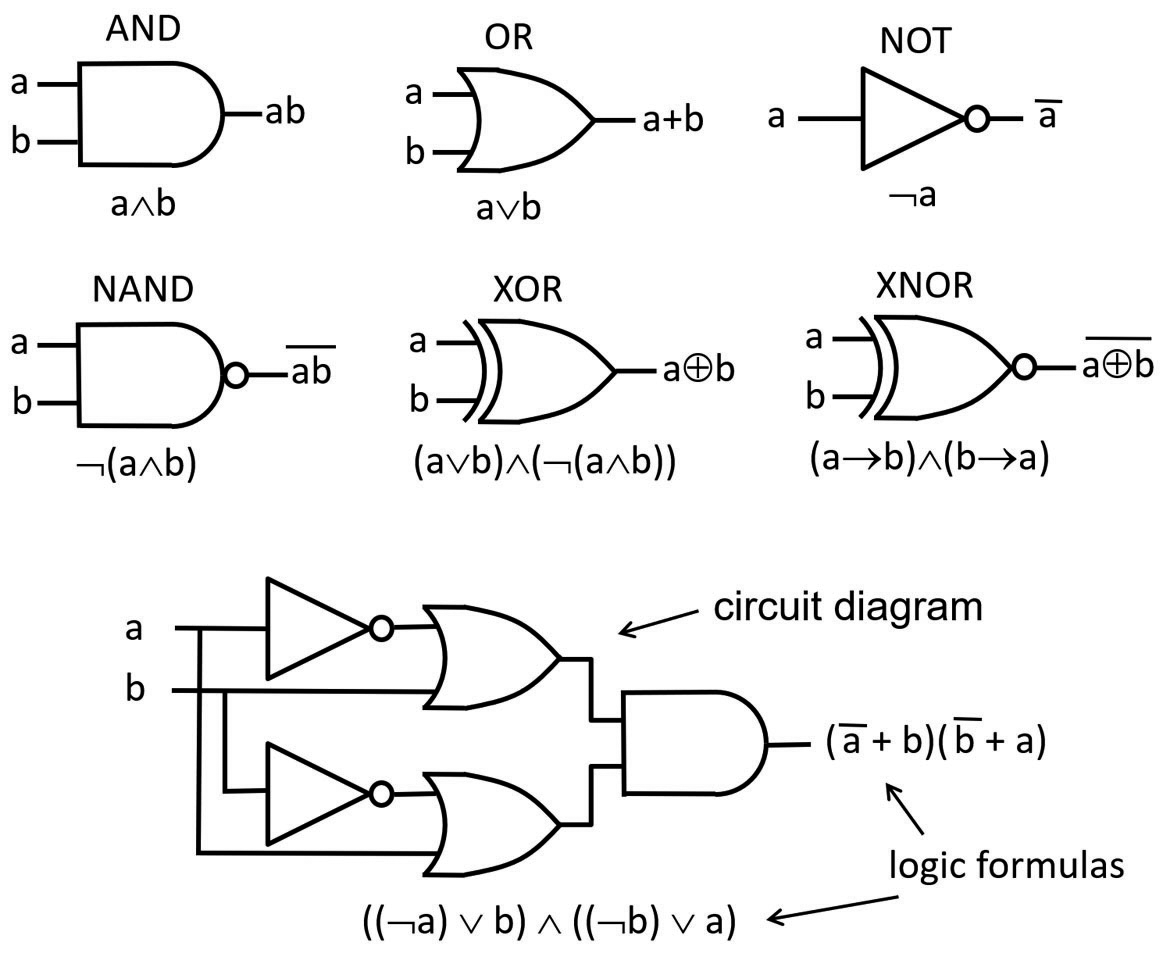
\includegraphics[scale=1]{images-cmyk/LogicGates}
%\todo{I did not have Visio with me. Improvised with PowerPoint. Figure will need to be redrawn.}
\end{center}
\index{gate!logic}\index{Boolean!gate}
\index{circuit!diagram}\index{diagram!circuit}
\index{circuit!Boolean}\index{Boolean!circuit}\index{logic!formula}\index{formula!logic}
\index{negation (not, logic gate)}\index{not (logic gate)}
\index{and (logic gate)}
\index{or (logic gate)}
\index{nand!logic gate}
\index{xor (logic gate)}
\index{xnor (logic gate)}
\index{exclusive or}\index{or, exclusive}
\index{operator, logic!nand}
\index{operator, logic!and ($\wedge$)}
\index{operator, logic!or ($\vee$)}
\index{operator, logic!nor}
\index{operator, logic!not ($\neg$)}
\index{operator, logic!exclusive or}
\index{operator, logic!exclusive nor}
\index{gate!and}
\index{gate!or}
\index{gate!not}
\index{gate!negation}
\index{inverter, gate}
\index{gate!nand}
\index{gate!nor}
\index{gate!xnor}
\index{gate!xor}
\index{gate!inverter}
\caption{Digital circuits = logic formulas.}
\label{fig-02-logic-gates}
\end{figure}

Figure~\ref{fig-02-logic-gates} (page \pageref{fig-02-logic-gates})
presents symbols used for logic gates in circuit diagrams
and annotates them with both
the algebraic notation used by circuit designers
and the logic formulas we have been using.
The important fact to remember is that all three notations
\index{circuit!diagram}\index{diagram!circuit}
represent the same concepts in logic. Circuit diagrams, logic formulas,
and the algebraic notation used by circuit designers are three
different notations for exactly the same mathematical objects.
In this sense, digital circuits, and, therefore, computers,
are materializations of logic formulas.
Computers are
\index{logic!in action}logic in action.

The logic operators that we have been using
($\wedge$, $\vee$, $\neg$, $\rightarrow$)
make it possible to write a formula
that delivers precisely the values in the truth table
for any given formula.
The \{implication\} axiom
(figure~\ref{fig-02-boolean-axioms}, page \pageref{fig-02-boolean-axioms})
expresses implication in terms of logical-or
and negation, which means we lose no expressive power by
discarding implication from the set of logic operations.

Surprisingly, the reverse is also true.
That is, for any given input/output relationship that can be expressed
in a formula using logical-and, logical-or, and negation,
there is an equivalent logic formula using implication as
the only operator. The new formula, using only the
implication operator, produces the same results
as the original formula.
The \{$\neg$ as $\rightarrow$\} equation
(figure~\ref{some-boolean-theorems}, page \pageref{some-boolean-theorems})
provides a start in this direction by showing how to express
negation in terms of the implication operator.
Furthermore, implication is not the only logic operator
that is universal in this sense.
Another one
is the negation of logical-and, which is called
\index{nand!logic gate}\index{operator, logic!nand}\emph{nand}.
When fabricated using certain widespread technologies,
nand gates can run faster and be more reliable than other gates,
so many integrated circuits make frequent use of nand gates.

It is interesting to see how to put together digital
circuits for basic operators
($\wedge$, $\vee$, and $\neg$) using only nand gates.
Consider negation, for example.
Negation has only one input signal and nand has two.
Feeding the same signal into both
inputs of a nand gate produces the behavior of
the negation operator,
as the following equation confirms:

\begin{center}
\begin{tabular}{ll}
$(\neg a) = (\neg (a \wedge a))$  & \{$\neg$ as nand\}\label{neg-as-nand}
\end{tabular}
\end{center}

In this way, a \index{gate!nand}\index{operator, logic!nand}\index{nand!logic gate}nand gate can serve in place of a
negation gate (also known as an \index{inverter, gate}\index{gate!inverter}\emph{inverter}).
There is a one-step proof of the equation,
citing the \{$\wedge$ idempotent\} theorem
(page \pageref{and-idempotent}).

A nand-only circuit for logical-and can be
\index{logic!gate}\index{gate!logic}\index{universal gate}\index{gate!universal}put
together from two nand gates in sequence.
The signal from the first nand gate is inverted
by feeding it into both inputs of a second nand gate.
Algebraically, this circuit corresponds to the following \{$\wedge$ as nand\} equation.
It takes a two-step proof to verify the equation.
The first step converts the outside nand to negation using the
\{$\neg$ as nand\} equation, and the second step cites
the \{double negation\} axiom from igure~\ref{fig-02-boolean-axioms}
(page \pageref{fig-02-boolean-axioms}).

\begin{center}
\begin{tabular}{ll}
$(a \wedge b) = (\neg ((\neg (a \wedge b)) \wedge (\neg (a \wedge b))))$ & \{$\wedge$ as nand\}\label{and-as-nand}
\end{tabular}
\end{center}

\index{negation (not, logic gate)}\index{not (logic gate)}Negation took one nand gate and
logical-and took two.
Logical-or can be implemented with three nand gates,
as shown in the following equation,
which can be verified using
the \{$\neg$ as nand\} equation, DeMorgan's laws,
and double negation:

\begin{center}
\begin{tabular}{ll}
$(a \vee b) = (\neg ((\neg(a \wedge a)) \wedge (\neg(b \wedge b))))$ & \{$\vee$ as nand\}\label{or-as-nand}
\end{tabular}
\end{center}

Figure~\ref{fig-02-nand-is-all-you-need} (page \pageref{fig-02-nand-is-all-you-need})
diagrams the digital circuits
corresponding to the formulas that express logical-and, logical-or, and negation
in terms of nand operations.

\begin{figure}
\begin{center}
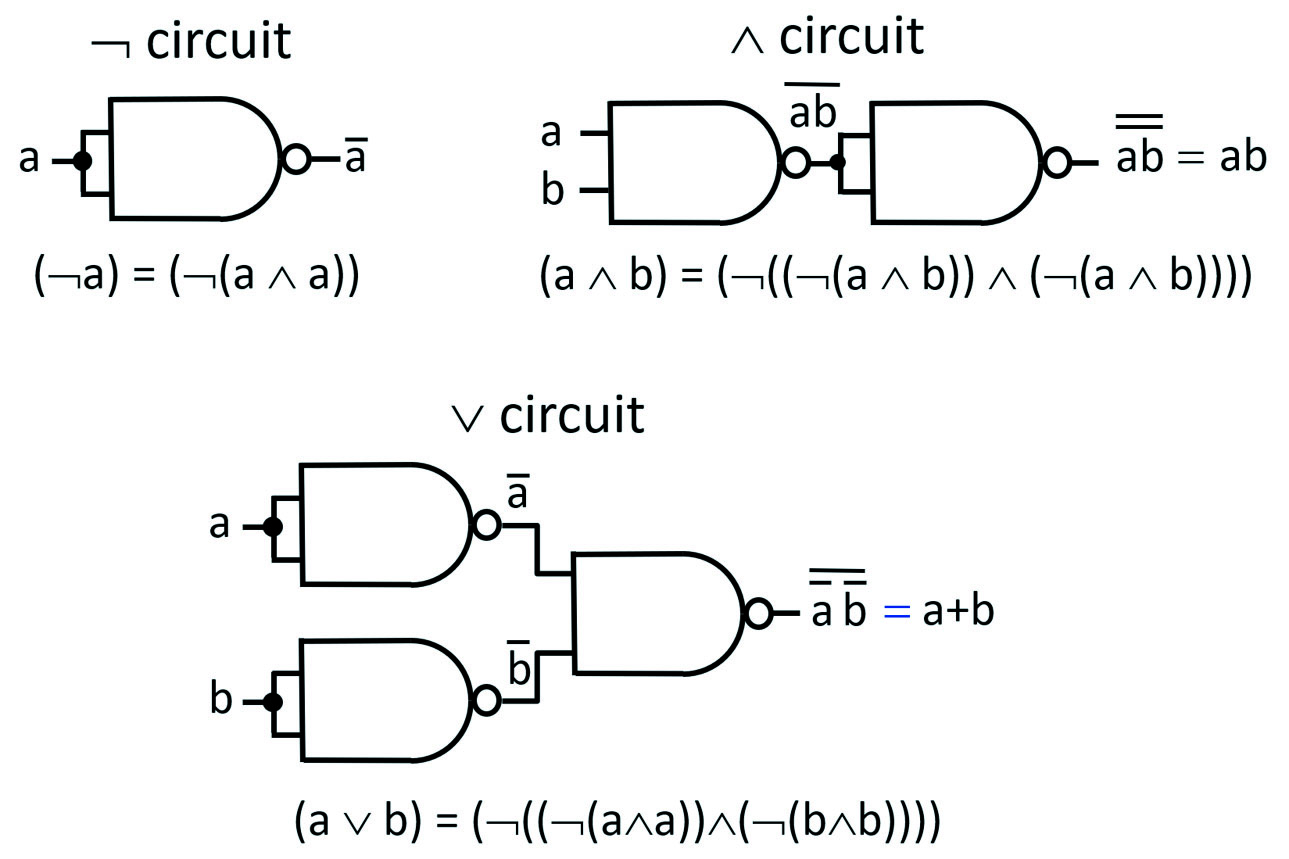
\includegraphics[scale=1]{images-cmyk/NandIsAllYouNeed}
%\todo{I did not have Visio with me. Improvised with PowerPoint. Figure will should be redrawn.}
%% redrew diagram ... still used PowerPoint, but improved the diagram a little 8Aug2017
\end{center}
\index{universal gate}
\index{gate!universal}
\index{nand!logic gate}\index{nand!is all you need}
\index{diagram!circuit}\index{circuit!diagram}
\caption{Nand is all you need.}
\label{fig-02-nand-is-all-you-need}
\end{figure}

\begin{exercises}
\exer {\label{ex:implication-gate}%
Using a negation-gate and an or-gate,
draw a circuit diagram for an ``implication circuit''
that has the same input/output behavior as the implication operator.\\
\emph{Hint}: Follow the example of the \{implication\} axiom
(figure~\ref{fig-02-boolean-axioms}, page \pageref{fig-02-boolean-axioms})).
One of the inputs will need to be a constant rather than a variable.}

\exer {For each of the following logic formulas,
draw an equivalent circuit diagram.
Since we don't have a symbol for an implication gate,
you can either make up your own symbol or
materialize logic gates where you need them
using the circuit diagram from exercise \ref{ex:implication-gate}.
\begin{center}
\begin{tabular}{l}
$((a \vee (b \wedge (\neg a))) \vee (\neg (a \vee b)))$ \\
$(((\neg a) \wedge (\neg b)) \wedge (b \wedge (\neg c)))$ \\
$(a \rightarrow (b \rightarrow c))$ \\
$((a \wedge b) \rightarrow c)$ \\
\end{tabular}
\end{center}}

\exer {Rewrite each of the formulas in the previous exercise
in the algebraic notation used by electrical engineers:
juxtaposition for $\wedge$, + for $\vee$, and $\overline{a}$ for $(\neg a)$.
Use the \{implication\} axiom to represent
implications using negation and logical-or.}

\exer {Draw circuit diagrams with behavior
of the and-gate, the or-gate, and the negation-gate
using implication operators only.}
\end{exercises}

%\todo{ do we still want to add half-adder and/or full-adder
%circuits as examples? problem: they have two outputs, so need to talk about
%tapping outputs from subformulas to show correspondence to algebraic form}

\begin{aside}{aside:struggling}{Struggling? Join the Club}
Reasoning with Boolean equations requires a lot of intellectual effort.
Almost everyone struggles when trying to master the concepts
and apply them to solve problems.
So, if you're \index{struggling?}struggling, you're normal.
If you get discouraged to the point of despair, you're normal.
It gets easier with every successful solution, but it never gets easy.
What you are doing here is real mathematics, and it places the same
kind of burden on the intellect as real \index{engineering}engineering.
Engineering is the application of principles
of math and science to the design of useful things,
so real engineering and real mathematics share a great deal of common ground.

If it does not appeal to you to struggle through many
failed attempts and beyond them to a solution, only to
go on to the next problem and start the process once again,
you are going to find engineering to be an unpleasant activity.
It's frustration, frustration, frustration
ad nauseam, then a solution, then on to the next problem.
Finding the solution through all of that fog
brings a lot of satisfaction, and for engineers and mathematicians,
that satisfaction makes it all worthwhile.

So, take heart. Keep trying.
\index{panic, don't}Hundreds of students have worked their way through the reading
and exercises of this chapter and the ones that follow,
and almost all of them have succeeded.
To do so, they invested a great deal of energy in solving problems,
reading, again and again, the examples, and applying the ideas.
Sometimes it takes many hours, just to solve one problem.
Don't give up.\index{panic, don't}\index{disheartened?}\index{frustrated?}\index{baffled?}\index{worried?}\index{scared?}\index{funk, in a?}
%\caption{Struggling? Join the Club}
%\label{aside:struggling}
\end{aside}

\section{Deduction}
\label{sec:deduction}

We have been reasoning with equations,
which means we are reasoning in two directions
at the same time. Equations go both ways.
Deductive \index{reasoning!deductive}\index{deductive reasoning}reasoning is one-directional.
It derives a conclusion from hypotheses using one-directional rules of inference.
A proof shows that the conclusion is true whenever the hypotheses are true, but it provides
no information about the conclusion when the truth of one or more of the hypotheses is
unknown.

In the following discussion of proof by \index{deduction!proof by}deduction,
theorems will be stated using a
\index{turnstile ($\vdash$)}\emph{turnstile} ($\vdash$)
to separate the \index{hypothesis!theorem}hypotheses
from the \index{conclusion!theorem}conclusions.
Hypotheses go on the left of the turnstile and the conclusion on the right.
All of the hypotheses are formulas in logic, as is the conclusion.
A turnstile asserts that there is a derivation of the conclusion
from the hypotheses using the rules of inference.
The commutativity law for logical-and, for example,
can be stated as follows:
\begin{center}
\index{theorem, by name!\{$\wedge$ commutes\}}\index{commutative}
Theorem \{$\wedge$ commutes\}: $a \wedge b \vdash b \wedge a$
\end{center}

Later, we will prove the \{$\wedge$ commutes\} theorem using a formal apparatus
for deductive reasoning known as
\index{natural deduction}\index{deduction!natural}\emph{natural deduction}.\footnote{Natural
deduction is a \index{formalism}formal system of logic pioneered in the 1930s
by the mathematician \index{Gentzen, Gerhard}Gerhard Gentzen and refined in the 1960s
by the logician \index{Prawitz, Dag}Dag Prawitz.}
\index{theorem}Theorems proved by natural deduction have zero or more
logic formulas on the left of the turnstile and exactly one formula on the right.
The formulas on the left are the \index{hypothesis}\emph{hypotheses} of the theorem and
the one on the right is the \index{conclusion}\emph{conclusion}.
A \index{proof}proof begins with the formulas on the left,
which are assumed to be true.
At each step, the proof cites either a rule of inference or a previously proven theorem
to derive a new formula. The rule or theorem ensures that when the hypotheses are true,
so is the derived formula. Derived formulas can play the role of hypotheses
in subsequent steps of the proof, and new formulas can be derived from them
in the same manner. The derived formula at the end of the proof is the conclusion.
A deductive proof of a theorem with hypothesis $h$ and conclusion $c$
verifies that the implication $(h \rightarrow c)$ is true.
\begin{center}
$h \vdash c$ ~~ensures that~~ $(h \rightarrow c) = True$
\end{center}

\begin{figure}
\begin{spacing}{0.9}
\begin{center}
\begin{tabular}{ll}
Prove $a$                                               & Prove $a \vee b$                                  \\
 - - - - - -                                            &  - - - - - - - - - -                              \\
Prove $b$                                               & Prove $a \rightarrow c$                           \\
--------------\{$\wedge$ introduction\}                 &  - - - - - - - - - -                              \\
Infer $a \wedge b$                                      & Prove $b \rightarrow c$                           \\
                                                        & -----------------\{$\vee$ elimination\}           \\
                                                        & Infer $c$                                         \\
Prove $a$                                               &                                                   \\
--------------\{$\vee$ introduction 1\}                 &                                                   \\
Infer $a \vee  b$                                       & Prove $a \wedge b$                                \\
                                                        & ----------------\{$\wedge$ elimination 1\}        \\
                                                        & Infer $a$                                         \\
Prove $b$                                               &                                                   \\
--------------\{$\vee$ introduction 2\}                 &                                                   \\
Infer $a \vee  b$                                       & Prove $a \wedge b$                                \\
                                                        & ----------------\{$\wedge$ elimination 2\}        \\
                                                        & Infer $b$                                         \\
Prove $a \rightarrow False$                             &                                                   \\
-----------------------\{$\neg$ introduction\}          &                                                   \\
Infer $\neg a$                                          & Prove $\neg a$                                    \\
                                                        & ---------------------\{$\neg$ elimination\}       \\
                                                        & Infer $a \rightarrow False$                       \\
Prove $a$                                               &                                                   \\
----------\{identity\}                                  &                                                   \\
Infer $a$                                               & Prove \emph{False}                                \\
                                                        & ---------------\{contradiction\}                  \\
                                                        & Infer $a$                                         \\
Prove $a$                                               &                                                   \\
 - - - - - - - - - -                                    &                                                   \\
Prove $a \rightarrow b$                                 & Prove $(\neg a) \rightarrow$ \emph{False}         \\
-----------------\{modus ponens\}                       & --------------------------\{reductio ad absurdum\}\\
Infer $b$                                               & Infer $a$                                         \\
                                                        &                                                   \\
\end{tabular}
\end{center}
\begin{center}
\begin{tabular}{ll}
Assume $a$                                      & \emph{assumption required to cite} \{$\rightarrow$ introduction\}     \\
--------------\{\emph{r}\}                      & \emph{r is an inference rule or proven theorem}                       \\
Prove $b$                                       & $b$ \emph{has now been derived from assumption} $a$                   \\
-----------------\{$\rightarrow$ introduction\} & \emph{proof above line begins with} ``Assume \emph{left operand''}    \\
Infer $a \rightarrow b$                         & ~~~~\emph{and concludes with right operand, proving} $a \rightarrow b$\\
Discharge $a$                                   & \emph{excludes formula} ``$a$'' \emph{from hypotheses of theorem}     \\
\end{tabular}
\end{center}
\end{spacing}
\index{hypothesis!Assume (natural deduction)}
\index{Assume (natural deduction)}\index{proof!Assume (natural deduction)}
\index{inference rule, by name!\{$\wedge$ introduction\}}
\index{inference rule, by name!\{$\vee$ introduction 1\}}
\index{inference rule, by name!\{$\vee$ introduction 2\}}
\index{inference rule, by name!\{$\vee$ elimination\}}
\index{inference rule, by name!\{$\neg$ introduction\}}
\index{inference rule, by name!\{identity\}}
\index{inference rule, by name!\{modus ponens\}}
\index{inference rule, by name!\{$\wedge$ elimination 1\}}
\index{inference rule, by name!\{$\wedge$ elimination 2\}}
\index{inference rule, by name!\{$\neg$ elimination\}}
\index{inference rule, by name!\{contradiction\}}
\index{inference rule, by name!\{reductio ad absurdum\}}
\index{inference rule, by name!\{$\rightarrow$ introduction\}}
\index{inference rule!table of}
\index{modus ponens}
\index{contradiction!inference rule}
\seeonlyindex{elimination rule}{inference rule}
\seeonlyindex{introduction rule}{inference rule}
\index{identity}
\index{reductio ad absurdum}
\index{deductive proof}
\index{natural deduction}
\index{deduction!natural}
\index{discharge assumption}\index{Assume (natural deduction)!discharge}\index{hypothesis!discharge}
\index{inference rule!discharge assumption}
\index{proof!deductive}
\caption{Rules of inference for natural deduction.}
\label{fig-02-deduction-rules}
\end{figure}

Of course, the truth of an implication formula doesn't
say anything about the value of the
left-hand operand of the implication operator.
That value could be either $True$ or $False$.
The implication formula just says that
the only combination of values that can make
$(h \rightarrow c)$ have the value $False$
(namely, $h = True$, $c = False$, as verified in
theorem \{$\rightarrow$ truth table\},
page \pageref{implication-truth-table}) cannot occur.
In the same way, a deductive proof of a theorem
does not provide any information about the hypotheses.
It only says that the conclusion will be true
whenever all of the hypotheses are true.

\begin{figure}
%\begin{quote}
Theorem \{Socrates was mortal\}: $man$, $man \rightarrow mortal$ $\vdash$ $mortal$ \\
\emph{proof}
%\end{quote}
\begin{center}
\begin{spacing}{0.9}
\begin{tabular}{l}
Assume $man$                    \\
 - - - - - - - - - - - - - - - - - -\\
Assume $man \rightarrow mortal$ \\
--------------------------------\{modus ponens\} \\
~~~~~~ $mortal$                 \\
\end{tabular}
\end{spacing}
\end{center}\index{inference rule, by name!\{modus ponens\}}\index{modus ponens}\index{Socrates syllogism}\index{syllogism!Socrates}\index{theorem!Socrates}\index{Assume (natural deduction)}
\caption{Theorem \{Socrates was mortal\}: citing modus ponens.}
\label{fig:socrates-proof}
\end{figure}

Sometimes a theorem has several hypotheses.
A proof by deductive reasoning of the theorem
$h_1$, $h_2$ $\vdash$ $c$,
which has two hypotheses,
ensures that
$((h_1 \wedge h_2) \rightarrow c) = True$.
A theorem with no hypotheses at all
would have no formulas on the left-hand side of the turnstile:
$\vdash c$.
A proof of such a theorem would
verify the equation $c = True$.

All of the axioms of Boolean algebra
(figure~\ref{fig-02-boolean-axioms}, page \pageref{fig-02-boolean-axioms})
can be derived through deductive reasoning.
Many presentations of classical logic begin with
\index{deductive reasoning}deductive \index{reasoning!deductive}reasoning,
but we started with Boolean algebra
because we will be using logic to reason about
digital circuits and software specified in the form of equations.
So, equations play a central role throughout the
discussion.\footnote{An accessible,
more extensive discussion of natural deduction can be found
in O'Donnell, Hall, and Page,
\emph{Discrete Mathematics Using a Computer}
(2\textsuperscript{nd} ed.), Springer, 2006.}

Figure~\ref{fig-02-deduction-rules} (page \pageref{fig-02-deduction-rules})
provides schematics of the rules of inference of \emph{natural deduction}.
A citation of an inference rule derives a \index{conclusion}new formula
from hypotheses (assumed true) or from formulas derived through prior reasoning in the proof.
Each \index{citation!inference rule}\index{inference rule!citation}rule citation
has three parts:
%\begin{quote}
\begin{enumerate}
\item A proof above the line (or multiple proofs, depending on the rule),
\item a line annotated with the name of the cited inference rule, and
\item exactly one logic formula below the line.
\end{enumerate}
%\end{quote}

\label{def-deductive-proof}
A \emph{deductive proof} is a sequence of citations of inference rules
in which the final citation has, below the line,
the formula that is the conclusion of the theorem that the proof verifies.
An inference rule can place specific constraints on the formula
that is its conclusion and/or on the formulas that are the
conclusions of the proofs that the rule requires above the line.
For example, the \{$\wedge$ elimination 1\} inference rule
(figure~\ref{fig-02-deduction-rules}, page \pageref{fig-02-deduction-rules})
requires one \index{proof!deductive}proof
\index{proof!above/below the line}above the line
and constrains the conclusion of that proof
to be a logical-and formula $(a \wedge b)$.
The \{$\wedge$ introduction\} rule, on the other hand,
requires two proofs above the line and
constrains its conclusion (below the line)
to be a logical-and formula $(a \wedge b)$.
Some rules place constraints both on the formulas
above the line (which have been derived earlier in the proof)
and on the formula
\seeonlyindex{above the line}{proof}\seeonlyindex{below the line}{proof}\index{line (natural deduction)!above/below}below the line.
For example, the \{$\neg$ introduction\} rule requires
the formula above the line to be an implication
whose conclusion is the logical constant \emph{False}
($a \rightarrow False$)
and constrains the formula below the line to be
a negation formula ($\neg a$).
Furthermore, the hypothesis of the implication above the line must be the same
formula that is negated below the line.

When a rule is
\index{citation!inference rule}\index{inference rule!citation}\seeonlyindex{rule of inference}{inference rule}cited
in a deductive proof,
the name of the rule is written just to the right of
the line that separates the proofs that the rule requires above the line
from the conclusion that the citation derives,
which is the formula written below the line.
When an inference rule requires multiple proofs above the line,
dashed lines separate those proofs.
Each of the proofs that the rule requires above the line
is itself a proof.
That is, it is also a sequence of citations ending in a conclusion formula.

The \index{scope!inference rule citation}\index{inference rule!scope of citation}\emph{scope} of a
\index{citation!inference rule}\index{inference rule!citation}citation
of an inference rule
extends upward to the beginning of the first of the proofs
above the line that the rule requires.
The scopes of citations in a proof can overlap,
and when they do, some proofs are nested inside others.
In fact, the scope of the last citation of a rule in a proof
always extends upward to the beginning of the proof,
so the scopes of all of the other citations are nested
within the scope of the last citation.\footnote{Because
of nested scopes,
proofs by natural deduction
are sometimes written with parentheses,
like algebraic formulas,
or displayed as ``tree diagrams,''
with the conclusion of the theorem at the bottom and
the citations spread out upwards
in a branching structure
that makes the overlapping (and nonoverlapping)
of scopes easy to see.
We have chosen a vertical format with implicit
overlapping because this notation is more compact than a
\index{natural deduction!tree diagram}\index{proof!tree diagram}tree
diagram and, in our judgment,
more readable than a parenthesized proof formula.}

Wherever an inference rule requires a proof above the line,
an assumption can take the place of that proof.
That is,
an assumption can always stand in lieu of a proof.
A logic formula that is marked as an assumption
is a hypothesis of the theorem verified by the proof
(unless that assumption is subsequently \emph{discharged},
a special dispensation
that will be discussed later).
So, any proof may begin with a formula
that is marked as an assumption.
However, no proof can have
a formula marked as an assumption after
the first citation of a rule in the proof.
\index{proof!assumption}Assumptions
can appear only above the line
of the first citation in the sequence of citations
comprising the proof, but since citations
(and therefore proofs) can be nested,
an assumption need not be the first line in
the entire proof.
It may, instead, be the first line
in a proof that is nested inside another proof.

The \index{modus ponens}\{modus ponens\} rule
(figure \ref{fig-02-deduction-rules}, page \pageref{fig-02-deduction-rules})
is probably the most widely recognized rule of inference because
of the well-known ``Socrates was mortal'' syllogism
(figure \ref{fig:socrates-proof}, page \pageref{fig:socrates-proof}).
The rule says that if there is a proof concluding in
the formula $a$ and a proof concluding in the formula ($a \rightarrow b$),
those proofs, together with a citation of modus ponens,
derive the conclusion $b$.\footnote{Deductive
proofs are one-directional,
and so is the theorem about Socrates.
One can conclude mortality from two hypotheses about circumstances of life,
but one cannot derive those circumstances from the mortality of Socrates.
Rabbits, for example, are mortal, but they are not men.}

Proofs by natural deduction follow a strictly prescribed format,
and it is worth going over that format again in slightly different terms.
The proof of a theorem that has
$n$ hypotheses will have $n$ different
formulas representing those hypotheses
marked as assumptions
at the beginning of one or more of the proofs
required by the inference rules that the proof cites.
That is, each hypothesis, at the point where it is introduced
into the proof, is marked as an assumption.
An assumption so marked stands in lieu of the proof
required at that point by whatever inference rule is being cited.
A particular formula in a proof may be marked as an assumption
at more than one point in a proof, but no matter how many places
it appears as an assumption, it is still just
one hypothesis of the theorem being proved.
A proof of a theorem with $n$ hypotheses will have at least $n$
formulas marked as assumptions.
It will have more than $n$ formulas marked as assumptions
if two or more of the assumptions specify the same formula
(or if a formula is discharged).

Assumptions must appear at the beginning of
a proof, before the citation of any
inference rule in the proof.
Assumptions cannot pop up after the citation
of an inference rule in a proof.
Of course, since \index{proof!dashed line}\index{line (natural deduction)!dashed}dashed
lines indicate separate proofs,
the \index{Assume (natural deduction)}assumption need not be at the beginning of the entire
proof, but it could, instead, be at the beginning of
a proof separated from another proof by a dashed line.
The \{Socrates was mortal\} theorem
(figure \ref{fig:socrates-proof})
has two hypotheses.
One is marked as an assumption standing in lieu of the first proof
required by a citation of \{modus ponens\}
and the other is marked as an assumption
standing in lieu of the second proof
required by \{modus ponens\}.

Three of the inference rules of natural deduction
(figure \ref{fig-02-deduction-rules})
involve the $\wedge$ operator:
\{$\wedge$ introduction\},
\{$\wedge$ elimination 1\}, and
\{$\wedge$ elimination 2\}.
Using these rules, we can construct a deductive proof
of the commutativity law for $\wedge$,
and the proof will serve as a reasonably straightforward
example to get started with natural deduction.

\begin{figure}
Theorem \{$\wedge$ commutes\}: $a \wedge b$ $\vdash$ $b \wedge a$ \\
\emph{proof}
\begin{center}
\begin{spacing}{0.9}
\begin{tabular}{ll}
Assume $a \wedge b$                             &\emph{hypothesis of theorem}\\
-------------------\{$\wedge$ elimination 2\}   &\\
~~~~~~~~~~$b$                                   &\emph{concludes 1$^{\text{st}}$ proof for} \{$\wedge$ introduction\}\\
 - - - - - - - - - - - - - - - - - - - - - - - -&\emph{separates proofs for} \{$\wedge$ introduction\}\\
Assume $a \wedge b$                             &\emph{hypothesis of theorem (reused)}\\
-------------------\{$\wedge$ elimination 1\}   &\\
~~~~~~~~~~$a$                                   &\emph{concludes 2$^{\text{nd}}$ proof for} \{$\wedge$ introduction\}\\
-------------------\{$\wedge$ introduction\}    &\emph{scope extends to top}\\
~~~~~~~~$b \wedge a$                            &\emph{proved} $b$, \emph{proved} $a$, \emph{conclude} $(b \wedge a)$\\
\end{tabular}
\end{spacing}
\end{center}\index{hypothesis!Assume (natural deduction)}\index{Assume (natural deduction)}\index{proof!Assume (natural deduction)}\index{inference rule, by name!\{$\wedge$ elimination 2\}}\index{inference rule, by name!\{$\wedge$ elimination 1\}}\index{inference rule, by name!\{$\wedge$ introduction\}}\index{proof!deductive}\index{theorem, by name!\{$\wedge$ commutes\}}\index{commutative}
\caption{\{$\wedge$ commutes\}: citing three inference rules involving $\wedge$.}
\label{fig:and-commutes-proof}
\end{figure}

The proof in
Figure \ref{fig:and-commutes-proof} (page \pageref{fig:and-commutes-proof})
cites the \{$\wedge$ introduction\} inference rule,
a rule that requires two proofs above the line.
The first of those proofs, in this example, has the hypothesis
of the theorem above the line, marked as an assumption.
It then cites the \{$\wedge$ elimination 2\} rule,
which requires the right-hand operand ($b$) of the $\wedge$
above the line to go under the line as the conclusion.
Then comes the dashed line separating
the two proofs required by \{$\wedge$ introduction\}.
The second of the proofs comes next.
It has the same form as the first proof
except that it cites \{$\wedge$ elimination 1\} instead of \{$\wedge$ elimination 2\}.
The \{$\wedge$ elimination 1\} rule brings the left-hand operand ($a$) of the $\wedge$
down below the line.
The \{$\wedge$ introduction\} rule requires the
conclusion of the first proof above line to
become the left-hand operand of the $\wedge$
operation that the rule introduces,
and it requires the conclusion of the second
proof to be the right-hand operand.
The $\wedge$ formula with those two operands
is the conclusion below the line citing the \{$\wedge$ introduction\} inference rule.
That final citation completes the proof of the \{$\wedge$ commutes\} theorem.

To recap, the proof of the {\{$\wedge$ commutes\} theorem
consisted of three proofs, in a sense,
one being the whole proof, ending in the citation of
the \{$\wedge$ introduction\} rule,
and the other two being the proofs required by the citation of \{$\wedge$ introduction\}.
Each of the three proofs in this example consisted of exactly one rule citation.
Sometimes there are several rule citations in a proof, sometimes only one,
and sometimes, when the proof is an assumption, none.

\begin{aside}{variable-stand-for-formulas}{Variables Stand for Formulas}
As in Boolean algebra, variables in deductive reasoning
stand for arbitrary formulas.
Any grammatically correct formula
can be plugged in for a variable in a theorem,
as long as all of the instances of that variable are
replaced by that same formula.
For example,
theorem \{$\wedge$ commutes\} ($a \wedge b$ $\vdash$ $b \wedge a$)
has two variables, $a$ and $b$.
Since ($x \vee y$) and ($y \rightarrow z$) are formulas,
the theorem justifies the following more specialized
version:
\begin{center}
$(x \vee y) \wedge (y \rightarrow z)$ $\vdash$ $(y \rightarrow z) \wedge (x \vee y)$
\end{center}
The theorem also justifies the following restatement of the
theorem that uses the formula $b$ in place of $a$ and the formula $a$ in place of $b$.
\begin{center}
$b \wedge a$ $\vdash$ $a \wedge b$
\end{center}
Variables are used in this manner throughout the book. Nothing new here.
We bring it up again because it is important
to keep in mind when citing inference rules
or theorems.\index{variable}\index{formula!variables}
%\caption{Variables Stand for Formulas}
%\label{variable-stand-for-formulas}
\end{aside}

Two formulas are annotated as assumptions in the
proof of the \{$\wedge$ commutes\} theorem.
This suggests that the theorem has
two hypotheses,
but in this case, both assumptions are the same formula.
A particular formula can be used as many times as necessary as
an assumption in a proof, but it only counts as one hypothesis
in the theorem.
The number of hypotheses
of the theorem is the number of distinct
formulas annotated as assumptions in the proof
minus the number of those assumptions that are discharged
by citations of the \{$\rightarrow$ introduction\} inference rule,
which we will discuss shortly.

\begin{figure}
Theorem \{self-implication\}: $\vdash$ $a \rightarrow a$ ~~~~\emph{Note: This theorem has no hypotheses.}\\
proof
\begin{center}
\begin{spacing}{0.9}
\begin{tabular}{ll}
Assume $a$                  &\emph{assumption discharged later}\\
---------------\{identity\} &\\
~~~~~$a$                    &\\
---------------\{$\rightarrow$ introduction\} &\\
~~$a \rightarrow a$         &\emph{assumed} $a$\emph{, proved} $a$\emph{, conclude} $a \rightarrow a$\\
~~Discharge $a$             &\emph{discharged by} \{$\rightarrow$ introduction\} \emph{citation}, \emph{as promised}\\
\end{tabular}
\end{spacing}
\end{center}\index{hypothesis!Assume (natural deduction)}\index{Assume (natural deduction)}\index{proof!Assume (natural deduction)}\index{inference rule, by name!\{identity\}}\index{inference rule, by name!\{$\rightarrow$ introduction\}}\index{hypothesis!discharge}\index{discharge assumption}\index{Assume (natural deduction)!discharge}\index{inference rule!discharge assumption}\index{theorem, by name!\{self-implication\}}
\caption{\{self-implication\}: citing  \{identity\} and \{$\rightarrow$\ introduction\} inference rules.}
\label{fig:or-self-imp-proof}
\end{figure}

Given a proof, it is straightforward to extract
the theorem it proves.
On the left of the turnstile ($\vdash$), put all of the different
formulas annotated as assumptions in the proof
except those that are discharged.
After the turnstile, write the formula in the
conclusion at the end of the proof.

Now we come to the issue of
\index{hypothesis!discharge}\index{discharge assumption}\index{Assume (natural deduction)!discharge}\index{inference rule!discharge assumption}\index{proof!discharge assumption}\index{Assume (natural deduction)!discharge}discharging
formulas assumed in proofs.
The inference rule \{$\rightarrow$ introduction\}
has some unique characteristics.
It requires only one proof above the line,
but that proof must begin with a formula
(let's call it $a$)
marked as an assumption.
To repeat, the proof above the line in a citation of
\{$\rightarrow$ introduction\} that
concludes with the formula $(a \rightarrow b)$
below the line
must begin with ``Assume $a$'' and
then continue from there to derive the formula $b$, just above the line.
The scope of the \{$\rightarrow$ introduction\} citation
extends upward to the required assumption.

Normally, any formula assumed at the beginning of a proof
becomes a \index{hypothesis}hypothesis of the theorem that was proved.
However, a
\index{hypothesis!discharge}\index{discharge assumption}\index{Assume (natural deduction)!discharge}\index{inference rule!discharge assumption}\index{proof!discharge assumption}discharged
assumption
is not added to the hypotheses of the theorem.
A citation of the
\index{inference rule, by name!\{$\rightarrow$ introduction\}}\{$\rightarrow$ introduction\} rule
triggers a discharge of the assumed formula that the
rule requires at the beginning of the proof above the line.
(Without that assumption, the citation,
and therefore the proof, is not valid.)
The reason for the discharge is that the truth of an implication
formula doesn't place any constraints on the value of its
left-hand operand.
The implication says that if the left-hand operand
has the value \emph{True}, then so does the right-hand operand,
and the proof confirms that relationship.
Since the citation of the
\{$\rightarrow$ introduction\} rule
simply confirms that the implication formula below the line
is true, the citation places no constraints on the value
of the left-hand operand.
The assumption only applies within the scope
of the citation of the \{$\rightarrow$ introduction\} inference rule
and therefore does not become a hypothesis of the theorem being proved
(unless it is assumed elsewhere in the proof and not discharged).

Figure \ref{fig:or-self-imp-proof} (page \pageref{fig:or-self-imp-proof})
displays a proof of the \{self-implication\} theorem,
which says that formulas of the form ($a \rightarrow a$) always have the value \emph{True}.
The proof cites the \{identity\} rule,
which is included among the inference rules to make it
possible for proofs by natural deduction to stay strictly
within the formalism required by the system.
The \{identity\} rule says that a proof of formula $a$
can be followed by a citation of the \{identity\} rule
with that same formula, $a$, as its conclusion below the line.

The application of any rule must \index{matching!inference rule}\index{inference rule!matching}match
the template in the specification of the rule,
and the \{identity\} rule is sometimes needed to make it possible to match a template.
That is what happens in the proof of self-implication (figure \ref{fig:or-self-imp-proof}).
The proof cites the \{$\rightarrow$ introduction\} rule
to derive the formula $(a \rightarrow a)$,
and that citation requires
a proof above the line that begins with the assumption of $a$
and concludes with the formula $a$ just above the line.
The \{identity\} rule makes it possible to satisfy this requirement.
In the proof of self-implication,
the citation of the
\index{implication ($\rightarrow$)!introduction}\{$\rightarrow$ introduction\} rule
follows the derivation of $a$ from $a$ and triggers a
\index{discharge assumption}discharge
of the assumption of $a$ at the beginning of the proof.
There are no other \index{Assume (natural deduction)}assumed formulas in the proof,
so the theorem proved has no hypotheses.
That is, the \index{proof}proof confirms that the
\index{conclusion}conclusion formula
$(a \rightarrow a)$ has the value $True$, regardless of
what formula $a$ stands for.

\begin{figure}
Theorem \{$\vee$ commutes\}: $a \vee b$ $\vdash$ $b \vee a$ \\
\emph{proof}
\begin{center}
\begin{spacing}{0.9}
\begin{tabular}{ll}
Assume ($a \vee b$)          &\emph{hypothesis of theorem}\\
 - - - - - - - - - - - - - - - - - - - - - -&\emph{separates 1\textsuperscript{st} and 2\textsuperscript{nd} proofs for} \{$\vee$ elimination\} \\
Assume $a$          &\emph{this assumption will be discharged}\\
--------------\{$\vee$ introduction 2\} &\emph{allows arbitrary left-hand operand in conclusion}\\
~~$(b \vee a)$        &\\
-----------------\{$\rightarrow$ introduction\} &\emph{assumed} $a$\emph{, proved} $(b \vee a)$\emph{, conclude} $a \rightarrow (b \vee a)$ \\
~$a \rightarrow (b \vee a)$ &\{$\vee$ elimination\} \emph{requires this conclusion here}\\
Discharge $a$              &\emph{discharged by} \{$\rightarrow$ introduction\} \emph{citation, as promised}\\
 - - - - - - - - - - - - - - - - - - - - - -&\emph{separates 2\textsuperscript{nd} and 3\textsuperscript{rd} proofs for} \{$\vee$ elimination\}\\
Assume $b$          &\emph{this assumption will be discharged}\\
--------------\{$\vee$ introduction 1\} &\emph{allows arbitrary right-hand operand in conclusion}\\
~~$(b \vee a)$        &\\
-----------------\{$\rightarrow$ introduction\} &\emph{assumed} $b$\emph{, proved} $(b \vee a)$\emph{, conclude} $b \rightarrow (b \vee a)$\\
~$b \rightarrow (b \vee a)$ &\{$\vee$ elimination\} \emph{requires this conclusion here}\\
Discharge $b$               &\emph{discharged by} \{$\rightarrow$ introduction\} \emph{citation, as promised}\\
---------------\{$\vee$ elimination\}       &\emph{scope extends up to} Assume $(a \vee b)$\\
~~~~$(b \vee a)$        &\emph{3 req'd proofs above, conclude} $(b \vee a)$\\
\end{tabular}
\end{spacing}
\end{center}
\index{hypothesis!Assume (natural deduction)}\index{Assume (natural deduction)}\index{proof!Assume (natural deduction)}\index{inference rule, by name!\{$\vee$ elimination\}}\index{inference rule, by name!\{$\vee$ introduction 2\}}\index{inference rule, by name!\{$\rightarrow$ introduction\}}\index{inference rule, by name!\{$\vee$ introduction 1\}}\index{inference rule!discharge assumption}\index{discharge assumption}\index{Assume (natural deduction)!discharge}\index{hypothesis!discharge}\index{theorem, by name!\{$\vee$ commutes\}}\index{commutative}
\caption{\{$\vee$ commutes\}: citing \{$\vee$ elimination\}.}
\label{fig:or-commutes-proof}
\end{figure}

We now take on a theorem whose proof is more complex
than those we have studied so far.
The \{$\wedge$ commutes\} theorem proved earlier
is similar to the \{$\vee$ commutes\} theorem
that we will discuss now, but the proofs are very different.
Figure \ref{fig:or-commutes-proof} (page \pageref{fig:or-commutes-proof}),
which displays the proof of the \{$\vee$ commutes\} theorem,
cites all three of the inference rules involving the $\vee$ operator
and affords an example of how the \{$\vee$ elimination\} rule works.

The \{$\vee$ elimination\} rule calls for three proofs above the line.
\index{inference rule, by name!\{$\vee$ elimination\}}The
first of the three proofs must conclude in a formula
that is a logical-or, $(a \vee b)$, where, of course,
$a$ and $b$ can be any grammatically correct logic formulas.
The second proof must conclude in an implication, $a \rightarrow c$.
In this implication, $a$ is the left-hand operand of the $\vee$ formula
that concluded the first proof above the line,
and $c$ (which of course can be a formula rather than just a variable)
is the conclusion under the line citing the \{$\vee$ elimination\} rule.
The third proof must conclude in an implication, $b \rightarrow c$,
with the same right-hand operand as the implication that concludes
the second proof but with a left-hand operand that is the same
as the right-hand operand of the logical-or that concludes the
first proof above the line.
The \{$\vee$ elimination\} rule is complicated
but surprisingly easy to cite
because the rule places so many constraints on its various parts.

The proof in figure~\ref{fig:or-commutes-proof} cites both of the
``or introduction'' rules:
\{$\vee$ introduction 1\} and \{$\vee$ introduction 2\}.
These rules allow the introduction of an arbitrary formula
into the proof.
That is, when you cite the rule, you can make up one of the
formulas in the conclusion (namely, the right-hand operand of
the logical-or in the case of \{$\vee$ introduction 1\}
and the left-hand operand in the case of \{$\vee$ introduction 2\}).
The formula you choose can be as complicated or as simple as you like,
whatever is needed to make the proof work.
In the proof at hand,
the made-up formulas are simple ($b$ in one case and $a$ in the other case),
but they are exactly what the proof needs.

In addition to citing all three inference rules involving the $\vee$ operator,
the proof cites the \{$\rightarrow$ introduction\} rule twice.
Both of those citations require discharges,
so there's lot of action in the proof.
Figure~\ref{fig:or-commutes-proof}
elucidates the details with commentary
intended to help you work through the proof
to understand how the citations fit together and
comprise a proof of the \{$\vee$ commutes\} theorem.

Deductive proofs are one-directional,
so it's a little ironic that most
of the theorems we've prove so far using natural deduction
turn out to be bidirectional.
The proofs went in only one direction,
but the theorems were provable in the other direction, too.

The theorem that we turn to now, the implication chain rule
(figure \ref{fig:impchain-proof}, page \pageref{fig:impchain-proof}),
only goes in one direction.
It derives a conclusion from two hypotheses,
but the two hypotheses cannot be derived from the conclusion.
Again, commentary with the proof is intended
to help you work your way through it.
Pay particular attention to the discharge of the
assumption that is introduced at the top of the proof.

\begin{figure}
Theorem \{$\rightarrow$ chain\}
$(a \rightarrow b)$, $(b \rightarrow c)$ $\vdash$ $a \rightarrow c$ \\
\emph{proof}
\begin{center}
\begin{spacing}{0.9}
\begin{tabular}{ll}
Assume $a$                                             &\emph{assumption discharged later}\\
 - - - - - - - - - - - - - - - - - - - - - - - -       &\emph{separates proofs required by} \{modus ponens\}\\
Assume $a \rightarrow b$                               &\emph{hypothesis of theorem}\\
-----------------------\{modus ponens\}                &\{modus ponens\} \emph{citation} $\dots$\\
~~~~~~~~~~~~$b$                                        &~~~~~\emph{scope of citation extends up to} Assume $a$\\
 - - - - - - - - - - - - - - - - - - - - - - - -       &\emph{separates proofs for second} \{modus ponens\} \\
Assume $b \rightarrow c$                               &\emph{hypothesis of theorem}\\
------------------------\{modus ponens\}               &\emph{second citation of} \{modus ponens\} $\dots$\\
~~~~~~~~~~~~$c$                                        &~~~~~\emph{scope overlaps first citation} \\
------------------------\{$\rightarrow$ introduction\} &\\
~~~~~($a \rightarrow c$)                               &\emph{assumed} $a$\emph{, proved} $c$\emph{, conclude} $(a \rightarrow c)$ \\
~~~~~Discharge $a$                                     &\emph{discharged by citation of} \{$\rightarrow$ introduction\}\\
\end{tabular}
\end{spacing}
\end{center}
\index{hypothesis!Assume (natural deduction)}
\index{Assume (natural deduction)}\index{proof!Assume (natural deduction)}
\index{inference rule, by name!\{modus ponens\}}
\index{inference rule, by name!\{$\rightarrow$ introduction\}}
\index{modus ponens}
\index{theorem, by name!\{$\rightarrow$ chain\}}
\index{inference rule!discharge assumption}
\index{discharge assumption}\index{Assume (natural deduction)!discharge}
\index{hypothesis!discharge}
\caption{Proving the implication chain rule.}
\label{fig:impchain-proof}
\end{figure}

In \index{proof!deductive}deductive proofs, previously proven theorems
can be cited as if they were
\index{inference rule!theorem as}\index{theorem!as inference rule}inference rules.
Of course, the proof could always be carried out using inference rules alone
by copying the proof of the cited theorem in place of its citation,
but that leads to very long proofs, just as writing a computer program
without defining and invoking procedures encapsulating common operations
leads to very long programs. Long proofs, like long programs, tend
to be unreliable, maybe because it's so difficult
to analyze such a large mass of
detail without getting confused.
But even if they weren't unreliable, they would be an eyesore,
not to mention difficult to fix if there were an error.
That's why the ability to cite proven theorems in
deductive proofs is important. It makes them shorter
and easier to comprehend incrementally, one short proof at a time.

\begin{figure}
Theorem \{modus tollens\}: $a \rightarrow b$, $\neg b$ $\vdash$ $\neg a$\\
\emph{proof}
\begin{center}
\begin{spacing}{0.9}
\begin{tabular}{ll}
Assume $a \rightarrow b$                      &\emph{hypothesis of theorem}\\
 - - - - - - - - - - - - - - - - - - - -      &\emph{separates proofs of hypotheses of} \{$\rightarrow$ chain\} \emph{theorem}\\
Assume $\neg b$                               &\emph{hypothesis of theorem}\\
---------------\{$\neg$ elimination\}         &\\
$b \rightarrow False$                         &\\
---------------\{$\rightarrow$ chain\}        & \emph{citing theorem with 2 hypotheses} $\dots$\\
$a \rightarrow False$                         &~~~~~~~~\emph{scope extends to top of proof}\\
---------------\{$\neg$ introduction\}        &\\
~~~~$\neg a$                                  &\\
\end{tabular}
\end{spacing}
\end{center}
\index{hypothesis!Assume (natural deduction)}
\index{Assume (natural deduction)}\index{proof!Assume (natural deduction)}
\index{inference rule, by name!\{$\neg$ elimination\}}
\index{inference rule, by name!\{$\neg$ introduction\}}
\index{modus tollens}
\index{theorem, by name!\{modus tollens\}}
\caption{\{modus tollens\}: citing a theorem to justify an inference.}
\label{fig:modtol-proof}
\end{figure}

The citation of a theorem in a proof must be preceded by proofs of
each of its hypotheses above the line, just as
each inference rule citation must be preceded by a certain number of proofs above the line.
As with inference rules that require multiple proofs above the line,
we use a dashed line to separate the required proofs
when citing a theorem that has more than one hypothesis and therefore
requires more than one proof above the line.
Figure \ref{fig:modtol-proof} (page \pageref{fig:modtol-proof})
displays a proof of the modus tollens theorem.\footnote{The
inference rule \{modus ponens\} says that the conclusion of an implication
can be derived from a proof of its hypothesis.
The modus tollens theorem says that the hypothesis
of an implication can be derived from
a proof of the negation of its conclusion.}
The proof cites the implication chain rule theorem.
Since that theorem has two hypotheses, there are two proofs above
the line where the theorem is cited. Those proofs conclude in
the implication formulas that are the hypotheses of the implication chain rule.
Finally, the a citation of the \{$\neg$ introduction\} rule completes the proof.

The \{reductio ad absurdum\} rule supports
``proof by contradiction.''
It says that if you can prove that the formula
$(\neg a) \rightarrow$ \emph{False} is true,
you can conclude that the formula $a$ is true.
The proof in figure~\ref{fig:dbl-neg-fwd} (page \pageref{fig:dbl-neg-fwd})
cites the
\index{proof!reductio ad absurdum}\index{inference rule, by name!\{reductio ad absurdum\}}\index{reductio ad absurdum}reductio
ad absurdum rule to prove a theorem about double negation.

\begin{figure}
Theorem \{$\neg \neg$ forward\}: $(\neg(\neg a))$ $\vdash$ $a$\\
\emph{proof}
\begin{center}
\begin{spacing}{0.9}
\begin{tabular}{ll}
Assume $(\neg(\neg a))$                       &\emph{hypothesis of theorem}\\
----------------------\{$\neg$ elimination\}  &\\
~~$(\neg a) \rightarrow False$                &\\
----------------------\{reductio ad absurdum\}&\emph{proved} $(\neg a) \rightarrow False$, \emph{conclude} $a$\\
~~~~~~~~~~~~$a$                               &\\
\end{tabular}
\end{spacing}
\end{center}
\index{hypothesis!Assume (natural deduction)}
\index{Assume (natural deduction)}\index{proof!Assume (natural deduction)}
\index{inference rule, by name!\{$\neg$ elimination\}}
\index{inference rule, by name!\{reductio ad absurdum\}}
\index{proof!by contradiction}
\index{contradiction!proof by}
\index{theorem, by name!\{$\neg \neg$ forward\}}
\caption{\{$\neg \neg$ forward\}: citing reductio ad absurdum.}
\label{fig:dbl-neg-fwd}
\end{figure}

Citations in the example proofs so far have included all of the inference rules
but one. The rule we haven't used yet is \{contradition\}.\footnote{It
is ironic that proofs citing the \{reductio ad absurdum\} rule
are called proofs by contradiction, while proofs citing the
\{contradiction\} rule have no special name.
Nevertheless, that is the custom, maybe because
the \{contradiction\} rule, like the \{identity\} rule,
is needed primarily to facilitate the formalities of
natural deduction.}
The proof of the \{disjunctive syllogism\} theorem displayed in
figure~{\ref{fig:disjunctive-syllogism-nd} (page \pageref{fig:disjunctive-syllogism-nd})
exhibits a citation of that rule.
The theorem says that if a logical-or is known to be true
and its left-hand operand is known to be false,
then its right-hand operand must be true.
The strategy of the proof employs the \{$\vee$ elimination\} rule,
which calls for three proofs above the line.
The first of those proofs is simply an assumption of
the logical-or formula that is a hypothesis of the theorem.
The second proof derives $False$ from the other hypothesis
of the theorem and an assumption of the left-hand operand
of the logical-or. That assumption is discharged when
the proof cites the \{$\rightarrow$ introduction\} rule.
The third proof is similar to the second proof
but cites the \{identity\} rule at the point
corresponding to the citation of the \{contradition\} rule in the second proof.

Creating proofs by
\index{proof!deductive}\index{natural deduction}natural deduction is hard.
It requires a lot of practice just to get
a firm grasp of the ideas.
The following exercises provide an opportunity
to get some of that practice. As a
\index{natural deduction!where to start}\index{rule of thumb!natural deduction}\index{deduction!rule of thumb}rule of thumb,
it often helps to start at the bottom
of a proof by natural deduction. Write the conclusion formula
at the bottom (it will have to go there anyway)
and draw a line above it. Choose an inference rule that
might be cited on that line, and think about how you might
be able to cite the rule, possibly considering the hypotheses of
the theorem you are trying to prove or other formulas
that might be derivable from them. Working from the bottom
of the proof in this way can be an effective strategy for
finding the insights needed to create a proof.

\begin{figure}
Theorem \{disjunctive syllogism\}: $a \vee b$, $\neg a$ $\vdash$ $b$ \\
\emph{proof}
\begin{center}
\begin{spacing}{0.9}
\begin{tabular}{ll}
Assume $(a \vee b)$          &\emph{hypothesis of theorem}\\
 - - - - - - - - - - - - - - - - - - - - - -&\emph{separates 1\textsuperscript{st} and 2\textsuperscript{nd} proofs for} \{$\vee$ elimination\}\\
Assume $a$          & \emph{this assumption will be discharged}\\
 - - - - - - - - - - - - - - - - - - - - - -& \emph{separates 1\textsuperscript{st} and 2\textsuperscript{nd} proofs for} \{modus ponens\} \\
Assume $(\neg a)$        & \emph{hypothesis of theorem}\\
-------------------\{$\neg$ elimination\} \\
~~$a \rightarrow False$ &\\
-----------------\{modus ponens\} &\emph{scope extends up to} Assume $a$\\
~~~~$False$            &\{contradiction\} \emph{rule requires} $False$ \emph{just above the line}\\
-----------------\{contradiction\} &\emph{citing this rule justifies any conclusion}\\
~~~~~~~~$b$              &\emph{now we have derived $b$ from} Assume $a$\\
-----------------\{$\rightarrow$ introduction\} & \emph{assumed $a$, proved $b$, conclude $(a \rightarrow b)$}\\
~~~~$a \rightarrow b$ &\emph{conclusion required by citation of} \{$\vee$ elimination\} \\
Discharge $a$    &\emph{discharged by citing} \{$\rightarrow$ introduction\}\emph{, as promised}\\
 - - - - - - - - - - - - - - - - - - - - - -&\emph{separates 2\textsuperscript{nd} and 3\textsuperscript{rd} proofs for} \{$\vee$ elimination\}\\
Assume $b$          &\emph{this assumption will be discharged}\\
--------------\{identity\} &\\
~~~~~~~~$b$          &\\
-----------------\{$\rightarrow$ introduction\} &\emph{assumed $b$, proved $b$, conclude $(b \rightarrow b)$}\\
~~~~$b \rightarrow b$ &\emph{conclusion required by citation of} \{$\vee$ elimination\}\\
Discharge $b$              & \emph{discharged by citing} \{$\rightarrow$ introduction\}\emph{, as promised}\\
---------------\{$\vee$ elimination\}       &\emph{requires three proofs the above, scope goes to top}\\
~~~~~~~~$b$        &\emph{proved} $(a \vee b)$\emph{,} $(a \rightarrow b)$\emph{, and} $(b \rightarrow b)$\emph{, conclude} $b$\\
\end{tabular}
\end{spacing}
\end{center}
\index{hypothesis!Assume (natural deduction)}
\index{Assume (natural deduction)}\index{proof!Assume (natural deduction)}
\index{inference rule, by name!\{$\vee$ elimination\}}
\index{inference rule, by name!\{modus ponens\}}
\index{inference rule, by name!\{$\neg$ elimination\}}
\index{inference rule, by name!\{contradiction\}}
\index{inference rule, by name!\{$\rightarrow$ introduction\}}
\index{inference rule, by name!\{identity\}}
\index{inference rule!discharge assumption}
\index{discharge assumption}\index{Assume (natural deduction)!discharge}
\index{hypothesis!discharge}
\index{theorem, by name!\{disjunctive syllogism\}}
\index{disjunctive syllogism}
\index{syllogism!disjunctive}
\caption{\{disjunctive syllogism\}: citing \{contradiction\}.}
\label{fig:disjunctive-syllogism-nd}
\end{figure}

\begin{exercises}

\exer {\label{thm:and-complement}%
Use natural deduction to prove
\index{theorem, by name!\{$\wedge$ complement\}}theorem
\{$\wedge$ complement\}: $a$, $\neg a$ $\vdash$ $False$}

\exer {\label{ex:dbl-mod-pon}%
Use natural deduction to prove the following theorem:
$a$, $a \rightarrow b$, $b \rightarrow c$ $\vdash$ $c$}

\exer {\label{ex:dbl-mod-pon-eq}%
Derive the equation
$((a \wedge ((a \rightarrow b) \wedge (b \rightarrow c))) \rightarrow c)$ = $True$
using the axioms of Boolean algebra
(figure~\ref{fig-02-boolean-axioms}, page \pageref{fig-02-boolean-axioms}).}

\exer {Explain the connection between
exercises~\ref{ex:dbl-mod-pon} and \ref{ex:dbl-mod-pon-eq}.}

\exer {
Use natural deduction to prove the following theorem:
$\vdash$ $(a \wedge b) \rightarrow a$}

\exer {\label{ex:nor-commutes}%
Use natural deduction to prove
\index{theorem, by name!\{nor commutes\}}\index{nor!commutes}\index{commutative}theorem
\{nor commutes\}: $\neg (a \vee b)$ $\vdash$ $\neg (b \vee a)$\\
\emph{Note}: The \{$\vee$ commutes\} theorem will not help because
$\neg (a \vee b)$ is a negation formula, not a logical-or formula.
It has a logical-or as a subformula, but natural deduction
requires matching the whole formula, not a subformula.}

\exer {Use natural deduction to prove
\index{theorem, by name!\{nand commutes\}}\index{nand!commutes}\index{commutative}theorem
 \{nand commutes\}: $\neg (a \wedge b)$ $\vdash$ $\neg (b \wedge a)$\\
\emph{Note}: The \{$\wedge$ commutes\} theorem will not help in this proof
for the same reason that \{$\vee$ commutes\} does not help
in exercise~\ref{ex:nor-commutes}.}

\exer {Use natural deduction to prove
\index{theorem, by name!\{nor elimination 1\}}\index{nor!elimination}theorem
\{nor elimination 1\}: $\neg (a \vee b)$ $\vdash$ $\neg a$}

\exer {\label{ex:DeMfwd}%
Use natural deduction to prove
\index{DeMorgan}\index{theorem!DeMorgan}\index{theorem, by name!\{DeMorgan $\vee$ forward\}}\{DeMorgan $\vee$ forward\}:
$\neg (a \vee b)$ $\vdash$ $(\neg a) \wedge (\neg b)$}

\exer {\label{ex:DeMbkw}%
Use natural deduction to prove
\index{DeMorgan}\index{theorem!DeMorgan}\index{theorem, by name!\{DeMorgan $\vee$ backward\}}\{DeMorgan $\vee$ backward\}:
$(\neg a) \wedge (\neg b)$ $\vdash$ $\neg (a \vee b)$}

\exer {Explain the connection between exercises~\ref{ex:DeMfwd} and \ref{ex:DeMbkw}.\\
\emph{Hint}: Review box~\ref{aside:boolean-equivlance} (page \pageref{aside:boolean-equivlance}).}


\exer {Use natural deduction to prove\index{theorem, by name!\{$\vee$ complement\}}
theorem \{$\vee$ complement\}: $\vdash$ $a \vee (\neg a)$ \\
\emph{Hint}: Use the \{reductio ad absurdum\} inference rule,
cite the \{nor elimination 1\} and \{$\wedge$ complement\}
theorems from earlier exercises,
and remember that you can assume the hypothesis
of the theorem as many times in the proof as you like.}

\exer {The proof of the \{disjunctive syllogism\} theorem in figure~\ref{fig:disjunctive-syllogism-nd}
(page \pageref{fig:disjunctive-syllogism-nd})
would be shorter if it cited the \{self-implication\} theorem
(figure~\ref{fig:or-self-imp-proof}, page \pageref{fig:or-self-imp-proof})
to derive the formula $(b \rightarrow b)$ instead of using the
\{identity\} and \{$\rightarrow$ introduction\} inference rules
to derive that formula.
Change the proof to make it shorter in this way.}

\end{exercises}

%index tags to this point, 2nd pass, 26Nov2017

\section{Predicates and Quantifiers}
\label{sec:predicates-and-quantifiers}

\label{proposition-def}
We have been using the term \index{proposition}\emph{proposition}
to mean a formula that is either true or false.
Any set\footnote{The
term
\index{set}``set'' has a checkered history in mathematics.
It is tricky to define in a way that avoids contradictions
like Russell's paradox, which you can read about
in online articles or textbooks.
Instead of dwelling on those issues,
we are going to assume that,
for any of the sets that we talk about,
we have a way of figuring out whether any given
item is an element of the set or not.
Usually, our sets will be familiar ones,
such as the set of natural numbers, which
is the universe of discourse indexing the propositions
in proofs by mathematical induction, or
the set of lists that can be constructed
by an ACL2 program.
Occasionally, the universe of discourse will be
the set of all programs that can be expressed in a given
programming language.
In that case,
any interpreter for the language
can determine whether or
not a given item is in the set.}
of propositions is called,
when the set is taken as a whole, a
\label{predicate-def}\index{predicate}\emph{predicate}.
We will require a predicate
to be a collection of propositions
indexed by a set known as the
\label{def-universe-of-discourse}\index{universe of discourse}\emph{universe of discourse}.
If $P$ is a \index{predicate!universe of discourse}predicate and $x$ is an element from
the universe of discourse, then $P(x)$ is
the \index{proposition}\index{proposition!vs predicate}\index{predicate!vs proposition}proposition
selected from the predicate by the index $x$.\footnote{You
can think of the predicate as an
operator that delivers the associated proposition as output
when supplied with the index of the proposition as input,
such as the ACL2 operator natp: (natp $x$) is true if
$x$ is a natural number and false otherwise.
No matter whether you look at it as a set of propositions
indexed by a universe of discourse or as an operator that
delivers a true/false value given an element of the universe of discourse,
the predicate is the same mathematical entity.
The indexed-set approach is sometimes called an \index{extensional}``extensional'' view
because it focuses on the externally observable characteristics of the predicate,
whereas the operator perspective is called an \index{intensional}``intensional'' view
because it involves the internal workings of a way to produce the true/false value
of a proposition, given its index.
Occasionally, a predicate will not correspond to a computation,
and in that case the operator (intensional) view
isn't valid because there will be no
computation associated with the predicate.
The extensional view is the way
to think about predicates of that kind.}

If we write a formula that connects some of the propositions
of the predicate \emph{P} with logical-and
$(P(x_1) \wedge P(x_2) \wedge P(x_3) \wedge P(x_4))$,
the formula has the value $True$
when all of the propositions in the formula ($P(x_1)$, $P(x_2)$, $P(x_3)$, $P(x_4)$)
are $True$.
We would like to be able to write a formula
for the logical-and of all the propositions in the predicate \emph{P}.
We could do this with an ordinary logical-and formula,
but this gets bulky when there are a lot of elements
in the universe of discourse,
and it's impossible when the universe of discourse
has an infinite number of elements.

The usual way to write the logical-and of all the propositions in a predicate
makes use of a symbol that looks like an upside-down letter A
and is known as the
\label{def:universal-quantifier}\index{universal quantifier ($\forall$)}\index{quantifier!$\forall$, forall}\index{quantifier!universal ($\forall$)}\index{forall ($\forall$)}\emph{universal quantifier} ($\forall$).
The  formula $(\forall x.P(x))$
stands for the logical-and of all the propositions in the predicate
\emph{P}.\footnote{The
formula $(\forall x. P(x))$ reads ``for all $x$, $P(x)$ is \emph{True}.''}
The value of the formula is $False$
if there is an element $x$ from the universe of discourse
for which the proposition $P(x)$ is $False$.
Otherwise, $(\forall x.P(x))$ is $True$.

For example, suppose $n$ stands for a natural number
and we use
$E(n)$ as a shorthand for the proposition ``$2n$ is a nonnegative, even number.''
Then \{$E(0)$, $E(1)$,$E(2)$, \dots\}
is a set of propositions indexed by the natural numbers.
For each natural number $n$, there is a corresponding proposition $E(n)$,
so \emph{E} is a predicate with the natural numbers
as its universe of discourse.

If we write a formula that connects some of these propositions with $\wedge$
$(E(5) \wedge E(3) \wedge E(7) \wedge E(1))$,
the formula has the value $True$
because all four of those propositions are $True$.
In fact, all of the propositions in the predicate E are $True$.
$E(n)$ is $True$ regardless of which natural number $n$ stands for
because any number of the form $2n$ is a nonnegative, even number
when $n$ is a natural number.
Therefore, there is no element $n$ in the universe of discourse of
the predicate $E$ for which the proposition $E(n)$ is $False$,
which means that the value of the quantified formula $\forall n.E(n)$
is $True$.

A
\label{def:quantifier}
\index{quantifier}quantifier converts a set of propositions (that is, a predicate)
into a single value, true or false. That is, a quantifier converts
a predicate to a proposition.
Syntactically, a quantified formula starts with a quantifier symbol followed by
a variable, then a period, and finally a logic formula
representing a proposition. The variable,
which is known as the
\label{def:bound-variable}
\index{bound variable}\index{variable!bound}\emph{bound variable}
in the formula, stands for an
element of the universe of discourse, and the quantification
ranges over the entire universe of discourse.
The universe of discourse is not specified directly
in the formula, but the formula has no meaning unless
the universe of discourse is known.

\begin{aside}{empty-forall}{Quantifier with Empty Universe}
Let $P$ be a predicate.
The formula
$\forall x.P(x)$
is false when there is
at least one index $x$ in the universe of discourse
for which $P(x)$ is false.
Otherwise, the $\forall$ quantification is true.
If the universe of discourse is empty,
there aren't any indexes at all,
let alone one for which the predicate is false.
Therefore, $\forall x.P(x)$ is true
when the universe of discourse is empty.

Using a similar rationale, a
$\exists$ quantification
is false when the universe of discourse is empty
because it can only be true if there is
at least one element, $x$, in the universe of discourse
for which $P(x)$ is true.\index{universal quantifier ($\forall$)!empty universe}\index{forall ($\forall$)!empty universe}\index{existential quantifier ($\exists$)!empty universe}\index{there exists ($\exists$)!empty universe}\index{quantifier!empty universe}
%\caption{Quantifier with Empty Universe}
%\label{empty-forall}
\end{aside}

Any variable that is not bound is
called a
\index{bound variable}\index{variable!free}\index{variable!bound}\index{free variable}\label{def:free-variable}\emph{free variable}.
In the formula $(\forall x.P(x)) \vee y$,
$x$ is a bound variable and $y$ is a free variable.
This can get a bit tricky, but you have to keep it
straight to understand how quantifiers work.
An especially tricky case is the formula
$(\forall x.P(x)) \vee x$.
In this formula, $x$ is a bound variable in the
operand on the left-hand side of the $\vee$
but a free variable on the right-hand side.

The only other quantifier we will use is the
\label{def:existential-quantifier}\index{existential quantifier ($\exists$)}\index{quantifier!$\exists$, there exists}\index{quantifier!existential ($\exists$)}\index{there exists ($\exists$)}\emph{existential quantifier}.
It forms the logical-or of all the propositions in a predicate
and is represented by a symbol that looks like a backwards letter E.
The  formula $(\exists x.P(x))$
has the value $True$
if there is an element $x$ from the universe of discourse
for which the proposition $P(x)$ is $True$.\footnote{The
formula $(\exists x.P(x))$ reads
``there exists $x$ such that $P(x)$ is \emph{True}.''}

Consider the equation $((n + 7) = 12)$.
Any equation is a proposition because it is either
$True$ or $False$. Let's call this proposition $Q(n)$.
We can take the view that $Q$ is a predicate
with the natural numbers as its universe of discourse
because for each natural number $n$,
$Q(n)$ stands for a proposition.
You know from algebra that there is a natural number
$n$ for which equation $((n + 7) = 12)$ holds.
That is, there is a value (namely, the number $n=5$) in the universe
of discourse for which the proposition $Q(n)$ is $True$.
Therefore, according to the definition of the
existential quantifier,
the formula $(\exists n.Q(n))$ is $True$.

The formula $(\forall n.Q(n))$, however, is $False$
because there is a natural number $n$ for which
the proposition $Q(n)$ is $False$.
In fact there are many of them, but
the number of $False$ propositions in the predicate doesn't matter
in a universal quantification. One is enough.
By the definition of the universal quantifier,
the formula $(\forall n.Q(n))$
is $False$ if there is even one element of the
universe of discourse for which the proposition
$Q(n)$ is $False$.

\begin{aside}{aside:ch02-three-line-equal}{Equal by Definition: $\equiv$}
The three-line variation of the equals sign
indicates that the term on the left stands
for the formula on the right \emph{by definition}.
\begin{center}
\index{equation!defining ($\equiv$)}\index{definition!equation ($\equiv$)}\index{equal, three-line ($\equiv$)}\index{equivalence!by definition ($\equiv$)}\index{three-line equal ($\equiv$)}
\begin{tabular}{ll}
$term \equiv \dots \emph{some formula} \dots$ & ~~~~~ \emph{definition of term} \\
$Q(n) \equiv ((n + 7) = 12)$                  & ~~~~~ $Q(n)$ \emph{stands for} $((n + 7) = 12)$ \\
\end{tabular}
\end{center}
%\caption{Equal by Definition: $\equiv$}
%\label{aside:ch02-three-line-equal}
\end{aside}

Predicates can have more than one index.
For example, the \index{predicate}\index{predicate!multi-index}predicate $R$,
defined as follows, has two indexes:
\begin{center}
$R(m, n) \equiv ((n + 7) = m)$
\end{center}
In this discussion, the universe of discourse
for both indexes will be the natural numbers.\footnote{A
predicate with multiple indexes can
have different universes of discourse for different indexes.
One index could come from a set of numbers
and the other from a set of words, for example,
but both the first and second indexes
of the particular predicate $R$ discussed here
are natural numbers.}
For each pair of natural numbers $(n, m)$,
$R(n, m)$ stands for a proposition (namely, the
equation $((n + 7) = m)$, which is either $True$ or $False$).
The formula $(\exists n.R(n,m))$ is a different
proposition for each natural number $m$.
That makes it a set of propositions indexed by the natural numbers,
so it is a predicate with the natural numbers as its universe of discourse.
To keep things straight, let's give this predicate a name.
\begin{center}
$S(m) \equiv (\exists n.R(n,m))$
\end{center}

Let's convert this predicate to a proposition by quantifying it:
$(\forall m.S(m))$. This is a proposition, so
it is either $True$ or $False$, but which is it?
By the definition of the predicate $R$,
$S(m)$ would be $True$ if there were no natural numbers $m$
for which the quantification $(\exists n.((n+7) = m))$ was $False$.
Suppose $m$ is the natural number zero.
The proposition $S(0)$ says $(\exists n.((n+7) = 0))$.
There are no natural numbers $n$ such that
$((n+7) = 0))$ because $n$ would have to be negative,
and all natural numbers are zero or bigger.
Therefore, $S(0)$ is $False$,
and that makes $(\forall m.S(m)) = False$.

By definition,
$S(m)$ stands for the formula $(\exists n.R(n,m))$,
so we can put that formula in place of $S(m)$
in $(\forall m.S(m))$. When we do this,
the formula becomes $(\forall m.(\exists n.R(n,m)))$,
in which an existential quantification
is nested inside a universal quantification.
It can go the other way too, and with any
combination of quantifiers.
All of the following formulas are propositions,
and with your understanding of numbers, you
can figure out which ones are $True$ and
which are $False$:
\begin{center}
$(\exists m.(\forall n.R(n,m)))$ \\
$(\exists m.(\exists n.R(n,m)))$ \\
$(\forall m.(\forall n.R(n,m)))$
\end{center}
Nested quantifications like this are common
when a predicate has multiple indexes.

\begin{exercises}
\exer {Work out the values of the following formulas,
where $R(m, n) \equiv ((n + 7) = m)$:
\subexer {$(\exists m.(\forall n.R(n,m)))$}
\subexer {$(\exists m.(\exists n.R(n,m)))$}
\subexer {$(\forall m.(\forall n.R(n,m)))$}

}

\exer {Mark the
\index{free variable}\index{bound variable}\index{variable!free}\index{variable!bound}free
variables in the following formulas and say how many bound variables
each formula has:
\subexer {$(x \vee (y \rightarrow z))$}
\subexer {$(\forall x.(P(x) \wedge (\forall y.Q(y))))$}
\subexer {$(x \rightarrow (\exists y.Q(y)))$}
\subexer {$(\exists x.(P(x) \wedge (\forall y.Q(y))))$}
\subexer {$((\forall x.(P(x) \rightarrow Q(y))) \vee (\forall x.W(x)))$}
\subexer {$(\forall x. (\forall z.R(x, y, z)))$}
}

\end{exercises}

\section{Reasoning with Quantified Predicates}
\label{sec:quantifier-equations}

Quantifiers provide a way to convert predicates to propositions,
and you have some experience in reasoning about Boolean formulas constructed with
propositions and operators.
This section discusses some new methods and equations to make
the same kind of reasoning possible with formulas containing quantifiers.

Let's start with a predicate $P$ with two indexes.
$P(x,y)$ will denote the proposition in the predicate $P$ that is indexed
by the pair $(x,y)$, where $x$ comes from the universe of discourse for the first index
and $y$ from the universe of discourse for the second index.

In our discussion, we will want to provide some examples
of specific values in the universe of discourse.
We could do this by making up some special symbols for those values,
but to keep things uncomplicated at this point,
let's say that natural numbers are the universe of discourse for both indexes.
That will give us familiar symbols for particular indexes.
$P(5,2)$, $P(0,6)$, and $P(3,7)$ would be specific propositions in the predicate $P$.
$P(x,y)$ would also be a proposition in predicate $P$, but it would not be a specific one
unless we knew which natural numbers $x$ and $y$ stood for.
Again, we choose natural numbers as the universe of discourse
only to make it easy to designate specific elements in the domain.
The points we make in the discussion about reasoning with quantified predicates
would be the same for other choices of the universe of discourse.

Suppose we had already proved that the formula $(\forall x.(P(5, x)))$ is $True$.
How can we use this predicate in another proof?
One way is to observe that $(\forall x.(P(5, x)))$ means that all of the formulas
$P(5, 0)$, $P(5, 1)$, $P(5, 2)$, \dots are $True$,
so we can assert in a proof that, for example,
$P(5, 0) = True$. We could also assert that $P(5, 1)$ is $True$, as well as $P(5, 2)$, and so on.
That is, once we have proved that a universally quantified formula has the value $True$,
we can use that to justify a more specific theorem that
eliminates the quantifier and replaces the bound variable by any specific value
in the universe of discourse.

Not only that, but we could replace the variable by any formula
representing a value in the universe of discourse.
For example, we could assert that if $x$ and $y$ denote natural numbers,
then $(\forall x.(P(5, 2x + y + 4)))$ is $True$.

Another formula to consider is the existential quantification $(\exists x.(P(5, x)))$.
Suppose we know it has the value $True$, and we want to make use of that fact in a proof.
The meaning of the formula $(\exists x.(P(5, x)))$ is that
there is at least one $x$ from the universe of discourse that makes the expression $True$,
but it doesn't say which one.
It could be that $P(5, 9)$ is $True$, or that $P(5, 3)$ is $True$,
or any other proposition in $P$ whose index is a pair with $5$ as its first component.
It could be exactly one of them,
or just two or three, or it could even be all of them, but
there must be at least one. That's all we know
from a proof that $(\exists x.(P(5, x)))$ is $True$.

One way to make use of that fact is to use a notational convention
to indicate that what looks like a variable (which could stand for any
value in the universe of discourse or even a formula representing such a value)
is not really a variable but is, instead, a specific value in the universe of
discourse. That is, the symbol is a constant, not a variable.
One way to do this would be to designate a special symbol, capital $C$, perhaps,
to use when we want to indicate that what looks like a variable is really a constant.
\label{def:skolem-constant}
If we need several different constants in our discussion, we could use different
subscripts: $C_x$, $C_y$, $C_{197}$, $C_{\xi}$, and so on.
Another approach is to use subscripts on ordinary variables ($x_0$, $y_8$, \dots)
to indicate that the symbols stand for constants, not variables.
The important thing is (1)~to say in the commentary of the proof that the new
symbol stands for a specific value from the universe of discourse and is not a variable
and (2)~to make sure to use a different symbol for each different constant and to not use that
symbol for any other purpose in the proof.
In any case, what was a bound variable
%(page \pageref{def:bound-variable})
in an existential quantification
becomes a free constant in the formula that represents a particular proposition in the
predicate, and it is a proposition that has the value $True$.

So what about proofs? How can we prove a statement that uses quantifiers?
One approach is to systematically
remove the quantifiers so as to produce a formula that has no quantifiers.
In other words, we
are left with a formula without variables, such as $P(5,3)$ or $P(5,x_0)$, where
$x_0$ stands for a particular element in the universe of discourse whose value
we don't know but which in any case stands for just one value and cannot
be replaced by another variable or formula.
Since there are no variables, this is really just a Boolean formula
for an ordinary proposition,
so it can be proved using the same methods we used
with Boolean propositions.

This approach to reasoning about quantified formulas is a four-step process
(figure~\ref{fig:four-step-quantifier-reasoning}, page \pageref{fig:four-step-quantifier-reasoning}).
The last step is the already familiar area of reasoning
with Boolean formulas that represent propositions,
but the first three steps involve new ideas.

\begin{figure}
\begin{center}
\begin{tabular} {ll}
~&Step 1. Rename bound variables \\
~&Step 2. Migrate quantifiers \\
~&Step 3. Eliminate quantifiers (leaving a proposition) \\
~&Step 4. Prove theorem about the proposition \\
\end{tabular}
\label{four-step-strategy-quantifiers}
\index{Skolemization}
\index{quantifier!reasoning with}
\index{reasoning!with quantifiers}
\end{center}
\caption{A four-step strategy for reasoning with quantifiers.}
\label{fig:four-step-quantifier-reasoning}
\end{figure}

Renaming bound variables, which is the first step, is sometimes necessary to prevent
a quantifier from accidentally referring to a different bound variable
that happens to have the same name.
For example, consider the formula
$(\forall x.Odd(x)) \vee (\forall x.Even(x))$,
where the universe of discourse for both quantifiers is the integers.\footnote{$Odd(x) \equiv (\exists y.(x = 2y+1))$.
\label{even-number-predicate-Even}
$Even(x) \equiv (\exists y.(x = 2y))$.
These formulas define the predicates $Odd$ and $Even$.
The integers are the universe of discourse,
both for the predicates (variable $x$)
and for the quantifications (bound variable $y$).}
This formula has the value $False$ because there
is an integer $x$ for which $Odd(x$) is false (the number $2$, for example).
That makes $(\forall x.Odd(x))$ false.
Similarly, $(\forall x.Even(x))$ is false,
and since both operands of $\vee$ in $(\forall x.Odd(x)) \vee (\forall x.Even(x))$
are false, the formula is false (\{$\vee$ truth table\},
figure~\ref{or-truth-table}, page \pageref{or-truth-table}).
There are two bound variables in the formula.
These are different variables, even though they both have
the same name, $x$.
The formula $(\forall x.(Odd(x) \vee Even(x)))$, on the other hand,
has only one bound variable and is true.
We have to be careful to keep these formulas straight.
They look similar, but they have totally different meanings.

Another important aspect of quantified formulas is that
the name of a bound variable has no affect on the value
of the formula:
$(\forall x.Even(x))$ has the same meaning
as $(\forall y.Even(y))$.
So, to avoid conflating two different bound variables,
we start by choosing names for the bound variables
so that each quantification uses a bound variable of a different name.
For example, in the formula
$(\forall x.Odd(x)) \vee (\forall x.Even(x))$,
we could change the name of the bound variable
in the second quantification:
$(\forall x.Odd(x)) \vee (\forall y.Even(y))$.
The meaning of the formula remains the same,
but the change of name prevents confusion between the two different bound variables.

Suppose we have a quantified formula that contains
many variables: $(\forall x.(P(\dots x \dots)))$.
How do we rename the bound variable $x$ in this formula?
First, we insist on using a completely new name,
one that does not appear elsewhere in the formula.
This is for the same reason as before: we do not want to confuse the variable
$x$ with a different variable that happens to have the same name.
Choosing a new name for $x$ that is the same as the name
of some other variable would defeat our purpose.

Second, we must ensure that when we
change the name of the bound variable $x$ to, say,
$y$, we replace all occurrences of that bound variable $x$ with $y$.
However, we must be careful not to change
any occurrence of a different variable
that happens also to have the name $x$.
For example, recall that there are two different but identically named
bound variables in the formula
$(\forall x.Odd(x)) \vee (\forall x.Even(x))$.
We would want to change one of them to a new name, such as $y$.
That would produce either the formula
$(\forall x.Odd(x)) \vee (\forall y.Even(y))$ or the formula
$(\forall y.Odd(y)) \vee (\forall x.Even(x))$.

For example, suppose we are trying to prove that
if $P$ is a predicate with two indexes,
%% rlp 12/7/17: I DON'T THINK THE HYPOTHESIS ABOUT SAME UNIV OF DISCOURSE IS NEEDED
%%that have the same universe of discourse,
then the following formula has the value $True$:
$$((\exists y. (\forall x. P(x, y))) \rightarrow (\forall x. (\exists y. P(x, y)))) = True$$

The formula has four different bound variables
but only two different names.
We need to rename two of them to avoid conflicts.
That is the first step in our four-step strategy.
We apply the equation \{R$\exists$\} from
figure~\ref{fig-02-quantifiers} (page \pageref{fig-02-quantifiers})
to justify renaming the bound variable $y$ in $\exists y$
in the left-hand operand of the implication.
Any name is okay as long as it is not already present in the formula.
We choose $v$ and get a new formula
that, according to equation \{R$\exists$\}, has the same value as
the formula we started with.
%\begin{center}
%\begin{tabular}{ll}
%$((\exists y. (\forall x. P(x, y))) \rightarrow (\forall x. (\exists y. P(x, y)))) =
% ((\exists v. (\forall x. P(x, v))) \rightarrow (\forall x. (\exists y. P(x, y))))$ & \{R$\exists$\} \\
%\end{tabular}
%\end{center}
$$((\exists y. (\forall x. P(x, y))) \rightarrow (\forall x. (\exists y. P(x, y)))) =
 ((\exists v. (\forall x. P(x, v))) \rightarrow (\forall x. (\exists y. P(x, y)))) ~~ \{R\exists\}$$

Next, we rename the bound variable \emph{x} in $\forall x$
on the left of the implication.
We change $x$ to $u$, again choosing a name that differs
from all the other variable names in the formula.
\begin{center}
\begin{tabular}{ll}
$((\exists v. (\forall x. P(x, v))) \rightarrow (\forall x. (\exists y. P(x, y)))) =
  (\exists v. (\forall u. P(u, v))) \rightarrow (\forall x. (\exists y. P(x, y)))$ & \{R$\forall$\} \\
\end{tabular}
\end{center}

We now have four variables in the formula: $u$, $v$, $x$, and $y$.
Each quantifier is associated with a bound variable of a different name,
so we won't mix up the roles of the variables.
The next step is to migrate the quantifiers to the front of the formula.
Then the implication will be inside the scope of all the quantifiers:
$(\forall x.(\forall v.(\exists u.(\exists y.(\dots\rightarrow\dots)))))$.
The equations in figure~\ref{fig-02-quantifiers}
provide the basis for quantifier migration.
Applying the equations in a proof calls for a close look
at parentheses to be sure that the cited equation from
the figure matches the syntax of the formula that is under scrutiny.
Migrating quantifiers is a tedious process and requires
careful attention to detail.

\begin{figure}
\begin{center}
\begin{tabular}{ll}
$((\forall x.P(\dots x \dots)) \wedge Q) = (\forall x.(P(\dots x \dots) \wedge Q))$               & \{$\forall\wedge$\} \\
$((\exists x.P(\dots x \dots)) \wedge Q) = (\exists x.(P(\dots x \dots) \wedge Q))$               & \{$\exists\wedge$\} \\
$((\forall x.P(\dots x \dots)) \vee Q) = (\forall x.(P(\dots x \dots) \vee Q))$                   & \{$\forall\vee$\} \\
$((\exists x.P(\dots x \dots)) \vee Q) = (\exists x.(P(\dots x \dots) \vee Q))$                   & \{$\exists\vee$\} \\
$((\forall x.P(\dots x \dots)) \rightarrow Q) = (\exists x.(P(\dots x \dots) \rightarrow Q))$     & \{${\forall}{\rightarrow}$\} \\
$((\exists x.P(\dots x \dots)) \rightarrow Q) = (\forall x.(P(\dots x \dots) \rightarrow Q))$     & \{${\exists}{\rightarrow}$\} \\
$(Q \rightarrow (\forall x.P(\dots x \dots))) = (\forall x.(Q \rightarrow P(\dots x \dots)))$     & \{${\rightarrow}{\forall}$\} \\
$(Q \rightarrow (\exists x.P(\dots x \dots))) = (\exists x.(Q \rightarrow P(\dots x \dots)))$     & \{${\rightarrow}{\exists}$\} \\
$(\neg (\forall x.P(\dots x \dots))) = (\exists x.(\neg P(\dots x \dots)))$                       & \{$\neg\forall$\} \\
$(\neg (\exists x.P(\dots x \dots))) = (\forall x.(\neg P(\dots x \dots)))$                       & \{$\neg\exists$\} \\
$(\forall x.P(\dots x \dots)) = (\forall y.P(\dots y \dots))$                                     & \{R$\forall$\} \\
$(\exists x.P(\dots x \dots)) = (\exists y.P(\dots y \dots))$                                     & \{R$\exists$\} \\
~~~~~~~~$x$ \emph{must not be a free variable in} $Q$ \emph{or in} $P(\dots y \dots)$     & \\
~~~~~~~~$y$ \emph{must not be a free variable in} $P(\dots x \dots)$                      & \\
\end{tabular}
\end{center}
\index{quantifier!reasoning with}\index{Skolemization}
\index{reasoning!with quantifiers}
\index{reasoning!with equations}
\index{quantifier!equation}
\index{equation!quantifier}
\index{equation, by name!\{$\forall\wedge$\}}
\index{equation, by name!\{$\exists\wedge$\}}
\index{equation, by name!\{$\forall\vee$\}}
\index{equation, by name!\{$\exists\vee$\}}
\index{equation, by name!\{${\forall}{\rightarrow}$\}}
\index{equation, by name!\{${\exists}{\rightarrow}$\}}
\index{equation, by name!\{${\rightarrow}{\forall}$\}}
\index{equation, by name!\{${\rightarrow}{\exists}$\}}
\index{equation, by name!\{R$\forall$\}}
\index{equation, by name!\{R$\exists$\}}
\caption{Equations of quantifier reasoning.}
\label{fig-02-quantifiers}
\end{figure}

Before continuing with the migration example,
let's discuss the equations of figure~\ref{fig-02-quantifiers},
which show how quantifiers interact with certain logic operators.
The figure lists some constraints on the names of variables.
In the equations with binary operators ($\wedge$, $\vee$, $\rightarrow$),
one of the operands
is a proposition, $Q$.
On the left-hand side of the equation,
$Q$ stands outside the quantification, but
on the right-hand side it resides inside the quantification.
The bound variable, $x$, in the quantification
must not occur as a free variable in the formula for $Q$.
If it did, the quantifier would
\index{capture, variable}\index{bound variable!capture}\index{variable!capture}\index{free variable!capture}\emph{capture}
the free variable on the right-hand side of the equation,
where $Q$ moves inside the scope of the quantifier.
That capture would change the free variable $x$ to a bound variable
and change the meaning of the formula.
That explains the note in the figure prohibiting the occurrence of $x$ as
a free variable in $Q$.

A similar constraint applies to the renaming
equations (\{R$\forall$\} and \{R$\exists$\})
for the same reason: to avoid the
capture of a variable by a quantifier.
The constraints on variable names do not affect the applicability of
the equations because the bound variables can
always be renamed to avoid conflicts.
Renaming a bound variable to a name that does
not occur elsewhere in the formula never changes
the meaning of the formula.

\label{why-neg-forall}\index{quantifier!negation}\index{universal quantifier ($\forall$)!negation}\index{quantifier!universal ($\forall$)}\index{forall ($\forall$)!negation}\index{existential quantifier ($\exists$)!negation}\index{there exists ($\exists$)!negation}The
rules $\{\neg\forall\}$ and $\{\neg\exists\}$
are the quantifier analogs of the DeMorgan equations
(figures~\ref{fig-02-boolean-axioms} and \ref{some-boolean-theorems}, page \pageref{some-boolean-theorems}).
We will sketch a proof of the \{$\neg\forall$\} equation
but leave the details and proofs of equations
(\{$\neg\exists$\}, \{$\forall\wedge$\},
\{$\exists\wedge$\}, \{$\forall\vee$\}, and \{$\exists\vee$\}) as exercises.

Suppose that $\neg(\forall x.P(\dots x \dots)) = True$.
Then, by the \{double negation\} equation and the truth table of the negation operator
(figure~\ref{fig:neg-truth-table}, page \pageref{fig:neg-truth-table}),
$(\forall x.P(\dots x \dots)) = False$.
Therefore, according to the definition of universal quantification
($\forall$, page \pageref{def:universal-quantifier}),
there is some value $x_0$ in the universe of discourse for which
$P(\dots x_0, \dots)=False$, which implies that
$\neg P(\dots x_0, \dots)=True$.
From the definition of existential quantification
($\exists$, page \pageref{def:existential-quantifier})
we conclude that $(\exists x.(\neg P(\dots x \dots))) = True$.

Four of the equations in figure~\ref{fig-02-quantifiers}
show how quantifiers interact with implication:
\{${\forall}{\rightarrow}$\},
\{${\exists}{\rightarrow}$\},
\{${\rightarrow}{\forall}$\},
\{${\rightarrow}{\exists}$\}.
In these equations, the implication is outside of the quantification
on the left-hand side of the equation but inside the quantification
on the right-hand side.
In two of the equations, (\{${\forall}{\rightarrow}$\} and \{${\exists}{\rightarrow}$\})),
the quantified formula is the left-hand operand of an implication ($\rightarrow$),
and in those equations, the quantifiers flip when the implication moves inside
the quantification: $\forall$ flips to $\exists$ and $\exists$ flips to $\forall$.
The equations \{$\neg\forall$\}, \{$\neg\exists$\}, and \{implication\}
team up to justify the flipping quantifiers.
Figure~\ref{fig:quantifier-negation} provides the details for
equation \{${\forall}{\rightarrow}$\}.
The proof is similar for equation \{${\exists}{\rightarrow}$\}.
The other two equations, \{${\rightarrow}{\forall}$\} and \{${\rightarrow}{\exists}$\},
have proofs similar to this one, but because the quantified
formula is the right-hand operand of the implication,
the quantifiers don't flip.

\begin{figure}
\begin{center}
\begin{tabular}{cll}
   & $(\forall x.P(\dots x \dots)) \rightarrow Q$ & \\
$=$&  $(\neg(\forall x.P(\dots x \dots))) \vee Q$ & \{implication\}\\
$=$& $(\exists x.(\neg P(\dots x \dots))) \vee Q$ & \{$\neg\forall$\}\\
$=$&  $\exists x.((\neg P(\dots x \dots)) \vee Q)$& \{$\exists\vee$\}\\
$=$&  $\exists x.(P(\dots x \dots) \rightarrow Q)$& \{implication\}\\
\end{tabular}
\end{center}
\caption{Proof of equation \{${\forall}{\rightarrow}$\}.}
\label{fig:quantifier-negation}
\end{figure}

%A quantifier on the left-hand side of an implication flips from
%$\forall$ to $\exists$ (or from $\exists$ to $\forall$)
%when it migrates to the right through the implication.
%However, the quantifier remains the same when it migrates from the right-hand side
%of an implication to the left.
%%%This can be surprising, like
%%%other aspects of implication (such as, for example, that $False \rightarrow False = True$).
%This can be understood by recalling that $(p \rightarrow q) = ((\neg p) \vee q)$
%(\{implication\}, Figure~\ref{fig-02-boolean-axioms}),
%so if the quantifier appears on the left-hand side of
%the implication, the $\neg$ flips it before it can migrate to the right past the implication,
%but the negation doesn't come into play
%in the reverse migration, from the right hand operand of the implication to the left.
%The quantifier-implication equations can be derived
%using the \{implication\}, \{$\neg\forall$\}, and \{$\neg\exists$\} equations.

Let's continue the migration of quantifiers that
we started earlier.
We were working on a formula with quantifiers on both sides
of an implication operator ($\rightarrow$), and
we renamed some of the variables to avoid conflicts.
$$((\exists y.(\forall x.P(x, y))) \rightarrow (\forall x.(\exists y.P(x, y)))) =
((\exists v.(\forall u.P(u, v))) \rightarrow (\forall x.(\exists y.P(x, y))))$$

We are now working with the formula on the right-hand side of the equation,
which has a different name for each bound variable.
Presently, the implication resides
outside of the scope of all four quantifiers.
We want to migrate the quantifiers to the beginning of the formula
and force the implication inside the scope of the quantifiers.
We will migrate all four quantifiers, and we need to start somewhere.
Later we will say something about how to choose a starting point,
but for the moment we'll just pick one.
Let's migrate the $\forall x$ quantification.
Applying the \{${\rightarrow}{\forall}$\} equation (figure~\ref{fig-02-quantifiers})
leads to the following formula:

\begin{center}
\begin{tabular}{ll}
$((\dots) \rightarrow (\forall x.(\dots))) =
 (\forall x.((\exists v.(\forall u.P(u, v))) \rightarrow (\exists y.P(x, y))))$ &  \{${\rightarrow}{\forall}$\}\\
\end{tabular}
\end{center}

Again, we have a choice of quantifications to migrate.
This time we choose $\exists v$ and come to the following formula
by way of equation \{${\exists}{\rightarrow}$\}:

\begin{center}
\begin{tabular}{ll}
$(\dots ((\exists v.(\dots)) \rightarrow (\dots)) \dots) =
 (\forall x.(\forall v.((\forall u.P(u, v)) \rightarrow (\exists y.P(x, y)))))$ & \{${\exists}{\rightarrow}$\}\\
\end{tabular}
\end{center}

At this point, the implication remains outside the scope
of two quantifiers: $\forall u$ and $\exists y$.
We migrate $\forall u$ first.

\begin{center}
\begin{tabular}{ll}
$(\dots ((\forall u.(\dots)) \rightarrow (\dots)) \dots) =
 (\forall x.(\forall v.(\exists u.(P(u, v) \rightarrow (\exists y.P(x, y))))))$ & \{${\forall}{\rightarrow}$\}\\
\end{tabular}
\end{center}

Finally, we migrate $\exists y$.

\begin{center}
\begin{tabular}{ll}
$(\dots ((\dots) \rightarrow (\exists y.(\dots))) \dots) =
 (\forall x.(\forall v.(\exists u.(\exists y.(P(u, v) \rightarrow P(x, y))))))$ & \{${\rightarrow}{\exists}$\}
\end{tabular}
\end{center}

That completes the migration of quantifiers, which is the second step in our four-step strategy
for reasoning about quantified formulas.
Figure~\ref{fig:rename-migrate-example} (page \pageref{fig:rename-migrate-example})
puts the renaming and quantifier migration steps all in one place
to make it convenient for you to check each step to be sure
you see how they make use of the equations in figure~\ref{fig-02-quantifiers}.

\begin{figure}
\begin{center}
\begin{tabular}{lll}
    & $((\exists y.(\forall x.P(x, y))) \rightarrow (\forall x.(\exists y.P(x, y))))$     &                         \\
$=$ & $((\exists v. (\forall x. P(x, v))) \rightarrow (\forall x. (\exists y. P(x, y))))$ & \{R$\exists$\}          \\
$=$ & $((\exists v. (\forall u. P(u, v))) \rightarrow (\forall x. (\exists y. P(x, y))))$ & \{R$\forall$\}          \\
$=$ & $(\forall x.((\exists v.(\forall u.P(u, v))) \rightarrow (\exists y.P(x, y))))$     & \{${\rightarrow}{\forall}$\}\\
$=$ & $(\forall x.(\forall v.((\forall u.P(u, v)) \rightarrow (\exists y.P(x, y)))))$     & \{${\exists}{\rightarrow}$\}\\
$=$ & $(\forall x.(\forall v.(\exists u.(P(u, v) \rightarrow (\exists y.P(x, y))))))$     & \{${\forall}{\rightarrow}$\}\\
$=$ & $(\forall x.(\forall v.(\exists u.(\exists y.(P(u, v) \rightarrow P(x, y))))))$     & \{${\rightarrow}{\exists}$\}\\
\end{tabular}
\end{center}
\caption{Example: migrating quantifiers.}
\label{fig:rename-migrate-example}
\end{figure}

We now have a formula with all the quantifiers at the beginning.
Step three is quantifier removal, and we start with the first quantifier, $\forall x$.
A universal quantification is true if
the quantified formula is always true regardless of what value from
the universe of discourse is chosen for the bound variable.
We want to prove that the formula is true,
so if we remove $\forall x$, we will need to prove that
the formula that remains is true, regardless of which value
from the universe of discourse $x$ denotes.
We discard the $\forall$ quantifier and
replace its bound variable by the symbol $x_0$.
Then, we set out to prove that regardless of which value $x_0$
denotes, the formula has the value $True$.

We do the same for the second quantifier, $\forall v$,
replacing its bound variable by the symbol $v_0$.
Note that the symbols $x_0$ and $v_0$ are
different from every other symbol in the formula $(P(u, v) \rightarrow P(x, y))$.
That is crucial, as we pointed out earlier.
Without the first two quantifiers, we are left with the following formula:
$$(\exists u.(\exists y.(P(u, v_0) \rightarrow P(x_0, y))))$$

If we can prove that it is true regardless of what values
$x_0$ and $v_0$ stand for, we will have established that the
original formula has the value $True$.
By definition, an existential quantification is true if
there is a value from the universe of discourse that
makes the quantified formula true when it takes the place of
the bound variable.
So, we want to find a value for $u$ and a value for $y$
for which $(P(u, v_0) \rightarrow P(x_0, y)) = True$.
The existential quantifications ($\exists$) are not particular about
what these values are. We just need to find some that work.

%% rlp 12/7/17: I DON'T THINK THE HYPOTHESIS ABOUT SAME UNIV OF DISCOURSE IS NEEDED
%% A hypothesis of the theorem we are trying to prove
%%is that both indexes of the predicate have the same universe of discourse.
%Therefore,
Since $u$ is the first index of the predicate $P$,
and so is $x_0$, both $u$ and $x_0$ come from the same universe of discourse.
Therefore, we can choose $u = x_0$ if we want to. Let's do that.
And let's choose $y = v_0$.
We can do that because $v_0$
is in the universe of discourse for $y$.
With these choices, we remove the existential quantifiers and
get the following formula:
$$P(x_0, v_0) \rightarrow P(x_0, v_0)$$

That formula is an ordinary proposition in Boolean algebra.
We can cite the \{self-implication\} axiom
(figure~\ref{fig-02-boolean-axioms}, page \pageref{fig-02-boolean-axioms})
to conclude that $(P(x_0, v_0) \rightarrow P(x_0, v_0)) = True$,
which proves the theorem.

This example illustrates a rationale for migrating
$\forall x$, then $\exists v$, and finally $\forall u$ and $\exists y$.
We were motivated by the desire to wait as long as possible before having to
choose values for bound variables.
That means that whenever we have a choice, we want to migrate a quantifier
that will become a universal quantifier ($\forall$) before we migrate
one that will become an existential quantifier ($\exists$).
For example, when we were migrating quantifiers in the following formula,
we considered migrating $\exists v$,
and we also considered migrating $\forall x$:
$$((\exists v.(\forall u.P(u, v))) \rightarrow (\forall x.(\exists y.P(x, y))))$$

Both migrations led to a $\forall$ quantifier in the front,
so they were equally advantageous.
We chose to migrate the $\forall x$, but let's try migrating
the $\exists v$ instead (citing \{${\exists}{\rightarrow}$\}) to see how it goes.
We get the following formula:
$$(\forall v.((\forall u.(P(u, v))) \rightarrow (\forall x.(\exists y.(P(x, y))))))$$

Now, there is a choice of migrating the $\forall u$ or $\forall x$.
This time the choice matters.
If we migrate $\forall x$ first (citing \{${\rightarrow}{\forall}$\}),
we get $\forall x$ at the front,
but if we migrate $\forall u$ first (citing \{${\forall}{\rightarrow}$\}),
we get $\exists u$ at the front.
We prefer to have universal quantifiers at the beginning of the formula
because eliminating an existential quantifier forces us to choose
a particular value from the universe of discourse for which the quantified
formula is true.
There might be only one such value, and we would be stuck with it.
\index{Skolemization}We want to leave the choice open if we can
because that could make it possible to choose a beneficial value at
a later stage.
Therefore, we're better off migrating $\forall x$ first
(citing \{${\rightarrow}{\forall}$\}).
That leaves us with the following formula:
$$(\forall v.((\forall x.((\forall u.P(u, v)) \rightarrow (\exists y.P(x, y))))))$$

To see the advantage of having universal quantifiers at the front of the formula,
consider the formula $(\forall x.((\exists y.(x < y))))$,
with pairs $(x,y)$ of integers as the universe of discourse.
We can remove the quantifier ($\forall x$), choosing $x_0$ to
represent an integer constant.
This leaves the formula $(\exists y.(x_0 < y))$.
Now it is easy to choose an integer for the variable $y$
that makes the formula true. For example,  $y = x_0+1$
leaves us with the formula $x_0 < x_0 + 1$.
This exhibits an integer $y$ for which $x_0 < y$,
which means that $(\exists y.(x_0 < y)) = True$.
Of course, there are many other choices for $y$ that would also work,
but by the definition of the existential quantifier ($\exists$), we only need one.

On the other hand, suppose we were trying to prove the following statement, which
is \emph{actually false}:
$(\exists y.((\forall x.(x < y))))$.
The $\exists y$ quantifier has to be removed first,
and we would like to choose an advantageous value for $y$.
However, we don't get a choice with $\exists y$ because
the truth of an existential quantification ($\exists$) only guarantees that
there is at least one value that works.
So, there may be only one value available, and even if there were many,
we could not pick one that would exceed all possible values of $x$.
The upshot is that, whenever possible, we want to migrate quantifiers
in such a way that universal quantifiers ($\forall$)
precede existential quantifiers ($\exists$)
to keep from getting trapped by early choices that don't work out in the end.

The four-step strategy is only one of many ways to prove theorems about
formulas with quantifiers, and it happens to be an approach that makes
it possible to use the mechanized logic of ACL2
to reason about quantified formulas.
Natural deduction can also support reasoning about quantified formulas,
but it calls for additional rules of inference
to incorporate quantifiers into the scheme.
The equations of figure~\ref{fig-02-quantifiers} (page \pageref{fig-02-quantifiers})
extend the equations for propositions of
figure~\ref{fig-02-boolean-axioms} (page \pageref{fig-02-boolean-axioms})
into the realm of predicates and quantification.

\begin{exercises}

\exer {\label{ex:forall-exist}%
Prove $(\forall x.P(x)) \rightarrow (\exists x.P(x)) = True$ if the universe of discourse is not empty.}

\exer {What is the value of $(\forall x.P(x)) \rightarrow (\exists x.P(x))$ if the universe of discourse is empty?}

\exer {What goes wrong in trying to prove $(\exists x.P(x)) \rightarrow (\forall x.P(x)) = True$?
Explain why this is different from exercise~\ref{ex:forall-exist}.}

\exer {Prove $((\forall x.(P(x){\rightarrow}Q(x))) \wedge (\forall x.(Q(x){\rightarrow}R(x)))) \rightarrow (\forall x.(P(x) {\rightarrow}R(x)))=True$.}

\exer {Prove equation \{$\neg\exists$\}. \emph{Hint}: Cite equations \{$\neg\forall$\} and \{double negation\}.}

\exer {Prove equation \{$\exists\wedge$\}. Hint: Emulate the proof of \{$\forall\wedge$\}.}

\exer {Derive the equations \{$\forall\vee$\} and \{$\exists\vee$\} from axioms and proven equations.\\
\emph{Hint}: Cite \{$\exists\wedge$\} and the DeMorgan equations.}

\exer {Prove equations \{${\exists}{\rightarrow}$\}, \{${\rightarrow}{\forall}$\}, and
\{${\rightarrow}{\exists}$\}. \emph{Hint}: Emulate the proof of \{${\forall}{\rightarrow}$\}.}

\end{exercises}

\section{Boolean Models}
\label{sec:boolean-models}

A Boolean \index{variable}\index{variable!Boolean}\index{Boolean!variable}variable $x$
stands for a proposition such as ``Socrates is a man.''
In the domain of logic, this represents a true/false value,
and Boolean formulas and equations provide a way to carry out
a consistent analysis of relationships between propositions.
However, stating the proposition in the form ``Socrates is a man''
suggests that we expect the proposition to have meaning in a real-world domain.
If the variable $x$ stands for the statement ``Socrates is\ a man,''
we expect $x$ to be $True$ if the statement is consistent with a fact
in the real world but $False$ if it is inconsistent with observations.
Even if we don't know the facts, we expect $x$ to be either $True$ or $False$,
not both and not something else,
according to the actual state of underlying conditions unknown to us.

In other words, we intend the proposition $x$
to mean something in the \index{logic!real world}real world,
and we use logic to analyze relationships between this proposition and other
assertions about the real world stated in the form or true/false propositions.
In logic mode, we apply the mathematical axioms and rules of inference,
and in the end we interpret our conclusions, which are statements in logic,
as statements about the real world.
This makes sense only so far as the propositions we started with
accurately model the real-world domain that we want them to represent.
In the domains of software and digital circuits,
the correspondence is extremely reliable.
It is rare for a digital circuit to go haywire or an interpreter of
a programming language to go awry.

Accurate \index{model}modeling of other domains by propositions in logic can be problematic,
but we want to expand the horizon a bit with a discussion
of the game of \index{Nim}\emph{Nim}.
There are many variants of this game, and we will consider a simple one.
The game starts with a pile of ten stones. Two players (Alice and Bob in this discussion)
take turns removing one, two, or three stones from the pile.
The player who picks up the last stone loses.
The chart in
figure~\ref{fig:example-nim-game} (page \pageref{fig:example-nim-game})
summarizes a game that Alice won.

\begin{figure}
\begin{center}
%\begin{flushleft}
\begin{tabular}{c|c|c|c}
Move & Alice     & Bob      & Stones \\
\hline
0    &           &          & 10     \\
1    & Remove 2  &          & 8      \\
2    &           & Remove 3 & 5      \\
3    & Remove 1  &          & 4      \\
4    &           & Remove 2 & 2      \\
5    & Remove 1  &          & 1      \\
6    &           & Remove 1 & 0      \\
\end{tabular}
%\end{flushleft}
\end{center}
\caption{A game of Nim.}
\label{fig:example-nim-game}
\end{figure}

We will try simulate the play of the game of Nim using propositional logic.
We will use Boolean variables to represent the pile of stones.
For example, we could use the variable $x$ to mean ``there are 10 stones in the pile''
and $y$ to mean ``there are 9 stones in the pile.''
If we continue with this scheme, we will have a lot of names with
no easily-recalled connection to their meanings.

Another approach is to let $x10$ mean ``there are 10 stone in the pile,''
$x9$ that ``there are 9 stones in the pile,'' and so on
down to $x0$ for an empty board.
The collection of these 11 Boolean variables can describe any pile,
but they could just as well describe an impossible situation.
For example, both if $x1$ and $x5$ were $True$,
the pile would consist of one stone and also consist of five stones,
and this cannot be correct.
To make our model in logic correspond to a real game of Nim,
we need constraints on the relationships between the variables.

The game restricts of the number
of stones in a pile to between zero and ten.
We can account for this restriction by requiring
the following formula to have the value $True$:\footnote{To
save space, part of the formula has
been elided, but we think you can fill in the missing parts.
Many of the formulas in our model of Nim will be abbreviated in this way.}
$$x0 \vee x1 \vee x2 \vee \cdots \vee x10$$

This rule would avoid some impossible situations in a real game of Nim.
Another restriction is that there cannot be both zero stones in the pile
and one stone in the pile nor both zero stones and two stones, and so on.
We can account for this restriction by asserting that the following formula
has the value $True$:
$$(\neg(x0 \wedge x1)) \wedge (\neg(x0 \wedge x2)) \wedge \cdots \wedge (\neg(x0 \wedge x10))$$

Of course,
we also need to eliminate the possibility of having
both one stone and two stones, one stone and three stones, and so on.
$$(\neg(x1 \wedge x2)) \wedge (\neg(x1 \wedge x3)) \wedge \cdots \wedge (\neg(x1 \wedge x10))$$
This new rule could have also included the $(\neg(x0 \wedge x1))$ formula,
but we are going to require all our rules to hold, so we don't need to
repeat a restriction already made by the first rule.

We could carry on in this vein,
but to capture the play of an entire game of Nim,
we would need to be able to deal with changes in the pile of stones
as the game progresses.
Our considerations so far have been limited to an unchanging pile of stones.
We need to add a time component to the model.
To do that, we will need to have many more variables,
and it will help if we name them in a way that helps
us remember what they mean in the game.
%%% superscript = move
%%% subscript = stones

Our new scheme will use the variable $x_{10}^{3}$ to mean
``there are 10 stones in the pile after 3 moves.''
The variable $x_{5}^{2}$ would have the value $True$
for the game summarized in
figure~\ref{fig:example-nim-game} (page \pageref{fig:example-nim-game})
because there are five stones remaining after Bob makes the
second move of the game.
It is important to recognize that a Boolean variable like $x_{10}^{3}$
is no different, except in name, from Boolean variables such as $y$ or $z$.
Both the subscript and the superscript are just part of the name.
It is tempting to believe that since we have a variable called $x_{10}^{3}$,
we have variables called $x_{12}^{7}$ and $x_{3}^{26}$.
However, there are no such variables in our model because there cannot be twelve stones
in the pile nor can there be a move number twenty-six.

The subscript part of the name stands for the number of stones remaining,
so it must be between zero and ten, and the superscript stands for the
move number, so it also must be between zero and ten because,
since each move removes at least one stone, no game can have more than ten moves.
The numbered portions of the name tell us at
a glance how many stones are in the pile
and how many moves have been made.
There are a lot of things to keep straight.
We need 121 variables in all: 11 pile sizes (zero stones through 10 stones)
times 11 moves numbers (move 0 through move 10,
but no move 11 because at least one stone is removed in each move).
Our naming scheme makes the model easier to comprehend.

Initially, there are ten stones in the pile,
so the variable  $x_{10}^{0}$ has the value $True$
and the variables $x_{0}^{0}$, $x_{1}^{0}$, $x_{2}^{0}$, \dots $x_{9}^{0}$
all have the value $False$.
This is the ``initial condition'' for the game of Nim,
expressed in terms of the Boolean variables we are using
in our model.

Another constraint is that after move number six,
the number of stones remaining will still be between zero and ten.
That is, the following formula has the value $True$:\footnote{Actually,
the formula could be more restrictive because
after move six there cannot be more than four stones remaining.
We will account for this constraint later and in a more general way.}
$$x_{0}^{6} \vee x_{1}^{6} \vee x_{2}^{6} \vee \cdots \vee x_{10}^{6}.$$

Our model has ten formulas like this.
When we combine all of them with logical-and
(referred to as AND, here, to make the description more compact),
we get a formula that constrains the number of stones
in the pile at each stage in the game.
The formula will have the value $True$ for any properly played game of Nim.

Another kind of constraint in a properly played game is one
we discussed before we added variables to the model to account for the move number.
At every stage, there is a particular number of stones remaining in the pile.
After move 3, for example, there cannot be both three stones remaining
and five stones remaining.
So we need some rules like the following after six moves:
$$(\neg(x_{0}^{6}) \wedge (x_{1}^{6})) \wedge (\neg(x_{0}^{6} \wedge x_{2}^{6})) \wedge \cdots \wedge (\neg(x_{0}^{6} \wedge x_{10}^{6}))$$

This formula disallows piles having both zero and five stones or zero and seven stones,
but as before, we need nine additional
formulas to disallow piles with both one and two stones, one and three stones, and so on.
$$(\neg(x_{1}^{6} \wedge x_{2}^{6})) \wedge (\neg(x_{1}^{6} \wedge x_{3}^{6})) \wedge \cdots \wedge (\neg(x_{1}^{6} \wedge x_{10}^{6}))$$

That is a total of ten formulas that must be combined using AND
to rule out impossible combinations after move six.
And that's just move six.
We need a group of rules like this to describe the pile after zero moves,
one move, two moves, and so on, up to ten moves.
These eleven groups of rules should also be combined using AND,
making 11 times 10, or 110, separate rules combined with AND.

What about the rules for removing stones from a pile?
For example, if the pile has five stones after move three,
then it must have four, three, or two stones after four
because the player removes either one, two, or three stones in step four.
This can
be captured with the following rule:
$$x_{5}^{3} \rightarrow (x_{4}^{4} \vee x_{3}^{4} \vee x_{2}^{4})$$

We need to be careful when we get down to piles with fewer than three stones.
For example, for the case when there are only
two stones left in the pile, we need a rule of the following form:
$$x_{2}^{3} \rightarrow (x_{1}^{4} \vee x_{0}^{4})$$

And what do we do when we run out out of stones?
One way to proceed is to continue the pattern
and just ensure that there are no stones at the next turn.
$$x_{0}^{3} \rightarrow x_{0}^{4}$$

Of course, many such rules will be needed,
one rule for each possible combination of stones left and number of moves made.

Now consider a single formula combining all the constraints.

\begin{center}
\emph{Nim-constraints (a formula that is $True$ for all Nim games)}
\begin{tabular}{l}
\hline
the initial pile containing ten stones AND\\
the possible legal descriptions of piles at all times AND\\
the legal ways in which a pile transform from one move to the next\\
\end{tabular}
\end{center}

The Nim-constraints formula has the value $True$ for all properly played games of Nim.
Every Nim game corresponds to a particular combination of values of
the Boolean variables in the model.
The combination must ensure that the Nim-constraints formula is $True$, and
the Nim game corresponding to that combination can be reconstructed
from an inspection of the values of the Boolean variables.
One combination will correspond to the game in which Alice removes two stones,
then Bob removes three, then Alice one more, and so on.

But how do we know who wins?
Since Alice moves first, the move number for each of her moves is a odd number (1, 3, 5, \dots),
and Bob's move numbers are even (2, 4, 6, \dots).
According to the rules, the person who picks up the last stone loses.
So, we can characterize a win by one player or the other by
the following formulas:
\begin{center}
\label{alice-wins-formula}
\begin{tabular} {ll}
\emph{Alice-wins}: & $x_{0}^{2} \vee x_{0}^{4} \vee x_{0}^{6} \vee x_{0}^{8} \vee x_{0}^{10}$ \\
\emph{Bob-wins}:   & $x_{0}^{1} \vee x_{0}^{3} \vee x_{0}^{5} \vee x_{0}^{7} \vee x_{0}^{9}$  \\
\end{tabular}
\end{center}

If the Alice-wins formula is $True$
for a combination values of the variables that represents a particular game,
then Alice won the game. If it is $False$, Bob won.
If we were to AND the Nim-constraints formula with the Alice-wins formula
and find it to have the value $True$, then we could conclude that Alice always wins the game.
If it were $False$, we could conclude that Alice never wins.
But, there is a third possibility.
It may be that for some values of the Boolean variables,
the Alice-wins formula is $True$
and for other values it is $False$.

Each possible combination of the Boolean variables
corresponds to a single game of Nim.
Furthermore, for any combination of values of the variables that makes the
Nim-constraints formula true, the values of the individual Boolean variables
show how to reconstruct the game.
So, this collection of Boolean formulas provides a model of the game of Nim
that can be used to analyze the play and figure out which player won.

Now here is something that may surprise you.
It is one of the central themes of computer science
that models of computer programs can take a form
similar to the \index{model!Boolean}model we discussed for the game of Nim
but only if we have an \emph{upper bound on the number of
steps in the computation the program represents}.
To do this on the scale of a computer program,
the formula would need to combine the following specifications:
%\begin{quote}
\begin{enumerate}
\item The initial configuration of the computer, AND
\item the possible legal configurations of the computer at all times, AND
\item the legal transitions of the computer from one step to the next, AND
\item a formula that indicates the completion of the computation.
\end{enumerate}
%\end{quote}

Since digital computers store everything as sequences of ones and zeros,
the initial configuration is simply the initial values of those bits.
The legal configurations rule out the possibility that a given bit is both a
one and a zero at the same time.
The legal transitions correspond to the actual program and how it manipulates information
over time. And, a traditional way to specify that the program is finished
is to choose a specific bit in the model, to include in the initial conditions
that the chosen bit is zero, and to insist that
the bit remains zero until, as its last act,
the program sets the bit to the value of one.

So there you have it.
If you know that a given program will execute in, say, 10 million or fewer steps,
then (in principle) you can
write down a Boolean formula that completely captures the computation
that the program represents.
In this sense, Boolean formulas are sufficient to
represent any computer program
as long as you can state ahead of time how long it will run.
Generally speaking, this kind of analysis isn't feasible
because the formulas have way too many variables.
However, for small components,
specifications of this kind are feasible, and they can be combined
to analyze larger systems. The key is modularity: keeping the
components small and manageable and combining them in
ways that limit a sudden explosion of complexity.

\begin{exercises}

\exer {Did you notice the mistake in the way we described the game of Nim?
Suppose that Alice wins in step 5, so that $x_{0}^{6}$ is true.
According to our rules, that means that $x_{0}^{7}$ must also be true,
but then from the description of ``Bob wins,''
you would conclude that both Alice and Bob won.
That is not at all what we meant! Modify the formula that says ``Alice wins''
to take care of this complication.}

\exer {There are many variants of the game of Nim.
In another variant, there are three piles of stones, and each player can remove
one or more stones from any single pile.
The player who removes the last stone loses the game.
Discuss some ways in which a Boolean model of this game
using Boolean variables and formulas would
differ from the Boolean model of Nim that was discussed in this section.}

\end{exercises}

\section{More General Models with Predicates and Quantifiers}
\label{sec:predicates}

Boolean formulas and equations can be used
to describe and analyze complicated, real-world artifacts.
That gives the Boolean domain greater scope than is apparent at first glance,
but using it, even for artifacts of modest size,
can be cumbersome to the point of \index{infeasibility}infeasibility.
Hundreds, thousands, or millions of Boolean variables are needed,
and they are difficult to deal with in an understandable fashion.

The Boolean \index{model!Boolean}\index{Boolean!model}model of the game of Nim in section~\ref{sec:boolean-models}
defined 121 variables to deal with various aspects of the game.
The variable $x_s^t$
was $True$ if after move $t$ there were $s$ stones left in the pile.
Let's see how this model would work out if we used a predicate X
instead of 121 individual variables.
The predicate will have two indexes: (1)~an integer $s$ between 0 and 10
representing the number of stones in the pile
and (2)~an integer $t$ between 0 and 10 indicating the move number.
The universe of discourse for the first index is the same as that
for the second index, namely, the set of integers between 0 and 10.

The proposition $X(s,t)$ in predicate X has the same meaning as the variable
$x_s^t$ in the propositional model.
Since the variables are organized in a predicate,
we can use quantifiers to make assertions with compact and understandable formulas.
The formula  $(\exists t.X(0,t))$
is $True$ because a game of Nim always ends with no
stones in the pile.
The formula means that the game of Nim always ends in ten or fewer moves.
The Alice-wins formula
from the Nim model (page \pageref{alice-wins-formula})
would be $\exists t.(Even(t) \wedge X(0,t))$,
where
$Even(t)$ is the predicate that detects even numbers
(page \pageref{even-number-predicate-Even}).
The formula $\forall s.((s < 10) \rightarrow (\neg X(s,0)))$
is $True$ because there are 10 stones in the pile at move 0.

In the propositional \index{model!propositional}model, we specified that the pile after six moves
cannot have both no stones and one stone, nor zero stones and two stonres, and so on.
$$(\neg(x_{0}^{6} \wedge x_{1}^{6})) \wedge (\neg(x_{0}^{6} \wedge x_{2}^{6})) \wedge \cdots \wedge (\neg(x_{0}^{6} \wedge x_{10}^{6}))$$

Using quantifiers, we can write this more succinctly.
$$(\forall s.((s \neq 0) \rightarrow (\neg(X(0, 6) \wedge X(s, 6))))$$

Using propositions, we needed to consider ten
different cases, one for each possible number of stones other than zero. With the
universal quantifier, we need only one formula to describe all of those
possibilities. In fact, we can cover more ground.
The propositional model also described the fact
that no pile can have both one and two stones at the same time, or one stone and three
stones, and so on.  All of those expressions had to be combined using AND.
Using universal quantification ($\forall$),
we can cover all possible combinations
for move number 6 with a single formula.
$$(\forall s_1.(\forall s_2.((s_1 \ne s_2 ) \rightarrow ((\neg(X(s_1, 6) \wedge X(s_2, 6)))))))$$

To specify this constraint for the entire game, not just move number 6,
we need ten more similar formulas combined with AND.
This can be expressed with a universal quantification spanning the move numbers ($\forall t \dots$).
This single formula is equivalent to over 500 formulas that would
have been necessary were we to build the model
without using predicates and quantifiers.
$$(\forall s_1.(\forall s_2.(\forall t.((s_1 \ne s_2) \rightarrow (\neg(X(s_1, t) \wedge X(s_2, t)))))))$$

In the game of Nim, the propositional formula specifying that the pile must contain between zero and
ten stones after six moves was written as follows:
$$(x_{0}^{6} \vee x_{1}^{6} \vee x_{2}^{6} \vee \cdots \vee x_{10}^{6}).$$
An existential quantification makes it more succinct: $(\exists s.X(s, 6))$.
As before, we can use universal quantification to extend this requirement
across all the moves:
$(\forall t.(\exists s.(X(s, t))))$.
The order of the quantifiers matters. This expression says that at any given
time, there is a specific number of stones in the pile. If the quantifiers were reversed,
the statement would indicate that the pile has some fixed number of stones
at all possible points in time, which is false because the size of the pile
changes with every move.

\begin{aside}{aside:other-quantifiers}{Other Quantifiers}
Universal ($\forall$) and existential ($\exists$) quantifiers
are not the only possibilities.
A ``for most'' quantifier (${\approx}{\forall}$) might be perfectly sensible.
In some branches of mathematics, it is common to use the
quantifiers ``almost everywhere'' and ``almost nowhere.''
They sound fuzzy but they're not.
They have precise mathematical definitions.
%\caption{Other Quantifiers}
%\label{aside:other-quantifiers}
\end{aside}

Quantifiers make formulas using predicates more compact than
those that stay in the domain of propositions.
We saw in the previous section a way
to characterize the game of Nim using just Boolean variables,
with a formula that specifies the following conditions:
%\begin{quote}
\begin{enumerate}
\item The initial pile containing ten stones, AND
\item the possible legal descriptions of piles at all times, AND
\item the legal ways in which a pile transform from one step to the next, AND
\item the formula that ``Alice wins.''
\end{enumerate}
%\end{quote}

The formulas in this section specify the same model but in a more understandable
way and in less space.
However, predicate logic can do more than simplify the formulas.
It can express bigger ideas.
Consider the formula with meaning ``Alice wins.''
In the propositional model this was built by taking together the more specialized formulas
``Alice wins at time 2,'' ``Alice wins at time 4,'' \dots, ``Alice wins at time 10''
and joining them all with logical-or.
Using \index{model!predicate}predicates and quantifiers, the formula $(\exists t.(AliceWinsAtTime(t)))$ expresses
the same idea.

This is not just a simple syntactic change.
We have gained much more than the ability to
collect all possible ``Alice wins at time \dots'' phrases into a single statement.
The variable $t$ can potentially stand not just for the numbers zero through ten
but for any possible number of moves, so
this same approach applies to open-ended games like chess.
Using propositions, we could (in principle)
completely describe the game of chess, but only if we limit chess games to, say, 200 moves.
With predicates, there is no such limitation.
We can refer to an arbitrary time at which black wins because the universe of discourse
can be infinite.

The same is true for models of computer programs.
Before, to build a model we had to limit the number of computational steps to a fixed upper bound,
such as a million steps.
Then (in principle)
a Boolean formula could be constructed that was $True$
if and only if the program produced a given answer.
With predicates, we can do away with the upper bound on computational steps.
The computation can be open-ended because the universe of discourse for computational steps
can have an infinite number of elements. It could be the set of natural numbers, for example.
It is possible, in principle, to describe \emph{all} possible computer programs
using formulas in predicate logic.
Our primary use of predicate logic will be in the analysis of
computer programs and digital circuits,
which will involve describing models of programs and circuits.

%\todo{DONE Sep2017 Not sure whether we need a section on one-directional reasoning or not ...
%seems like we do, but a full-fledged Gentzen-style treatment gets tedious ...
%how do we keep it lively, but still provide the necessary apparatus? ...
%Maybe better to introduce inference rules when we introduce induction? ...
%how many rules do we need? Would modus ponens and or-elim (plus induction) be enough? How about reductio-ad-absurdum?
%law of excluded middle?
%Just the rules we will be using in doing inductive proofs about software and circuits}

%\todo{DONE Sep2017
%after writing this, I'm not sure it does any good.
%I'm especially not sure the proof notation I've used is clearly explained.
%I went through all the lectures, homeworks, and exams in the existing applied logic course, and did not find any theorems proved by deductive reasoning that were not more easily handled by stating them as implications and proving them as equations of the form $(a \rightarrow b) = True$.
%I guess we could leave this stuff in, but give it short shrift, and refer back to it if necessary.
%We will use deduction when we come to induction, which is a deductive inference rule, but
%I'm not sure we need to make a big deal out of it
% IN THE END, ALL INFERENCE RULES WERE COVERED
% NAT DED FORMAT USED IS COMPACT, BUT SORT OF READABLE.
% INTRODUCED NEGATION-INTRO and NEGATION-ELIM TO AVOID CONFUSION ABOUT A -> FALSE,
% AND THIS TURNED OUT TO HAVE THE BENEFIT OF LIMITING DISCHARGES TO IMPLICATION-INTRO RULE
% SO, NATURAL DEDUCTION IS WELL COVERED,
% BUT IN THE CHART SHOWING PATHS THROUGH THE BOOK, WE MIGHT BE ABLE
% TO SUGGEST THAT THIS SECTION ON NATURAL DEDUCTION COULD BE SKIPPED
% BECAUSE WE DON'T MAKE MUCH USE OF DEDUCTION EXCEPT IN KIND OF A SUPERFICIAL WAY
% IN THE EXPLANATION OF INDUCTION AS AN INFERENCE RULE}

%\todo{
%Maybe change \theorem definition to remove theorem numbers and parens around theorem names.
%Could not use the \theorem command with natural deduction because
%I could not get it to work with the tabular format I needed to use in those proofs.
%Also, I used theorem names in all the references in Ch 2 anyway, instead of theorem numbers.
%This would change the look of theorems:
%   Theorem 4 ({--> truth table}). blah blah...    OLD FORMAT
%   Theorem {--> truth table}: blah blah...        NEW FORMAT, if we make the change proposed here
%}

%\todo{DONE Sep2017
%Check to make sure predicates and quantifiers are covered somewhere.
%Show how to convert between universal and existential quantifiers.
%put halting problem where forall is introduced;
%   cite (x -> not x) = (not x) {contradiction} \label{boolean-contradiction}
%}
%%% Local Variables:
%%% mode: latex
%%% TeX-master: "book"
%%% End:


\chapter{Software Testing and Prefix Notation}
\label{ch:software-testing-prefix-notation}

\todo{ COMMENT ONLY, NO TODO Rex16Sep2017
Removed reciprocals stuff
see on Rex's local copy if needed: ch03WITHRECIPROCALSSTUFFINCASEWEREVERTTOIT16Sep2017.tex
}

We will be using a software development environment that automates parts of the software testing process.
To use it, we can define tests that check results corresponding to inputs provided directly in the test.
Or, we can ask the system to generate random data and
check results against logic formulas specifying properties that we expect the results to have.

\begin{aside}
Proof Pad is a tool that provides a convenient way
to write, test, and reason about programs
written in the ACL2 dialect of a programming language called Lisp.
ACL2 includes a mechanized logic that
supports rigorous checking of the reasoning process,
and we will use it for that purpose starting in this chapter.

We will begin to use \index{Proof Pad}Proof Pad in this chapter,
so you should install it on your computer.
Get it at the following URL. It's free.\\
\hspace*{38mm}\url{http://proofpad.org}

\caption{Proof Pad and ACL2}
\label{aside:proof-pad}
\end{aside}

To get the syntax straight,
let's specify some direct tests that Proof Pad
can carry out for the numeric addition operator.
The following tests check some equations that we expect to be true:
$2 + 2 = 4$, $5 + 7 = 10 + 2$, etc.

\index{teachpacks!:dir}\index{directory (:dir)!:teachpacks}
\index{book!directory (:dir)}
\index{teachpacks!testing}\index{testing!teachpack}\index{book!testing}
\index{check-expect test}
\index{testing!check-expect}
\begin{Verbatim}
(include-book "testing" :dir :teachpacks)
(check-expect (+ 2 2) 4)
(check-expect (+ 5 7) (+ 10 2))
(check-expect (+ 27 6) (+ (+ 23 5) (+ 2 2)))
\end{Verbatim}

This notation looks strange, with formulas like \textsf{(+ 2 2)} instead of $2 + 2$.
ACL2 expresses formulas with a
\index{prefix notation}\index{operator!prefix notation}prefix notation,
rather than the customary \index{infix notation}\index{operator!infix notation}infix notation.
In ACL2's prefix notation, a computational
\index{formula!prefix notation}formula starts with a parenthesis,
followed by the operator it invokes.
The operator comes first (as a ``prefix''), then the operands follow.
Infix notation places the operator between the operands,
but prefix notation puts it before the operands.

That seems simple enough, but it gets gradually more unfamiliar
as the formulas get more complicated.
For example, a formula for the sum of $x$ and three times $y$, $(x + 3*y)$,
comes out as \textsf{(+ $x$ ($*$ 3 $y$))} in prefix form.
This will take a little getting used to,
but is a lot easier to get good at than
most of the stuff you have been studying.
We hope you will be willing to accept it as just another way of writing formulas.
One advantage is that the formulas are, by default, fully parenthesized,
so there is never any question about what operands go with which operators.
Some people end up liking the prefix format better than infix.
We will use both, in different contexts, depending on whether
we're doing paper-and-pencil reasoning or formal, mechanized logic.

Another important element is the
\seeonlyindex{include-book}{directive}\index{directive!include-book}\textsf{include-book}
directive.
The facility for tests of this kind resides in an ACL2 book
known as "\textsf{testing}", which in turn resides in a directory known
\index{teachpacks!:dir}\index{directory (:dir)!:teachpacks}\index{book!directory (:dir)}\index{teachpacks!testing}\index{testing!teachpack}\index{book!testing}as
\textsf{:teachpacks} (with a leading colon).
The \textsf{include-book} directive tells the system
the name of the testing package and where to find it.
This boilerplate is needed (including the keyword \textsf{:dir}, with the leading colon)
whenever you want to use \textsf{check-expect} testing,
even though we won't repeat it in all of our examples.

If you install Proof Pad and put these tests in a file
with a .lisp extension (plusoptests.lisp, for example),
you can use Proof Pad to run the tests.
The first tests two pass without fanfare,
but the third test has a mistake.
We should not expect that $27 + 6 = (23 + 5) + (2 + 2)$.
The system reports that the assertion failed.
If you change the 6 to 5, the test will pass, as it should.
Normally, when we run tests, we want to know whether the
operator is doing the right thing,
but in this case the operator (\textsf{+}) was fine.
It was the test that was wrong.

Direct, one-off, \textsf{check-expect} tests
are a good way to get started, but
we will want to test more general properties that we specify with logic formulas.
Proof Pad facilitates that kind of \index{testing!doublecheck}testing
with a package called
\index{DoubleCheck}\index{book!doublecheck}\index{teachpacks!doublecheck}DoubleCheck
that generates
\index{random data}\index{testing!with random data}random data
to run against a predicate
(that is, a formula representing a true/false value).
To demonstrate the idea, consider testing the addition operator to see if
it conforms to the associative law for addition: $(x + (y + z)) = ((x + y) + z)$
(\{+ associative\}, Figure~\ref{fig-02-01}, page \pageref{fig-02-01}).
To do that, we define a property as an equation
and direct Proof Pad to generate some random numbers and
report whether or not the equation holds for all of the random data.
The Proof Pad ``doublecheck'' package,
like the ``testing'' package,
resides in the
\index{teachpacks!:dir}\index{teachpacks!doublecheck}teachpacks directory.
An \textsf{include-book} directive is required to make it accessible for use.

\index{DoubleCheck}\index{testing!doublecheck}\index{book!doublecheck}\index{teachpacks!doublecheck}\index{teachpacks!:dir}\index{directory (:dir)!:teachpacks}\index{book!directory (:dir)}\index{testing!teachpack}\index{book!testing}\index{operator!numeric order ($<$, $<=$, $=$, $>=$, $>$)}\index{order!numeric ($<$, $<=$, $=$, $>=$, $>$)}\index{predicate!numeric order ($<$, $<=$, $=$, $>=$, $>$)}\index{number!order ($<$, $<=$, $=$, $>=$, $>$)}\index{compare!numbers ($<$, $<=$, $=$, $>=$, $>$)}\index{definition!property}\index{data, random test}\index{random data}\begin{Verbatim}
(include-book "doublecheck" :dir :teachpacks)
(defproperty +associative-test
  (x :value (random-integer)
   y :value (random-integer)
   z :value (random-integer))
  (= (+ x (+ y z))
     (+ (+ x y) z)))
\end{Verbatim}

A \index{property!doublecheck}property definition with
DoubleCheck begins with a parenthesis, then the keyword
\index{testing!with random data}\index{random data}\index{defproperty}\index{property!defproperty}\index{data, random test}\textsf{defproperty}
and a name for the property to be tested,
which is \textsf{+associative-test} in this example.\footnote{The
rules for naming things in ACL2 are lax compared to many
programming languages. Names can be made up of letters and digits, of course,
but can also include some special characters,
such as plus signs, hyphens, and colons (not semicolons or commas, though).}
A sequence of data generator specifications follows the name of the property.
The entire sequence is enclosed in parentheses,
and each specification has three parts: a name,
the keyword \textsf{:value} (with the leading colon),
and a generator, also enclosed in parentheses.
In this example, the definition says to use random integers.
DoubleCheck is able to generate many kinds of random data,
and we will gradually introduce different data generators as the story progresses.
Finally, a predicate formula specifies the test.
In this case, the predicate is an equation,
written of course in prefix notation.

Let's look at another example.
ACL2 can deal with a collection of data elements
by keeping them in an ordered \index{sequence}sequence
called, and this is a technical term, a
\index{list}\emph{list}.
There is an operator,
\label{list-op-informal}\index{operator, by name!list}\index{list!operator (\emph{see also} operator)}\textsf{list},
that creates a list of its operands
(any number of operands).
Another operator,
\label{append-op-informal}\index{operator, by name!append}\index{append!operator}\textsf{append},
\index{concatenate}concatenates two lists.
A few \textsf{check-expect} tests may clarify
what the \textsf{append} and \textsf{list} operators do.
Later, we will describe them formally.

\begin{Verbatim}
(check-expect (append (list 1 2 3 ) (list 4 5)) (list 1 2 3 4 5))
(check-expect (append (list 9 8 7) (list 6) (list 9 8 7 6))
(check-expect (append (list 11 7) (list 2 5 3)) (list 11 7 2 5 3))
(check-expect (append (list 2 0) (list 1 8)) (list 2 0 1 8))
\end{Verbatim}

We would anticipate that the length of a concatenation of two lists
would be the length of the first list plus the length of the second.
Using the
\label{len-op-informal}\index{operator, by name!len (length of list)}\seeonlyindex{len}{operator}\textsf{len}
operator, which computes the length of a list,
we can state this property in a DoubleCheck test.
Later, we will prove this relationship between \textsf{append} and \textsf{len},
but for the moment we confine ourselves to stating properties
and asking Proof Pad to check them against random data.

\label{additive-lengths-test}\index{definition!property}\index{data, random test}\index{random data}\index{defproperty}\begin{Verbatim}
(defproperty additive-law-of-concatenation-test
  (xs :value (random-list-of (random-integer))
   ys :value (random-list-of (random-integer)))
  (= (len (append xs ys))
     (+ (len xs) (len ys))))
\end{Verbatim}

\begin{aside}
A \index{natural number}\emph{natural number} is
an integer that is zero or more.
Some treatments start the naturals with one,
rather than zero, but in the computing domain,
starting with zero simplifies some formulas.
\caption{Natural Numbers}
\label{natural-number-def}
\end{aside}

When we discuss computer arithmetic, we will need to know something about
arithmetic on finite sets of numbers,  and the
\index{operator, by name!mod (remainder)}\label{mod-function}mod
operator will play a crucial role.
The mod operator takes two operands and
delivers the remainder in the division of the first operand by the second.
ACL2 does not restrict the operands to the set of natural numbers,
but in this discussion, we are going to stick with that domain.
Think
\index{divisor}divisor, \index{dividend}dividend, \index{quotient}quotient, \index{remainder}remainder,
\index{division!third grade}\index{division!long division}\index{division!floor, mod}as in
\seeonlyindex{third-grade long division}{division}long division:
third-grade stuff.

Let's test drive the \textsf{mod} operator, starting with
some simple checks, such as using \textsf{mod}
to compute the remainder when dividing by two,
which will produce zero for even numbers and one for odd numbers.

\begin{Verbatim}
(check-expect (mod 12 2) 0)
(check-expect (mod 27 2) 1)
\end{Verbatim}

Here are a few more sanity checks, this time with three as the divisor.

\begin{Verbatim}
(check-expect (mod 14 3) 2)
(check-expect (mod  7 3) 1)
(check-expect (mod 18 3) 0)
\end{Verbatim}

\begin{aside}
\index{arithmetic!clock}\index{clock arithmetic}\index{arithmetic!modular}\index{modular arithmetic}\index{operator, by name!mod (remainder)}\index{division!third grade}\index{division!long division}\index{modular arithmetic}\index{operator, by name!mod (remainder)}\index{arithmetic!clock}\index{clock arithmetic}\index{arithmetic!modular}\index{division!mod (remainder)}Modular
arithmetic (aka clock arithmetic)
produces integers in a fixed range: $0$, $1$, $\dots$ $(m - 1)$,
where $m > 0$ is a natural number known as the
\index{modulus (modular arithmetic)}\emph{modulus}.
If $x$ is an integer, the formula ($x$ mod $m$) denotes
the remainder in the division of $x$ by $m$
($0 \leq (x$ mod $m) < m$).
Modular addition, subtraction, and multiplication are
are consistent with ordinary arithmetic.\\
\hspace*{15mm}($(x + y)$ mod $m$) = ((($x$ mod $m$) $+$ ($y$ mod $m$)) mod $m$) \\
\hspace*{15mm}($(x - y)$ mod $m$) = ((($x$ mod $m$) $-$ ($y$ mod $m$)) mod $m$) \\
\hspace*{15mm}($(x \times y)$ mod $m$) = ((($x$ mod $m$) $\times$ ($y$ mod $m$)) mod $m$)\\
The ACL2 operation
(\textsf{mod} $x$ $m$) delivers the remainder in $x \div m$.
Our discussion restricts the operands to natural numbers,
but ACL2 doesn't.
\caption{Modular Arithmetic}
\label{modular-arithmetic}
\end{aside}

We can use Proof Pad to put \textsf{mod}
through its paces on a large number of tests using DoubleCheck,
but for that we will need to come up with relationships
that express more general properties of division and remainders.
One such property is that the remainder doesn't change
when the divisor is added to the dividend.

\index{definition!property}\index{data, random test}\index{random data}\index{defproperty}\begin{Verbatim}
(defproperty mod-invariant
  (divisor-minus-1 :value (random-natural)
   dividend        :value (random-natural))
  (let* ((divisor (+ divisor-minus-1 1))) ; avoid zero divisor
    (= (mod dividend divisor)
       (mod (+ dividend divisor) divisor))))
\end{Verbatim}

Generating
\index{random data}\index{testing!with random data}random data
is an art.
In this example, we have made sure the divisor isn't zero
by adding one to a natural number.
Since negative numbers aren't natural numbers, adding one
to a natural number ensures that the sum is non-zero.
\label{let-example-brief-explain}
The definition of the \textsf{mod-invariant} property
uses a \textsf{let$*$} formula,
which provides a way to attach names to values temporarily
(Aside \ref{let*-def}, page \pageref{let*-def}).
In this case, the \textsf{let$*$} says that
the name \textsf{divisor} will stand for
the value represented by the formula \textsf{(+ divisor-minus-1 1)}.

\begin{aside}
A
\index{formula!let$*$}\index{variable!let$*$}\index{let$*$, local name}\index{value, let$*$ name for}\index{local names (let$*$)}\index{value, let$*$ name for}\index{name, local (let$*$)}\textsf{let$*$}
formula attaches values to names.
The \index{scope!let$*$ name}scope of the \textsf{let$*$} opens with a parenthesis,
then the keyword \textsf{let$*$}.
The scope continues with
a sequence of name/value bindings,
and ends with a formula for the value
to be delivered by the \textsf{let$*$}.
A final parenthesis closes the scope.

Each binding has the form ($h$ $v$),
where $h$ is a name and $v$ is a
formula specifying a value to be associated with that name
($h$ does not denote an operator).
The parentheses around each binding are required.
Any of the names attached to values in the bindings
denote those values at any
subsequent point within the scope
of the \textsf{let$*$},
but the name/value associations do not
extend outside that scope.
There can be any number of bindings.
The most common use of \textsf{let$*$} is to give names
to values needed more than once in a computation,
but sometimes \textsf{let$*$} is used to provide mnemonic names
to make a formula more easily understood.

The parentheses in a \textsf{let$*$} formula are tricky.
Each individual binding is enclosed in parentheses,
and the whole sequence of bindings is enclosed in another set
of parentheses. In addition, the entire \textsf{let$*$} formula
is enclosed in parentheses.
A \textsf{let$*$} formula delivers a value $v_{let*}$
specified by a formula positioned after name/value bindings.
%(and of course before the parenthesis that closes the \textsf{let$*$}).
\begin{center}
(let$*$ (($h_1$ $v_1$) ($h_2$ $v_1$) $\dots$ ($h_n$ $v_n$)) $v_{let*}$)
\end{center}
\caption{Local Names for Values: \textsf{let$*$}}
\label{let*-def}
\end{aside}

Since (\textsf{mod} $x$ $m$) $<$ $m$ when $m > 0$,
the \textsf{mod} operator will pass the following test.

\index{compare!numbers ($<$, $<=$, $=$, $>=$, $>$)}\index{predicate!numeric order ($<$, $<=$, $=$, $>=$, $>$)}\index{order!numeric ($<$, $<=$, $=$, $>=$, $>$)}\index{operator!numeric order ($<$, $<=$, $=$, $>=$, $>$)}\index{number!order ($<$, $<=$, $=$, $>=$, $>$)}\seeonlyindex{less than ($<$)}{predicate}\index{definition!property}\index{data, random test}\index{random data}\index{defproperty}\begin{Verbatim}
(defproperty mod-upper-limit-test
  (divisor-minus-1 :value (random-natural)
   dividend        :value (random-natural))
  (let* ((divisor (+ divisor-minus-1 1))) ; avoid zero divisor
    (< (mod dividend divisor) divisor)))
\end{Verbatim}

In this test, the property is not expressed as an equation,
but as an inequality
specified with the less-than operator ($<$).
As always, the formula puts the operator in the prefix position,
in front of its operands.
For practice, add this property to the .lisp file with the other tests and
use Proof Pad to run it.

When one natural number is divided by another,
the remainder is also a natural number.
We can use the logical-and operator
to combine the upper-limit test with the natural-number test
in one property definition
(``\textsf{and}'' is the ACL2 name for $\wedge$).
\label{natp-op}The value of the formula
\textsf{(natp $x$)} is true
if $x$ is a natural number and false if it isn't.

\label{natp-axiom-formal}
\begin{center}
Axiom \{\emph{natp}\} \\
(natp $x$) $=$ $x$ \emph{is a natural number} $=$ \textsf{(and (integerp $x$) (>= $x$ 0))}\\
\emph{Note}: \textsf{(integerp $x$)} is true if $x$ a whole number and false otherwise.
\end{center}

\index{definition!property}\index{data, random test}\index{random data}\index{defproperty}\begin{Verbatim}
(defproperty mod-range-test
  (divisor-minus-1 :value (random-natural)
   dividend        :value (random-natural))
  (let* ((divisor (+ divisor-minus-1 1))) ; avoid zero divisor
    (and (natp (mod dividend divisor))
         (< (mod dividend divisor) divisor))))
\end{Verbatim}

\begin{aside}
ACL2 provides two operators,
\textsf{ceiling} and \textsf{floor}, that divide one number by another,
then round up or down to an integer value.
In algebraic formulas, special brackets known as
floor and ceiling brackets indicate the direction of rounding.
Ceiling brackets (like square brackets with the bottom chopped off)
indicate the next integer that is the same as or larger than
the enclosed value.
Floor brackets (square brackets without the top part)
go in the other direction, down to the next integer
that is the same as or smaller than the enclosed value.
\vspace{2mm}
\begin{center}
\index{operator, by name!ceiling (divide, round up)}\seeonlyindex{ceiling}{operator}\index{ceiling brackets}\index{brackets!ceiling}\index{operator, by name!floor (divide, round down)}\seeonlyindex{floor}{operator}\index{division!floor, mod}\index{floor brackets}\index{brackets!floor}
\begin{tabular}{lll}
\textsf{(floor $x$ $y$)}  & $= \lfloor x \div y \rfloor$ \emph{quotient rounded down} \vspace{1mm}\\
\textsf{(ceiling $x$ $y$)}& $= \lceil x  \div y \rceil $ \emph{quotient rounded up}   \\
\end{tabular}
\end{center}
\caption{Floor and Ceiling Operators, Floor and Ceiling Brackets}
\label{floor-def}
\label{ceiling-def}
\label{floor-ceiling-ops-brackets}
\end{aside}

There are two parts to the result
of dividing one number by another: the quotient and the remainder.
The \textsf{mod} operator delivers the remainder,
and an operator called \textsf{floor} (Aside~\ref{floor-ceiling-ops-brackets})
delivers the quotient.
The quotient is always strictly smaller
than the dividend when the divisor is bigger than one
and the dividend is a non-zero, natural number.
The following test checks for that property.
The random-value generator for the divisor
makes sure the divisor exceeds one by adding two
to a natural number.
Similarly, we make sure the dividend isn't zero by adding one.

\label{quotient-less-than-dividend-test}\index{definition!property}\index{data, random test}\index{random data}\index{defproperty}\begin{Verbatim}
(defproperty quotient-less-than-dividend-test
  (divisor-minus-2   :value (random-natural)
   dividend-minus-1  :value (random-natural))
  (let* ((divisor  (+ divisor-minus-2 2))   ; divisor  > 1
         (dividend (+ dividend-minus-1 1))) ; dividend > 0
    (< (floor dividend divisor)
       dividend)))
\end{Verbatim}

Checking the result of a division is a matter
of multiplying the quotient by the divisor and adding the remainder.
If this fails to reproduce the dividend,
something has gone wrong in the division process.
The following property tests this relationship
between the \textsf{mod} and \textsf{floor} operators.
It needs to use the multiplication operator ($*$).

\label{division-check-test}
\begin{Verbatim}
(defproperty division-check-test
  (divisor-minus-1 :value (random-natural)
   dividend        :value (random-natural))
  (let* ((divisor (+ divisor-minus-1 1))) ; avoid zero divisor
    (= (+ (* divisor (floor dividend divisor))
          (mod dividend divisor))
       dividend)))
\end{Verbatim}

We hope by now you are starting to get comfortable with prefix notation
and using Proof Pad to run tests.
The exercises will give you a chance to practice.

\begin{ExerciseList}
\Exercise Define a test of the \textsf{floor} operator
that checks to make sure its value is a natural number
when its operands are natural numbers,
and the divisor (second operand) is not zero.
Use Proof Pad to run the test.

\Exercise The
\index{operator, by name!max (of two operands)}\seeonlyindex{max}{operator}\textsf{max}
operator chooses the larger of two numbers:
\textsf{(max 2 7)} is \textsf{7}, \textsf{(max 9 3)} is \textsf{9}.
Define a DoubleCheck property that tests to make sure
\textsf{(max $x$ $y$)} is
\index{compare!numbers ($<$, $<=$, $=$, $>=$, $>$)}\index{predicate!numeric order ($<$, $<=$, $=$, $>=$, $>$)}\index{order!numeric ($<$, $<=$, $=$, $>=$, $>$)}\index{operator!numeric order ($<$, $<=$, $=$, $>=$, $>$)}\index{number!order ($<$, $<=$, $=$, $>=$, $>$)}\seeonlyindex{greater or equal ($>=$)}{predicate}greater
than or equal to (\textsf{>=}) both $x$ and $y$.
Use Proof Pad to run tests of the property.

\Exercise
Define a DoubleCheck property to test the distributive law
of arithmetic (\{distributive law\}, Figure~\ref{fig-02-01}, page \pageref{fig-02-01}).
Use Proof Pad to run your test.

\Exercise
Define DoubleCheck properties to test consistency between clock
arithmetic and ordinary arithmetic as described in
Aside~\ref{modular-arithmetic} (page \pageref{modular-arithmetic}).
Use Proof Pad to run your tests.

\Exercise
The ACL2 operator
\index{operator, by name!reverse (elements in list)}\seeonlyindex{reverse}{operator}\textsf{reverse}
delivers a list whose elements are in the reverse order of those in its operand.
For example \textsf{(reverse (list 1 2 3))} is \textsf{(list 3 2 1)}.
Find an equation that expresses the value of \textsf{(reverse (append $xs$ $ys$))}
in terms of \textsf{(reverse $xs$)} and \textsf{(reverse $ys$)}.
Define a property based on your equation and
use Proof Pad to test it.

\end{ExerciseList}

%%% Local Variables:
%%% mode: latex
%%% TeX-master: "book"
%%% End:


\chapter{Mathematical Induction}
\label{ch:mathematical-induction}

\section{Lists as Mathematical Objects}
\label{sec:lists-as-obj}
A \index{sequence}\index{list}\emph{sequence}
is an ordered list of elements.
In fact, for our purposes, the terms ``list'' and ``sequence'' are synonyms.
Many things that computers do come down to keeping track of lists,
so lists an important class of mathematical objects.
We will need a formal notation, including an algebra of formulas,
to discuss lists with the level of mathematical precision
required in specifications of computer hardware and software.

Formally, we will write lists as sequences of their elements, separated by spaces,
with square brackets marking the beginning and end of the list.
For example, [8 3 7] denotes the list with first element 8,
second element 3, and third element 7, and
[9 8 3 7] denotes a list with the same elements,
plus an additional element 9 at the beginning.
\label{nil-def}
\index{nil}\index{empty list (nil)}
We use the symbol ``nil'' for the empty list
(that is, the list with no elements).
\label{square-brackets}
We use \index{square brackets}\index{brackets!square}\index{list!square bracket notation}square brackets
rather than round ones in formulas
specifying lists, to avoid confusion with formulas that invoke operators.
For example, [4 7 9] denotes a three-element \index{list}list,
while (+ 7 9) is a numeric formula representing the value 16.
However, ACL2 does not employ this square-bracket notation.
When it displays the list [4 7 9],
it uses \index{parentheses}\index{brackets!round}round brackets: (4 7 9).

\begin{aside}
Most of the time, our \index{list!square bracket notation}pencil-and-paper notation for lists
will use square brackets to distinguish lists from computational formulas.
However, ACL2 does not display lists with square brackets.
It uses round parentheses both for lists and for computational formulas.
\caption{Square Bracket Notation for Lists: Pencil-and-Paper Only}
\label{square-bracket-notation}
\end{aside}

The algebra of lists includes some basic operators.
One of them, the
\index{list!cons (\emph{see also} operator)}list construction 
\index{operator, by name!cons (insert at front)}operator ``cons''
inserts a new element at the beginning of a list.
Formulas using cons, like all formulas in
the mathematical notation we have been using to discuss software concepts,
are written in prefix form.
So, the formula (cons $x$ $xs$) denotes the list
with the same elements as the list $xs$,
but with an additional element $x$ inserted at the beginning.
If $x$ stands for the number 9,
and $xs$ stands for the list [8 3 7],
then (cons $x$ $xs$) constructs the list [9 8 3 7].

Any list can be constructed by starting from the \index{empty list (nil)}empty list
and using the construction operator to insert the elements of the list, one by one.
The empty list, \index{nil}nil, comes with the system, no construction needed.
Non-empty \index{list!non-empty}lists are constructed using the cons operator.
The formula [8 3 7] is our pencil-and-paper shorthand for (cons 8 (cons 3 (cons 7 nil))).
ACL2 also has a shorthand for nested cons operations.
It was introduced briefly in
Chapter~\ref{ch:software-testing-prefix-notation} (page \pageref{list-op-informal}):
(list 8 3 7) is an ACL2 shorthand for (cons 8 (cons 3 (cons 7 nil))).

\begin{aside}
The
\index{equation!defining ($\equiv$)}\index{definition!equation ($\equiv$)}\index{equivalence!by definition ($\equiv$)}
\index{three-line equal ($\equiv$)}three-line
variation of the equals sign
indicates that the term on the left stands
for the formula on the right, \emph{by definition}.
\begin{center}
\begin{tabular}{ll}
$term \equiv \dots \emph{some formula} \dots$    &\emph{definition of term} \\
$P(xs, y, ys) \equiv (xs$ $=$ (cons $y$ $ys$)$)$ &$P(xs, y, ys)$ \emph{means} $($xs $=$ (cons $y$ $ys$)$)$  \\
\end{tabular}
\end{center}
\caption{Equal by Definition: $\equiv$}
\label{three-line-equal}
%%note: this aside mostly repeats an aside in ch02 predicates section, on purpose in case they skip that section
\end{aside}

Suppose we take $P(xs, y, ys)$ as shorthand
for the equation $xs$ $=$ (cons $y$ $ys$).
\begin{center}
$P(xs, y, ys) \equiv (xs$ $=$ (cons $y$ $ys$)$)$
\end{center}

Given a particular list $xs$ together with a value $y$,
we can view the equation $P(xs, y, ys)$ as a set of propositions
indexed by the variable $ys$, whose universe of discourse is the set of
lists that can be constructed by ACL2.
In this set of propositions, the one corresponding to
the list $ys$ is the equation that $P(xs, y, ys)$ stands for.
If that equation holds, the value of the proposition $P(xs, y, ys)$ is true.
Otherwise, it's false.
For example, if $xs$ denotes the list [1 2 3]
and $y$ denotes the natural number 1,
then $P(xs, y, ys)$ is $P($[1 2 3], 1, $ys)$
which stands for an equation involving the variable $ys$.
There is one such equation for each different list $ys$.
Taken all together those equations comprise a predicate
whose universe of discourse is ACL2 lists.

The operator \index{operator, by name!consp (predicate)}\seeonlyindex{consp}{predicate}
\index{predicate, by name!consp (non-empty list)}``consp''
checks for non-empty lists.
That is, the formula (consp $xs$) delivers true
if $xs$ is a non-empty list and false otherwise.
The \{\emph{consp}\} axiom
(Figure~\ref{consp-axiom}, page \pageref{consp-axiom})
is formally asserts that all non-empty lists
are constructed with the cons operator.

The formula
$(\exists ys.P($[1 2 3], 1, $ys))$ denotes true
if $ys$ stands for the list [2 3] because that value makes
the equation [1 2 3] $=$ (cons 1 $ys$) valid.
If there were no list that made the equation valid,
the formula $(\exists ys.P($[1 2 3], 1, $ys))$
would denote false.
In this case, $(\exists ys.P($[1 2 3], 1, $ys))$ denotes true
because [2 3] is a list in the universe of discourse
for which the equation holds.

If, on the other hand, $xs$ were the list [1 2 3]
and $y$ were the number 2, there would be no list
$ys$ that would make the equation [1 2 3] $=$ (cons $2$ $ys$) valid
because the list on the left-hand side of the equation
starts with 1 the the one on the right-hand side starts with 2.
So, the formula $(\exists ys.P($[1 2 3], 2, $ys))$
is false.

\begin{figure}
\begin{center}
Axiom \{\emph{consp}\} \\
(consp $xs$) $=$  $(\exists y.(\exists ys.(xs =$ (cons $y$ $ys$)$)))))$
\end{center}
\index{axiom, by name!\{consp\}}
\index{operator, by name!consp (\emph{see} predicate)}
\seeonlyindex{consp}{predicate}\index{predicate, by name!consp}
\caption{Non-Empty List Predicate: consp}
\label{consp-axiom}
\end{figure}

Now, let's take a step back.
We can view the formula
($\exists ys.$ ($xs$ $=$ (cons $y$ $ys$)))
as a set of propositions,
one for each object $y$ that ACL2 can represent.
The formula
$(\exists ys.P(xs, y, ys))$ is one way to represent that
set of propositions.
Since any set of propositions is a predicate,
we can view $(\exists ys.P(xs, y, ys))$ as a predicate indexed
by the set of objects $y$ representable in ACL2.

\begin{figure}
\begin{center}
Axiom \{\emph{nlst}\}

[$x_{m}$ \dots $x_{n}$]  \emph{denotes a list with $n - m + 1$ elements} \{\emph{nlst}\} \\
\emph{Note: Denotes the empty list (nil) if $m > n$}
\end{center}
\index{numbered list notation}\index{list!numbered}\index{list!ellipsis}
\index{axiom, by name!\{nlst\}}
\caption{Numbered List Notation}
\label{numbered-list-interpretation}
\end{figure}

We can convert the predicate $(\exists ys.P(xs, y, ys))$
into a true/false value (that is, convert it to a proposition)
by applying the $\exists$ quantifier again,
but this time with $y$ as the bound variable:
$(\exists y.(\exists ys.P(xs, y, ys)))$.
When $xs$ is a list for which this formula has the value true,
then (consp $xs$) is true.
That is, consp is the ACL2 name for the predicate $(\exists y.(\exists ys.P(xs, y, ys)))$.
The universe of discourse for the predicate consp is the set of lists that ACL2 can represent.
That description of consp is specified in the consp axiom
(Figure~\ref{consp-axiom}, page \pageref{consp-axiom}).
So, (consp $xs$) is a way to write the formula
$(\exists y.(\exists ys.(xs$ $=$ (cons $y$ $ys$)$)))$ in ACL2.

When we know a list $ys$ is non-empty,
we can cite the \{\emph{consp}\} axiom
to rewrite $ys$ in the form (cons $x$ $xs$)
When we do this, we choose the symbols $x$ and $xs$ carefully
to avoid conflicts with other symbols that appear in the context of the discussion.
The \{\emph{consp}\} axiom refers to cons, so we will need a \{\emph{cons}\} axiom.
Since cons cannot construct an empty list,
the cons axiom will specify that the list cons delivers is not empty,
using the notation [$x_1$ $x_2$ \dots $x_{n+1}$],
where $n$ stands for a natural number.
That list cannot be empty because it has $n+1$ elements, and $n+1$
is at least one when $n$ is a natural number.
Therefore, the list can be constructed by cons.

The construction operator, cons, cannot be the whole story, of course.
To compute with lists, we  need to be able to construct them,
but we also need to be able to take them apart.
There are two basic operators for taking lists apart: ``first'' and ``rest''.
We express the relationship between these operators and
the construction operator in the form of equations,
\{\emph{fst}\} and \{\emph{rst}\}, that we take as axioms
(Figure~\ref{first-rest-cons}, page \pageref{first-rest-cons}).

\begin{figure}
\begin{center}
 Axioms \{\emph{cons}\}, \{\emph{first}\}, and \{\emph{rest}\} \\
\begin{tabular}{ll}
 [$x_1$ $x_2$ \dots $x_{n+1}$] = (cons $x_1$ [$x_2$ \dots $x_{n+1}$]) & \{\emph{cons}\} \\
 (first (cons $x$ $xs$)) = $x$                                        & \{\emph{fst}\}\\
 (rest (cons $x$ $xs$))  = $xs$                                       & \{\emph{rst}\} \\
 (first nil) = nil                                                    & \{\emph{fst0}\}\\
 (rest nil) = nil                                                     & \{\emph{rst0}\}
\end{tabular}
\end{center}
\index{operator, by name!first (extract first element)}
\index{operator, by name!rest (drop first element)}
\index{operator, by name!cons (insert at front)}
\seeonlyindex{first}{operator}\seeonlyindex{rest}{operator}\seeonlyindex{cons}{operator}
\index{list!cons (\emph{see also} operator)}
\index{list!first (\emph{see also} operator)}\index{list!rest (\emph{see also} operator)}
\index{axiom!axiom, by name\{fst0\}, \{fst\}}
\index{axiom, by name!\{rst0\}, \{rst\}}\index{axiom, by name!\{cons\}}
\index{equation, by name!\{fst0\}, \{fst\}}\index{equation, by name!\{rst0\}, \{rst\}}\index{equation, by name!\{cons\}}
\caption{List Constructor and Deconstructors: cons, first, rest}
\label{first-rest-cons}
\end{figure}

The \{\emph{fst}\} axiom is a formal statement of the fact that
the operator ``first'' delivers the first element from non-empty list.
The \{\emph{rst}\} axiom states that the operator ``rest'' delivers
a list like its operand, but without the first element.
Note that the lists to which the operators first and rest
are applied in the axioms have at least one element
because those lists are constructed by the cons operator.
The axioms
\{\emph{fst0}\} and \{\emph{rst0}\}
provide an interpretation of the formulas (first nil) and (rest nil),
when the operand is a list with no elements.

We will use equations like the ones in these axioms in the
same way we used the logic equations in Figure~\ref{fig-02-02}
(page \pageref{fig-02-02}) and the arithmetic equations of
Figure~\ref{fig-02-01} (page \pageref{fig-02-01}).
That is, whenever we see a formula like (first (cons $x$ $xs$)),
no matter what formulas $x$ and $xs$ stand for,
we will be able to cite equation \{\emph{fst}\} to replace
(first (cons $x$ $xs$)) by the simpler formula $x$.
Vice versa, we can also cite equation \{\emph{fst}\}
to replace any formula $x$ by the more complicated formula
(first (cons $x$ $xs$)).
Furthermore, the formula $xs$ in the replacement can be
any formula we care to make up, as long as it is grammatically correct.

Similarly, we can cite the equation \{\emph{rst}\} to justify
replacing the formula (rest (cons $x$ $xs$)) by $xs$
and vice versa, regardless of what formulas the symbols $x$ and $xs$ stand for.
In other words, these are ordinary algebraic equations.
The only new factors are
(1)~the kind of mathematical object they denote, and
(2)~the syntactic quirk of prefix notation, instead of the more familiar infix notation.

All \index{property!of lists}\index{list!properties}properties of lists,
as mathematical objects,
derive from the \{cons\}, \{fst\}, and \{rst\} axioms.
For example, there is an operator called ``len''
that delivers the number of elements in a list.\footnote{The
len operator was discussed informally in Chapter~\ref{ch:software-testing-prefix-notation}
(page \pageref{len-op-informal}).}
We can use check-expect to test len in some specific cases.

\begin{Verbatim}
(check-expect (len (cons 8 (cons 3 (cons 7 nil)))) 3)
(check-expect (len nil) 0)
\end{Verbatim}

We can use the doublecheck facility for more general tests.
For example, we would expect that the number of elements
in a list constructed by the cons operation to be
one more than the number of elements in its second operand.
The following property tests this expectation.

\begin{Verbatim}
(defproperty len-cons-test
  (x  :value (random-natural)
   xs :value (random-list-of (random-natural)))
  (= (len (cons x xs))
     (+ 1 (len xs))))
\end{Verbatim}

By the same token, we expect that a list would
have one more element than it would with
its first element removed: (len $xs$) $=$ $1 +$ (len (rest $xs$)).
However, that is true only if the list $xs$
has some elements. It would not be true if $xs$ were nil.
What we want to test is an implication:
(consp $xs$) $\rightarrow$ ((len $xs$) $=$ $1 +$ (len (rest $xs$))).
The ACL2 name for the implication operator is ``implies'',
and we can use that operator to formulate a test that
will check the length of (rest $xs$).

\begin{Verbatim}
(defproperty len-rest-test
  (xs :value (random-list-of (random-natural)))
  (implies (consp xs)
           (= (len xs)
              (+ 1 (len (rest xs))))))
\end{Verbatim}

The equation in the len-rest-test can serve
as an axiom for the len operator in the case
when its operand is a non-empty list.
The axiom for the empty case is simpler.
Figure~\ref{fig:len-axioms} states these two axioms for
the len operator.

\begin{figure}
\begin{center}
Axioms \{\emph{len}\} \\
\begin{tabular}{ll}
(len nil) = 0                            & \{\emph{len0}\} \\
(len (cons $x$ $xs$)) = (+ 1 (len $xs$)) & \{\emph{len1}\}
\end{tabular}
\end{center}
\caption{Length of List: len}
\label{len-equations}
\label{fig:len-axioms}
\end{figure}

We expect the len operator to deliver a natural number,
regardless of the value of its operand.
For the record, we state this property as a theorem.
Later, you will have an opportunity to derive
this theorem from the \{\emph{len}\} axioms.
The theorem refers to the natp operator,
which you have seen before (page \pageref{natp-op}).
It delivers true if its operand is a natural number and false otherwise.
\begin{samepage}
\label{len-nat-thm}
\begin{center}
Theorem \{\emph{len-nat}\} $\forall xs.$(natp (len $xs$))
\end{center}
\end{samepage}

A related fact is that the length of a non-empty list is strictly positive.
One way to state that fact is to observe that the formula (consp $xs$) is true
if ($>$ (len $xs$) 0) and vice-versa. %(\verb+>+ (len $xs$) 0). %\textit{using math mode instead of \verb}
%In the notation from Chapter~\ref{ch:Boolean-Formulas}:  %\textit{never covered the equiv op}
%(consp $xs$)$\leftrightarrow$(\verb+>+ (len $xs$) 0).
This theorem, too, can be derived from the axioms for
len, consp, and cons. For the moment,
we state the theorem without proof.
\begin{samepage}
\label{consp-len-thm}
\index{theorem, by name!\{consp $= (len > 0)$\}}
\begin{center}
Theorem \{\emph{consp} $= (len > 0)$\} $\forall xs.($(consp $xs$) $=$ ($>$ (len $xs$) 0)$)$
\end{center}
\end{samepage}

\begin{aside}
If we want to specify the list [1 2 3 4] in an ACL2 formula,
rather than in a paper-and-pencil formula,
we can, of course, use the cons operator to construct it,
(cons 1 (cons 2 (cons 3 (cons 4 nil)))),
or we can use the list operator (page \pageref{list-op-informal}) to write it more compactly,
(list 1 2 3 4).
However, the single-quote trick provides an even less bulky ACL2 formula for lists
whose elements are numbers (or literals denoting other ACL2 constants).
The formula
'(1 2 3 4) has the same meaning as (list 1 2 3 4).
Normally, ACL2 interprets the first symbol afer a left-parenthesis
as the name of an operator.
However, the single-quote mark suppresses that interpretation and
delivers a list made up of the elements in the parentheses.
Without the single-quote mark,
the formula would make no sense because 1 is not the name of an operator.
\index{single-quote mark}\index{quote mark, single}
\index{square brackets}\index{brackets!square}\index{list!square bracket notation}
\caption{Single-quote Shorthand for Lists}
\label{acl2-single-quote}
\end{aside}

\section{Mathematical Induction}
\label{sec:induction}
The cons, first, and rest operators form the basis for computing with lists,
but there are lots of other operators for lists.
The operator ``append'', previously described informally with check-expect tests
(page \pageref{append-op-informal}), concatenates two lists, as illustrated
in the following check-expect tests,
which use the single-quote notation (Aside~\ref{acl2-single-quote}, page \pageref{acl2-single-quote})
to make them more compact.

\begin{Verbatim}
(check-expect (append '(1 2 3 4) '(5 6 7)) '(1 2 3 4 5 6 7))
(check-expect (append '(1 2 3 4 5) nil) '(1 2 3 4 5))
\end{Verbatim}

One way to provide a more formal definition of append is
to use a schematic for lists
that labels the elements of the list as subscripted variables.
The number of subscripts in the sequence implicitly reveals the number of elements in the list.
\label{list-schematic} In the following list schematics,
the $x$ list has $m$ elements, the $y$ list has $n$ elements,
and the concatenated list has $m+n$ elements.
\begin{samepage}
\begin{center}
(append [$x_1$ $x_2$ \dots $x_m$] [$y_1$ $y_2$ \dots $y_n$]) = [$x_1$ $x_2$ \dots $x_m$ $y_1$ $y_2$ \dots $y_n$]
\end{center}
\end{samepage}

We can use doublecheck to test some properties of append.
If we concatenate the empty list nil with a list $ys$,
we expect to get $ys$ as a result: (append nil $ys$) = $ys$.
If we concatenate a non-empty list $xs$ with a list $ys$,
we expect the first element of the result to be the same as
the first element of $xs$.
Furthermore, we expect the rest of the elements to be
the elements of the list we would get if we concatenated
a list made up of the other elements of $xs$, that is (rest $xs$),
with $ys$.

We would like to express this idea formally,
and to do so it will be helpful to use a special ACL2 operator
called ``if''
that selects one of two formulas based on a true/false
value specified in its first operand.
Its second operand is the formula it selects if
its first operand is true (that is, not nil).
If its first operand is false (that is, nil),
it selects its third operand.

\begin{figure}
\begin{center}
Axioms \{\emph{if}\} \\
\begin{tabular}{ll}
(if $p$ $x$ $y$) = $x$, \emph{if} $p$ $\neq$ nil  & \{\emph{if-true}\}  \\
(if $p$ $x$ $y$) = $y$, \emph{if} $p$ $=$ nil     & \{\emph{if-false}\} \\
\end{tabular}
\end{center}
\index{axiom!\{if-true\}, \{if-false\}}
\index{equation, by name!\{if-true\}, \{if-false\}}
\index{operator, by name!if (select formula)}\seeonlyindex{if}{operator}
\caption{Formula Selector: if}
\label{fig:if-axioms}
\end{figure}

Consider the value of (append $xs$ $ys$).
If the first operand is not nil (that is, if (consp $xs$) is true),
we use a formula that appends $xs$ without its first element: (append (rest $xs$) $ys$).
If the first operand is nil, append can simply delivers its second operand.
So, we have two formulas for append, and we can use the consp operator,
in conjunction with the ``if'' operator
to write another doublecheck test for append.

\begin{samepage}
\begin{Verbatim}
(defproperty append-test
  (xs :value (random-list-of (random-natural))
   ys :value (random-list-of (random-natural)))
  (equal (append xs ys)
         (if (consp xs)
             (cons (first xs)
                   (append (rest xs) ys))
             ys)))
\end{Verbatim}
\end{samepage}

\begin{aside}
Why does the property say (equal (append $xs$ $ys$) \dots)
instead of (= (append $xs$ $ys$) \dots)?
The ``='' operator
is restricted to numbers. The operator ``equal'' can check
for equality between other kinds of objects.
You can always use the operator equal,
but you can only use the operator ``='' when both operands are numbers.
Why bother with ``='', when its use is so limited?
We might say it makes the formula look more like an equation,
but that's not really much of an excuse,
since we have already had to conform to prefix notation
instead of the more familiar infix notation.
So, feel free to use the ``equal'' operator all the time if you want to.
%We will be using ``='' when we can and hope it doesn't put too much of an extra burden on you.
\index{equal, vs =}\seeonlyindex{equal}{predicate}
\index{operator, by name!equal (\emph{see} predicate)}\index{predicate, by name!equal}
\index{operator!numeric order ($<$, $<=$, $=$, $>=$, $>$)}
\index{predicate!numeric order ($<$, $<=$, $=$, $>=$, $>$)}
\index{order!numeric ($<$, $<=$, $=$, $>=$, $>$)}
\index{number!order ($<$, $<=$, $=$, $>=$, $>$)}
\index{compare!numbers ($<$, $<=$, $=$, $>=$, $>$)}
\index{predicate!numeric order ($<$, $<=$, $=$, $>=$, $>$)}
\index{compare!ACL2 values (equal)}
\caption{``equal'' vs ``=''}
\label{equal}
\end{aside}

The append-test property might not be the first test you would think of,
but if the test failed to pass,
you would for sure know something was wrong with the append operator.
In fact the property is so plainly correct,
we are going to state it in the form of equations that we accept as axioms
(Figure~\ref{append-equations}, page \pageref{append-equations}).
Like the \{\emph{len}\} theorem, there are two \{\emph{append}\} equations
(Figure~\ref{append-equations}, page \pageref{append-equations}),
and they specify the meaning of the append operation in different situations.
One of them specifies the meaning when the first operand is the empty list,
the other when the list has one or more elements.

\begin{figure}
\begin{center}
Axioms: \{\emph{append}\} \\
\begin{tabular}{ll}
(append (cons $x$ $xs$) $ys$) = (cons $x$ (append $xs$ $ys$)) & \{\emph{app1}\} \\
(append a   $ys$) =  $ys$                                     & \{\emph{app0}\} \\
~~~~\emph{Note: Cite \{\emph{app0}\} only if \{\emph{app1}\} doesn't match.}&\\
\end{tabular}
\end{center}
\index{axiom!append}\index{equation!append}
\index{operator, by name!append}\index{append!operator}\index{concatenate}
\index{equation, by name!\{app0\}, \{app1\}}\index{axiom, by name!\{app0\}, \{app1\}}
\caption{List Concatenation: append}
\label{append-equations}
\end{figure}
\todo{These axioms allow non-true-lists as first operand. However, when guards are in effect,
      ACL2 chokes if first operand isn't a true list.
      When guards are disabled (append 1 (list 2 3)) = (list 2 3)
      I don't want to say anything about guards, but students may see error messages
      that talk about guards. Not sure how to handle this.}

These equations about the append operation are simple enough,
but it turns out that lots of other properties of the
append operation can be derived from them.
For example, we can prove that the length of
the concatenation of two lists is the sum of the lengths of the lists,
which is a property we wrote a doublecheck test for in
Chapter~\ref{ch:software-testing-prefix-notation} (page \pageref{additive-lengths-test}).
We call this theorem the \emph{additive law of concatenation}.
Let's see how a proof of this law could be carried out.

First, let's break it down into a some special cases.
We will use L($n$) as shorthand for the proposition that
(len (append ($x_1$ $x_2$ \dots $x_n$) $ys$))
is the sum of (len ($x_1$ $x_2$ \dots $x_n$)) and (len $ys$).
That makes L a predicate whose universe of discourse is
the natural numbers.

\label{additive-concat-law-predicate}
\begin{center}
% old prefix notation: \begin{tabbing}
% old prefix notation: L($n$) $\equiv$ (= \=(len (append [$x_1$ $x_2$ \dots $x_n$] $ys$))  \\
% old prefix notation:                   \>(+ (len [$x_1$ $x_2$ \dots $x_n$]) (len $ys$)))
% old prefix notation: \end{tabbing}
L($n$) $\equiv$ (len (append [$x_1$ $x_2$ \dots $x_n$] $ys$)) $=$ (+ (len [$x_1$ $x_2$ \dots $x_n$]) (len $ys$))
\end{center}

For the first few values of $n$, L($n$) would stand for the following equations.
\begin{quote}
L(0) $\equiv$ (len (append nil $ys$)) $=$ (+ (len nil) (len $ys$)) \\
L(1) $\equiv$ (len (append [$x_1$] $ys$)) $=$ (+ (len [$x_1$]) (len $ys$)) \\
L(2) $\equiv$ (len (append [$x_1$ $x_2$] $ys$)) $=$ (+ (len [$x_1$ $x_2$]) (len $ys$)) \\
L(3) $\equiv$ (len (append [$x_1$ $x_2$ $x_3$] $ys$)) $=$ (+ (len [$x_1$ $x_2$ $x_3$]) (len $ys$)) \\
L(4) $\equiv$ (len (append [$x_1$ $x_2$ $x_3$ $x_4$] $ys$)) $=$ (+ (len [$x_1$ $x_2$ $x_3$ $x_4$]) (len $ys$))
\end{quote}

\todo{COMMENT ONLY, NO TODO
in case we want to go back to the prefix =
\begin{center}
\begin{tabular}{llll}
L(0) & $\equiv$ & (= &(len (append nil $ys$)) \\
     &          &    &(+ (len nil) (len $ys$))) \\
L(1) & $\equiv$ & (= &(len (append [$x_1$] $ys$)) \\
     &          &    &(+ (len [$x_1$]) (len $ys$))) \\
L(2) & $\equiv$ & (= &(len (append [$x_1$ $x_2$] $ys$))\\
	 &          &    &(+ (len [$x_1$ $x_2$]) (len $ys$))) \\
L(3) & $\equiv$ & (= &(len (append [$x_1$ $x_2$ $x_3$] $ys$)) \\
     &          &    &(+ (len [$x_1$ $x_2$ $x_3$]) (len $ys$))) \\
L(4) & $\equiv$ & (= &(len (append [$x_1$ $x_2$ $x_3$ $x_4$] $ys$)) \\
     &          &    &(+ (len [$x_1$ $x_2$ $x_3$ $x_4$]) (len $ys$)))
\end{tabular}
\end{center}
END OF TODO COMMENT}

We can derive L(0) from the \{\emph{append}\} and \{\emph{len}\} axioms as follows,
starting from the first operand in the equation that L(0) stands for
(which would be the left-hand side of the equation
if it were written in the conventional, infix, way rather than in prefix form),
and ending with the second operand (the right-hand side, conventionally).

\begin{center}
\emph{Proof of L(0), citing axioms} \\
\begin{tabular}{lll}
    & (len (append nil $ys$))  &                                                \\
$=$ & (len $ys$)               & \{\emph{app0}\}     (page \pageref{append-equations})\\
$=$ & (+ (len $ys$) 0)         & \{$+$ identity\}    (page \pageref{fig-02-01}) \\
$=$ & (+ 0 (len $ys$))         & \{$+$ commutative\} (page \pageref{fig-02-01}) \\
$=$ & (+ (len nil) (len $ys$)) & \{\emph{len0}\}     (page \pageref{len-equations})
\end{tabular}
\end{center}

That takes care of L(0). How about L(1)?

\begin{center}
\emph{Proof of L(1), citing axioms and proven equations} \\
\begin{tabular}{lll}
    & (len (append [$x_1$] $ys$))           &                     \\
$=$ & (len (append (cons $x_1$ nil) $ys$)   & \{\emph{cons}\} (page \pageref{first-rest-cons}) \\
$=$ & (len (cons $x_1$ (append nil $ys$)))  & \{\emph{app1}\}     \\
$=$ & (+ 1 (len (append nil $ys$)))         & \{\emph{len1}\}     \\
$=$ & (+ 1 (+ (len nil) (len $ys$)))        & \{L(0)\} ~~~~\emph{Note: L(0) already proved}\\
$=$ & (+ (+ 1 (len nil)) (len $ys$))        & \{$+$ associative\} (page \pageref{fig-02-01}) \\
$=$ & (+ (len (cons $x_1$ nil)) (len $ys$)) & \{\emph{len1}\}     \\
$=$ & (+ (len [$x_1$] (len $ys$))           & \{\emph{cons}\}     \\
\end{tabular}
\end{center}

That was a little harder. Will proving L(2) be still harder? Let's try it.

\begin{center}
\emph{Proof of L(2), citing axioms and proven equations}\\
\begin{tabular}{lll}
    & (len (append [$x_1$ $x_2$] $ys$))         &                     \\
$=$ & (len (append (cons $x_1$ [$x_2$]) $ys$))  & \{\emph{cons}\}     \\
$=$ & (len (cons $x_1$ (append [$x_2$] $ys$)))  & \{\emph{app1}\}     \\
$=$ & (+ 1 (len (append [$x_2$] $ys$)))         & \{\emph{len1}\}     \\
$=$ & (+ 1 (+ (len [$x_2$]) (len $ys$)))        & \{L(1)\} ~~~~\emph{Note: L(1) already proved}\\
$=$ & (+ (+ 1 (len [$x_2$])) (len $ys$))        & \{$+$ associative\} \\
$=$ & (+ (len (cons $x_1$ [$x_2$])) (len $ys$)) & \{\emph{len1}\}     \\
$=$ & (+ (len [$x_1$ $x_2$]) (len $ys$))        & \{\emph{cons}\}     \\
\end{tabular}
\end{center}

Fortunately, proving L(2) was no harder than proving L(1).
In fact the two proofs cite exactly the same equations all the way through,
except in one place.
Where the proof of L(1) cited the equation L(0),
the proof of L(2) cited the equation L(1).
Maybe the proof of L(3) will work the same way.

\begin{center}
\emph{Proof of L(3), citing axioms and proven equations}\\
\begin{tabular}{lll}
    & (len (append [$x_1$ $x_2$ $x_3$] $ys$))         &                     \\
$=$ & (len (append (cons $x_1$ [$x_2$ $x_3$]) $ys$))  & \{\emph{cons}\}     \\
$=$ & (len (cons $x_1$ (append [$x_2$ $x_3$] $ys$)))  & \{\emph{app1}\}     \\
$=$ & (+ 1 (len (append [$x_2$ $x_3$] $ys$)))         & \{\emph{len1}\}     \\
$=$ & (+ 1 (+ (len [$x_2$ $x_3$]) (len $ys$)))        & \{L(2)\} ~~~~\emph{Note: L(2) already proved}\\
$=$ & (+ (+ 1 (len [$x_2$ $x_3$])) (len $ys$))        & \{$+$ associative\} \\
$=$ & (+ (len (cons $x_1$ [$x_2$ $x_3$])) (len $ys$)) & \{\emph{len1}\}     \\
$=$ & (+ (len [$x_1$ $x_2$ $x_3$]) (len $ys$))        & \{\emph{cons}\}     \\
\end{tabular}
\end{center}

\label{induction-rationale}\index{induction!rationale}\index{induction!proof by}
By now, it's easy to see how to derive L(4) from L(3),
then L(5) from L(4), and so on.
If you had the time and patience, you could prove L(100), L(1000), or even L(1000000)
by following the established pattern.
It would not be hard to write a program to print out the proof of L($n$),
given any natural number $n$.
Since we know how to prove L($n$) for any natural number $n$,
it seems fair to say that we know all those equations are true.
That is, we think we know that the formula ($\forall$$n$.L($n$)) is true.
However, to prove that formula in a formal sense,
we need a rule of inference that allows us to make conclusions
from patterns like those we observed in proving L(1), L(2), and so on.
That rule of inference is known as \emph{mathematical induction}.

\seeonlyindex{mathematical induction}{induction}\index{induction!proof by}
Mathematical induction provides a way to prove that
formulas like ($\forall$$n$.P($n$)) are true
when P is a predicate whose universe of discourse is the natural numbers.
If for each natural number $n$, P($n$) stands for a proposition,
then mathematical induction is an inference rule that may be useful
in a proof that ($\forall$$n$.P($n$)) true.
That is not to say that such a proof can always be constructed.
It's just that mathematical induction might provide some help in the process.
The inverse is also true: mathematical induction cannot help
if the universe of discourse is not the natural numbers.\footnote{Mathematical
induction is not the only form
of proof by induction, but all the other forms
(other than transfinite induction, which is a different animal)
can be contorted into proofs by mathematical induction.
We will stick with classical, mathematical induction
and leave the variations for another time.
They are easy to learn for people who know mathematical induction well.}

The rule goes as follows: one can infer the truth of ($\forall$$n$.P($n$))
from proofs of two other propositions.
Those two propositions are
\begin{quote}
\begin{enumerate}
\item P(0), which is known as the ``base case''), and
\item ($\forall$$n$.(P($n$)$\rightarrow$P($n+1$))), which is known as the ``inductive case''.
\end{enumerate}
\end{quote}
It's a very good deal if you think about it.
A direct proof of ($\forall$$n$.P($n$)) would require a proof of proposition P($n$)
for each value of $n$ (0, 1, 2, \dots).
But, in a \index{proof!by induction}proof by \index{induction!proof by}induction,
the only proposition that needs to be proved on its own is P(0).
In the proof any of the other propositions,
you are allowed to cite the previous one in the sequence as a justification for any step in the proof.

The reason you can assume that P($n$) is true in the proof of P($n+1$)
is because the goal is to prove that the formula
P($n$)$\rightarrow$P($n+1$) has the value true.
We know from the truth table of the implication operator
(page \pageref{implication-truth-table}) that the implication
P($n$)$\rightarrow$P($n+1$) is true when P($n$) is false,
regardless of the value of P($n+1$), so we can ignore the case when P($n$) is false.
The upshot is that we only need to verify that P($n+1$) is true when P($n$) is true.
That is, we can assume when proving P($n+1$) that we already know that P($n$) is true.
\begin{figure}
\begin{center}
\begin{tabular}{ll}
Prove P(0)                                         &\emph{base case}\\
 - - - - - - - - - - - - - - - - - - - - -         &\\
Prove ($\forall$$n$.(P($n$)$\rightarrow$P($n+1$))) &\emph{inductive case}\\
-------------------------------------\{induction\} &\\
Infer ($\forall$$n$.P($n$))                        &\\
\end{tabular}
\end{center}
\index{induction!proof by}\index{proof!by induction}
\index{inference rule, by name!\{induction\}}
\caption{Mathematical Induction: a Rule of Inference}
\label{fig-04-01}
\label{induction-rule}
\end{figure}

That means that you can cite P($n$) to justify any step in the proof of P($n+1$).
P($n$), which is known as the \index{hypothesis!induction}\index{induction!hypothesis}\emph{induction hypothesis}, gives you a leg up in the proof of P($n+1$).
\label{induction-hyp-def}
Now, let's apply mathematical induction to prove
the additive law of concatenation.
Here, the predicate that we will apply the method to is L (page \pageref{additive-concat-law-predicate}).

\label{len-additive-thm}
We have already proved L(0), so we have already completed one of the
two proofs required to cite the mathematical induction inference rule.
All that is left is to prove ($\forall$$n$.(L($n$)$\rightarrow$L($n+1$))).
That is, we have to derive L($n+1$) from L($n$) for an arbitrary natural number $n$.
Fortunately, we know how to do this. Just copy the derivation of,
say L(3) from L(2), but start with an append formula in which the first operand
is a list with $n+1$ elements, and cite L($n$) where we would have cited L(3).

\begin{center}
\emph{Proof of L(n+1), citing axioms, proven equations, and L(n): L(n) $\rightarrow$ L(n+1)}\\
\begin{tabular}{lll}
    & (len (append [$x_1$ $x_2$ \dots $x_{n+1}$] $ys$))         &                     \\
$=$ & (len (append (cons $x_1$ [$x_2$ \dots $x_{n+1}$]) $ys$))  & \{\emph{cons}\}     \\
$=$ & (len (cons $x_1$ (append [$x_2$ \dots $x_{n+1}$] $ys$)))  & \{\emph{app1}\}     \\
$=$ & (+ 1 (len (append [$x_2$ \dots $x_{n+1}$] $ys$)))         & \{\emph{len1}\}     \\
$=$ & (+ 1 (+ (len [$x_2$ \dots $x_{n+1}$]) (len $ys$)))        & \{L($n$)\}          \\
$=$ & (+ (+ 1 (len [$x_2$ \dots $x_{n+1}$])) (len $ys$))        & \{$+$ associative\} \\
$=$ & (+ (len (cons $x_1$ [$x_2$ \dots $x_{n+1}$])) (len $ys$)) & \{\emph{len1}\}     \\
$=$ & (+ (len [$x_1$ $x_2$ \dots $x_{n+1}$]) (len $ys$))        & \{\emph{cons}\}     \\
\end{tabular}
\end{center}

This completes the mathematical induction proving the
additive law of concatenation.
\begin{samepage}
\begin{center}
\index{append!additive law}
\index{theorem, by name!\{additive law of concatenation\}}\index{additive law of concatenation}\index{concatenate!additive law}
\label{additive-law-concatenation}
Theorem \{\emph{additive law of concatenation}\} \\
$\forall$$n$.((len (append [$x_1$ $x_2$ \dots $x_n$] $ys$))
= (+ (len [$x_1$ $x_2$ \dots $x_n$]) (len $ys$)))
\end{center}
\end{samepage}

An important point to notice in this proof is that
we could not cite the \{\emph{cons}\} equation to replace [$x_2$ \dots $x_{n+1}$]
with (cons $x_2$ [$x_3$ \dots $x_{n+1}$]).
The reason we could not do this is that we are trying to derive
L($n+1$) from L($n$) without making any assumptions about $n$
other than the fact that it is a natural number.
Since zero is a natural number, the list [$x_2$ \dots $x_{n+1}$]
could be empty, and the cons operation cannot deliver an empty list as its value.

In the next section, we will prove some properties of append
that confirm its correctness with respect to a specification in terms of other operators.
These properties, and in fact all properties of the append operator,
can be derived from the append axioms (Figure~\ref{append-equations}, page \pageref{append-equations}).
Those axioms state properties of the append operation in two separate cases:
(1)~when the first operand is the empty list (the \{\emph{app0}\} equation), and
(2)~when the first operand is a non-empty list (the \{\emph{app1}\} equation).
When the first operand is the empty list,
the result must be the second operand, no matter what it is.
When the first operand is not empty, it must have a first element.
That element must also be the first element of the result.
The other elements of the result are the ones you would get
if you appended the rest of the first operand with the second operand.

Both of these properties are so straightforward and easy to believe
that we would probably be willing to accept them as axioms with no proof at all,
but it might come as a surprise that all of the other properties
of the append operation can be derived from
the two simple properties \{\emph{app0}\} and \{\emph{app1}\}.
That is the power of mathematical induction.
The two equations of the append axioms
amount to an inductive definition of the append operator.

An inductive definition is circular in the sense
that some of the equations in the definition refer
to the operator on both sides of the equation.
Most of the time, we think circular definitions are not useful,
so it may seem surprising that they can be useful in mathematics.
Some aren't, but some are, and you will
gradually learn how to recognize and create useful,
circular (that is, inductive) definitions.

\begin{figure}
\begin{center}
\begin{tabular}{lp{3.5in}}
\emph{Complete} & All possible combinations of operands are covered by at least one equation in the definition. \\
\emph{Consistent} & Combinations of operands covered by two or more equations define the same value for the operation. \\
\emph{Computational} &
\begin{enumerate}
\item \emph{Non-Inductive Equation}: There is at least equation in which
the operator being defined appears on left-hand side only.
\item \emph{Reduced Computation}: Each invocation of the operator being defined that resides on
            the right-hand side of an inductive equation has operands that
            are closer to the operands on the left-hand side of a non-inductive equation than to
            the operands on the left-hand side of the inductive equation.
\end{enumerate}
\end{tabular}
\end{center}
\index{three C's}\index{definition!inductive (circular)}
\caption{The Three C's: a Guide to Inductive Definitions}
\label{fig:inductive-def-keys}
\end{figure}

It turns out that all operators that can be defined in
\index{software!as equations}\index{equation!software}software
have inductive definitions in the style of the equations
of the append axioms (Figure~\ref{append-equations}, page \pageref{append-equations}).
The keys to an inductive definition of an operator are  listed in
Figure~\ref{fig:inductive-def-keys} (page \pageref{fig:inductive-def-keys}).
All of the software we will discuss will take the form of a collection
of inductive definitions of operators.
That makes it possible to use mathematical induction as
the fundamental tool in verifying, to a logical certainty,
properties of that software.

This is of course not the only way to write software.
In fact, most software is not written in terms of inductive definitions.
But, properties of the software written using conventional methods
make
proofs of their properties clumsy, at best, especially in the framework of classical logic.
So, in terms of understanding what computers do and how they do it,
inductive definitions provide solid footing.
That is why we base our discussion on software written
in terms of inductive definitions rather than conventional methods.

\begin{ExerciseList}

\Exercise Prove $\forall xs.$(natp (len $xs$)).
You may cite
\index{equation, by name!\{natp0\}, \{natp1\}}\index{axiom, by name!\{natp0\}, \{natp1\}}\{natp0\} and \{natp1\},
defined as follows.
\begin{center}
\begin{tabular}{ll}
(natp $0$)                                            & \{natp0\}\\
$\forall x.$((natp $x$) $\rightarrow$ (natp (+ x 1))) & \{natp1\}\\
\end{tabular}
\end{center}

\Exercise Prove $\forall xs.$((cdr $xs$) $=$ (nthcdr 1 $xs$)).\\
\emph{Note}: You may assume that $\forall xs.((xs$ $=$ nil$) \vee (\exists y.\exists ys.(xs$ $=$ (cons $y$ $ys$)$)))$

\Exercise Assume the following axioms \{\emph{expt0}\} and \{\emph{expt1}\} are true.
\begin{samepage}
\label{expt-equations}
\begin{center}
Axioms \{\emph{expt}\} \\
\begin{tabular}{ll}
(expt $x$ 0) = 1                                & \{\emph{expt0}\} \\
(expt $x$ (+ $n$ 1)) = ($*$ $x$ (expt $x$ $n$)) & \{\emph{expt1}\} \\
\hline
\end{tabular}
\\ $x$ \emph{is a number}
\\ $n$ \emph{is a natural number}
\\ ($*$ $x$ $y$) = $x \times y$
\end{center}
\end{samepage}
Prove the following theorem \{\emph{expt}\}, where $n$ is a natural number and $x$ is a number.
\begin{samepage}
\label{expt-thm}
\index{theorem, by name!\{expt\}}\index{axiom!exponent}\index{operator, by name!expt ($x^n$)}\seeonlyindex{expt}{operator}
\index{axiom, by name!\{expt0\}, \{expt1\}}\index{equation, by name!\{expt0\}, \{expt1\}}
\begin{center}
Theorem \{\emph{expt}\} \\
(expt $x$ $n$) = $x^n$
\end{center}
\end{samepage}

\end{ExerciseList}

\section{Defun: Defining Operators in ACL2}
\label{sec:defun}

Now, we are going to let you in on a little secret.
The axioms we wrote for the append operator are very
close to a specification of that operator in ACL2
(and most other programming languages, too, although
it is rarely done this way).
There are many other choices we could have made,
but the ACL2 system gives us not just a programming language,
but also a mechanized logic to help in verifying properties of
that software to a logical certainty,
and Proof Pad has a partially automated testing system to
check out properties before we try to prove them.
So, there are some advantages, especially for studying logic.

Operators are defined in ACL2 with a defun command,
which has four parts.
\begin{quote}
\index{defun}\index{definition!defun}\index{definition!operator}
(defun $f$ ($x_1$ $x_2$ \dots $x_n$) \emph{\dots ACL2-formula \dots})

\begin{enumerate}
\item the keyword ``defun''
\item a name for the operator being defined ($f$)
\item a list enclosed in parentheses of names designating operands ($x_1$ $x_2$ \dots $x_n$)
\item an ACL2 formula specifying the value the operator will deliver
\end{enumerate}
\end{quote}

Most of the time, the formula for the value the operator delivers
will have subformulas specifying alternative values for different cases.
Formulas interpreted as predicates select one of
the subformulas to produce the value corresponding to the operands.

In Section \ref{sec:induction} (Figure~\ref{append-equations}, page \pageref{append-equations})
we defined the append operator with two equations,
one for the case when the first operand was the empty list,
and the other for the case when the first operand was non-empty.
The ACL2 definition, following that pattern, has two subformulas,
one for each case.
It uses the if operator
(Figure~\ref{fig:if-axioms}, page \pageref{fig:if-axioms})
to select the appropriate formula.

Figure~\ref{fig:append-defun} (page \pageref{fig:append-defun})
shows the ACL2 notation for the axioms of append
(Figure~\ref{append-equations}, page \pageref{append-equations}),
which, as you know now, amount to an inductive definition of append.
As it happens, the append operator is an ACL2 intrinsic.
It is defined by the ACL2 system, so the definition
in Figure~\ref{fig:append-defun} is redundant,
and the ACL2 system will tell you that if you try to define it.
Shortly, we will begin to define operators that are not
intrinsic, so they need definitions,
but we will use one or two familiar examples, like this one,
as a starting point to put us on the right track.

\begin{figure}
\begin{center}
Axioms: \{\emph{append}\} \\
\begin{tabular}{ll}
(append (cons $x$ $xs$) $ys$) = (cons $x$ (append $xs$ $ys$)) & \{\emph{app1}\} \\
(append $a$ $ys$) =  $ys$                                     & \{\emph{app0}\} \\
~~~~\emph{Note: Cite \{\emph{app0}\} only if \{\emph{app1}\} doesn't match.}&\\
\end{tabular}
\begin{Verbatim}
(defun append (xs ys)      ; intrinsic operator, defun is redundant
  (if (consp xs)                               ; select formula
      (cons (first xs) (append (rest xs) ys))  ; {app1}, xs not nil
      ys))                                     ; {app0}, xs is nil
\end{Verbatim}
\end{center}
\index{axiom!append}\index{append!operator}\index{operator, by name!append}
\index{axiom, by name!\{app0\}, \{app1\}}\index{equation, by name!\{app0\}, \{app1\}}
\caption{Defining Concatenation: append}
\label{fig:append-defun}
\end{figure}

So, now you know. We've been writing
\index{software!as axioms}\index{programs, as axioms}
\index{axiom!software}\index{equation!software}programs
on the sly, passing them off as axioms.
Why? Because that's how we want you to think of them.
A program is a collection of axioms, expressed as equations
that specify properties that you want to operators to have.
You can reason from those equations using the same methods
you have used in reasoning about Boolean equations or numeric equations.
The program is written in the syntax of a programming language,
which makes it look a bit stilted.
That is always the case in programming languages because
they have their own syntax, and you have to conform to it.
It pays off, though.
If you stick with the program, you can get the computer to carry out
the computations you want done.

Since definitions must use the \index{equation!ACL2}\index{ACL2!equation}ACL2 syntax,
they don't look much like equations,
but if they are complete, consistent, and computational
(Figure~\ref{fig:inductive-def-keys}, page \pageref{fig:inductive-def-keys}),
the values they deliver will have the properties you derive
from the equations.
They may not have all the properties you expected.
They may have bugs.
But, you'll have a good chance of fixing them with
automated testing (defproperty)
and the reasoning assistance of the ACL2 mechanized logic.

Going forward, we will define operators that aren't
intrinsic in ACL2 (and, therefore, need definitions)
both in the form of an ACL2 defun
and in the form of equations for paper-and-pencil reasoning.
The ACL2 definitions produce operators with matching axioms and
make it possible to apply automated testing and mechanized logic
to confirm some of the properties of those computations.
When the operators we are discussing are intrinsic,
we will usually not include defun forms for them,
just axioms for paper-and-pencil reasoning.
Automated testing and mechanized logic will make use
of their intrinsic definitions in the ACL2 system.

\section{Concatenation, Prefixes, and Suffixes}
\label{sec:append-prefix-suffix}
%%% in this section, prove the correctness of append
%%% with respect to a (prefix n xs) operator and (nthcdr n xs).

If you concatenate two lists, $xs$ and $ys$,
you would expect to be able to retrieve the elements
of $ys$ by dropping some of the elements of the concatenation.
How many elements would you need to drop?
That depends on the number of elements in $xs$.
If there are $n$ elements in $xs$ and you drop $n$ elements
from (append $xs$ $ys$), you expect the result to be identical
to the list $ys$. To express that expectation we can use
an intrinsic operator in ACL2 with the arcane name ``nthcdr''.
The nthcdr operator has two operands: a natural number and a list.
The formula (nthcdr $n$ $xs$) delivers a list like $xs$,
but without its first $n$ elements.
If $xs$ has fewer than $n$ elements,
then the formula delivers the empty list.
In any case, nthcdr delivers a suffix of the list
supplied as its second operand.

If the first operand (the number of elements to be dropped) is zero,
you would expect
nthcdr to deliver the entire list, having dropped no elements.
If the second operand has no elements,
you would expect
nthcdr to deliver a list just like that
(that is, a list with no elements).
Combining these two observations, we find that
$xs$ would be a suitable value for (nthcdr $n$ $xs$)
if either $n$ is zero or $xs$ has no elements.

\begin{aside}
The predicate ``posp'' is used to test for non-zero values
in the domain of natural numbers.
In the ACL2 logic, the formula (posp $n$) has the value true if $n$ is
a non-zero, natural number (that is, a strictly positive natural number).
The value of (posp $n$) is false if $n$ is not a natural number
or if $n$ is zero.
That makes posp especially useful
in definitions that are inductive on the natural numbers.
You might think that (> $n$ 0) would have the
work the same way, but it doesn't because that formula
does not constrain $n$ to the natural numbers,
and many inductive definitions rely on that constraint.

The predicate ``zp'' imposes the same constraint to natural numbers,
but is true when its operand is zero and false otherwise.
Both zp and posp are useful for inductive definitions that
rely on the domain of natural numbers to ensure that the
defined operator terminates.
\index{operator, by name!posp (\emph{see} predicate)}
\index{predicate, by name!posp (positive integer)}\seeonlyindex{posp}{predicate}
\index{operator, by name!zp (\emph{see} predicate)}
\index{predicate, by name!zp (natural number zero)}\seeonlyindex{zp}{predicate}
\caption{Natural Number Tests: Zero (zp) and Non-Zero (posp)}
\label{zp-def}
\end{aside}

The other possibility is that $n$ is not zero and $xs$ has some elements.
Since the first operand is a natural number,
being non-zero is the same as being one or more.
In that case you would expect (nthcdr $n$ $xs$) to deliver
the same list that it would deliver
if you dropped the first element of $xs$
and then, in addition, dropped one fewer elements than $n$ says to drop.
Together, these two actions would drop $n$ elements:
first one element, then $(n - 1)$ more elements.
The axioms in Figure~\ref{fig:nthcdr-defun} (page \pageref{fig:nthcdr-defun})
express these observations as equations.

The figure also contains an ACL2 definition of nthcdr, which
is of course redundant because nthcdr if intrinsic in ACL2.\footnote{If
you submit a definition of nthcdr,
the system will inform you of the redundancy.}
The definition uses the predicate consp
(Figure~\ref{consp-axiom}, page \pageref{consp-axiom})
to find out whether the list contains some elements and
uses the predicate
\label{posp-def} posp
to determine whether
the number of elements to be dropped is one or more.
It combines these predicates with the ``and'' operator,
which is the ACL2 notation for the $\wedge$ operator in logic.
\label{and-op=informal}
The value (and $a$ $b$) false (nil)
if either $a$ or $b$ is false and true otherwise.
So, the ACL2 definition matches the axioms.


\begin{figure}
\begin{center}
Axioms \{\emph{nthcdr}\} \\
\begin{tabular}{ll}
(nthcdr $(n+1)$ (cons $x$ $xs$) = (nthcdr $n$ $xs$) & \{\emph{sfx1}\}   \\
(nthcdr $n$ $xs$) = $xs$                            & \{\emph{sfx0}\}   \\
~~~~\emph{Note 1: Cite \{\emph{sfx0}\} only if \{\emph{sfx1}\} doesn't match.}&\\
~~~~\emph{Note 2: $n$ is a natural number.}
\end{tabular}
\begin{Verbatim}
(defun nthcdr (n xs)        ; intrinsic operator, defun is redundant
  (if (and (posp n) (consp xs))   ; predicate selects result formula
      (nthcdr (- n 1) (rest xs))  ; {sfx1}
      xs))                        ; {sf0}
\end{Verbatim}
\end{center}
\seeonlyindex{nthcdr}{operator}\index{operator, by name!nthcdr (suffix of list)}
\index{equation, by name!\{sfx0\}, \{sfx1\}}
\caption{Defining List Suffix Extractor: nthcdr}
\label{fig:nthcdr-defun}
% old label for nthcdr axioms: \label{nthcdr-equations}
\end{figure}

\todo{FIXED NOW, REX THINKS as of 5SEP2017
Rex: sfx1 isn't true, right?
I'm not sure we want to introduce it as an axiom, if later we'll have to explain it isn't really true.
Ruben: left as is for now, with (natp n) implicit, but inserted a comment about the type of n
Update (Rex 5Sep 2017: I think it's fixed, now.
}

The equations in Figure~\ref{fig:nthcdr-defun} cover all combinations
of values that the operands of nthcdr can have
The first operand is a natural number,
so it's either zero or bigger than zero.
The second operand, a list, either has some elements or it doesn't.
So the definition is complete, having covered all the cases.
The cases do not overlap, so we don't need to worry about
consistency between the axioms.

There is a subtlety that needs explanation, however.
The operand prototypes in the
\{sfx1\} axiom match when the first operand is a non-zero natural number\footnote{$(n+1)$
cannot be zero when $n$ is a natural number.}
and the second operand is a non-empty list.\footnote{That
is, when (consp(cons $x$ $xs$)) is true,
as it must be according to the consp axiom (page \pageref{consp-axiom}).}
However, the operand prototypes in the \{sfx0\} axiom match anything.
There is a note restricting
citations of the second axiom to cases
where the first axiom does not apply.
This is a new wrinkle.
Usually we state axioms that are independent of each other,
but the constraint in the note conforms to the meaning
of the (if $p$ $a$ $b$) formula, which chooses formula $b$
only if $p$ has the value nil (representing false).
With this convention, the two axioms
do not share any combination of operands, so they cannot
cause an inconsistency in the specified results.

That covers two of the three C's guidelines for defining operators
(Figure~\ref{fig:inductive-def-keys}, page \pageref{fig:inductive-def-keys}).
The equations are complete and consistent.
The third guideline (computational) has two parts, one of which is
a requirement that at least one axiom must be non-inductive.
The \{sfx0\} equation is not inductive because the nthcdr operator
is not invoked on the right-hand side of the equation.
In that case, nthcdr just delivers its second operand, as is.
So, the axioms pass muster on that part of the computational guideline.
With regard to the inductive axiom \{sfx1\},
the operands on the right-hand side of the equation are
smaller and shorter than the operands on the left-hand side,
which makes them closer to the non-inductive case,
since that axiom, \{sfx0\}, will apply if either the first
operand is zero or the second one doesn't have any elements.
So, the equations conform to the three C's guidelines and,
therefore, they define an operator.

Now, we are in a position to verify the relationship
between the append and nthcdr operators that started this discussion.
Namely, we want to prove that if the lists $xs$ and $ys$ are concatenated,
and then (len $xs$) elements are dropped from the beginning of the
concatenation, the result will be the list $ys$.
We will use S($n$) as a shorthand for this property
when $xs$ has $n$ elements.

\begin{samepage}
\begin{center}
\label{append-prefix-thm-predicate}
S($n$) $\equiv$ (nthcdr (len [$x_1$ $x_2$ \dots $x_n$]) (append [$x_1$ $x_2$ \dots $x_n$] $ys$)) $=$ $ys$
\end{center}
\end{samepage}

\todo{COMMENT ONLY, NO TODO
Just in case we decide to go back to ACL2 syntax for the def'n of S
S($n$) $\equiv$ (equal & (nthcdr & (len [$x_1$ $x_2$ \dots $x_n$])          \\
                       &         & (append [$x_1$ $x_2$ \dots $x_n$] $ys$)) \\
                       & $ys$)   &                                          \\
}

\label{append-suffix-thm-pencil-proof} \todo{COMMENT ONLY, NO TODO label added 16Sep2017}
S is a predicate indexed by the natural numbers,
so the formula $\forall n.$S$(n)$ is a candidate for proof by induction.
According to the rule of inference for mathematical induction
(Figure~\ref{induction-rule}, page \pageref{induction-rule}),
we are obliged to prove two things:
(1)~the formula S(0) is true and
(2)~the formula S($n+1$) is true under the assumption that S($n$) is true,
regardless of what natural number $n$ stands for. Let's do those two proofs.

First, we prove S(0).
When $n$ is zero, the list [$x_1$ $x_2$ \dots $x_n$] is empty,
which is normally denoted by the symbol nil.
So, S(0) stands for the following equation.

\begin{samepage}
\begin{center}
S(0) $\equiv$ (nthcdr (len nil) (append nil $ys$)) $=$ $ys$
\end{center}
\end{samepage}

\todo{COMMENT ONLY, NO TODO
Just in case we decide to go back to ACL2 syntax for the def'n of S
\begin{samepage}
\begin{center}
\begin{tabular}{ll}
S(0) $\equiv$ (equal & (nthcdr (len nil) (append nil $ys$)) \\
                     & $ys$)                                \\
\end{tabular}
\end{center}
\end{samepage}
END OF COMMENT ONLY, NO TODO}

As is our usual practice when proving an equation,
we start with the formula on one side and use known
equations to gradually transform that formula
into the one on the other side of the equation.

\begin{center}
\begin{tabular}{lll}
    & (nthcdr (len nil) (append nil $ys$))  &                                                  \\
$=$ & (nthcdr (len nil) $ys$)               & \{\emph{app0}\} (page \pageref{fig:append-defun})\\
$=$ & (nthcdr 0 $ys$)                       & \{\emph{len0}\} (page \pageref{len-equations})   \\
$=$ & $ys$                                  & \{\emph{sfx0}\}                                  \\
\end{tabular}
\end{center}

That takes care of S(0). Next, we prove S($n+1$), assuming that S($n$) is true.

\begin{samepage}
\index{theorem, by name!\{append-suffix\}}\index{append!suffix theorem}
\begin{center}
%\begin{tabular}{lll}
S($n+1$) $\equiv$ (nthcdr (len [$x_1$ $x_2$ \dots $x_{n+1}$]) (append [$x_1$ $x_2$ \dots $x_{n+1}$] $ys$)) $=$ $ys$
%\end{tabular}
\end{center}
\end{samepage}

\begin{center}
\begin{tabular}{llll}
    & (nthcdr & (len [$x_1$ $x_2$ \dots $x_{n+1}$])                 & \\
    &         & (append [$x_1$ $x_2$ \dots $x_{n+1}$] $ys$))        & \\
$=$ & (nthcdr & (len (cons $x_1$ [$x_2$ \dots $x_{n+1}$])))         & \{\emph{cons}\} (page \pageref{first-rest-cons}) \\
    &         & (append (cons $x_1$ [$x_2$ \dots $x_{n+1}$]) $ys$)) & \{\emph{cons}\}                                \\
$=$ & (nthcdr & (+ 1 (len [$x_2$ \dots $x_{n+1}$]))                 & \{\emph{len1}\} (page \pageref{len-equations})       \\
    &         & (cons $x_1$ (append [$x_2$ \dots $x_{n+1}$]) $ys$)) & \{\emph{app1}\} (Figure \ref{fig:append-defun}, page \pageref{fig:append-defun})\\
$=$ & (nthcdr & (+ (len [$x_2$ \dots $x_{n+1}$]) 1)                 & \{\emph{+ commutative}\} (page \pageref{fig-02-01})  \\
    &         & (cons $x_1$ (append [$x_2$ \dots $x_{n+1}$]) $ys$)) &                                                      \\
$=$ & (nthcdr & (len [$x_2$ \dots $x_{n+1}$])                       & \{\emph{sfx1}\}                                      \\
    &         & (append [$x_2$ \dots $x_{n+1}$] $ys$))              &                                                      \\
$=$ & $ys$    &                                                     & \{S($n$)\}                                           \\
\end{tabular}
\end{center}

The last step in the proof is justified by citing S($n$).
This is a little tricky because the formula that S($n$)
stands for is not exactly the same as the formula in the next-to-last step of the proof.
We interpret the formula [$x_1$ $x_2$ \dots $x_n$] in the definition of S($n$)
to stand for any list with $n$ elements.
The elements in the list [$x_2$ \dots $x_{n+1}$] are numbered 2 through $n+1$,
which means there must be exactly $n$ of them.

With this interpretation, the formula in the next-to-last step
matches the formula in the definition of S($n$),
which makes it legitimate to cite S($n$) to justify
the transformation to $ys$ in the last step of the proof.
We will use this interpretation frequently in proofs.
We refer to it as the \emph{numbered-list} interpretation
or \{\emph{nlst}\} for short
(Figure~\ref{numbered-list-interpretation}, page \pageref{numbered-list-interpretation}).

At this point, we know that (append $xs$ $ys$) delivers
a list that has the right elements at the end.
How about the beginning?
We expect the concatenation to start with the elements of the list $xs$,
so if we extract the first $n$ elements of (append $xs$ $ys$), where $n$ is (len $xs$),
we would expect to get a list identical to $xs$.
To express this expectation formally, we need a operator that,
given a number $n$ and a list $xs$, delivers the first $n$ elements of $xs$.
Let's call that operator ``prefix'' and think about properties it would have to satisfy.

Of course, if $n$ is zero, or if $xs$ is empty,
(prefix $n$ $xs$) must be the empty list.
If $n$ is non-zero natural number and $xs$ is not empty,
then the first element of (prefix $n$ $xs$) must be the first element of $xs$,
the the other elements must be the first $n-1$ elements of (rest $xs$).
Figure~\ref{prefix-equations} (page \pageref{prefix-equations}) displays
equations that define the prefix operator.
We can derive the prefix property of the append operator
from those equations and the axioms of the append operator
(Figure~\ref{fig:append-defun}, page \pageref{fig:append-defun}).
The proof will cite mathematical induction proving $\forall n.$P($n$),
where the predicate P is defined as follows.

\begin{samepage}
\begin{center}
P($n$) $\equiv$ (prefix (len [$x_1$ $x_2$ \dots $x_n$]) (append [$x_1$ $x_2$ \dots $x_n$] $ys$))
                $=$ [$x_1$ $x_2$ \dots $x_n$])
\end{center}
\end{samepage}

We will prove that P(0) is true, and also that P($n+1$) is true whenever P($n$) is true. Then, we will cite mathematical induction to conclude that P($n$) is true, regardless of which natural number $n$ stands for.

\begin{figure}
\begin{center}
Axioms \{\emph{prefix}\}                                           \\
\begin{tabular}{ll}
(prefix $(n + 1)$ (cons $x$ $xs$)) = (cons $x$ (prefix $n$ $x$s)) & \{\emph{pfx1}\} \\
(prefix $n$ $xs$) =  nil                                          & \{\emph{pfx0}\} \\
~~~~\emph{Note 1: Cite \{\emph{pfx0}\} only if \{\emph{pfx1}\} doesn't match.}&\\
~~~~\emph{Note 2: $n$ is a natural number.}
\end{tabular}
\begin{Verbatim}
(defun prefix (n xs)
  (if (and (posp n) (consp xs))   ; predicate selects result formula
      (cons (first xs) (prefix (- n 1) (rest xs)))  ; {pfx1}
      xs))                                          ; {pfx0}
\end{Verbatim}
\end{center}
\seeonlyindex{prefix, of list}{operator}\index{operator, by name!prefix (of list)}\index{equation, by name!\{pfx0\}, \{pfx1\}}
\caption{Defining List Prefix Extractor: prefix}
\label{prefix-equations}
\end{figure}

\begin{center}
P($0$) $\equiv$ (prefix (len nil) (append nil $ys$)) $=$ nil
\end{center}

As in the proof of the append suffix theorem, we start with the formula on one side of the equation and use known equations to gradually transform that formula to the one on the other side of the equation.

\begin{center}
\begin{tabular}{lll}
    & (prefix (len nil) (append nil $ys$))  &                                                      \\
$=$ & (prefix 0 (append nil $ys$))          & \{\emph{len0}\} (page \pageref{len-equations})   \\
$=$ & nil                                   & \{\emph{pfx0}\}                                      \\
\end{tabular}
\end{center}

That takes care of P(0). Figure~\ref{pfx-induc} (page \pageref{pfx-induc}) displays a proof of P($n$) $\rightarrow$ P($n+1$).

\begin{figure}
\begin{center}
P($n+1$) $\equiv$ (prefix (len [$x_1$ $x_2$ \dots $x_{n+1}$]) (append [$x_1$ $x_2$ \dots $x_{n+1}$] $ys$)) $=$ [$x_1$ $x_2$ \dots $x_{n+1}$]
\end{center}

\todo{Rex: This following indentation isn't perfect, but it's close.  I haven't figured out how to remove the vertical space before the tabbing, though I can probably hack it....
      COMMENT BY REX: Looks too strung out in print, better to put citations on same line as new formula, I think.
                      but I'm afraid to tamper with it.}

\begin{center}
	\setlength{\topsep}{0pt}
	\setlength{\partopsep}{0pt}
\begin{tabular} {lp{3in}p{1.5in}}
    & \begin{tabbing}
			(prefix \=(len [$x_1$ $x_2$ \dots $x_{n+1}$]) \\
         	        \>(append [$x_1$ $x_2$ \dots $x_{n+1}$] $ys$))
		\end{tabbing}
	& \\
$=$ & \begin{tabbing}
		(prefix \=(len (cons $x_1$ [$x_2$ \dots $x_{n+1}$])) \\
                \>(append (cons $x_1$ [$x_2$ \dots $x_{n+1}$]) $ys$))
		\end{tabbing}
	& \{\emph{cons}\} (page \pageref{first-rest-cons}) \\
$=$ & \begin{tabbing}
			(prefix \=(+ 1 (len [$x_2$ \dots $x_{n+1}$])) \\
                    \>(cons $x_1$ (append [$x_2$ \dots $x_{n+1}$] $ys$)))
		\end{tabbing}
    & \{\emph{len1}\} (page \pageref{len-equations}) \hfill\break
      \{\emph{app1}\} (page \pageref{append-equations})    \\

$=$ & \begin{tabbing}
		(cons \=(first (cons $x_1$ [$x_2$ \dots $x_{n+1}$])) \\
			  \>(prefix \=(- (+ 1 (len [$x_2$ \dots $x_{n+1}$])) 1) \\
			  \>        \>(rest (cons $x_1$ (append [$x_2$ \dots $x_{n+1}$] $ys$)))))
		\end{tabbing}
	& \{\emph{pfx1}\} \\
$=$ & \begin{tabbing}
		(cons \=$x_1$ \\
			  \>(prefix \=(len [$x_2$ \dots $x_{n+1}$]) \\
			  \>        \>(append [$x_2$ \dots $x_{n+1}$] $ys$)))
		\end{tabbing}
	& \{\emph{fst}\} (page \pageref{first-rest-cons}) \hfill\break
	  \{\emph{arithmetic}\} \hfill\break
	  \{\emph{rst}\} (page \pageref{first-rest-cons}) \\
$=$ & \begin{tabbing}
		(cons \=$x_1$ \\
			  \>[$x_2$ \dots $x_{n+1}$] )
		\end{tabbing}
	& \{P($n$)\} \\
$=$ & [$x_1$ $x_2$ \dots $x_{n+1}$] & \{\emph{cons}\} (page \pageref{first-rest-cons}) \\
\end{tabular}
\end{center}
\caption{Proof: $\forall n.$ P($n$) $\rightarrow$ P($n+1$)}
\label{pfx-induc}
\end{figure}

At this point we know three important facts about the append operator:
\begin{quote}
\begin{itemize}
\item additive length theorem: (len (append $xs$ $ys$)) = (+ (len $xs$) (len $ys$))
\index{theorem, by name!\{append-suffix\}}
\index{theorem, by name!\{append-prefix\}}\index{append!prefix theorem}
\label{app-pfx-thm}
\item append-prefix theorem: (prefix (len $xs$) (append $xs$ $ys$)) = $xs$
\item append-suffix theorem: (nthcdr (len $xs$) (append $xs$ $ys$)) = $ys$
\end{itemize}
\end{quote}

Together, these theorems provide some assurance that append correctly concatenates lists.
We could think of them as
\index{property!correctness}\index{correctness property}``correctness properties''
for the append operation.
There are, of course, an infinite variety of other facts about the append operation.
Their relative importance depends on how we are using the operation.
A property that is sometimes important to know is that concatenation is associative,
which is a property of addition and multiplication in the domain of numbers
(Figure~\ref{fig-02-01}, page \pageref{fig-02-01}).
That is, if there are three lists to be concatenated,
you you could concatenate the first list with the concatenation of the last two.
Or, you could concatenate the first two, then append the third list at the end.

\begin{samepage}
\index{theorem, by name!\{app-assoc\}}
\label{app-assoc}
\begin{center}
Theorem \{\emph{app-assoc}\} (append $xs$ (append $ys$ $zs$)) = (append (append $xs$ $ys$) $zs$)
\end{center}
\end{samepage}

This theorem can be proved by mathematical induction.
Formally, we will assume that
we can always write a list $xs$ in the pencil-and-paper format that
displays its elements. We state this as the \{lst\} axiom.

\begin{center}
\index{list!axiom}
\index{axiom, by name!\{lst\}}
\label{axiom:lst}
Axiom \{lst\} $\forall xs.\exists n.\exists$[$x_1$ $x_2$ \dots $x_n$].($xs$ $=$ [$x_1$ $x_2$ \dots $x_n$])
\end{center}

With that axiom, the formula $\forall$$n$.A($n$))
is a restatement of the \{\emph{app-assoc}\} theorem that paves the way for a proof
by mathematical induction, where the predicate A is defined as follows.

\begin{samepage}
\begin{center}
A($n$) $\equiv$ (append [$x_1$ $x_2$ \dots $x_n$] (append $ys$ $zs$)) $=$ (append (append [$x_1$ $x_2$ \dots $x_n$] $ys$) $zs$)
\end{center}
\end{samepage}

Then the goal would be to prove that the formula $\forall$$n$.A($n$)) is true.
We leave that proof as an exercise.

\begin{ExerciseList}

\Exercise Prove the \{\emph{app-assoc}\} theorem (page \pageref{app-assoc}).

\todo{COMMENT ONLY, NO TODO
Reviewer 2 points out that Ch4 talks about ACL2 programs and even about
defun (in the following exercise), but does not provide a proper explanation.
Ch5 then more-or-less assumes the reader already knows about defun.
Also, Ch3 is already talking about testing ACL2 programs, and
has a test of the reciprocals program, r, without a defun for r.
This needs to be fixed.
One way to handle it would be to add a section to Ch3 to explain defun.
The intro material can be moved from Ch5,
and this exercise or something like it could
provide an example in this chapter (Ch4) for reasoning by induction
with a defined, rather than intrinsic, operator.
Update (Rex 10Sep2017): added the defun section and replace r(n).
Plan to move and expand mechanized logic section and halting problem to chapter after ch04 (ch04a.tex, I guess).
}

\Exercise Suppose the operator rep is defined as follows.
\index{operator, by name!rep (list of duplicates)}
\seeonlyindex{rep}{operator}
\index{equation, by name!\{rep0\}, \{rep1\}}
\label{rep-equations}
\begin{Verbatim}
(defun rep (n x)
  (if (posp n)
      (cons x (rep (- n 1) x))   ; {rep1}
      nil))                      ; {rep0}
\end{Verbatim}
Prove the following theorem \{\emph{rep-len}\}.
In the theorem, $n$ can be any natural number and $x$ can be any entity.
\begin{samepage}
\label{rep-len}
\index{theorem, by name!\{rep-len\}}
\begin{center}
Theorem \{\emph{rep-len}\} \\
(len (rep n x)) = n
\end{center}
\end{samepage}

\Exercise Assume the following axioms \{\emph{mem0}\} and \{\emph{mem1}\} are true.
\begin{samepage}
\label{member-equal-equations}\index{axiom!member-equal}\index{equation!member-equal}
\seeonlyindex{member-equal}{predicate}\index{operator, by name!member-equal (\emph{see} predicate)}
\index{predicate, by name!member-equal (element of list)}
\index{axiom, by name!\{mem0\}, \{mem1\}}\index{equation, by name!\{mem0\}, \{mem1\}}
\begin{center}
Axioms \{\emph{member-equal}\} \\
\begin{tabular}{ll}
(member-equal y (cons $x$ $xs$)) = (equal $y$ $x$) $\vee$ (member-equal $y$ $xs$)) & \{\emph{mem1}\} \\
(member-equal y nil) = nil                                                         & \{\emph{mem0}\} \\
\end{tabular}
\end{center}
\end{samepage}
Prove the following theorem \{\emph{rep-mem}\}.
\begin{samepage}
\label{rep-mem}
\index{theorem, by name!\{rep-mem\}}
\begin{center}
Theorem \{\emph{rep-mem}\} \\
(member-equal $y$ (rep $n$ $x$)) $\rightarrow$ (member-equal y (cons $x$ nil))
\end{center}
\end{samepage}

\Exercise \index{theorem, by name!\{app-nil\}}
Prove Theorem \{app-nil\}: $\forall n.$([$x_1$ $x_2$ \dots $x_{n}$] = (append [$x_1$ $x_2$ \dots $x_{n}$] nil))

\Exercise Prove $\forall xs.$((nthcdr (len xs) (append $xs$ nil)) $=$ nil).

\end{ExerciseList}

\todo{COMMENT ONLY, NO TODO
next section will introduce defthm and proofs using the ACL2 mechanized logic
by replaying all of the theorems of this section in ACL2 notation}

%% All references to Dracula taken out (30Aug2017 - rlp)
%% I think we should use Proof Pad for all doublecheck and other interface-to-ACL2 issues.
%% We can explain in an aside, when we first mention Proof Pad,
%%    that ACL2s and emacs are other interfaces,
%%    that ACL2s has its own, extensive, random-test facility,
%%    that it is perfectly reasonable for students to use another interface to ACL2,
%%    that if they use another interface, they will need to interpret our doublecheck examples in, say, ACL2 fashion.
%%\end{comment}
%%% Local Variables:
%%% mode: latex
%%% TeX-master: "book"
%%% End:


\chapter{Mechanized Logic}
\label{ch:mechanized-logic}

Proofs of algebraic equations
like those in Chapter~\ref{ch:mathematical-induction}
depend on matching grammatical elements in formulas
against templates in axioms and theorems.
A proof starts with a formula on one side
of the equation of a theorem,
cites a known equation to transform the formula
to another one with the same meaning,
and moves gradually, step by step, to the formula
on the other side of the equation of the theorem.
It is easy for people to make mistakes
in this detailed, syntax-matching process,
but computers can carry it out flawlessly,
relieving people from an obligation to focus
with monk-like devotion on grammatical details.

\begin{aside}{aside:acl2-learning-objectives}{ACL2 Learning Objectives}
One of the aims of this book is to help readers learn to
verify, using rigorous logic, properties of software
that are specified in the form of inductive equations.
Another goal is to provide
an inkling of how mechanized logic
can formalize reasoning of that kind
and lead to greater confidence in the results.
If you follow the broad outlines of the examples
and successfully work your way through some of the exercises,
we think you will gain a basic understanding
of what can be done with mechanized logic.
Becoming an accomplished user of such tools
would require substantially more study and experience.
%\caption{ACL2 Learning Objectives}
%\label{aside:acl2-learning-objectives}
\end{aside}

ACL2 is one of several systems of
\index{mechanized logic}\index{logic!mechanized}mechanized logic
that provide this kind of assistance with proofs.
Theorems for the ACL2 proof engine take the same form
as properties for the DoubleCheck testing facility in Proof Pad.
ACL2 has a built-in way to look for inductive proofs,
and for some theorems it succeeds without guidance.
Most of the time, however, ACL2 needs some help in
finding its way through the morass of strategies.
In any case, ACL2 checks the details automatically.

To illustrate how this works, we return to the theorems
discussed in chapter~\ref{ch:mathematical-induction}.
The syntax of ACL2 requires prefix notation exclusively,
as you would expect, and there are additional issues
to be discussed, but the form of the theorems
will be familiar from your experience with DoubleCheck.

\section{ACL2 Theorems and Proofs}
\label{sec:theorems-and-acl2-proofs}

The first proof by mathematical induction
in chapter~\ref{ch:mathematical-induction}
verified the additive law of concatenation
(page \pageref{additive-law-concatenation}).
The statement of the theorem asserts that ($\forall$$n$.L($n$)) is true,
where L($n$) stands for the following equation:
\label{eq:Ln-additive-law}
\begin{center}
L($n$) $\equiv$ $($\textsf{(len (append [$x_1$ $x_2$ $\dots$ $x_n$] $ys$))} $=$
\textsf{($+$ (len [$x_1$ $x_2$ \dots $x_n$]) (len $ys$))}$)$
\end{center}

In chapter~\ref{ch:software-testing-prefix-notation} (page \pageref{additive-lengths-test})
we defined a DoubleCheck test of this equation.

\index{definition!property}\index{data, random test}\index{random data}\index{defproperty}
\begin{code}
\begin{verbatim}
(defproperty additive-law-of-concatenation-test
    (xs :value (random-list-of (random-natural))
     ys :value (random-list-of (random-natural)))
  (= (len (append xs ys))
     (+ (len xs) (len ys))))
\end{verbatim}
\end{code}

\begin{aside}{axiom:lst}{An Informality: \textsf{[$x_1$ $x_2$ $\dots$ $x_n$]} versus $xs$}
\begin{center}
%\addtolength{\tabcolsep}{-6pt}
\begin{tabular}{ll}
A($xs$, $ys$) $\equiv$ $($\textsf{(len (append $xs$ $ys$))} $=$
\textsf{($+$ (len $xs$) (len $ys$))}$)$ & \emph{formal} \\
L($n$) $\equiv$ $($\textsf{(len (append [$x_1$ $x_2$ $\dots$ $x_n$] $ys$))} & \emph{informal}\\
\phantom{L($n$) $\equiv$ $($~~~~} $=$ \textsf{($+$ (len [$x_1$ $x_2$ $\dots$ $x_n$]) (len $ys$))}$)$ \\
\end{tabular}
%\addtolength{\tabcolsep}{6pt}
\end{center}
~\\
A proof of ($\forall$$n$.L($n$))
is intended to apply to all lists with $n$ elements,
regardless of what those elements are.
The formula $(\forall xs.(\forall ys.$A($xs$, $ys$)$))$
is a more formal statement of the intended theorem,
where A is a predicate whose universe of discourse
is pairs of lists.
A proof of ($\forall$$n$.L($n$)) accomplishes this goal
rigorously (but not with full formality)
if it avoids depending in any way on the elements in the lists that
\textsf{[$x_1$ $x_2$ $\dots$ $x_n$]} and $ys$ stand for.
~\vspace{2mm}\\
Furthermore, the proof assumes that any list of length $n$
has a representation in the form \textsf{[$x_1$ $x_2$ $\dots$ $x_n$]}.
The following axiom \{\emph{lst}\} states this assumption in terms of
the bound variables $xs$ and $n$,
with lists and natural numbers, respectively, as their
universes of discourse. The formula
\textsf{[$x_1$ $x_2$ $\dots$ $x_n$]} stands for a list of $n$
elements from specifiable domains.
\begin{center}
  Axiom \{\emph{lst}\}: $(\forall xs.(\exists n.(\exists$\textsf{[$x_1$ $x_2$ $\dots$ $x_n$]}$.(xs =
  $\textsf{[$x_1$ $x_2$ $\dots$ $x_n$]}$))))$
\end{center}
%\caption{An Informality: \textsf{[$x_1$ $x_2$ $\dots$ $x_n$]} versus $xs$}
\label{axiom:lst}
\end{aside}

Of course, the DoubleCheck specification
cannot employ the informal notation of numbered lists
(page \pageref{numbered-list-interpretation}).
Instead, the property uses the variable \textsf{xs} to designate the list.
The ACL2 statement of the theorem corresponding to this property
is the same as the property specification
except for the keyword \textsf{defproperty},
which becomes \textsf{defthm}, and
the random data generators (introduced
by the \textsf{:value} keyword), which are not present in the theorem.
Theorem statements in ACL2 start with the
\index{defthm}\index{definition!theorem, ACL2}\index{theorem!defthm}\textsf{defthm} keyword.
After that comes a name for the theorem and then the Boolean formula
that states the theorem.

\begin{code}
\begin{verbatim}
(defthm additive-law-of-concatenation-thm
  (= (len (append xs ys))
     (+ (len xs) (len ys))))
\end{verbatim}
\end{code}

\begin{figure}
\begin{center}
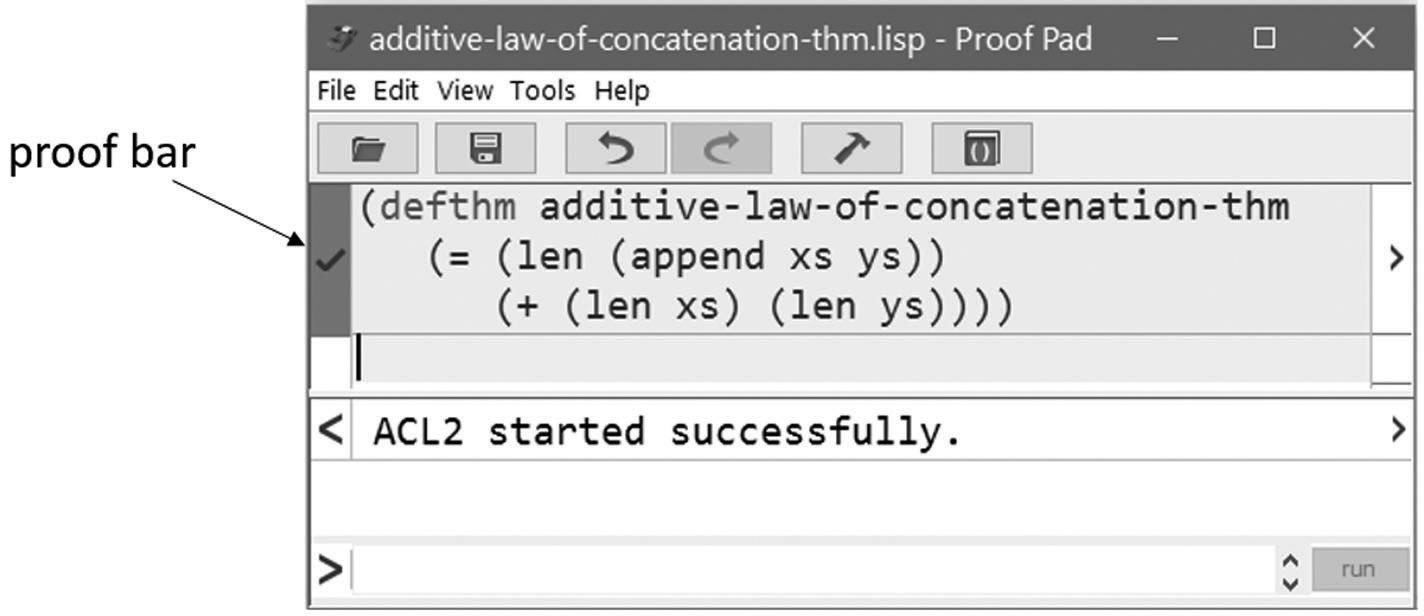
\includegraphics[scale=1]{images-cmyk/additive-law-of-concatenation-thm-acl2-prf-bw}
\end{center}
\index{Proof Pad!proof bar}\index{proof bar}
\caption{Proof Pad session with proof bar.}
\label{fig:proof-bar-with-chk}
\end{figure}

The mechanized logic of ACL2 fully automates the proof of this theorem.
It follows its own heuristic procedures to find an induction scheme
and pushes the proof through on its own.
To see ACL2 in action, enter the theorem into a Proof Pad session
and click in the green proof bar
(figure~\ref{fig:proof-bar-with-chk}, page \pageref{fig:proof-bar-with-chk}).
This sets ACL2 in motion to prove the theorem.
A check mark appears in the proof bar
when the mechanized logic succeeds.

\section{Using Books of Proven Theorems}
\label{sec:using-books-of-proven-theorems}

The append-suffix theorem states that
if the first operand of the \textsf{append} operator is a list of length $n$,
then dropping $n$ elements from the front of the concatenation
reproduces the second operand of \textsf{append}.
In section~\ref{sec:append-prefix-suffix} (page \pageref{append-suffix-thm-pencil-proof}),
we stated this theorem in the form ($\forall$$n$.S($n$)),
where S($n$) was a shorthand for the following equation:

\begin{samepage}
\begin{center}
S($n$) $\equiv$ $($\textsf{(nthcdr (len [$x_1$ $x_2$ $\dots$ $x_n$]) (append [$x_1$ $x_2$ \dots $x_n$] $ys$))}
$=$ $ys)$
\end{center}
\end{samepage}

In ACL2 notation, a definition of this theorem takes the following form:

\index{append!suffix theorem}\index{theorem!append-suffix}\index{theorem, by name!\{append-suffix\}}
\begin{code}
\begin{verbatim}
(defthm append-suffix-thm
  (equal (nthcdr (len xs) (append xs ys))
         ys))
\end{verbatim}
\end{code}

The mechanized logic can prove this theorem, but
the proof depends on some equations from numeric algebra.
Fortunately, ACL2 experts have already proved many such theorems,
and the ACL2 system makes them available in the form of
\index{book!ACL2}\seeonlyindex{ACL2 book}{book}\index{book!certified}\seeonlyindex{certified book}{book}``certified books''
(ACL2 terminology for a package of theorems successfully proven by the
mechanized logic).
A book known as
\index{book!arithmetic-3/top}\label{arith-top-book}\textsf{arithmetic-3/top}
contains theorems from algebra
\index{theorem!algebra, ACL2}that the mechanized logic can cite in
a proof of the append-suffix theorem.
An \textsf{include-book} directive tells ACL2 to
\index{directive!include-book}\index{directory (:dir)!:system}\index{system, :dir}\index{book!directory (:dir)}\seeonlyindex{import}{book}\index{theorem!import (\emph{see also} book)}import
these theorems.
\begin{code}
\begin{verbatim}
           (include-book "arithmetic-3/top" :dir :system)
\end{verbatim}
\end{code}

To make the theorems in the book available
for ACL2 to cite in a proof,
the directive precedes the \textsf{defthm} command that
defines the theorem to be proved, as shown in
figure~\ref{fig:append-suffix-acl2-prf} (page \pageref{fig:append-suffix-acl2-prf}).
Clicking in the proof bar sets the mechanized logic in motion,
and a check mark appears in the proof bar when
the proof is complete.
To try it for yourself in a Proof Pad session.
Enter the include-book directive
and theorem definition of figure~\ref{fig:append-suffix-acl2-prf},
click in the proof bar, and see what happens.

\begin{figure}
\begin{center}
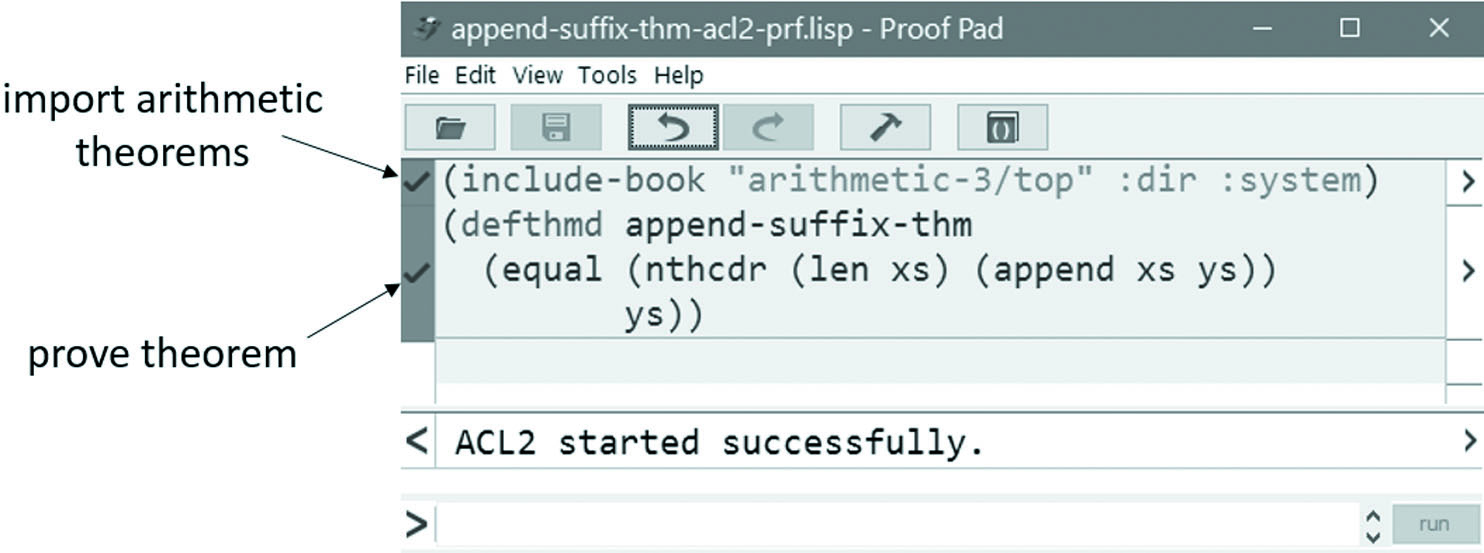
\includegraphics[scale=1]{images-cmyk/append-suffix-thm-acl2-prf-bw}
\end{center}
\index{theorem!append-suffix}\index{theorem, by name!\{append-suffix\}}\index{append!suffix theorem}
\caption{Append-Suffix: Importing theorems to cite in proof.}
\label{fig:append-suffix-acl2-prf}
\end{figure}

\begin{exercises}

\exer {Define the
\index{append!associative}\index{theorem!append associative}\index{theorem, by name!\{append associative\}}\index{associative}associativity property
of \textsf{append} (\{\emph{app-assoc}\}, page \pageref{app-assoc})
in ACL2 notation,
and use Proof Pad to run it through the ACL2 mechanized logic.
If you state the theorem correctly, ACL2 will succeed in proving it.\footnote{According
to \index{Moore, J Strother}J Strother Moore, a pioneer
in mechanized logic and a principal developer of ACL2,
the associativity of \textsf{append} was one of the driving examples in early work in
mechanized logic and one of the first theorems that such a system proved autonomously.}}

\exer {Define the following theorem in ACL2 and get the mechanized logic to prove it:\\
\hspace*{16mm}$\forall xs.($\textsf{(len (nthcdr (len xs) xs))} $=$ $0)$}

\end{exercises}

\section{Theorems with Constraints}
\label{sec:implies-constraints}

Another of the paper-and-pencil proofs in section~\ref{sec:append-prefix-suffix}
was the append-prefix theorem
(figure~\ref{numbered-list-interpretation}, page \pageref{numbered-list-interpretation}),
which referred to the prefix operator.

\begin{code}
\begin{verbatim}
(defun prefix (n xs)
   (if (and (posp n) (consp xs))
       (cons (first xs) (prefix (- n 1) (rest xs))) ; {pfx1}
       nil))                                        ; {pfx0}
\end{verbatim}
\end{code}

The append-prefix theorem, as stated for the paper-and-pencil proof,
had the form $\forall n.$S$(n)$,
where S($n$)
was written in terms of a numbered list.
The same theorem in ACL2 terminology uses a variable to designate the list.
~\\

Theorem \{append-prefix\} $\forall n.$S$(n)$

where S($n$) $\equiv$ $($\textsf{(nthcdr (len [$x_1$ $x_2$ $\dots$ $x_n$]) (append [$x_1$ $x_2$ $\dots$ $x_n$] $ys$))} $=$ $ys)$

\begin{code}
\begin{verbatim}
(defthm append-prefix-thm-NOT-QUITE-RIGHT
  (equal (prefix (len xs) (append xs ys))
         xs))
\end{verbatim}
\end{code}

However, the theorem as stated
is not quite correct,
and to explain why, we need to mention
some things we haven't told you about lists. A
\label{true-list-def}\index{true list}\index{list!true list}\emph{true list}
in ACL2 is either \textsf{nil} (the empty list)
or a value of the form \textsf{(cons $x$ $xs$)},
where $xs$ is a true list.
The predicate
\index{true-listp predicate}\index{predicate!true-listp}\textsf{true-listp}
is true when its operand
is a true list and false otherwise.

It can be verified by induction that
the \textsf{prefix} operator always delivers a true list.
The value \textsf{(prefix 0 $xs$)} is \textsf{nil}.
That takes care of the base case.
The value of \textsf{(prefix $(n+1)$ $xs$)} is either \textsf{nil}
(again, a true list)
or \textsf{(cons (first $xs$) (prefix $n$ (rest $xs$)))}.
We can assume by the induction hypothesis that
\textsf{(prefix $n$ (rest $xs$))} is a true list,
which means (by the definition of the term ``true list'')
that \textsf{(cons (first $xs$) (prefix $n$ (rest $xs$)))} is a true list.
That takes care of the inductive case and completes the proof
that \textsf{(prefix $n$ $xs$)} is always a true list.

When the second operand of \textsf{cons} is not a true list,
the value it constructs isn't a true list either.
For example, \textsf{(cons 2 1)} is not a true list because 1 is not a true list.
The formula \textsf{(cons 3 (cons 2 1))} also is not a true list,
again, because the second operand,
in this case \textsf{(cons 2 1)}, is not a true list.
However, \textsf{(len (cons 3 (cons 2 1))} is \textsf{2}, which you can work
out from the axioms or, easier,
just submit the formula to ACL2 and let it do the computation.
A similar computation reveals that
\textsf{(prefix (len (cons 3 (cons 2 1))) (cons 3 (cons 2 1)))}
is \textsf{(cons 3 (cons 2 nil))}, not \textsf{(cons 3 (cons 2 1))}.
That is, when $xs$ is \textsf{(cons 3 (cons 2 1))},
then \textsf{(prefix (len $xs$) (append $xs$ $ys$))} is not equal to $xs$.
The equation that theorem append-prefix-thm-NOT-QUITE-RIGHT
guarantees does not hold when $xs$ is \textsf{(cons 3 (cons 2 1))}.
Since a theorem cannot have exceptions,
the theorem append-prefix-thm-NOT-QUITE-RIGHT
isn't true.

\begin{aside}{thm-with-implies}{Using Implication to Constrain the Domain of a Theorem}
A theorem that takes the form of an implication, $x \rightarrow y$,
says that the conclusion, $y$, will be true when the hypothesis, $x$,
is true, but it says nothing about the status of the conclusion when
the hypothesis is false. The ACL2 equivalent of the Boolean formula $x \rightarrow y$
is \textsf{(implies $x$ $y$)}.
For example, one can conclude that $u - 1 < v - 1$
if one knows that $u < v$.
In ACL2, this fact would be stated as an implication.
\begin{code}
\begin{verbatim}
(defthm simple-theorem-about-numbers
  (implies (< u v)
           (< (- u 1) (- v 1))))
\end{verbatim}
\end{code}\index{theorem!constraints}\index{theorem!implication, constraint}
%\caption{Using Implication to Constrain the Domain of a Theorem}
%\label{thm-with-implies}
\end{aside}

The theorem is true, however, when the variable $xs$ is
constrained to the domain of true lists.
In the statement of the append-prefix theorem in
section~\ref{sec:append-prefix-suffix} (page \pageref{append-prefix-thm-predicate}),
the role of $xs$ was played by the numbered list
\textsf{[$x_1$ $x_2$ $\dots$ $x_n$]},
which is a true list by definition
(page \pageref{numbered-list-interpretation}).
ACL2 does not permit the use of the numbered list syntax,
so the true-list constraint must be explicit.
An implication formula imposes the necessary constraint.

\begin{code}
\begin{verbatim}
(defthm append-prefix-thm
   (implies (true-listp xs)
            (equal (prefix (len xs) (append xs ys))
                   xs)))
\end{verbatim}
\end{code}

\begin{figure}
\begin{center}
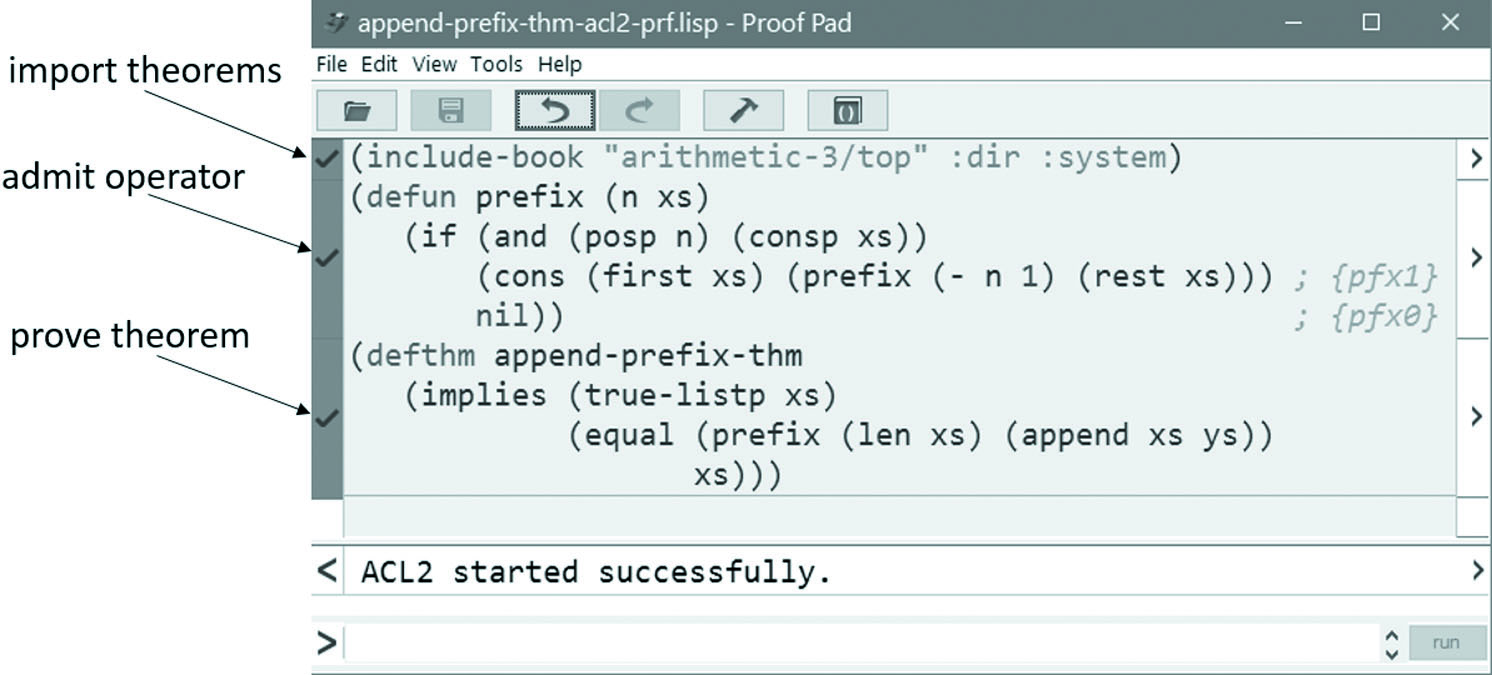
\includegraphics[scale=1]{images-cmyk/append-prefix-thm-acl2-prf-bw}
\end{center}
\index{append!prefix theorem}\index{theorem!append-prefix}
\index{theorem, by name!\{append-prefix\}}
\caption{Append-Prefix theorem: an implication.}
\label{fig:append-prefix-acl2-prf}
\end{figure}

Now we have a theorem that we believe is true
based on our paper-and-pencil proof.
The mechanized logic of ACL2
succeeds in proving this theorem, but, as was the case with
the append-suffix theorem
(figure~\ref{fig:append-suffix-acl2-prf}, page \pageref{fig:append-suffix-acl2-prf}),
it needs to cite some theorems of numeric algebra.
Figure~\ref{fig:append-prefix-acl2-prf} (page \pageref{fig:append-prefix-acl2-prf})
displays a Proof Pad session that imports those theorems,
defines the prefix operator, and then states and proves the theorem.
The figure indicates that ACL2
\index{admit, ACL2}\index{ACL2!admit}``admits''
the prefix operator when it encounters its definition.
This means that ACL2 allows the definition to join
the universe of entities that can participate in
the mechanized reasoning process.
Box~\ref{reason-for-acl2-admit} (page \pageref{reason-for-acl2-admit})
explains what this entails.

\begin{aside}{reason-for-acl2-admit}{ACL2 Must Prove That Operators Terminate}
In figure~\ref{fig:append-prefix-acl2-prf},
there is a step that has the label ``admit operator.''
That is the terminology ACL2 uses for the process of accepting
an operator into its mechanized logic.
A domain in which operators may fail to terminate
calls for a more complex reasoning process than a domain that is
restricted to operators that are guaranteed to complete their
computation in a finite number of steps.
To give itself a better shot at succeeding in mechanized proofs,
ACL2 does not deal with operators with a potential for nontermination.
It will \emph{admit} an operator to its domain of logic
only if it can verify termination in all cases.
Sometimes, coming up with an operator definition that makes
it possible for ACL2 prove termination is, by itself,
a major project, including importing theorems or coming up with new
theorems to facilitate the reasoning process.
Hardware and software with guaranteed properties are not easy to come
by.\index{admit, ACL2}\index{ACL2!admit}
%\caption{ACL2 Must Prove That Operators Terminate}
%\label{reason-for-acl2-admit}
\end{aside}

\begin{exercises}

\exer {Define the \{\emph{rep-len}\} theorem (page \pageref{rep-len}) in ACL2,
and use Proof Pad to run it through the mechanized logic.
(\emph{Hint}: Use \textsf{natp} to constrain the first operand of \textsf{rep}.)}

\exer {An exercise in section~\ref{sec:append-prefix-suffix} required a paper-and-pencil
proof of the following proposition: $\forall xs.($\textsf{(nthcdr (len $xs$) $xs$)} $=$ \textsf{nil}$)$.
Define this theorem in ACL2 and get the mechanized logic to prove it.}

\exer {The formula \textsf{(equal (prefix (len $xs$) $xs$) $xs$)} is true with a certain
constraint on $xs$. Define an ACL2 theorem with this equation as its conclusion
and get the mechanized logic to prove it.}

\end{exercises}

\section{Helping Mechanized Logic Find Its Way}
\label{sec:lemmas}

The mechanized logic of ACL2 was able to carry out proofs of
the theorems of section~\ref{sec:theorems-and-acl2-proofs} without assistance.
To prove the theorems in Section~\ref{sec:using-books-of-proven-theorems},
ACL2 needed to cite some proven theorems packaged in books
developed by experts.
These were carefully chosen examples to get started with
the mechanized proofs.
Usually, the process of using a mechanized logic requires
both proven theorems packaged in books
and specialized theorems chosen to match the
needs of a particular goal.
That is, to succeed in proving a complex property of
an operator defined in ACL2,
it is usually necessary to prove
some simpler properties that the mechanized
logic can cite in a proof of the more complex property.

\index{ACL2!helping}Choosing simpler properties that ACL2 can prove
and building, finally, to the more complex proof
calls for insight and creativity.
This is where your experience with paper-and-pencil proofs
comes in handy.
You can plan a strategy by thinking of major steps
in a proof, stating those steps as separate theorems,
and proving them one by one to build up a body
of helpful theorems that the mechanized logic
can cite to move closer to the goal.

It may help to see an example of how this can work.
The Fibonacci numbers are a well-studied sequence that
scientists have used to study
patterns of development in leaves and flowers,
growth rates in animal populations,
and other natural phenomena.
The sequence can be defined inductively
with the Fibonacci equations
(figure~\ref{fig:Fibonacci-axioms}, page \pageref{fig:Fibonacci-axioms}).

\begin{figure}
\begin{center}
Axioms \{\emph{Fibonacci}\}
\begin{tabular}{ll}
$f_0$ $=$ $0$                   & \{\emph{f0}\} \\
$f_1$ $=$ $1$                   & \{\emph{f1}\} \\
$f_{n+2}$ $=$ $f_{n+1} + f_{n}$ & \{\emph{f2}\} \\
\end{tabular}
\begin{code}
\begin{verbatim}
(defun fib(n) ; n-th Fibonacci number
  (if (posp (- n 1))                      ; n > 1
      (+ (fib(- n 1)) (fib(- n 2)))       ; {fib2}
      n))                                 ; {fib1}
\end{verbatim}
\end{code}

\begin{tabular}{llllllllll}
\dots & \textsf{(fib 2)} & \textsf{(fib 3)} & \textsf{(fib 4)} & \textsf{(fib 5)} & \dots & \textsf{(fib 10)} & \textsf{(fib 11)} & \textsf{(fib 12)} & \dots \\
\dots & ~~~~~1  &  ~~~~2  &  ~~~~3  &  ~~~~5  & \dots &  ~~~~~55 &  ~~~~~89 & ~~~144   & \dots \\
\end{tabular}
\end{center}
\index{Fibonacci!numbers}\index{axiom!Fibonacci}\index{operator, by name!fib, fib-fast (Fibonacci)}\index{Fibonacci!operator}\index{equation, by name!\{f0\}, \{f1\}, \{f2\}}\index{equation, by name!\{fib1\}, \{fib2\}}\index{axiom, by name!\{f0\}, \{f1\}, \{f2\}}
\caption{Fibonacci numbers.}
\label{fig:Fibonacci-axioms}
\end{figure}

The Fibonacci operator, \textsf{fib}, defined in ACL2,
mirrors the algebraic equations.
It selects the inductive formula
\textsf{(fib$(n - 1)$) + (fib$(n - 2)$)}
for an operand $n$ that is 2 or bigger
(that is, when $(n-1)$ is a positive, natural number).
For smaller operands, the ACL2 definition
observes that the corresponding Fibonacci number
is the same as the operand:
\textsf{(fib 0)} $=$ $f_0$ $=$ $0$ by axiom \{\emph{f0}\}
and \textsf{(fib 1)} $=$ $f_1$ $=$ $1$ by axiom \{\emph{f1}\}.

We can be confident that $\forall n.($\textsf{(fib $n$)} $=$ $f_n)$
because the ACL2 definition of \textsf{fib} is a direct
transliteration of the Fibonacci equations.
We can use the operator \textsf{fib} as a calculator
to compute some Fibonacci numbers.
This works well for small numbers, but it turns out that there are
a huge number of computational steps required to derive
\textsf{(fib $n$)} from the Fibonacci axioms when $n$ gets above a few dozen.
For example, the computation of \textsf{(fib 30)} proceeds quickly,
but you will see a noticeable delay if you ask ACL2 to compute \textsf{(fib 40)},
and you would have to wait a long time for \textsf{(fib 50)}.

It's not to hard to see the reason for this.
The axioms calculate \textsf{(fib $(n+2)$)} by first calculating
(\textsf{fib $(n+1)$)}, then calculating \textsf{(fib $n$)}, and finally
adding those two numbers together.
However many computational steps it takes to compute \textsf{(fib $n$)},
it will take at least a few more to compute \textsf{(fib $(n+1)$)}.
So, there will be more than twice as many steps in the computation of \textsf{(fib $(n+2)$)}
as there are in the computation of \textsf{(fib $n$)}.
That is, when $n$ increases by 2, the number of computational steps more than doubles.

If we let $c_n$ stand for the number of computational steps in the calculation
of \textsf{(fib $n$)}, then our observation about doubling amounts to the
inductive relationship $c_{n+2} \geq 2c_n$.
We think you have had enough experience to prove (by induction, of course)
that $\forall n.(c_{2n+1} \geq 2^n)$,
assuming that it takes at least one computational step to compute \textsf{(fib $1$)}.
That's what they call \emph{exponential growth}.\footnote{The term
``exponential growth'' is bandied about a lot, but mostly
in ways that do not match the standard mathematical meaning.
The most common usage is to describe something that
gets big fast, which is certainly true of exponential growth,
but it is also true of quadratic growth.
Quadratic growth often gets passed off, informally, as exponential growth,
but it's not even close. If the number of computational steps
in computing \textsf{(fib $n$)} from the axioms grew quadratically instead of exponentially,
it would not take a lot longer to compute \textsf{(fib 40)} than it does to compute \textsf{(fib 30)}.}
It is dramatic, to say the least. We estimate that it would take an hour to compute
\textsf{(fib 50)} on a typical laptop computer and upwards of a year to compute \textsf{(fib 75)}.

The Fibonacci axioms comprise an
\index{Fibonacci!definition}inductive definition.
They conform to the three C's
(figure~\ref{fig:inductive-def-keys}, page \pageref{fig:inductive-def-keys}),
so they guarantee delivery of a Fibonacci number
in a finite number of computational steps.
Unfortunately, in this case it turns out to be
a huge number of computational steps.
Fortunately, there are alternatives.

If a particular inductive definition leads to a long computation,
there may be another inductive definition that produces the same
results with less work,
and that is the case with Fibonacci numbers.
Figure~\ref{fig:gib-defun} (page \pageref{fig:gib-defun})
displays another definition that uses a method known as
\index{tail recursion}\index{definition!tail recursive}\emph{tail recursion}.\footnote{\index{recursive}``Recursive definition''
is the most commonly used term for what we call ``inductive definition.''
We don't say ``recursive'' because the term is often conflated
with a computation strategy based on a data structure called a stack,
and we think fixating on computational detail obscures the meaning
of the definition.
We want you to think of inductive (aka recursive)
definitions as axiomatic equations that can be used to reason about the
operators they define. We leave it to the computer system
to determine how to carry out the computation.
Sometimes, as in the Fibonacci problem
where an inductive definition leads to inefficient computation,
we will look for more efficient alternatives,
but we will not relinquish our view of operator definitions
as axioms to support reasoning. If our programming language allowed
mutable variables, as most programming languages do, we would
delve into a stack-based view of recursion.
Since it doesn't, we won't.}
A tail recursion is a circular reference in an operator definition
that occurs at the
\index{top level, vs nested}\index{nested, vs top level}\emph{top level},
which means that it is not nested
inside a formula to produce an operand for another operator.
The operator \textsf{h} occurs at the top level
in the formula \textsf{(h (+ $x$ 1))},
but it is nested in the formula \textsf{(+ (h $x$) 1)}.
Most computing systems, including ACL2,
implement tail recursions efficiently. Nested recursions are
more problematic. They don't always lead to inefficient computations,
but sometimes, as with Fibonacci numbers, they do.

\begin{figure}
\begin{center}
\begin{code}
\begin{verbatim}
(defun gib (n b a)  ; b = (fib(n-1)), a=(fib(n-2))
   (if (posp (- n 1))
       (gib (- n 1) (+ b a) b)            ; {gib2}
       (if (= n 1)
           b                              ; {gib1}
           a)))                           ; {gib0}
(defun fib-fast (n) ; (fib-fast n)=(fib n)
   (gib n 1 0))     ; (fib 1)=1, (fib 0)=0
\end{verbatim}
\end{code}
\end{center}
\seeonlyindex{fib, fib-fast}{operator}\index{Fibonacci!fast}\index{Fibonacci!operator}\index{operator, by name!fib, fib-fast (Fibonacci)}\index{operator, by name!gib (iterative Fibonacci)}\index{equation, by name!\{gib0\}, \{gib1\}, \{gib2\}}\index{gib (\emph{see also} operator)}
\caption{Fibonacci numbers: quick delivery.}
\label{fig:gib-defun}
\end{figure}

The downside is that \index{tail recursion!reasoning about}\index{reasoning!about tail recursion}reasoning
about tail recursive
definitions is often more challenging than reasoning about definitions
with nested recursions. One way to proceed, however,
is to define an operator both ways, prove that the two definitions
produce the same results, and then use the efficient definition
for computation and the inefficient one when it
simplifies the reasoning process.

If you look at the definition of \textsf{fib-fast} (figure~\ref{fig:gib-defun})
closely, we think you will agree that, although it may seem plausible
that \textsf{(gib $n$ $1$ $0$)} is the $n^\textnormal{th}$ Fibonacci number,
it isn't obvious.
Some reasoning is required.
Maybe ACL2 can take it on successfully.
We would like to know that $\forall n.($\textsf{(fib-fast $n$)} $=$ \textsf{(fib $n$)}$)$.
The theorem in ACL2 terms can be stated as follows:
\index{theorem, by name!\{fib=fib-fast\}}\index{Fibonacci!fast}\index{theorem!Fibonacci fast}
\begin{center}
\begin{code}
\begin{verbatim}
(defthm fib=fib-fast ; (fib-fast n) = (fib n)
    (implies (natp n)
             (= (fib n) (fib-fast n))))
\end{verbatim}
\end{code}
\end{center}

When ACL2 tried to prove this theorem it failed,
or at least it took such a long time floundering that we interrupted it
to try something else.
We thought maybe it needed to know some theorems from numeric
algebra, so we imported the arithmetic-3/top book, as usual,
but that didn't help. It still sat there spinning,
so we interrupted it again.

We guessed that it might be having trouble coming up with an effective
induction hypothesis, so we decided to ask it to prove that
the \textsf{gib} operator satisfies the basic Fibonacci axioms.
This is, to prove that the $n^\textnormal{th}$ value of \textsf{gib} is
the sum of the previous two values (as in axiom \{\emph{f2}\}).
In ACL2, that theorem can be stated as follows:
\index{gib (\emph{see also} operator)}\index{theorem!gib lemmas (base, inductive)}\index{gib (\emph{see also} operator)!lemmas (base, inductive)}
\begin{center}
\begin{code}
\begin{verbatim}
(defthm gib-inductive-equation ; a la {fib2}
    (implies (posp (- n 1))              ; n > 1
             (= (gib n b a)              ; n-th
                (+ (gib (- n 1) b a)     ; (n-1)th
                   (gib (- n 2) b a))))) ; (n-2)th
\end{verbatim}
\end{code}
\end{center}

ACL2 failed quickly this time and reported that it was not able
to find an induction scheme that worked.
So, our attempt to help ACL2 along didn't work, exactly, %'
but at least ACL2 could determine quickly that
things were not going well.
Next, we guessed that ACL2 might need help with the
base case as well as the inductive case, so we
stated a base case for the \textsf{gib} operator as an ACL2 theorem.
\index{theorem!gib lemmas (base, inductive)}\index{gib (\emph{see also} operator)!lemmas (base, inductive)}
\begin{center}
\begin{code}
\begin{verbatim}
(defthm gib-base-equation ; a la {fib1}
    (= (gib 1 b a) b))
\end{verbatim}
\end{code}
\end{center}

This idea worked. ACL2 was able to prove the gib base equation
and the gib inductive equation, and then finally
used them to prove that $\forall n.($\textsf{(fib-fast $n$)} $=$ \textsf{(fib $n$)}$)$,
in the form defined in the \textsf{fib=fib-fast} theorem.
Figure~\ref{fig:fib-gib-thm} (page \pageref{fig:fib-gib-thm})
displays the Proof Pad session with the check-marks
indicating completed proofs by the mechanized logic of ACL2.
Try out the \textsf{fib-fast} operator in a Proof Pad session.
The Fibonacci number \textsf{(fib-fast $n$)} seems to appear
instantaneously, even for large values of $n$.

\begin{figure}
\begin{center}
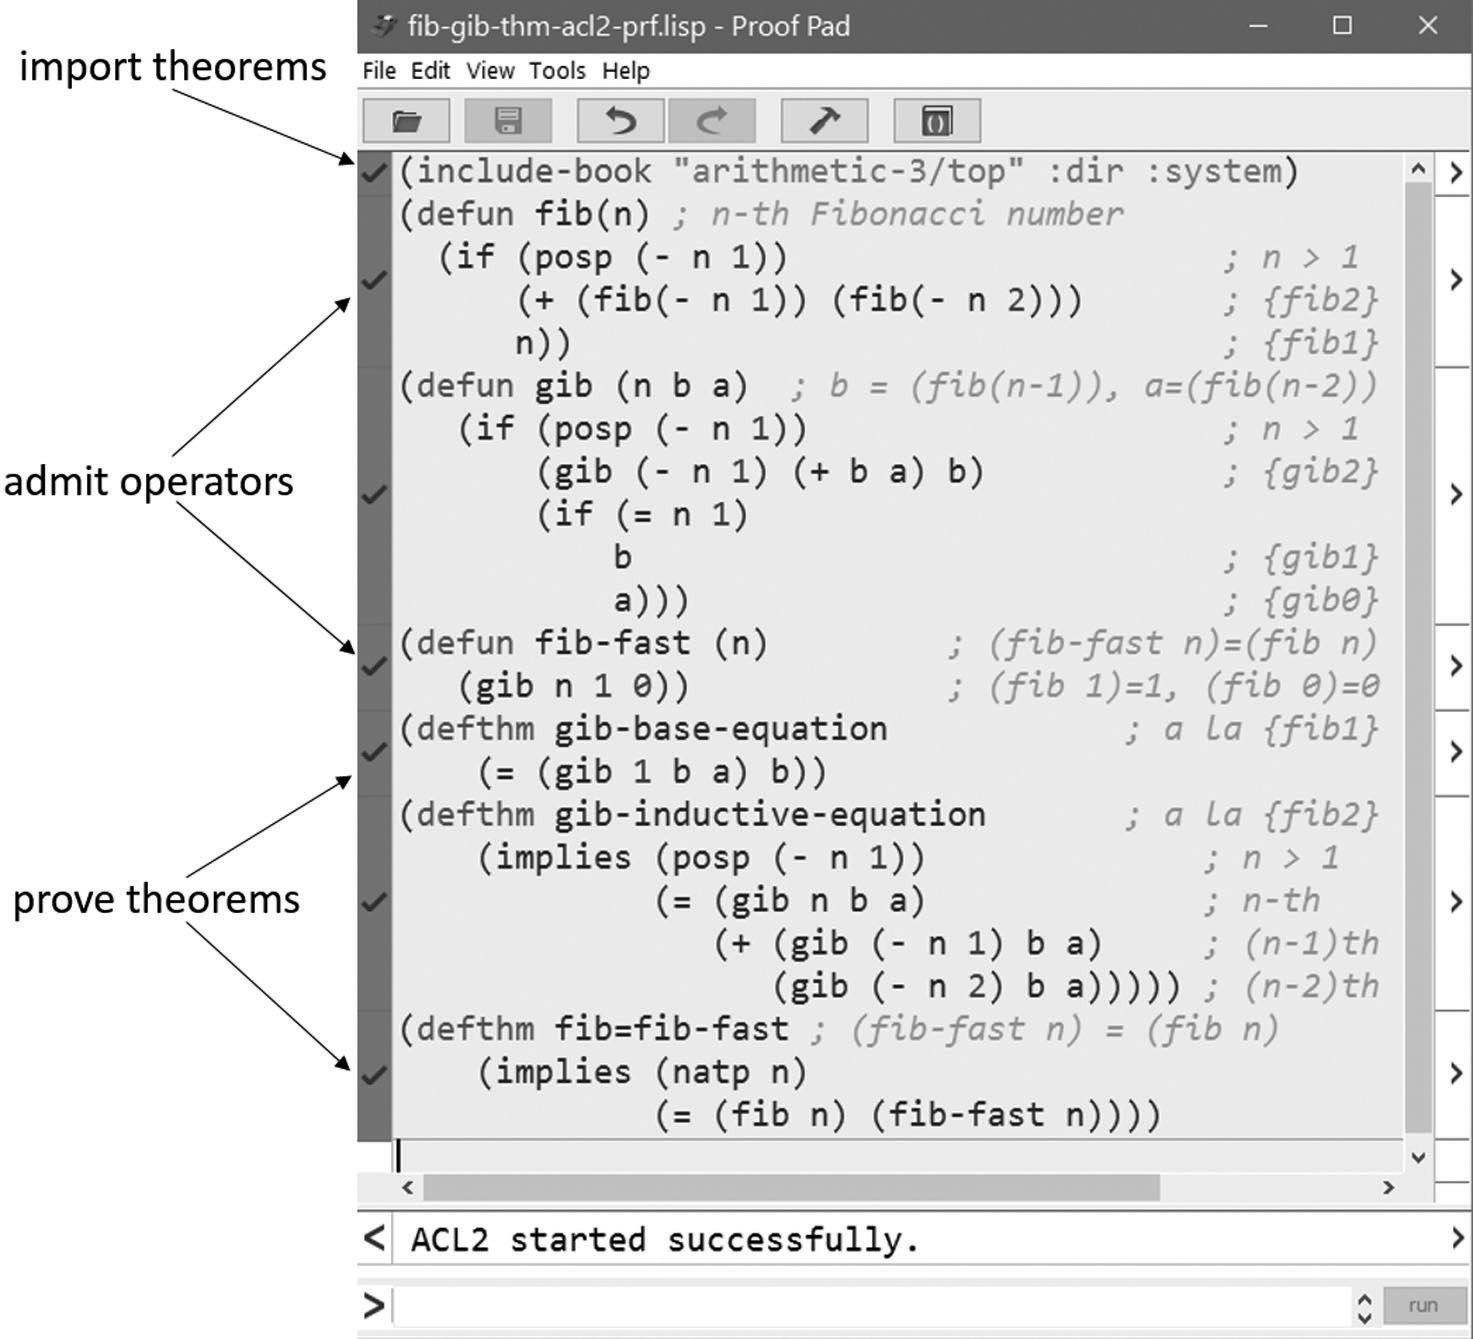
\includegraphics[scale=1]{images-cmyk/fib-gib-thm-acl2-prf}
\end{center}
\caption{Fast Fibonacci delivers Fibonacci numbers.}
\label{fig:fib-gib-thm}
\end{figure}

\begin{exercises}

\exer {Assume that $c_1 = 1$ and $c_{n+2} = 2c_n$.
Prove that $\forall n.(c_{2n+1} = 2^n)$.\\
\emph{Hint}: Define $x_n = c_{2n+1}$.
First, verify that $x_{n+1} = 2x_n$.
Then, use mathematical induction to prove that $x_n = 2^n$,
and translate this formula for $x_n$
to a formula for $c_{2n+1}$.\\
\index{exponents, law of}\emph{Note}: $2^0 = 1$, $\forall n.(2^{n+1} = 2 \times 2^n)$ \{\emph{Law of Exponents}\}}

\end{exercises}

\section{Proof Automation and Things That Can't Be Done}
\label{sec:halting-problem}

By now you've had some experience constructing proofs, and if you're like most people,
it has been tough going most of the time.
It's rarely easy to figure out how to prove a theorem,
and it's often extraordinarily difficult.
How is it, then, that a mechanized logic like ACL2 can succeed at such a difficult task?
How does ACL2 prove theorems?

First of all, it doesn't, most of the time.
Our examples have been carefully constructed in a way that
led to success by ACL2.
If you try on your own to propose theorems
and present them to ACL2 for proof, you will find that it can be
extremely difficult to get ACL2 to succeed, even with a lot of help.
Often, you will need to sketch a proof yourself,
then give ACL2 a sequence of smaller theorems
that it can prove, one by one, building up to
the theorem that was your goal in the first place,
with plenty of roadblocks and changes in strategy along the way.

Even when all ACL2 has to do is fill in a few gaps,
we find it remarkable that ACL2 can succeed in proving theorems.
And it \emph{is} remarkable.
When researchers began trying to automate parts
of the theorem-proving process, it was many years
before really effective tools began to emerge.
Now, mechanized logic plays a role in
the verification of important properties of digital circuits and
software, not only in research labs
but also in engineering projects with deadlines and product cycles.
And it's not just ACL2. Many systems of mechanized logic %'
have been developed over the past half-century or so
by distinguished researchers in the USA, the UK, France, Sweden, and elsewhere.

\begin{aside}{mechanized-logic-history}{Mechanized Logics: Fifty Years of R\&D, Mostly R}
\begin{itemize}
\item ACL2 (and precursor nqthm): J Moore, Robert Boyer, and Matt Kaufmann, University of Texas, with a long history starting at the University of Edinburgh and continuing at Xerox PARC and SRI
\item LCF, HOL, Isabelle: Robin Milner, Mike Gordon, Lawrence Paulson, Stanford University, Cambridge University, University of Edinburgh
\item Coq: Thierry Coquand, G\'erard Huet, INRIA, University of Gothenburg
\item PVS: Sam Owre, Natarajan Shankar, John Rushby, SRI
\item Agda: Ulf Norell, Chalmers University
\item LF: Robert Harper, Furio Honsell, Gordon Plotkin, Carnegie Mellon University, University of Udine, University of Edinburgh
\item Twelf: Frank Pfenning, Carsten Sch\"urmann, Carnegie Mellon University, University of Copenhagen
\end{itemize}\index{logic!mechanized}\index{Twelf}\index{Pfenning!Frank}\index{Sch\"urmann, Carsten}\index{LF}\index{Harper, Robert}\index{Honsell, Furio}\index{Plotkin, Gordon}\index{Agda}\index{Norell, Ulf}\index{PVS}\index{Owre, sam}\index{Natarajan, Shankar}\index{Rushby, John}\index{Coq}\index{Coquand, Thierry}\index{Huet, G\'erard}\index{LCF}\index{HOL}\index{Isabelle}\index{Milner, Robert}\index{Gordon, Mike}\index{Paulson, Lawrence}\index{ACL2}\index{Moore, J Strother}\index{Boyer, Robert}\index{Kaufmann, Matt}
%\caption{Mechanized Logics: Fifty Years of R\&D, Mostly R}
%\label{mechanized-logic-history}
\end{aside}

Proofs are not only hard.
They are sometimes impossible, as G\"odel famously proved in 1931,
to the great surprise of many mathematicians of the day.
In the same vein, there are things computers cannot do.
A well-known example is the \index{halting problem}\emph{halting problem}, which
was proved to be outside the realm of computation
by \index{Turing, Alan}Alan Turing in 1936
and, independently, by \index{Church, Alonzo}Alonzo Church.
There were no computers at the time,
but there were mathematical models of computation
that are used still today to study the capabilities of computers.

A program solving the
\index{uncomputable}\index{halting problem}halting problem would be able to determine,
given a computer program, whether or not the program would terminate
in a finite amount of time given a particular input.
There are programs that can solve the halting problem for
a limited set of programs,
but no program can solve the halting problem for all programs.
Proving that no computer program can solve the halting problem is tricky,
but the ideas are not too difficult to follow, and
they provide an example of reasoning that,
in a perverse sense, fits into a discussion of mechanized logic
because it exhibits something that neither computers
nor people can do. There are many such things, as a search
on the term ``uncomputable'' shows.

To be specific, the following discussion of the halting problem
limits itself to a single programming language, but
that restriction turns out to be immaterial.\footnote{The
halting problem cannot be solved
for any ``general purpose'' \index{programming language}programming language,
by which we mean a \index{Turing complete}Turing complete language,
which itself calls for a long explanation even
before discussing how Turing completeness
interacts with the halting problem.
You can track that down if you're interested.
All widely-used programming languages
(\index{ACL2}ACL2, \index{Java}Java, and \index{C++}C++, for example) are \index{Turing complete}Turing complete.
We'll leave it at that.}
Because discussion of the halting problem is clumsy in ACL2,
we'll present the ideas in terms of a different
language that has the same syntax
and a similar interpretation. That language is Lisp.
For the purposes of this discussion,
you can think of Lisp as ACL2 with the added feature
of allowing operators to act as operands.
That is, a formula invoking an operator can supply
another operator as input.
Most programming languages allow this.
ACL2 doesn't because the extra facility
interferes with some of the strategies that ACL2 uses
to mechanize the process of proving theorems.

The discussion will include some logic formulas with
quantification,
so we need to specify the universe of discourse
(page \pageref{def-universe-of-discourse}).
When the bound variable
in the formula is $h$, the universe of discourse
will be the set of operators that have
two operands and can be defined in Lisp:
\textsf{(defun $h$ ($f$ $x$)} $\dots$ \emph{Lisp formula} $\dots$ \textsf{)}.
When the bound variable is $f$,
the universe of discourse will be the set of operators
that have one operand and can be defined in Lisp:
\textsf{(defun $f$ ($x$)} $\dots$ \emph{Lisp formula} $\dots$ \textsf{)}.\footnote{The
restriction to one operand simplifies the presentation,
but it is not really a restriction because the operand could
be a list containing any number of values.}
When the bound variable is $x$, the universe of discourse
is the set of values that Lisp operators can deliver.

We define a predicate, $H$, that tells us whether or not
a particular formula in Lisp represents a computation that terminates,
that is, a computation that would be completed in a finite amount of time.
$H$ is not a Lisp operator and does not itself
represent a computation. It is a mathematical entity
outside the realm of computation that gives us a way
to use symbols and formulas to talk about
whether or not a computation terminates.

The definition of the predicate $H$ uses the Lisp
formula \textsf{($f$ $x$)} to designate a computation that may
or may not be completed in a finite amount of time.
Since $H$ is a logic predicate, not a computation,
it has a value whether or not the formula \textsf{($f$ $x$)} terminates.

%\begin{quote}
\index{predicate, by name!H (termination)}\index{termination predicate (H)}
\label{def:predicate-H}
\hspace*{5mm}\emph{Definition of predicate} $H$:\\
\hspace*{10mm}$H(f, x) = True$, if \textsf{($f$ $x$)} terminates\\
\hspace*{10mm}$H(f, x) = False$, if \textsf{($f$ $x$)} does not terminate
%\end{quote}

The theorem that Turing and Church proved is that
no operator $h$ can be defined in Lisp
that accepts a Lisp operator $f$ as its
first operand and a Lisp value $x$ as its second operand
such that, regardless of the definition of the operator $f$,
\textsf{($h$ $f$ $x$)} $=$ 0 if the computation \textsf{($f$ $x$)} terminates and
\textsf{($h$ $f$ $x$)} $=$ 1 if \textsf{($f$ $x$)} does not terminate.
This means not just that it would be hard to define the operator $h$.
It means that nobody can define $h$ with any amount of effort or cleverness.
There is no such definition.
There are some things that cannot be done, and this is one of them.

\label{church-turing-hypothesis}\index{Church--Turing hypothesis}\index{Turing--Church hypothesis}\index{hypothesis!Church--Turing}A
conjecture of Church and Turing
concerning the effectiveness of general-purpose programming languages
asserts that for any computation that can be carried out, there is a program
that can be written in Lisp (or any other general-purpose programming language)
that specifies a way to carry out the computation.
If one believes Church--Turing conjecture, and most computer scientists do,
then the theorem that Church and Turing proved about the prospects of
automating the prediction of program termination
says that no program can be written that solves the halting problem.
Neither Turing nor Church stated the theorem in terms of Lisp.
Turing used a model of computation known as the Turing machine, and
Church used the lambda calculus, another model of computation.
Both models are still widely studied in computer science theory,
and the programming language Lisp
was based on the lambda calculus.

We express the \index{halting problem}halting problem
theorem as a logic formula that we will prove
using natural deduction (section \ref{sec:deduction}).
The theorem has no hypotheses.
\vspace{2mm}\\
%\begin{quote}
\index{theorem!halting problem}\index{theorem, by name!\{halting problem\}}
\hspace*{5mm}Theorem \{halting problem\}:\\
\hspace*{1cm}$\vdash$ $\neg(\exists h. \forall f. \forall x.
((H(f, x) \rightarrow ($\textsf{($h$ $f$ $x$)} $=$ $1)) \wedge ((\neg H(f, x)) \rightarrow ($\textsf{($h$ $f$ $x$)} $=$ $0))))$
\vspace{2mm}
%\end{quote}

There are two Lisp formulas embedded in
the logic formula of the theorem, both the same:
\textsf{($h$ $f$ $x$)}.
Those formulas invoke an operator $h$, which is defined in Lisp because that is the universe
of discourse for $h$, the bound variable in the $\exists$ quantification.
The logic formula then compares the value that
the formula \textsf{($h$ $f$ $x$)} computes to a natural number.

To make the proof more compact and, we hope, more readable,
we will use $E$ as an abbreviation for the
long $\exists$ formula whose negation is the conclusion of the theorem.
\vspace{2mm}\\
%\begin{quote}
\hspace*{5mm}$E$ $\equiv$ $\exists h. \forall f. \forall x.
((H(f, x) \rightarrow ($\textsf{($h$ $f$ $x$)} $=$ $1)) \wedge ((\neg H(f, x)) \rightarrow ($\textsf{($h$ $f$ $x$)} $=$ $0)))$
\vspace{2mm}
%\end{quote}

With the abbreviation, the \{halting problem\} theorem is: $\vdash$ $\neg E$.
Figure~\ref{fig:halting-proof-strategy} (page \pageref{fig:halting-proof-strategy})
displays the proof, which uses the natural deduction formalism.
It cites a theorem we already proved, theorem \{$\neg \neg$ forward\}, and
a theorem, \{paradox\}, which we will prove
after showing how our goal, the \{halting problem\} theorem,
can be derived from it.
To clarify the derivation, we need to state the \{paradox\} theorem,
which we will prove later.
\vspace{2mm}\\
%\begin{quote}
\index{theorem!paradox}\index{theorem, by name!\{paradox\}}\index{paradox, halting problem}\index{halting problem}
\hspace*{5mm}Theorem \{paradox\}: $E$ $\vdash$ $False$
\vspace{2mm}
%\end{quote}

In addition to citing the \{paradox\} theorem,
the proof of the \{halting problem\} theorem
cites the \{reductio ad absurdum\} inference rule
(figure~\ref{fig-02-deduction-rules}, page \pageref{fig-02-deduction-rules}),
so our proof of the \{halting problem\} theorem is a proof by contradiction.
It begins by assuming the negation of the formula in its conclusion.
The assumption, as always, stands in lieu of a proof.
As it happens, the assumption is discharged later in the proof,
leaving the \{halting problem\} theorem with no hypotheses,
as it is stated.
The conclusion of the theorem is the negation of a long there-exists formula.
What this means is that there is no program that, 
given an arbitrary program \emph{p}, can
determine in a finite number of computation steps
whether the program \emph{p} will terminate.

\begin{figure}
Theorem \{halting problem\}: $\vdash$ $\neg E$ ~~~~~~~~\emph{Note: This theorem has no hypotheses.}\\
\hspace*{5mm}where $E$ $\equiv$ $\exists h. \forall f. \forall x.
((H(f, x) \rightarrow ($\textsf{($h$ $f$ $x$)} $=$ $1)) \wedge ((\neg H(f, x)) \rightarrow ($\textsf{($h$ $f$ $x$)} $=$ $0)))$)\\
proof
\begin{center}
\begin{tabular}{ll}
Assume $(\neg(\neg E))$                       &\emph{this assumption will discharged}\\
------------------------\{$\neg \neg$ forward\} &\emph{proved in figure~\ref{fig:dbl-neg-fwd} (page \pageref{fig:dbl-neg-fwd})}\\
~~~~~~~~~~~~$E$                               &\\
------------------------\{paradox\}           &\emph{proved in figure~\ref{fig:proof-paradox-thm} (page \pageref{fig:proof-paradox-thm})}\\
~~~~~~~~$False$                               &\\
------------------------\{$\rightarrow$ introduction\} &\emph{assumed} $(\neg(\neg E))$\emph{, proved} $False$\emph{,}\\
~~$(\neg(\neg E)) \rightarrow False$          &~~~~\emph{conclude} $(\neg(\neg E)) \rightarrow False$\\
Discharge $(\neg(\neg E))$                    &\emph{this discharge leaves no hypotheses}\\
------------------------\{reductio ad absurdum\}&\emph{figure~\ref{fig-02-deduction-rules} (page \pageref{fig-02-deduction-rules})}\\
~~~~~~~~~~~$\neg E$                           &\\
\end{tabular}
\end{center}
\index{halting problem}\index{theorem!halting problem}\index{theorem, by name!\{halting problem\}}
\caption{Theorem \{halting problem\}: a proof by contradiction.}
\label{fig:halting-proof-strategy}
\end{figure}

We are not quite ready to tackle the \{paradox\} theorem.
The proof will be easier to follow if we break it into parts,
then connect the parts in the final analysis.

Recall that $E$, the hypothesis of the \{paradox\} theorem,
is a $\exists$ formula.
Since $E$ is a hypothesis of the \{paradox\} theorem,
we will assume at the beginning of the proof
of the \{paradox\} theorem that $E$ is true.
$E$ asserts that there is at least one definition of
an operator $h$ that provides a universal, computational solution
to the halting problem.
Since there is at least one such operator,
let's assume someone has handed us a
definition of the operator and that the operator has the name \textsf{h}:
\textsf{(defun h (f x)}  $\dots$ \emph{Lisp formula} $\dots$ \textsf{)}.

We don't know the definition of \textsf{h}, but the formula $E$
tells us some of its properties.
In particular, $E$ says that for any operator $f$ and any value $x$,
the formula \textsf{(h $f$ $x$)} $=$ \textsf{0} if $H(f, x)$ is $False$ and
\textsf{(h $f$ $x$)} $=$ \textsf{1} if $H(f,x)$ is $True$.
We specify those properties in the following two theorems:
\index{theorem, by name!\{hF\}}\index{theorem, by name!\{hT\}}
\vspace{2mm}\\
%\begin{quote}
\hspace*{5mm}Theorem \{hF\}: $E$ $\vdash$ $\forall f.\forall x.(\neg H(f, x))$ $\rightarrow ($\textsf{(h $f$ $x$)} $=$ \textsf{0}$)$\\
\hspace*{5mm}Theorem \{hT\}: $E$ $\vdash$ $\forall f.\forall x.H(f, x)$      $\rightarrow ($\textsf{(h $f$ $x$)} $=$ \textsf{1}$)$
\vspace{2mm}
%\end{quote}

Since \textsf{h} is a Lisp operator, we can refer to it in the definition of
another Lisp operator.
Figure~\ref{fig:paradox-op-defun} (page \pageref{fig:paradox-op-defun})
defines the operator \textsf{p}.
It invokes \textsf{h} to decide whether to deliver the value \textsf{0} or
the computation represented by an invocation of an operator called \textsf{loop},
which is also defined in
figure~\ref{fig:paradox-op-defun}.
The \textsf{loop} operator doesn't do anything. %'
Or, rather,
it does way too much by doing nothing over and over, forever.
We are going to take it on faith that \textsf{(loop $x$)} does not terminate,
regardless of the value of its operand $x$.
We think you can probably convince yourself of that,\footnote{Some
the exercises will help you reason why.}
so we assert that $\forall x.(H($\textsf{loop}, $x)$ $=$ $False)$.

\begin{figure}
\begin{center}
\begin{tabular}{lll}
\multicolumn{2}{c}{Axioms \textsf{p}}\\
\hline
\textsf{(p $x$)} $=$ \textsf{0}          & if \textsf{(h p $x$)} $=$ \textsf{0}    &\{p0\}\\
\textsf{(p $x$)} $=$ \textsf{(loop $x$)} & if \textsf{(h p $x$)} $\neq$ \textsf{0} &\{p1\}\\
\end{tabular}
\begin{code}
\begin{verbatim}
(defun loop (x)  ; a non-terminating computation
  (loop x))
(defun p (x)     ; definition derived from axioms of p
  (if (equal (h p x) 0)
      0
      (loop x)))
\end{verbatim}
\end{code}
\end{center}
\index{loop}
\caption{Definitions of operators \textsf{p} and \textsf{loop}.}
\label{fig:paradox-op-defun}
\end{figure}

We can inquire about \textsf{p} using the predicate $H$.
In particular, we would like to know, given a value $x$,
whether $H($\textsf{p}, $x)$ $=$ $True$ or $False$.
It has to be one or the other because $H$ is a predicate.
Since \textsf{p} is an operator, $x$ is a value, and 1 is not 0,
the following theorems are special cases of
theorem \{hF\} and theorem \{hT\}:
\index{theorem, by name!\{pF\}}\index{theorem, by name!\{pT\}}
\vspace{2mm}\\
%\begin{quote}
\hspace*{5mm}Theorem \{pF\}: $E$ $\vdash$ $(\neg H($\textsf{p}, $x))$ $\rightarrow$ $($\textsf{(h p $x$)} $=$ \textsf{0}$)$ \\
\hspace*{5mm}Theorem \{pT\}: $E$ $\vdash$ $H($\textsf{p}, $x)$ $\rightarrow$ $(\neg($\textsf{(h p $x$)} $=$ \textsf{0}$))$
\vspace{2mm}
%\end{quote}

Now, let's reason from the definition of
\textsf{p} (figure~\ref{fig:paradox-op-defun}).
In the definition, we find that if \textsf{(h p $x$)} $=$ \textsf{0},
then \textsf{(p $x$)} $=$ \textsf{0}.
We also find that if \textsf{(h p $x$)} $\neq$ \textsf{0},
then \textsf{(p $x$)} represents
the computation \textsf{(loop $x$)}.
We will use the notation \textsf{(p $x$)} $=$ \textsf{(loop $x$)}
to indicate this relationship between \textsf{(p $x$)} and \textsf{(loop $x$)}.\footnote{This
\label{caveat:equality-for-loop}
interpretation of the equation \textsf{(p $x$)} $=$ \textsf{(loop $x$)} conforms with
our usual practice of substituting the formula designated in the
definition of $f$ for an invocation \textsf{($f$ $x$)}.
That is, we interpret the substitution a new formula
in place of an old one with the same meaning as an equation
between the old formula and the new one.
It is an odd sort of equality in the case of \textsf{(p $x$)} $=$ \textsf{(loop $x$)}
because the formula \textsf{(loop $x$)} represents a computation,
not a value.
The \textsf{loop} operator at every stage delivers a new formula,
but it never manages to produce a value.}
This reasoning verifies two more theorems.
\vspace{2mm}\\
%\begin{quote}
\hspace*{5mm}Theorem \{h0\}: $\vdash$  \textsf{(h p $x$)} $=$ \textsf{0}  $\rightarrow$ \textsf{(p $x$)} $=$ \textsf{0}    \\
\hspace*{5mm}Theorem \{h1\}: $\vdash$  $\neg($\textsf{(h p $x$)} $=$ \textsf{0}$)$ $\rightarrow$ \textsf{(p $x$)} $=$ \textsf{(loop $x$)}
\vspace{2mm}
%\end{quote}

Furthermore, to compute the value of the formula \textsf{(p $x$)},
the \textsf{if} operator in the definition of \textsf{p}
(figure~\ref{fig:paradox-op-defun}, page \pageref{fig:paradox-op-defun})
selects one of two formulas:
\textsf{0} or \textsf{(loop $x$)}.
If it selects the formula \textsf{0}, then \textsf{(p $x$)} terminates.
Therefore, from the definition of the predicate $H$ (page \pageref{def:predicate-H}),
we conclude that $H($p, $x)=True$.
That is, $($\textsf{(p $x$)}$=$\textsf{0}$)\rightarrow H($\textsf{p}, $x)$.
Label this implication \{p0\}.

On the other hand, if the \textsf{if} operator in the definition of \textsf{p}
selects the formula \textsf{(loop $x$)}, then \textsf{(p $x$)}
does not terminate.\footnote{The formula \textsf{(loop $x$)} does not complete its
computation in a finite amount of time
(Exercise \ref{ex:loop-nonterminating}, page \pageref{ex:loop-nonterminating}).}
Therefore, from the definition of the predicate $H$,
we conclude that $H($\textsf{p}, $x)=False$.
That is, $($\textsf{(\textsf{p} $x$)}$=$\textsf{(loop $x$)}$)\rightarrow(\neg H($\textsf{p}, $x))$.
Label this implication \{p1\}.
Theorems \{p0\} and \{p1\} restate these implications.
\vspace{2mm}\\
%\begin{quote}
\hspace*{5mm}Theorem \{p0\}: $\vdash$  $($\textsf{(p $x$)} $=$ \textsf{0}$)$ $\rightarrow$ $H($\textsf{p}, $x)$ \\
\hspace*{5mm}Theorem \{p1\}: $\vdash$  $($\textsf{(p $x$)} $=$ \textsf{(loop $x$)}$)$ $\rightarrow$ $(\neg H($\textsf{p}, $x))$
\vspace{2mm}
%\end{quote}

From the three theorems, \{pF\}, \{h0\}, and \{p0\},
we can derive theorem \{H$+$\}, and
from the other three theorems, \{pT\}, \{h1\}, and \{p1\},
we can derive
\index{halting problem}theorem \{H$-$\}.
Figure~\ref{fig:hminus-thm-proof} (page \pageref{fig:hminus-thm-proof}) displays
a proof of theorem \{H$-$\}.
The proof of theorem \{H$+$\} is similar, and working through it would be
good practice (exercise \ref{ex:Hplus}, page \pageref{ex:Hplus}).
\vspace{2mm}\\
%\begin{quote}
\hspace*{5mm}Theorem \{H$+$\}: $E$ $\vdash$ $(\neg H($\textsf{p}, $x)) \rightarrow H($\textsf{p}, $x)$ \\
\hspace*{5mm}Theorem \{H$-$\}: $E$ $\vdash$ $H($\textsf{p}, $x) \rightarrow (\neg H($\textsf{p}, $x))$
\vspace{2mm}
%\end{quote}

\begin{figure}
Theorem \{H$-$\}: $E$ $\vdash$ $H($p, $x) \rightarrow(\neg H($p, $x))$~\\
proof
\begin{center}
\begin{tabular}{ll}
~~~~~~~~~~Assume $E$                                &\emph{hypothesis of theorem}\\
-------------------------------------------\{pT\}   &\\
$H($\textsf{p}, $x)$ $\rightarrow$ $(\neg($\textsf{(h p $x$)} $=$ 0$))$   &\\
 - - - - - - - - - - - - - - - - - - - - - - - - - -&\emph{separates proofs of} \{$\rightarrow$ chain\} \emph{hyps}\\
                                                    &\emph{no proofs above the line for} \{h1\}\\
-------------------------------------------\{h1\}   &~~~~\emph{because thm} \{h1\} \emph{has no hypotheses}\\
$\neg($\textsf{(h p $x$)} $=$ \textsf{0}$) \rightarrow$ \textsf{(p $x$)} $=$ \textsf{(loop $x$)}&\\
-------------------------------------------\{$\rightarrow$ chain\} &\{$\rightarrow$ chain\} \emph{thm (figure~\ref{fig:impchain-proof}, page \pageref{fig:impchain-proof})}\\
~~~$H($\textsf{p}, $x) \rightarrow$ \textsf{(p $x$)} $=$ \textsf{(loop $x$)} &\\
 - - - - - - - - - - - - - - - - - - - - - - - - - -&\emph{separates proofs of} \{$\rightarrow$ chain\} \emph{hyps}\\
                                                    &\emph{no proofs above the line for} \{p1\}\\
-------------------------------------------\{p1\}   &~~~~\emph{because thm} \{p1\} \emph{has no hypotheses}\\
~~\textsf{(p $x$)} $=$ \textsf{(loop $x$)} $\rightarrow$ $(\neg H($\textsf{p}, $x))$ &\\
-------------------------------------------\{$\rightarrow$ chain\} &\emph{another citation of} \{$\rightarrow$ chain\} \emph{theorem}\\
~~~~~~$H($\textsf{p}, $x) \rightarrow$ $(\neg H($\textsf{p}, $x))$  &\\
\end{tabular}
\end{center}
\index{theorem, by name!\{H$-$\}}
\caption{Proof of theorem \{H$-$\}.}
\label{fig:hminus-thm-proof}
\end{figure}

The \{contradiction\} equation (page \pageref{boolean-contradiction}),
together with the \{double negation\} equation
(figure~\ref{fig-02-grammar}, page \pageref{fig-02-grammar}),
prove that
$((\neg H($\textsf{p}, $x) \rightarrow H($\textsf{p}, $x))$ $=$ $H($\textsf{p}, $x)$
and
$(H($\textsf{p}, $x) \rightarrow (\neg H($\textsf{p}, $x)))$ $=$ $(\neg H($\textsf{p}, $x))$.
So, we can rewrite the \{H$+$\} and \{H$-$\} theorems as follows:
\vspace{2mm}
%\begin{quote}
\label{thm:HplusHminus}\index{theorem, by name!\{H$-$\}}\index{theorem, by name!\{H$+$\}}
\hspace*{5mm}Theorem \{H$+$ version 2\}: $E$ $\vdash$ $H($\textsf{p}, $x)$ \\
\hspace*{5mm}Theorem \{H$-$ version 2\}: $E$ $\vdash$ $\neg H($\textsf{p}, $x)$
\vspace{2mm}
%\end{quote}

Now, at last, we're ready to take on
the proof of theorem \{paradox\}.
It derives $False$ from the contradiction that is apparent
in theorems \{H$+$\} and \{H$-$\}.
Figure~\ref{fig:proof-paradox-thm} (page \pageref{fig:proof-paradox-thm})
displays this final step in our proof
of the theorem of Turing and Church,
confirming that no computer program can solve the halting problem.

\begin{figure}
Theorem \{paradox\}: $E$ $\vdash$ $False$\\
proof
\begin{center}
\begin{tabular}{ll}
~~~~~Assume $E$                                 &\emph{hypothesis of theorem}\\
------------------------\{H$+$ version 2\}      &\emph{proof of} \{H$+$\} \emph{left as exercise}\\
~~~~~~~~~~$H($\textsf{p}, $x)$                  &\\
 - - - - - - - - - - - - - - - - - - - - - - - -&\emph{separates proofs for} \{$\wedge$ complement\} \emph{theorem}\\
~~~~~Assume $E$                                 &\emph{hypothesis of theorem}\\
------------------------\{H$-$ version 2\}      &\emph{\{H$-$\} proved in figure~\ref{fig:hminus-thm-proof} (page \pageref{fig:hminus-thm-proof})}\\
~~~~~~~~$\neg H($\textsf{p}, $x)$               &\\
------------------------\{$\wedge$ complement\} &\emph{see figure~\ref{thm:and-complement}, page \pageref{thm:and-complement}}\\
~~~~~~~~~~~$False$                              &\\
\end{tabular}
\end{center}
\index{theorem!paradox}\index{theorem, by name!\{paradox\}}\index{theorem, by name!\{halting problem\}}\index{halting problem}
\caption{Theorem \{halting problem\}: a proof by contradiction.}
\label{fig:proof-paradox-thm}
\end{figure}

\begin{exercises}

\exer {\label{ex:Hplus}%
Prove theorem \{H$+$\} (page \pageref{thm:HplusHminus}).}

\exer {\label{ex:loop-loop}%
Suppose $x$ is an operand for the operator \textsf{loop}
(figure~\ref{fig:paradox-op-defun}, page \pageref{fig:paradox-op-defun}).
Prove that the formula
\index{loop}
\textsf{(loop $x$}) represents
the same computation as the formula \textsf{(loop (loop $x$)}).}

\exer {\label{ex:loop-n}%
Suppose $f$ is an operator, $x$ is an operand,
and $n$ is a natural number.
The following equations define the notation \textsf{($f^n$ $x$)}:
\index{iteration}
\index{equation, by name!\{iter0\}, \{iter1\}}
\begin{center}
\begin{tabular}{ll}
\textsf{($f^0$ $x$)} $=$ $x$                             &\{iter0\} \\
\textsf{($f^{n+1}$ $x$)} $=$ \textsf{($f$ ($f^n$ $x$))}  &\{iter1\} \\
\end{tabular}
Example: \textsf{($f^3$ $x$)} $=$ \textsf{($f$ ($f$ ($f$ $x$)))}
\end{center}
Interpreting the relationship between \textsf{(loop $x$)} and \textsf{(loop (loop $x$))}
stated in exercise~\ref{ex:loop-loop}
as an equation (see footnote, page \pageref{caveat:equality-for-loop}),
use mathematical induction to verify the following formula:
\begin{quote}
$\forall n.\forall x.($\textsf{(loop $x$)} $=$ \textsf{(loop$^{n+1}$ $x$)}$)$
\end{quote}
}

\exer {\label{ex:f-n}%
Assume that if $f$ is an operator and $x$ is an operand,
then it takes at least one computational step to compute \textsf{($f$ $x$)}.
Prove by induction that it takes at least $n$ computational steps
to compute \textsf{($f^n$ $x$)}, where \textsf{($f^n$ $x$)} satisfies the axioms
\{iter0\} and \{iter1\} in exercise~\ref{ex:loop-n}.}

\exer {\label{ex:loop-nonterminating}%
Suppose $x$ is an operand for the operator \textsf{loop}
(figure~\ref{fig:paradox-op-defun}, page \pageref{fig:paradox-op-defun}).
Let $T$ stand for the number of computation steps required to
compute \textsf{(loop $x$)}.
Using the definitions and theorems of exercise~\ref{ex:loop-loop},
exercise~\ref{ex:loop-n}, and exercise~\ref{ex:f-n},
prove $(\forall n.(T > n))$.}

\end{exercises}

%\todo{
%DONE 21Sep2017
%Put labels on sections, at least in Ch2.tex
%label for nat deduc section: \section{Deduction} \label{sec:deduction}
%
%DONE 21Sep2017
%Add label to first exercise, nat deduc section:
%\Exercise
%\label{thm:and-complement}
%Use natural deduction to prove
%Theorem \{$\wedge$ complement\}: $a$, $\neg a$ $\vdash$ $False$
%
%DONE before 21Sep2017
%Add label to natp explanation in ch3.tex:
%\label{natp-op}
%The value of the formula ``(natp $x$)'' is true
%
%DONE 21Sep2017
%Insert absurd-1 and absurd-2 equations just before absurdity equation in table in ch2.tex
%$((x \rightarrow y) \wedge (x \rightarrow z)) = (x \rightarrow (y \wedge z))$ & \{$\wedge$ implication\} \label{and-implication} \\
%$(x \rightarrow (\neg x)) = (\neg x)$                                & \{absurd 1\}               \label{absurd-1} \\
%$((\neg x) \rightarrow x) = (\neg x)$                                & \{absurd 2\}               \label{absurd-2} \\
%%% YIKES! {absurd 2} is false, and {absurd 1} is identical to the {contradiction} equation
%%% PULLED BOTH, FIXED "Some Boolean Theorems" figure and other reference
%%% THE ONLY OTHER CITATION WAS IN THE HALTING PROBLEM PROOF, AND THAT CITATION WAS WRONG
%%% SO ALL THAT WAS NEEDED WAS TO PULL IT THERE, TOO
%$((x \rightarrow y) \wedge (x \rightarrow (\neg y))) = (\neg x)$     & \{absurdity\}              \label{absurdity} \\
%}
%%\end{comment}
%% All references to Dracula taken out (30Aug2017 - rlp)
%% I think we should use Proof Pad for all doublecheck and other interface-to-ACL2 issues.
%% We can explain in an aside, when we first mention Proof Pad,
%%    that ACL2s and emacs are other interfaces,
%%    that ACL2s has its own, extensive, random-test facility,
%%    that it is perfectly reasonable for students to use another interface to ACL2,
%%    that if they use another interface, they will need to interpret our doublecheck examples in, say, ACL2 fashion.

%%% Local Variables:
%%% mode: latex
%%% TeX-master: "book"
%%% End:


\part{Computer Arithmetic}

\chapter{Binary Numerals}
\label{ch:binary-numerals}
\section{Numbers and Numerals}
\label{sec:numbers-numerals}
Numbers are mathematical objects with certain properties,
and they come with operators, such as addition
and multiplication, that produce new numbers from numeric
operands.
Because numbers are mathematical objects, they are ephemeral.
You can't really get your hands on them.
They are figments of the imagination.

However, numbers are useful and to deal with them,
we need to write them down some way---decimal numerals, for example.
The numeral 144 stands for the number
of eggs in a dozen cartons of eggs.
The numeral 1215 stands for the number of
years between the twenty-seventh year of the reign
of Caesar Augustus and the signing of the Magna Carta.

However, things numerals like 144 and 1215 are numerals.
They are not numbers, but instead are symbols that stand for numbers,
and they are not the only symbols we use for that purpose.
The symbols CXLIV and MCCXV stand for the same two numbers.
So do the symbols $90_{16}$ and $4BF_{16}$.
The other symbols are Roman numerals and hexadecimal numerals.
The symbols 144 and 1215 are decimal numerals,
which is the representation most
people turn to when they do arithmetic.

The decimal representation is, in fact, so embedded in
our experience and practice that we often confuse
the symbol with the number.
In fact, the dictionary lists ``number'' and ``numeral'' as synonyms.
Usually, there is no harm in considering them to be the same thing,
but we are going to use numerals
to do arithmetic in a mechanized way, and we will
be careful to separate numbers as mathematical
objects from the symbols we use to represent them.
We will refer to the mathematical object as a ``number''
and to the symbol representing it as a ``numeral''.

Let's think about how we interpret a decimal numeral as a number.
Take the numeral 1215, for example.
Each digit in the numeral has a different interpretation.
The first digit is the number of thousands in the number
that 1215 stands for. The second tells us the number
of hundreds, then the tens, and finally the units.
The following formula is a way to express this interpretation.

\begin{center}
$1 \times 10^3 + 2 \times 10^2 + 1 \times 10^1 + 5 \times 10^0$
\end{center}

This formula computes a number from the individual digits
in the numeral using standard arithmetic operations
(addition, multiplication, and exponentiation).
It shows us what the individual digits in the numeral stand for,
and gives us a leg up up on figuring out other kinds of numerals.
The digits in the hexadecimal numeral have a similar meaning,
but with a different basis. Decimal numerals are based on
powers of ten, but hexadecimal numerals are based on powers of sixteen.

The system of decimal numerals calls of ten different symbols to represent digits,
and we use the symbols 0, 1, 2, \dots 9 for this purpose.
The hexadecimal system calls for sixteen different symbols,
and we use 0, 1, 2, \dots 9, A, B, C, D, E, F to represent them.
The digits stand for the customary numbers (0 for zero, 2 for two,
and so on). The letters stand for the numbers beyond nine.

There are no conventional squiggles for digits beyond 9.
The letters A, B, \dots F were chosen for this purpose arbitrarily.
So, in hexadecimal notation, ``A'' stands for ten, ``B'' for eleven,
and so on up to ``F'' for fifteen. That leads to the following
formula to express the meaning of the hexadecimal numeral $4BF_{16}$.
(Remember, B stands for 11, F for 15.)
\begin{center}
$4 \times 16^2 + 11 \times 16^1 + 15 \times 16^0$
\end{center}

\begin{aside}
Perhaps you noticed a subtle confusion in the formulas we use
to explain the meaning of numerals. At first, we claim that
1215 is merely a symbol standing for a mathematical object.
And, we claim that the digit 2 is merely a symbol standing
for the number of items in a pair, along with similar
claims for the digits 1 and 5. Then, we use those symbols
in the formula $1 \times 10^3 + 2 \times 10^2 + 1 \times 10^1 + 5 \times 10^0$
as if they were numbers.

There is some slight of hand going on here.
We are trapped by our terminology.
Numbers as mathematical objects are figments of our imagination,
but when we write formulas, we have to choose some symbols to
represent them.
So, in the formula $1 \times 10^3 + 2 \times 10^2 + 1 \times 10^1 + 5 \times 10^0$,
we use the symbols 1, 10, 3, 2, 5, and 0 as if they were numbers.
But, in the numeral 1215, the symbols 1, 2, and 5 are not numbers.
They are symbols standing for numbers.

It's even worse with the hexadecimal numeral $4BF_{16}$
and the formula $4 \times 16^2 + 11 \times 16^1 + 15 \times 16^0$.
In the formula we have rewritten the symbol ``B'' as the decimal numeral 11
and the symbol ``F'' as the decimal numeral 15.
And, we've had the temerity to pretend that symbols
in the formula are numbers when they are really decimal numerals,
just as we did in the formula that was supposed to explain
the meaning of the decimal numeral 1215.

Furthermore, we've really mixed things up in the numeral
$4BF_{16}$ because the ``4BF'' part is in hexadecimal notation
and the ``16'' part is a decimal numeral indicating that we are
to interpret the digits in base sixteen rather than the conventional base ten.

Try to get your head around this slight of hand.
We're more-or-less stuck with it. Figments of our imagination have
to be materialized, somehow, if we are going to talk about them.
\caption{Digits as Numbers}
\label{aside-digits-as-numbers}
\end{aside}

%okay to here

Formulas like $1 \times 10^3 + 2 \times 10^2 + 1 \times 10^1 + 5 \times 10^0$
convert numerals to numbers.
No doubt you could use this example to construct the appropriate formula
for any given numeral. Base 10 numerals for sure, and hex numerals, too,
and probably any other base.

We'll say more about to converting numerals to numbers later,
but what about going the other direction, converting
numbers to numerals?
Suppose someone gives you an operator that is supposed to
mechanize the conversion of a number to a decimal numeral.
The name of the operator is ``dgts'', so the formula
``(dgts 1215)'' would deliver the sequence ``[5 1 2 1]''.
That is, dgts delivers a list of the decimal digits.
The digits are in reverse order in the list,
but they are the right digits.

\begin{aside}
\emph{What! The function delivers the digits backwards! Why is that?}

Of course, the function could have delivered the digits in the
customary order, but we have a reason for encoding the numeral
backwards in the sequence that we are using to represent it.
The reason will become apparent soon, but for now, just get used
to it. We write numerals like ``1215'' in the usual way, but
the dgts function delivers them in the form of
a sequence ``[5 1 2 1]'' in which the digits appear in the
reverse order.

Besides being backwards, the elements in the sequence are numbers,
not symbolic digits.
That is another part of our slight of hand.
We are using numbers to represent the digit symbols.
We could convert them to pure symbols,
but at this point, we are better off leaving them in the form of numbers
because we will want to use them as numbers later.

By the way, the sequence notation ``[5 1 2 1]'' is the symbol we use
to describe the sequence, but the sequence itself is another kind of mathematical object.
That is, it's another figment of our imagination.
The ``real'' object is ephemeral in the same sense as numbers.
\caption{Numerals as Sequences \dots Backwards}
\label{numeral-as-sequence}
\end{aside}

Before you make heavy use of the operator, you will want to check it out.
You might try it on a few numbers, for a start.
\begin{Verbatim}
(check-expect (dgts 1215) '(5 1 2 1))
(check-expect (dgts 1964) '(4 6 9 1))
(check-expect (dgts 12345) '(5 4 3 2 1))
(check-expect (dgts 0) '())
\end{Verbatim}

Wait a minute!
Why does (dgts 0) deliver the empty sequence instead of ``[0]''?
That's another little trick.
Besides delivering the digits in reverse order, leading zeros are always omitted.
We could write the numeral ``1964'' with as many leading zeros as we like.
The numerals ``01964'' and ``000001964'' also stand for the number 1964.
Those numerals would be ``[4 6 9 1 0]'' and ``[4 6 9 1 0 0 0 0 0]'' in
the reverse order that the dgts operator delivers.

However, dgts never includes any leading zeros in the numerals it delivers.
It leaves them all off, even for the number zero.
That's why (dgts 0) is nil.
Of course (dgts 012345) would be the same as (dgts 12345), too,
because ``012345'' and ``12345'' stand for the same number.
Both of those formulas would deliver the sequence ``[5 4 3 2 1]''.
Remember: dgts operates on numbers, not numerals.

%okay to here

The computer interprets the decimal numeral in the formula (dgts 012345)
as a number and converts it to a mathematical object. That is, a number.
What does that number look like? None of your business.
That's the computer's business.
It has it's own way of dealing with numbers.
Later, we'll study the way most computers do this,
but for now we will assume that the computer has some way of turning
numerals into whatever form it uses to deal with numbers.

Now that we've run a few sanity checks, we want to get down to some serious testing.
That means big batches of automated tests on random data.
Coming up with automated tests calls for a little more thought.
Let's start small. How about the last digit in a decimal numeral?
What mathematical formula would deliver the last digit in a
decimal numeral, given an arbitrary, positive integer $n$?

The last digit in a decimal numeral is the remainder when you divide
the number by ten. The formula that converts a numeral to a number
makes that clear.
\begin{center}
$1 \times 10^3 + 2 \times 10^2 + 1 \times 10^1 + 5 \times 10^0$
\end{center}

Each of the terms in the formula is a product of a power
of ten with another number. A power of ten is, of course,
a multiple of ten, so none of the terms contribute to the remainder
when dividing by ten. None of them, that is, except the last one.
It does not have a factor of ten in it because the ten is raised to the
power zero, and anything to the power zero is one, which is not a multiple of ten.
So, to get the last digit in the numeral, all we need to do is to
compute the remainder in the division of the number by ten.

\begin{aside}
To get this all straight,
transport yourself back the the third grade.
In those days, when you learned long division,
there were four parts to the problem,
and they all had names.

\begin{tabular}{ll}
\emph{divisor}   & number you divide by \\
\emph{dividend}  & number you divide by the divisor \\
\emph{quotient}  & what you get when you do the division \\
\emph{remainder} & what's left over to make up the difference
\end{tabular}
\caption{Think Third-Grade Division}
\label{third-grade-division}
\end{aside}

\begin{aside}
ACL2 will not admit a function into its logic world unless
it can prove that the function always delivers a value in
a finite number of computational steps.
This is because functions that don't terminate complicate the reasoning process.
Proving that the dgts function, which converts numbers to numerals,
terminates for all inputs requires an understanding of modular arithmetic.
Fortunately, someone has put together a package of theorems on that topic.
They reside in the ``arithmetic-3/floor-mod/floor-mod'' book
(page \pageref{floor-mod-include-book}).
ACL2 will admit the definition of dgts when those theorems
have been included in its logic world.
\caption{Termination, ACL2 Admit, and Floor/Mod Equations}
\label{admit-def}
\label{floor-mod-book}
\end{aside}

The remainder is
what the ``mod'' function delivers (page \pageref{mod-function}).
The following formula uses mod to make sure the last digit in the numeral
that the dgts operator delivers for the number $n$ is correct.
\begin{Verbatim}
(= (first (dgts n)) (mod n 10))
\end{Verbatim}

Since dgts delivers the digits backwards,
``(first (dgts $n$))'', the first digit in the sequence,
is the last digit in the numeral.
The formulas checks to make sure that digit is ``(mod $n$ 10)'',
the remainder when dividing $n$ by 10.

We can use the doublecheck facility of Proof Pad or Dracula to run this test on a batch of random numbers.
We need to be careful not to allow zero to pop up in the testing
because (dgts 0) is nil, so there is no first digit to check.
Besides, we've already completed the testing of (dgts 0) in our sanity checks.
We can avoid retesting zero by adding one to a random natural number.
That produces a random, non-zero, positive integer.
\begin{Verbatim}
(defproperty dgts-last-digit-tst
  (n-minus-1 :value (random-natural))
  (let* ((n (+ n-minus-1 1))) ; avoid zero (no digits in numeral)
    (= (first (dgts n))
       (mod n 10))))
\end{Verbatim}

That takes care of testing the last digit
(that is, the units digit), but what about the others?
We can do something about those by observing that the quotient,
when $n$ is divided by 10,
is a number with the same digits as $n$,
except that the last digit is missing.
Remember, we're doing third-grade arithmetic here.
The quotient is the main result of the division.
No fraction, no decimal point, no remainder. Just the whole-number quotient.
Since we've already tested to make sure the last digit is correct,
we don't need to worry about that.
We only need to worry about the other digits.

%okay to here

One way to test the other digits is to apply dgts to the quotient.
The intrinsic function ``floor'' (page \pageref{floor-def})
produces the quotient (discarding the remainder).

The following formula implements the test we have in mind.
It checks to make sure the digits other than the units digit
in the sequence dgts delivers for $n$
are the same as the digits in the sequence
dgts delivers for the quotient in $(n \div 10)$.
\begin{Verbatim}
(equal (rest (dgts n))       ; all digits except the units digit
       (dgts (floor n 10)))) ; digits of the quotient
\end{Verbatim}

As with the test of the units digit,
we can run a batch of tests based on our rest-of-the-digits
observation by defining a doublecheck property.
\begin{Verbatim}
(defproperty dgts-other-digits-tst
  (n-minus-1 :value (random-natural))
  (let* ((n (+ n-minus-1 1))) ; avoid zero (empty numeral)
    (equal (rest (dgts n))
           (dgts (floor n 10)))))
\end{Verbatim}

It would be nice to run these tests, but ``dgts'' is not an intrinsic operator.
We have to provide a definition for it.
To do that we use the ``defun'' command, which is similar to defproperty,
but without any value specifications. The definition will be inductive,
of course, using the same ideas as the tests,
and will follow the three C's of Figure~\ref{fig:inductive-def-keys}
(page \pageref{fig:inductive-def-keys}), which we repeat here,
in a form tailored to the dgts function.
\begin{samepage}
\begin{center}
\begin{tabular}{lp{3.5in}}
\emph{Complete}      & Two cases: the number is zero or it isn't. So, two formulas.\\
\emph{Consistent}    & The cases do not overlap---no chance for inconsistency.\\
\emph{Computational} & In the inductive case (when $n$ is not zero), the argument of
                       ``dgts'' is divided by ten, which makes it closer to zero
                       (the non-inductive case).
\end{tabular}
\end{center}
\end{samepage}

The definition takes the following form.
\label{dgts-defun}
\begin{Verbatim}
(defun dgts (n)
  (if (zp n)
      nil                          ; {dgts0}
      (cons (mod n 10)             ; {dgts1}
            (dgts (floor n 10)))))
\end{Verbatim}

This definition uses the operator, ``zp'' (page \pageref{zp-def}).
The formula (zp $n$) delivers true if $n$ is the natural number zero
(or, if it isn't a natural number at all), and false otherwise.

\begin{aside}
The function ``zp'' is used to test for zero
in the domain of natural numbers.
In the ACL2 logic, the formula (zp $n$) has the value true if $n$ is zero,
or if $n$ is not a natural number.
That makes zp the operator normally chosen to select
the non-inductive case in inductive definitions of functions.

You might think a comparison with zero using the ``='' operator
would work equally well, but it doesn't.
For example, the formula (= $n$ 0) would have the
value false if $n$ were 3/2.
However, if fractions are outside the
intended domain of a function being defined,
then something needs to be done to make the
computation terminate when a fraction pops up,
perhaps unintentionally, as argument in a formula referring to the function.
Usually, the most desirable choice is to select
a non-inductive case in the definition of the function,
and zp makes that easy to do.

The function ``posp'' (page \pageref{posp-def})
is also useful in inductive definitions
that with arguments that are expected to be natural numbers.
The formula (posp $n$) is true if $n$ is a non-zero natural number.
\caption{Natural Number Tests: Zero (zp) and Non-Zero (posp)}
\label{zp-def}
\end{aside}

If you put the definition of dgts at the beginning of a program
and import the ``testing'' and ``doublecheck" facilities, you
can enter the tests and run them using Proof Pad or Dracula.
You can also enter formulas in the command panel to compute
decimal numerals for any natural numbers you choose.

%okay to here

\begin{ExerciseList}
\Exercise Let $y$ stand for the number of years
     between the signing of the Magna Carta and
     the signing of the United States Declaration of Independence.
     Figure out what the decimal numeral for $y$ is and
     prove that you got it right using
     the definition of dgts (page \pageref{dgts-defun}),
     but without citing any of the theorems from this section.

\Exercise \label{modular-division} Prove \{\emph{mod-div}\}:
(mod (* $a$ $x$) (* $a$ $b$)) = (* $a$ (mod $x$ $b$)) \\
\emph{Hint}: You won't need induction, but the following facts will help.
Suppose $x$ is the dividend, $d$ the divisor, and $q$ the quotient in a
a problem in third-grade division (page \pageref{third-grade-division}).
Then, $r$ = (mod $x$ $d$) is the remainder (page \pageref{mod-function}).
The standard method of verifying a correct solution is to
check $(qd + r) = x$. Furthermore, it is always the case
that $0 \le r < d$. In other words (mod $x$ $d$) is the number $r$
in the range $0 \le r < d$ such that $qd + r = x$.

\Exercise \label{mod-div-defthm} Define the \{\emph{mod-div}\} theorem
in ACL2 notation, and use ACL2 to verify that it is a theorem.
Since the theorem does not hold for all numbers $a$, $b$, and $x$,
you will need to include certain hypotheses in the implication
that you ask ACL2 to prove. If you state it correctly and import
theorems about modular arithmetic contained in the floor-mod book,
ACL2 will succeed.\\
\label{floor-mod-include-book}
\phantom{x}\hspace{2em}(include-book "arithmetic-3/floor-mod/floor-mod" :dir :system)
\end{ExerciseList}

%okay to here

\section{Numbers from Numerals}
\label{sec:numbers-from-numerals}
The ``dgts'' function (page \pageref{dgts-defun})
provides a way to produce a decimal
numeral, given a number. How about going in the other direction?
Given a decimal numeral, produce the corresponding number.
You already know that the formulas look like these:
\begin{samepage}
\begin{center}
$1 \times 10^3 + 2 \times 10^2 + 1 \times 10^1 + 5 \times 10^0$ --- for 1215 \\
$1 \times 10^2 + 4 \times 10^1 + 4 \times 10^0$ --- for 144
\end{center}
\end{samepage}

%okay to here

But, let's think of properties instead of complicated formulas.
What properties would a function
converting decimal numerals to numbers have?
Since the dgts function produces numerals represented as sequences
of decimal digits (numbers in the range 0 to 9),
and in the reverse of the usual order
(that is, with the units digit first,
then the tens digit, then hundreds, and so on),
let's assume that numerals will take that form.

Let's call the function that converts decimal numerals to numbers  ``nmb10''.
We know that (nmb10 nil) must be zero because (dgts 0) delivers
zero, and we are trying to convert numerals produced by dgts
back the the numbers they came from.
How about a one-digit numeral $[x_0]$.
The equation in that case would be (nmb10 [$x_0$]) = $x_0$.

If there are two or more digits, the numeral would take the form
[$x_0$ $x_1$ \dots $x_{n+1}$].
Then, the equation would be
\begin{center}
(nmb10 [$x_0$ $x_1$ $x_2$ \dots $x_{n+1}$]) =
$(x_0 + x_1 \times 10^1 + x_2 \times 10^2 + \dots x_{n+1} \times 10^{n+1})$
\end{center}

%okay to here

Since all of the terms in the sum
include a factor of ten, except the first term,
we can factor ten out of all of the terms beyond the first.
Factoring the formula in this way produces a new equation.
\begin{center}
(nmb10 [$x_0$ $x_1$ $x_2$ \dots $x_{n+1}$]) = $(x_0 + 10 \times (x_1 \times 10^0 + x_2 \times 10^1 + \dots x_n \times 10^n))$
\end{center}

%okay to here

But, the sequence [$x_1$ $x_2$ \dots $x_{n+1}$] is also a decimal numeral.
And, the value is stands for is
$(x_1 \times 10^0 + x_2 \times 10^1 + \dots x_n \times 10^n)$,
which is the value nmb10 should deliver, given the numeral [$x_1$ $x_2$ \dots $x_{n+1}$].
That is, the following equation holds.
\begin{center}
(nmb10 [$x_1$ $x_2$ \dots $x_{n+1}$]) = $(x_1 + x_2 \times 10^1 + \dots x_{n+1} \times 10^n)$
\end{center}

%okay to here

Observe that this formula for (nmb10 $(x_1 x_2 \dots x_{n+1})$) is identical
to the factor multiplied by ten in the previous equation.
Therefore, we can rewrite that equation as follows.
\begin{center}
(nmb10 [$x_0$ $x_1$ $x_2$ \dots $x_{n+1}$]) = ($x_0 + 10 \times$ (nmb10 [$x_1$ $x_2$ \dots $x_{n+1}$]))
\end{center}

Now, we have an inductive equation that delivers the right value for
numerals with two or more digits. Furthermore, the same formula works
for one-digit numerals because (nmb10 nil) is zero.
\begin{center}
(nmb10 [$x_0$]) = ($x_0 + 10 \times$ (nmb10 nil))
\end{center}

We now have one equation that covers all numerals with one or more digits.
Furthermore, we know by the \{cons\} axiom
(page \pageref{cons-axiom-informal}):
\begin{center}
[$x_0$ $x_1$ \dots $x_{n}$] = (cons $x_0$ $[x_1 \dots x_n]$)
\end{center}

Therefore, by the axioms relating the functions
first, rest, and cons
(page \pageref{first-rest-cons}),
we arrive at the following equations.

\begin{samepage}
\begin{center}
$x_0$ = (first [$x_0$ $x_1$ \dots $x_{n}$]) % \\ to end line causes error here
\end{center}                                % using end center/begin center works, but puts in blank line
\begin{center}
[$x_1$ \dots $x_{n}$] = (rest [$x_0$ $x_1$ \dots $x_{n}$])
\end{center}
\end{samepage}

%no error above this point

This, along with using $xs$
as a shorthand for [$x_0$ $x_1$ $x_2$ \dots $x_{n}$]
allows us to rewrite the equation
for non-empty numerals in prefix notation as follows.
\begin{center}
(nmb10 $xs$) = (+ (first $xs$) ($*$ 10 (nmb10 (rest $xs$))))
\end{center}

Now we have the basis to apply the rule of the three C's
(page \pageref{fig:inductive-def-keys}) to define nmb10.

%error above this point

\label{nmb10-defun}
\begin{Verbatim}
(defun nmb10 (xs)
  (if (consp xs)
      (+ (first xs)               ; {n10.1}
         (* 10 (nmb10 (rest xs))))
      0))                         ; {n10.0}
\end{Verbatim}

We have derived this definition carefully,
from things we know about numbers,
but let's try to use logic to be sure we got it right.
We want to prove that
(nmb10 [$x_0$ $x_1$ \dots $x_{n}$])
delivers the same number as the formula
$(x_0 + x_1 \times 10^1 + x_2 \times 10^2 + \dots x_{n} \times 10^{n})$.
\begin{samepage}
\label{horner10-thm}
\begin{center}
Theorem \{\emph{Horner 10}\} \\
(nmb10 [$x_0$ $x_1$ \dots $x_{n}$]) =
$x_0 + x_1 \times 10^1 + x_2 \times 10^2 + \dots x_{n} \times 10^{n}$
\end{center}
\end{samepage}

Theorem \{\emph{Horner 10}\} states that the function nmb10
computes a sum of multiples of successive powers of ten.
The multipliers (known as ``coefficients'') of the powers
of ten are the digits in a decimal numeral.
We call it the theorem ``\emph{Horner 10}'' because
the scheme it uses to carry out the computation is
known as ``Horner's rule''.

Proving Theorem \{\emph{Horner 10}\} amounts to
verifying that $(\forall n.P(n))$ is true,
where the predicate $P$ is defined as follows.
Of course the natural numbers are the universe of discourse for $P$.
\begin{center}
$P(n) \equiv$
((nmb10 [$x_0$ $x_1$ \dots $x_{n}$]) =
$(x_0 + x_1 \times 10^1 + x_2 \times 10^2 + \dots x_{n} \times 10^{n}))$
\end{center}

Proceeding by mathematical induction,
we first prove that $P(0)$ is true.
\begin{center}
\begin{tabular}{lll}
    & $P(0) \equiv$ ((nmb10 [$x_0$]) = $x_0$) & \\
\hline
    & (nmb10 [$x_0$])           & \\
$=$ & (nmb10 (cons $x_0$ nil))  & \{\emph{cons}\} (page \pageref{first-rest-cons}) \\
$=$ & (+ (first (cons $x_0$ nil)) ($*$ 10 (nmb10 (rest (cons $x_0$ nil)))))  & \{\emph{n10.1}\} (page \pageref{nmb10-defun}) \\
$=$ & (+ $x_0$ ($*$ 10 (nmb10 (rest (cons $x_0$ nil)))))  & \{\emph{first}\} (page \pageref{first-rest-cons}) \\
$=$ & (+ $x_0$ ($*$ 10 (nmb10 nil)))  & \{\emph{rest}\} (page \pageref{first-rest-cons}) \\
$=$ & (+ $x_0$ ($*$ 10 0))  & \{\emph{n10.0}\} (page \pageref{nmb10-defun}) \\
$=$ & $x_0$  & \{\emph{$2^{nd}$-grade arithmetic}\} \\
\end{tabular}
\end{center}

Now, we prove that $P(n+1)$ is true,
and because we cite mathematical induction,
we can assume that $P(n)$ is true.
In the last step, we do some standard
calculation in numeric algebra (in prefix notation)
using the distributive law.
We cite ``algebra'' to justify that step in the proof.
Generally, we will take advantage of the ordinary
laws of algebra when we need them in numeric formulas.
\begin{center}
\begin{tabular}{lll}
 & $P(n+1) \equiv$
((nmb10 [$x_0$ $x_1$ \dots $x_{n+1}$]) =
$(x_0 + x_1 \times 10^1 +  \dots x_{n+1} \times 10^{n+1}))$ & \\
\hline
    & (nmb10 [$x_0$ $x_1$ \dots $x_{n+1}$])           & \\
$=$ & (nmb10 (cons $x_0$ [$x_1$ \dots $x_{n+1}$]))  & \{\emph{cons}\}\\
$=$ & (+ (first (cons $x_0$ [$x_1$ \dots $x_{n+1}$])) ($*$ 10 (nmb10 (rest (cons $x_0$ [$x_1$ \dots $x_{n+1}$])))))  & \{\emph{n10.1}\} \\
$=$ & (+ $x_0$ ($*$ 10 (nmb10 (rest (cons $x_0$ [$x_1$ \dots $x_{n+1}$])))))  & \{\emph{first}\} \\
$=$ & (+ $x_0$ ($*$ 10 (nmb10 [$x_1$ \dots $x_{n+1}$])))  & \{\emph{rest}\}\\
$=$ & (+ $x_0$ ($*$ 10 $(x_1 + x_2 \times 10^1 + \dots x_{n+1} \times 10^{n})))$  & \{$P(n)$\}\\
$=$ & $(x_0 + x_1 \times 10^1 + x_2 \times 10^2 + \dots x_{n+1} \times 10^{n+1})$  & \{\emph{alg}\} \\
\end{tabular}
\end{center}

Since we proved that $P(0)$ is true and that
$P(n) \rightarrow P(n+1)$ is true if $P(n)$,
regardless of what natural number $n$ stands for,
we conclude by mathematical induction that
$P(n)$ is true for all natural numbers $n$.
In other words, the formula
(nmb10 [$x_0$ $x_1$ \dots $x_{n}$]) delivers the correct
number whenever [$x_0$ $x_1$ \dots $x_{n}$] is a decimal numeral
represented as a list, starting with the units digit
and proceeding, power of ten by power of ten, up to the high-order digit.

We derived this theorem from the axioms defining the nmb10 function.
Besides the axioms, our reasoning cited equations we proved before
(or knew from numeric algebra),
along with the deductive inference rule ``mathematical induction.''
We would also like to know that the axioms defining the dgts function
produces the correct numeral.
Since we know that nmb10 delivers the correct number,
given a decimal numeral, we can confirm the correctness
of (dgts $n$) by proving the following theorem.
\begin{center}
\label{dgts-ok}
Theorem \{\emph{dgts-ok}\} \\
(nmb10 (dgts $n$)) = $n$
\end{center}

In other words, we want to prove that
$(\forall n.D(n))$ is true, where D($n$) stands the following proposition.
\begin{center}
$D(n) \equiv$ ((nmb10 (dgts $n$)) $= n$)
\end{center}

Since the universe of discourse
for the predicate $D$ is the natural number,
we may as well try to use mathematical induction
to prove that $(\forall n.D(n))$ is true.
That requires a proof of $D(0)$ and
a proof of $(\forall n.(D(n) \rightarrow D(n+1)))$.

\begin{center}
\begin{tabular}{lll}
    & $D(0) \equiv$ ((nmb10 (dgts $0$)) = $0$) & \\
    \hline
    & (nmb10 (dgts $0$)) & \\
$=$ & (nmb10 nil)        & \{\emph{dgts0}\} (page \pageref{dgts-defun}) \\
$=$ & 0                  & \{\emph{n10.0}\} (page \pageref{nmb10-defun}) \\
\end{tabular}
\end{center}

\begin{center}
\begin{tabular}{lll}
    & $D(n+1) \equiv$ ((nmb10 (dgts (+ $n$ 1))) = (+ $n$ 1)) & \\
    \hline
    & (nmb10 (dgts (+ $n$ 1)))           & \\
$=$ & (nmb10 (cons (mod (+ $n$ 1) 10) (dgts (floor (+ $n$ 1) 10)))  & \{\emph{dgts1}\} (page \pageref{dgts-defun})\\
$=$ & (+ (mod (+ $n$ 1) 10) ($*$ 10 (nmb10 (dgts (floor (+ $n$ 1) 10)))))  & \{\emph{n10.1}\} (page \pageref{nmb10-defun})\\
$=$ & (+ (mod (+ $n$ 1) 10) ($*$ 10 (floor (+ $n$ 1) 10)))  & \{$D$(floor (+ $n$ 1) 10)\} \\
$=$ & (+ $n$ 1)  & \{$3^{rd}$-grade division\}\\
    &            & (page \pageref{third-grade-division})
\end{tabular}
\end{center}

If you were paying very close attention,
you may have noticed that we our proof of $D(n) \rightarrow D(n+1)$
was not according to Hoyle.
To prove this implication, we need to prove that $D(n+1)$ is true whenever $D(n)$ is true.
That means we can cite $D(n)$ to justify any step in our proof of $D(n+1)$.
However, instead of citing $D(n)$, we cited $D$(floor (+ $n$ 1) 10).
That's a different proposition,
but it happens that (floor (+ $n$ 1) 10) is strictly smaller than $(n+1)$.

In this proof, we are relying on a more general inference rule
than ordinary mathematical induction.
The more general rule, which is called ``strong induction''
is equivalent to ordinary mathematical induction.
That is, one can verify that if the rule of ordinary mathematical induction
is a valid rule of inference, then so is strong induction, and vice versa.
The proof is not difficult, but it's a distraction,
so we are just going to assume that strong induction works.
You can summon a rationale for strong along the lines
of the rationale we had for ordinary induction (page \pageref{induction-rationale}).

\label{strong-induction-rationale}
The rationale goes like this.
Imagine that you are proving the propositions
$P(0)$, $P(1)$, $P(2)$, \dots and so on,
one by one, in sequence.
When you get to the point where you want to prove $P(n+1)$,
you will have already proven all of the propositions
with smaller indices---that is
$P(0)$, $P(1)$, $P(2)$, \dots $P(n)$.
So, in the proof of $P(n+1)$, you would be able to
cite any of the previous propositions, not just $P(n)$.
When you cite $P(n)$, but not propositions with smaller indices,
in the proof of $P(n+1)$, you are doing a proof by ordinary mathematical induction.
When you cite one or more propositions with indices smaller than $n$,
you are doing a proof by strong induction.

Since ordinary mathematical induction and strong induction are
equivalent rules of inference, we are going to refer to both of
them the same way. We'll just call it mathematical induction.
But, the formal statement of the strong induction rule
is different from the formal statement of ordinary induction
(Figure~\ref{induction-rule}, page \pageref{induction-rule}).
The strong induction rule is state formally in
Figure~\ref{strong-induction-rule} (page \pageref{strong-induction-rule}).

From now on, when we cite the mathematical induction rule of inference,
we will mean this new, strong induction rule.
After all, it encompasses the ordinary induction rule
as a special case, anyway, since it only cites $P(n)$ is the proof
of $P(n+1)$, and not any proposition in the predicate $P$ with a smaller index.
So, we may as well cite strong induction, even when we're only relying
on the ordinary induction rule.

\begin{figure}
\begin{center}
\begin{tabular}{l}
Prove $(\forall m<n.P(m))\rightarrow P(n)$ \\
----------------------------------------\{strong induction\}\\
Infer $(\forall n.P(n))$
\end{tabular}
\end{center}
\caption{Mathematical Induction (strong induction version)}
\label{strong-induction-rule}
\end{figure}

\begin{aside}
The inference rule for ordinary mathematical induction
(Figure~\ref{induction-rule}, page \pageref{induction-rule})
requires two proofs above the line:
(1)~Prove $P(0)$ and (2)~Prove $\forall$$n$.(P($n$)$\rightarrow$P($n+1$)).
The strong induction rule
(Figure~\ref{strong-induction-rule})
calls for only one proof:
Prove $(\forall m<n.P(m))\rightarrow P(n)$.
However, when $n = 0$, this is
$(\forall m<0.P(m))\rightarrow P(0)$.
Since there 
are no natural numbers less than zero,
$(\forall m<0.P(m))$ true because
a $\forall$ quantification with an empty universe of discourse 
is true, by default
(page \pageref{empty-forall}).

So, proving $(\forall m<0.P(m))\rightarrow P(0)$
is the same as proving $True \rightarrow P(0)$,
which is equivalent to proving $P(0)$, 
just as in ordinary induction.
In other words, in strong induction there are really two proofs to do,
one for $P(0)$ and one for $(\forall m<n.P(m))\rightarrow P(n)$
when $n$ is not zero, which is usually expressed in the
equivalent form $(\forall m<n+1.P(m))\rightarrow P(n+1)$.
Looking at it this way makes a proof citing strong induction look like
a proof citing ordinary mathematical induction except that
in the proof of $P(n+1)$, all of the propositions 
$P(0)$, $P(1)$, $P(2) \dots P(n)$
are regarded as known facts, not just $P(n)$.
\caption{Strong Induction Requires Two Proofs or One?}
\label{strong-induction-rule-2-hyps-or-1}
\end{aside}

\begin{ExerciseList}
\Exercise Let $d$ stand for the number of furlongs in
     the Boston Marathon, not counting the last 165 yards.
     Prove that (nmb10 (dgts $d$)) = $d$
     using the definitions of dgts (page \pageref{dgts-defun})
     and nmb10 (page \pageref{nmb10-defun}),
     but without citing any of the theorems from this section.
\Exercise Use Proof Pad or Dracula to create a .lisp file containing the
     definitions of dgts and nmb10.
     In the same file, define a property that tests
     the formula (= (nmb10 (dgts $n$)) $n$) for random
     natural numbers $n$.
     Of course, all of the tests should succeed because
     we proved that the formula always delivers true.
     If a test fails, something is wrong with one or more
     of the definitions in the .lisp file.
\Exercise Add the definition of another property to
     the .lisp file from the previous exercise.
     The new property will test the formula
     (equal (dgts (nmb10 $xs$)) $xs$) for random, non-empty
     decimal numerals $xs$.
     \emph{Hint}. (random-list-of (random-between 0 9))
     generates random decimal numerals.
     \emph{Note}. This test can fail.
     If it does, check out the data that causes the failure.
\Exercise We proved that the function nmb10
     inverts the function dgts.
     That is, (nmb10 (dgts $n$)) is the same as $n$
     for any natural number $n$ (page \pageref{dgts-ok}).
     However, it is not quite true that dgts inverts nmb10.
     Why not? Give an example of a decimal numeral
     $xs$ for which (dgts (nmb10 $xs$)) is different from $xs$.
\Exercise Describe a class of decimal numerals such that
     that (dgts (nmb10 $xs$)) is the same as $xs$
     when $xs$ is a numeral from that class.
\Exercise Use mathematical induction to prove that
    (dgts (nmb10 $xs$)) is the same as $xs$
     when $xs$ is a numeral from the class
     you described in the previous exercise.
\Exercise Let $\lfloor log(n) \rfloor$ stand for the
    smallest integer for which $10^{\lfloor log(n) \rfloor} \ge n$,
    where $n$ is a non-zero natural number.
    That is, the following inequalities hold.
\begin{displaymath}
  10^{\lfloor log(n) \rfloor} \le n < 10^{\lfloor log(n) \rfloor + 1}
\end{displaymath}
    Prove the following relationship between the functions
    len (page \pageref{len-equations}) and dgts (page \pageref{dgts-defun}).
\begin{quote}
    (len (dgts $n$)) = $\lfloor log(n) \rfloor + 1$
\end{quote}

\end{ExerciseList}


\section{Binary Numerals}
\label{sec:binary-numerals}

Digital circuits, since they are a materialization of mathematical logic,
have components that can represent two different values.
We call them zero and one, and we choose those names primarily
because circuits that deal with numbers do so in terms of binary numerals.
Decimal numerals require ten different symbols (0, 1, 2, \dots 9)
to represent digits.

Binary numerals only need two (0 and 1) for their binary digits,
which are usually called ``bits'', and that makes them well-suited
for representation in the form of digital circuits.
We will be discussing the design and analysis of circuits to do
arithmetic in terms of binary numerals, so we will need to know
how to construct and interpret them.

Decimal numerals represent numbers as sums of multiples of powers of ten.
Binary numerals are similar, but use two as a basis instead of ten.
So, the binary numeral with bits $x_nx_{n-1}\dots x_2x_1x_0$ stands for the number
$(x_0 + x_1 \times 2^1 + x_2 \times 2^2 + \dots + x_{n-1} \times 2^{n-1} x_{n} \times 2^{n})$.
The only differences between this formula and the one that interprets
decimal numerals is that it has powers of two where the decimal formula had
powers of ten, and multipliers are bits (0, 1) instead of
digits (0, 1, 2, \dots 9).

Therefore, we can convert the functions for decimal numerals to binary
by simply changing the base from ten to two.
The following definitions of the functions ``bits'' and ``nmb''
to construct and interpret binary numerals come directly
from that observation.
Like the corresponding functions for decimal numerals
(dgts, \pageref{dgts-defun}, and nmb10, \pageref{nmb10-defun}),
bits and nmb use the function zp (page \pageref{zp-def}) to choose
between the base case ($n = 0$) and the inductive case ($n > 0$).
Also, ACL2 needs access to the theorems
in the floor-mod book (page \pageref{floor-mod-book})
to admit the function ``bits'' to its logic,
just as in the definition of dgts (\pageref{dgts-defun}).

\label{bits-defun}
\begin{Verbatim}
(defun bits (n)
  (if (zp n)
      nil                         ; {bits0}
      (cons (mod n 2)             ; {bits1}
            (bits (floor n 2)))))
\end{Verbatim}
\label{nmb-defun}
\begin{Verbatim}
(defun nmb (xs)
  (if (consp xs)
      (+ (first xs) (* 2 (nmb (rest xs)))) ; {nmb1}
      0))                                  ; {nmb0}
\end{Verbatim}

The theorem for correctness of the function nmb that interprets
binary numeral as numbers and the theorem about the function nmb
being the inverse of the function bits are
also true in the new context, and the proofs are similar to the ones
on decimal numerals presented earlier in this chapter.
Constructing those proofs is a good exercise.
It will help you understand decimal numerals better,
and clarify your understanding of binary numerals.

%no error above this point

\begin{ExerciseList}
\Exercise Adapt the proof of \{\emph{Horner 10}\} (page \pageref{horner10-thm})
to prove \{\emph{Horner 2}\}:


\begin{center}
\label{horner2-thm}
(nmb [$x_0$ $x_1$ $x_2 \dots$ $x_{n}$])
$= (x_0 + x_1 \times 2^1 + x_2 \times 2^2 + \dots x_{n} \times 2^{n})$
\end{center}

\Exercise \label{bits-ok}
Prove theorem \{\emph{bits-ok}\}: ((nmb (bits $n$)) = $n$), assuming $n$ is a natural number. \\
That is, the function nmb (page \pageref{nmb-defun})
inverts the function bits (page \pageref{bits-defun}).

\Exercise We created the definitions of bits and nmb
by copying those of dgts and nmb10, and changing the twos to tens.
The practice of defining new entities by copying
old ones and making a few changes is
the single most common cause of errors in computer software (page \pageref{abstraction}).
Instead, we should have done is to define new functions with
an additional parameter for the base to deal with positional
numerals with any base.
\label{numeral-from-number-defun}
\begin{Verbatim}
(defun numeral-from-number (b n)
  (if (zp n)
      nil
      (cons (mod n b)
            (numeral-from-number b (floor n b)))))
\end{Verbatim}
\label{number-from-numeral-defun}
\begin{Verbatim}
(defun number-from-numeral (b xs)
  (if (consp xs)
      (+ (first xs)
         (* b (number-from-numeral b (rest xs))))
      0))
\end{Verbatim}
Make new definitions of the functions dgts, nmb10, bits, and nmb
that rely on the abstraction of the base in
the functions numeral-from-number and number-from-numeral.

\Exercise In a manner similar to that suggested in the previous exercise,
       define functions to convert
       between numbers and hexadecimal (base 16) numerals.

\Exercise The hexadecimal numerals in the previous exercise
       use numbers between zero and fifteen to represent
       hexadecimal digits. Define new functions that use,
       instead, strings of characters from the set
       {0, 1, 2, \dots, 9, A, B, C, D, E, F} to represent
       hexadecimal numerals.
       While you're at it, represent the numerals as string
       in the usual ordering from high-order hexadecimal digit to
       low-order, instead of the reverse order we have been using.
       You may refer to the functions defined below that convert
       between hex strings and numerals.
       Strings in ACL2 are delimited by double-quote characters.
\begin{Verbatim}
(defun char-to-digit (chr)
  (let* ((dgt9  (char-code #\9))
         (code (char-code chr)))
    (if (> code dgt9)
        (+ 10 (- code (char-code #\A)))
        (- code (char-code #\0)))))
(defun chars-to-digits (chrs)
  (if (consp chrs)
      (cons (char-to-digit (first chrs))
            (chars-to-digits (rest chrs)))
      nil))
(defun digits-to-chars (dgts)
  (if (consp dgts)
      (cons (digit-to-char (first dgts))
            (digits-to-chars (rest dgts)))
      nil))
(defun string-to-numeral (str)
  ;e.g. (string-to-numeral "41C5") = '(5 11 1 4)
  (let* ((chrs (coerce (string-upcase str) 'list)))
    (chars-to-digits (reverse chrs))))
(defun numeral-to-string (nml)
  ;e,g. (numeral-to-string '(5 11 1 4)) = "41C5"
  (let* ((dgts (reverse nml)))
    (coerce (digits-to-chars dgts) 'string)))
\end{Verbatim}

\Exercise Prove theorem \{\emph{len-pad}\}: (len (pad $n$ $x$ $xs$)) = $n$,
where ``pad'' is defined as follows. \\
\emph{Note}: The definition of pad refers to the functions
rep (page \pageref{rep-equations}) and prefix (page \pageref{prefix-equations}).
It also uses a ``let*'' formula (page \pageref{let*-def}),
which provides a way to associate
names with values within a scope bounded by parentheses.
\begin{samepage}
\begin{Verbatim}
(defun pad (n x xs)
  (let* ((padding (- n (len xs))))
    (if (natp padding)
        (append xs (rep padding x)) ; {pad+}
        (prefix n xs))))            ; {pad-}
\end{Verbatim}
\end{samepage}

\end{ExerciseList}

%no error above this point

\begin{aside}
The definition of pad also makes use of the ``let*'' formula,
which makes it possible to give names to values
to be used within the scope of the ``let*'' formula.
A ``let*'' formula starts with the the keyword ``let*'',
then a list of name-value pairings, and finally
a formula for the value to be delivered by the ``let*''.
Each pairing is list of two elements: first a name,
then a formula specifying a value to be associated with the name.
In this example, there is only one such pairing,
but there can be any number of pairings.
The most common use of ``let*'' is to give names
to values needed more than once in a computation,
but sometimes it's used just to give mnemonic names
to significant elements in a computational formula.
\caption{Naming Local Values with Let*}
\label{let*-def}
\end{aside}


\section{Numerals for Negative Numbers}
\label{sec:negative-numerals}

So far, all the numerals we've seen have represented positive numbers.
Now, we need to attend to the issue of negative numbers.
There are many ways to do that,
but a format known as ``twos complement'' stands out
because computer hardware designers have adopted it
as the standard way of dealing with negative numbers.

The twos complement approach limits numbers to a range that runs
from a specific negative limit to a specific positive limit.
Then, for negative numbers, it uses binary numerals that would
normally stand for numbers beyond the limit on the positive side.
The idea relies on properties of modular arithmetic
(page \pageref{modular-arithmetic}).

The modulus chosen for a twos-complement representation
is always a power of two. Call it $2^w$.
It happens that binary numerals for numbers in the range 0, 1, $\dots (2^{w-1}-1)$
have no more than $(w-1)$ bits (Theorem \{\emph{len-bits}$\le$\}, page \pageref{len-bitsLE}).
So, the
If the hardware allocates $w$ bits for recording binary numerals,
numbers in the range 0, 1, $\dots (2^{w-1}-1)$ will
only need $w-1$ of those bits.
They will always have a leading zero in the high-order bit.
Bit-patterns with a one in the high-order bit can be used for negative numbers.
That's where the twos complement trick comes into play.
Let's see how it works.

The number of bits that the hardware allocates for recording binary numerals
is known as the ``word size'' of the computer.
A computer with 32-bit words has circuits to deal with numbers
in the range $-2^{31}, \dots -1, 0, 1, 2, \dots 2^{31}-1$.
In the positive part of the range, it represents numbers as
ordinary binary numerals, but with enough leading zeros
to fill the 32-bit word.

For a number ($-n$) in the negative part of the range,
the twos-complement system uses the binary numeral
for ($2^{32}-n$) to represent ($-n$).
Since ($-n$) is in the negative range,
$-2^{31} \le -n < 0$.
Therefore, $2^{31} \le 2^{32}-n < 2^{32}$.
That means the twos-complement, binary numeral
that stands for the negative number ($-n$)
has exactly 32 bits (Theorem \{\emph{len-bits}\}, page \pageref{len-bits}),
the high-order bit being a 1
(Theorem \{\emph{hi-1}\}, page \pageref{hi-1}).

Modular arithmetic makes the numerals chosen
for negative numbers act like the negative numbers they stand for.
For negative numbers ($-n$) in the range $-2^{31} \le -n < 0$,
the value of (($-n$) mod $2^{32}$) is ($2^{32}-n$).
Therefore, since addition and subtraction produce consistent
results in modular arithmetic (page \pageref{modular-arithmetic}),
it follows that
  ($(m+(-n))$ mod $2^{32}$
= ((($m$) mod $2^{32}$) + ($(-n)$ mod $2^{32}$)) mod $2^{32}$
= ((($m$ mod $2^{32}$) + $(2^{32} - n)$)) mod $2^{32}$.

That is, adding the numbers represented by twos-complement
numerals, including numbers in the negative range,
is just like adding ordinary numbers, but using modular arithmetic.
Subtraction is handled by negating a number
(that is, computing the twos-complement representation
of its negative), then performing addition modulo $2^{32}$.

The same thing works for any other word size.
With word size $w$, the twos complement system
handles addition and subtraction, modulo $2^w$, for numbers
in the range $-2^{w-1}, \dots -1, 0, 1, 2, \dots 2^{w-1}-1$.
Circuits for performing addition (and subtraction, since
it is the same operation in a twos-complement system)
take advantage of these mathematical facts.
We will make use of this to design circuits to perform addition.

In summary, the twos-complement representation for computers with
word size $w$ applies to numbers in the range
$-2^{w-1}, \dots -1, 0, 1, 2, \dots 2^{w-1}-1$.
We will refer to this set of integers as $I(w)$.
\label{def-Iw}
\begin{center}
$I(w) = \{-2^{w-1}, \dots -1, 0, 1, 2, \dots 2^{w-1}-1\}$
\end{center}

We will discuss the design of a digital circuit that
performs addition on numbers in $I(w)$.
That circuit will be capable computing the sum $x+y$
if $x$, $y$, and $x+y$ are numbers in the set $I(w)$.
That circuit will use twos-complement
representation for numbers in $I(w)$.

\label{2s-def}
The \emph{twos-complement representation} for a negative number ($-n$) in $I(w)$
is the binary numeral for the number ($2^w-n$).
Twos-complement numerals for numbers in the negative range
have exactly $w$ bits, with a one-bit in the high-order slot.
That is because (len (bits (- (expt $2 w$) ($n$)))) $= w$,
since $2^{w-1} \le 2^w - n < 2^{w}$
(Theorem \{\emph{len-bits}\}, page \pageref{len-bits}).

The twos-complement representation for numbers in the positive range of $I(w)$
take the form of ordinary binary numerals, except that in
hardware they are padded with enough leading zeros
to fill out a $w$-bit word, where $w$ is the word size of the computer.
This is necessary because all of the bits in a circuit, at any point in time,
stand for either zero or one. There is no other possible state.
So, the high-order bits in a $w$-bit word containing the twos-complement
representation of a positive number are padded out with enough
leading zeros to make $w$ bits in all, but without changing the number
that the numeral stands for.

\label{twos-defun}
\begin{Verbatim}
(defun twos (w n) ; w (word size): natural number
  (if (< n 0)     ; n: integer, -2^(w-1) <= n < 2^(w-1)
      (bits (+ (expt 2 w) n)) ; {2s-}
      (pad w 0 (bits n))))    ; {2s+}
\end{Verbatim}

There will always be some padding for numerals representing
numbers in the positive range because such a number $n$
lies within the limits $0 \le n < 2^{w-1}$.
The twos-complement numeral for a value, $n$, in that range is (bits $n$),
and $0 \le $(len (bits $n$)) $< w$
(Theorem \{\emph{len-bits}$\le$\}, page \pageref{len-bitsLE}).
Figure Figure~\ref{fig:2s-comp-3bit} displays
twos-complement representations for the numbers in the set $I(3)$.
Of course, the table in the figure is only for purposes of illustration.
The word-size 3 is ridiculously small.
No computer would have words that short.

%no error above this point

\begin{figure}
\begin{center}
\begin{tabular}{cccc}
 $n \in I(3)$ & $2^3+n$  & (twos $3$ $n$)   & \emph{binary numeral} \\
 $-4$         & $4$      & [0 0 1]          & 100                   \\
 $-3$         & $5$      & [1 0 1]          & 101                   \\
 $-2$         & $6$      & [0 1 1]          & 110                   \\
 $-1$         & $7$      & [1 1 1]          & 111                   \\
 $~~0$        &          & [0 0 0]          & 000                   \\
 $~~1$        &          & [1 0 0]          & 001                   \\
 $~~2$        &          & [0 1 0]          & 010                   \\
 $~~3$        &          & [1 1 0]          & 011                   \\
\end{tabular}
\\ \emph{word size} $w = 3$
\\ $I(w) = I(3) = \{-2^{3-1}, -3, -2, -1, 0, 1, 2, 2^{3-1}-1\}$
\end{center}
\caption{2s-Complement Numerals for 3-bit Words}
\label{fig:2s-comp-3bit}
\end{figure}

%no error above this point

Now, here is an interesting little trick.
Suppose $n$ is a natural number in the range
$1 \le n \le 2^{31}$.
By definition (page \pageref{twos-defun}),
the twos-complement numeral for the negation of $n$,
$(-n)$, is the binary numeral for $2^{32} - n$.
That method produces the twos-complement numeral from the number.
But, there is also a way to compute this numeral for $(-n)$
directly from the numeral for $n$ by inverting its bits
(that is, changing all the zeros to ones and all the ones to zeros)
and then computing the binary numeral for the number that is
one more than the number that the numeral with inverted bits stands for.

It works like this. Let $x_{w-1}x_{w-2} \dots x_2x_1x_0$
be the $w$-bit, binary numeral for $n$, padded with leading
zeros if necessary to fill out the full $w$ bits.
In other words [$x_0$ $x_1$ $x_2$ $\dots$ $x_{w-2}$ $x_{w-1}$] = (twos $n$).
Then, the twos-complement numeral for $(-n)$ can be computed
by inverting the bits in (twos $n$),
interpreting the inverted-bit numeral as a number,
increasing that number by one,
then converting the new number to a binary numeral.
That may seem a bit indirect,
but when a circuit to do arithmetic on numerals is available,
inverting the bits and incrementing by one
is an attractive way to proceed.
Figure~\ref{fig:2s-comp-negation} (page \pageref{fig:2s-comp-negation})
explains why this trick works.

\begin{figure}
\begin{center}
\begin{tabular} {ll}
$1 \le n \le 2^{31}$                                   & range of numbers to negate \\
(len (bits $n$)) $\le w$                               & \{\emph{len-bits}$\le$\} (page \pageref{len-bitsLE}) \\
$xs$ = [$x_0$ $x_1$ $x_2$ \dots $x_{w-2}$ $x_{w-1}$]) & $xs$=(pad $w$ 0 (bits $n$)), padded binary numeral \\
(nmb $xs$) = $n$                                       & \{\emph{leading-0s}\} (page \pageref{leading-0s}) \\
$ys$ = [$y_0$ $y_1$ $y_2$ \dots $y_{w-2}$ $y_{w-1}$] & inverted bits $y_i = 1 - x_i$ (0s for 1s, 1s for 0s) \\
(bits (+ 1 (nmb $ys$)))                                & 2s-complement-trick numeral of $(-n)$ \\
\end{tabular}
\end{center}
\begin{center}
\begin{tabular} {lllll}
  & $1$   &$+ $ &(nmb $ys$)                                                    &  \\
= & $1$   &$+ $ &$y_02^0 + y_12^1 + \dots + y_{w-1}2^{w-1}$                    & \{\emph{Horner 2}\}  \\
= & $1$   &$+ $ &$(1 - x_0)2^0 + (1 - x_1)2^1 + \dots ++ (1 - x_{w-1})2^{w-1}$ & $\forall i.(y_i = 1-x_i)$ \\
= & $1$   &$+ $ &$(2^0 + 2^1 + \dots + 2^{w-1})$                               & \{\emph{algebra}\}   \\
  &       &$- $ &$(x_02^0 + x_12^1 + \dots + x_{w-1}2^{w-1})$                  &                      \\
= & $1$   &$+ $ &$(2^w - 1) - (x_02^0 + x_12^1 + \dots + x_{w-1}2^{w-1})$      & \{\emph{geom. progression}\} \\
= & $2^w$ &$- $ &$(x_02^0 + x_12^1 + \dots x_{w-1}2^{w-1})$                    & \{\emph{arithmetic}\} \\
= & $2^w$ &$- $ &(nmb $xs$)                                                    & \{\emph{Horner 2}\}  \\
= & $2^w$ &$- $ &$n$                                                           & (nmb $xs$) = $n$     \\
\end{tabular}
\end{center}
\begin{center}
\begin{tabular} {lll}
  & (bits (+ 1 (nmb $ys$)))         & 2s-complement-trick numeral          \\
= & (bits $(2^w - n)$)              & $1 + $(nmb $ys$) = $2^w - n$         \\
= & (bits $(2^w + (- n))$)          & \{\emph{algebra}\}                   \\
= & (bits (+ (expt 2 $w$) $(- n)$)) & convert $(2^w + (- n))$ to ACL2 notation \\
= & (twos $w$ $(- n)$)              & definition of function ``twos'' (page \pageref{twos-defun}) \\
\end{tabular}
\end{center}
\caption{Twos-Complement Negation Trick}
\label{fig:2s-comp-negation}
\end{figure}

\begin{ExerciseList}

\label{list-axiom-formal}
\begin{center}
Axiom \{\emph{list}\} \\
$(\forall x.($(list $x$) $=$ (cons $x$ nil)$))$
\end{center}

\Exercise \label{hi-1} Prove \{\emph{hi-1}\}:
(fin (bits $n$)) = 1 \\
Assume that the function ``fin'' satisfies the following equations.
\label{fin-defun}
\begin{Verbatim}
(defun fin (xs)
  (if (consp (rest xs))
      (fin (rest xs)) ; {fin2}
      (first xs)))    ; {fin1}
\end{Verbatim}

%no error above this point

\Exercise \label{hi-1-defthm} Express theorem \{\emph{hi-1}\}
of the previous exercise in ACL2 notation
and run it through the ACL2 mechanized logic.
ACL2 will succeed if you state the theorem correctly as an implication,
using the function ``posp'' (page \pageref{posp-def})
to constrain $n$ to a non-zero, natural number.
Of course the definition of ``bits'' (page \pageref{bits-defun})
will need to be admitted to the logic  (page \pageref{admit-def})
before ACL2 can attempt the proof of this theorem.

\Exercise \label{len-bits} Prove \{\emph{len-bits}\}:
$\forall n$.($(2^{n-1} \le m < 2^n) \rightarrow$ ((len (bits $m$)) $= n$))

\Exercise \label{len-bitsLE} Prove \{\emph{len-bits}$\le$\}:
$\forall n$.($(0 \le m < 2^n) \rightarrow$ ((len (bits $m$)) $\le n$))

\Exercise \label{log-bits} Prove \{\emph{log-bits}\}:
$\forall n > 0$.((len (bits $n$)) $= \lfloor log_2(n) \rfloor + 1$) \\
\emph{Note}: $\lfloor x \rfloor$ = biggest integer not exceeding $x$

\Exercise \label{len-2s} Prove \{\emph{len-2s}\}:
$\forall w$.($(n \in I(w)) \rightarrow$ ((len (twos $w$ $n$)) $= w$))

\Exercise \label{leading-0} Prove \{\emph{leading-0}\}:
$\forall n$.((nmb (append (bits n) (list 0))) = (nmb (bits $n$)))

\Exercise \label{leading-0s} Prove \{\emph{leading-0s}\}:
$\forall z$.($\forall n$.((nmb (append (bits $n$) (rep $z$ 0))) = (nmb (bits $n$)))) \\
Assume that theorem \{\emph{leading-0}\} in the previous exercise
has been proven and that $z$ stands for a natural number.

%no error above this point

\Exercise \label{leading-0s-defthm} Express theorem \{\emph{leading-0s}\}
of the previous exercise in ACL2 notation
and run it through the ACL2 mechanized logic.
ACL2 will succeed if you state the theorem correctly as an implication,
referring to ``natp'' to constrain $n$ and $z$ to be natural numbers.
Of course the definitions of ``bits'' and ``nmb'' will need to
be admitted to the logic (page \pageref{bits-defun})
before ACL2 can attempt the proof of this theorem.

\Exercise \label{pfx-mod} Prove \{\emph{pfx-mod}\}:
$\forall w$.($\forall n$.((nmb (prefix $w$ (bits $n$))) = (mod $n$ $2^w$))) \\
\emph{Hint}: Induct on $w$. Split the inductive case into two parts,
one part where $n = 0$ and one where $n > 0$, and apply
\{$\vee$ elimination\} (page \pageref{fig-02-deduction-rules}) to complete
the proof of the inductive case.
In the $n > 0$ part, the \{\emph{mod-div}\} theorem
(page \pageref{modular-division}) will be helpful.

\Exercise \label{minus-sign} Prove \{\emph{minus-sign}\}:
$\forall n \in I(w).((n < 0) \rightarrow$ (fin(twos $w$ $n$)) = 1)

\Exercise \label{plus-sign} Prove \{\emph{plus-sign}\}:
$\forall n \in I(w).((n \ge 0) \rightarrow$ (fin(twos $w$ $n$)) = 0)

\end{ExerciseList}

%%% Local Variables:
%%% mode: latex
%%% TeX-master: "book"
%%% End:


\chapter{Adders}
\label{ch:adders}\

%%\textit{ripple-carry adders, twos complement, subtraction, \dots}

\section{Adding Numerals}
\label{sec:addition-by-numeral}

When people do paper-and-pencil
\index{arithmetic!paper and pencil}arithmetic,
they use decimal numerals.
For example, to add two numbers, a person
writes down the decimal numerals for the numbers,
one under the other with the digits lined up so that
the units digit of one number is directly under
the units digit of the other, and similarly for
the tens digits, hundreds digits, and so on.
Then, the units digits are added together,
and the low-order digit of that sum is written
below the units-digit column.

\begin{figure}
\begin{center}
\begin{minipage}[b]{0.4\textwidth}
\begin{verbatim}
   11 1    carries
    ----
    9542   first addend
  +  638   second addend
    ----
   10180   sum
\end{verbatim}
\end{minipage}
\end{center}
\index{numeral!addition}\index{addition!decimal numeral}\index{arithmetic!decimal numeral}
\caption{Adding Decimal Numerals}
\label{fig:adding-decimal-numerals}
\end{figure}

If the sum of the units digits is ten or more, a
\index{carry, addition}\index{addition!carry}carry
is marked above the tens-digit column.
Then, the that carry (if there was one) and
the tens digits of the two numerals are added together.
As before, the low-order digit
goes into the numeral for the sum, this time in the
tens-digit column, and the carry,
if there was one, is marked
above the hundreds digit column.
This process moves across the digits of the addends until all the digits
are accounted for (Figure~\ref{fig:adding-decimal-numerals}).

To add decimal numerals in this way, a person needs to know
the table for one-digit sums (0+0=0, 0+1=1, \dots 2+2=4 \dots 9+8=17, 9+9=18).
To add binary numerals, a similar table of one-bit sums is needed,
but the table is much smaller for binary numerals
than for decimal numerals because it only has to account for
two kinds of bits ($0$ and $1$), not ten digits ($0$, $1$, $2$, \dots $9$).
The process of adding numerals is in other respects
the same for binary numerals as for decimal numerals
(Figure~\ref{fig:adding-binary-numerals}).
The small size of the table for one-bit addition simplifies
both the paper-and-pencil process and the design of
digital circuits for addition of binary numerals, compared to
designing circuits for decimal numerals.\footnote{The table
in Figure~\ref{fig:adding-binary-numerals}
relies on commutativity and associativity
(Figure~\ref{fig-02-02}, page \pageref{fig-02-02})
for completeness.}

\begin{figure}[!tbp]
\begin{center}
\begin{minipage}[b]{0.4\textwidth}
\begin{verbatim}
   11 111 1    carries
    --------
    01011101   first addend
  + 11010101   second addend
    --------
   100110010   sum
\end{verbatim}
\end{minipage}
\hfill
\begin{minipage}[b]{0.4\textwidth}
~~~~~~\emph{one-bit addition}\\
\vspace{.05 in}
\begin{tabular}{|c|c|c|c}
 \hline
 $+$      & $c$ & $s$ \\
 \hline
 $0+0$    & $0$ & $0$ \\
 \hline
 $0+1$    & $0$ & $1$ \\
% \hline
% $1+0$    & $0$ & $1$ \\
 \hline
 $1+1$    & $1$ & $0$ \\
 \hline
 $1+1+1$  & $1$ & $1$ \\
 \hline
\end{tabular}
\end{minipage}
\end{center}
\index{arithmetic!binary numeral}\index{addition!carry}
\index{numeral!binary addition}\index{addition!binary numeral}\index{binary numeral!addition}
\caption{Adding Binary Numerals}
\label{fig:adding-binary-numerals}
\end{figure}

\begin{ExerciseList}
\Exercise Describe by example the process of multiplying a pair of decimal numerals.

\Exercise Describe by example the process of multiplying a pair of binary numerals.
\end{ExerciseList}

\section{Circuits for Adding One-Bit Binary Numerals}
\label{sec:adding-1-bit-numerals}

The addition table for one-bit, binary numerals
in Figure~\ref{fig:half-adder} (page \pageref{fig:half-adder})
displays the sum as two separate bits:
a carry bit $c$ and a sum bit $s$.
A close look at the table shows that
the carry bit matches the table of values of the
digital gate for logical-and
(Figure \ref{fig-02-logic-gates}, page \pageref{fig-02-logic-gates}).
That is, the carry bit is 1 only if both inputs are 1s.
Otherwise, the carry bit is 0.
So, a logical-and gate can serve
as a digital circuit to compute the carry bit
in the addition of two one-bit, binary numerals.
Feed the signals for the one-bit numerals
into a logical-and gate, and the output signal
will represent the carry bit correctly.

Another close look reveals that the sum bit
matches the table of values of the
digital gate for exclusive-or
(XOR, Figure~\ref{fig-02-logic-gates}).
That is, the sum bit is 0 if the two inputs are the same
and 1 if they are different.
So, constructing a digital circuit to compute the sum bit
amounts to feeding the signals for the one-bit numerals
into an exclusive-or gate.
Combining these ideas for carry-bit and sum-bit circuits
leads to a two-input, two-output circuit known as a
half adder (Figure \ref{fig:half-adder}, page \pageref{fig:half-adder}).

\begin{figure}
\begin{center}
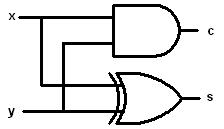
\includegraphics[scale=0.23]{Images/half-adder.png}
\todo{Improvised with PowerPoint. Redraw using Visio.}
\begin{Verbatim}
(defun and-gate (x y) (if (and (= x 1) (= y 1)) 1 0))
(defun or-gate (x y) (or (= x 1) (= y 1)))
(defun xor-gate (x y) (if (and (= x 1) (= y 1)) 0 (or-gate x y)))
(defun half-adder (x y) (list (xor-gate x y) (and-gate x y)))
\end{Verbatim}
\end{center}
\index{addition!carry}
\index{numeral!binary addition}\index{addition!binary numeral}\index{binary numeral!addition}
\index{arithmetic!binary numeral}
\index{diagram!half-adder circuit}
\index{ACL2!circuit model}\index{circuit!ACL2 model}
\index{addition!circuit}\index{circuit!addition}\index{circuit!half adder}\seeonlyindex{half adder}{circuit}
\caption{Half-Adder Circuit and ACL2 Model}
\label{fig:half-adder}
\end{figure}

Since we reason about digital circuits using the methods
of Boolean algebra, we need an algebraic representation
of the circuit-diagram for the half-adder circuit.
Remember, digital circuits are only one of four
equivalent representations of Boolean formulas that
we have studied: circuit diagrams, well-formed formulas
in the notation of mathematical logic (for example, $x \wedge y$),
Boolean formulas in engineering notation (justaposition for $\wedge$,
$+$ for $\vee$, and over-bar for $\neg$), and ACL2 notation.
The ACL2 formalization allows us mechanize some aspects of the reasoning process.
So, Figure \ref{fig:half-adder} also specifies the half-adder circuit in ACL2 terms.
We refer to this specification as an
ACL2 model of the half-adder circuit.
We use the same name for the model as the circuit:
the operator \textsf{half-adder}
delivers the two output signals as a list of two elements,
the first element being the sum bit and the second, the carry bit.

In the end, we would like to have a circuit
that adds binary numerals,
and we saw in an example (Figure \ref{fig:adding-binary-numerals})
that this would require us to deal with three input bits
in each column:
the corresponding bits in the two addends
and the carry bit brought from adding
the bits in the previous column.
The half-adder circuit is not up to this task
because it has only two input signals.
However, we can put together a full-adder circuit
by combining two half adders and a logical-or gate,
as shown in Figure \ref{fig:full-adder}
(page \pageref{fig:full-adder}).
Since the full-adder circuit has three inputs,
each of which is either 0 or 1,
there are eight possible input configurations,
as shown in the full-adder table.

\begin{figure}
\begin{center}
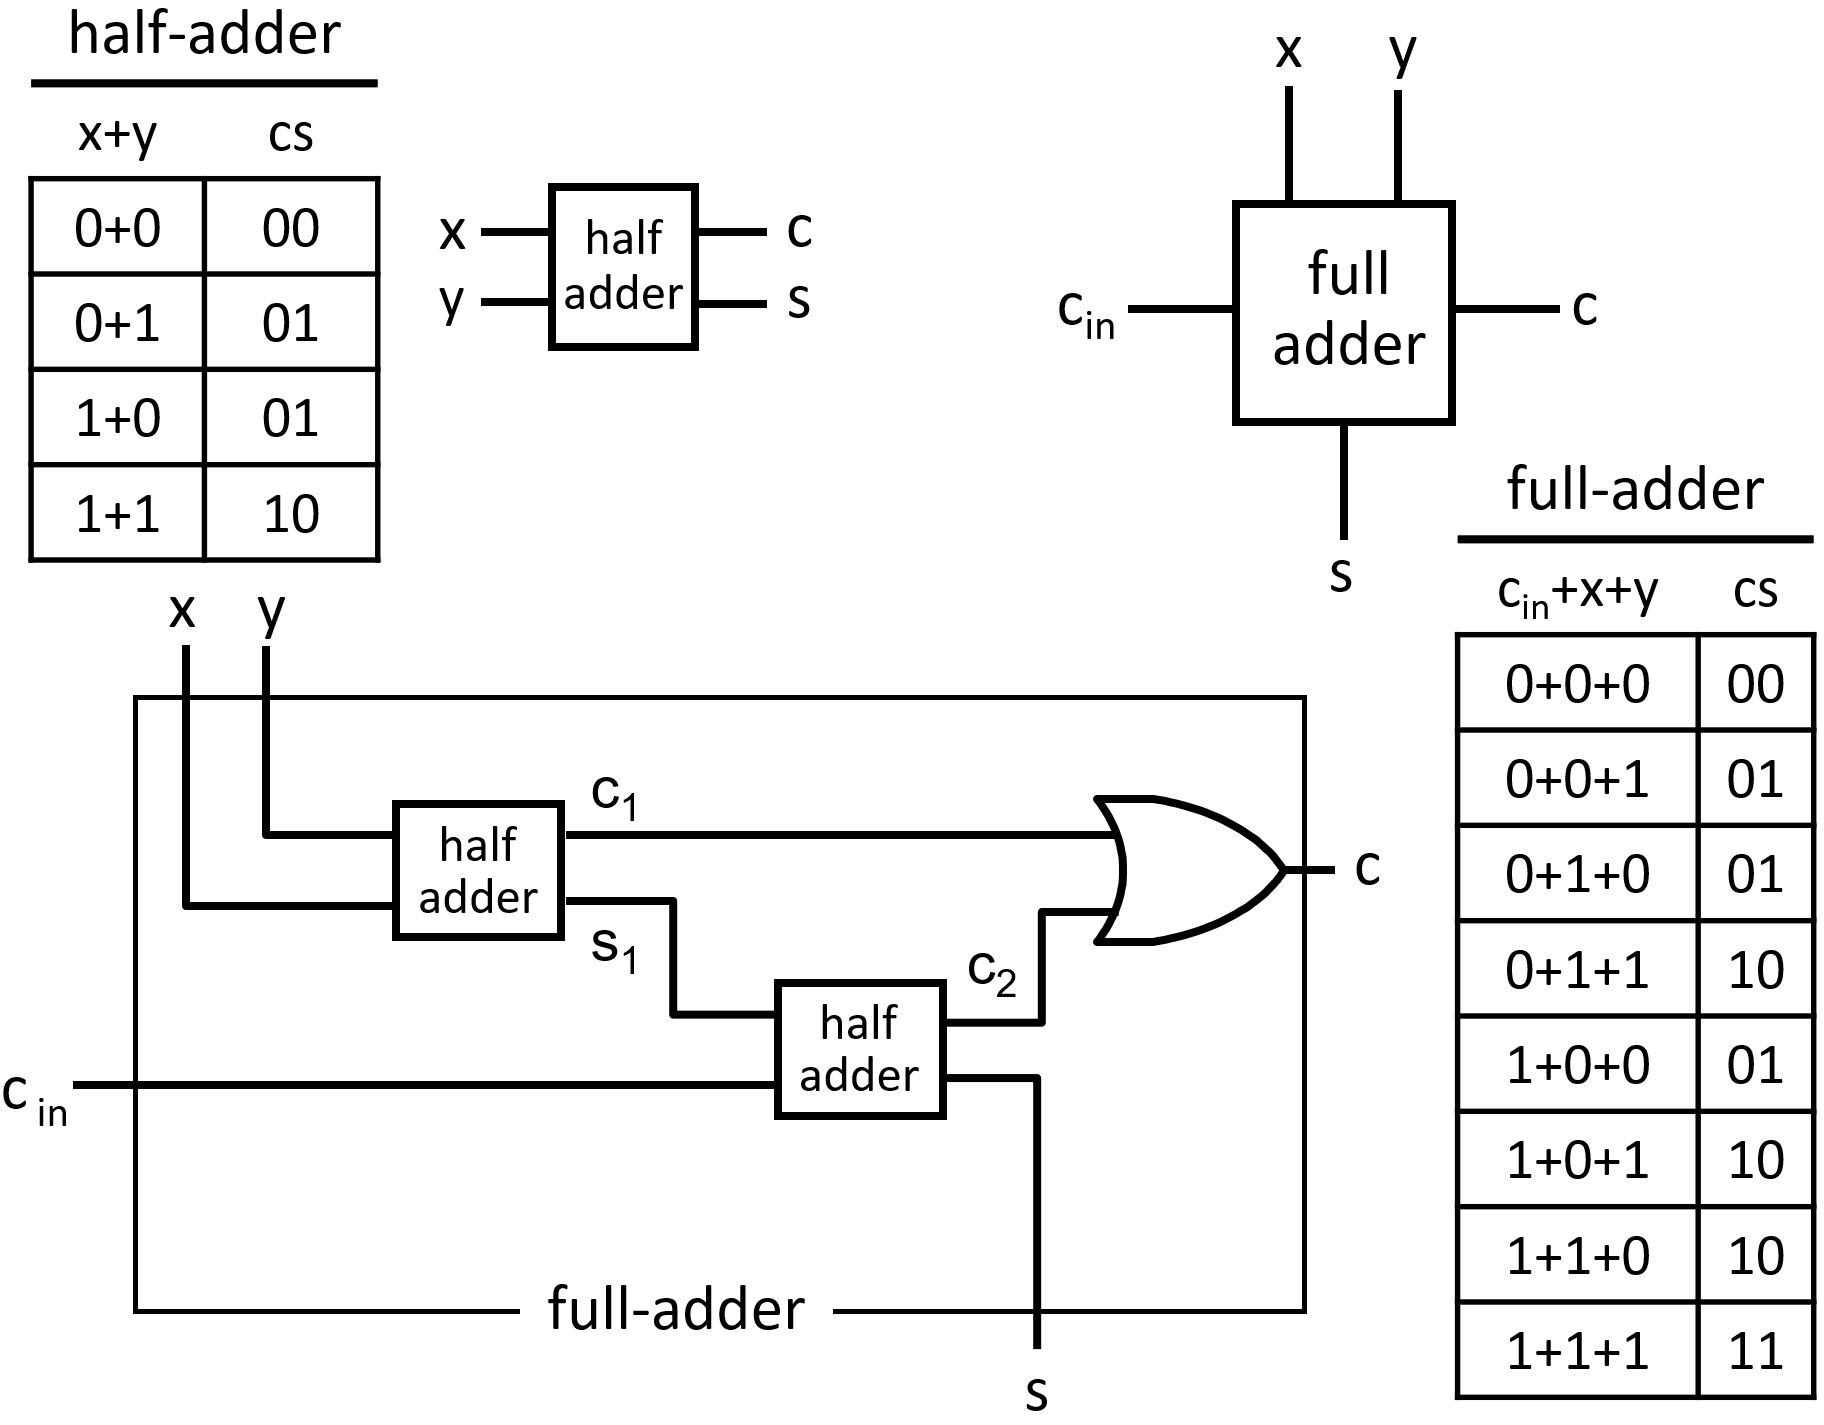
\includegraphics[scale=0.25]{Images/full-adder.png}
\todo{Improvised with PowerPoint. Redraw using Visio.}
\begin{Verbatim}
(defun full-adder (c-in x y)
  (let* ((h1 (half-adder x y))
         (s1 (first h1)) (c1 (second h1))
         (h2 (half-adder s1 c-in))
         (s  (first h2)) (c2 (second h2))
         (c  (or-gate c1 c2)))
    (list s c)))
\end{Verbatim}
\end{center}
\index{addition!carry}
\index{arithmetic!binary numeral}
\index{numeral!binary addition}\index{addition!binary numeral}\index{binary numeral!addition}
\index{diagram!full-adder circuit}
\index{addition!circuit}\index{circuit!addition}
\index{circuit!full adder}\seeonlyindex{full adder}{circuit}
\index{ACL2!circuit model}\index{circuit!ACL2 model}
\caption{Full-Adder Circuit and ACL2 Model}
\label{fig:full-adder}
\end{figure}

The \textsf{full-adder} operator defined in the figure
is a formal model in ACL2 of the circuit diagram,
and the following tests, one for each line in the table,
comprise a comprehensive, mechanized verification of
the model.

\label{full-adder-model-check}
\begin{Verbatim}
(check-expect (full-adder 0 0 0) (list 0 0))
(check-expect (full-adder 0 0 1) (list 1 0))
(check-expect (full-adder 0 1 0) (list 1 0))
(check-expect (full-adder 0 1 1) (list 0 1))
(check-expect (full-adder 1 0 0) (list 1 0))
(check-expect (full-adder 1 0 1) (list 0 1))
(check-expect (full-adder 1 1 0) (list 0 1))
(check-expect (full-adder 1 1 1) (list 1 1))
\end{Verbatim}

The \textsf{full-adder} operands
are symbols for bits, but we can use the \textsf{numb} operator
(page \pageref{nmb-defun})
to interpret them as numbers.
If $x$ is a bit, then \textsf{[$x$]} is a numeral for
the number it denotes, and the \{\emph{Horner 2}\} theorem
(Exercise \ref{horner2-thm}, page \pageref{horner2-thm})
asserts that \textsf{(numb [$x$])} computes that number.
The same theorem asserts that if $s$ and $c$ are bits,
then \textsf{(numb [$s$ $c$])} is
the number that the numeral \textsf{[$s$ $c$]} denotes.
Combining these observations with the full-adder table
(Figure \ref{fig:full-adder})
verifies the theorem \{full-adder ok\} shown in
Figure \ref{fig:full-adder-thm} (page \pageref{fig:full-adder-thm}).\footnote{The
\textsf{full-adder} operator delivers a list \textsf{[$s$ $c$]} whose first
element is the sum bit and whose second element is the carry bit.
The order of elements in the result delivered by \textsf{full-adder} was designed
to form a numeral for the sum of its three, one-bit operands.
The list in reverse order, \textsf{[$c$ $s$]},
would contain the same information,
but would not conform to our representation of binary numerals
because the low-order bit would no longer come first.}

\begin{figure}
\begin{center}
\begin{tabular}{ll}
Theorem \{\emph{full-adder ok}\} & \textsf{(numb [$s$ $c$])} $=$ \textsf{(numb [$x$])} $+$ \textsf{(numb [$y$])} $+$ \textsf{(numb [$c_{in}$])} \\
                                 & where \textsf{[$s$ $c$]} $=$ \textsf{(full-adder $c_{in}$ $x$ $y$)} \\
\end{tabular}
\begin{Verbatim}
(defthm full-adder-ok
  (= (numb (full-adder c-in x y))
     (+ (numb (list c-in)) (numb (list x)) (numb (list y)))))
\end{Verbatim}
\end{center}
\index{theorem!full adder}\seeonlyindex{full-adder theorem}{theorem}\index{theorem, by name!\{full adder-ok\}}\index{numeral!binary addition}\index{addition!binary numeral}\index{binary numeral!addition}
\caption{Full-Adder Theorem}
\label{fig:full-adder-thm}
\end{figure}

\section{Circuit for Adding Two-Bit Binary Numerals}
\label{sec:adding-2-bit-numerals}

A circuit that adds two-bit, binary numerals
comes from combining two full-adder circuits
(Figure~\ref{fig:adder2}, page \pageref{fig:adder2}).
The first full-adder circuit gets, as input, the
low-order bits, $x_0$ and $y_0$,  of the two addends.
The second full adder gets the high-order bits,
$x_1$ and $y_1$.
The circuit directs the output carry, $c_1$, from
the first full adder to the input carry of the
second full adder.

The circuit produces three output signals: one sum bit from
each full adder ($s_0$ and $s_1$) and the carry-out
from the second full adder ($c_2$).
With a carry-in of zero for the first full adder
($c_0 = 0$), the output signals form a two-bit
numeral \textsf{[$s_0$ $s_1$]} and a carry bit $c_2$
that, together, represent the sum of the two input numerals.
More generally, the output signals
represent the sum of the two input numerals and the
carry-in bit ($c_0 = 0$ or $c_0 = 1$).
The following equation \{$\star$\} shows how to interpret the
input and output signals as numbers.

\begin{center}
\textsf{(numb [$s_0$ $s_1$]) $+$ (numb [$c_2$])} $=$
\textsf{(numb [$c_0$]) $+$ (numb [$x_0$ $x_1$]) $+$ (numb [$y_0$ $y_1$])}~~~\{$\star$\}
\end{center}

\begin{figure}
\begin{center}
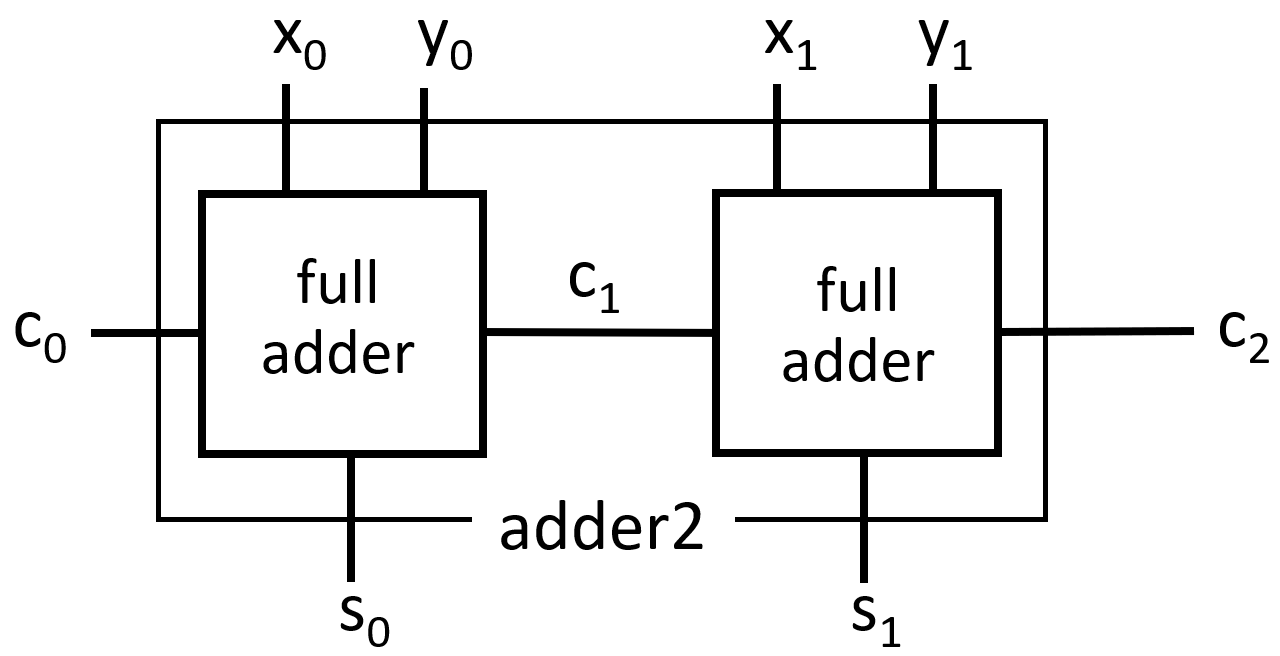
\includegraphics[scale=0.25]{Images/adder2.png}
\todo{Improvised with PowerPoint. Redraw using Visio.}
\begin{Verbatim}
(defun adder2 (c0 x y)
  (let* ((x0 (first x)) (x1 (second x))
         (y0 (first y)) (y1 (second y))
         (f0 (full-adder c0 x0 y0))
         (s0 (first f0)) (c1 (second f0))
         (f1 (full-adder c1 x1 y1))
         (s1 (first f1)) (c2 (second f1)))
    (list (list s0 s1) c2)))
\end{Verbatim}
\end{center}
\index{addition!carry}
\index{arithmetic!binary numeral}
\index{numeral!binary addition}\index{addition!binary numeral}
\index{binary numeral!addition}
\index{diagram!two-bit adder circuit}
\index{addition!circuit}\index{circuit!addition}\index{circuit!two-bit adder}\seeonlyindex{two-bit adder}{circuit}
\index{ACL2!circuit model}\index{circuit!ACL2 model}
\caption{Two-Bit Adder and ACL2 Model}
\label{fig:adder2}
\end{figure}

We refer to the output two-bit numeral, without the carry bit,
as the sum bits.
Ignoring the carry bit amounts to doing modular arithmetic, mod $2^2$
(theorem \{\emph{pfx-mod}\}, Exercise~\ref{pfx-mod}, page \pageref{pfx-mod}).

A mechanized verification of the arithmetic properties of \textsf{adder2}
could be constructed as a comprehensive sequence of \textsf{check-expect} tests,
as we did with the \textsf{full-adder} for one-bit addition
(page \pageref{full-adder-model-check}).
However, there would be 32 cases to check
because there are five bits of input
(a carry-in and two bits in each numeral, $2^5$ combinations in all).
That makes it tedious to construct a comprehensive sequence of \textsf{check-expect} tests.
It would be easy to make a mistake.

A better approach is to write equation \{$\star$\}
formally in ACL2. The equation states our expectations of
the ACL2 model of the
two-bit adder circuit (\textsf{adder2}, Figure~\ref{fig:adder2})
in the same way that the \{full-adder-ok\} theorem
(Figure \ref{fig:full-adder-thm}, page \pageref{fig:full-adder-thm})
verified the formal model of the full adder circuit.

The theorem is an equation that, on one side, is the
sum of the numeric interpretation of the input numerals
and input carry. On the other side, the equation is
the numeric interpretation of the output numeral
and output carry.
As in the \{full-adder ok\} theorem,
the \{adder2-ok\} theorem that specifies
the crucial, arithmetic property of the two-bit adder
uses the \textsf{numb} operator (page \pageref{nmb-defun})
to interpret binary numerals as numbers.

\label{adder2-ok}\index{theorem, by name!\{adder2-ok\}}\seeonlyindex{adder2 theorem}{theorem}
\begin{Verbatim}
(defthm adder2-ok
  (let* ((a (adder2 c0 (list x0 x1) (list y0 y1)))
         (s (first a)) (c (second a)))
    (= (numb (append s (list c)))
       (+ (numb (list c0))
          (numb (list x0 x1))
          (numb (list y0 y1))))))
\end{Verbatim}

\begin{ExerciseList}
\Exercise Define a DoubleCheck property that checks the
output of the two-bit adder model
(Figure \ref{fig:adder2}, page \pageref{fig:adder2})
against expectations.
Run the test using Proof Pad.\\
\emph{Note}: The data generator (random-between 0 1) delivers
a 0 or a 1 at random.

\Exercise By default, Proof Pad repeats the test fifty times
with random data
when it runs a DoubleCheck test.
How many random tests do you think would be needed to be reasonably
confident that all 32 different cases for the two-bit adder have been tested?
\end{ExerciseList}

\section{Adding w-Bit Binary Numerals}
\label{sec:adding-w-bit-numerals}

By now, you can predict what a circuit for adding three-bit
binary numerals would look like.
Put another full adder in the circuit, and feed the
high-order bits from the two numerals into the new full adder.
In addition, connect the carry-out from the two-bit circuit
to the carry-in, of the new full adder.
A two-bit adder circuit augmented in this way
becomes a circuit for adding three-bit numerals.
A circuit diagram for adding numerals with any number of bits
combines the appropriate number of
full-adder components in this manner.
Figure \ref{fig:adder} (page \pageref{fig:adder}) presents a schematic
for a circuit that adds \emph{w}-bit numerals.
The circuit is known as a \emph{ripple-carry adder} because
of the way the carry-bit propagates across the line
of full-adder components.

\begin{figure}
\begin{center}
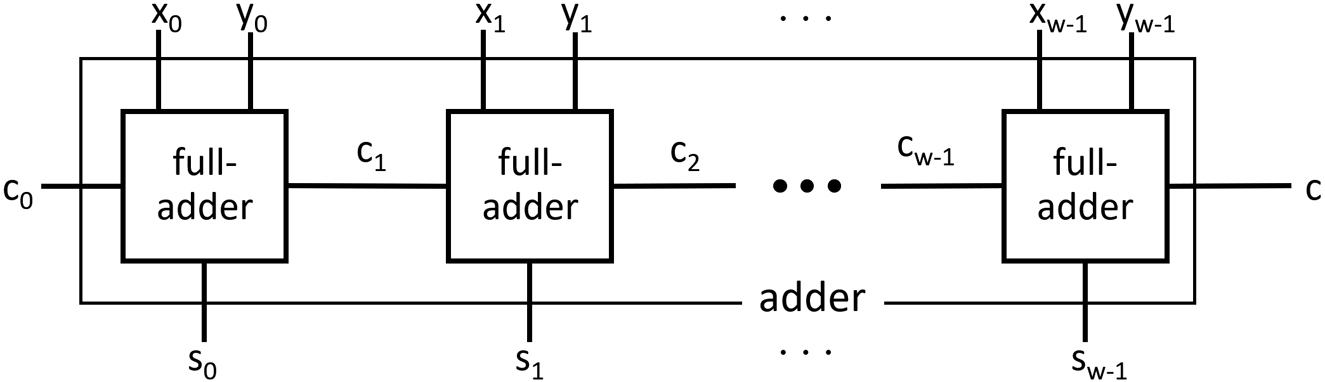
\includegraphics[scale=0.25]{Images/adder.png}
\todo{Improvised with PowerPoint. Redraw using Visio.}
\begin{Verbatim}
(defun adder (c0 x y)
  (if (consp x)
      (let* ((x0 (first x)) (xs (rest x))
             (y0 (first y)) (ys (rest y))
             (a0 (full-adder c0 x0 y0))
             (s0 (first a0)) (c1 (second a0)) ; {add.bit0}
             (a  (adder c1 xs ys))
             (ss (first a)) (c (second a)))   ; {add.bits}
        (list (cons s0 ss) c))                ; {add1}
      (list nil c0)))                         ; {add0}
\end{Verbatim}
\end{center}
\index{equation, by name!\{addo\}, \{add1\}}\index{addition!carry}\index{arithmetic!binary numeral}\index{numeral!binary addition}\index{addition!binary numeral}\index{binary numeral!addition}\index{diagram!ripple-carry circuit}\index{addition!circuit}\index{circuit!addition}\index{circuit!ripple-carry adder}\seeonlyindex{ripple-carry circuit}{circuit}\index{ACL2!circuit model}\index{circuit!ACL2 model}
\caption{Ripple-Carry Adder and ACL2 Model}
\label{fig:adder}
\end{figure}

The ACL2 model in the figure relies
on inductive definition. It feeds the carry-in and
the low-order bits from the two numerals into the \textsf{full-adder} operator.
(The low-order bit in a numeral is the ``ones bit,''
which is the first element of the list that we use to
represent the numeral.)
The sum bit from the list that the \textsf{full-adder} operator delivers
is the low-order bit of the numeral representing the sum of
the numbers that the input numerals represent.
The remaining sum bits in the list are those delivered by
the \textsf{adder} operating on the other bits in the input numerals
(that is, all the bits in the input numerals except the low-order bits).

Because the model defines an operator in ACL2,
you can run the operator to see that it works in specific cases.
To add two binary numerals, supply lists of
\index{zeros \& ones}\index{ones \& zeros}
0s and 1s
representing those numerals in an invocation
of the \textsf{adder} operator, and specify zero as the input carry-bit.
The output will be binary numeral for the sum.

The theorem in Figure \ref{fig:adder-thm} (page \pageref{fig:adder-thm})
explains how input and output signals are interpreted as numbers.
As with the two-bit adder (Figure \ref{adder2-ok}, page \pageref{adder2-ok})
the three numbers represented by the two input
numerals and the input carry, when added together,
equal the number represented
by a numeral formed from the output sum-bits and
the output carry-bit.
However, the theorem for the \emph{w}-bit adder
is stated as an implication to constrain
inputs to be numerals with the same number of bits.
This was not necessary with the theorem for the two-bit adder
because the lengths of the numerals were explicit in the ACL2 model.

\begin{figure}
\begin{center}
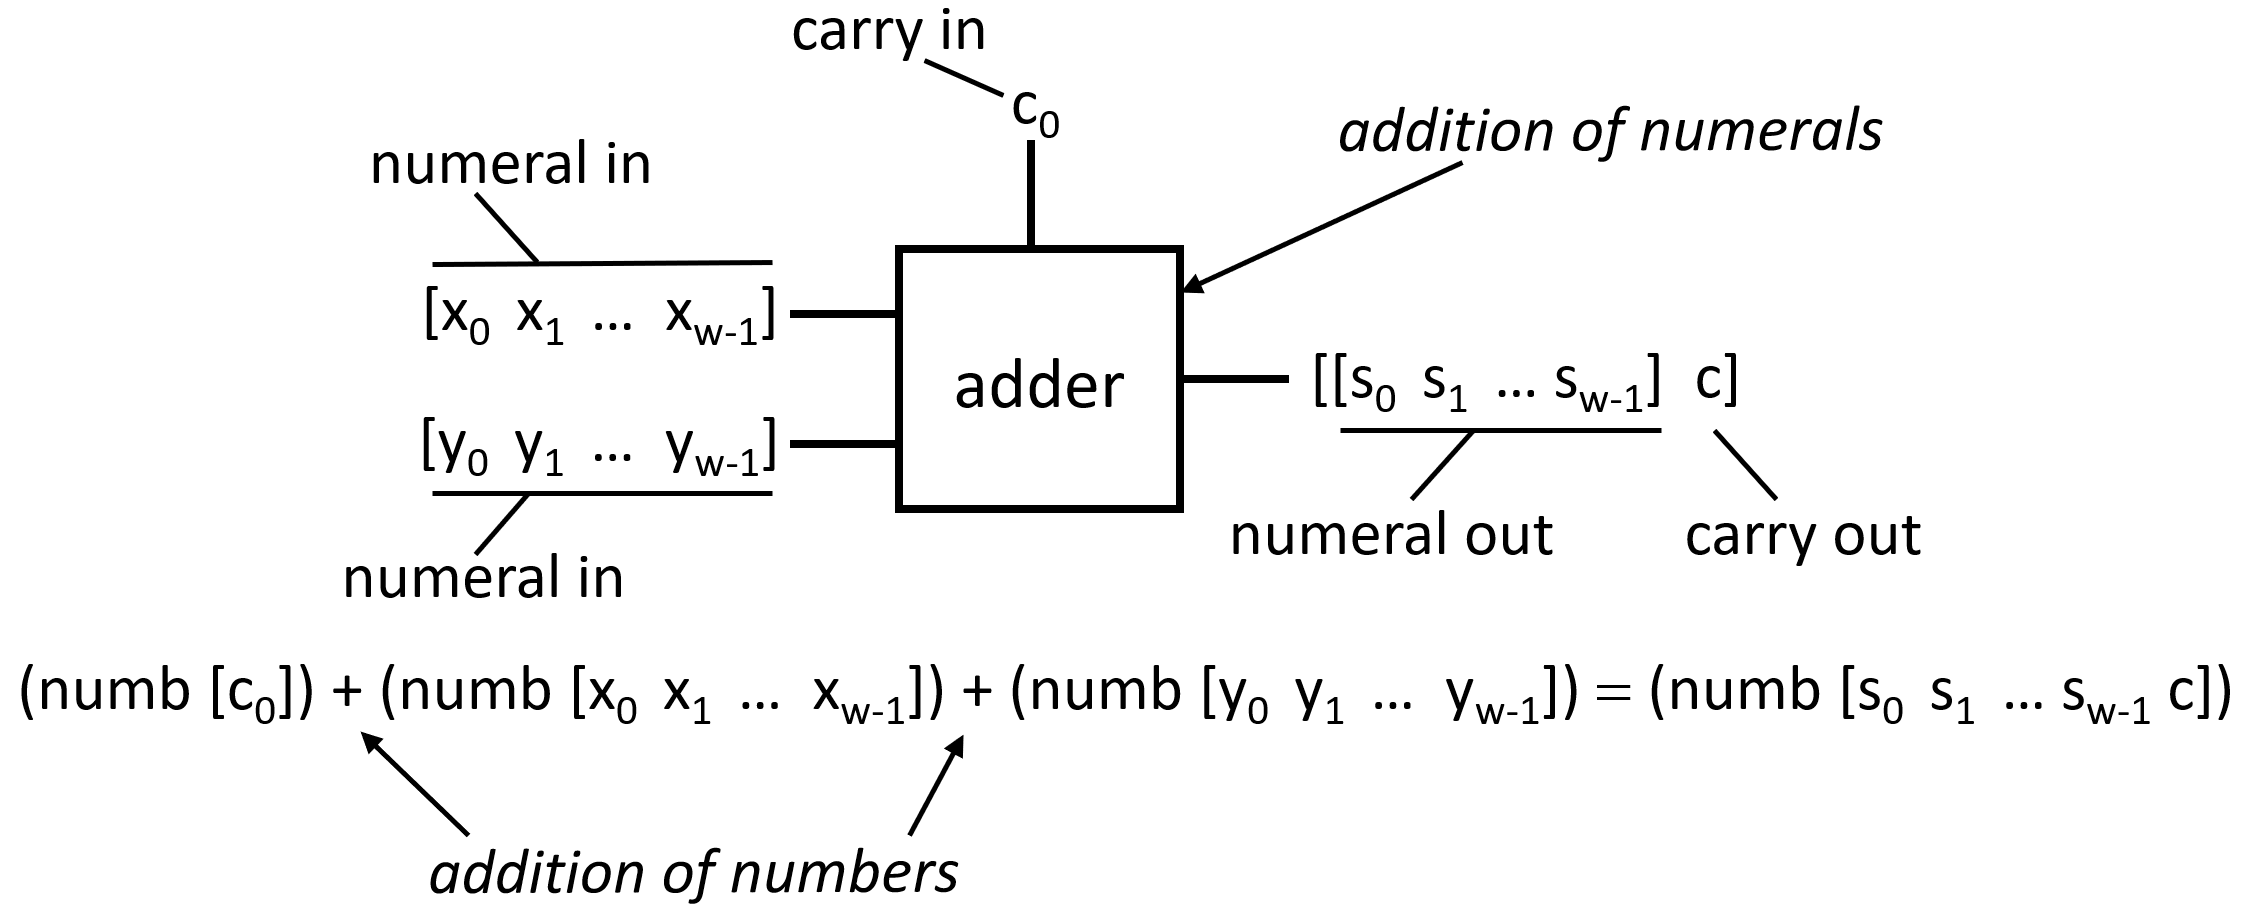
\includegraphics[scale=0.3]{Images/adder-thm.png}
\todo{Improvised with PowerPoint. Redraw using Visio.}
\begin{Verbatim}
(defthm adder-ok
  (implies (= (len x) (len y))
           (let* ((a (adder c0 x y))
                  (s (first a)) (c (second a)))
             (= (numb (append s (list c)))
                (+ (numb (list c0)) (numb x) (numb y))))))
\end{Verbatim}
\end{center}
\seeonlyindex{ripple-carry theorem}{theorem}\index{theorem, by name!\{adder-ok\}}\index{theorem!ripple-carry adder}\index{ACL2!adder-ok}\index{arithmetic!binary numeral}\index{numeral!binary addition}\index{addition!binary numeral}\index{binary numeral!addition}
\caption{Adding \emph{w}-Bit Binary Numerals}
\label{fig:adder-thm}
\end{figure}

Theorem \{adder-ok\} (Figure~\ref{fig:adder-thm}, page \pageref{fig:adder-thm})
states the arithmetic property that we expect the adder circuit to have.
The mechanized logic of ACL2 succeeds in verifying
the theorem without assistance,
but because reasoning about circuits is such an important idea,
we think going through
a paper-and-pencil proof will be worthwhile.
Our proof will, of course, work from
the model of the adder circuit
(Figure \ref{fig:adder}, page \pageref{fig:adder}),
rather than from the circuit diagram.
Aside \ref{circuit-vs-model} (page \pageref{circuit-vs-model})
discusses some of the ramifications of this approach,
which has been our basis for reasoning about circuits.

\begin{aside}
We expect that you could, given a basket of
logic gates, wires, and enough time,
use the diagram of the adder circuit to
build one for any specified word size,
and we think you can convince yourself that the model
matches the diagram.
If it does, then properties of the model
that we verify guarantee that the circuits also have those properties.

In a complete formalization, we would
need a way to convert models into instructions
for fabricating circuits so that
the fabricated circuit would have the properties
of the model. Such a formalization
would use the methods we have employed to formalize other operations.
We leave that step to the imagination.
\index{circuit!ACL2 model}\index{model!of circuit}
\caption{Models and Circuit Fabrication}
\label{circuit-vs-model}
\end{aside}
%\begin{samepage}
%\label{adder-thm}\index{theorem, by name!\{adder-ok\}}\index{theorem!ripple-carry adder}\seeonlyindex{ripple-carry theorem}{theorem}\index{numeral!binary addition}\index{addition!binary numeral}\index{binary numeral!addition}
%\begin{center}
%\begin{tabular}{l}
%Theorem \{\emph{adder ok}\} \\
%\textsf{(numb [$s_0$ $s_1$ \dots $s_{n}$ $c$])} $=$
%\textsf{(numb [$c_0$])} $+$ \textsf{(numb [$x_0$ $x_1$ \dots $x_{n}$])} $+$ \textsf{(numb [$y_0$ $y_1$ \dots $y_{n}$])} \\
%where \textsf{[[$s_0$ $s_1$ \dots $s_{n}$] $c$]} $=$ \textsf{(adder $c_0$ [$x_0$ $x_1$ \dots $x_{n}$] [$y_0$ $y_1$ \dots $y_{n}$])}\\
%\end{tabular}
%\end{center}
%\end{samepage}

Figure \ref{fig:adder-thm-prf} (page \pageref{fig:adder-thm-prf})
displays the \{adder ok\} theorem in algebraic notation.
Proving the theorem amounts to
verifying that $(\forall n.R(n))$ is true,
where the predicate $R$, which has the natural numbers as
its universe of discourse, is defined as follows.
\begin{center}
\begin{tabular}{l}
$R(n) \equiv$ $($\textsf{(numb [$s_0$ $s_1$ \dots $s_{n}$ $c$])} $=$\\
\phantom{$R(n) \equiv$ $($}\textsf{(numb [$c_0$])} $+$ \textsf{(numb [$x_0$ $x_1$ \dots $x_{n}$])} $+$ \textsf{(numb [$y_0$ $y_1$ \dots $y_{n}$])}$)$ \\
~~~~~ where \textsf{[[$s_0$ $s_1$ \dots $s_{n}$] $c$]} $=$ \textsf{(adder $c_0$ [$x_0$ $x_1$ \dots $x_{n}$] [$y_0$ $y_1$ \dots $y_{n}$])}\\
\end{tabular}
\end{center}

The proof will use mathematical induction.
Figure~\ref{fig:adder-thm-prf}
displays the equation of the base case, $R(0)$,
and sketches its proof. Here we elaborate some of the details
that were omitted in the sketch.
The first step is
to compute the value of \textsf{(adder $c_0$ [$x_0$] [$y_0$])}
by working through the definition of the \textsf{adder} operator
(Figure \ref{fig:adder}, page \pageref{fig:adder}).
With those operands, the \textsf{if} operator in
the definition of \textsf{adder} selects the \{add1\} equation.
\begin{quote}
\begin{tabular}{rll}
       & \textsf{(adder $c_0$ [$x_0$] [$y_0$])}              & \\
\vspace{1mm}
$=$    & \textsf{[(cons $s_0$ $ss$) $c$]}                    & \{add1\} (page \pageref {fig:adder})  \\
where  &&\\
       & \textsf{[$ss$  $c$]}                                & \\
$=$    & \textsf{(adder $c_1$ (rest [$x_0$]) (rest [$y_0$]))}& \{add.bits\} (page \pageref {fig:adder}) \\
$=$    & \textsf{(adder $c_1$ nil nil)}                      & \{\emph{rst1}\} (page \pageref {rst1}) \\
$=$    & \textsf{[nil  $c_1$]}                               & \{add0\} (page \pageref {fig:adder}) \\
\end{tabular}
\end{quote}
\addtolength{\tabcolsep}{-1mm}
\begin{tabular}{rll}
Therefore, & $ss$ $=$ \textsf{nil}                                       & \\
           & $c$ $=$ $c_1$                                      & \{$\dagger$\} \\
and        & \textsf{(cons $s_0$ $ss$}) $=$ \textsf{(cons $s_0$ nil)} $=$ \textsf{[$s_0$]} & \{$\ddagger$\}\\
           &                                                    & \\
\end{tabular}\\
\addtolength{\tabcolsep}{1mm}
The equation $R(0)$ (Figure~\ref{fig:adder-thm-prf}) makes the following requirement.
\vspace{1mm}\\
\hspace*{1.5cm}\textsf{[[$s_0$] $c$]} $=$ \textsf{(adder $c_0$ [$x_0$] [$y_0$])}
~~\vspace{2mm}\\
The following argument, which proceeds
from the right-hand side to the left-hand side of the requirement,
confirms that it is consistent with the definition of the \textsf{adder} operator.\\
\begin{tabular}{rll}
 ~~~~~~~~& \textsf{(adder $c_0$ [$x_0$] [$y_0$])} & \\
$=$ & \textsf{[(cons $s_0$ $ss$) $c$]}       & \{add1\}      \\
$=$ & \textsf{[[$s_0$] $c$]}                 & \{$\ddagger$\}\\
\end{tabular}
~~\vspace{2mm}\\
The proof of the base case can be completed as follows.\\
\begin{tabular}{rll}
 ~~~~~~~~& \textsf{(numb [$s_0$ $c$])}                               &                   \\
$=$ & (\textsf{numb [$s_0$ $c_1$])}                             & \{$\dagger$\}    \\
$=$ & \textsf{(numb (full-adder $c_0$ $x_0$ $y_0$))}            & \{add.bit0\}      \\
$=$ & \textsf{(numb [$c_0$])} + \textsf{(numb [$x_0$])} $+$ \textsf{(numb [$y_0$])} & \{full-adder-ok\} \\
\end{tabular}\\

So much for the base case.
Figure~\ref{fig:adder-thm-prf} also presents
a proof of the inductive case: $\forall n.(R(n) \rightarrow R(n+1))$.
When that proof arrives at the sum
\textsf{(numb [$c_1$])} $+$ \textsf{(numb [$x_1$ \dots $x_{n+1}$])} $+$ \textsf{(numb [$y_1$ \dots $y_{n+1}$])},
it recognizes that the induction hypothesis, $R(n)$, applies because
the numerals \textsf{[$x_1$ \dots $x_{n+1}$]} and \textsf{[$y_1$ \dots $y_{n+1}$]} have $n+1$
elements, like the numerals in the equation $R(n)$.
The subscripts run from $1$ to $n+1$ instead of from $0$ to $n$,
but it's the number of bits that counts, not the subscripts.

The induction hypothesis says that this sum equals
\textsf{(numb [$s_1$ \dots $s_{n+1}$ $c$])}, and
the \{\emph{nmb1}\} theorem (Exercise \ref{nmb1}, page \pageref{nmb1})
adds \textsf{(numb [$s_0$])} $+$ $2\times$\textsf{(numb [$s_1$ \dots $s_{n+1}$ $c$])}
to arrive at \textsf{(numb [$s_0$ $s_1$ \dots $s_{n}$ $c$])}.
We have derived the left-hand side
of equation $R(n+1)$, having started from the right-hand side.
That completes the proof of the \{adder ok\} theorem
by mathematical induction.

The proof is tedious, to say the least.
It requires working out the details of
numerous operator invocations
from symbolic representations of the operands.
Fortunately, ACL2 is on hand to work through the
muck and mire and arrive at the same conclusion.
That gives us confidence that our ripple-carry circuit
for adding binary numerals delivers the expected results.

\begin{figure}
Theorem \{adder ok\}\\
$\forall n.($\textsf{(numb [$s_0$ $s_1$ \dots $s_{n}$ $c$])} $=$
\textsf{(numb [$c_0$])} $+$ \textsf{(numb [$x_0$ $x_1$ \dots $x_{n}$])} $+$ \textsf{(numb [$y_0$ $y_1$ \dots $y_{n}$])}$)$\\
\hphantom{(numb}where \textsf{[[$s_0$ $s_1$ \dots $s_{n}$] $c$]} $=$ \textsf{(adder $c_0$ [$x_0$ $x_1$ \dots $x_{n+1}$] [$y_0$ $y_1$ \dots $y_{n}$])}\\
\emph{Base Case}
\begin{center}
\begin{tabular}{l}
\hline
$R(0) \equiv$  $($\textsf{(numb [$s_0$ $c$])} $=$ \textsf{(numb [$c_0$])} $+$ \textsf{(numb [$x_0$])} $+$ \textsf{(numb [$y_0$])}$)$ \\
 ~~~~~~ where \textsf{[[$s_0$] $c$]} $=$ \textsf{(adder $c_0$ [$x_0$] [$y_0$])} \\
\hline
\end{tabular}
\begin{tabular}{ll}
\textsf{(adder $c_0$ [$x_0$] [$y_0$])} $=$ \textsf{[(cons $s_0$ nil) $c$]} $=$ \textsf{[[$s_0$] $c$]} & \{\emph{add1}\} (\{\emph{adder}\} \emph{Fig. \ref{fig:adder}, p.\pageref{fig:adder}}) \\
~~~~ where \textsf{[$s_0$ $c$]} $=$ \textsf{(full-adder $c_0$ $x_0$ $y_0$)}          & \emph{note:} (adder $c$ nil nil) = [nil $c$] \\
\textsf{(numb [$s_0$ $c$])} = \textsf{(numb (full-adder $c_0$ $x_0$ $y_0$)}          &  \\
~~~~~~~~~~~ $=$ \textsf{(numb [$c_0$])} $+$ \textsf{(numb [$x_0$])} $+$ \textsf{(numb [$y_0$])}  & \{\emph{full-adder ok}\} \emph{(Fig. \ref{fig:full-adder-thm}, p.\pageref{fig:full-adder-thm})}\\
\end{tabular}
\end{center}
\emph{Inductive Case}
\begin{center}
\begin{tabular}{l}
 \hline
$R(n+1)$ $\equiv$ $($\textsf{(numb [$s_0$ $s_1$ \dots $s_{n+1}$ $c$])} $=$ \\
\hphantom{$R(n+1)$ $\equiv$ $($}\textsf{(numb [$c_0$])} $+$ \textsf{(numb [$x_0$ $x_1$ \dots $x_{n+1}$])} $+$ \textsf{(numb [$y_0$ $y_1$ \dots $y_{n+1}$])}$)$ \\
 ~~~~~~ where \textsf{[[$s_0$ $s_1$ \dots $s_{n+1}$] $c$]} $=$ \textsf{(adder $c_0$ [$x_0$ $x_1$ \dots $x_{n+1}$] [$y_0$ $y_1$ \dots $y_{n+1}$])} \\
\hline
\end{tabular}
\begin{tabular}{ll}
\hspace*{3mm}\textsf{(numb [$c_0$])} $+$ \textsf{(numb [$x_0$ $x_1$ \dots $x_{n+1}$])} $+$ \textsf{(numb [$y_0$ $y_1$ \dots $y_{n+1}$])}& \\
$=$ \textsf{(numb [$c_0$])} $+$ \textsf{(numb [$x_0$])} $+$ $2\times$\textsf{(numb [$x_1$ \dots $x_{n+1}$])}                         & \{\emph{nmb1}\} \emph{(p. \pageref{nmb1})} \\
\hphantom{$=$ \textsf{(numb [$c_0$])} }$+$ \textsf{(numb [$y_0$])} $+$ $2\times$\textsf{(numb [$y_1$ \dots $y_{n+1}$])}                  & \{\emph{nmb1}\} \\
$=$ \textsf{(numb [$c_0$])} $+$ \textsf{(numb [$x_0$])} $+$ \textsf{(numb [$y_0$])} $+$                                                & \\
 ~~~~~~ $2\times($\textsf{(numb [$x_1$ \dots $x_{n+1}$])} $+$ \textsf{(numb [$y_1$ \dots $y_{n+1}$])}$)$                    & \{\emph{algebra}\} \\
$=$ \textsf{(numb (full-adder $c_0$ $x_0$ $y_0$))} $+$                                                             & \{\emph{full-adder ok}\} \\
 ~~~~~~ $2\times($\textsf{(numb [$x_1$ \dots $x_{n+1}$])} $+$ \textsf{(numb [$y_1$ \dots $y_{n+1}$])}$)$                    & \\
$=$ \textsf{(numb [$s_0$ $c_1$])} $+$ $2\times($\textsf{(numb [$x_1$ \dots $x_{n+1}$])} $+$ \textsf{(numb [$y_1$ \dots $y_{n+1}$])}$)$ & \{\emph{add.bit0}\} \emph{(p.\pageref{fig:full-adder-thm})} \\
$=$ \textsf{(numb [$s_0$])} $+$ $2\times$\textsf{(numb [$c_1$])} $+$                                                          & \{\emph{nmb1}\} \\
\hphantom{$=$ \textsf{(numb [$s_0$])} $+$ }$2\times($\textsf{(numb [$x_1$ \dots $x_{n+1}$])} $+$ \textsf{(numb [$y_1$ \dots $y_{n+1}$])}$)$  & \\
$=$ \textsf{(numb [$s_0$])} $+$                                                                                    & \{\emph{algebra}\} \\
 ~~~~~~ $2\times($\textsf{(numb [$c_1$])} $+$ \textsf{(numb [$x_1$ \dots $x_{n+1}$])} $+$ \textsf{(numb [$y_1$ \dots $y_{n+1}$])}$)$ & \\
$=$ \textsf{(numb [$s_0$])} $+$ $2\times$\textsf{(numb [$s_1$ \dots $s_{n+1}$ $c$])}                                        & \{$R(n)$\} \\
$=$ \textsf{(numb [$s_0$ $s_1$ \dots $s_{n+1}$ $c$])}                                                              & \{\emph{nmb1}\} \\
\end{tabular}
\end{center}
\index{theorem, by name!\{adder-ok\}}\seeonlyindex{adder-ok theorem}{theorem}\index{theorem!ripple-carry adder}\index{numeral!binary addition}\index{addition!binary numeral}\index{binary numeral!addition}\index{arithmetic!binary numeral}
\caption{Theorem \{adder ok\}: Proof by Mathematical Induction}
\label{fig:adder-thm-prf}
\end{figure}

\begin{aside}
A \emph{word} in a computer is a collection of bits
that the computer treats as a whole in certain operations,
such as arithmetic operations.
A circuit to perform arithmetic will carry out
the operation on words denoting binary numerals.
Since all words have the same number of bits,
both of the numerals supplied as inputs to circuit
for an arithmetic operator will have the same number of bits.

We could change the design of the circuit for the adder
to accommodate input numerals of differing lengths.
However, since we are modeling a circuit
in which the input numerals have the same length,
the model does not need to account for that possibility.
\index{word!computer}\index{computer word}
\caption{Adder Circuit and Numerals of Different Lengths}
\label{adder-circuit-and-numerals-of-different-lengths}
\end{aside}

\begin{ExerciseList}
\Exercise \label{ex:add-bin}
Define in ACL2 a operator \textsf{add-bin}
that adds any two binary numerals,
even if the numerals contain a different number of bits.
That is, the value \textsf{(add-bin $c$ $x$ $y$)} should be a binary numeral
for the number \textsf{(numb [$c$])} $+$ \textsf{(numb $x$)} $+$ \textsf{(numb $y$)},
as long as $x$ and $y$ are binary numerals and $c$ is 0 or 1,
regardless of \textsf{(len $x$)} or \textsf{(len $y$)}.
Design and run some sanity checks on your operator.

\Exercise Define in ACL2 a theorem about the operator \textsf{add-bin} (Excercise \ref{ex:add-bin})
that is analogous to theorem \{adder-ok\}
(Figure \ref{fig:adder-thm}, page \pageref{fig:adder-thm}).

\end{ExerciseList}

\section{Numerals for Negative Numbers}
\label{sec:negative-numerals}

So far, all the numerals we've seen have denoted positive numbers.
Arithmetic circuits also need to deal with negative numbers,
and there is more than one way to do that.
The most common scheme is known as the \emph{twos complement} system.

\index{negative numeral}\index{numeral!negative}\index{number!negative}\index{numeral!twos complement}\index{twos complement!numeral}Twos-complement
numerals are a special interpretation of
ordinary binary numerals.
For the numbers $0$, $1$, $\dots$ $(2^{w-1}-1)$,
where \emph{w} is the \emph{word size}
of the circuits for arithmetic operations,
twos-complement numerals are ordinary binary numerals.
All of the numerals for this set of numbers
have $(w-1)$ or fewer bits,
not counting leading zeros
(Theorem \{\emph{len-bits}$\le$\}, page \pageref{len-bitsLE}).
To make the numerals match the word size,
the twos-complement system pads them with leading zeros
to make them have exactly \emph{w} bits.
Leading zeros don't change the number that a numeral denotes
(Theorem \{\emph{leading-0s}\}, page \pageref{leading-0s}), but,
as with the ripple-carry adder (Figure \ref{fig:adder}, page \pageref{fig:adder}),
circuits to perform arithmetic on twos-complement numbers will
require exactly \emph{w} bits for each input numeral
because there are $w$ input lines for each addend,
and each input line must carry a signal.
The non-negative numbers, $0$, $1$, \dots $(2^{w-1}-1)$
consume half of the $2^w$ bit-patterns available with
\emph{w}-bit words.

For negative numbers,
the twos-complement system uses the other half of the bit-patterns.
These are the numerals that would normally denote the numbers
$2^{w-1}$, $(2^{w-1}+1)$, \dots $(2^{w}-1)$.
If $(-n)$ is a negative number in the range $-2^{w-1} \leq (-n) < 0$,
\label{2s-def}
then the twos-complement numeral for $(-n)$
is the ordinary binary numeral for $(2^w - n)$.
Since $2^{w-1} = (2^{w}-2^{w-1}) \leq (2^w - n) < 2^w$,
this numeral has exactly \emph{w} bits
(Theorem \{\emph{len-bits}\}, page \pageref{len-bits}).
We also know that its high-order bit is a one-bit
(Theorem \{\emph{hi-1}\}, page \pageref{hi-1}),
so there is an easy way to recognize numerals that denote negative numbers.

For example, a computer with
\index{twos complement!word}\index{word!twos complement}
\index{word!computer}\index{computer word}32-bit words that uses
two-complement numerals has arithmetic circuits that
deal with numbers $n$ in the range $-2^{w-1} \leq n < 2^{w-1}$.
In the positive part of the range, it represents numbers as
ordinary binary numerals, but with enough leading zeros
to fill the 32-bit word.
For a number ($-n$) in the negative part of the range,
the twos-complement system uses the ordinary binary numeral
for the positive number ($2^{32}-n$) to represent the number ($-n$).
Since ($-n$) is in the range
$-2^{31} \leq -n < 0$, we can assert that
$2^{31} = 2^{32}-2^{31} \leq 2^{32}-n < 2^{32}$.
Therefore, the twos-complement, binary numeral
for the negative number ($-n$)
has exactly 32 bits (Theorem \{\emph{len-bits}\}, page \pageref{len-bits}).

\index{negative numeral}\index{numeral!negative}\index{number!negative}
\index{numeral!twos complement}\index{twos complement!numeral}
Modular arithmetic makes twos-complement numerals
for negative numbers act like the negative numbers they stand for
when they are added to other numerals.
For negative numbers ($-n$) in the range $-2^{31} \leq -n < 0$,
the value of (($-n$) mod $2^{32}$) is ($2^{32}-n$).
Therefore, since addition and subtraction
in modular arithmetic is consistent with ordinary addition and subtraction
(Aside~\ref{modular-arithmetic}, page \pageref{modular-arithmetic}), it follows that
  ($(m+(-n))$ mod $2^{32}$
= (($m$ mod $2^{32}$) $+$ ($(-n)$ mod $2^{32}$)) mod $2^{32}$
= $((m$ mod $2^{32}$) $+$ $((2^{32} - n)$ mod $2^{32}))$ mod $2^{32}$.

That is, adding the numbers represented by twos-complement
numerals, including numbers in the negative range,
is just like adding ordinary numbers in modular arithmetic.
Subtraction is handled by negating a number
(that is, computing the twos-complement representation
of its negative), then performing addition modulo $2^{32}$.

This method works for any word size.
With word size $w$, the twos complement system
handles addition and subtraction for numbers $n$
in the range $-2^{w-1} \leq n < 2^{w-1}$
by performing ordinary addition of numerals,
as with the ripple-carry adder, but interpreting
the numerals according to the twos-complement scheme.
Circuits for performing addition (and subtraction, which
uses the same circuit in a twos-complement system)
take advantage of the consistency between modular arithmetic
and ordinary arithmetic.

In summary, the twos-complement representation for computers with
word size $w$ deals with numbers $n$ in the range
$-2^{w-1} \leq n < 2^{w-1}$.
We will refer to this set of integers as $I(w)$.
\label{def-Iw}
\begin{center}
$I(w) = \{-2^{w-1}, \dots -1, 0, 1, 2, \dots 2^{w-1}-1\}$
\end{center}

\index{negative numeral}\index{numeral!negative}\index{number!negative}
\index{numeral!twos complement}\index{twos complement!numeral}
\index{twos complement!word}
Twos-complement numerals for numbers in the negative part of the range
have exactly $w$ bits, with a one-bit in the high-order slot.
Twos-complement numerals for numbers in the positive part of $I(w)$
take the form of ordinary binary numerals, except that
they are padded with enough leading zeros
to fill out a $w$-bit word, where $w$ is the word size of the computer.
The \textsf{twos} operator, defined as follows, delivers the twos-complement numeral
for a number $n$ in the set $I(w)$.

\label{twos-defun}\index{twos complement!operator}\index{operator, by name!twos (twos complment)}\index{operator!twos complement}\index{equation, by name!\{2s$+$\}, \{2s$-$\}}\index{arithmetic!negative numeral}
\begin{Verbatim}
(defun twos (w n)             ; w = word size
  (if (< n 0)                 ; -2^(w-1) <= n < 2^(w-1)
      (bits (+ (expt 2 w) n)) ; {2s-}
      (pad w 0 (bits n))))    ; {2s+}
\end{Verbatim}

The \textsf{twos} operator uses the operator \textsf{bits} (page \pageref{bits-defun})
to compute binary numerals.
For negative numbers it adds $2^w$
(that is, \textsf{(expt $2$ $w$)}, 
using the ACL2 intrinsic operator \textsf{expt})
before computing the numeral.
For non-negative numbers, it computes the numeral,
then uses the \textsf{pad} operator (Exercise~\ref{ex:pad-defun}, page \pageref{ex:pad-defun})
to insert leading zeros to match the word-size.
There will always be some padding for numerals representing
positive numbers because
$0 \le n < 2^{w-1}$ implies that
$0 \le $(len (bits $n$)) $< w$
(Theorem \{\emph{len-bits}$\le$\}, page \pageref{len-bitsLE}).

Figure~\ref{fig:2s-comp-3bit} displays
twos-complement numerals for the numbers in the set $I(3)$.
This example is just to illustrate the idea.
No computer would have three-bit words,
but the example gets the point across with a table of manageable size.

\begin{figure}
\begin{center}
\begin{tabular}{cccc}
 $n \in I(3)$ & $2^3+n$  & \textsf{(twos $3$ $n$)}   & \emph{binary numeral} \\
 $-4$         & $4$      & \textsf{[0 0 1]}          & 100                   \\
 $-3$         & $5$      & \textsf{[1 0 1]}          & 101                   \\
 $-2$         & $6$      & \textsf{[0 1 1]}          & 110                   \\
 $-1$         & $7$      & \textsf{[1 1 1]}          & 111                   \\
 $~~0$        &          & \textsf{[0 0 0]}          & 000                   \\
 $~~1$        &          & \textsf{[1 0 0]}          & 001                   \\
 $~~2$        &          & \textsf{[0 1 0]}          & 010                   \\
 $~~3$        &          & \textsf{[1 1 0]}          & 011                   \\
\end{tabular}
\\ $I(w) = I(3) = \{-2^{3-1}=-4, -3, -2, -1, 0, 1, 2, 3=2^{3-1}-1\}$
\\ \emph{word size} $w = 3$
\end{center}
\index{negative numeral}\index{numeral!negative}\index{number!negative}\index{numeral!twos complement}\index{twos complement!numeral}\index{twos complement!word}\index{word!twos complement}\index{arithmetic!negative numeral}
\caption{Twos-Complement Numerals for 3-bit Words}
\label{fig:2s-comp-3bit}
\end{figure}

If the input carry is zero and
the input numerals are interpreted
as twos-complement numerals for numbers in the set $I(w)$,
then the sum-bits of the output numeral from the ripple-carry adder
(Figure \ref{fig:adder}, page \pageref{fig:adder})
form the twos-complement numeral for the sum of the input numerals.
The carry output from the circuit can be used to determine
whether or not the sum is in $I(w)$, the set of numbers representable
by \emph{w}-bit, twos-complement numerals.\footnote{The
output carry can be used to perform multi-word arithmetic
or to detect overflow conditions. Adding two numbers, $m+n$,
that are both in the top half of the positive range
($2^{w-2} \leq m, n < 2^{w-1}$) produces a number that is
outside the set $I(w)$, so the sum has no \emph{w}-bit, twos-complement numeral.
This outcome is known as an overflow.
Similarly, adding two numbers in the bottom half of the
negative range ($-2^{w-1} \leq m,n < -2^{w-2}$)
produces a number outside the twos-complement range, an overflow in the negative direction.}

Now, here is an interesting
\index{negative numeral}\index{numeral!negative}\index{number!negative}\index{numeral!twos complement}\index{twos complement!numeral}\index{twos complement!negation}\index{twos complement!word}\index{word!twos complement}trick
for computing the twos-complement numeral of a negative number without
computing $2^w$ or doing subtraction.
Let \textsf{[$x_0$ $x_1$ \dots $x_{w-1}$]}
be the $w$-bit, binary numeral for a number $n$ in the range $1$, $2$, \dots $2^{w-1}$,
padded with leading zeros to fill out the $w$-bit word.
Then, the twos-complement numeral for $(-n)$ can be computed
in a two-step procedure.
First, invert the bits: change the zero-bits to one-bits,
and change the one-bits to zero-bits.
Then, use the ripple-carry adder to add the numeral for the number $1$
to the numeral with the inverted bits.
The result will be the twos-complement numeral for $(-n)$.
The same trick works to negate the twos-complement numeral
of a number $(-n)$ from the range $-2^{w-1} < -n \leq 0$.

The trick does not work for the number $-2^{w-1}$
because the negative of that number (namely, $2^{w-1}$)
is outside of the set $I(w)$,
so it doesn't have a \emph{w}-bit, twos-complement numeral.
The trick does work for negating the twos-complement numeral for zero.
In that case the procedure delivers an output numeral identical
to the input (namely, a numeral consisting of \emph{w} zero-bits).
It produces a one-bit for the carry-out, but that bit is not part of the numeral.
Figure~\ref{fig:2s-comp-negation}
(page \pageref{fig:2s-comp-negation})
explains how inverting the bits and adding one leads to the negation
of the input numeral.
It's an exercise in algebra and modular arithmetic.\footnote{The
proof of equation \{$ys$ increment\}
in Figure~\ref{fig:2s-comp-negation}
cites the geometric progression
(Exercise~\ref{ex:geometric-progression}, page \pageref{ex:geometric-progression})}.

\begin{figure}
\emph{Some facts, notation, and equations:}
\begin{center}
\begin{tabular} {ll}
$1 \le n \le 2^{31}$                                   & \emph{range of numbers to negate} \\
\textsf{(len (bits $n$))} $\le w$                               & \{\emph{len-bits}$\le$\} \emph{(page \pageref{len-bitsLE})} \\
$xs$ = {\textsf{[$x_0$ $x_1$ \dots  $x_{w-1}$]}}                & $xs$ = (pad $w$ 0 (bits $n$))\emph{, padded binary numeral} \\
\textsf{(numb $xs$)} = $n$                                      & \{\emph{leading-0s}\} \emph{(page \pageref{leading-0s})} \\
$ys$ = \textsf{[$y_0$ $y_1$ \dots $y_{w-1}$]}                   & \emph{inverted bits} $y_i = 1 - x_i$ \emph{(0s for 1s, 1s for 0s)} \\
$1$ $+$ \textsf{(numb $ys$)} $=$ $2^w - n$                      & \{$ys$ \emph{increment}\} \emph{equation (see proof below)} \\
\textsf{(bits (+ 1 (numb $ys$)))} $=$ \textsf{(twos $w$ $(- n)$)}        & \{\emph{2s trick}\} \emph{equation (see proof below)} \\
\end{tabular}
\end{center}
\emph{Proof of} \{$ys$ \emph{increment}\} \emph{equation:} $1$ $+$ \textsf{(numb $ys$)} $=$ $2^w - n$
\begin{center}
\begin{tabular} {rlcll}
  & $1$   &$+$ &\textsf{(numb $ys$)}                                          &  \\
$=$ & $1$   &$+$ &$y_02^0 + y_12^1 + \dots + y_{w-1}2^{w-1}$                    & \{\emph{Horner 2}\}  \\
$=$ & $1$   &$+$ &$(1 - x_0)2^0 + (1 - x_1)2^1 + \dots ++ (1 - x_{w-1})2^{w-1}$ & $\forall i.(y_i = 1-x_i)$ \\
$=$ & $1$   &$+$ &$(2^0 + 2^1 + \dots + 2^{w-1})$                               & \{\emph{algebra}\}   \\
  &       &$-$ &$(x_02^0 + x_12^1 + \dots + x_{w-1}2^{w-1})$                  &                      \\
$=$ & $1$   &$+$ &$(2^w - 1) - (x_02^0 + x_12^1 + \dots + x_{w-1}2^{w-1})$      & \{\emph{geometric progression}\}\\
$=$ & $2^w$ &$-$ &$(x_02^0 + x_12^1 + \dots x_{w-1}2^{w-1})$                    & \{\emph{algebra}\} \\
$=$ & $2^w$ &$-$ &\textsf{(numb $xs$)}                                          & \{\emph{Horner 2}\}   \\
$=$ & $2^w$ &$-$ &$n$                                                           & \textsf{(numb $xs$)} $=$ $n$     \\
\end{tabular}
\end{center}
\emph{Proof of} \{\emph{2s trick}\} \emph{equation:} \textsf{(bits (+ 1 (numb $ys$)))} $=$ \textsf{(twos $w$ $(- n)$)}
\begin{center}
\begin{tabular} {lll}
    & \textsf{(bits (+ 1 (numb $ys$)))}        & \\
$=$ & \textsf{(bits $(2^w - n)$)}              & \{$ys$ \emph{increment}\} \emph{equation} \\
$=$ & \textsf{(bits $(2^w + (- n))$)}          & \{\emph{algebra}\}                        \\
$=$ & \textsf{(bits (+ (expt 2 $w$) $(- n)$)}) & \emph{ACL2 notation for} $(2^w + (- n))$\\
$=$ & \textsf{(twos $w$ $(- n)$)}              & \{$2s-$\} \emph{(}\{\emph{twos}\}\emph{, page \pageref{twos-defun})} \\
\end{tabular}
\end{center}
\index{arithmetic!negative numeral}\index{negative numeral}\index{numeral!negative}\index{number!negative}\index{numeral!twos complement}\index{twos complement!numeral}\index{twos complement!negation}\index{twos complement!word}\index{word!twos complement}
\caption{Twos-Complement Negation Trick}
\label{fig:2s-comp-negation}
\end{figure}

\begin{ExerciseList}

\Exercise \label{len-2s}\index{twos complement!length}
Prove \{\emph{len-2s}\}:
$\forall w.((n \in I(w)) \rightarrow ($\textsf{(len (twos $w$ $n$))} $= w))$

\Exercise \label{minus-sign}\index{twos complement!sign}
Prove \{\emph{minus-sign}\}:
$\forall w.(((n \in I(w)) \wedge (n < 0)) \rightarrow ($\textsf{(fin(twos $w$ $n$))} $=$ $1))$\\
The operator \textsf{fin} is defined on page \pageref{fin-defun}.

\Exercise \label{plus-sign}\index{twos complement!sign}
Prove \{\emph{plus-sign}\}:
$\forall w.(((n \in I(w)) \wedge (n \geq 0)) \rightarrow ($\textsf{(fin(twos $w$ $n$))} $=$ $0))$

\Exercise \label{2s-negation-circuit}\index{twos complement!negation circuit}
\index{circuit!twos complement negation}
Diagram a negation circuit whose input signals represent a
twos-complement numeral for a number $n$ in the range
$-2^{w-1} < n < 2^{w-1}$
and whose output signals represent
the twos-complement numeral for $(-n)$.
In your diagram, rely on the twos-complement negation trick
(Figure~\ref{fig:2s-comp-negation}),
and use the gate-like symbol in
Figure \ref{fig:adder-thm} (page \pageref{fig:adder-thm})
to depict the ripple-carry adder circuit.\\
\emph{Note}: Your circuit will also produce the twos-complement
numeral for $-2^{w-1}$, given the binary numeral for $2^{w-1}$
as input.

\Exercise \label{2s-negation-circuit-model}
Define an ACL2 model for the negation circuit
of Exercise~\ref{2s-negation-circuit}.
Your model may refer to the ACL2 model
of the ripple carry adder in
Figure \ref{fig:adder} (page \pageref{fig:adder}).

\Exercise Define and run a DoubleCheck property that
tests the ACL2 model of the negation circuit of
Excercise~\ref{2s-negation-circuit-model}.

\Exercise \label{2s-subtraction-circuit}
\index{numeral!subtraction}\index{subtraction, binary numeral}\index{circuit!subtraction}
Diagram a circuit that subtracts twos-complement numerals.
In your diagram, use the gate-like symbol in
Figure \ref{fig:adder-thm} (page \pageref{fig:adder-thm})
to depict the ripple-carry adder circuit,
and use a similar, gate-like symbol for the negation circuit
of Exercise~\ref{2s-negation-circuit}.

\Exercise \label{2s-subtraction-circuit-model}
Define an ACL2 model of the twos-complement
subtraction circuit of Exercise~\ref{2s-subtraction-circuit}.

\Exercise Define and run a DoubleCheck property that
tests the ACL2 model of the subtraction circuit
in Exercise~\ref{2s-subtraction-circuit-model}.

\Exercise \label{2s-comparison-circuit}
\index{circuit!numeric order}\index{number!comparison circuit}\index{compare!circuit, numeric}
Diagram a comparison circuit that takes a pair of
twos-complement numerals as inputs and delivers a one-bit
if the first number is less than the second
and a zero-bit otherwise.
In your diagram, use a gate-like symbol
for the subtraction circuit of Exercise~\ref{2s-subtraction-circuit}.
\emph{Hint}: Apply theorems \{\emph{minus-sign}\} and \{\emph{plus-sign}\}
from Exercises~\ref{minus-sign} and \ref{plus-sign}.

\Exercise \label{2s-comparison-circuit-model}
Define an ACL2 model of the comparison circuit
of Exercise~\ref{2s-comparison-circuit}.
Your model may refer to the subtraction circuit model
of Exercise~\ref{2s-subtraction-circuit-model}.

\Exercise Define and run a DoubleCheck property
that tests the comparison circuit model
of Exercise~\ref{2s-comparison-circuit-model}.

\Exercise \label{ex:geometric-progression}
Use induction prove the following equation. You may assume $r > 0$ and $r \neq 1$.\\
\hspace*{18mm}$(r - 1)(r^0 + r^1 + r^2 + \dots r^n) = r^{n+1} - 1$~~~~~~\{\emph{geometric progression}\}


\end{ExerciseList}

%%% Local Variables:
%%% mode: latex
%%% TeX-master: "book"
%%% End:


\chapter{Multipliers and Bignum Arithmetic}
\label{ch:multipliers}

%%\textit{shift and add multipliers, \dots}

Chapter \ref{ch:adders} discussed circuits for adding binary numerals of a
fixed word length.
The ACL2 model (Figure \ref{fig:adder}, page \pageref{fig:adder})
assumed that both numerals had exactly $w$ bits, $w$ being the word size.
The circuit diagram reflected this assumption by
showing $2w$ input wires ($w$ lines for each numeral) and
$w$ output wires for the numeral denoting the sum.

The diagram has an additional input wire for the carry bit
coming into the adder (normally a zero bit, unless the circuit is being
used for some sort of multi-word arithmetic) and an additional output wire
for the output carry bit.
The output carry bit is normally ignored in single-word arithmetic
when one addend is positive and the other is negative,
but can be used to detect overflow\footnote{Overflow occurs
when the sum of the two input numerals falls outside
the range of numbers representable in the arithmetic system.}
when they have the same sign.

The ACL2 model received the input carry as its first operand
and the two input numerals as lists of length $w$ as second and third operands.
It delivered its output as a list of two elements,
the first element being a list of $w$ sum bits,
and the second element being the carry out.
The model, like the circuit, did not allow for input numerals
of differing lengths.
That is the usual case for physical circuits.
They have a fixed number of wires and gates.

Software has no such constraint.
A software component for adding binary numerals can accept
numerals of any length, and the two numerals need not have the same length.
The numeral representing the sum would then have as many bits as
required to represent the sum of the numbers
denoted by the input.

An adder expressed in software that is able to deal with numerals
\index{bignum!addition (add, add-1, add-c)}\index{addition!bignum}of
any length is often called a bignum adder.
It performs precise arithmetic on numbers of any size
rather than on a fixed range of numbers based on word size.
To simplify the discussion, we will talk about arithmetic
for non-negative integers only. Similar ideas, but
with serious complications, carry over
to the domain of negative integers.

\section{Bignum Adder}
\label{sec:bignum-adder}

To begin, let's see what it takes to convert our ACL2 model for
the ripple-carry adder to software that performs addition on
binary numerals with an arbitrary number of bits,
representing numbers of unlimited size.
The first step is to work out a way to increment a
binary numeral by one. 
That is,
we want to define an operator add1 that, given a
binary numeral $x$ for the natural number $n$, delivers the
binary numeral for $(n+1)$. 
The operator will have the following
property with respect to the operators bits and numb from
Section~\ref{sec:binary-numerals} (page \pageref{bits-defun})
for converting between numbers and our representation
of binary numerals. The property is stated in terms of numbers,
but add1 will work directly with numerals, 
bypassing entirely the intrinsic numbers of the computer system.
\\
\vspace{2mm}
\hspace*{2cm}
(add-1 $x$) = (bits ($+$ (numb $x$) $1$)\hfill\{add-1 \emph{property}\}

Following our usual practice when we are trying to define an operator,
we assume that someone has already defined it,
and all we have to do is to write some equations that it
would have to satisfy if it worked. If we manage
to come up with equations that are consistent, comprehensive, and computational
(Figure~\ref{fig:inductive-def-keys}, page \pageref{fig:inductive-def-keys})
we will have defined an operator, 
and it will be the only operator that makes all of those equations true.

A particularly simple situation occurs when the numeral to be incremented
has no bits in it. The interpretation we settled on
in Chapter \ref{ch:binary-numerals} is that
the empty numeral stands for the number zero
(equation \{numb0\} in the definition of numb, page \pageref{nmb-defun}).
So, incrementing the empty numeral should produce a numeral for the number $1$,
which is the list [$1$].
\\
\vspace{2mm}
\hspace*{2cm}
(add-1 nil) = (list $1$) = (cons $1$ nil)  \hfill \{add1nil\}

Another simple situation occurs when the low-order bit in the
numeral to be incremented is a zero.
In that case, the ouput numeral is
just like the input numeral, except that its
low-order bit is a one rather than a zero.
\\
\vspace{2mm}
\hspace*{2cm}
(add-1 (cons 0 $x$)) = (cons 1 $x$)    \hfill \{add10\}

At this point, we have equations to cover all numerals
that have either no bits at all or a low-order bit
of zero. If we can work out an equation for numerals
with a low-order bit of one, our equations will be comprehensive.
To do this, let's think about the
low-order bit of the incremented numeral.
Since adding a one-bit to a one-bit produces a sum-bit
of zero and a carry-bit of one
(Figure~\ref{fig:half-adder}, page \pageref{fig:half-adder}),
we conclude that the low-order bit of the incremented numeral
is zero.

But, what about the carry-bit? What do we do with that?
It will need to be added to the higher-order bits of
the input numeral. But, that is just a matter of incrementing
the higher-order bits by one.
The higher-order bits are, themselves, a numeral,
and because of our standard assumption that
someone has already defined the operator we need,
we can just use it to increment that numeral.
That is, we can write an inductive equation that the add-1 operator
must satisfy.
\\
\vspace{2mm}
\hspace*{2cm}
(add-1 (cons 1 $x$)) = (cons 0 (add-1 $x$))   \hfill \{add11\}

Now we have three equations.
They are consistent (no overlapping cases) and
comprehensive (all cases covered).
The equations are also computational because the input numeral
on the right-hand side of the inductive equation 
\{add11\} is shorter than
the numeral on the left-hand-side of the equation.
Therefore, the equations define the add-1 operator.
All we need to do now is to combine them into an ACL2 definition.

\label{add-1-defun}\index{equation, by name!\{add10\}, \{add11\}}
\index{operator, by name!add, add-1, add-c (\emph{see} bignum)}
\index{add, add-1, add-c (\emph{see} bignum)}
\index{bignum!addition (add, add-1, add-c)}\index{arithmetic!bignum addition}\index{addition!bignum}
\begin{Verbatim}
(defun add-1 (x)
  (if (and (consp x) (= (first x) 1))
      (cons 0 (add-1 (rest x)))      ; {add11}
      (cons 1 (rest x))))            ; {add10}
\end{Verbatim}

It turns out that the \{add1nil\} equation
and the \{add10\} equation can be expressed as one equation because
the ACL2 formula (cons 1 (rest $x$)), which is the proper
translation for the right-hand-side of \{add10\} equation,
also works for the right-hand-side of the \{add1nil\} equation
because (cons 1 (rest nil)) $=$ (cons 1 nil) $=$ (list 1).
This observation reduces the definition from three equations to two,
and completes the definition of the add1 operator.

The ripple-carry adder propagated the carry from each bit position
to the next higher-order bit position.
Each bit position involved three input bits
(a carry and one bit from each addend).
Our bignum adder will do that, too.
Each bit in the sum will depend on the
corresponding bits in the addends and the carry from
the previous, lower-order bit.

We already have the apparatus for this: the full-adder operator
(Figure~\ref{fig:full-adder},  page \pageref{fig:full-adder}).
We can use that operator, to add two corresponding bits,
$x_n$ and $y_n$, from the addend numerals,
incorporating the carry, $c_n$, from the lower-order bit position.
The full-adder delivers the sum bit, $s_n$, for the current
bit position and the carry bit, $c_{n+1}$, for the next bit position.
\begin{center}
[$s_n$ $c_{n+1}$] = (full-adder $c_n$ $x_n$ $y_n$)
\end{center}

This analysis provides the basis for
one of the equations for the bignum adder.
The equation is inductive and applies
when neither addend is the empty numeral, 
so that both have low-order bits.

\begin{center}
\begin{tabular}{ll}
(add $c_0$ [$x_0$ $x_1$ $x_2$ \dots ] [$y_0$ $y_1$ $y_2$ \dots ]) = [$s_0$ $s_1$ $s_2$ \dots ]   & \{addxy\} \\
where & \\
$[s_0$ $c_1] =$ (full-adder $c_0$ $x_0$ $y_0$) & \\
$[s_1$ $s_2 \dots ] =$ (add $c_1$ $[x_1$ $x_2 \dots ]$ $[y_1$ $y_2 \dots ]$) & \\
\end{tabular}
\end{center}

This equation covers all addends whose numerals have at least one bit.
So, all we need to do to make our equations comprehensive
is to have equations for the cases when one or the other addend is an empty numeral.

If either addend is an empty numeral, then that addend denotes the number zero.
The sum, then, would be the other addend with the carry added to it.
We already have an operator, add1 (page \pageref{add-1-defun}),
that we can use to add the carry if it's a one-bit.
When the carry is a zero-bit, we don't need to add the carry bit
because adding zero doesn't change the number.
We define an operator add-c that uses add-1 to add the carry bit
when it is a one.

\label{add-c-defun}\index{equation, by name!\{addc0\}, \{addc1\}} \index{add, add-1, add-c (\emph{see} bignum)}\index{bignum!addition (add, add-1, add-c)}\index{addition!bignum}
\begin{Verbatim}
(defun add-c (c x)
  (if (= c 1)
      (add-1 x)  ; {addc1}
      x))        ; {addc0}
\end{Verbatim}

We also use add-c to complete the addition when either of the addends is empty.
\begin{center}
\begin{tabular}{ll}
(add $c$ $x$ nil) = (add-c $c$ $x$)   & \{add10\} \\
(add $c$ nil $y$) = (add-c $c$ $y$)   & \{add01\} \\
\end{tabular}
\end{center}

That covers all of the cases.
Figure~\ref{fig:bignum-add-defun} (page \pageref{fig:bignum-add-defun})
translates the equations into ACL2.

\begin{figure}
\begin{Verbatim}
(defun add (c0 x y)
  (if (not (consp x))
      (add-c c0 y)                                   ; {add0y}
      (if (not (consp y))
          (add-c c0 x)                               ; {addx0}
          (let* ((x0 (first x))
                 (y0 (first y))
                 (a  (full-adder c0 x0 y0))
                 (s0 (first a))
                 (c1 (second a)))
            (cons s0 (add c1 (rest x) (rest y))))))) ; {addxy}
\end{Verbatim}
\index{equation, by name!\{add0y\}, \{addx0\}, \{addxy\}}
\index{add, add-1, add-c (\emph{see} bignum)}
\index{addition!carry}
\index{numeral!bignum addition}\index{addition!bignum}
\index{arithmetic!bignum addition}
\index{bignum!addition (add, add-1, add-c)}
\caption{Bignum Operator for Adding Binary Numerals}
\label{fig:bignum-add-defun}
\end{figure}

Let's look at some examples of adding numerals with bignum add.
\begin{center}
\begin{tabular}{lllll}
(add $0$ [$0$ $1$]             &[$0$ $1$]~~~~)  &$=$ &[$0$ $0$ 1]           & ~~$2 + 2 = 4$   \\
(add $0$ [$0$ $1$ $1$ $1$]     &[$1$ $0$ $1$]~) &$=$ &[$1$ $1$ $0$ $0$ $1$] & ~~$14 + 5 = 19$ \\
(add $0$ [$1$ $0$ $0$ $1$ $1$] &[$0$ $1$ $1$]~) &$=$ &[$1$ $1$ $1$ $1$ $1$] & ~~$25 + 6 = 31$ \\
\end{tabular}
\end{center}

The properties that the bignum add operator is designed to satisfy
deliver a binary numeral for the sum of
the numbers represented by the input numerals and the input carry.
The examples show that the property holds for three
particular pairs of addends.
Of course we would like to know that it
holds for all input numerals, and
the following theorem makes that assertion formally.

\label{bignum-adder-thm}\index{theorem!bignum addition}\index{theorem, by name!\{bignum-add-ok\}}\index{bignum!addition (add, add-1, add-c)}\index{addition!bignum}
\begin{Verbatim}
(defthm bignum-add-ok
  (= (numb(add c x y))
     (+ (numb (list c)) (numb x) (numb y))))
\end{Verbatim}

The ACL2 system succeeds in proving this theorem by induction,
and we could do a paper-and-pencil proof following a strategy
similar to the one for the \{adder ok\} theorem about the ripple-carry adder
(Figure~\ref{fig:adder-thm-prf}, page \pageref{fig:adder-thm-prf}).
In any case, we know now, to a mathematical certainty,
that the bignum add operator delivers
the sum of its two input numerals and the input carry bit.

\begin{ExerciseList}
\Exercise \label{bignum-add-hi-order-bit-thm}
Do a pencil-and-paper proof by induction of the following
theorem, which says that if the high-order bit in both input numerals is a one-bit,
then the high-order bit of the numeral delivered
by the bignum add operator is also a one-bit.
The theorem refers to the fin operator (page \pageref{fin-defun}).

\Exercise State the theorem of Exercise~\ref{bignum-add-hi-order-bit-thm}
in ACL2 and submit it to the mechanized logic.
ACL2 will succeed in proving a proper statement of the theorem.
\end{ExerciseList}

\section{Shift-and-Add Multiplier}
\label{sec:bignum-mult}

The grade-school method of multiplying multi-digit numbers proceeds one digit at a time,
from right (low-order digit of the decimal numeral) to left (higher order digits).
The first step is to multiply the entire multiplicand by the low-order digit
of the multiplier.
Then comes the next-to-last digit of the multiplier (the tens digit) for the second step.
In the second step, the product is written below the one from the first step,
but shifted left one position.
This continues across all of the digits of the multiplier, one by one,
writing the products shifted one more position to the left at each step.
After the products are completed for
all the digits in the multiplier, they are totaled, taking care to keep
the digits lined up according to the left shifts that occurred at each stage.

Grade-school students learn this procedure without knowing
the algebra behind it. However, we want to specify the operations in
the form of equations, so we need to work out the algebra.
Figure~\ref{fig:grade-school-mult} (page \pageref{fig:grade-school-mult})
presents the multiplication procedure, 
and provides an algebraic argument that justifies it.
The algebra relies on the equation
that grade-school students use to check the correctness of their long-division problems.

\hspace{2mm} $x = (\lfloor x \div d \rfloor \cdot d) + $($x$ mod $d)$ \hfill \{check$\div$\}\footnote{As
usual $\lfloor x\rfloor$ stands for the greatest integer that is $x$ or less,
and $(x$ mod $d)$ is the remainder when $x$ is divided by $d \neq 0$ (modular arithmetic,
Aside~\ref{third-grade-division}, page \pageref{third-grade-division}).}
\vspace{2mm}

Since grade-school students use decimal numerals,  $d = 10$.
The remainder ($x$ mod $10$) is the last digit in the numeral for the number $x$,
and the other digits are those of the quotient $\lfloor x \div 10 \rfloor$.
That goes for any number, and
Figure~\ref{fig:grade-school-mult}
parlays this idea to elucidate digit-by-digit multiplication.

\begin{figure}
\emph{Nomenclature}
\begin{center}
\begin{tabular}{ll}
$x$                       &number represented by the numeral of the multiplier\\
$x_0$ $=$ $x$ mod $10$    &low-order digit of the numeral for $x$\\
$\lfloor x\div 10\rfloor$ &number represented by the other digits of the numeral for $x$\\
$y$                       &number represented by the numeral of the multiplicand\\
$m$   $=$ $x_0\cdot y$    &product of the low-order digit of $x$ and $y$\\
$m_0$ $=$ $m$ mod $10$    &low-order digit of the numeral for $m$\\
$\lfloor m\div 10\rfloor$ &number represented by the other digits of the numeral for $m$\\
$p$   $=$ $\lfloor x\div 10\rfloor\cdot y$ &product of $y$ and the number represented by other digits of $x$\\
$s$   $=$ $\lfloor m\div 10\rfloor + p$    &sum of $p$ and the number represented by the other digits of $m$\\
\end{tabular}
\end{center}

\emph{Procedure}
\begin{quote}
\begin{enumerate}
\item \emph{Low-Order Digit}:
Multiply the multiplicand, $y$, by the low-order digit, $x_0$,
of the numeral for the multiplier, $x$: $m = x_0\cdot y$.

\item \emph{Digit by Digit}:
Multiply $y$ by the number
represented by the other digits of the numeral for $x$: 
$p=\lfloor x\div 10\rfloor\cdot y$.

\item \emph{Shift and Add}:
Add $p$ to the number represented by 
the other digits of the numeral for $m$: $s = p + \lfloor m\div 10\rfloor$.
(In grade-school terminology, this is the step where you
shift left one digit and add.)

\item \emph{Bring It Down}:
Observe that the low-order digit, $m_0$, of $m$
is the low-order digit of the numeral for the product $x y$.
(In grade-school terminology,
this is the step where you bring down the digit $m_0$.)

\item \emph{Deliver Numeral for $x y$}:
Form a numeral whose low-order digit is $m_0$ (the one you brought down)
and whose other digits are those of the numeral for $s$.
\end{enumerate}
\end{quote}

\emph{Justification}
\begin{center}
\begin{tabular}{cll}
    & $x y$ & \\
$=$ & $(\lfloor x \div 10\rfloor \cdot 10 + (x$ mod $10)) y$  & \{\emph{check}$\div$\} (page \pageref{third-grade-division})\\
$=$ & $(\lfloor x \div 10\rfloor \cdot 10 + x_0) y$           & \{$x_0=x$ mod $10$\}\\
$=$ & $(\lfloor x \div 10\rfloor \cdot y) \cdot 10 + x_0 y$   & \{\emph{algebra}\} \\
$=$ & $(\lfloor x \div 10\rfloor \cdot y) \cdot 10 + m$       & \{$m=x_0\cdot y$\} \\
$=$ & $p \cdot 10 + m$                                        & \{$p=\lfloor x \div 10\rfloor \cdot y$\} \\
$=$ & $p \cdot 10 + \lfloor m \div 10 \rfloor \cdot 10 + (m$ mod $10)$& \{\emph{check}$\div$\} \\
$=$ & $(p + \lfloor m \div 10 \rfloor) \cdot 10 + (m$ mod $10)$       & \{\emph{algebra}\} \\
$=$ & $s \cdot 10 + (m$ mod $10)$                             & \{$s=p + \lfloor m \div 10 \rfloor$\} \\
$=$ & $s \cdot 10 + m_0$                                      & \{$m_0=m$ mod $10$\} \\
\end{tabular}
\end{center}
\label{multiplication!grade school}
\caption{Grade-School Multiplication: Digit by Digit}
\label{fig:grade-school-mult}
\end{figure}

Of course, our bignum multiplier
will use binary numerals rather than decimal numerals.
The procedure is the same, but permits some economies
because the multiplication table for bits is much simpler
than for decimal digits.
We are looking for some equations that define a multiplication operator.
That is, an operator that delivers the binary numeral for the product of the numbers
represented by its operands, which are also binary numerals. 
Let's call it mul, and let's call its operands, which are binary numerals,
$x$ and $y$ (Section~\ref{sec:binary-numerals}, page \pageref{sec:binary-numerals}).
If $y$ is nil, it stands for zero, which makes the product zero, represented by nil.
That gives us one equation.

\hspace*{2cm} (mul $x$ nil) = nil \hspace{2cm} \hfill \{mulx0\}
\\

That completes the computation when $y$ is nil, 
so we can now focus on the case when $y$ is not nil.
For this case, we are going to invoke another operator, mxy,
that assumes $y$ is not nil. That gives us the other equation
for mul.

\hspace*{2cm} (mul $x$ $y$) = (mxy x y), if (consp $y$) \hfill \{mulxy\}
\\

Now, we turn our attention to defining mxy, which multiplies binary
numerals $x$ and $y$, assuming that $y$ is not an empty numeral.
It may happen that $x$ is empty, which stands for zero, so that
the product is also zero, and in that case (mxy $x$ $y$) is nil, 
which gives us one of the equations for mxy.

\hspace*{2cm} (mxy nil $y$) = nil  \hfill \{mul0y\}
\\

That leaves the case when $x$ $=$ [$x_0$ $x_1$ $x_2$ ...] is not empty.
Follow along, again, in Figure~\ref{fig:grade-school-mult}, 
but this time, because we're in binary mode, think $2$ when you see $10$.
We'll discuss step 1 shortly, but first look at step 2, 
which will be necessary, regardless of what happens in step 1.
Step 2 requires the computation of 
$p = \lfloor x \div 2 \rfloor \cdot y$.
The numeral for $\lfloor x \div 2 \rfloor$ is just $x$ without its
low-order bit: numeral for $\lfloor x \div 2 \rfloor =$ (rest $x$).
Since the numeral (rest $x$) is shorter than $x$,
we can simply invoke mxy, relying on induction.
That gives us a way to compute $p$, which, don't forget,
is a numeral at this point, not a number.

\hspace*{2cm} $p$ = (mxy (rest $x$) $y$)) \hfill \{mul.p\}
\\

Binary numerals make the first step of the
multiplication procedure ($m = x_0 \cdot y$) 
simpler than with decimal numerals.
The bit $x_0$ is either a zero or a one.
If it's a zero, $m = m_0 = 0$, so all
we have to do is multiply $p$ by $2$ (just shift, no add).
Multiplying a binary numeral by $2$ is a matter
of inserting a zero in at the beginning.
(This is where we bring down a zero.)
So, when $x_0 = 0$, we get the following equation for mxy.

\begin{figure}
\begin{Verbatim}
(defun mxy (x y) ; assumption: y is not nil
  (if (consp x)
      (let* ((p  (mxy (rest x) y)))             ; {mul.p}
        (if (= (first x) 1)
            (cons (first y) (add 0 p (rest y))) ; {mul1xy}
            (cons 0 m)))                        ; {mul0xy}
      nil))                                     ; {mul0y}

(defun mul (x y)
  (if (consp y)
      (mxy x y) ; {mulxy}
      nil))     ; {mulx0}
\end{Verbatim}
\label{bignum-mul-defun}\index{arithmetic!bignum multiplication}\index{multiplication!bignum}\index{bignum!multiplication (mul, mxy)}\index{numeral!binary multiplication}\index{multiplication!binary numerals}\index{binary numeral!multiplication}\index{operator, by name!mul, mxy (\emph{see} bignum)}\index{mul, mxy (\emph{see} bignum)}\index{equation, by name!\{mul0y\}, \{mul0xy\}, \{mul1xy\}}\index{equation, by name!\{mulx0\}, \{mulxy\}}
\caption{Bignum Multiplication Operator}
\label{fig:bignum-mul-defun}
\end{figure}

\hspace*{2cm} (mxy [$0$ $x_1$ $x_2$ \dots] $y$) = (cons $0$ $p$) \hfill \{mul0xy\}
\\

If $x_0 = 1$, then $m = y$,
so $s = \lfloor m\div 2\rfloor + p = \lfloor y\div 2\rfloor + p$.
Again, $y$ is a numeral, so the numeral for $\lfloor y\div 2\rfloor$
is just like $y$, but without the first bit: (rest $y$).
That gives us another equation for mxy.
We use the bignum add operator to compute the sum in step 3
of the multiplication procedure. 
The first operand of the add operator is the input carry bit,
and in that would be zero because we only want to add $p$ and (rest $y$).
We bring down the low-order bit of $m$, but $m = y$
($x_0 = 1$, you remember), so that's (first $y$).

\hspace*{2cm} (mxy [$1$ $x_1$ $x_2$ \dots] $y$) = (cons (first y) (add 0 (rest y) p) \hfill \{mul1xy\}
\\

These equations for mul are comprehensive because $y$ is either empty,
in which case equation \{mulx0\} applies,
or $y$ is not empty, in which case \{mulxy\} applies, and
the computation is left up to the operator mxy,
so we have to analyze the definition of mxy.

The equations in the definition of mxy are comprehensive 
because either $x$ is empty, in which case
equation \{m0y\} applies, or $x$ is not empty.
If $x$ is not empty, its low-order bit is either zero,
in which case equation \{m0xy\} applies, or it is one,
in which case equation \{m1xy\} applies.

The equations are consistent because in the one case
where they could overlap, namely when both $x$ and $y$
are empty, they deliver the same result, namely the empty numeral.

They are computational because in the inductive equations,
\{m0xy\} and \{m1xy\}, the first operand in
the invocation of the operator mxy on the right-hand side,
is the numeral (rest $x$). Since $x$ is non-empty, 
(rest $x$) has fewer bits than the $x$, which is the first operand
on the left-hand side. 
So, the inductive invocation is closer to a non-inductive
case than the formula on the left-hand side of the equation.

Putting this all together leads to the ACL2 definition
of the bignum multiplication operator mul in 
Figure~\ref{fig:bignum-mul-defun} (page \pageref{fig:bignum-mul-defun}.
Most of the work is done by the operator mxy.
From these definitions, ACL2 successfully finds an
inductive proof of the following theorem,
which confirms that (mul $x$ $y$) is the binary numeral
for the product of the numbers that the numerals $x$ and $y$ represent.

\label{bignum-mul-thm}\index{theorem!bignum multiplication}\index{theorem, by name!\{bignum-mul-ok\}}\index{arithmetic!bignum multiplication}\index{bignum!multiplication (mul, mxy)}\index{multiplication!bignum}
\begin{Verbatim}
(defthm bignum-mul-ok
  (= (numb (mul x y)) (* (numb x) (numb y))))
\end{Verbatim}

\begin{ExerciseList}
\Exercise
Use an induction on the number of bits in the
multiplier to do a paper-and-pencil proof of
the bignum multiplier theorem, bignum-mul-ok.
\end{ExerciseList}


%%% Local Variables:
%%% mode: latex
%%% TeX-master: "book"
%%% End:


%% Decided to make this chapter about algorithms needed to deal with large data sets
%% Or, in the case of hash tables, fast access, I guess,
%% but I'm not sure how we'll deal with not having arrays
%% Do we make it hashing to a key for looking something up in a search tree?
%% The algorithms angle fits with the big data theme in the Computation in Practice part
\part{Algorithms}

\chapter{Multiplexers and Demultiplexers}
\label{ch:mux-dmx}
%%% Local Variables:
%%% mode: latex
%%% TeX-master: "book"
%%% End:

\section{Multiplexer}
\label{sec:mux}

Suppose you want to take two lists and shuffle them into one.
You're looking for a \index{perfect shuffle}\index{shuffle, perfect}perfect shuffle,
an element from one list,
then one from the other list, back to the first list, and so on.
This is sometimes called multiplexing.
The term comes from signal transmission.
When there are more signals than channels to send them on,
one way to share a channel between two signals is to
send a small part of one signal, then part of the other,
then part of the first one again, and so on.
There could be any number signals sharing the channel,
and the same kind of round-robin approach would work.
Multiplexing. We call the shuffle operator
\seeonlyindex{mux (multiplexer)}{operator}\index{operator, by name!mux (multiplexer)}\textsf{mux}.
It follows the pattern of the following equation.

\hspace{1cm} \textsf{(mux [$x_1$ $x_2$ $x_3$ $\dots$] [$y_1$ $y_2$ $y_3$ $\dots$]) =
     [$x_1$ $y_1$ $x_2$ $y_2$ $x_3$ $y_3$ $\dots$]} \hfill \{\emph{mux}\}

As usual we want to define the \textsf{mux} operator in terms of
a collection of comprehensive, consistent, and computational equations
that it would have to satisfy if it worked properly
(Figure~\ref{fig:inductive-def-keys}, page \pageref{fig:inductive-def-keys}).
If both lists are non-empty,
then the first element of the multiplexed list is the first element of the first list,
and the second element of the multiplexed list is the first element of the other list.
So, the following formula would
get the first two elements into the right places in the multiplexed list.

\hspace{1cm} \textsf{(mux (cons $x$ $xs$) (cons $y$ $ys$))} $=$
(cons $x$ (cons $y$ ~~~$\dots$} \emph{rest of formula} $\dots$\textsf{))}

Fortunately, there is no great mystery concerning the missing part of the formula.
Multiplexing what's left of the two input lists will get all the elements
in the right place for a perfect shuffle.
That observation leads to an inductive equation that the \textsf{mux} operator
would satisfy if it worked properly.

\hspace{1cm} \textsf{(mux (cons $x$ $xs$) (cons $y$ $ys$)) $=$ (cons $x$ (cons $y$ (mux $xs$ $ys$)))}
\hfill \{\emph{mux11}\}

The \{\emph{mux11}\} equation covers the case when both lists are non-empty.
Since it's an inductive equation, we need to be careful to make sure
that operands of \textsf{mux} on the right-hand-side of the equation
are closer to those in a non-inductive equation than they are
to the operands on the left-hand side.
If not, the equation will fail to be computational and
will not define the \textsf{mux} operator.
We observe that the operands on the right
are one element shorter than the operands on the left.
Therefore, the equation \{\emph{mux11}\} can be used
as a defining axiom. It applies whenever both lists are non-empty.

If both lists are empty, there is nothing to multiplex,
so \textsf{mux} would deliver the empty list in that case, but
what should it deliver if one list is empty, but the other isn't?
There is more than one reasonable choice, and each leads to
a different operator. One choice is to incorporate the elements
in the non-empty list, just as they are, into the
multiplexed list that \textsf{mux}  delivers.
That would make \textsf{mux} satisfy the following equations.

\index{operator, by name!mux (multiplexer)}\index{axiom, by name!\{mux0x\}, \{mux0y\}, \{mux1y\}, \{mux11\}}\index{equation, by name!\{mux0x\}, \{mux0y\}, \{mux1y\},\{mux11\}}
\begin{center}
\begin{tabular}{ll}
\multicolumn{2}{c}{Axioms \textsf{mux} \label{axioms:mux}}\\
\hline
\textsf{(mux nil $ys$) $=$ $ys$}  & \{\emph{mux0x}\}     \\
\textsf{(mux $xs$ nil) $=$ $xs$}  & \{\emph{mux0y}\}     \\
\textsf{(mux (cons $x$ $xs$) (cons $y$ $ys$)) $=$ (cons $x$ (cons $y$ (mux $xs$ $ys$)))} & \{\emph{mux11}\} \\
\end{tabular}
\end{center}

\label{def:mux}The three equations, \{\emph{mux0x}\}, \{\emph{mux0y}\}, and \{\emph{mux11}\},
are comprehensive (either both operands are non-empty
or at least one of them is empty) and computational (as discussed).
They are consistent because the only overlapping case
occurs when both lists are empty, and in that case,
the overlapping equations
(\{mux0x\} and \{mux0y\}) specify the same result
(namely, the empty list).
We can, therefore, take the equations as axioms
defining the \textsf{mux} operator.
Converting the axioms to ACL2 notation leads to the following
definition.

\label{mux-defun}\index{operator, by name!mux (multiplexer)}\index{equation, by name!\{mux0x\}, \{mux0y\}, \{mux1y\}, \{mux11\}}
\begin{code}
\begin{verbatim}
(defun mux (xs ys)
  (if (not (consp xs))
      ys                                             ; {mux0x}
      (if (not (consp ys))
          xs                                         ; {mux0y}
          (cons (first xs)
                (cons (first ys)
                      (mux (rest xs) (rest ys))))))) ; {mux11}
\end{verbatim}
\end{code}

As always, the axioms that define an operator
determine not only the properties they specify directly,
but all other properties of the operator, too.
What properties would we expect the \textsf{mux} operator to have?
Surely, the number of elements in the multiplexed list
would be the sum of the lengths of it operands.
The following theorem states this property formally,
and ACL2 succeeds in finding a proof.

\label{mux-length-thm}\index{theorem, by name!\{mux-length\}}
\begin{code}
\begin{verbatim}
(defthm mux-length-thm
  (= (len (mux xs ys))
     (+ (len xs) (len ys))))
\end{verbatim}
\end{code}

For practice, let's construct a paper-and-pencil proof of the theorem. %'
Our strategy will be an induction on the length of the first operand.
We are trying to prove that the following equation holds for all natural numbers, $n$.\\
~\\
\index{theorem, by name!\{mux-length\}}Theorem \{mux-length\}. $\forall n.$L($n$)\\
where L($n$) $\equiv$ $($\textsf{(len(mux [$x_1$ $x_2$ $\dots$ $x_n$] $ys$)) $=$ $n +$ (len $ys$)}$)$\\
\emph{proof by induction}\\
\emph{Base case} (first operand empty): L($0$) $\equiv$ $($\textsf{(len(mux nil $ys$)) = $0 +$ (len $ys$)}$)$
~\\[-1.0em]
\begin{center}
\begin{tabular}{lll}
     & \textsf{(len(mux nil $ys$)})    &                   \\
 $=$ & \textsf{(len $ys$)}             & \{\emph{mux0x}\}  \\
 $=$ & \textsf{$0 +$ (len $ys$)}       & \{\emph{algebra}\}\\
\end{tabular}
\end{center}
\label{mux-length-thm-induc-case}\emph{Inductive case} (first operand has $n+1$ elements):\\
\hspace*{1cm}L($n+1$) $\equiv$ $($\textsf{(len(mux [$x_1$ $x_2$ $\dots$ $x_{n+1}$] $ys$)) $=$ $(n+1)$ + (len $ys$)}$)$

We split the inductive case, $L(n+1)$, into two parts.
The second operand of \textsf{mux} is either \textsf{nil} or it's not. %'
We derive the conclusion from both possibilities,
and that completes the proof because we can infer
that the conclusion holds in all
circumstances.\footnote{Case by case proofs of this kind
would cite the \{$\vee$ elimination\} inference rule
(page \pageref{fig-02-deduction-rules}) if they
took the form of natural deduction.
The proof here is rigorous, but not formal.
ACL2 carries out a formal proof.}

\begin{aside}{aside:mux-val-thm}{Formal Version of Mux-Val Theorem}
In Exercise \ref{ex:mul-val-thm} the mux-val theorem
and the axioms of the \textsf{occurs-in} predicate
have been stated in the form we use for paper-and-pencil proofs.
These proofs are rigorous, but not formal
in the sense of the mechanized proofs of ACL2.
Below is an ACL2 formalization of these ideas,
which the ACL2 system succeeds in admitting.
\label{acl2:iff}
The
\index{Boolean!equivalence ($\leftrightarrow$, iff)}\index{operator, logic!Boolean equivalence (iff)}\index{equivalence!Boolean (iff)}\index{iff (\emph{see also} operator)}\textsf{iff}
operator is Boolean equivalence
(Box~\ref{aside:boolean-equivlance}, page \pageref{aside:boolean-equivlance}).

\label{defun:occurs-in}
\begin{code}
\begin{verbatim}
(defun occurs-in (x xs)
  (if (consp xs)
      (or (equal x (first xs))
          (occurs-in x (rest xs)))
      nil))
(defthm mux-val-thm
  (iff (occurs-in v (mux xs ys))
       (or (occurs-in v xs)
           (occurs-in v ys))))
\end{verbatim}
\end{code}\index{theorem, by name!\{mux-val\}}\index{predicate, by name!occurs-in (list)}\index{operator, by name!occurs-in (\emph{see} predicate)}
%\caption{Formal Version of Mux-Val Theorem}
%\label{aside:mux-val-thm}\label{defthm:mux-val}
\end{aside}

The proof of the inductive case when $ys$ is \textsf{nil}
is like the proof when $xs$ is \textsf{nil},
except that it cites \{\emph{mux0y}\} instead of \{\emph{mux0x}\}.
Figure~\ref{fig:prf-mux-len-induc} (page \pageref{fig:prf-mux-len-induc})
presents a proof  of the inductive case when both operands are non-empty.
That is, when the second operand has the form \textsf{(cons $y$ $ys$)}
and the first operand has $n+1$ elements.
This completes the proof, by mathematical induction, of
theorem \{mux-length\}: $\forall n.$L($n$).

\begin{figure}
\begin{center}
L($n+1$) $\equiv$ \textsf{(len(mux [$x_1$ $x_2$ $\dots$ $x_{n+1}$] (cons $y$ $ys$))) $=$ $(n+1)$ $+$ (len (cons $y$ $ys$))}
\begin{tabular}{lll}
\hline\\[-1.0em]
    & \textsf{(len(mux [$x_1$ $x_2$ $\dots$ $x_{n+1}$] (cons $y$ $ys$)))}        &   \\
$=$ & \textsf{(len(mux (cons $x_1$ [$x_2$ $\dots$ $x_{n+1}$] (cons $y$ $ys$))))} & \{\emph{cons}\} \emph{(page \pageref{first-rest-cons})} \\
$=$ & \textsf{(len(cons $x_1$ (cons $y$ (mux [$x_2$ $\dots$ $x_{n+1}$] $ys$))))} & \{\emph{mux11}\} \emph{(page \pageref{axioms:mux})}\\
$=$ & $1 + (1 +$ \textsf{(len(mux [$x_2$ $\dots$ $x_{n+1}$] $ys$))})             & \{\emph{len1}\} \emph{twice (page \pageref{len-equations})}\\
$=$ & $1 + (1 + (n$ $+$ \textsf{(len $ys$)}$))$                                  & \{\emph{L(n)}\} \emph{induction hypothesis} \\
$=$ & $(n + 1) + (1$ $+$ \textsf{(len $ys$)}$)$                                  & \{\emph{algebra}\} \\
$=$ & $(n + 1)$ $+$ \textsf{(len(cons $y$ $ys$))}                                & \{\emph{len1}\} \\
\end{tabular}
\end{center}\index{theorem, by name!\{mux-length\}}
\caption{Theorem \{mux-length\}: Inductive Case When Both Operands Non-Empty}
\label{fig:prf-mux-len-induc}
\end{figure}

The next section discusses an operator that goes in the other direction.
It ``demultiplexes'' a list into two lists, reversing the perfect shuffle.
We will prove that \textsf{dmx} undoes the effect of \textsf{mux}, and vice versa.
That is, the two operators invert each other.

\begin{aside}{aside:mux-2eq}{Multiplexer: a Two Equation Definition}
The multiplexer operator can be defined with two equations instead of three
by swapping the operands in the inductive equation.
When the first operand is non-empty, \textsf{mux} satisfies the following equation.\\
\hspace*{1cm}\textsf{(mux (cons $x$ $xs$) $ys$) = (cons $x$ (mux $ys$ $xs$)))} ~~ \{mux1y\}

The inductive invocation, \textsf{(mux $ys$ $xs$)},
on the right-hand-side of \{mux1y\}
delivers a list that starts with the first element of $ys$,
then alternates between $xs$ and $ys$.
Perfect shuffle.
It's a two-equation definition. %'

\label{mux-2eq-defun}\index{defun!induction hint}\index{definition!defun hint}\index{directive!induction hint}
\begin{code}
\begin{verbatim}
(defun mux2 (xs ys) ; declare induction scheme
   (declare (xargs :measure (+ (len xs) (len ys))))
   (if (consp xs)
       (cons (first xs) (mux2 ys (rest xs))) ; {mux1}
       ys))                                  ; {mux0}
\end{verbatim}
\end{code}

The equations define an operator \textsf{mux2} that produces
the same results as \textsf{mux}.
However, the new definition makes reasoning more complicated
because the operands switch roles in the inductive invocation.
A \textsf{declare} directive in the definition
helps ACL2 cope with this wrinkle in its
proof that \textsf{mux2} terminates,
which the mechanized logic must complete before
admitting the operator to the logic.
\index{operator, by name!mux (multiplexer)}\index{axiom, by name!\{mux2-1y\}, \{mux2-0x0y\}}
%\caption{Multiplexer: a Two Equation Definition}
%\label{aside:mux-2eq}
\end{aside}

\begin{exercises}
\exer {%
Our proof of the inductive case, L($n+1$), of the mux-length theorem
(page \pageref{mux-length-thm-induc-case})
glossed over the part when the second operand is empty.
Complete that part of the proof. That is, prove the following equation.\\
\hspace*{1cm} \textsf{(len(mux [$x_1$ $x_2$ $\dots$ $x_{n+1}$] nil)) $=$ $(n+1)$ $+$ (len nil)}}

\exer {\label{ex:mul-val-thm}%
Prove that the \textsf{mux} operator neither adds nor loses values from its operands.
That is, a value that occurs in either $xs$ or $ys$ also occurs in \textsf{(mux $xs$ $ys$)}
and, vice versa, a value that occurs in \textsf{(mux $xs$ $ys$)} also occurs in either $xs$ or $ys$.\\
\index{theorem, by name!\{mux-val\}}\label{thm:mux-val}Theorem \{mux-val\}.
$\forall v.(($\textsf{(occurs-in $v$ $xs$)} $\vee$ \textsf{(occurs-in $v$ $ys$)}$) \leftrightarrow$ \textsf{(occurs-in $v$ (mux $xs$ $ys$))}$)$ \\
\emph{Note}: The ``$\leftrightarrow$'' operator
is Boolean equivalence (Box~\ref{aside:boolean-equivlance}, page \pageref{aside:boolean-equivlance}).\\
\emph{Note}: The occurs-in predicate is defined as
follows.\index{predicate, by name!occurs-in (list)}\index{operator, by name!occurs-in (\emph{see} predicate)}\seeonlyindex{occurs-in list}{predicate}\\
\label{def:occurs-in}
\hspace*{5mm}\textsf{(occurs-in $v$ $xs$)} $=$ \textsf{(consp $xs$)} $\wedge$ $((v$ $=$ \textsf{(first $xs$)}$)$ $\vee$ \textsf{(occurs-in $v$ (rest $xs$))}$)$ ~ \{\emph{occurs-in}\}\\
\emph{Hint:} For the inductive case of your proof
(that is, the case when $xs$ is non-empty),
split the proof into two parts,
as in the proof of the mux-length theorem (page \pageref{mux-length-thm}).
In one part, the value $v$ will be equal to
the first element of $xs$:
$v$ $=$ \textsf{(first $xs$)}.
In the other part, $v$ will occur in \textsf{(rest $xs$)}.
That is, \textsf{(occurs-in $v$ (rest $xs$))} will be true.
Prove each part separately.
Since the two parts cover all the possibilities,
you can infer that inductive case is true.}

\exer {\label{mux-val-len-not-enough}%
Give an example of lists \textsf{[$x$]}, \textsf{[$y$]}, and \textsf{[$u$ $w$]} for which
\textsf{[$u$ $w$]} $\neq$ \textsf{(mux [$x$] [$y$])}, but the following formula is true.\\
\hspace*{1cm}$\forall v.(($\textsf{(occurs-in $v$ [$x$])} $\vee$ \textsf{(occurs-in $v$ [$y$])}$)
\leftrightarrow$ \textsf{(occurs-in $v$ [$u$ $w$])}$)$}

\exer {\label{mux2-eq-mux}%
Do a paper-and-pencil proof that
\textsf{(mux2 $xs$ $ys$)} is the same as \textsf{(mux $xs$ $ys$)}.\\
\emph{Note}: \textsf{mux2} is defined in
Box~\ref{aside:mux-2eq}, page \pageref{aside:mux-2eq}),
and \textsf{mux} is defined on page \pageref{mux-defun}.}

\exer {Formalize the theorem of exercise~\ref{mux2-eq-mux} in ACL2.}

\end{exercises}

\section{Demultiplexer}
\label{sec:dmx}

A demultiplexer transforms a list of signals that alternate between
$x$-values and $y$-values into two lists,
with the $x$-values in one list and $y$-values in the other.\\
\hspace*{1cm} \textsf{(dmx [$x_1$ $y_1$ $x_2$ $y_2$ $x_3$ $y_3$ $\dots$]) $=$
[[$x_1$ $x_2$ $x_3$ $\dots$] [$y_1$ $y_2$ $y_3$ $\dots$]]}
\hfill \{\emph{dmx}\}

The following equations form an inductive definition of \textsf{dmx}.
The inductive equation covers the case when
the operand has at least two elements
(that is, it starts with an $x$ and then a $y$),
and the non-inductive equations cover the cases
when the operand has just one element or none.

\index{axiom, by name!\{dmx0\}, \{dmx1\}, \{dmx2\}}\index{equation, by name!\{dmx0\}, \{dmx1\}, \{dmx2\}}
\begin{center}
\begin{tabular}{ll}
\multicolumn{2}{c}{Axioms \textsf{dmx}}\\
\hline
\textsf{(dmx [$x_1$ $y_1$ $x_2$ $y_2$ $\dots$ $x_{n+1}$ $\dots$])} $=$ \textsf{[(cons $x_1$ $xs$) (cons $y_1$ $ys$)] }&\{\emph{dmx2}\} \\
~~~~~~where \textsf{[$xs$ $ys$]} $=$ \textsf{(dmx [$x_2$ $y_2$ $\dots$ $x_{n+1}$ $\dots$])}       &\\
\textsf{(dmx [$x_1$]) $=$  [[$x_1$] nil]}                                                         &\{\emph{dmx1}\} \\
\textsf{(dmx nil) $=$ [nil nil] }                                                                 &\{\emph{dmx0}\} \\
\end{tabular}
\end{center}

The informal axioms for \textsf{dmx} provide a basis for a formal definition.
The formal version takes advantage of the fact that if the operand
has less than two elements, then it is the first component of the result,
and the second component is the empty list.

\label{dmx-defun}\index{equation, by name!\{dmx0\}, \{dmx1\}, \{dmx2\}}\index{operator, by name!dmx (demultiplexer)}\seeonlyindex{dmx (demultiplexer)}{operator}
\begin{code}
\begin{verbatim}
(defun dmx (xys)
  (if (consp (rest xys)) ; 2 or more elements?
      (let* ((x (first xys))
             (y (second xys))
             (xsys (dmx (rest (rest xys))))
             (xs (first xsys))
             (ys (second xsys)))
        (list (cons x xs) (cons y ys)))      ; {dmx2}
      (list xys nil)))  ; 1 element or none  ; {dmx1}
\end{verbatim}
\end{code}

Like the multiplexer,
the demultiplexer preserves the total length
and preserves the values in its operand.
ACL2 succeeds in verifying these facts without assistance,
and the paper-and-pencil proofs are similar to the corresponding
theorems for the multiplexer.

The two operators also satisfy some \index{property!round-trip}\index{round-trip property}round-trip properties
that bolster our confidence that they do what we expect them to do.
Demultiplexing a list of $x$-$y$ values into the list of
$x$-values and the list of $y$-values, then multiplexing
those two lists, reproduces the original list of $x$-$y$ values.
It works the other way around, too, if the operands of
the \textsf{mux} operator are lists of the same length.\footnote{Both
of the round-trip properties require the operands to be
true lists because the multiplexer can lose information
if its operands aren't true lists.
(The term ``true list'' is defined on page \pageref{true-list-def}.)}

\label{thm:mux-inverts-dmx}\label{thm:dmx-inverts-mux}\index{theorem, by name!\{mux-inverts-dmx\}}\index{theorem, by name!\{dmx-inverts-mux\}}
\begin{code}
\begin{verbatim}
(defthm mux-inverts-dmx-thm
  (implies (true-listp xys)
           (equal (mux (first  (dmx xys))
                       (second (dmx xys)))
                  xys)))
(defthm dmx-inverts-mux-thm
  (implies (and (true-listp xs) (true-listp ys)
                (= (len xs) (len ys)))
           (equal (dmx (mux xs ys))
                  (list xs ys))))
\end{verbatim}
\end{code}

The \textsf{dmx} operator delivers every other element of the operand in
one component of a list and the remaining elements in the other component.
That means that each component of the result is half as long as the operand.
If the operand has an odd number of elements, the extra one goes into the first component.
These length properties can be specified in terms of the \textsf{floor} and \textsf{ceiling}
operators (Box~\ref{floor-ceiling-ops-brackets}, page \pageref{floor-ceiling-ops-brackets}).
The length of the first component is the length of the operand divided by two
and rounded up to the next integer if the operand has an odd number of elements.
The second component is also half the length of the operand, but rounded down if necessary.
The mechanized logic of ACL2 succeeds in proving these theorems,
but it needs the help of some theorems about arithmetic.

\label{thm:dmx-length-first-second}\seeonlyindex{mux theorems}{theorems}\seeonlyindex{dmx theorems}{theorems}\index{theorem, by name!\{dmx-len-first\}, \{dmx-len-second\}}\index{book!arithmetic-3/top}\index{directory (:dir)!:system}\index{directive!include-book}\index{system, :dir}\index{book!directory (:dir)}
\begin{code}
\begin{verbatim}
(include-book "arithmetic-3/top" :dir :system)
(defthm dmx-len-first
   (= (len (first (dmx xs)))
      (ceiling (len xs) 2)))
(defthm dmx-len-second
   (= (len (second (dmx xs)))
      (floor (len xs) 2)))
\end{verbatim}
\end{code}

\begin{aside}{aside:dmx-defun-trick}{Cleverness Sometimes Complicates Reasoning}
An alternate definition of a demultiplexer
observes that if the operand alternates between $x$ and $y$ values,
starting with an $x$,
then the same list without is first element also alternates,
but starting with a $y$. The definition is shorter,
but complicates reasoning.
\begin{center}
Axioms for \textsf{dmx2} (maybe too clever by half)
\begin{tabular}{ll}
\textsf{(dmx2 (cons $x$ $yxs$)) $=$ [(cons $x$ $xs$) $ys$]}& \{\emph{dmx2-1x}\} \\
~~~~~~where \textsf{[$ys$ $xs$] $=$ (dmx2 $yxs$)}          & \\
\textsf{(dmx2 nil) $=$ [nil nil] }                         & \{\emph{dmx2-0x}\} \\
\end{tabular}
\end{center}\index{axiom, by name!\{dmx2-1x\}, \{dmx2-2x\}}\index{operator, by name!dmx (demultiplexer)}
%\caption{Cleverness Sometimes Complicates Reasoning}
%\label{aside:dmx-defun-trick}
\end{aside}

\begin{exercises}
\exer {Prove that the \textsf{dmx} operator preserves total length.
That is, prove the theorem
stated formally in ACL2 as follows.}

\index{theorem, by name!\{dmx-length\}}
\label{thm:dmx-length}
\begin{quote}
\begin{verbatim}
(defthm dmx-length-thm
  (= (len xys)
     (+ (len (first (dmx xys)))
        (len (second (dmx xys))))))
\end{verbatim}
\end{quote}

\exer {Do paper and pencil proofs of the dmx-len-first and dmx-len-second
theorems (page \pageref{thm:dmx-length-first-second}).
You may find the proofs easier if you split them into
two cases, one when the operand has an even number of elements
(that is, $2n$, for some natural number $n$),
the other when it has an odd number of elements $(2n+1)$.}

\exer {\label{dmx-val-len-not-enough}%
Give an example of lists
\textsf{[$x$ $y$]}, \textsf{[$u$]}, and \textsf{[$w$]} for which
\textsf{[[$u$] [$w$]]} $\neq$ \textsf{(dmx [$x$ $y$])}, but the following formula is true.\\
\hspace*{1cm}$\forall v.(($\textsf{(occurs-in $v$ [$u$])} $\vee$ \textsf{(occurs-in $v$ [$w$])}$)
\leftrightarrow$ \textsf{(occurs-in $v$ [$x$ $y$])}$)$\\
\emph{Note}: Such an example demonstrates that length and value
preservation are not enough to guarantee that \textsf{dmx} delivers the right value.
They aren't enough for the \textsf{mux} operator, either %'
(Exercise~\ref{mux-val-len-not-enough}, page \pageref{mux-val-len-not-enough}).}

\exer {\label{ex:dmx-val-thm}%
State formally, in ACL2, the dmx-val theorem
analogous to the mux-val theorem (page \pageref{aside:mux-val-thm}).}

\exer {The dmx-val theorem (Exercise \ref{ex:dmx-val-thm})
says that \textsf{dmx} neither adds nor drops values from its operand.
Do a paper-and-pencil proof of the dmx-val theorem.}

\exer {\index{theorem, by name!\{dmx-val\}}%
Do a paper-and-pencil proof of the mux-inverts-dmx theorem
(page \pageref{thm:mux-inverts-dmx}).}

\exer {Do a paper-and-pencil proof of the dmx-inverts-mux theorem
(page \pageref{thm:dmx-inverts-mux}).}

\exer {\label{dmx2-eq-dmx}%
Do a paper-and-pencil proof that
\textsf{(dmx2 $xs$)} $=$ \textsf{(dmx $xs$)}.\\
\emph{Note}: \textsf{dmx2} is defined in
Box~\ref{aside:dmx-defun-trick}, page \pageref{aside:dmx-defun-trick},
and \textsf{dmx} is defined on page \pageref{dmx-defun}.}

\end{exercises}


\chapter{Sorting}
\label{ch:sorting}
%%% Local Variables:
%%% mode: latex
%%% TeX-master: "book"
%%% End:

The task of sorting records into a desired order
(alphabetical order, for example, or chronological order,
or numeric order by an identifying key)
is one of the most well studied problems in computing.
Solutions abound,
and a good one can save an enormous amount of time.
A sorting operator that is twice as fast
as a slower operator when rearranging a few hundred records
will typically be hundreds of times faster than the slow operator
for thousands of records, and thousands of times faster
when there are millions of records to be arranged.
Data archives with thousands or millions or records
are common, and that makes the sorting process important.\footnote{The
difference between using a fast sorting operator and a slow one
can be dramatic.
\index{sorting!bubble sort vs quicksort}
\label{bubble-vs-quicksort-example}
Some years ago, one of the authors helped the US Forest Service
figure out what was consuming almost all of the time
on their central computing system.
The culprit turned out to be about two dozen lines
of code in their road design system.
Those lines defined a slow sorting method
known as bubble sort. Replacing it with a fast sorting
method known as quicksort cut the amount of computation
attributable to the road design system from over a hundred
hours a week on each of eight mainframe computers to a few hours
a week on one.}

This chapter will discuss two sorting operators that
deliver the same results but differ
greatly in the amount of time they take to do the job.
Since they deliver the same results,
they are equivalent operators in a mathematical sense,
but they are vastly different computationally.
We will analyze both the computational differences
and the \index{operators, equivalence of}
\index{equivalence!of operators}mathematical equivalence.

The equations defining an operator
determine a computational procedure, and the
resources required by the procedure can be derived
in a manner similar to the derivation of other properties
of the operator.
Previously, we have been mostly concerned with meeting
expectations with regard to the form of the results
of an operation, not the time it takes to deliver those results.
Now we will discuss engineering choices that affect the usefulness of
software as the amount of data increases.
Engineering requires not only producing the expected
results, but also dealing with scale in effective ways.

\section{Insertion Sort}
\label{sec:insertion-sort}

To focus our attention on the essentials of
arranging records in order by a key, we will
assume that the entire content of a record
resides in its key.
In practice, there is usually a lot of information
in a record, not just an identifying key,
but the process of arranging the records
in order by key is the same, regardless
of what information is associated with each key.
To further simplify the discussion,
we will use numbers for keys
and discuss operators that rearrange lists
of numbers into increasing order.
For example, if the operand of the sorting
operator were the list [5 9 4 6 5 2],
the operator would deliver the list [2 4 5 5 6 9],
which contains the same numbers, but arranged so
that the smallest one comes first, and so on up the
line to the largest at the end.

In practice, keys need not be numbers,
but they do need to be comparable
to determine an ordering (alphabetical, chronological, etc.).
If the keys aren't numbers,
then the numeric comparisons
($<$, $>$) in our discussion would be replaced by
other operators designed to compare
keys to see which one precedes the other
in the desired ordering.
The sorting method is the same, regardless
of how keys are compared.

Suppose someone has defined an operator that,
given a list of numbers that has
already been arranged into increasing order,
along with a new number to put in the list,
delivers a list with the new number inserted
in a place that preserves the ordering.
If we call the operator ``insert'', then
the formula (insert 8 [2 4 5 5 6 9]) would
deliver [2 4 5 5 6 8 9].

What are some equations that we would expect
the insert operator to satisfy?
If the list were empty, then the operator
would deliver a list whose only element would
be the number to be inserted in the list.

\begin{quote}
(insert $x$ nil) = (cons $x$ nil) ~~~~ \{\emph{ins0}\}
\end{quote}

If the number to be inserted is less than or equal to the
first number in the list, the operator could simply
insert the number at the beginning of the list.

\begin{quote}
(insert $x$ (cons $x_1$ $xs$)) = (cons $x$ (cons $x_1$ $xs$)) if $x \le x_1$ ~~~~\{\emph{ins1}\}
\end{quote}

If the number to be inserted is greater than the first number
in the list, we don't know where it will go in the list,
but we do know it won't come first.
The first number in the list will still be the first number
after the new one is inserted somewhere down the line.
If we trust the operator to insert it in the right place,
we can make a new list starting with the same first number
and then  let the insertion operator put the new number
where it belongs among the numbers after the first one.

\begin{quote}
(insert $x$ (cons $x_1$ $xs$)) = (cons $x_1$ (insert $x$ $xs$)) if $x > x_1$ ~~~~ \{\emph{ins2}\}
\end{quote}

These equations, \{\emph{ins0}\}, \{\emph{ins1}\}, and \{\emph{ins2}\},
are comprehensive, consistent, and computational,
so we can take them as defining axioms for the insertion operator.
The corresponding definition in ACL2 could be expressed as follows.
It consolidates \{\emph{ins0}\} and \{\emph{ins1}\} into one equation,
which is possible because the right-hand-sides of both equations
simply use the cons operator to deliver a list whose first element
is the first operand of the insert operator and whose other elements
form the second operand.

\label{defun:insert-isort}\index{equation, by name!\{ins0\}, \{ins1\}, \{ins2\}}
\index{operator, by name!insert (in order)}\seeonlyindex{insert, in order}{operator}
\index{sorting!insert (in order)}
\begin{Verbatim}
(defun insert (x xs) ; assume x1 <= x2 <= x3 ...
  (if (and (consp xs) (> x (first xs)))
      (cons (first xs) (insert x (rest xs))) ; {ins2}
      (cons x xs)))                          ; {ins1}
\end{Verbatim}

Now suppose someone has defined a sorting operator called isort
(insertion sort).
Empty lists and one-element lists already have their
elements in order, by default.
Therefore, the formula (isort nil) would deliver nil,
and the formula (isort (cons $x$ nil)) would deliver
(cons $x$ nil).

\begin{center}
\label{eq:isrt0}\label{eq:isrt1}
\index{equation, by name!\{isrt0\}, \{isrt1\}, \{isrt2\}}
\begin{tabular}{ll}
(isort nil) = nil                       & \{\emph{isrt0}\} \\
(isort (cons $x$ nil)) = (cons $x$ nil) & \{\emph{isrt1}\} \\
\end{tabular}
\end{center}

If the list to be sorted has two or more elements,
it has the form (cons $x_1$ (cons $x_2$ $xs$)) (\{consp\} axiom, page \pageref{consp-axiom}).
If the isort operator works properly,
the formula (isort (cons $x_2$ $xs$)) would be
a list made up of the number $x_2$ and all the numbers in the list $xs$
taken together and
arranged in increasing order.
Given that list, the insert operator can put the number $x_1$ in
the right place, producing a list made up of all the
numbers in the original list, rearranged into increasing order.

\begin{center}
\label{eq:isrt2}
\begin{tabular}{ll}
(isort(cons $x_1$ (cons $x_2$ $xs$))) = (insert $x_1$ (isort(cons $x_2$ $xs$))) & \{\emph{isrt2}\} \\
\end{tabular}
\end{center}

The equations \{\emph{isrt0}\}, \{\emph{isrt1}\}, and \{\emph{isrt2}\}
are comprehensive, consistent, and computational,
so we can take them as defining axioms for the isort operator.
The three equations can be consolidated into two because
the sorted list is identical to the input list when it has
only one element, or none.

\label{defun:isort}\index{equation, by name!\{isrt0\}, \{isrt1\}, \{isrt2\}}
\index{operator, by name!isort (insertion sort)}\seeonlyindex{isort}{operator}
\index{sorting!insertion sort (isort)}
\begin{Verbatim}
(defun isort (xs)
  (if (consp (rest xs)) ; xs has 2 or more elements?
      (insert (first xs) (isort (rest xs))) ; {isrt2}
      xs))              ; (len xs) <= 1     ; {isrt1}
\end{Verbatim}

We expect the insertion-sort operator to preserve
the number of elements in its operand, and to
neither add nor drop values from the list.
Theorems stating these properties would be
similar to the corresponding theorems for
the multiplex and demultiplex operators discussed
in Chapter \ref{ch:mux-dmx}.
The theorem on preservation of values is
stated as a
\index{Boolean!equivalence ($\leftrightarrow$, iff)}
\index{operator, by name!iff (Boolean equivalence)}
\index{operator!Boolean equivalence (iff)}
\index{equivalence!Boolean (iff)}
\index{iff (\emph{see also} operator)}Boolean equivalence
(Aside~\ref{aside:mux-val-thm}, page \pageref{aside:mux-val-thm})
and uses the occurs-in predicate
(page \pageref{def:occurs-in}) for determining
whether or not a value occurs in a list.\footnote{Preservation
of values and preservation of length does not guarantee
that the operator delivers the correct result.
For example, if there were two copies of a number $x$ in the list
and another number $y$, a list with one copy of $x$
and two of $y$ could preserve values and preserve
length but deliver the wrong result.
The result should be a permutation of the original list.
The permutation property is not much harder
to prove than the combination of value preservation and length preservation,
but it requires a formal definition of the term ``permutation.''}

\label{defthm:isort-len}
\label{defthm:isort-val}
\index{theorem, by name!\{isort-len\}, \{isort-val\}}
\begin{Verbatim}
(defthm isort-len-thm
  (= (len (isort xs)) (len xs)))

(defthm isort-val-thm
  (iff (occurs-in e xs)
       (occurs-in e (isort xs))))
\end{Verbatim}

We also expect the numbers in the list that the isort operator
delivers to be in increasing order.
To state that property, we need a predicate
to distinguish between lists containing numbers in increasing order
and lists that have some numbers out of order.
Of course, a list with only one element or none is already in order.
A list with two or more elements is in order
if its first element doesn't exceed its second and if
all the elements after the first element are in order.
These observations lead to the following
ACL2 definition of a predicate that is true when a list
of numbers is in increasing order and false otherwise.

%%%\hspace{1cm} (up(cons $x_1$ (cons $x2$ $xs$))) = ($x_1 \le x_2$) $\wedge$ (up(cons $x_2$ $xs$))
%%%\hfill \{\emph{up2}\}
\index{compare!numbers ($<$, $<=$, $=$, $>=$, $>$)}
\index{predicate!numeric order ($<$, $<=$, $=$, $>=$, $>$)}
\index{order!numeric ($<$, $<=$, $=$, $>=$, $>$)}
\index{operator!numeric order ($<$, $<=$, $=$, $>=$, $>$)}
\index{number!order ($<$, $<=$, $=$, $>=$, $>$)}
\seeonlyindex{less or equal ($<=$)}{predicate}
\label{defun:up}
\index{operator, by name!up (\emph{see} predicate)}
\index{predicate, by name!up (increasing order)}
\seeonlyindex{up (increasing order)}{predicate}
\begin{Verbatim}
(defun up (xs) ; (up[x1 x2 x3 ...]) = x1 <= x2 <= x3 ...
  (or (not (consp (rest xs)))          ; (len xs) <= 1
      (and (<= (first xs) (second xs)) ; x1 <= x2
           (up (rest xs)))))           ; x2 <= x3 <= x4 ...
\end{Verbatim}

Our expectations about ordering in the list that the isort operator
delivers can be expressed formally in ACL2 in terms of the UP predicate.
ACL2 succeeds without assistance in proving
all three properties: length preservation,
value preservation, and ordering.
The proof can employ induction on the length
of the list supplied as the operand of isort.

\label{defthm:isort-ord-thm}
\index{sorting!insertion sort (isort)}\index{theorem!insertion sort (isort)}
\index{theorem, by name!\{isort-ord\}}
\begin{Verbatim}
(defthm isort-ord-thm
  (up (isort xs)))
\end{Verbatim}

Later, we will analyze the computational behavior of the isort operator
and will find that it is extremely slow for long lists.
The next section begins a discussion of a sorting operator
that is fast, even on long lists.

\begin{ExerciseList}
\Exercise
Do a pencil-and-paper proof that the isort operator
preserves the length of its operand
(isort-len-thm, page \pageref{defthm:isort-len}).

\Exercise
Do a pencil-and-paper proof that the isort operator
preserves the values in its operand
(isort-val-thm, page \pageref{defthm:isort-val}).

\Exercise
Do a pencil-and-paper proof that the isort operator
delivers a list arranged in increasing order
(isort-ord-thm, page \pageref{defthm:isort-ord-thm}).

\Exercise
Suppose (ct $x$ $xs$) computes how many times
the value $x$ occurs in the list $xs$.
\begin{quote}
\begin{enumerate}[label=\alph*{. }]
\item What value should the operator ct deliver if $xs$ has no elements?
\item State a theorem in ACL2 that expresses the
      number of occurrences of a value $x$ in the list (cons $x$ $xs$)
      in terms of the number of occurrences of $x$ in $xs$.
\item State a theorem in ACL2 that expresses the
      number of occurrences of a value $x$ in the list (cons $y$ $xs$)
      when $y$ is not equal to $x$.
\item Use the above observations to define the operator ct.
\begin{verbatim}
(defun ct (x xs) ; number of occurrences of x in xs
   ...)
\end{verbatim}
\end{enumerate}
\end{quote}

\Exercise
The \index{operator, by name!del (delete value)}
\seeonlyindex{del}{operator)}del operator
deletes an occurrence of $x$ in $xs$
if $x$ occurs in $xs$.
\label{defun:del}
\begin{Verbatim}
(defun del (x xs)
   (if (not(consp xs))
       nil
       (if (equal x (first xs))
           (rest xs)
           (cons (first xs) (del x (rest xs))))))
\end{Verbatim}
Define a theorem in ACL2 that
expresses the number of occurrences of $x$ in (del $x$ $xs$)
in terms of the number of occurrences of $x$ in $xs$.

\Exercise
The predicate \index{predicate, by name!permp (permutation)}
\index{operator, by name!permp (\emph{see} predicate)}
\seeonlyindex{permp}{predicate}permp,
defined as follows, is true if its second operand
is a permutation of its first operand and false otherwise.\footnote{The
predicate occurs-in is defined in
Aside \ref{aside:mux-val-thm} (page \pageref{aside:mux-val-thm}).}
\label{defun:permp}
\begin{Verbatim}
(defun permp (xs ys)
   (if (not(consp xs))
       (not(consp ys))
       (and (occurs-in (first xs) ys)
            (permp (rest xs) (del (first xs) ys)))))
\end{Verbatim}
Define a theorem in ACL2 stating that (isort $xs$) is a
permutation of $xs$, and
get ACL2 to prove the theorem.
Since the theorem will refer to the predicate permp
and permp refers to the operators occurs-in and del,
ACL2 will need to admit definitions of those operators
to its logic before it can attempt to prove the theorem.

\end{ExerciseList}

\section{Order-Preserving Merge}
\label{sec:mrg}

The multiplex operator (mux, Section \ref{sec:mux})
combines two lists into one in a perfect shuffle.
The merge operator, which combines ordered lists
in a way that preserves order, is another way to combine two lists.
If both lists contain numbers arranged in increasing order,
the merge operator, mrg,
will combine the two lists
into one in which all of the elements from both lists
are arranged in increasing order.
Two of the equations for the multiplex operator (mux, page \pageref{def:mux})
specify the results when one of the lists is empty.
The equations for the operator ``mrg'' will be the same as those for
the mux operator in these cases.

\index{equation, by name!\{mg0\}, \{mg1\}, \{mgx\}, \{mgy\}}
\begin{center}
\begin{tabular}{ll}
(mrg nil $ys$) = $ys$ & \{\emph{mg0}\} \\
(mrg $xs$ nil) = $xs$ & \{\emph{mg1}\} \\
\end{tabular}
\end{center}

When both lists are non-empty, the merged list will
start with either the first element of the first operand
or the first element of the second operand,
depending on which is smaller.
The remaining elements in the merged list come from
merging what's left of the list whose first element is smaller
with all of the elements in the other list.
That divides the non-empty case into two
subcases, one when the first operand starts with the smaller number
and the other when the second operand starts with the smaller number.

\index{equation, by name!\{mg0\}, \{mg1\}, \{mgx\}, \{mgy\}}
\begin{center}
\begin{tabular}{ll}
(mrg (cons $x$ $xs$) (cons $y$ $ys$)) = (cons $x$ (mrg $xs$ (cons $y$ $ys$))) if $x \le y$ & \{\emph{mgx}\} \\
(mrg (cons $x$ $xs$) (cons $y$ $ys$)) = (cons $y$ (mrg (cons $x$ $xs$) $ys$)) if $x > y$   & \{\emph{mgy}\} \\
\end{tabular}
\end{center}

The four equations, taken as a whole, are comprehensive
because either one list is empty or the other one is empty
or both list are non-empty, in which case the first element of one of them
is less than or equal to the first element of the other.
They are consistent because, as with the mux operator, the only overlapping situation is when
both lists are empty, in which case equation \{\emph{mg0}\}
delivers the same result as equation \{\emph{mg1}\}.

Two of the equations (\{\emph{mgx}\} and \{\emph{mgy}\}) are inductive,
so we need to make sure they are computational.
In both equations, there are fewer elements in the operands
on the right-hand side than on the left-hand side.
That is, the total number of elements to be merged
on the right-hand side of the inductive equation \{\emph{mgx}\}
is less than the the total on the left-hand side.
That makes the operands on the right-hand side closer to
a non-inductive case than the operands on the left-hand side.
Therefore, the equations computational.
That covers the three C's
(Figure~\ref{fig:inductive-def-keys}, page \pageref{fig:inductive-def-keys}),
so we can take the equations as axioms for the mrg operator.

The following, formal definition in ACL2 is constructed from
the equations \{\emph{mg0}\}, \{\emph{mg1}\}, \{\emph{mgx}\}, and \{\emph{mgy}\}.
However, ACL2 needs some help in finding an induction scheme
to prove that the equations lead to a terminating computation.
We reasoned that the merge equations are computational
because the total number of elements in the two operands
is smaller on the right-hand side of the inductive equations
than on the left-hand side.
The ``declare'' directive in the ACL2 definition suggests using
this total as an inductive measure,
and that suggestion is enough to get the mechanized logic on the right track.

\label{defun:mrg}\index{equation, by name!\{mg0\}, \{mg1\}, \{mgx\}, \{mgy\}}
\index{operator, by name!mrg (ordered merge)}\seeonlyindex{mrg (ordered merge)}{operator}
\index{sorting!merge, ordered (mrg)}\index{merge, ordered}
\begin{Verbatim}
(defun mrg (xs ys)
  (declare (xargs :measure (+ (len xs) (len ys)))); induction scheme
  (if (and (consp xs) (consp ys))
      (let* ((x (first xs)) (y (first ys)))
        (if (<= x y)
            (cons x (mrg (rest xs) ys))   ; {mgx}
            (cons y (mrg xs (rest ys))))) ; {mgy}
      (if (not (consp ys))
          xs     ; ys is empty            ; {mg0}
          ys)))  ; xs is empty            ; {mg1}
\end{Verbatim}

The mrg operator preserves the total length of its operands,
and it neither adds nor drops any of the values in those operands.
The equations specifying these properties are like those of the
corresponding properties of the mux operator, namely
the mux-length theorem (page \pageref{mux-length-thm}) and the
mux-val theorem (page \pageref{thm:mux-val}).\footnote{As
with the theorems about
mux, dmx, and isort, length- and value-preservation
do not guarantee a correct result.
The result must be a permutation
of the elements of the lists to be merged,
which is a more restrictive property than
preservation of length and values.}

The mrg operator also preserves order.
If the numbers in both operands are in increasing order,
the numbers in the list it delivers are in increasing order.
A formal statement of this property can employ the same order predicate
(up, page \pageref{defun:up}) that was used to specify a
similar property of the isort operator.
However, in the case of the mrg operator,
the property is guaranteed only under the condition
that both operands are already in order,
so the property is stated as an implication.

\label{defthm:mrg-ord}\index{theorem, by name!\{mrg-ord\}}
\index{theorem!merge, ordered}
\begin{Verbatim}
(defthm mrg-ord-thm
  (implies (and (up xs) (up ys))
           (up (mrg xs ys))))
\end{Verbatim}

ACL2 can verify this property without assistance.
It uses the same induction scheme that it used
to prove that the mrg operator terminates,
namely induction on the total number of elements in the operands.
A pencil-and-paper proof can follow the same strategy.

\begin{ExerciseList}
\Exercise
\label{ex:mrg-length-thm}
Using the mux-length theorem (page \pageref{mux-length-thm})
as a model, make a formal, ACL2 statement of the mrg-length theorem.

\Exercise
Do a pencil-and-paper proof of the mrg-length theorem (Exercise \ref{ex:mrg-length-thm}).

\Exercise
\label{ex:mrg-val-thm}
Using the mux-val theorem (page \pageref{thm:mux-val})
as a model, make a formal, ACL2 statement of the mrg-val theorem.

\Exercise
Do a pencil-and-paper proof of the mrg-val theorem (Exercise \ref{ex:mrg-val-thm}).

\Exercise
Do a pencil-and-paper proof the mrg-ord theorem (page \pageref{defthm:mrg-ord}).
\end{ExerciseList}

\section{Merge Sort}
\label{sec:msort}

We can use the mrg operator (page \pageref{defun:mrg}),
together with the demultiplexer (dmx, page \pageref{dmx-defun}),
to define a sorting operator, msort (merge sort) that is fast for long lists.
The msort operator uses dmx to split the list into two parts,
sorts each part, inductively, into increasing order
then uses the mrg operator to combine the sorted parts into one list.

If the operand of msort has only one element, or none,
it is already in increasing order by default,
and the equations in that case,
like those for isort (page \pageref{eq:isrt0}),
are not inductive.
If the operand of msort has two or more elements,
the defining equation is inductive and
involves two sorting operations,
one for each of the two lists delivered by applying
dmx to the operand.

\begin{center}
\label{eq:msrt1}\index{equation, by name!\{msrt0\}, \{msrt1\}, \{msrt2\}}
\label{eq:msrt0}
\label{eq:msrt2}
\begin{tabular}{ll}
(msort nil) = nil                        & \{\emph{msrt0}\} \\
(msort (cons $x$ nil)) = (cons $x$ nil ) & \{\emph{msrt1}\} \\
(msort (cons $x_1$ (cons $x_2$ xs))) = (mrg (msort odds) (msort evns)) & \{\emph{msrt2}\} \\
 ~~~~ where  & \\
 ~~~~ [odds, evns] = (dmx (cons $x_1$ (cons $x_2$ xs))) & \\
\end{tabular}
\end{center}

The inductive equation will be computational only if
both of the lists that dmx delivers are strictly
shorter than the operand of msort.
We expect this to be true because half
of the elements go into each list
(dmx length theorems, page \pageref{thm:dmx-length-first-second}).
The following formal, ACL2 definition constructs the msort operator
from these equations.

\label{defun:msort}\label{eq:msrt1}\index{equation, by name!\{msrt0\}, \{msrt1\}, \{msrt2\}}
\index{operator, by name!msort (merge sort)}
\seeonlyindex{msort (merge sort)}{operator}\index{sorting!merge sort (msort)}
\begin{Verbatim}
(defun msort (xs)
  (declare (xargs
            :measure (len xs)
            :hints (("Goal"
                    :use ((:instance dmx-shortens-list-thm))))))
  (if (consp (rest xs))   ; xs has 2 or more elements?
      (let* ((splt (dmx xs))
             (odds (first splt))
             (evns (second splt)))
        (mrg (msort odds) (msort evns)))    ; {msrt2}
      xs))                ; (len xs) <= 1   ; {msrt1}
\end{Verbatim}

The definition includes some suggestions
to help ACL2 verify that msort always terminates.
These take the form of a ``declare'' directive
in the definition.
The directive suggests the length of the operand as an inductive measure.
To apply this measure successfully,
ACL2 needs a hint to make use of a lemma\footnote{Since
the theorem about the lengths of the lists
delivered by dmx is cited in the proof of
another theorem (namely, the theorem that msort terminates),
we refer to it as a lemma.
The lemma could be derived from length theorems about dmx
proven in Section \ref{sec:dmx} (page \pageref{thm:dmx-length-first-second}),
but the following, weaker form of those theorems turns out to be just what
ACL2 needs for its proof that msort terminates.}
stating that the dmx operator splits its
operand into two lists that are strictly shorter its operand.
ACL2 proves the lemma without assistance,
and it then admits (with the help of the declare directive)
the definition of msort to its mechanized logic.

\label{defthm:dmx-shortens-list}
\index{theorem, by name!\{dmx-shortens-list\}}
\begin{Verbatim}
(defthm dmx-shortens-list-thm ; lemma helps ACL2 admit def of msort
  (implies (consp (rest xs))  ; can't shorten 0- or 1-element lists
           (let* ((odds (first  (dmx xs)))
                  (evns (second (dmx xs))))
              (and (< (len odds) (len xs))
                   (< (len evns) (len xs))))))
\end{Verbatim}

The msort operator has the ordering, length-preserving,
and value-preserving properties as the isort operator.
We use the order predicate ``up'' (page \pageref{defun:up})
and the occurs-in predicate (page \pageref{def:occurs-in})
to state these properties.\footnote{The ACL2 operator
IFF is Boolean
\index{Boolean!equivalence ($\leftrightarrow$, iff)}
\index{operator, by name!iff (Boolean equivalence)}
\index{operator!Boolean equivalence (iff)}
\index{iff (\emph{see also} operator)}
\index{equivalence!Boolean (iff)}equivalence
(exercise \ref{ex:mul-val-thm}, page \pageref{def:equivalence-op}).}

\label{defthm:msort-ord}
\label{defthm:msort-len}
\label{defthm:msort-val}
\index{sorting!msort theorems}\index{theorem!merge sort (msort)}
\index{theorem, by name!\{msort-ord\}}
\begin{Verbatim}
\index{theorem, by name!\{msort-len\}}
\index{theorem, by name!\{msort-val\}}
(defthm msort-order-thm-base-case
  (up (msort xs)))
(defthm msort-ord-thm
  (up (msort xs)))
(defthm msort-len-thm-base-case
  (implies (not (consp (rest xs)))
           (= (len (msort xs)) (len xs))))
(defthm msort-len-thm-inductive-case
  (= (len (msort (cons x xs)))
     (1+ (len (msort xs)))))
(defthm msort-len-thm
  (= (len (msort xs)) (len xs)))
(defthm msort-val-thm
  (iff (occurs-in e xs)
       (occurs-in e (msort xs))))
\end{Verbatim}

ACL2 succeeds without help in verifying all of these properties of msort
except the value-preserving property. For that property,
we will settle for a pencil-and-paper proof (Exercise \ref{msort-val-thm-pencil}).

\begin{ExerciseList}
\Exercise
Do a pencil-and-paper proof that, under certain conditions, the dmx operator
delivers lists that are shorter than its operator
(dmx-shortens-list-thm, page \pageref{defthm:dmx-shortens-list}).

\Exercise
Do a pencil-and-paper proof that the msort operator
delivers a list that is in increasing order.
(msort-ord-thm, page \pageref{defthm:msort-ord}).

\Exercise
Do a pencil-and-paper proof that the msort operator
preserves the length of its operand
(msort-len-thm, page \pageref{defthm:msort-len}).

\Exercise
\label{msort-val-thm-pencil}
Do a pencil-and-paper proof that the msort operator
preserves the values in its operand
(msort-val-thm, page \pageref{defthm:msort-val}).
\end{ExerciseList}

\section{Analysis of Sorting Algorithms}
\label{sec:sort-analysis}

\seeonlyindex{algorithm analysis}{computation steps}
\seeonlyindex{time of computation}{computation steps}
In this section, we discuss a \index{computation steps!ACL2}computation model for ACL2
that gives us a way to count the number of computation steps required
to compute the value of a formula. We use the equations defining
the msort operator to derive inductive equations
for the number of computation steps that msort requires to rearrange lists
into increasing order.
Then, we assert a formula for the number of computation steps required
by msort and prove, by mathematical induction,
that the formula is correct.
\index{sorting!msort vs isort}
It turns out that the number of steps for msort
is proportional to the product of
the number of elements in the list to be sorted
and the logarithm of that number.

We do the same for isort, and
we compute an approximation to the number of computation steps
that isort requires to deliver its result.
The number of steps in the isort computation is not always the same.
It depends on the particular arrangement
of numbers in its operand.
We settle for an approximation of the average over randomized lists,
and that average turns out to be proportional
to the square of the number of elements in the operand.
Finally, we compare the computation steps required by
the two operators, msort and isort and find that
msort is much faster for long lists.

\subsection{Counting Computation Steps}
\label{subsec:counting-computation-steps}

A definition of an operator in ACL2
is a collection of equations that
reduce an invocation of the operator
to a formula that computes the result.
Predicate formulas in the definition determine
which of the equations applies to
the operands supplied in the invocation.
Both the formula that computes the result and
the predicate formula that controls
its selection invoke other operators
or, in the case of an inductive equation,
may even invoke the operator being defined.
\index{computation steps!counting}\index{computation steps!ACL2}
The process eventually comes down to a sequence
of basic, one-step ACL2 operations.
To analyze the number of computation steps
required to compute the result,
we need to know how many basic, one-step operators are
in that sequence.

A more detailed analysis would allow different
basic operators be associated with different computation times.
That is, a model for detailed analysis could associate
several computation steps with one basic operator
and associate only a few steps with another operator.
Furthermore, there
would be a scale establishing a relationship between
computation steps and computation time.
Our analysis will provide a less refined picture than such
a model because we will assume that each basic operator
delivers its result in just one computation step.
In the worst case, this would throw comparisons between
the number of steps in different computations off
by the ratio between the time required by the slowest basic
operator and the fastest. That is, comparisons
might be off by a small factor,
but they will be accurate enough to provide
reliable comparisons between the computation speeds
generated by different operator definitions.

\begin{figure}
\begin{center}
\begin{tabular}{ll}
Insertion: (cons $x$ $xs$)                                       & \\
Extraction: (first $xs$), (rest $xs$)                            & \emph{operators that add one step}           \\
Arithmetic: ($+$ $x$ $y$), ($-$ $x$ $y$), ($*$ $x$ $y$), \dots   & ~~\emph{to a computation}                    \\
Boolean: (and $x$ $y$), (or $x$ $y$), (not $x$ $y$), \dots       & ~~~~\emph{(after computing needed operands)} \\
Comparison: ($<$ $x$ $y$), ($<=$ $x$ $y$), ($=$ $x$ $y$), \dots  & \\
Cons predicate: (consp $xs$)                                     & \\
Selection: (if $p$ $x$ $y$)                                      & \emph{computes} $p$\emph{, then} $x$ \emph{or} $y$\emph{, but not both}
\end{tabular}
\end{center}
\index{computation steps!one-step operators}\index{computation steps!ACL2}\index{computation steps!counting}
\caption{Basic One-Step Operators}
\label{fig:basic-one-step-ops}
\end{figure}

Figure~\ref{fig:basic-one-step-ops} (page \pageref{fig:basic-one-step-ops})
specifies the basic, one-step operators that comprise
our computation model.
From this model, an analysis would conclude
that the construction of the list [1, 2, 3, 4] is a
four-step computation.

\begin{center}
[1 2 3 4] = (cons 1 (cons 2 (cons 3 (cons 4 nil)))) ~~ $\leftarrow$ \emph{4 steps: cons (one step), four times}
\end{center}

Each basic operator in a formula contributes one step
to the computation required to compute its value.

\begin{center}
\begin{tabular}{ll}
    (if ($>$ $7$ $3$) ($+$ $3$ ($*$ $5$ $4$)) ($+$ $2$ $2$)) & $\leftarrow$ \emph{4 steps:}~ ($>$ $7$ $3$), ($*$ $5$ $4$), ($+$ $3$ $20$), (if T $23$ ~$\Box$) \\
    (if ($<$ $7$ $3$) ($+$ $3$ ($*$ $5$ $4$)) ($+$ $2$ $2$)) & $\leftarrow$ \emph{3 steps:}~ ($<$ $7$ $3$), ($+$ $2$ $2$), (if nil ~$\Box$~ $4$) \\
    (second '($1$ $2$ $3$))                                  & $\leftarrow$ \emph{2 steps:}~ (rest '($1$ $2$ $3$)), (first '($2$ $3$))
\end{tabular}
\end{center}

Counting the number of steps an operator
contributes to a computation is straightforward
if the definition of the operator uses only basic operations.
For example, the operator F-from-C, defined
as follows, converts a temperature from degrees Celsius to
degrees Fahrenheit. It multiplies by the ratio 180/100
(to adjust from ``wide'' Celsius degrees to the
more refined scale of Fahrenheit degrees), then adds 32
(to adjust the freezing point from zero to 32).\footnote{Ratios
in ACL2 are designated
by two integers separated by a slash.
The notation represents the number, itself.
That is, 1/2 represents one-half, just as 2 represents two.
No computation is involved.}
That makes two basic operations in all, so the formula
(F-from-C $100$) represents a two-step computation.

\index{Fahrenheit vs Celsius}\index{Celsius vs Fahrenheit}
\begin{Verbatim}
(defun F-from-C (C)
  (+ (* 180/100 C) 32)))
\end{Verbatim}

The formula (list (F-from-C $0$) (F-from-C $100$))
makes a list in Fahrenheit degrees of two important
points on the temperature scale:
the freezing point of water ($0$ $^\circ$C) and the boiling point ($100$ $^\circ$C).
To count the number of steps in this computation,
we need to write the formula in terms of basic operations.
The operator ``list'' is a shorthand for a sequence of nested
cons operations to build a list,
so in terms of basic operations, the formula is
(cons (F-from-C $0$) (cons (F-from-C $100$) nil)).
The total step-count comes to six: two for each F-from-C invocation
and one for each cons.

Another example:
the operator swap2, defined as follows, interchanges the
first two elements of a list if the list has at least two elements.
If not, it leaves the list as is.

\begin{Verbatim}
(defun swap2 (xs)
  (if (consp (rest xs))
      (cons (second xs) (cons (first xs)) (rest (rest xs)))
      xs))
\end{Verbatim}

It refers to the operator that extracts the second element from a list,
which is a shorthand for using the basic operator REST to drop the
first element, then the operator FIRST to extract the first element
of what is left.
\label{steps-in-second-op}
\index{computation steps!counting}\index{computation steps!ACL2}
So, the formula (second $xs$) would add two steps
to the computation. The number of steps in the computation (swap2 $xs$)
depends on how many elements $xs$ has. If $xs$ has two or more elements,
then (swap2 $xs$) takes ten steps: IF, consp, REST, cons, two steps for SECOND,
cons again, FIRST, and REST again, twice.
If $xs$ has less then two elements, then (swap2 $xs$) takes three steps:
IF, consp, and REST.

\begin{ExerciseList}

\Exercise
Count the number of steps in ($-$ (F-from-C $100$) (F-from-C $0$)).

\Exercise
Count the number of steps in (swap2 (list $1$ $2$ $3$)).

\Exercise
Count the number of steps in (swap2 (list $1$)).

\Exercise
Count the number of steps in
(list (third $xs$) (second $xs$) (first $xs$)),
where the formula (third $xs$) is a shorthand for
(first (rest (rest $xs$))).

\Exercise
Define an operator C-from-F that converts degrees Fahrenheit
to degrees Celsius, and count the number of operations
required to compute (C-from-F (F-from-C $20$)).

\Exercise
What is (C-from-F (F-from-C $x$))?
What is (F-from-C (C-from-F $x$))?

\Exercise
Define a theorem in ACL2 about the formula (C-from-F (F-from-C $x$)). \\
\emph{Note}: The predicate ACL2-numberp is true if its operand is a number
and false, otherwise.
The theorem will need to use the IMPLIES operator to constrain its domain
to numbers.

\end{ExerciseList}

\subsection{Computation Steps in Demultiplex}
\label{subsec:dmx-steps}

The demultiplex operator, dmx (page \pageref{dmx-defun}), parcels out the elements of a list
into two separate lists, with every other element going into one list,
and the remaining elements going into the other list.
We repeat its definition here to help with the analysis.

\label{defun:dmx-copy}
\begin{Verbatim}
(defun dmx (xys)
  (if (consp (rest xys))      ; 2 or more elements?
      (let* ((x (first xys))
             (y (second xys))
             (xsys (dmx (rest (rest xys))))
             (xs (first xsys))
             (ys (second xsys)))
        (list (cons x xs) (cons y ys)))      ; {dmx2}
      (list xys nil)))  ; 1 element or none  ; (dmx1}
\end{Verbatim}

From the inductive equations for dmx,
we will derive corresponding equations for counting computation steps.
Let $D_n$ stand for the number of steps required
to compute (dmx $xs$) when $xs$ has $n$ elements.
If $n$ is zero or one, (consp (rest $xs$)) is false,
so dmx selects the third operand of the IF operator as the result.
The computation takes five steps: one step each for selection (IF),
consp, and REST, plus two steps (cons, twice) for (list $xys$ nil)
since it is a shorthand for (cons $xys$ (cons nil nil)).
Therefore, $D_0 = D_1 = 5$.

If $xs$ has two or more elements, it will have $n+2$ elements,
for some natural number $n$.
The computation in this case will require $D_{n+2}$ steps.
From the definition of dmx, we see that the computation
has several parts:
selection (IF), one step;
consp, one step;
extraction (FIRST), one step;
a two-step extraction (SECOND), two steps;
extraction (REST) twice, two steps;
computation of (dmx (rest $xs$)),
$D_n$ steps because (rest (rest $xs$)) has $n$ elements;
another extraction (FIRST), one step;
another two-step extraction (SECOND), two steps;
a double cons (the LIST operator with two operands), two steps; and
two insertions (cons), two steps.
Altogether, that comes to $D_n + 14$ steps.
Putting the two cases together,
we come up with the following recurrence equations.\footnote{Inductive
equations in the numeric domain are called
\label{def:recurrence-equations} recurrence equations.}
\index{recurrence equations!dmx}\index{computation steps!dmx operation}
\begin{center}
\begin{tabular}{ll}
  $D_0 = D_1 = 5$      & \{d1\} \\
  $D_{n+2} = D_n + 14$ & \{d2\} \\
\end{tabular}
\end{center}

\index{recurrence equations!solving}
Sometimes it's possible to guess a direct formula for the numbers in the
sequence that the recurrence equations generate,
and then prove by induction
that the formula is correct.
For equations \{d1\} and \{d2\},
$D_{n} = 14(\lfloor n/2\rfloor + 1) + 5$ is the right guess.\footnote{We
will be using floor brackets $\lfloor x\rfloor$ and ceiling brackets $\lceil x\rceil$
(Aside~\ref{floor-ceiling-ops-brackets}, page \pageref{floor-ceiling-ops-brackets})
extensively in this chapter.}
Figure~\ref{fig:dmx-computation-time}
(page \pageref{fig:dmx-computation-time}) proves
this conjecture using strong induction
(Figure~\ref{strong-induction-rule}, page \pageref{strong-induction-rule}).

\begin{figure}
\begin{quote}
Theorem \{dmx computation steps\}. \\
~~~~ $D_n \equiv$ \emph{number of computation steps in} (dmx [$x_1$ $x_2$ $\dots$ $x_n$]) $= 14\lfloor n/2\rfloor + 5$
\end{quote}
\begin{quote}
\emph{Proof (using strong induction)} \\
\emph{Base case} $(n=0$) \\
\begin{tabular}{lll}
$D_{0}$&$= 5$                        & \{d1\} \\
       &$= 14\lfloor 0/2\rfloor + 5$ & $\lfloor 0/2\rfloor=0$ \\
\end{tabular}

\emph{Inductive case for} $n=1$\\
\begin{tabular}{lll}
$D_{1}$&$= 5$                        & \{d1\} \\
       &$= 14\lfloor 1/2\rfloor + 5$ & $\lfloor 1/2\rfloor=0$ \\
\end{tabular}

\emph{Inductive case for} $n+2 \geq 2$\\
\begin{tabular}{lll}
$D_{n+2}$ &$= D_n + 14$                      & \{d2\} \\
          &$= 14\lfloor n/2\rfloor + 5 + 14$ & \emph{induction hypothesis} \\
          &$= 14(\lfloor n/2\rfloor + 1) + 5$& \emph{algebra} \\
          &$= 14\lfloor n/2 + 1\rfloor + 5$  & $\lfloor x\rfloor + 1 = \lfloor x+1\rfloor$ \\
          &$= 14\lfloor(n+2)/2\rfloor + 5$   & \emph{algebra} \\
\end{tabular}
\end{quote}
\index{computation steps!dmx operation}
\caption{Computation Steps in Demultiplex}
\label{fig:dmx-computation-time}
\end{figure}

\begin{ExerciseList}

\Exercise
\label{ex:recurrence-len}
Derive recurrence equations for the number of steps in the computation of (len $xs$)
from the axioms for the len operator (Figure~\ref{fig:len-axioms}, page \pageref{fig:len-axioms}).
Assume that selecting between the two axioms is a two-step computation
(one step to determine whether or not $xs$ has any elements
and one step to use that determination to select the appropriate axiom).

\Exercise
Use the recurrence equations from exercise \ref{ex:recurrence-len} to
guess a formula for the number of steps in the computation of (len $xs$).
Prove that the formula is correct.

\Exercise
\label{ex:recurrence-append}
Derive recurrence equations for the number of steps in the computation of (append $xs$ $ys$)
from the definition of append in Figure~\ref{fig:append-defun} (page \pageref{fig:append-defun}).

\Exercise
Use the recurrence equations from exercise \ref{ex:recurrence-append} to
guess a formula for the number of steps in the computation of (append $xs$ $ys$).
Prove that the formula is correct.

\end{ExerciseList}

\subsection{Computation Steps in Merge}
\label{subsec:mrg-steps}

Our next goal is to estimate the number of steps in
the computation of (mrg $xs$ $ys$) (page \pageref{defun:mrg}).
We will not try to count the exact number of steps in the computation,
but will look for an upper bound.
\index{computation steps!mrg (merge) operation}
Our analysis will ensure that the number of steps does not exceed an
amount that we can compute from the number of elements in the operands.

We begin by defining $M_{j,k}$ to be the maximum number of steps required to merge a list
of $j$ elements with a list of $k$ elements.\footnote{There are an infinite number
of such lists, and the maximum
of an infinite set of numbers is problematic. However, the merge computation
depends only on the ordering of the numbers in the lists, not on the numbers themselves.
Since there are a finite number of permutations of that ordering, the set of
combinations to be considered in computing the maximum is finite.
A similar caveat applies to most of our step-counting for inductive definitions.
We have usually assumed that the number of steps depends on the lengths of the lists
supplied as operands and not on the values in those lists.
We justify this by observing that, while the order of the values sometimes
plays a role, the actual values don't in the computations we have analyzed.}
We also define $A_n$ to be the maximum number of steps required to merge two lists
with $n$ elements in total.
\begin{quote}
$M_{j,k} \equiv$ \emph{maximum steps in computation of} (mrg [$x_1$ $x_2$ \dots $x_j$] [$y_1$ $y_2$ \dots $y_k$]) \\
$A_n \equiv$ maximum\{$M_{j,k} \mid j + k = n$\}
\end{quote}

\index{computation steps!mrg (merge) operation}
We will use mathematical induction to prove that $\forall n.(A_n \leq 10(n+1))$.
For the base case, $A_0 = M_{0,0}$ because the only the only pair of natural
numbers $j$ and $k$ with $j + k = 0$ is $j = k = 0$.
So, $A_0$ is the number of steps in the computation of (mrg $xs$ $ys$)
when (consp $xs$) and (consp $ys$) are false.
Let's look at the definition of mrg and count those steps.\footnote{We
repeat the definition of mrg on page \pageref{defun:mrg-copy}
to make counting operations easier.
The previous definition declared an induction scheme to make it
possible for ACL2 to admit the definition into its mechanized logic.
We have omitted that declaration here because we are analyzing
the computation without the assistance of the mechanized logic.}
In this case the computation consists of seven or fewer one-step operations
(IF, AND, consp twice, IF again, NOT, and consp again).\footnote{Actually,
it's six steps. The AND operator does not compute its second operand
if its first operand is false.}
Therefore, we have proved the base case: $A_0 \leq 10\cdot(0 + 1)$.

Now, consider the inductive case:
prove that $\forall n.((A_n \leq 10(n+1)) \rightarrow (A_{n+1} \leq 10((n+1) + 1))$.
The induction hypothesis is $A_n \leq 10(n + 1)$.
$A_{n+1}$ is a maximum of a set of numbers $M_{j,k}$, where $j + k = n+1$,
and $M_{j,k}$ represents the maximum number of steps in the computation of
(mrg [$x_1$ $x_2$ \dots $x_j$] [$y_1$ $y_2$ \dots $y_k$]).

\label{defun:mrg-copy}
\begin{Verbatim}
(defun mrg (xs ys)
  (if (and (consp xs) (consp ys))
      (let* ((x (first xs)) (y (first ys)))
        (if (<= x y)
            (cons x (mrg (rest xs) ys))   ; mgx
            (cons y (mrg xs (rest ys))))) ; mgy
      (if (not (consp ys))
          xs     ; ys is empty            ; mg0
          ys)))  ; xs is empty            ; mg1
\end{Verbatim}

If one of the operands is empty, there are, as in the base case,
at most seven steps in the computation.
If neither operand is empty, there are eight one-step operations
(IF, AND, consp twice, FIRST twice, IF again, and the comparison $x \leq y$)
that culminate in the selection of
one of two inductive formulas: (cons $x$ (mrg (rest $xs$) $ys$))
or (cons $y$ (mrg $xs$ (rest $ys$))).
Both of these formulas have two one-step operations (cons and rest,
for a total of ten one-step operations)
and an inductive invocation:
(mrg (rest $xs$) $ys$) or (mrg $xs$ (rest $ys$)).

The total number of elements in the operands of the inductive invocation of mrg
is $n$ because there are $n+1$ elements in the two lists $xs$ and $ys$,
taken together, and in the inductive invocation the REST operator has
dropped an element from one of the lists.
That is, there are a total of $n$ elements in the operands
in the invocation (mrg (rest $xs$) $ys$),
and the same is true of (mrg $xs$ (rest $ys$)).
Therefore, by the definition of $A_n$,
the number of steps in the computation of the inductive invocation,
no matter which one of them is selected, cannot exceed $A_n$.
\index{recurrence equations!mrg (merge) operation}
We conclude that $A_{n+1} \leq A_n + 10$
(that is, $A_n$ steps for the inductive invocation
plus ten one-step operations).
\index{computation steps!mrg (merge) operation}
By the induction hypothesis, $A_n \leq 10(n+1)$.
Therefore, $A_{n+1} \leq 10(n+1) + 10$.
Factoring out the 10, algebraically,
we find that $A_{n+1} \leq 10((n+1) + 1)$.
That completes the proof of the inductive case,
and we conclude, by induction, that $\forall n.(A_n \leq 10(n+1))$.\\
\\
%%% could not make \begin{theorem} work here ----in the following theorem, \emph works backwards for some reason unknown to me -- rlp
\label{thm:mrg-computation-time}
%\begin{theorem}[\{dmx computation steps\}] \\
\label{thm:mrg-steps}\index{computation steps!mrg (merge) operation}
Theorem \{mrg computation steps\}. \\
~~(len $xs$)$+$(len $ys$) $= n \rightarrow$ \emph{number of steps to compute} (mrg $xs$ $ys$) $\equiv A_n = \leq 10(n+1)$
%\end{theorem}

\begin{ExerciseList}

\Exercise
The double index of $M_{j,k}$ made the proof a little tricky.
Another approach would have been to use the principle of double induction
(Figure~\ref{double-induction-rule}),
which reframes mathematical induction for double-index predicates.
Suppose that $P$ is a predicate whose domain of discourse is pairs of natural numbers.
That is, for each pair of natural numbers $m$ and $n$,
$P(m,n)$ selects a proposition in the predicate.
Use the predicate $P$ to define another predicate $Q$
that has the natural numbers as its domain of discourse and
that has the following properties.
\begin{quote}
\begin{enumerate}[label=\arabic*{. }]
\item $Q(0)$ is the base case for double induction on $P$.
\item $(\forall n.(Q(n) \rightarrow Q(n+1)))$ is the inductive case
for double induction on $P$.
\end{enumerate}
\end{quote}
\emph{Note}: This exercise is more difficult than it might seem at first glance.
You can work on it if you like, but the main point here is that double
induction can be reduced to ordinary, mathematical induction.

\end{ExerciseList}

\begin{figure}
\begin{center}
\begin{tabular}{ll}
Prove  $(\forall m.P(m,0)) \wedge (\forall n.P(0,n))$                                 &\emph{base case}\\
 - - - - - - - - - - - - - - - - - - - - - - - - - - - - - - - - - - - - - - - - - - - - - - - - - - &\\
Prove $(\forall m.(\forall n.((P(m+1, n) \wedge P(n, m+1)) \rightarrow P(m+1,n+1))))$ &\emph{inductive case}\\
--------------------------------------------------------------------------------------\{dbl ind\}  &\\
Infer $(\forall m.(\forall n.P(m,n)))$                                                &\\
\end{tabular}
\end{center}
\index{induction!double}
\caption{Double Induction: a Rule of Inference}
\label{double-induction-rule}
\end{figure}

\subsection{Computation Steps in Merge-Sort}
\label{subsec:msort-steps}

We have been working towards an upper bound on the number of steps
needed to arrange the elements of a list into increasing order
using the msort operator (page \pageref{defun:msort}).
To facilitate counting, we repeat the definition of msort,
but this time, since we aren't relying on the mechanized logic,
we shorten the definition by omitting the hints
ACL2 needs to prove termination.

\index{sorting!merge sort (msort)}
\label{defun:msort-copy}
\begin{Verbatim}
(defun msort (xs)
  (if (consp (rest xs))        ; 2 or more elements?
      (let* ((splt (dmx xs))
             (odds (first splt))
             (evns (second splt)))
        (mrg (msort odds) (msort evns)))   ; {msrt2}
      xs))                ; (len xs) <= 1    {msrt1}
\end{Verbatim}

Let $S_n$ stand for the number of steps in the computation
(msort [$x_1$ $x_2$ \dots $x_n$]).
If $n$ is zero or one, msort selects a non-inductive
formula, and this requires three one-step operations: IF, consp, and REST.
If $n$ is two or bigger, it's more complicated.
Figure~\ref{msort-recurrences} (page \pageref{msort-recurrences})
derives the recurrences from the definition of msort.

The crucial steps are the two inductive invocations of msort.
The operand in the first one is a list delivered as the first component in
a demultiplexed list of $n$ elements.
(It is called ``odds'' in the let* formula).
According to theorem \{dmx-len-first\} (page \pageref{thm:dmx-length-first-second})
odds is a list containing $\lceil  n/2\rceil$ elements.
So, there are $S_{\lceil n/2\rceil}$ steps in computation of (msort odds).
Similarly, theorem  \{dmx-len-second\} (page \pageref{thm:dmx-length-first-second})
says that the second component of the demultiplexed list (``evns'') has
has $\lfloor n/2\rfloor$ elements, which means that there are
$S_{\lfloor n/2\rfloor}$ steps in the computation of (msort evns).

The (dmx $xs$) computation takes $14\lfloor  n/2\rfloor + 5$ steps
(theorem \{dmx computation steps\},
Figure~\ref{fig:dmx-computation-time},
page \pageref{fig:dmx-computation-time}).
The mrg computation takes at most $A_n = 10(n+1)$ steps
(theorem \{mrg computation steps\}, page \pageref{thm:mrg-steps}).
Plus, there are four one-step computations (IF, consp, REST, FIRST)
in (msort $xs$) when $xs$ has two or more elements
and one two-step computation (SECOND).
These basic operations add six steps to the total.
Adding all this up (two msorts, dmx, mrg, and the six one-steppers),
we find that
\index{recurrence equations!merge sort (msort)}
$S_n \leq S_{\lceil  n/2\rceil} + S_{\lfloor  n/2\rfloor} +
          (14\lfloor n/2\rfloor + 5) + 10(n+1) + 6$.

Figure~\ref{msort-recurrences} (page \pageref{msort-recurrences})
summarizes this recurrence analysis.
The recurrences are upper bounds rather than equations because
our analysis of the mrg operator put an upper bound on
the number of steps in the computation, not an exact count.
In the figure, we simplify the algebra by using
$7n + 5$ instead of $14\lfloor n/2\rfloor + 5$
for the dmx part of the computation, which increases
the value for $S_n$ a bit when $n$ is odd, but it's
an upper bound, anyway, so the inequality still holds.
Finally, the figure uses a little algebra for further simplification:
$(14\lfloor n/2\rfloor + 5) + 10(n+1) + 6 \leq (7n + 5) + 10(n+1) + 6 = 17n + 21$.

\begin{figure}
\begin{center}
\begin{tabular}{lll}
  \emph{operator} & \emph{steps} $leq$ & \\
  \hline
   if     & 1 & Figure \ref{fig:basic-one-step-ops}, page \pageref{fig:basic-one-step-ops}  \\
   consp  & 1 & Figure \ref{fig:basic-one-step-ops}  \\
   rest   & 1 & Figure \ref{fig:basic-one-step-ops} \\
   dmx    & $10n+4$ & \{dmx computation steps\}, $n$ elements, page \pageref{fig:dmx-computation-time}\\
   first  & 1 & Figure \ref{fig:basic-one-step-ops} \\
   second & 2 & Section \ref{subsec:counting-computation-steps}, page \pageref{steps-in-second-op} \\
   mrg    & $10(n+1)$ & \{mrg computation steps\}, $n$ elements, page \pageref{thm:mrg-computation-time}\\
   msort  & $S_{\lceil  n/2 \rceil}$  & \{dmx-len-first\}, page \pageref{thm:dmx-length-first-second} \\
   msort  & $S_{\lfloor n/2 \rfloor}$ & \{dmx-len-second\}, page \pageref{thm:dmx-length-first-second} \\
   \hline
   ~~~~ & & \\
\end{tabular}

\begin{tabular}{ll}
   $S_n \equiv$ \emph{number of steps in computation of} (msort [$x_1$ $x_2$ \dots $x_n$]) \\
   $S_0 = S_1 = 3$ & \{s1\}\\
   $S_{n} \leq S_{\lceil n/2 \rceil} + S_{\lfloor n/2 \rfloor} + 17n + 21$, if $n \geq 2$ & \{s2\}\\
\end{tabular}
\end{center}
\index{recurrence equations!merge sort (msort)}
\caption{Recurrence Inequalities for Number of Steps in Merge-Sort Computation}
\label{msort-recurrences}
\end{figure}

Now, we are going to guess a formula that computes an upper bound on $S_n$ directly,
and then use strong induction
(Figure~\ref{strong-induction-rule}, page \pageref{strong-induction-rule})
to prove that the formula is correct.
The right-hand side of the recurrence inequality \{s2\} expresses
an upper bound on $S_n$ in terms of $S_{n/2}$.
People experienced in solving recurrences take this as an
indication of $n~log(n)$ growth for $S_n$.
Accordingly, we can expect to be able to find a multiplier $\alpha$ such that
$\forall n.(S_{n+2} \leq \alpha \cdot (n+2)~log_2(n+2))$.\footnote{The
formula $\alpha\cdot n~log_2(n)$ cannot be an upper bound for $S_n$
when $n$ is zero or one because $n~log_2(n) = 0$ when $n$ is zero or one,
and we know
(Figure~\ref{msort-recurrences}, page \pageref{msort-recurrences})
that $S_0 = S_1 = 3$, which is more than zero.}
Finding a multiplier that works is mostly a matter of
fiddling around with the recurrences to get some intuition
about the numbers they produce.
Here's the multiplier we came up with: $\alpha = 42$.\footnote{You
can find a smaller multiplier if you want to try, but
we're not too concerned with the size of the multiplier,
especially since we don't have a scale for the amount of time
a computation step in our model takes.
It's the order of growth, the $n~log_2(n)$ part, that interests us.
Fans of Douglas Adams may be amused by the coincidence that 42 works.}
Figure~\ref{thm:msort-nlogn} (page \pageref{thm:msort-nlogn})
cites strong induction to prove that
$\forall n.(S_{n+2} \leq 42(n+2)~log_2(n+2))$.

\begin{figure}
Theorem \{msort $n~log(n)$\}. $\forall n.(S_{n+2} \leq 42(n+2)~log_2(n+2))$ \\
\\
\begin{tabular}{l}
\emph{Proof by strong induction} \\
\emph{Base Case} $(n = 0)$\\
\end{tabular}
\\
\begin{tabular}{lll}
$S_{0+2}$ & $\leq S_{\lceil(0+2)/2\rceil} + S_{\lfloor(0+2)/2\rfloor} + 17(0+2) + 21$ & \{s2\}           \\
          & $= S_1 + S_1 + 55$                                                        & \emph{algebra}   \\
          & $= 3 + 3 + 55$                                                            & \{s1\}           \\
          & $< 42(0+2)~log_2(0+2)$                                                    & \emph{arithmetic}, $log_2(0+2)=1$\\
\end{tabular}
\\
\begin{tabular}{l}
\emph{Inductive Case for} $1 \leq n \leq 18$ \\
~~~\emph{Use recurrences (Figure~\ref{msort-recurrences}, page \pageref{msort-recurrences}) to calculate} $S_{n+2}$, $n=1, 2, \dots 18$\\
~~~\emph{Observe that} $S_{n+2} \leq 42 (n+2)~log_2(n+2)$, $n=1, 2, \dots 18$ \\
\end{tabular}
\\
\begin{tabular}{l}
\emph{Inductive Case for} $n \geq 19$ \emph{(using} $m \equiv n+2$ \emph{to save space)}~~~~~~~~~~~~~~~~~~~~~~~~~~~~~~~~~~~~~ \\
\end{tabular}
\begin{tabular}{llll}
$S_{n+2}$ & $=$    & $S_m$                                                           & \emph{definition} $m \equiv n+2$ \\
          & $\leq$ & $S_{\lceil m/2\rceil} + S_{\lfloor m/2\rfloor} + 17m+21$        & \{s2\} \\
          & $\leq$ & $42\lceil m/2\rceil~log_2\lceil m/2\rceil ~ +$                  & \emph{induction hypothesis, twice}\\
          &        & $42\lfloor m/2\rfloor~log_2\lfloor m/2\rfloor + 17m+21$         & ~~ \emph{(}$\lceil m/2\rceil < m$, $\lfloor m/2\rfloor < m$\emph{)} \\
          & $\leq$ & $42\lceil m/2\rceil~log_2\lceil m/2\rceil~+~$                   & \\
          &        & $42\lfloor m/2\rfloor~log_2\lceil m/2\rceil + 17m+21$           & $\lfloor x\rfloor \leq \lceil x\rceil \rightarrow$ $log_2\lfloor x\rfloor \leq log_2\lceil x\rceil$\\
          & $=$    & $42(\lceil m/2\rceil + \lfloor m/2\rfloor)log_2\lceil m/2\rceil + 17m + 21$ & \emph{algebra (factor out} $42~log_2\lceil m/2\rceil$\emph{)} \\
          & $=$    & $42m~log_2\lceil m/2\rceil + 17m + 21$                          & $\lceil m/2\rceil + \lfloor m/2\rfloor\ = m$ \\
          & $\leq$ & $42m~log_2((m+1)/2)        + 17m + 21$                          & $log_2\lceil m/2\rceil \leq log_2((m+1)/2)$  \\
          & $\leq$ & $42m~log_2((m+1)/2)        + 17m + m$                           & $m = n+2 \geq 19+2 = 21$ \\
          & $=$    & $42m(log_2((m+1)/2)        + (18/42))$                          & \emph{algebra (factor out} $42m$\emph{)} \\
          & $=$    & $42m(log_2(m+1) - log_2(2) + (18/42))$                          & $log_2(x/y) = log_2(x) - log_2(y)$ \\
          & $=$    & $42m(log_2(m+1) - 1 + (18/42))$                                 & $log_2(2) = 1$ \\
          & $<$    & $42m(log_2(m+1) + log_2(m/(m+1))$                               & $m \geq 3 \rightarrow log_2\frac{m}{m+1} > -1 + \frac{18}{42}$ \\
          & $=$    & $42m~log_2((m+1)\cdot m/(m+1))$                                 & $log_2(x) + log_2(y) = log_2(xy)$ \\
          & $=$    & $42m~log_2(m)$                                                  & \emph{algebra} \\
          & $=$    & $42(n+2)~log_2(n+2)$                                            & \emph{definition} $m \equiv n+2$ \\
\end{tabular}
\index{computation steps!merge sort (msort)}
\caption{Bound on Steps in msort Computation}
\label{thm:msort-nlogn}
\end{figure}

\begin{ExerciseList}

\Exercise
\label{defun:Srecur}
Use the recurrences in Figure~\ref{msort-recurrences} (page \pageref{msort-recurrences})
to define an operator S in ACL2 with (S $n$) $= S_n$.

\Exercise
\label{defun:log2}
For any non-zero, positive number $x$, $\lfloor log_2(x)\rfloor$
is the biggest integer $n$ such that $2^n \leq x$.
Define an operator log2 in ACL2 that computes $\lfloor log_2(x)\rfloor$.
(\emph{Note}: To make things a little easier, you may assume $x \geq 1$.)

\Exercise
If $S_{n+2} \leq 42(n+2)\lfloor log_2(n+2)\rfloor$, then
$S_{n+2} \leq 42(n+2) log_2(n+2)$.
Use the operators from exercises \ref{defun:Srecur} and \ref{defun:log2}
to compare $S_{n+2}$ with $42(n+2)\lfloor log_2(n+2)\rfloor$
for each natural number $n$ between $1$ and $18$. Explain any anomalies.
\emph{Hint}: $log_2(3)$ > 3/2.

\end{ExerciseList}

\subsection{Computation Steps in isort}
\label{subsec:isort-steps}

We want to compare the performance of the msort operator (merge sort)
with that of the isort operator (insertion sort).
The difference can be dramatic
(page \pageref{bubble-vs-quicksort-example}).
The isort operator almost always takes much more time than msort
to arrange a list of numbers in increasing order,
and the difference grows rapidly with the number of elements in the list.

However, the number of steps in the computation (isort $xs$)
varies widely depending on the arrangement of the numbers in the operand $xs$.
For a few arrangements
(isort $xs$) is faster than (msort $xs$),
and when $xs$ is a short list, isort is often faster.
In fact, high-speed, general purpose software for sorting
usually combines a method similar to insertion sort
with a method comparable to merge sort.
A hybrid strategy of this kind treats
the list to be sorted as a collection of short lists
(usually up to about eight elements),
applies an isort-like operator to the short lists,
and then combines them
using an msort-like operator.

Since the number of computation steps required by the isort operator
varies widely, it is best for comparison purposes
to estimate the average number of computation steps that
isort requires for a randomly arranged list.
We repeat the definition of isort
here to make the analysis more convenient.

\label{defun:insert-isort}
\label{defun:isort}
\index{operator, by name!insert (in order)}
\index{equation, by name!\{ins0\}, \{ins1\}, \{ins2\}}
\index{operator, by name!isort (insertion sort)}
\index{equation, by name!\{isrt0\}, \{isrt1\}, \{isrt2\}}
\index{compare!numbers ($<$, $<=$, $=$, $>=$, $>$)}
\index{predicate!numeric order ($<$, $<=$, $=$, $>=$, $>$)}
\index{order!numeric ($<$, $<=$, $=$, $>=$, $>$)}
\index{operator!numeric order ($<$, $<=$, $=$, $>=$, $>$)}
\index{number!order ($<$, $<=$, $=$, $>=$, $>$)}
\seeonlyindex{greater than ($>$)}{predicate}
\begin{Verbatim}
(defun insert (x xs) ; assume x1 <= x2 <= x3 ...
  (if (and (consp xs) (> x (first xs)))
      (cons (first xs) (insert x (rest xs))); {ins2}
      (cons x xs)))                         ; {ins1}
(defun isort (xs)
  (if (consp (rest xs)) ; xs has 2 or more elements?
      (insert (first xs) (isort (rest xs))) ; {isrt2}
      xs))              ; (len xs) <= 1     ; {isrt1}
\end{Verbatim}

The insert operator assumes that its second operand
is a list of numbers that have been arranged in increasing order.
The definition of the operator reveals that
if $x$ is less than or equal to the first element in $xs$,
then the  (insert $x$ $xs$)
computation amounts to six, one-step operations
(IF, AND, consp, $>$, FIRST, cons).
On the other hand, if $x$ is greater than the first
element in $xs$,
$x$ will need to be inserted in a shorter list,
namely (rest $xs$), and then the first element of $xs$
is placed at the front of the list.
There will be eight one-step operations
(IF, AND, consp, $>$, FIRST, cons, FIRST again, REST)
plus the insert operation.
So, the number of steps in the (insert $x$ $xs$)
computation in this case is eight more than the number of
steps in (insert $x$ $ys$), where $ys$ $=$ (rest $xs$)
is a list of $($(len $xs$) $- 1)$ elements.

It seems reasonable to expect that, on the average,
for random data, $x$ will get inserted about
half way down the list $xs$.
If we accept this as a fact, then the average
number of steps in the (insert $x$ $xs$) computation is
$G_n = 8n/2$ when (len $xs$) $= n$.
Proving this requires understanding the nature of random
data and probabilistic effects, so we are not going
to pursue a proof, but will just assume that
$G_n = 4n$.

What does this mean for (isort $xs$)?
From the definition of isort, we see that when (len $xs$) is zero or one,
isort performs three one-step operations (IF, consp, REST).
When $xs$ has $n+2$ elements (that is, two or more elements),
there are five one-step operations
(IF, consp, REST, FIRST, REST again)
plus insert with a second operand that has $n+1$ elements,
which takes $G_{n+1} = 4(n+1)$ computation steps,
on the average, and finally the inductive computation of isort
with an operand that has $n+1$ elements.
This analysis yields the following recurrence equations for $I_n$,
the average number of steps in the computation (isort $xs$) when (len $xs$) $= n$).

\index{recurrence equations!isort (insertion sort)}
\begin{center}
\begin{tabular}{ll}
$I_0 = I_1 = 3$              & \{i1\} \\
$I_{n+2} = I_{n+1} + 4(n+1) + 5$ & \{i2\} \\
\end{tabular}
\end{center}

We could guess a solution and prove it by induction,
but if we expand the recurrence from $I_{n+2}$ down to $I_0$,
we find that
$I_{n+2} = I_0 + I_1 + (4\cdot 2 + 5) + (4\cdot 3 + 5) + (4\cdot 4 + 5) + \dots (4(n+1) + 5)$.
Using the formula for the triangular number,\footnote{$1 + 2 + 3 + \dots n = n(n+1)/2$ \\
See, for example, \url{https://en.wikipedia.org/wiki/1_\%2B_2_\%2B_3_\%2B_4_\%2B_\%E2\%8B\%AF}.}
taking into account that $I_0 + I_1 = 4\cdot 1+5-3$, and doing some algebraic manipulation,
that comes to $I_{n+2} = 2(n+1)(n+3)$, which means that 
\index{computation steps!isort (insertion sort)}
$I_{n} = 2(n-1)(n+1)$ when $n \geq 2$.

Theorem \{msort $n~log(n)$\}
(Figure~\ref{thm:msort-nlogn}, page \pageref{thm:msort-nlogn}) provides
an upper bound on the number of steps $S_n$ in the computation (msort $xs$):
$S_{n+2} \leq 42(n+2)~log_2(n+2)$, where $n =$ (len $xs$).\footnote{It
turns out that this upper bound is a reasonably good estimate
of the performance of msort.
That is, this upper bound is comparable to the average number
of computation steps required to apply the msort operator
to a randomized list of numbers.}
To compare the time is takes to sort a list of numbers using isort versus msort,
we can compute the ratio $I_n/S_n \geq 2(n-1)(n+1)/(42n~log_2(n))$ when $n \geq 2$.
This ratio gets big fast with increases in $n$, the number of elements to be sorted.

\index{sorting!msort vs isort}\index{computation steps!msort vs isort}
The break-even point occurs at about a hundred elements.
For 1,000 elements, the ratio is about five.
That is, msort, as we have defined it (page \pageref{defun:msort-copy}),
is about five times faster
than isort (page \pageref{defun:insert-isort-copy})
for a list with a thousand elements.
For 10,000 elements, msort is about 40 times faster.
For 100,000 elements, 300 times faster,
and for a million elements, about 2,500 times faster.
These estimates are on the conservative side
because we made no attempt to get a tight
upper bound on computation steps for msort,
and we have not paid close attention to computational details
in the definitions of isort and  msort.
Serious software for sorting is loaded with performance tweaks,
and that makes the ratios even more extreme in practice.

Beyond a comparison in the performance of merge sort
versus insertion sort, the main thing to take away from this discussion
is that inductive definitions provide a straightforward way to
\index{recurrence equations!deriving}
derive recurrences for the number of steps that the defined operator
takes to carry out a computation.
If a solution to the recurrences can be found,
whether by guessing or by using one of a host of solution methods
that are beyond the scope of the treatment here,
then there is a good chance that an 
\index{recurrence equations!solving}inductive proof
can verify that the solution is correct.
So, defining operators with inductive equations
facilitates analyzing the number of computational
steps the operator requires to perform an operation.

\begin{ExerciseList}

\Exercise
The multiplier $42$ in our bound on $S_n$ gets sloppier as $n$ increases.
That is, it is possible to find a smaller multiplier
for lists with more than, say, a hundred elements.
Find a smaller multiplier $\alpha < 42$, and prove that
$S_{n+2} \leq \alpha(n+2)log_2(n+2)$ for $n > 100$.

\end{ExerciseList} 

%% decided against chapter on trees
%% \chapter{Trees}

%%% Local Variables:
%%% mode: latex
%%% TeX-master: "book"
%%% End:

%%% Decided against a chapter on general trees
%%% Ch11.tex is now Ch 10 of book

\chapter{Search Trees}
\label{ch:search-trees}

\section{Finding Things}

Consider the problem of keeping things organized so you can find them.
It's not hard if you don't have many things.
If you have a dozen pairs of socks, you can just throw them in a drawer
and find the pair you want quickly, without really having to search.
However, if you run an office supply store that carries a few thousand different
kinds of paper, envelopes, printers, and desks,
you'll need to arrange them carefully,
so people can find them.

The importance of being organized increases with the number of items.
If you run a warehouse, you might have to keep track of many thousands of things.
One solution is to associate a stock number with each
kind of item, set up a bin for each, and arrange the bins by stock number.
That works reasonably well, even if there are many thousands of kinds of items.
When the warehouse decides to stock a new kind of item, you just set up
a bin at the end of the line and give it a stock number higher than the
one that was at the end before.

However, what if an item gets discontinued?
You can empty out all of its bins, but what do you do with the space?
It might be okay to leave the space empty for the first few discontinuations,
but with many thousands of items, there will be, over time, thousands
of discontinuations, and you'll end up wasting a lot of space.

Furthermore, stock numbers solve the problem of finding the
right bin, but they don't solve the problem of remembering the stock number
that goes with, say, 20-pound, white printer paper versus color ink cartridges
for printers. To be able to find the stock number associated with
an item, you'll need some kind of index that arranges the items in
categories, subcategories, and the like, and perhaps in alphabetical
order by name within each category.
When the warehouse discontinues an item,
you need to cross it out in the index,
and when a new kind of item comes in, you need to write it into
the index at the appropriate place.
Eventually, the index is a mess, and you need to reprint it.

You might be able to make this work, even for many thousands of items,
but you can see that the idea doesn't scale up well, and when you're
trying to keep track of many millions of things, as you might need to
do, for example, if you were the data manager for a large company,
keeping lists in order by name or stock number becomes completely
untenable. New kinds of data need to be added every day, or even every
few seconds, and obsolete items need to be deleted.
So, keeping the items in a list starting with the first item,
then the second, third, and so on cannot work in practice.
It will require too much data movement to expand spaces between
items to insert new ones or collapse space between items to delete old ones.
The problem calls for a better solution,
and that's what this chapter is about.

Let's recap the problem.

\emph{Pile of socks method}.
If you have only a few items to keep track of,
the pile-of-socks method works.
When you get a new pair of socks, you just throw it in the drawer.
When an old pair wears out, you just throw it away.

If you want to locate a particular pair of socks,
you just look through the drawer,
pair by pair, until to find the one you're looking for.
If you have ten pairs, the first pair you look at might be
the one you want, or the second, or third.
At worst, you'll have to look through all ten pairs.
The average number of pairs
you need to look through to find a particular, randomly selected, pair
probably will be about half the number of pairs.

\emph{Binary search method}.
If you had a thousand books on your bookshelves,
you could arrange them in alphabetical order by title.
When you get a new book, you just insert it in the right place,
maybe sliding a few books around to accommodate it.
If you lose one, you can just leave the slot empty,
or slide the ones beyond it back to fill in the space.

To find a particular book, you would probably just guess about
where it would be, look there, and adjust your next guess accordingly.
However, there is an efficient way to manage your search that
guarantees finding it in just a few steps. It's called ``binary search''.
First, you look at the middle book.
If it's the one you want, great. You're done.
If not, the title you're looking for will be either
later in alphabetical order or earlier.
In either case, the number of possibilities has been cut in half,
and you can repeat the procedure to find the book you're looking for
among the remaining possibilities.
Since you cut the number of books in half each time,
if you start with a thousand books, the worse case takes
it down to he book you want in at most ten steps
because if you cut 1,000 in half, then cut the quotient (500) in half,
and so on, you get down to one in ten steps. Try it and you'll see.

Looking at it from the other direction, starting from one
and doubling at each stage, it goes 1, 2, 4, 8, 16, 32, 64,
128, 256, 512, 1024. These are the powers of two:
$2^0$, $2^1$, $2^2$, $2^3$ \dots $2^{10}$.
So, the number of items you need to examine
in the binary search procedure
when there are $n$ items, altogether, is the
first integer $k$ that makes $2^k \geq n$, or
what amounts to the same thing, $k \geq log_2(n)$.

That is, the number of steps in a binary search through
$n$ items is the first integer that is at least as large as
$log_2(n)$.
The first integer that is at least as large as a number $x$ is known
as the ``ceiling'' of $x$, usually written using ceiling brackets:
$\lceil x \rceil$. With this notation, the formula for the maximum number of steps
required to locate a particular item using
binary search with a collection of $n$ items
is $\lceil log_2(n) \rceil$.

This gives binary search an amazing
advantage in speed over the pile-of-socks method.
It reduces the number of steps required to find a particular item
among a collection of $n$ items from an average of $n/2$
in the pile-of-socks approach to
to a maximum of $\lceil log_2(n) \rceil$
using binary search.

That's $(n/2)/\lceil log_2(n) \rceil$ times faster, and $(n/2)/\lceil log_2(n) \rceil$ turns
out to be a very big number when there are a lot of items.
For a thousand items, binary search is, on the average,
$(1000/2)/\lceil log_2(1000) \rceil$ times faster than the pile-of-socks method.
That's about 50 times faster.
For a ten thousand items, it's 350 times times faster.
The speed-up factor rises to over 3,000 for a hundred thousand items,
and for a million items binary search is, on the average,
over 25,000 times faster than the pile-of-socks method.
It gets better and better the more items you have,
and in the computer search business, it is common to search for one item among
millions, billions, or even trillions of items.\footnote{For the record,
binary search is 17 million times faster for a billion items
and 12 billion times faster for a trillion items.
The pile-of-socks method would not be a feasible way
to find one item among billions if you had to make such a search
millions of times every day.}

So, binary search, or something as good or better, is indispensable.
The good news is that we can rely on it.
The bad news is that, while it works
well for a few thousand items, the problem of
keeping the items arranged in order
becomes unwieldy, to say the least, when there are
millions of items.

That's what happens when the items are entries in
an array of $n$ elements, numbered, say, 0 to $n - 1$.
Whenever you add a new item or delete an old one,
you have to slide the array elements around to make space
or eliminate gaps.
So, keeping items in order in an array
to facilitate using binary search
works fine when the items don't change,
but becomes infeasible when they do.
In practice, items tend to come and go,
so we need to organize the items in some way
other than just numbering them sequentially.

\section{The AVL Solution}

Not long after computers began to have enough
memory to keep track of many thousands of items,
the mathematicians Adelson-Velskii and Landis
devised a structure that
eliminated the problem of sliding things around in arrays to
accommodate new items (the \emph{insertion problem})
or get rid of old ones (the \emph{deletion problem}).
This structure,
known as the AVL tree (``AVL'' for Adelson-Velskii and Landis)\label{AVL-tree},
makes it possible to find an item or
insert a new one
in only about $log(n)$ steps, where $n$ is the number
of items stored in the tree.
It takes about the same number of steps to delete an item,
so the AVL solution provides a practical way to do all three
operations: search, insertion, and deletion.
Adelson-Velskii and Landis solved a very difficult problem
when they figured out how to do this,
but their solution isn't too difficult to understand,
so that is what we are going to look into.

We will need some terminology to facilitate the discussion.
\label{empty-tree-def}The term ``tree''
will mean either a special tree called the \emph{empty tree},
or a \label{node-def} non-empty collection of \emph{nodes},
\label{root-def}one of which is known as the \emph{root}.
Each node has a sequence of subtrees, and
\label{subtree-def}each \emph{subtree} is also a tree.
That is, each subtree is either the empty tree,
or it consists of a root and a sequence of subtrees.\footnote{Yet
another usefully circular,
or as we usually call them, ``inductive'', definition.}

\label{search-tree-def}A \emph{search tree}, for our purposes, is a tree in which each node,
if there are any nodes, is made up of four things:
\begin{quote}
\begin{enumerate}
\item a \emph{key},
\item some data associated with the key,
\item a search tree known as the \emph{left subtree}, and
\item a search tree knows as the \emph{right subtree}.
\end{enumerate}
\end{quote}
The empty tree is a search tree, by default.
\label{sibling-def}
We refer to the two subtrees in a node as \emph{siblings}.

\label{occurs-in-def}
A key is said to \emph{occur in} a search tree if it is the key at the root
or if the key occurs in either subtree of the root.
No keys occur in an empty tree, of course.

Keys in search trees must come from a domain
that has a \emph{total ordering}.
\label{total-ordering-def}
That is, for any two different keys,
there must be some way to determine
which one precedes the other in the ordering.
For example, the ordering may be alphabetic
if the keys are words.
If the keys are numbers, then ordinary numeric ordering would work,
but other orderings would also work, as long as, given any
two different keys, there is some way to determine
which one precedes the other.

As a consequence of having a total order on the keys,
it will be possible, given any three keys,
no two of which are the same,
to determine which one comes first,
which comes second, and which come third.
Similarly, any collection of distinct keys,
no two of which are the same,
can be arranged as an ordered sequence:
each key in the sequence
precedes, in the ordering, the next key in the sequence.

To support binary search,
each node in a search tree
has the property that all of the keys in the left subtree
precede (in the ordering on the domain of keys)
the key in the node, and that key precedes all of
the keys in the right subtree.
\label{ordered-def}
A tree with this property is called an ``ordered'' tree,
so search trees are ordered trees.

\label{binary-search-def}
To find a key in a search tree,
look first at the key in the root (unless the tree is empty,
in which case
you can conclude that the key does not occur in the tree).
If the key you are looking for is the same as the key in the root,
then you have found the key you're looking for.
If it isn't the same as the key in the root,
it must either precede or follow the root key in the ordering.
If the key you are looking for precedes the root key,
look for it in the left subtree.
If it's greater than the root key, look for it in the right subtree.

To build a search tree that has a single key,
just construct a node consisting of the key,
its associated data,
an empty left subtree,
and an empty right subtree.
That amounts to inserting the key into an empty search tree.
To insert a key in a non-empty search tree, put it in the left subtree
if the key precedes the root key in the ordering and
in the right subtree if it follows the root key.
\label{insertion-def}
To build a search tree containing
all the keys from a list, simply insert the first one into an empty
search tree, then insert each successive one into the tree
produced by inserting the previous key from the list.

That's the simple part.
The hard part is in making sure the tree
doesn't get too tall.
Nodes in a search tree have subtrees,
and the subtrees have subtrees, and so on.
Eventually, in a binary search,
the desired key is encountered if it occurs in the tree.
If the key doesn't occur in the tree, the search will come to
an empty subtree.
At that point, the search stops with the conclusion that the key
does not occur in the tree.

The  \emph{height} of a tree is
\label{height-is-max-steps}
the maximum number of keys that binary search could need
to examine to find a key.
Later, we will define the height of a tree formally,
but for now just think of it as the maximum number of steps
in a binary search for a key in the tree.

AVL trees maintain, in every node,
a balance between the heights of the subtrees in the node.
The process of inserting new nodes or deleting old ones
maintains balance, which keeps the tree from getting too tall
on one side or the other.
In this way the AVL method preserves
a high ratio between number of keys
a search tree contains and the height of the tree.
That is, the insertion process makes sure
to keep the height of the tree small
compared to the number of keys.
Deletion does, too.

When a key is inserted or deleted,
the AVL method keeps the height of the tree from exceeding
the base-2 logarithm of the number of keys by more than
\label{50pct-thm}
fifty percent.\footnote{The proof
of this fact would take us too far afield, so we are
leaving the proof out of this discussion.}
Therefore, a binary search will terminate
within a fixed percentage of $log_2(n)$ steps,
where $n$ is the number of keys stored in the tree.
To have an inkling of how ingenious the AVL solution is,
try to find a way to insert keys into a search tree
in such a way that
\begin{quote}
\begin{enumerate}
\item the key in each node follows every key
      that occurs in its left subtree,
\item the key in each node precedes every key
      in the right subtree, and
\item sibling subtrees differ in height by zero or one.
\end{enumerate}
\end{quote}

The first two requirements make the search tree ordered,
so that binary search will work.
The last requirement maintains
\label{balance-def}
\emph{balance},
which keeps the tree from getting too tall.
To match the effectiveness of AVL trees,
you would need to define an insertion method
such that neither the height of the tree nor
the number of steps in the insertion
process exceeds the logarithm of the
number of nodes in the tree by more
than a fixed percentage (that is, a percentage that
doesn't depend on the size of the tree).
The number of steps in your method for insertion
might be, for example, up to twice the height of the tree,
but not more.
After struggling with the problem of
finding a reliable way to build search trees
that don't get too tall,
you may begin to appreciate the contribution
of Adelson-Velskii and Landis to the problem
of storing large amounts of data so that
individual items can be found quickly
and so that new items can be quickly inserted or
old ones quickly deleted.

\section{Representing Search Trees}

Any detailed discussion of the AVL solution requires
a way to represent search trees.
In our representation,
\label{key-representation}
keys will be natural numbers
ordered in the usual way.
That is, one key, $k_1$, precedes another key, $k_2$,
if $k_1 < k_2$ in the usual numeric ordering.
That means that the key in a node of a search tree
is numerically greater than all the keys that occur in
left subtree of the node,
and numerically less than
all the keys that occur in the right subtree of the node.
\label{empty-tree-representation}
The empty list, ``nil'', will represent the empty tree.
\label{node-representation}
A node in a search tree
will be a list of four elements:
key (a number), data (of any kind), left subtree, and right subtree.
Those are the essentials of the representation.

\label{root-node-def}
The ``root node'' of a search tree
is the node that represents the entire tree.
The formula for the root node is
the formula that represents the entire tree.
The key in the root node is
the first element of the list that represents the tree,
and the data associated with the root is the second element.
\label{left-subtree-def}
The third element is the left subtree,
\label{right-subtree-def}
and the fourth element is the right subtree.

Figure \ref{fig:searchtree-diagram} shows a formula
for a search tree in which the data are strings.
The figure also displays a diagram of the tree
that the formula represents.
This pictorial way of looking at search trees
will clarify discussions of the insertion process.
In a tree diagram, the root node is the one at the top,
and the subtrees dangle from lines going down to
the left and right.
To follow the discussion,
you will need to be able to diagram a tree,
given its formula, and vice versa.

\begin{figure}
\begin{center}
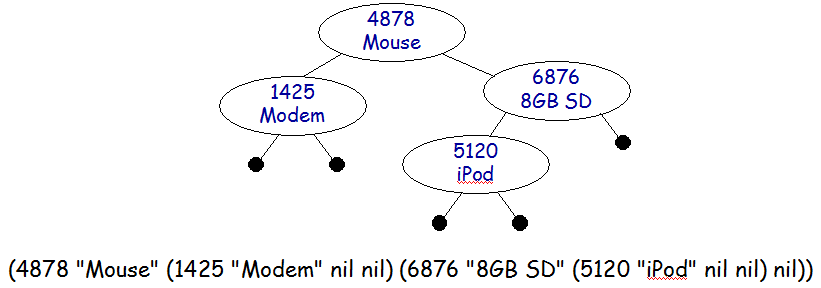
\includegraphics[scale=0.5]{images/searchtree.png}
\end{center}
\caption{Search Tree Diagram and Corresponding Formula}
\label{fig:searchtree-diagram}
\end{figure}

\label{height-def}
The height of an empty tree is zero.
The height of a non-empty tree is one more than that of the
taller of its left and right subtrees.
The size of a search tree is the number of keys that occur in the tree,
which is zero for an empty tree, and
for a non-empty tree, is one more than the sum
of the sizes of its left and right subtrees.

We use ACL2 to formalize these definitions
(Figure \ref{fig:tree-functions}, page \pageref{fig:tree-functions}),
starting with an operator to build a tree from its four components.
Then we define operators to extract keys, data, and subtrees from nodes
(key, dat, lft, and rgt).
Finally, we define predicates to recognize keys and search trees
(iskeyp, treep, emptyp),
and to find out whether a key occurs in a tree (keyp).

\begin{figure}
\begin{center}
\begin{Verbatim}
(defun mktr (k d lf rt)            ; make tree from
  (list k d lf rt))                ;  key, data, subtrees
(defun key (s) (first s))          ; key at root
(defun dat (s) (second s))         ; data at root
(defun lft (s) (third s))          ; left subtree
(defun rgt (s) (fourth s))         ; right subtree
(defun emptyp (s) (not (consp s))) ; empty tree?
(defun height (s)                  ; tree height
  (if (emptyp s)
      0                                               ; ht0
      (+ 1 (max (height (lft s)) (height (rgt s)))))) ; ht1
(defun size (s)                    ; number of keys
  (if (emptyp s)
      0                                     ; sz0
      (+ 1 (size (lft s)) (size (rgt s))))) ; sz1
(defun n-element-list (n xs)
  (if (zp n)
      (equal xs nil)
      (and (consp xs) (n-element-list (- n 1) (rest xs)))))
(defun iskeyp (k)                ; keys are natural numbers
  (natp k))
(defun treep (s)                 ; search tree?
  (or (emptyp s)
      (and (n-element-list 4 s) (iskeyp (key s))
           (treep (lft s)) (treep (rgt s)))))
(defun keyp (k s)                ; key k occurs in s?
  (and (iskeyp k) (treep s) (not (emptyp s))
       (or (= k (key s))
           (keyp k (lft s))
           (keyp k (rgt s)))))
\end{Verbatim}
\end{center}
\caption{Search Tree Operators and Predicates}
\label{fig:tree-functions}
\end{figure}

The only tree of height zero is the empty tree because
the height of a non-empty tree is one more than the maximum
of two other numbers, which makes it at least one.
Theorem \{\emph{ht-emp}\} states this fact more rigorously.

\label{thm:ht-emp}
Theorem \{\emph{ht-emp}\} (treep $s$) $\rightarrow$ (((height $s$) = 0) = (emptyp $s$))
\section{Ordered Search Trees}

Since keys are natural numbers,
search trees are ordered (page \pageref{ordered-def}) if, for each node,
its key is greater than all of the keys that occur in the left subtree
and less than all the keys that occur in the right subtree.
A empty tree is ordered by default.
The following equations of predicate calculus define
``ordp'' so that
(ordp $s$) is true if $s$ is ordered and false otherwise.

\begin{center}
\label{def:ordp}
\begin{tabular}{lll}
(ordp nil) = & true & \{\emph{ord0}\} \\
(ordp $s$) = & (treep s)  $\wedge$                                                                                     & \{\emph{ord1}\} \\
             & ($\forall x$.((keyp $x$ (lft $s$)) $\rightarrow$ $x$ < (key $s$))) $\wedge$ (ordp (lft $s$)) $\wedge$ & \\
             & ($\forall y$.((keyp $y$ (rgt $s$)) $\rightarrow$ $y$ > (key $s$))) $\wedge$ (ordp (rgt $s$))          & \\
\end{tabular}
\end{center}

Duplicate keys do not occur in ordered search trees.
A more rigorous statement of this fact can be based on
the following observations:
\begin{quote}
\begin{enumerate}
\item A key in a node does not occur in either of its subtrees.
\item Any key in one subtree of a node is not equal to the node's key
      and doesn't occur in the other subtree.
\end{enumerate}
\end{quote}

\begin{quote}
\label{thm:keys-unique}
Theorem \{\emph{keys unique}\}. \\
((iskeyp $k$) $\wedge$ (ordp $s$)) $\rightarrow$ \\
((($k$ = (key $s$)) $\rightarrow$ ((not(keyp $k$ (lft $s$))) $\wedge$ (not(keyp $k$ (rgt $s$))))) $\wedge$ \\
(((keyp $k$ (lft $s$))) $\rightarrow$ (($k$ $\ne$(key $s$)) $\wedge$ (not(keyp $k$ (rgt $s$))))) $\wedge$ \\
(((keyp $k$ (rgt $s$))) $\rightarrow$ (($k$ $\ne$(key $s$)) $\wedge$ (not(keyp $k$ (lft $s$)))))) \\
\end{quote}

Stating this theorem is more complicated than proving it.
The proof simply applies the definition of ordp judiciously in each circumstance.
For example, if $k$ = (key $s$), then (keyp $k$ (lft $s$)) must be false
because if (keyp $k$ (lft $s$)) were true, then $k$ $<$ (key $s$),
according to the definition of ordp. That is inconsistent with  $k$ = (key $s$),
so (keyp $k$ (lft $s$)) must be false
(\{\emph{reductio ad absurdum}\},
Figure \ref{fig-02-deduction-rules}, page \pageref{fig-02-deduction-rules}).
By a similar argument, (keyp $k$ (lft $s$)) also must be false.
So, the first operand of the $\wedge$ formula of the theorem is true.
Proving that the other two operands are also true can be done
with similar reasoning from the definition of ordp.
Since each operand of the $\wedge$ formula is true when the hypothesis
of the implication (ordp $s$) is true,
the implication formula that comprises the theorem is true
(\{$\wedge$ implication\}, page \pageref{and-implication})

\begin{ExerciseList}
\Exercise Verify:
(ordp $s$) $\rightarrow$ (((keyp $k$ (lft $s$))) $\rightarrow$ (($k$ $\ne$(key $s$)) $\wedge$ (not (keyp $k$ (rgt $s$)))))

\Exercise Verify:
(ordp $s$) $\rightarrow$ (((keyp $k$ (rgt $s$))) $\rightarrow$ (($k$ $\ne$(key $s$)) $\wedge$ (not (keyp $k$ (lft $s$)))))
\end{ExerciseList}

\section{Balanced Search Trees}

Search trees must be ordered to make it convenient to find things.
However, order is not enough.
Trees must also be short, relative to the number of items in the tree.
Otherwise, order doesn't help.
It can take as long, on the average, to find an item
in an ordered but unbalanced tree as it would
if the data were completely unorganized.
Figure \ref{fig:unbalanced-trees} (page \pageref{fig:unbalanced-trees})
compares some extremes.

\begin{figure}
\begin{center}
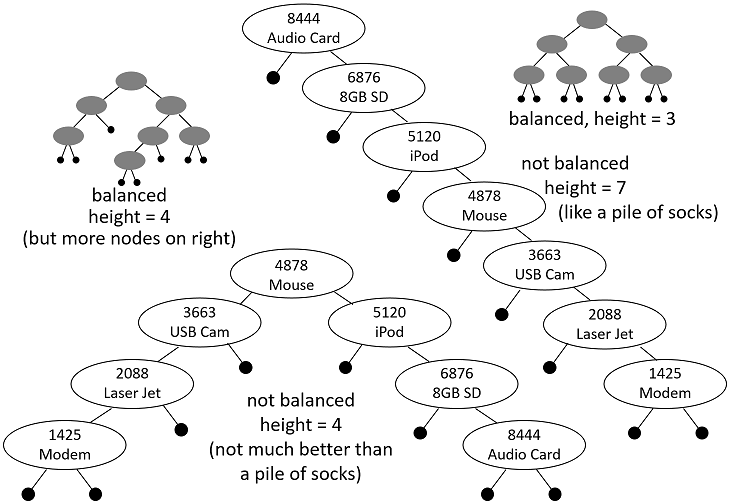
\includegraphics[scale=0.5]{images/unbalanced-trees.png}
\end{center}
\caption{Balance Shortens Trees}
\label{fig:unbalanced-trees}
\end{figure}

The tree of height seven in
Figure \ref{fig:unbalanced-trees} (page \pageref{fig:unbalanced-trees})
is unbalanced at every level.
A binary search on this tree would have no advantage over
looking through a pile of socks, one by one.
The tree of height four in the figure is not much better.
It has the name number of nodes in the left subtree as in the right subtree,
but all of the subtrees are maximally unbalanced, like a pile of socks.

Balance is what prevents time-consuming searches like the ones in
extreme cases shown.
A search tree that, in every node, has two subtrees of the same size
is balanced in terms of both size and height. The tree of height three
in Figure \ref{fig:unbalanced-trees} (page \pageref{fig:unbalanced-trees})
has this maximally balanced shape.
However, the number of steps
required to find a key in a search tree is determined by the heights of subtrees,
not the number of nodes they contain, and
a tree can be balanced with respect to height even though some nodes contain
many more keys in one subtree than the other.
The tree of height four in the figure shows how this can happen.
The shape of this tree isn't symmetric at any level,
but no node has subtrees whose heights differ by more than one,
and that's good enough.
We are trying keep the height of a tree with $n$ nodes
within a fixed percentage of $log(n)$,
and height balancing is sufficient to accomplish this goal.
Full symmetry isn't necessary.

As we mentioned before (page \pageref{50pct-thm})
the height of a balanced search tree
turns out to be less than $1.5 \cdot log_2(n)$.
That makes finding things take a few more
steps than the optimal case in which both subtrees of
each node contains the same number keys,
but the number of steps in the search is still small.
Finding a particular key among a billion nodes
might require 45 steps instead of 30, but that's
still plenty fast compared with half a billion steps,
on the average, for unorganized data.

What we get for a few extra steps in finding things is
an astonishing improvement in the number of steps required
to insert a new key or delete an old key.
Instead of $n/2$ steps, on the average,
using arrays in which the keys beyond the point of insertion
all need to be moved to make space for the new one,
insertion can be done in logarithmic time.
That is, the number of steps required to to insert
a node in a search tree will be proportional to $log(n)$,
giving us the same advantage in insertion speed
that binary search provides in look-up speed.
Deletion can be handled in a similar way, and with the same effectiveness.
That is, search, insertion, and deletion can all be done in logarithmic time.

\begin{ExerciseList}
\Exercise Prove that it is possible to put $2^n - 1$ keys
in a binary tree of height $n$.
\end{ExerciseList}

\section{Inserting a New Item in a Search Tree}

To make search, insertion, and deletion efficient,
search trees must be both ordered and balanced.
We regard to balance,
we must make sure that both subtrees
of any node in a search tree have the same height, or that the
height of one of them is only one more than the height of the other.
\label{balance-def}
The predicate ``balp'' expresses this notion formally
(Figure \ref{fig:balance-defun}, \pageref{fig:balance-defun}).

\begin{figure}
\begin{center}
\begin{Verbatim}
(defun balp (s) ; tree s is balanced?
  (or (emptyp s)
      (and (<= (abs (- (height (lft s)) (height (rgt s)))) 1)
           (balp (lft s) (balp (rgt s))))))
\end{Verbatim}
\end{center}
\caption{Balance Predicate}
\label{fig:balance-defun}
\end{figure}

It isn't difficult to maintain order.
You can do this by moving left or right down the tree according
to whether the new key is less than or greater than the key in the node
under consideration.
When you arrive at an empty tree,
make a new tree like the old one, but
with a node at that point that has,
as its key, the new key (and its associated data),
and  put in empty trees for the new node's left and right subtrees.
The new tree will be properly ordered because
of the way the procedure located a place to
hook the new key,
but the new tree will not be balanced if
the location of the new key increases the height
of a subtree that was already one taller than its sibling.

Figure \ref{fig:hook-defun} (\pageref{fig:hook-defun}) provides
an inductive definition of this key insertion method.
The definition uses a non-inductive formula
to put the new key into an empty tree
and an inductive formula for the non-empty case.\footnote{In
\label{same-key-new-data}
case the operator,
hook, encounters a key that is the same
as the one it is inserting, it delivers a tree with that key, as it should.
However, the data associated with the new key will be the data supplied
as the second argument in the invocation of hook.
The old data is lost.
The definition might have chosen a different alternative
in the case of equal keys. This choice
provides a way to associate new data with a key.}

\begin{figure}
\begin{center}
\begin{Verbatim}
(defun hook (x a s) ; put a new key x with data a into tree s
  (if (empty s)     ; preserve order, but not necessarily balance
      (mktr x a nil nil)
      (let* ((k  (key s)) (d (dat s))
             (lf (lft s)) (rt (rgt s)))
        (if (< x k)
            (mktr k d (hook x a lf) rt)      ; hook<
            (if (> x k)
                (mktr k d lf (hook x a rt))  ; hook>
                (mktr x a lf rt))))))        ; hook=
\end{Verbatim}
\end{center}
\caption{Insert New Key, Preserving Order, but Not Balance}
\label{fig:hook-defun}
\end{figure}

Inserting a new key in this way
can throw the tree out of balance.
That happens when
placement of the new key increases the height of a subtree that was
already taller than its sibling.
Then the subtree will be two units taller than its sibling,
making the tree unbalanced.
In this case, a rearrangement will bring it back into balance
without getting keys out of order.
In small trees, it's easy to find an ad hoc rearrangement that works,
as illustrated in Aside \ref{aside:insertion-example}
(page \pageref{aside:insertion-example}),
but we need a procedure that works for all search trees,
not just small ones where we can see what to do.
Figuring out a rearrangement procedure is what the rest
of this chapter is mostly about.

\begin{aside}
The following example starts with a tree containing one item,
then inserts three new items, one at a time.
We use the formula (ins $x$ $a$ $s$) to denote
the tree produced by inserting the key $x$ and associated
data $a$ into the search tree $s$.

The end result is an ordered,
balanced tree containing four items.
It will aid your understanding
of the insertion process if you draw diagrams similar to Figure
\ref{fig:unbalanced-trees} for the trees denoted by the formulas in the example.
Verify, as you go, that each tree is both ordered and balanced.
\begin{center}
\begin{tabbing}
%
\vspace*{-1.5\topsep}
\rule{\textwidth}{0.4pt}
\vspace*{-\topsep}
%
\\
(ins \= 1125 "Modem" \\
     \> {[}8444 "Audio Card" nil nil{]}) \\
     \> $\Downarrow$ \\
{[}1125 "Modem" nil {[}8444 "Audio Card" nil nil{]}{]} \\
%
\vspace*{-1.5\topsep}
\rule{\textwidth}{0.4pt}%
\vspace*{-\topsep}
%
\\
(ins \= 4878 "Mouse" \\
     \> {[}1125 "Modem" nil {[}8444 "Audio Card" nil nil{]}{]}) \\
     \> $\Downarrow$ \\
{[}4878 "Mouse" \= {[}1125 "Modem"      nil nil{]}  \\
              \> {[}8444 "Audio Card" nil nil{]}{]} \\
%
\vspace*{-1.5\topsep}
\rule{\textwidth}{0.4pt}%
\vspace*{-\topsep}
%
\\
(ins \= 2088 "Laser Jet" \\
     \> {[}4878 "Mouse" \= {[}1125 "Modem" nil nil{]} \\
     \>               \> {[}8444 "Audio Card" nil nil{]}{]}) \\
     \> $\Downarrow$ \\
{[}2088 "Laser Jet" \= {[}1125 "Modem" nil nil{]} \\
                  \> {[}4878 "Mouse" nil {[}8444 "Audio Card" nil nil{]}{]}{]} \\
%
\vspace*{-1.5\topsep}
\rule{\textwidth}{0.4pt}%
\vspace*{-\topsep}
%
\end{tabbing}
\end{center}

\caption{Inserting New Nodes in Small Trees}
\label{aside:insertion-example}
\end{aside}

Putting the new node at the bottom may make the tree taller,
but not necessarily.
For example the insertion point might be on the
empty side of a node that has a tree of height one on the other side,
which would leave the height of the tree unchanged.
But, if the height of the tree changes,
how much could it change?
Not by more than one
(Theorem \{\emph{i-ht}\}, page \pageref{thm:i-ht}).

If the tree with the new key is taller than the old tree,
the new tree could be unbalanced.
However, because a height of the left subtree of a
balanced tree does not differ from the height of
the right subtree by more than one,
and because the insertion of a new node cannot increase
the height of either subtree by more than one,
the heights of the left and right subtrees in the new tree
cannot differ by more than two.
So, if we can figure out how to rebalance trees where
one subtree is two units taller than its sibling,
we will have found a way preserve balance
while inserting a new node.

\begin{ExerciseList}
\Exercise Given any three distinct keys,
there is only one search tree that is ordered, balanced
and contains those three keys but no others.
Explain why.

\Exercise Aside \ref{aside:insertion-example}
(page \pageref{aside:insertion-example}) displays
insertions leading to an ordered, balanced search tree
containing four items.
The resulting trees were chosen from several, equally suitable alternatives.
Write formulas for ordered, balanced trees different from
the ones in the example that contain the same keys.

\Exercise Prove by induction on tree height
that insertion of a new node does not increase height by more than one.
That is, assuming that $x$ is a key, $s$ is a search tree,
and hook is the operator defined in
Figure \ref{fig:hook-defun} (page \pageref{fig:hook-defun}),
prove the following theorem.
\begin{center}
\label{thm:i-ht}
Theorem \{\emph{i-ht}\}: (height $s$) = $n$ $\rightarrow$ (height (hook $x$ $a$ $s$)) $\leq n+1$
\end{center}

\Exercise Use induction on height to prove the following theorem
(ordp is defined on page \pageref{def:ordp}).
\begin{center}
\label{thm:i-ord}
Theorem \{\emph{i-ord}\}
(ordp $s$) $\rightarrow$ (ordp (hook $x$ $a$ $s$))
\end{center}

\end{ExerciseList}

\section{Insertion, Case by Case}
Balancing small trees is easy because there are only a few
possibilities to consider. Search trees of height two or less
are always balanced.
\begin{center}
\label{thm:bal-ht2}
Theorem \{\emph{bal-ht2}\}. (height $s$) $\leq 2$) $\rightarrow$ (balp $s$).
\end{center}

Working through all the possibilities, one by one,
leads to a proof of this theorem.
A tree of height zero is empty
(Theorem \{\emph{ht-emp}\}, page \pageref{thm:ht-emp}),
and (balp nil) = (emptyp nil) is true, by definition
(Figure \ref{fig:balance-defun}, page \pageref{fig:balance-defun}).
Any tree of height one will consist of a single node,
[$k$ $d$ nil nil], which is balanced because both subtrees
have the same height (namely, zero).
The formula for a tree of height two must match one of the following templates:
[$k$ $d$ [$j$ $c$ nil nil] nil], [$k$ $d$ nil [$i$ $b$ nil nil]],
or [$k$ $d$ [$j$ $c$ nil nil] [$i$ $b$ nil nil]].
Applying the predicate balp
confirms that all of these trees are balanced,
and that completes the proof of Theorem \{\emph{bal-ht2}\}.

With big trees, there are more possibilities,
but we can reduce part of the problem to
a shorter tree, rely on induction to deal with that tree,
and use the solution produced on the shorter tree
to put together a full solution.
We want to define an insertion operator ``ins''
to put a new key in
an ordered, balanced search tree,
producing a new search tree that is ordered, balanced,
and contains the new key as well as all of the old ones.
The operator hook (Figure \ref{fig:hook-defun}, page \pageref{fig:hook-defun})
does the job for trees of height zero or one.
The new tree is ordered (Theorem \{\emph{i-ord}\}, page \pageref{thm:i-ord})
and being of height two or less, it is also balanced
(Theorem \{\emph{i-ht}\}, page \pageref{thm:i-ht},
together with Theorem \{\emph{bal-ht2}\}, page \pageref{thm:bal-ht2}).
So, for trees of height zero or one,
we can use the procedure defined in hook
to insert new keys.

That leaves us with trees of height two or more.
We want to define an insertion operator, ins,
so that
if $s$ is an ordered, balanced search tree
of height $n+2$ (where $n$ is a natural number),
then the tree (ins $x$ $a$ $s$)
is ordered, balanced, contains all the keys in $s$,
contains the key $x$,
contains no keys other than $x$ and those in $s$,
and has height $n+2$ or $n+3$.
To do this,
we will start with the hook procedure
(which has, already, the order and height properties
that we need for ins),
then find ways to rebalance when it produces
a tree with subtrees whose heights differ by more than one.\footnote{Our
primary concerns will be the issues of height and balance.
The other issues
(presence of the new key, preservation of all the old keys,
etc.)
are easy to work through from the definitions.
An issue that we will gloss over throughout the discussion
is the treatment of data associated with a key.
We include the data in the operator definitions because,
as a practical matter, search trees need some way to
associate data with keys.
Usually, keys just provide a way to find the data.
The operator definitions take care to keep each data item
with its associated key.
Whenever we use mktr to build a tree,
we put the key in the first argument
and the associated data in the second argument.
This keeps the key with its data.
However, that is pretty much the extent of
our analysis of key/data associations.
Doing more is tricky because there are no
constraints on the domain of the data.
The data could even come from a domain
that doesn't support reasoning about equality.
This would be the case, for example, if the data items
were, themselves, operators, and the search tree
were being used to provide organized access to those
operators. There is no algorithm
for determining, in general, whether two operators
denote the same operation,
so it would be difficult to reason about whether or
not key/data associations stay the same throughout the process.}
Our inductive definition of ins will
assume that it has the desired properties
when operating on trees of height less than $n+2$
and prove that, with that assumption, it also
has those properties on trees of height $n+2$.

\begin{figure}
\begin{center}
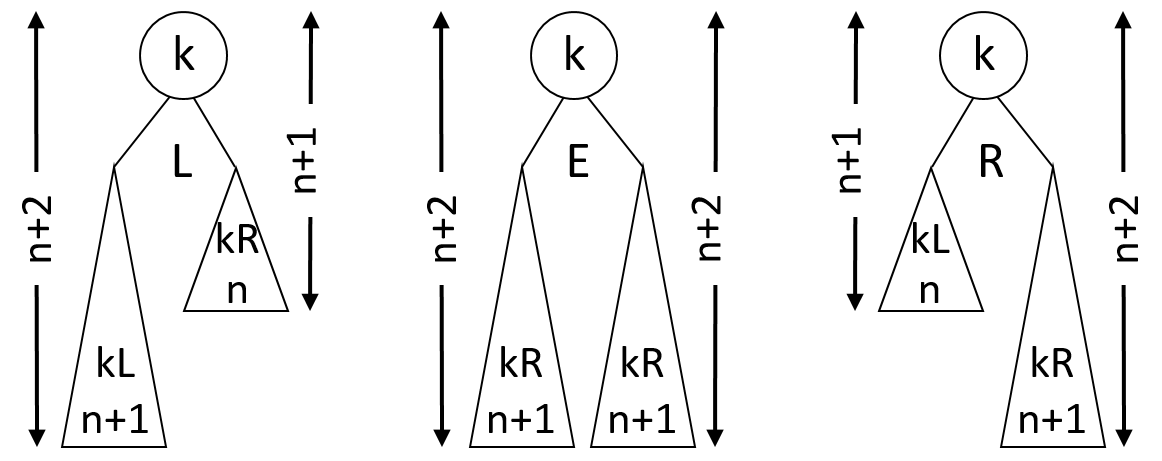
\includegraphics[scale=0.5]{images/ht2-or-more.png}
\end{center}
\caption{Balanced Trees of Height $n+2$}
\label{fig:trees-of-ht-n+2}
\end{figure}

Diagrams of search trees will help us work through the analysis, case by case.
Figure \ref{fig:trees-of-ht-n+2} (page \pageref{fig:trees-of-ht-n+2})
displays the three configurations that a search tree of height $n+2$ can have.
Each diagram shows the root node as a circle labeled with a name for its key
and shows the left and right subtrees as triangles dangling from the root.
Each triangle represents an ordered, balanced subtree.
A label in the middle of the triangle
simplifies references to the subtree,
and a formula near the bottom of the triangle
specifies the height of the subtree.
Each tree as a whole is labeled with a name near the top of its diagram
(\emph{L}, \emph{E}, and \emph{R}).
The tree \emph{L} is one unit taller on the left than on the right,
\emph{R} is taller on the right, and
both subtrees in \emph{E} have the same height.

An insertion into tree \emph{E} cannot cause the tree to go out of balance
because, at worst, insertion will make one side of the tree
one unit taller than the other side, and leaves the tree
balanced. (The subtrees have height less than $n+2$,
so the induction hypothesis guarantees that they remain
balanced after insertion.)
Therefore, we do not concern ourselves with trees like \emph{E}.
However, if we insert a new key that is less than $k$
into tree \emph{L}, the key would end up in subtree \emph{kL},
the left subtree of \emph{L}, and
the tree could go out of balance
because the height of its left subtree could increase to $n+2$,
while the right subtree would remain at height $n$.
Similarly, inserting a key greater than $k$ into the tree \emph{R}
could make its right subtree \emph{kR} too tall.
Tree \emph{L} and tree \emph{R} represent the cases we need to look into.

\begin{figure}
\begin{center}
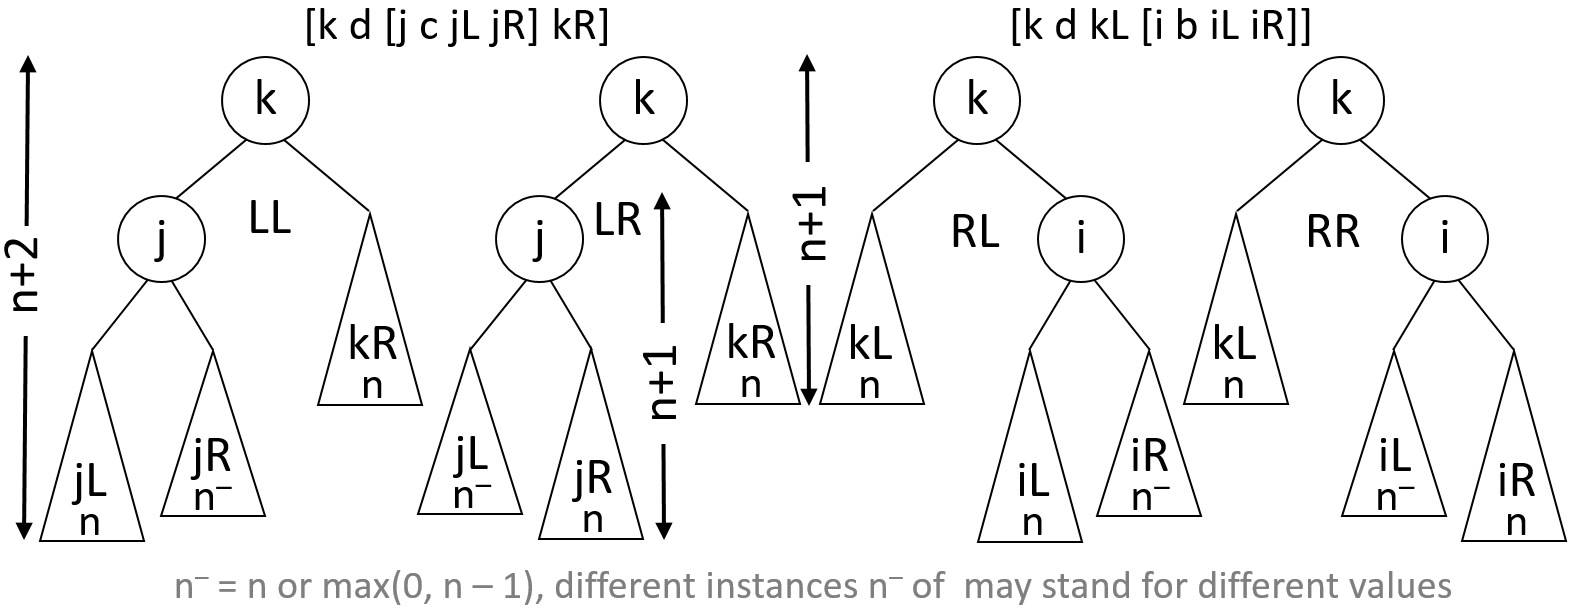
\includegraphics[scale=0.5]{images/ht2-or-more-ex.png}
\end{center}
\caption{Balanced Trees of Height $n+2$, Subtrees Expanded}
\label{fig:trees-of-ht-n+2-expanded}
\end{figure}

Figure \ref{fig:trees-of-ht-n+2-expanded} (page \pageref{fig:trees-of-ht-n+2-expanded})
will guide deeper analysis.
In the figure, certain subtrees of \emph{L} and \emph{R} from
Figure \ref{fig:trees-of-ht-n+2} (page \pageref{fig:trees-of-ht-n+2})
are expanded to show additional details.
The new diagrams expand subtree
\emph{kL} in tree \emph{L} and subtree \emph{kR} in tree \emph{R}.
Both of these subtrees have height $n+1$.
That makes them non-empty, so each of them must have at least one key.
The expanded diagrams of these subtrees
reveal details about their keys and subtrees.

In tree \emph{L} (Figure \ref{fig:trees-of-ht-n+2}),
the subtree \emph{kL} has height $n+1$,
so at least one of its subtrees has height $n$.
Its sibling might also have height $n$, but (unless $n$ is zero)
it could alternatively have height $n-1$.
The diagrams in Figure \ref{fig:trees-of-ht-n+2-expanded}
and other diagrams in this chapter
use the notation $n^-$
to denote a value that could be either $n$
or, if $n$ isn't zero, $n-1$.
The value denoted by $n^-$ is not necessarily the same
in all of the tree diagrams in the figure,
but the value will be, in every instance,
either $n$ or $n-1$.

Either subtree may be the taller one,
so we draw two diagrams representing the two possibilities
(trees \emph{LL} and \emph{LR}).
Similarly, there are two diagrams for the tree \emph{R},
which makes a total of four tree diagrams in
Figure \ref{fig:trees-of-ht-n+2-expanded}:
two diagrams (\emph{LL} and \emph{LR})
expanding tree \emph{L} from Figure \ref{fig:trees-of-ht-n+2}
and two diagrams (\emph{RL} and \emph{RR}) expanding tree \emph{R}.

Consider the problem of inserting a new key, $x$, into
an ordered, balanced search tree of height $n+2$.
The value of $x$ will fall into one of four intervals\footnote{We
can ignore the possibility that $x$ is the same as
$k$, $j$, or $i$ because
inserting a key that is the same as one already in the
tree does not change the tree,
except to replace the data associated with the key.
Therefore, the tree will remain balanced and
require no further attention.}:
\begin{quote}
\begin{enumerate}
\label{cases:ht-n+2}
\item case \emph{LL}: $x < j$ (refer to Figure \ref{fig:trees-of-ht-n+2-expanded})
\item case \emph{LR}: $j < x < k$
\item case \emph{RL}: $k < x < i$
\item case \emph{RR}: $i < x$
\end{enumerate}
\end{quote}

The names of the cases correspond
to the tree diagram in
Figure \ref{fig:trees-of-ht-n+2-expanded} (page \pageref{fig:trees-of-ht-n+2-expanded})
that we will use for analysis of the case.
For example, if the new key $x$ is less than $k$,
insertion cannot cause the tree to go out of
balance unless the left subtree is taller
than the right subtree, which focuses the
analysis on trees \emph{LL} and \emph{LR}
in Figure \ref{fig:trees-of-ht-n+2-expanded}.
We use \emph{LL} for the case when $x < j$
because that pushes the key into subtree \emph{jL},
and the tree \emph{LL} will definitely go out of balance
if insertion increases the height of \emph{jL}.
The same insertion might not cause the tree \emph{LR}
to go out of balance, even if it increases the height of
the subtree \emph{jL}, because in tree \emph{LR}
the subtree \emph{jL} may be shorter
than its sibling, \emph{jR}.
If not, then the situation is covered already in case \emph{LL}.
For similar reasons, we use the diagrams
of \emph{LR}, \emph{RL}, and \emph{RR}
to analyze their namesake cases.

Case \emph{LL} is the problem of inserting
a key $x$ that is less than $j$
into the tree \emph{LL}.
The new key will go into the subtree \emph{jL}.
Since the height, $n$, of \emph{jL} is less than $n+2$,
the induction hypothesis says that the new subtree,
after insertion,
will be balanced and have height $n$ or $n+1$.
If it has height $n$, the tree, as a whole, remains
balanced, and nothing further needs to be done.
If it has height $n+1$, the tree, as a whole,
will be out of balance (too tall on the left).
It will need rebalancing.

\begin{figure}
\begin{center}
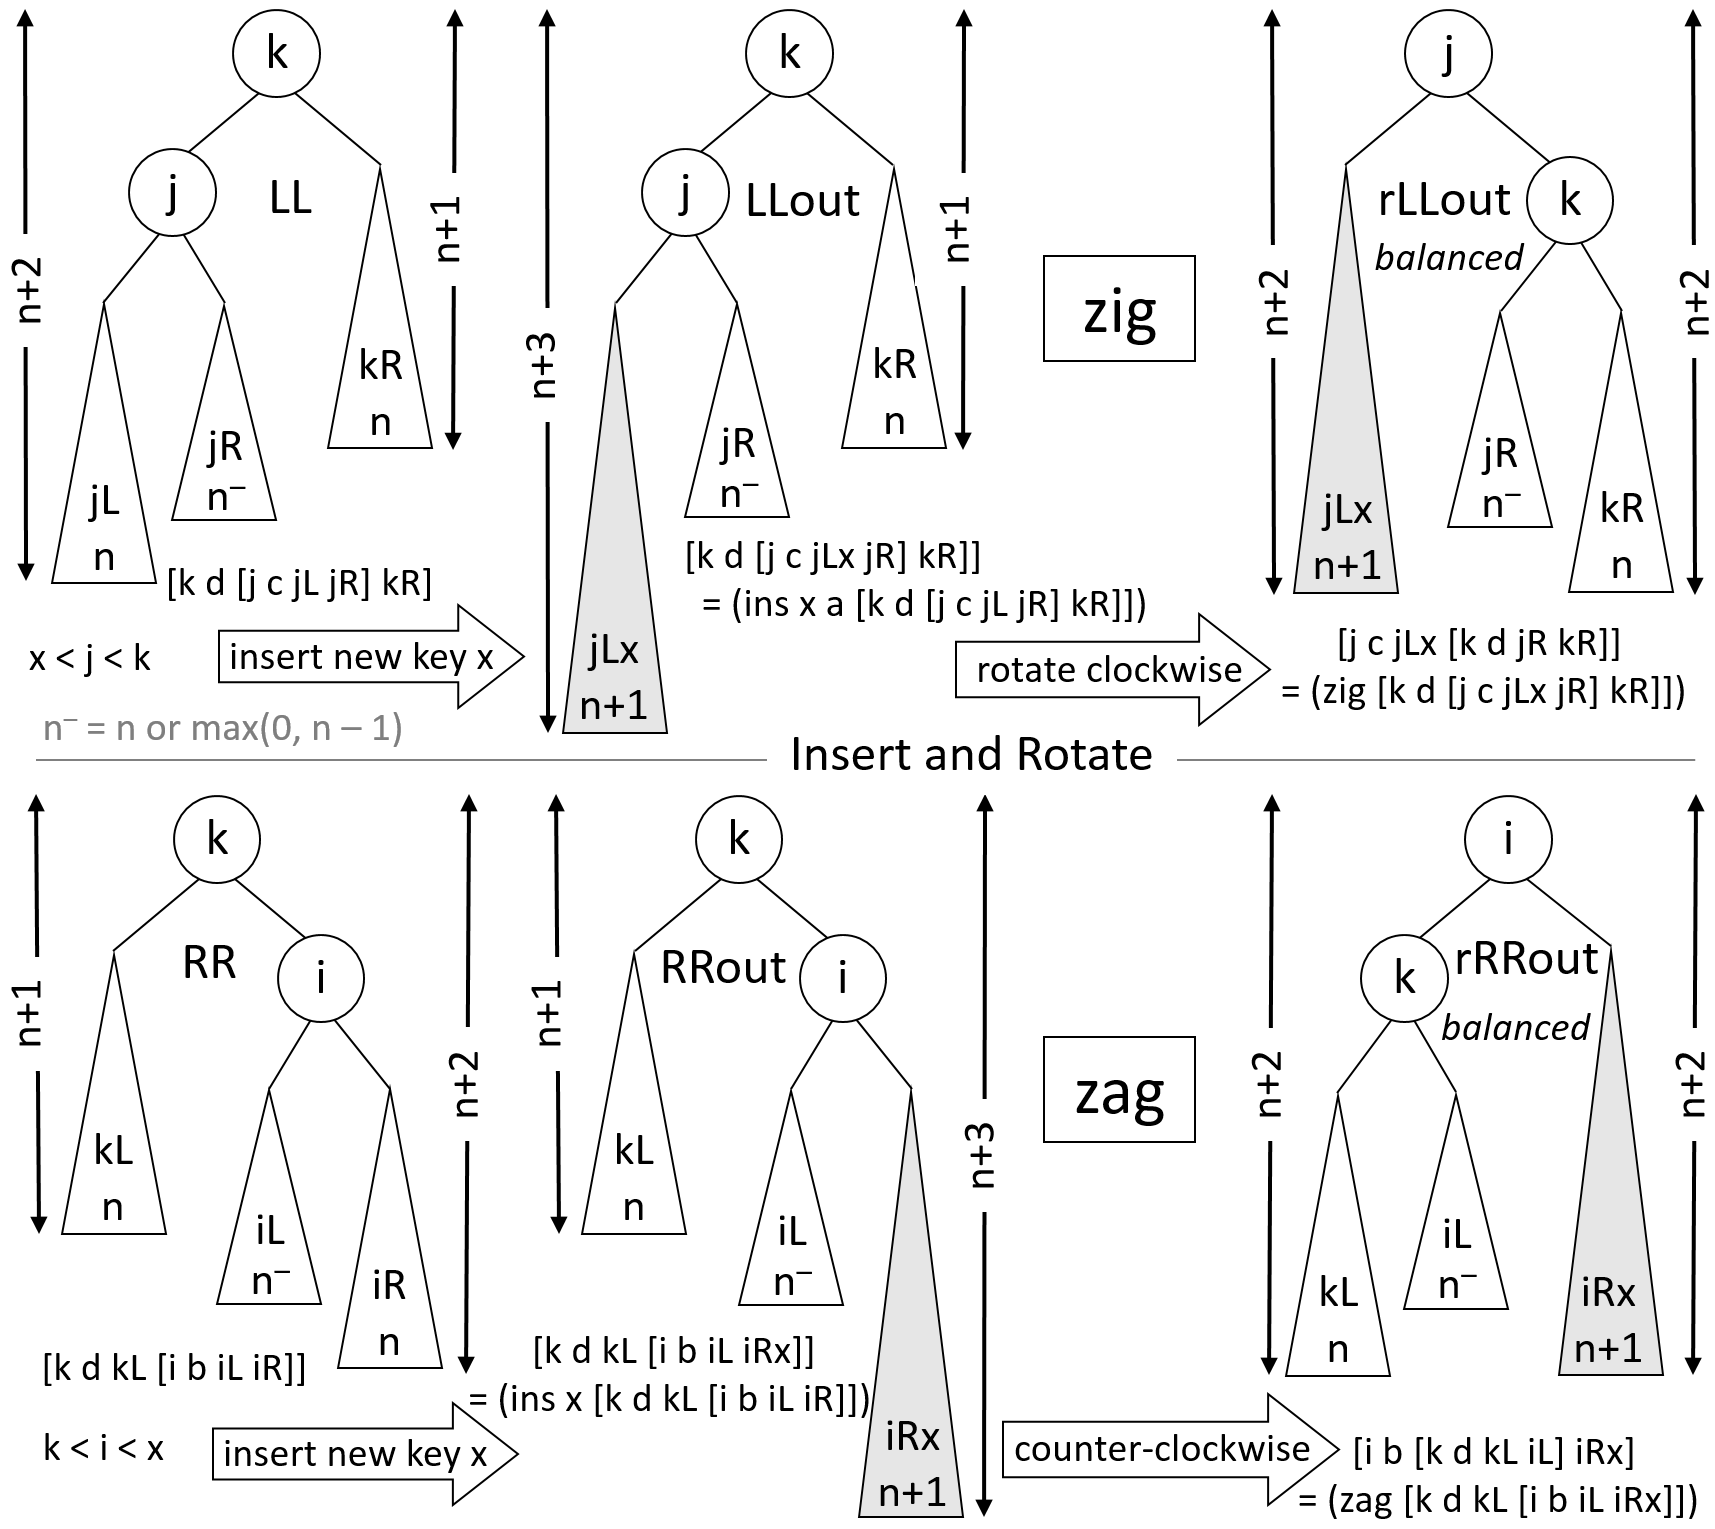
\includegraphics[scale=0.38]{images/zig-and-zag.png}
\end{center}
\caption{Insertion, Unbalanced Outcome, and Rebalancing}
\label{fig:zig-and-zag}
\end{figure}

Figure \ref{fig:zig-and-zag} (page \pageref{fig:zig-and-zag})
displays the tree \emph{LL} before insertion
(as it appeared in Figure \ref{fig:trees-of-ht-n+2-expanded})
and a new, unbalanced tree, \emph{LLout}, which represents
the outcome of inserting a new key $x$ ($x < j$) into \emph{LL}.
In the diagram of \emph{LLout}, the subtree
\emph{jLx} is the one with the new key.
The subtree \emph{jLx} has height $n+1$,
which makes \emph{LLout} too tall on the left.
Figure \ref{fig:zig-and-zag} also presents the mirror insertion
into \emph{RR} of a key
$x$ ($i < x$),
producing a tree labeled \emph{RRout}
that is too tall on the right.

Because these insertions lead to unbalanced trees,
we need to rearrange them in some way,
and Figure \ref{fig:zig-and-zag} shows how to do that.
In the case of \emph{LLout},
the key $j$ can go at the root, and the former root key, $k$,
can hang from the right side of the new root.
If we then plug the subtrees into the only places they
can go that preserves order,
the result, tree\emph{rLLout} (Figure \ref{fig:zig-and-zag}),
is balanced and has height $n+2$.
Voila! Like magic.

This clockwise rotation of the the tree \emph{LLout},
as shown in the figure,
is traditionally called ``zig''.
The mirror operation, zag, rotates counter-clockwise to fix
the tree \emph{RRout}, which is too tall on the right.
Formal definitions of these rotation operators reside in
Figure \ref{defun:zig-and-zag} (page \pageref{defun:zig-and-zag}).
These definitions emerge in a straightforward way from
the diagrams in Figure \ref{fig:zig-and-zag}.

\begin{figure}
\begin{center}
\begin{Verbatim}
(defun zig (s) ; rotate clockwise
  (let* ((k  (key s)) (d (dat s))
         (j  (key (lft s))) (c  (dat (lft s)))
         (jL (lft (lft s))) (jR (rgt (lft s)))
         (kR (rgt s)))
    (mktr j c jL (mktr k d jR kR))))
(defun zag (s) ; rotate counter-clockwise
  (let* ((k  (key s)) (d (dat s))
         (kL (lft s))
         (i (key (rgt s))) (b (dat (rgt s)))
         (iL (lft (rgt s))) (iR (rgt (rgt s))))
    (mktr i b (mktr k d kL iL) iR)))
\end{Verbatim}
\end{center}
\caption{Rotation Operators: zig and zag}
\label{defun:zig-and-zag}
\end{figure}

The rotation trick fixes unbalanced trees that come
from cases \emph{LL} and \emph{RR} (page \pageref{cases:ht-n+2}).
That leaves us with the other two cases:
case \emph{LR} ($j < x < k$) and
case \emph{RL} ($k < x < i$).
We turn our attention to these problems in the next section.

\begin{ExerciseList}
\Exercise Prove
\label{thm:unbal-ht3}
Theorem \{\emph{unbal-ht3}\}:
If $s$ is an unbalanced tree of height three,
then one subtree of $s$ must be empty and the the other must have height two.
That is, prove the following implication.
\begin{quote}
((height $s$) = 3 $\wedge$ ($\neg$ (balp $s$)))
$\rightarrow$  \\
(((height (lft $s$)) = 2 $\wedge$ (emptyp (rgt $s$)))
$\vee$
((emptyp (lft $s$)) $\wedge$ ((height (rgt $s$)) = 2)))
\end{quote}
\end{ExerciseList}

\section{Double Rotations}

Cases \emph{LR} and \emph{RL} (page \pageref{cases:ht-n+2})
are the only two remaining cases that we need to cover to arrive
at a complete solution of the insertion problem.
The cases we already solved
(cases \emph{LL} and \emph{RR})
are known as the ``outside cases'' because the subtrees that
get the new keys and become too tall are on the outside of the diagram.
Cases \emph{LR} and \emph{RL}
are ``�nside cases'' because the problematic subtrees
are on the inside of the tree diagram:

\begin{center}
\begin{tabular}{llll}
\label{inside-lf} &Inside Left Case \emph{LR}:  &(ins $x$ $a$ \emph{LR}), when $j < x < k$ &
                    (see Figure \ref{fig:trees-of-ht-n+2-expanded}, page \pageref{fig:trees-of-ht-n+2-expanded})                 \\
\label{inside-rt} &Inside Right Case \emph{RL}: &(ins $x$ $a$ \emph{RL}), when $k < x < i$  &
                    \\
\end{tabular}
\end{center}

The inside cases are trickier.
Figure \ref{fig:inside-cases} (page \pageref{fig:inside-cases})
shows how insertions into the trees \emph{LR} and \emph{RL}
can make an inside subtree too tall.

\begin{figure}
\begin{center}
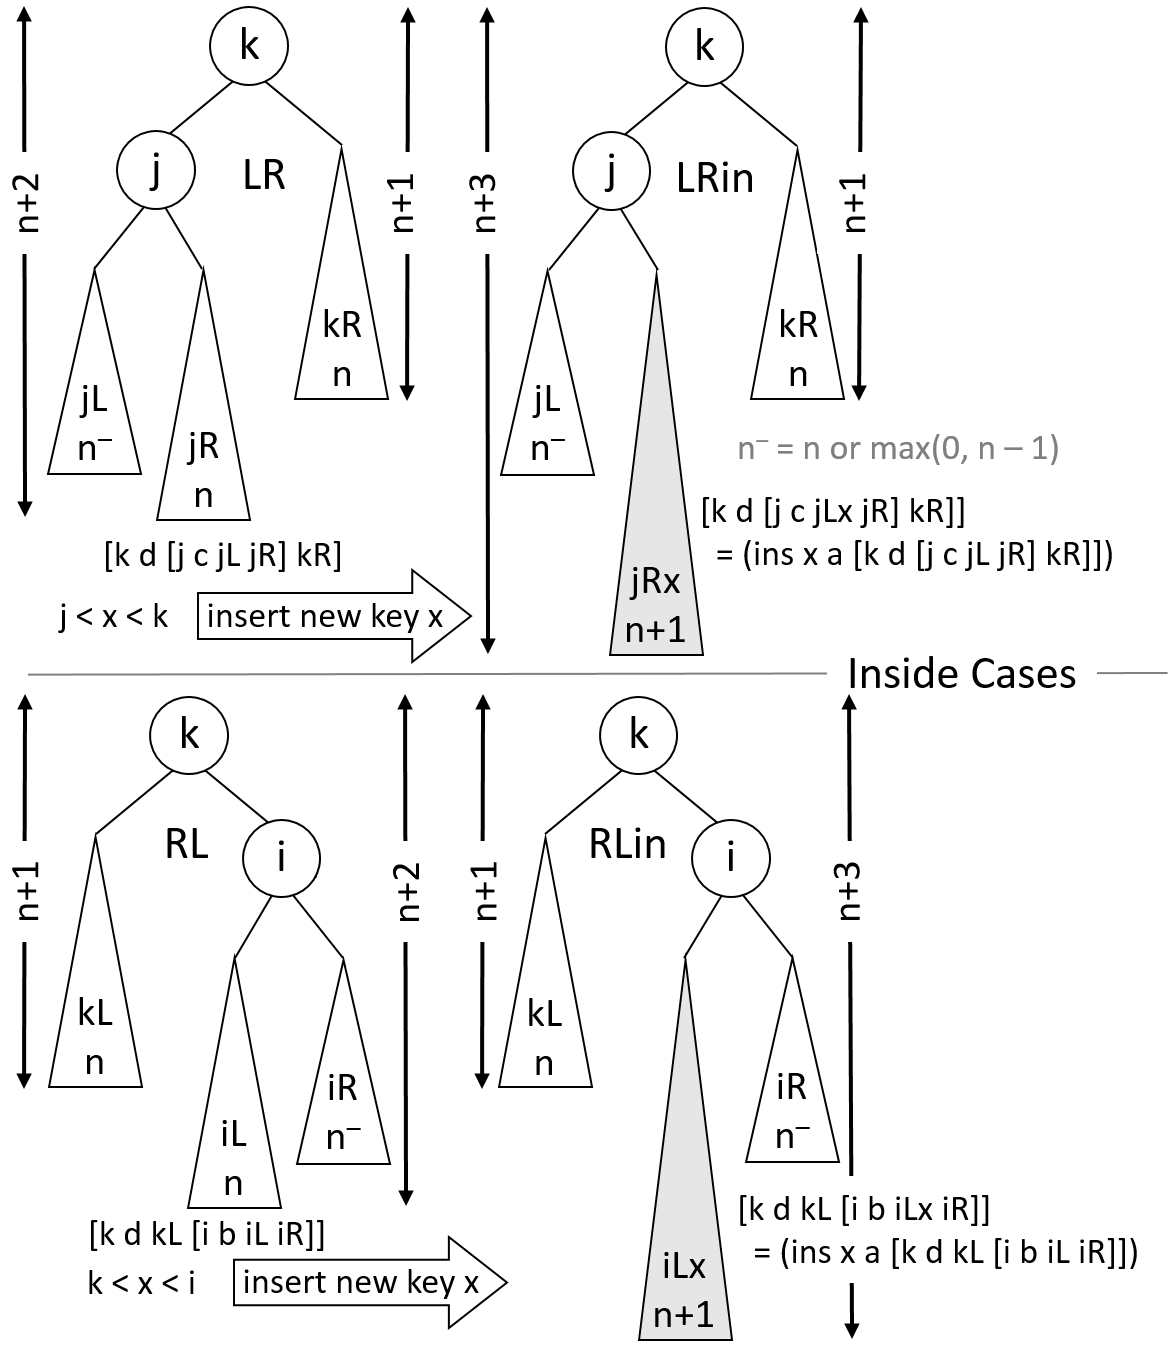
\includegraphics[scale=0.35]{images/inside-cases.png}
\end{center}
\caption{Inside Cases}
\label{fig:inside-cases}
\end{figure}

Consider tree \emph{LRin} in
Figure \ref{fig:inside-cases}.
A first guess might be that the tree \emph{LRin}
could benefit from a clockwise rotation.
However, that produces a tree with a left subtree of height $n$ or $n+1$
and a right subtree of height $n+3$
(see Figure \ref{fig:badzig}, page \pageref{fig:badzig}).
That is, applying the rotation operator, zig, to \emph{LRin}
leads to a tree that is at least as out of balance as \emph{LRin}.
Clockwise rotation doesn't help,
and can make things worse.
We need a new trick to rebalance \emph{LRin}.

\begin{figure}
\begin{center}
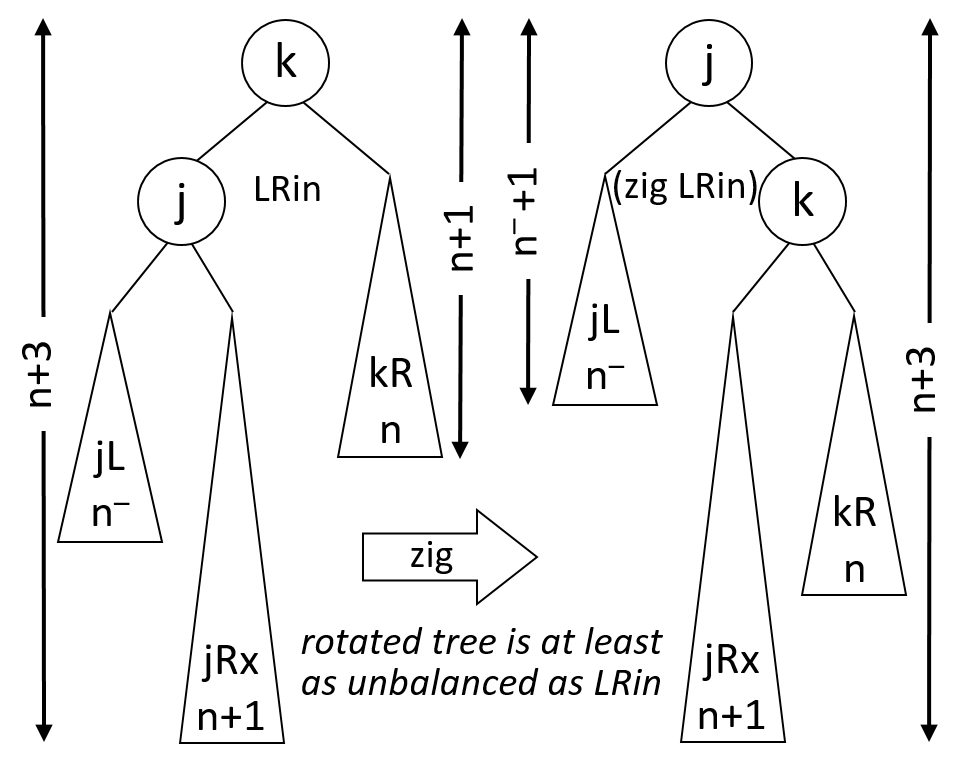
\includegraphics[scale=0.5]{images/badzig.png}
\end{center}
\caption{Using the Wrong Rotation Can Make It Worse}
\label{fig:badzig}
\end{figure}

The height of subtree \emph{jRx}
(Figure \ref{fig:inside-cases}) is $n+1$,
so at least one of its subtrees has height $n$.
The diagram on the left side of
Figure \ref{fig:dbl-rotation} (page \pageref{fig:dbl-rotation})
shows \emph{jRx} expanded to reveal its key $y$,
left subtree \emph{yL}, shown with height $n^-$,
and right subtree \emph{yR}, shown with height $n$.
The heights of those subtrees are either the same,
or \emph{yL} is one unit shorter, but it could
have been the other way around, with
\emph{yL} having height $n$ and \emph{yR}, height $n^-$.
The analysis is the same either way.
We will pursue the alternative
displayed in Figure \ref{fig:dbl-rotation},
and leave it to you to draw the diagram the other way,
just to make sure it all works out.

\begin{figure}
\begin{center}
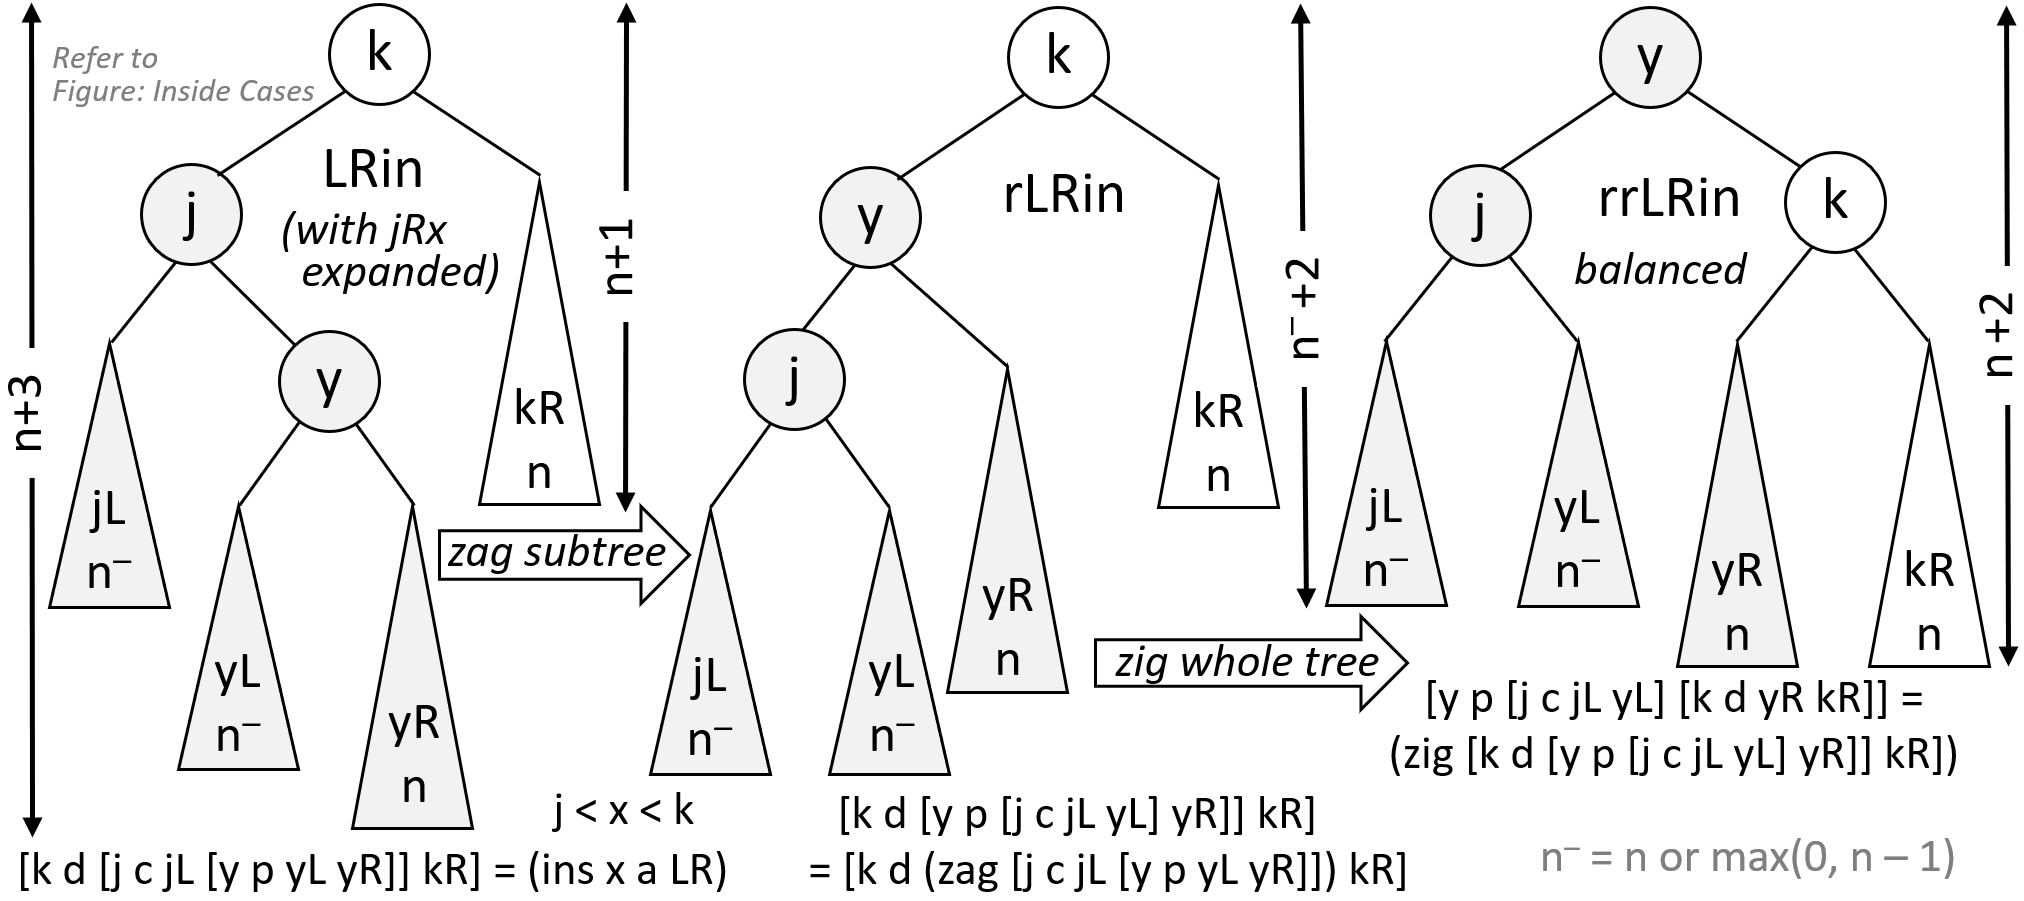
\includegraphics[scale=0.4]{images/dbl-rotation.png}
\end{center}
\caption{Double Rotation Rebalances Inside Cases}
\label{fig:dbl-rotation}
\end{figure}

The diagram makes it clear than we can apply zag
(counterclockwise rotation)
to the left subtree of \emph{LRin}.
It's a counterintuitive move, might not help, might even make things worse,
but it's possible, nonetheless.\footnote{\label{no-zag}It would not be possible
to apply zag if \emph{jRx} were empty.}
When we apply the zag operator to
the left subtree of \emph{LRin},
we get the following result, expressed
using the algebraic formula [$y$ $p$ \emph{yL} \emph{yR}]
for \emph{jRx}.\footnote{The formula uses $p$ to denote
the data associated with the key $y$.}
\begin{center}
(zag (lft \emph{LRin})) =
(zag [$j$ $c$ \emph{jL} [$y$ $p$ \emph{yL} \emph{yR}]]) =
[$y$ $p$ [$j$ $c$ \emph{jL} \emph{yL}] \emph{yR}]
\end{center}

Starting from the unbalanced search tree \emph{LRin}
on the left side of Figure \ref{fig:dbl-rotation},
the middle portion of the figure displays the tree \emph{rLRin},
which is \emph{LRin} with zag applied to its left subtree.
The tree \emph{rLRin},
is not balanced, but the subtree that is too tall
(namely, [$y$ $p$ [$j$ $c$ \emph{jL} \emph{yL}] \emph{yR}])
is on the outside left part of \emph{rLRin}.
Therefore, we can apply zig to \emph{rLRin}, as a whole.
\begin{center}
(zig \emph{rLRin}) =
(zig [$k$ $d$ [$y$ $p$ [$j$ $c$ \emph{jL} \emph{yL}] \emph{yR}]] \emph{kR}]) =
[$y$ $p$ [$j$ $c$ \emph{jL} \emph{yL}] [$k$ $d$ \emph{yR} \emph{kR}]]
= \emph{rrLRin}
\end{center}
This second rotation leads to
the tree \emph{rrLRin},
diagrammed on right-hand side of
Figure \ref{fig:dbl-rotation},
which is balanced and has height $n+2$.
Hallelujah! Wonders never cease.

Figure \ref{defun:rot+} (page \pageref{defun:rot+})
formalizes the rebalancing of trees
that have become too tall on the left, due to the
insertion of a key that is less than the key at the root.
The operator rot+, which is defined in the figure,
chooses whether to apply a single rotation,
double rotation, or no rotation
(depending on subtree heights)
and uses the zig and zag operators
(Figure \ref{defun:zig-and-zag}, page \pageref{defun:zig-and-zag})
to carry whatever rotations are necessary, if any.

\begin{figure}
\begin{center}
\begin{Verbatim}
(defun rot+ (s)            ; rotate clockwise if too tall on left
  (let* ((k  (key s)) (d  (dat s))  ; rot+ assumes s is not empty
         (kL (lft s)) (kR (rgt s)))
    (if (> (height kL) (+ (height kR) 1))           ; unbalanced?
        (if (< (height (lft kL)) (height (rgt kL))) ; inside lft?
            (zig(mktr k d (zag kL) kR))             ; dbl rotate
            (zig s))                                ; sngl rotate
        s)))                                        ; no rotate
\end{Verbatim}
\end{center}
\caption{Formal Definition of the Clockwise Rotation Operator}
\label{defun:rot+}
\end{figure}

The operator rot+ performs a clockwise
rotation on a tree that is too tall on the left
(that is, a tree with a left subtree whose height exceeds that
of its right subtree by two).
Assuming that, before rotation,
the tree is ordered and that all of its subtrees are balanced,
the tree that rot+ delivers will ordered and balanced,
as our case-by-case analysis showed.
If rot+ is applied to a tree whose left subtree
is the same height as its right subtree,
or possibly one unit taller, rot+ delivers its argument as-is,
because it is already a balanced tree.
Likewise, rot+ delivers its argument, as-is,
if the left subtree is shorter than the right subtree.

Counter-clockwise rotation is the mirror image of rot+.
We will use the name rot- for the counter-clockwise rotation operator
and leave its definition as an exercise.

There are no other cases in which insertion
can cause the tree to go out of balance,
so the proof by induction of the
order, balance, and height properties
of the insertion operator is complete.
It is formally defined in
Figure \ref{defun:ins} (page \pageref{defun:ins}).
The definition is, of course, inductive.
The new key goes into the left subtree
if it is smaller than the key at the root,
and into the right subtree if it is greater.
If the new key is the same as the one at the root,
the insertion operator puts new the data at the root
with that key.\footnote{This treatment
of data associated with a key is the same
as with the operator, hook, and for the same reasons
(page \pageref{same-key-new-data}).}
If the insertion produces, at first, an unbalanced tree,
it is rebalanced using rot+ or rot-.
Otherwise, insertion delivers the tree
with the new key without rotation.

\begin{figure}
\begin{center}
\begin{Verbatim}
(defun ins (x a s)
  (if (emptyp s)
      (mktr x a nil nil)                          ; one-node tree
      (let* ((k  (key s)) (d  (dat s))
             (kL (lft s)) (kR (rgt s)))
        (if (< k x)
            (rot+ (mktr k d (ins x a kL) kR))     ; insert left
            (if (> k x)
                (rot- (mktr k d kL (ins x a kR))) ; insert right
                (mktr x a kL kR))))))             ; new root data
\end{Verbatim}
\end{center}
\caption{Formal Definition of the Insertion Operator}
\label{defun:ins}
\end{figure}

To make search trees really useful, we need to be able to delete items
as well as insert them.
Deletion is a little more complicated than
insertion, but uses the same basic rotation operators.
You know enough, now, to explore the AVL deletion operator on your own.
Check it out in Wikipedia or a textbook on algorithms.

\begin{ExerciseList}
\Exercise A footnote on page \pageref{no-zag} points out
that is it not possible to apply the zag operator to
a tree whose right subtree is empty.
Similarly, zig does not apply to a tree whose left subtree is empty.
Explain why.

\Exercise Prove that (ins $x$ $a$ nil) delivers a tree that is
ordered and balanced.

\Exercise Prove that (ins $x$ $a$ $s$)
delivers an ordered, balanced tree when (height $s$) = 1.

\Exercise Define rot- \label{defun:rot-}
(see the definition of rot+, page \pageref{defun:rot+}).

\end{ExerciseList}

\section{Fast Insertion}

The rotation operators, rot+ and rot-, as discussed so far,
compute the heights of the subtrees to choose the proper rotation.
This takes a lot of time because it requires
looking through all the ways to get from the root to the leaves.
To do this, all of the nodes must be examined, so the number of steps in
the computation is proportional to the number of nodes in the tree.
Furthermore, since ins has to check
for possible rotations at every level in the
tree, there are a great many height computations to perform, and this
makes the insertion process take way too many computation steps.

Fortunately, there is a way to avoid the height computation
by recording tree height
in each node along with keys, data, and subtrees.
When a new tree is formed from a key, data, and two subtrees,
its height can be recorded quickly by extracting the heights of the
subtrees, adding one to the larger of those heights,
and recording the result with the key, data, and subtrees.
We use the term ``extracting'' instead of ``computing''
because the height of a subtree is right there with the key.
Extracting the height is a non-inductive operation,
just like extracting the key.\footnote{In fact,
the situation is better than it seems because
it's not the height that the rotation operators need to know.
It's the difference between the heights of the subtrees,
which is known as the ``balance factor''.
Because AVL trees are balanced,
the balance factor will always be
-1, zero, or +1.
Keeping track of balance factors is no more difficult
than keeping track of heights,
and balance factors are a little more
efficient in terms of time and space.
However, going this route would require several
more changes in the defined operations,
so we'll just stick with heights to avoid additional complication.}

To use the approach that avoids
the time-consuming computation of height,
three of the operators
in Figure \ref{fig:tree-functions} (page \pageref{fig:tree-functions})
that define the representation of trees
must be changed:

\begin{quote}
\begin{enumerate}
\item mktr must put the height in the tree it builds,
\item the new height operator, which will be called ``ht'',
      will simply extract the height that mktr
      records in the tree (rather than computing the height), and
\item treep, the predicate used to determine whether or not
      a given entity is a tree, must account for the
      height record in the new representation.
\end{enumerate}
\end{quote}

\begin{figure}
\begin{center}
\begin{Verbatim}
(defun ht (s)           ; extract height of tree s
  (if (empty s)
      0
      (fifth s)))
(defun mktr (k d lf rt) ; make tree from key, data, and subtrees
    (list k d lf rt h (+ 1 (max (ht lf) (ht rt)))))
(defun treep (s)        ; search tree?
  (or (emptyp s)
      (and (n-element-list 5 s) (iskeyp (key s))
           (treep (lft s)) (treep (rgt s))
           (= (ht s) (+ 1 (max (ht(lft s)) (ht(rgt s))))))))
\end{Verbatim}
\end{center}
\caption{Revised Operators To Avoid Height Computation}
\label{defun:balance-factor}
\end{figure}

Figure \ref{defun:balance-factor} (page \pageref{defun:balance-factor})
formalizes the new versions of mktr, ht, and treep.
The definition of ins, rot+, and rot- stay as they were,
except that the rotations refer to ht,
the new height extraction operator,
instead the operator that computed height
in a time-consuming way.
Figure \ref{defun:rot+fast} (page \pageref{defun:rot+fast})
shows the revised definition of rot+.

\begin{figure}
\begin{center}
\begin{Verbatim}
(defun rot+ (s)           ; rotate clockwise if too tall on left
  (let* ((k  (key s)) (d  (dat s)) ; rot+ assumes s is not empty
         (kL (lft s)) (kR (rgt s)))
    (if (> (ht kL) (+ (ht kR) 1))           ; unbalanced?
        (if (< (ht (lft kL)) (ht (rgt kL))) ; inside lft?
            (zig(mktr k d (zag kL) kR))     ; dbl rotate
            (zig s))                        ; sngl rotate
        s)))                                ; no rotate
\end{Verbatim}
\end{center}
\caption{Clockwise Rotation Using Height Extraction}
\label{defun:rot+fast}
\end{figure}

The new definitions are no more complicated than the originals,
but they make a huge difference in the speed of insertion.
The number of computation steps required to insert a new
element with the original definitions grows faster than
the number of items in the tree.
Recording heights directly in the tree,
rather than computing the height of the tree,
reduces the number of computation
steps for insertion to something proportional to the logarithm of
the number of items in the tree.

To get a feeling for the difference, invoke the function time-chk
(defined as follows) for larger and larger trees,
and measure the time it takes.
Start with, say 100 elements, then 200, 400, 800, and
so on, doubling the size of the tree each time.
Chart the number of elements against
the time it takes to build the tree.

\begin{center}
\begin{Verbatim}
(defun build (n)
  (if (zp n)
      nil
      (ins n nil (build (- n 1)))))
(defun time-chk (n)
  (ht (build n)))
\end{Verbatim}
\end{center}

\begin{aside}
The reason the function time-chk delivers only the height
of the tree it builds, rather than the tree itself, is
because it would take a lot of time and space to print the tree.
We're just interested in the amount of time it takes,
not the tree itself.
We don't have a way to deliver the computation time, directly,
so we just write a formula that will cause the computation to take place.
Then, we measure the amount of time the computer takes to do it
with a stopwatch.
This is a crude way to measure performance of a piece of software,
but we are only interested in ballpark estimates,
so it will do for our purposes.

Incidentally, the height of the tree
that (time-chk $n$) delivers should be
less than
$1.5 \times log_2(n+1)$.
If it's not, something is wrong.
An approximate way use ACL2 to check tree heights
for plausibility is to invoke the predicate height-right?,
defined as follows, whose value, should be ``true''.

\begin{center}
\begin{Verbatim}
(defun log2-ceiling (n)
  (if (posp (- n 1))
      (+ 1 (log2-ceiling(floor (+ n 1) 2)))
      0))

(defun height-right? (n)
  (let* ((h  (ht (build n))))
    (<  (/ (* 3 (log2-ceiling n)) 2))))
\end{Verbatim}
\end{center}

\label{timing-tricks}
\end{aside}

After you complete the timings with the fast version of ins,
switch to the old version that
uses computed height instead of the height extractor, ht,
and do the timings again.
You will see original operators take a long time
when the number of keys is large.
Inserting items one by one, starting from an empty tree,
to build a tree with $n$ keys takes time proportional to $n log(n)$
with the fast version of insertion.
With the version that computes height
instead of keeping track of it in the tree representation,
building a tree with $n$ keys takes an amount of time
that grows faster than $n^2$.
These are the kinds of improvements in speed that
make software that is practical to use
in computation problems that would otherwise
take too long to solve.

AVL trees are one of several kinds of self-balancing
trees that support fast retrieval of data associated with keys.
The various solutions to the problem have different advantages,
but all of them make fast insertion, deletion, and retrieval possible.

\begin{ExerciseList}
\Exercise Carry out the timing experiment described at
the end of this section and report the results.
\end{ExerciseList}

\begin{comment}
\end{comment}

%%% Local Variables:
%%% mode: latex
%%% TeX-master: "book"
%%% End:


\chapter{Hash Tables}
\label{ch:hash-tables}

In previous chapters, we have seen how lists can be used to store
multiple values, such as all the students in a class or all the books
in a library. Operators provide convenient access to the first element
in a list and to the elements after it, in sequence one by one.
%so all the elements of a
%list can be processed with operators that can be defined by inductive
%equations.
This is fine when you want to
process all the elements in the list, but what if you're only interested
in the student with ID \#93574 or Mary Shelley's
\emph{Frankenstein; or, The Modern Prometheus}?
Computer scientists have designed many
ways to get fast and convenient access
to individual records out of large collections.
In this chapter we'll study a solution known as \index{hash}\emph{hashing}.

\section{Lists and Arrays}

Suppose we have a list of states and their
\label{states-capitals-list}capitals.
\begin{center}
\begin{tabular}{lll}
\textsf{[} &\textsf{["Alabama"}  &\textsf{"Montgomery"]}\\
  &\textsf{["Alaska"}   &\textsf{"Juneau"]}\\
  &\textsf{["Arizona"}  &\textsf{"Phoenix"]}\\
  &~~~$\vdots$     &\\
  &\textsf{["Wyoming"}  &\textsf{"Cheyenne"] ]}\\
\end{tabular}
\end{center}

\begin{figure}
\begin{center}
Axioms for Finding State Capitals
\begin{spacing}{0.9}
\begin{tabular}{lll}
\hline
(\textsf{capital} $s$ nil) = nil                               &             & \{\emph{cap0}\} \\
(\textsf{capital} $s$ (\textsf{cons} [$state$ $city$] $caps$)) = $city$ &if $s=state$ & \{\emph{cap1}\} \\
(\textsf{capital} $s$ (\textsf{cons} [$state$ $city$] $caps$)) = (\textsf{capital} $s$ $caps$) & if $s \neq state$ & \{\emph{cap2}\} \\
\end{tabular}
\end{spacing}
\begin{code}
\begin{verbatim}
(defun capital (s caps)
 (if (consp caps)
     (if (equal (first (car caps)) s)
         (car (rest (first caps)))     ; {cap1}
         (capital s (rest caps)))      ; {cap2}
     nil))                             ; {cap0}
\end{verbatim}
\end{code}
\caption{Operator to find state capitals.}
\label{fig:state-capital-operator}\index{operator, by name!capital}\index{search!array}\index{array!search}\index{axiom, by name!\{cap0\}, \{cap1\}, \{cap2\}}\index{equation, by name!\{cap0\}, \{cap1\}, \{cap2\}}\seeonlyindex{capital}{operator}\index{operator, by name!capital}
\end{center}
\end{figure}

Figure~\ref{fig:state-capital-operator} (page ~\pageref{fig:state-capital-operator})
defines an operator to find the
capital of any given state given such a list.
The operator works, but it's slow.
It takes only a handful of steps to find the capital of Alabama,
but it takes fifty steps to find the capital of Wyoming.
Some states are near the front of the list,
others far down the list.
If a query is as likely to ask about
one state as another,
then on average it will take twenty-five steps to find
the state capital requested by a query.
The situation would be worse for a bigger problem,
such as finding the population of a city in a list of city/population pairs.
In other words, the solution works but doesn't scale well.

Chapter~\ref{ch:search-trees} discusses the binary search
method (page \pageref{binary-search-method}),
which is a way to speed up the process of finding an item
(such as a capital city)
associated with a search key (such as a state name) in a
collection of items. The chapter goes on to discuss
a data structure known as a binary tree
that provides an effective solution to the search
problem.\footnote{Chapter~\ref{ch:search-trees}
discusses a particular kind of binary tree known as an AVL tree,
but that is just one of many kinds of trees
that can be used to solve the problem of searching
for data associated with keys.}
Binary trees would make it possible to find
state capitals faster
than the operator of figure~\ref{fig:state-capital-operator}.
The states and capitals would need to be stored
in a special way, not in an ordinary list,
but the number of steps required to find a capital
would drop from an average of twenty-five to a maximum of six.
That's four times faster, but there is a method known as hashing %'
that cuts the search to something close to one step, or at least
to a small number of steps, regardless of how
many search keys are in the data.
Hashing works well for data sets that don't change often, %'
such as state capitals. It works less well for large
data sets that change frequently, such as tweets.
You have to choose a solution that fits the problem.
Hashing provides one alternative.

Part of the problem with using ACL2 lists
for data is that it is easy and fast to retrieve the
first element of a list but slower to retrieve the
$n$\textsuperscript{th} element of a list.
However, that's not the whole problem. %'
It also takes time to compare search keys
(state names, in the problem at hand).
Hashing addresses that problem by converting the search key
into a numeric index and putting the data
in an array providing one-step access by index.

There is an ACL2 operator called \textsf{nth} that,
given an index and a list, delivers the
$n$\textsuperscript{th} element of the list.
Indexes start at zero, so the index
zero selects the first element,
the index one selects the second element,
and so on.\footnote{Most people
count things starting from the number one (1, 2, 3, \dots), but
computer scientists usually start from zero (0, 1, 2, 3, \dots)
for reasons that have to do with the simplicity
of formulas for indexes in some contexts, such
as when an index selects a polynomial coefficient
or when elements are grouped in blocks.
It seems odd to count from
zero instead of from one,
but that's the way the operator
\textsf{nth} does its indexing. We're stuck with it.}
If we let \textsf{states} stand for the list of states and capitals
(page \pageref{states-capitals-list}), then
\textsf{(nth 1 states)} is \textsf{["Alaska" "Juneau"]},
whereas \textsf{(nth 0 states)} is \textsf{["Alabama" "Montgomery"]}.

\begin{center}
Axioms for \textsf{nth} operator\index{axiom, by name!\{nth0\}, \{nth1\}}\index{equation, by name!\{nth0\}, \{nth1\}}\index{operator, by name!nth}\seeonlyindex{nth}{operator}
\begin{tabular}{ll}
\textsf{(nth 0} $xs$\textsf{)} $=$ \textsf{(first} $xs$\textsf{)}  & \{\emph{nth0}\}             \\
\textsf{(nth} $n+1$ $xs$\textsf{)} $=$ \textsf{(nth} $n$ \textsf{(rest} $xs$\textsf{))} & \{\emph{nth1}\} \\
\end{tabular}
\end{center}

However, the \textsf{nth} operator is a slow way to reach a
list-element that has a high index.
An array is a data structure that is
similar to a list, but it provides fast access to its
elements, including those with a high index.
If the list of states and capitals were recorded in an array instead
of a list, it would be just as fast to find the entry for the
fiftieth state (Wyoming) as it is to find the entry
for the first state (Alabama).

Suppose the operator \textsf{nth} could be implemented
in such a way that it would not take any longer to
deliver the element with index $1{,}000{,}000$ than it would take
to deliver the element with index $0$.
Let's not worry about how that could be done, but %'
just assume for the moment that ACL2 could do it.
If \textsf{nth} were such an operator,
how much faster would the operator \textsf{capital} be?

A fast implementation of \textsf{nth} is part of the answer
but not a complete solution to finding state capitals
with a one-step operation.
We still need to find the right state.
That is, it still takes many steps to find Wyoming.
Hashing solves the problem of finding any search key fast.

\begin{aside}{aside:arrays-and-acl2}{Arrays and ACL2}
Lists are one way to maintain collections of data in ACL2,
but not the only way. A data structure
known as an array is another. It comes with an operator
called \textsf{aref1} that retrieves values from array elements.
It is similar to the hypothetical ``fast \textsf{nth}'' operator
discussed in this section. However, using ACL2 arrays in a way that
ensures that \textsf{aref1} retrieves elements fast
is a complicated technical procedure.
Acquiring the required ACL2 expertise to use arrays
would take us too far afield, so we will rely on a
descriptive approach that omits the details.
%\caption{Arrays and ACL2}
\end{aside}

\section{Hash Operators}

We are looking for a definition of the operator
\textsf{capital} that, given a state, finds the right entry
in the list of state/capital pairs.
We will assume that the formula \textsf{(nth} $n$ $xs$\textsf{)}
completes its retrieval of element $n$ from the list $xs$
in one step. That is, we are assuming that a hypothetical,
fast version of \textsf{nth} exists. It doesn't, but the
array facilities in ACL2 make an operator like that possible,
so when we write a formula like
\textsf{(nth} $n$ $xs$\textsf{)},
we think of $xs$ as an array and assume that
\textsf{nth} is a one-step operation.

Our first solution to the search problem is alphabetical.
It's not a complete solution, but will help us move in that direction.
We will use an array of 26 elements
and put all states that start with the letter A in
the element with index zero,
the ones that start with B in the element with index one, and so on.
Since there are 50 states and only
26 elements in the array, some elements will have more than one state,
so searching as before will still be necessary but shorter.
Finding Kansas, for example, will be
a matter of retrieving the array element associated with
the letter K, then sorting through the states in that entry.
There are two states that start with K,
so it will take at most two more steps after retrieving
the array element for K.  Let's assume that's about
average.\footnote{If the first letters in state names
were evenly distributed across the alphabet, there would be
two entries in most elements of the array, so the number of steps
for Kansas would be more or less typical.
Of course, some letters are associated with more states than
others, so it's not always going to be a matter of finding
the letter and picking between two states. There are eight
states that start with M, so it can get bad,
but the average for array elements with states in them
is about 2.6 states per array element, so
\index{Kansas}Kansas isn't far from average.}
That is, after retrieving the array element corresponding to
the first letter in the name of the state, there will
be typically about two states in the box.

\begin{figure}
\begin{center}
Letterbox Array: \textsf{fcaps}
\begin{tabular}{c|l}
\emph{Index} &\emph{State Capitals} \\
\hline
0 & \textsf{[ ["Alabama"  "Montgomery"] ["Alaska"   "Juneau"] \dots } \\
  & \textsf{~~\dots ["Arkansas"  "Little Rock"] ]}  \\ %[arizona  phoenix]
1 & \textsf{[ ]}\\
2 & \textsf{[ ["California"  "Sacramento"] ["Colorado"  "Denver"] \dots } \\
  & \textsf{~~\dots ["Connecticut"  "Hartford"] }]\\
3 & \textsf{[ ["Delaware"  "Dover"] ]}\\
%\multicolumn{2}{c}{\vdots} \\
\vdots & \hspace*{15mm}\vdots\\
\end{tabular}
\begin{tabular}{lll}
\multicolumn{3}{c}{Axioms for Capital Search Operator: \textsf{fcapital}}\\
\hline
\textsf{(fcapital} $s$ \textsf{fcaps)} $=$ \textsf{(lookup} $s$ \textsf{(nth (state-idx} $s$) \textsf{fcaps))} && \{\emph{fcap}\} \\
\textsf{(lookup} $s$ \textsf{nil)} $=$ \textsf{nil}  && \{\emph{look0}\}     \\
\textsf{(lookup} $s$ \textsf{(cons (cons} $state$ $city$\textsf{)} $caps$\textsf{))} $=$ $city$ &if $s = state$ & \{\emph{look1}\} \\
\textsf{(lookup} $s$ \textsf{(cons (cons} $state$ $city$) $caps$\textsf{))} $=$ \textsf{(lookup} $s$ $caps$\textsf{)} &if $s \ne state$ & \{\emph{look2}\} \\
\end{tabular}
\end{center}
\index{letterbox array}\index{state capitals}\index{capitals of states}\index{operator, by name!fcapital}\index{operator, by name!lookup}\index{operator, by name!state-idx}\seeonlyindex{state-idx}{operator}\index{search!array}\index{array!search}\index{axiom, by name!\{fcap\}}\index{equation, by name!\{fcap\}}\index{equation, by name!\{fcap\}}\seeonlyindex{fcapital}{operator}\index{axiom, by name!\{look0\}, \{look1\}, \{look2\}}\index{equation, by name!\{look0\}, \{look1\}, \{look2\}}\seeonlyindex{lookup}{operator}
\caption{Letterbox array and capital search operator.}
\label{fig:fcaps-array}
\end{figure}

Let's call this an array of letterboxes
(one array element for each letter in the alphabet)
and give it the name \textsf{fcaps}.
It represents the same information as the earlier list, \textsf{states},
but in a form that makes finding a state capital faster.
We call the new operator for finding the capital of a state
\textsf{fcapital} (``f'' for fast).
It delivers the same results
as the previous operator, \textsf{capital},
but it does so in fewer steps because the information in its array operand,
\textsf{fcaps}, is arranged to shorten the search.
Figure~\ref{fig:fcaps-array} (page \pageref{fig:fcaps-array})
suggests the contents of a few
of the letterboxes in \textsf{fcaps} and presents some
equations defining \textsf{fcapital}.

The \textsf{fcapital} equations refer to an operator
called \textsf{lookup} that, like the operator \textsf{capital},
returns the matching element from a list of state/capital pairs.
We could have stuck with the previous operator,
but \textsf{lookup} searches short lists,
typically one to three elements,
whereas \textsf{capital} had to deal with all fifty states.
In a working system,
a better definition of \textsf{lookup}
would take advantage of the special nature of the data set.

We want to focus on the definition of \textsf{fcapital},
which does most of the work.
The operator \textsf{fcapital} invokes \textsf{lookup}
on the letterbox corresponding to the first letter
in the name of the state.
The operator \textsf{state-idx} computes the index
of the letterbox given the name of a state:
0 for Alabama or Arkansas, 2 for California,
3 for Delaware, \dots 22 for  Wyoming.
We will leave the concrete
definition of \textsf{state-idx} as an exercise for
people who want to delve into the arcane details of
operations like retrieving the first letter from a
\index{string}string.\footnote{We use the term \emph{string}
to mean a sequence of characters.
Most programming languages, including ACL2,
denote strings by putting double-quote marks
around the characters: \textsf{"This is a string."}}
Those details are necessary to build a working system,
but they don't add much to the discussion of ways
to retrieve data quickly from a data set.

The formula
\textsf{(nth (state-idx $s$) fcaps)}
retrieves a letterbox from the array \textsf{fcaps}.
The version of \textsf{nth} that we refer to here
is the hypothetical operator that we discussed earlier,
which in a single step delivers an element
with the specified index from an array.
We didn't say how that operator worked.
It can be done. We leave it at that.

We want to figure out
how well the idea of having one box for each letter
in the alphabet works.
There are 50 states and 26 letters, but the letters occur
with different frequencies in state names.
There are four states that start with A and
eight that start with M
but none that start with B or E.
It would be better to put the same number of states in each
array element. We could, for example, have 25 boxes and put
two states in each box. Or, we could have 50 boxes and put
one state in each box.
We could even have 100 boxes and put one state in 50
of the boxes and no states in the other 50.
Sounds stupid but it's not, depending on how
the \textsf{state-idx} operator is defined,
and we will talk about that shortly.

In any case, the \textsf{lookup} operation could be faster
if the states were distributed more evenly among the boxes.
To make that work, the definition
\textsf{state-idx} would need to be more sophisticated
than just going by the first letter in the name of the state.
It would need to use more letters in the name
to compute the index of the box containing the corresponding
state/capital pair.

Choosing a way to distribute the states among the boxes
and defining a special version of \textsf{state-idx}
to compute the index of the right box is
more art than science. This kind of problem comes up in
many kinds of table-lookup problems. We are using
state capitals as an example to discuss the issues,
but the problem of looking up information associated
with URLs is the same, only bigger and more complicated.
For example, the first ten characters in the URL
http://www.apple.com/ are the same as the first ten
characters in http://www.cnn.com/. The last five
characters are the same in both URLs, too.
So, if we distribute all the URLs into an array of URL-boxes,
defining an operator, say \textsf{URL-idx}, to compute the
index of the box containing a given URL,
then the operator \textsf{URL-idx} should take
all of the characters in the URL into consideration.
We have the same problem with state names but on a
smaller scale, so let's get back to that discussion.

There are many ways to set up the letterboxes.
They are not ``letterboxes'' anymore but rather boxes set up to hold
state/capital pairs distributed into those boxes using
more than just the first letter in the name of the state.
We will refer to them as the
\index{bucket, hash}\index{hash!bucket}\emph{buckets}
of the \index{hash!table}\emph{hash table}.
(Yes, we're going to call them buckets. It's hashing terminology.)
And the definition of \textsf{state-idx} must be
tailored to the way the states are distributed among the buckets.
Some distributions of states and corresponding definitions
of \textsf{state-idx} work better than others.
The key is to look at more letters in the name of the state
than just the first one.
Choosing the details of the distribution of keys
(state names in our example) and the definition of the index operator
(\textsf{state-idx} in our example) is where the art comes in.
The trick is to choose a distribution and operator
definition that makes for a fast \textsf{state-idx} operation.

Let's discuss this problem in a more general context
where the keys are strings of characters that we will
call \emph{words}, even though they might be odd-looking
strings like URLs.
A common solution is to use two steps. First, the word,
which we refer to as the search key, is converted
into a list of numbers by mapping each character to a number. For
example, we could convert A to 1, B to 2, C to 3,
and so on.\footnote{This is not the usual scheme,
and we're conflating uppercase and
lowercase letters, but other number/letter conversions  will also work.}
Using the A 1, B 2, C 3 scheme, the word ``life'' becomes the list
\textsf{[12 9 6 5]}
and the word ``file'' becomes \textsf{[6 9 12 5]}.

The second step is to take the list of numbers corresponding
to the letters in the search key
and combine them into a single number called
the \index{hash!key}\index{search!hash}\index{hash!search}\emph{hash key}.
The operator that computes the hash key is called
the \index{hash!operator}\emph{hash operator}.
Ideally, the hash operator associates a different hash key
with each search key.
One way to compute a hash key from the list of numbers
corresponding to the letters in the search key is
to add multiples of powers of a
prime number, which is called the
\index{hash!base}\emph{hash base}.\footnote{Why choose a prime?
There is a lot of number theory involved in these kinds
of problems, but that's a story for a different book.
We'll leave it as a mystery.}

If we choose the prime number $31$
as the hash base, the list \textsf{[12 9 6 5]} maps to the hash key
$12 + 9\times31 + 6\times31^2 + 5\times31^3 = 155{,}012$.
The numbers 12, 9, 6, and 5 are used as coefficients to powers of
the hash base.\footnote{This formula is similar to the
ones discussed in
chapter~\ref{ch:binary-numerals}
for converting base 10 and base 2 numerals to numbers.
It may happen that some of the digits in the numeral
fall outside the usual range for base 31 digits,
but the method in chapter~\ref{ch:binary-numerals}
for computing numbers from numerals works
for the hash-key computation, too. Not in the other direction, though.
The hash coefficients can't be computed from the hash key.}
The list \textsf{[6 9 12 5]} maps to the hash key
$6 + 9\times31 + 12\times31^2 + 5\times31^3 = 160{,}772$.
That might be okay if there were hundreds of thousands of words
that need to be associated with indexes, as there would be
if the words were URLs, for example.

In the problem at hand, there are fifty states,
so there are fifty search keys.
Let's get back to that again.
The \textsf{fcapital} operator uses the
number returned from \textsf{state-idx} as an index to
an element in the array containing the (short) lists of
state/capital pairs, in which
\textsf{lookup} will find the capital of the state.
A hash table with 160,772 elements is overkill for
a problem with fifty search keys.
We had a hash table with 26 elements when we used the first letter of the state.
Suppose we look for a solution with a hash table of one hundred elements.
Then, we would need to compute a hash index between zero and ninety-nine
from the hash key. One way to do that would be to
consider only the last two digits of the hash key.
Then, the hash index for the hash key 160,772 would be 72.
The word ``life'' (not the name of a state, but you get the idea)
would go into the bucket
with index 72.
There's nothing special about 100.
If we wanted a fifty-bucket solution,
we could compute the index from the hash key by taking the
remainder in the division\footnote{Box~\ref{third-grade-division}
(page \pageref{third-grade-division}) discusses
division, remainders, and the \textsf{mod} operator.}
by  $50$: $(160{,}772$ $mod$ $50) =  22$.
The method works for a hash table with any number of buckets.

To pick a hash base and hash table size
that works well is a matter of analyzing how
the hash keys come out for the words we want to look up.
If we want to extend this problem to take into
account Canadian provinces or all the countries in the world, we could
use an array with, say, a thousand elements.
The hash operator could compute a hash key $h$ from a search key,
as before, then deliver ($h$ $mod$ $1{,}000$) as the hash index.

We've discussed a lot of ideas in this chapter
that are important and practical in computer science.
Let's take a moment to recap these ideas.
The general problem we set out to solve was how to quickly find a value
associated with a name. In general, we think of having many key/value pairs,
and what we'd like to do is to find the \emph{value} associated with a given
\emph{key}. This general problem is so important that many computer languages
offer ready-made solutions, which are called by
various names: \emph{associative arrays}, \emph{dictionaries},
\emph{maps}, \emph{memories}, and others.
We call them hash tables in this discussion,
but they are all similar ideas.

The first solution we discussed was
to keep all the key/value pairs in a single list
and search for keys by going through the list one by one.
This works, but it is too slow to scale up.
On average, if search keys all have about the same likelihood of
being the target of a search,
the search will have to look at roughly half
of the key/value pairs before it finds the one it's looking for. %'
For many real-world problems, that is too long.
A hash table alleviates this problem
by splitting the list of key/value pairs into many smaller lists.
Each of these lists goes into one of the buckets of the hash table.
With this approach, the time required to locate a key
will be, at worst, proportional
to the number of search keys in the biggest bucket,
which is much smaller than the total number of search keys.
There is a trade-off between the number of buckets and the size of the buckets.
Smaller buckets, faster search, but more total space because,
depending on how the hash index is computed,
there can be a lot of empty buckets
that take up space even though they are empty.

The big question is how to distribute the key/value pairs into the various buckets.
That is determined by the hash operator and
the computation of the hash index from the hash key.
The goal in designing hash operators and hash tables
is to put about the same number of search keys in each bucket.
A popular hash operator for
strings is to treat each character as a number, to use these numbers as the
coefficients for a sum of powers of 31, and then to trim that number to
a hash index by computing the remainder in the division by
the number of buckets in the hash table.
This overall process is illustrated
in figure \ref{fig:hash-table-process} (page \pageref{fig:hash-table-process}).

\begin{table}
\begin{center}
\begin{tabular}{c|p{4in}}
\emph{Bucket} & \textsf{[}\emph{key value}\textsf{]} \emph{Pairs} \\
\hline
0 & \textsf{["Washington" "Olympia"]  ["Utah"  "Salt Lake City"]}  \hfill\break
\textsf{["Rhode Island"  "Providence"]  ["New Hampshire"  "Concord"]}  \hfill\break
\textsf{["Minnesota"  "St Paul"]  ["Kentucky"  "Frankfort"]} \\
\hline
1 & \textsf{["Nebraska"  "Lincoln"] ["Louisiana"  "Baton Rouge"]} \hfill\break
\textsf{["Hawaii"  "Honolulu"]  ["Alabama"  "Montgomery"]} \\
\hline
2 & \textsf{["Pennsylvania"  "Harrisburg"]  ["New York" "Albany"]} \hfill\break
\textsf{["New Mexico"  "Santa Fe"]  ["Maine"  "Augusta"]} \hfill\break
\textsf{["Indiana"  "Indianapolis"]  ["Georgia"  "Atlanta"]} \\
\hline
3 & \textsf{["Missouri"  "Jefferson City"]  ["Colorado"  "Denver"]} \\
\hline
4 & \textsf{["Oregon"  "Salem"]  ["Michigan"  "Lansing"]} \hfill\break
\textsf{["Arkansas"  "Little Rock"]  ["Arizona"  "Phoenix"]} \\
\hline
5 & \textsf{["Wisconsin" "Madison"]  ["New Jersey"  "Trenton"]} \hfill\break
\textsf{["Kansas"  "Topeka"]  ["Florida"  "Tallahassee"]} \hfill\break
\textsf{["Alaska"  "Juneau"]} \\
\hline
6 & \textsf{["Wyoming"  "Cheyenne"]  ["Tennessee"  "Nashville"]} \hfill\break
\textsf{["South Dakota"  "Pierre"]  ["Oklahoma"  "Oklahoma City"]} \\
\hline
7 & \textsf{["West Virginia"  "Charleston"]  ["Vermont"  "Montpelier"]} \hfill\break
\textsf{["South Carolina"  "Columbia"]  ["Ohio"  "Columbus"]} \hfill\break
\textsf{["Nevada"  "Carson City"]  ["Mississippi"  "Jackson"]} \hfill\break
\textsf{["Idaho"  "Boise"]  ["Connecticut"  "Hartford"]} \\
\hline
8 & \textsf{["North Dakota"  "Bismarck"]  ["Montana"  "Helena"]} \hfill\break
\textsf{["Massachusetts"  "Boston"]  ["Maryland"  "Annapolis"]} \hfill\break
\textsf{["Iowa" "Des Moines"]  ["California"  "Sacramento"]} \\
\hline
9 & \textsf{["Virginia"  "Richmond"]  ["Texas" "Austin"]} \hfill\break
\textsf{["North Carolina" "Raleigh"]  ["Illinois"  "Springfield"]} \hfill\break
\textsf{["Delaware"  "Dover"]} \\
\end{tabular}
\end{center}
\caption{Ten-bucket hash table for state capitals.}
\label{table:hash-table-state-capitals}
\end{table}

In our state/capital example, the search keys were state names and the
associated values were capital cities.
Using a hash table with ten buckets and the hash operator
we discussed, the key/value pairs would be associated with the
buckets as seen in
table \ref{table:hash-table-state-capitals}
(page \pageref{table:hash-table-state-capitals}).
As the table shows, the states are not distributed evenly in the
buckets. Bucket 7 has
eight states, but bucket 4 has only two.
Keeping the same hash operator but using thirty buckets
instead of ten does a better job of distributing states to buckets.
Keeping the hash operator separate from the number of buckets
makes it easy to change the size of the
hash table, depending on how fast the search needs
to be.\footnote{For small problems like the state/capital problem,
there are mechanized ways to design hash operators and
hash arrays that lead to \index{perfect hash}\index{hash!perfect}\emph{perfect hashes} with no
more than one key in each bucket. Sometimes there are
empty buckets, but that doesn't affect the search time.
It just takes up more space. Some of the methods of
finding perfect hashes also provide ways to economize
on the number of buckets.
Hashing is an important and well-studied search method.
You might find it interesting to look into the topic in more depth.}

\begin{figure}
\begin{center}
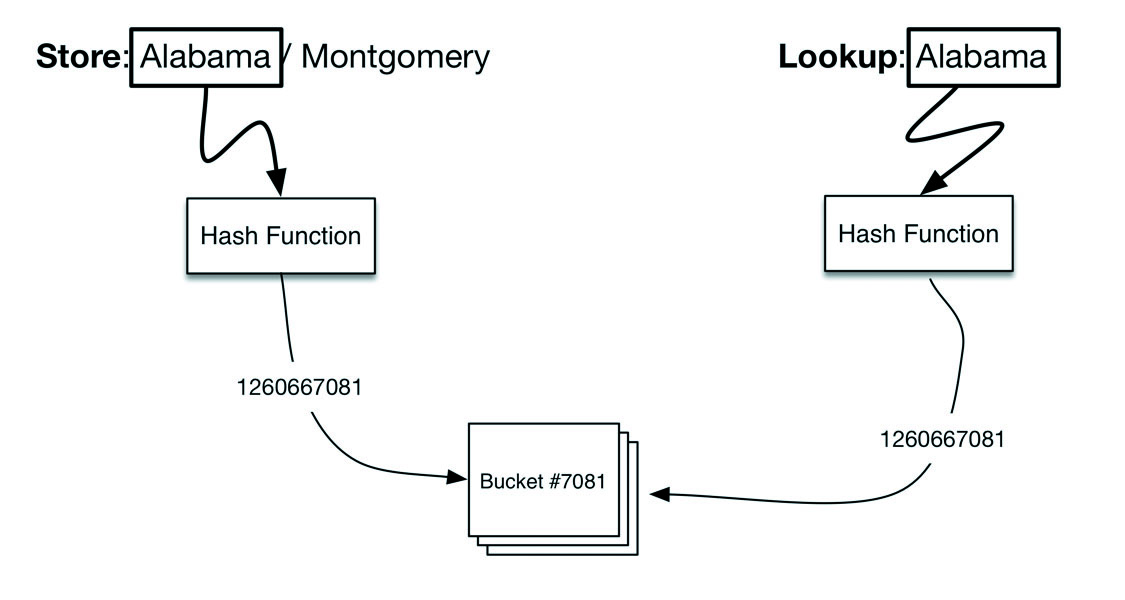
\includegraphics[scale=1]{images-cmyk/hash-table-process}
\end{center}
\caption{Hash table storage and retrieval.}
\label{fig:hash-table-process}
\end{figure}

\begin{figure}
\begin{center}
\begin{code}
\begin{verbatim}
(defun hash-op (hash-base chars)
   (if (consp chars)
       (+ (char-code (first chars))
          (* hash-base (hash-op hash-base (rest chars))))
       0))
(defun hash-key (hash-base wrd)
   (hash-op hash-base (coerce wrd 'list)))
(defun hash-idx (hash-base num-bkts wrd)
   (mod (hash-key hash-base wrd) num-bkts))
(defun rep (n x)
  (if (posp n)
      (cons x (rep (- n 1) x)) ; {rep1}
      nil))                    ; {rep0}
(defun bump-bkt (idx bkts)
   (if (posp idx)
       (cons (first bkts) (bump-bkt (- idx 1) (rest bkts)))
       (cons (+ 1 (first bkts)) (rest bkts))))
(defun fill-bkt-counts (hash-base num-bkts bkts wrds)
   (if (consp wrds)
       (let* ((idx (hash-idx hash-base num-bkts (first wrds)))
              (newbs (bump-bkt idx bkts)))
          (fill-bkt-counts hash-base num-bkts newbs (rest wrds)))
       bkts))
(defun hash-bucket-sizes (hash-base num-bkts wrds)
   (fill-bkt-counts hash-base num-bkts (rep num-bkts 0) wrds))
(defconst *example-tbl-25-most-common-English-words*
   (hash-bucket-sizes 31 10
      (list "the" "be" "to" "of" "and" "a" "in" "that" "have" "I"
            "it" "for" "not" "with" "he" "as" "you" "do" "at" "this"
            "but" "his" "by" "from" "they")))
\end{verbatim}
\end{code}
\caption{Prototype hashing operators (slow: using lists, not arrays).}
\label{fig:hash-defuns}\index{operator, by name!hash-op, hash-key, hash-idx}
\end{center}
\end{figure}

\begin{exercises}
\exer {Consider the words ``age,'' ``cage,'' and ``cape.''
Using the hash operator from this chapter, compute the hash key of each word
and the bucket the word maps to, assuming there are ten buckets.}

% NOTE: I took this exercise out because it's a very big project
%       and it calls for a lot of knowledge of ACL2 that we haven't
%       even hinted about, such as what form to use for input.
%       I guess it would be feasible (albeit a lot of busywork)
%       to do it with symbols and single quotes, but I don't want to
%       go into those issues in any detail. Too much ACL2 programming.
%\Exercise Implement the operator \textsf{state-idx} in ACL2. For this
%project, you will need to read about the built-in operators \textsf{char},
%\textsf{char-code}, and \textsf{coerce}
%in the online ACL2 documentation.
%Don't worry about whether 'A' is 1,
%'B' is 2, and so on. Any number will do, so just use the one that
%\textsf{char-code} delivers.

\exer {There are many websites on the internet that contain lists of words:
most popular baby names, most popular English words, and so on.\\
\hspace*{5mm}\url{https://www.babycenter.com/top-baby-names-2017.htm} \\
\hspace*{5mm}\url{https://www.englishclub.com/vocabulary/common-words-100.htm}\\
Pick a list of words and explore how the hash operator of this chapter works.
Use 31 for the hash base and try different sizes for the hash table.
In your project, try to answer the following questions:}
\subexer {How many search keys are there in the biggest bucket?}
\subexer {What is the average number of search keys in a bucket?}
\subexer {How many empty buckets are there?}
\subexer {What is the average length of a nonempty bucket?}
\subexer {Which one of these measures best estimates how well this hash works?}
\begin{quote}
You can use the operators defined in
figure~\ref{fig:hash-defuns} (page \pageref{fig:hash-defuns})
to get started on the project.
The operators use lists instead of arrays, so they are only  prototypes
for experimentation, not for practical use.
The definitions invoke some ACL2 intrinsic operators
that have not been discussed, such as
\textsf{coerce} and \textsf{char-code}.
The \textsf{coerce} operator converts a string to a list of characters,
and the \textsf{char-code} operator converts a character to a number.
The numbers are not the A 1, B 2, C 3, \dots, but that is immaterial.
Different characters are associated with different numbers,
which is the important thing. If you are interested,
you can find more information about these intrinsic
operators in the ACL2 online documentation.
\end{quote}
\end{exercises}

\section{Some Applications}

Hash tables provide an effective solution to the search problem,
so it is no surprise that they are all around us.
Hash tables are used behind the scenes in all sorts of applications.
They are ubiquitous.
Let's discuss some examples.

Hashing facilitates finding the definitions of operators
to run computer programs.
When you run a computer program,
the computer system needs to find the definitions
of the operators the program uses.
For example, the computer needs to know the definition of
\textsf{append} to compute the value of \textsf{(append [1 2] [3  4])}.
A lot of searches of this kind are required to run a program,
so a fast lookup procedure is important.

Hash tables offer a way to do it. Store the operator
definitions in a hash table where the key is the name of the operator
and the value is the definition. This is almost certainly the solution
that your computer system uses when it runs your ACL2 programs.
Another viable alternative is to use a binary search tree
(chapter \ref{ch:search-trees}), but hash tables work better
in this situation because there are a moderate number of search keys
(operator names), and they don't change very often.
With a binary search approach and, say, a few hundred keys,
a binary search would have five or ten computational steps,
while a good hash operator and corresponding hash table
might find operator names several times faster.

The number of steps in a binary search is proportional to the
logarithm of the number of keys. That's a lot less than the
number of keys, but it does grow slowly as the number of keys increases.
The amount of time it takes to perform a search using a hash table
is proportional to the number of keys in the biggest bucket.
Of course, the computation of the hash key and bucket index
also has to be factored in, but whether there are hundreds of search keys
or thousands, the time it takes to find a search
key stays about the same.

Database systems, the original killer app of
computing, are another common use of hashing.
Some of the earliest databases were used to keep track
of airline reservations, and now databases are used to store and
process all kinds of data: student records at a university,
transactions at every register in every Walmart,
cast members for every movie produced in Hollywood,
lifetime medical records for billions of people.
Organizations use databases to store literally
thousands of related records for each person involved in the system,
which can easily amount to billions
of records for an organization as a whole.

But what is a database system? At its core, a database system
manages one or more tables, and each table is made up of one or more
records consisting of several attributes.
Think of a database table as a
spreadsheet, where each record corresponds to a row in the spreadsheet
and each column corresponds to an attribute. If the table
records states and their capitals, each database
record (or row in the spreadsheet) would have one attribute for the
state name and another attribute for the capital.

It is common to design a database table in such a way that the
data in a particular attribute is sufficient
to single out a specific record in the database.
For example, a table containing student records might use the attribute
``Student ID'' to identify each student, so there would be
a column in the table containing student IDs.
Given a student ID, the
database system can find the record for that student in the
table. Part of the magic of database systems is that they can retrieve
records quickly using specialized data
structures called \emph{database indexes}.
Database systems use indexes to retrieve specific records quickly,
even when the table has millions of records that are stored
in separate files on disk drives.

So, what is a database index? Database systems
offer many different kinds of indexes, but there are two kinds that are
the most common. One is based on hashing, the other on trees.
In a sense, a database
table is a key/value pair, where the key is an attribute that is
sufficient to identify a particular record and the value is the record
it identifies.

Hash-based and tree-based indexes
in databases are,
in essence, hash tables similar to those in this chapter
and trees similar to those in chapter~\ref{ch:search-trees}.
The only substantial difference
is that our trees and hash tables are ACL2 objects that
reside in the fast-access memory of a computer,
whereas database indexes are designed to retrieve records
that can be stored in very large files.

However, database systems go beyond storing and retrieving records
using a key. They also excel at finding information by combining
records in different tables. For instance, one table may have
information regarding a student's permanent address and another table
may have information listing the students enrolled in any given course.
A database query can combine these tables to find the zip codes that
the students in any given course come from, perhaps showing that students in one
region of the country are more likely than those in another region to
enroll in history courses. That's the sort of insight that
data scientists find valuable.

Combining separate tables in a database can be expensive.
One way to proceed is to consider all possible pairs.
In the zip code example, you could look at each course
one at a time, and for each course consider
all the students who could be enrolled in it.
At a mid-sized university with 13,000 students
and 80,000 enrollment records, that would require
looking at over a billion combinations (1,040,000,000, actually).

Hash tables provide a simpler alternative. The student information table
and the course enrollment table are connected through the student ID.
So, before combining these tables, it is advantageous to hash both of them
using the student ID. Once this is done, each bucket contains some entries
from the student table and some from the course enrollment table. The entries
in each bucket must be considered exhaustively, but there is less work to do
than before.
To see this, suppose that there are 1,000 buckets,
each having an average of 13 students and 80 courses. Each bucket
contains $13 \times 80 =1{,}040$ combinations,
for a total of 1,040,000 combinations.
That makes retrieval a thousand times faster than the direct approach.

The reason that hash tables work so well in this context is that they take
a big problem and turn it into many smaller problems. Instead
of combining two tables of size 13,000 and 80,000, you can combine 1,000
tables of size 13 and 80. This savings is significant in itself, but it can
be even more dramatic if the smaller problems can be performed on different
computers. For example, if you have 1,000 computers, each one of them can be
working on a different bucket, so the total time to find the answer is
just the time to consider 1,040 combinations, which is a million times
faster than the direct approach.
This is the kind of thing that companies
with very large databases do---Google, Facebook, and Amazon, for example.
They use thousands of computers to process databases, and
hash tables are the key to spreading
the work evenly across the available computers.

Another important application of the hashing idea focuses on hash operators
rather than hash tables.
Suppose someone were to send you a very large file.
After waiting a few hours
for the file to transfer to your computer, how do you know that the file
you received is the same as the one that was sent?
It is possible that one of the characters
in the file was transmitted incorrectly because of a network glitch.
Or perhaps an intruder arranged to give you a false copy of the file.

Hash operators provide a way to address this problem.
Before sending the file, the sender could use a hash operator to compute a hash
value for the file. After you receive it, you would use the same hash operator
to create a hash key, and then you could compare the keys to make sure
they're identical. While it is \emph{possible} that two files end up with the
same hash key, a good hash operator makes it extremely unlikely.
Depending on how important it is, the hash operator can be designed to set
the bar at any level. The odds against
ending up with the same hash key, given two different files, can be
a thousand to one, or a million to one, or a billion to one.
The required level of security
determines what the odds against intrusion should be. Higher security
costs more, but the sensitivity of the information can justify the cost.
Variations of this idea are behind digital signatures and
also behind procedures for
keeping multiple copies of a file synchronized with one another.

Hash operators and hash tables are central to practical, large-scale computing.
We'll consider more aspects of large-scale, practical computing
in part IV of this book.

%%% Local Variables:
%%% mode: latex
%%% TeX-master: "book"
%%% End:


\part{Computation in Practice}

\chapter{Sharding with Facebook}

\index{Facebook}\index{social media}Facebook,
with billions of users and a profound, worldwide impact
on people, social interaction, commerce, and institutions,
is a major force far beyond its beginnings
as a way for college students to socialize online.
Having so many users poses tremendous technical challenges,
and Facebook's success is partly due to
the ability of its engineers to deal with these problems.
Many important technical innovations
have made the Facebook website possible.
Some of them are discussed in this chapter.

\section{The Technical Challenge}

To understand the challenges facing Facebook,
let's consider just one of its main features.
Facebook users can post frequent updates of their doings,
and they can view the postings of their friends through online connections
accessible from ubiquitous devices such as laptops, tablets, and cell phones.
Making this possible requires two lists of information for each user:
%\begin{quote}
%\begin{enumerate}
	%\item 
(1)~a list of the user's friends and
	%\item 
(2)~a list of the user's status updates.
%\end{enumerate}
%\end{quote}

It's not unusual for these lists to have hundreds of items,
so Facebook has to make hundreds of billions of items
accessible, quickly, online to billions of people.
That's this year. Next year, it may be trillions of items.

Traditionally, this data would be stored in a \index{database}database
using two tables, one for the status \index{update, database}updates
and one for the friends.  Figure~\ref{facebook-tables}
shows what these tables could look like.
Database software inserts, deletes, and modifies
rows on these tables as they evolve,
and supports sophisticated \index{query}queries that can
retrieve information from the tables.
For example, Facebook could use the following query to determine
what status updates to display when a specific user logs in:
\begin{code}
\begin{verbatim}
	SELECT   s.User, s.Time, s.Status
	FROM     Friends f, Statuses s
	WHERE    f.User='John'
	  AND    f.Friend = s.User
	ORDER BY s.Time DESC
\end{verbatim}
\end{code}

This approach would work very well if Facebook had a small number of users,
but it does not scale to billions users.
The problem is that a traditional database cannot process
this query quickly enough to keep up with a continuous
flood of online demand.

Facebook is not the only company that has this problem.
For example, \index{Amazon}\index{store front}Amazon
offers millions of items for sale.
It encourages customers to write reviews for each item, and it keeps a history
of purchases made by its customers so it can keep them informed about the status of orders,
make suggestions other purchases, and provide other services.
If the information were stored in traditional database tables,
retrieving it would take too long.

In fact, this is a problem faced by any
\index{Web 2.0 company}Web 2.0 organization.\footnote{A
Web 2.0 organization is one that allows large numbers
of users to produce content for its website.}
The web content that their users produce
can take the form of passages created directly by users,
such as Facebook updates or Amazon reviews, or it can be content created
indirectly, such as Amazon purchase recommendations.
When a Web 2.0 company is successful,
its users produce much more content than traditional databases can handle.

\begin{figure}
	\begin{center}
		\begin{tabular}[t]{ll}
			\hline
			\multicolumn{2}{c}{\textsc{Friends}} \\
			\hline
			\multicolumn{1}{c}{\textbf{User}} & \multicolumn{1}{c}{\textbf{Friend}} \\
			\hline
			John  & Sally \\
			John  & Mary \\
			Mary  & Sally \\
			Sally & David \\
			\hline
		\end{tabular}
		\hspace{.5in}
		\begin{tabular}[t]{llp{1in}}
			\hline
			\multicolumn{3}{c}{\textsc{Statuses}} \\
			\hline
			\multicolumn{1}{c}{\textbf{User}} & \multicolumn{1}{c}{\textbf{Time}} & \multicolumn{1}{c}{\textbf{Status}} \\
			\hline
			John  & Apr 21, 2011, 10:27 am & \raggedright Checked into Starbucks in Norman. \tabularnewline
			Sally & Apr 21, 2011, 10:29 am & \raggedright Saw \emph{Battle: Los Angeles} last night.  What a waste! \tabularnewline
			Mary  & Apr 21, 2011, 10:32 am & \raggedright Is anybody going to the carnival this weekend? \tabularnewline
			Sally & Apr 21, 2011, 10:33 am & \raggedright Looks like the fires are getting closer to our house.  Thinking about evacuating. \tabularnewline
			\hline
		\end{tabular}
	\end{center}
    \index{status update, database}\index{update, database}
	\caption{Tables for Facebook-style status updates.}
	\label{facebook-tables}
\end{figure}

\section{Stopgap Remedies}

\subsection{Caching}

Web 2.0 companies cannot use traditional databases
because, for example, it would take too long to retrieve information needed
to display a user's welcome screen.
One way to address this problem is to limit the number of queries that the
database needs to carry out.
For example, if many users check their home screens
several times in a span of a few minutes,
the computer can remember the results previous inquiries
instead of asking the database to
retrieve the home screen every time a user wants to check it.

That's called \emph{caching} the data.
A \index{cache}cache is a key/value store
in which data (values) are associated with keys
that facilitate locating the data,
like the search-tree keys of chapter \ref{ch:search-trees}
or the hash keys of chapter \ref{ch:hash-tables}.
When a query arrives, the database first checks
the cache to see if the information is already there.
If it is, it is simply reused.
Otherwise, the database performs the query against its underlying store,
and puts the results in the cache so they can be reused later.
A cache is much smaller than the underlying store
so data in the cache is frequently flushed and replaced with other active data.

Caching is useful when three conditions are met.
First, putting information in the cache and retrieving it
must be faster than ordinary database operations.
Much faster, so there is a significant gain
when the results are in the cache to make up for the delay when they're not.
Second, interactions with the database must frequently repeat the same transactions,
so that results stored in the cache are often reused.
Otherwise, caching data is a waste of time because it will
have been flushed from the cache before a second or third request arrives.
Third, \index{retrieval, database}retrieval
rather than update must be the dominant type of database transaction.
Updates can make the data in the cache inconsistent with information in the database,
forcing it to be retrieved again from the underlying store,
just as if there were no cache at all.
If it's not retrievals but updates that are the dominant transaction,
caching is a waste of time and effort.

Caching is used throughout the web.
It is especially successful in storefront applications,
where database queries often concern details about a particular product.
Storefronts offer hundreds of thousands of products,
but only a handful of them are really popular.
So, there are frequent requests for the same information,
which makes the cache effective.

Caching worked well for Amazon, at least before product reviews
and recommendations became prevalent in their product pages.
But caching cannot work well for Facebook.
Users look at their welcome pages on an individual basis,
and they make frequent postings. Retrieval of information
does not dominate the pattern of transactions,
and it is not the case that many incoming requests
are for retrieval of the same data, over and over,
the way it is with a storefront operation.
Besides that, one update on Facebook can trigger changes in many pages of the website.
This is typical in Web 2.0 applications,
and this need for frequent updates of customized information
for every user eliminates the advantages of caching.
Another solution is needed.

\subsection{Sharding}

\index{sharding}\emph{Sharding} splits a database into many different databases.
For example, John's Facebook friends and status updates may be stored in machine J, whereas
Mary's friends and status updates are stored in machine M.
Machines like J and M that store just a portion of the data are called \emph{shards}.
Because the database is stored on many different computers,
no one computer has to shoulder the entire load.
That's the upside.
The downside is that it makes it harder
to automate transactions with the database.
Programmers have to specify how to distribute
individual queries across all of the many computers
that may be involved in resolving the query.

To see how this might work,
suppose the computer needs to generate John's welcome page.
The first step might be to find John's friends,
which can be done by executing a query on machine J.
\begin{code}
\begin{verbatim}
	SELECT   f.Friend
	FROM     Friends f
	WHERE    f.user='John'
\end{verbatim}
\end{code}

The query returns John's friends, Sally and Mary.
The next step is to find Sally's and Mary's status updates.
That leads to the the following queries:
\begin{code}
\begin{verbatim}
	SELECT   s.Time, s.Status
	FROM     Statuses s
	WHERE    s.User='Sally'
	ORDER BY s.Time DESC

	SELECT   s.Time, s.Status
	FROM     Statuses s
	WHERE    s.User='Mary'
	ORDER BY s.Time DESC
\end{verbatim}
\end{code}

The first query should run on machine S,
whereas the second query should run on machine M.
The final step is to combine the results from the two queries
and then merge them, keeping
the combined list in reverse chronological order.

Queries like this show one of the shortcomings of sharding.
Each query retrieves results from only one table
because the related \index{record, database}records
are not necessarily stored in the same shard.
In this particular example, the information needed to answer the query was
distributed across shards J, S, and M.
So the program had to collect the information
from all the different sources and then combine it.
Clearly, using sharding is more complicated
than keeping all the information in one place,
as in a traditional database.

Sharding also suffers from uneven distribution.
What if, for example, one of the shards ends up with too many records?
That shard would need to be split into pieces.
For example, the system could
split the shard M into two shards, Ma-Mp and Mq-Mz.
That seems like a good idea, but in practice splitting shards
is complicated because the software on all the computers that access the data
needs to be modified to make it possible for the computers
to find the shard that contains the information they're looking for.

\section{The Cassandra Solution}

Faced with these difficulties, Facebook engineers developed a solution that
retained the benefits of sharding, but avoided some of the difficulties.
The goal was to make it easy to split a shard into multiple pieces
and to hide from the software the complexity of sharding.

\index{Cassandra}Cassandra, the solution they devised, combines features
from the Dynamo project at Amazon and the BigTable project at Google.
From Dynamo, Cassandra borrows the idea of a replication ring,
and from BigTable, a data model.
Cassandra's data model groups records into different tables.
Each record in a table is identified with a key.
The key must be unique in a given table,
but the same key may be used in different tables.
Each record consists of one or more key/value pairs, and
different records in a Cassandra table may have different keys.

For example, John's friends may be stored in a record like the one shown in figure~\ref{users-table}.
The important thing is that a program can retrieve
all of John's friends by requesting the single record with ID John.
Once John's friends are known, it is necessary to retrieve their status updates.
This can be done by looking for the records in the status table that have the appropriate record IDs.
Figure~\ref{status-table} shows what the status table could look like.

The table structures we have presented assume that all fields will fit in a single record.
That is, we assume that a single record can hold all of a user's friends or all of a user's status updates.
Cassandra tables are designed to support thousands of fields.
This will be enough for most users, but not for the heaviest users of Facebook.
To deal with the heaviest users, Facebook can reuse the same idea with column names.
To support an arbitrary number of friends or status updates,
the values can be spread across multiple records, 
with IDs such as John1, John2, and so on.

\begin{figure}
	\begin{center}
		\begin{tabular}[t]{lll}
			\hline
			\multicolumn{3}{c}{\textsc{Friends}} \\
			\hline
			\multicolumn{1}{c}{\textbf{Record ID}} & \multicolumn{1}{c}{\textbf{Friend1}} & \multicolumn{1}{c}{\textbf{Friend2}} \\
			\hline
			John  & Sally & Mary \\
			Mary  & Sally & \\
			Sally & David & \\
			\hline
		\end{tabular}
	\end{center}
	\caption{Storing friends lists in Cassandra.}
	\label{users-table}
\end{figure}

\begin{figure}
	\begin{center}
		\begin{tabular}[t]{lp{.8in}p{.8in}p{1in}p{1in}}
			\hline
			\multicolumn{5}{c}{\textsc{Statuses}} \\
			\hline
			\multicolumn{1}{c}{\textbf{Record ID}} & \multicolumn{1}{c}{\textbf{Time1}} & \multicolumn{1}{c}{\textbf{Time2}}
				& \multicolumn{1}{c}{\textbf{Status1}} & \multicolumn{1}{c}{\textbf{Status2}} \\
			\hline
			Sally & \raggedright Apr 21, 2011,\hfill\break10:29 am & \raggedright Apr 21, 2011,\hfill\break10:33 am &
				\raggedright Saw \emph{Battle: Los Angeles} last night.  What a waste! &
				\raggedright Looks like the fires are getting closer to our house.  Thinking about evacuating. \tabularnewline
			\hline
		\end{tabular}
	\end{center}
	\caption{Storing status updates in Cassandra.}
	\label{status-table}
\end{figure}

The upshot is that the workflow for retrieving information from Cassandra
is similar to the workflow for sharding but with a major difference.
The queries that are generated do not need to be aware
of which shard contains the information they need.
In fact, Cassandra relies on sharding both for performance and for replication.
The key innovation is that the shards are arranged in a ring.
For simplicity, assume that the shards are labeled A, B, C, \dots, Z.
The ring arrangement means that each shard is connected to the next,
and eventually the last shard is connected to the first.
For example, A could be connected to B, B to C, and so on, until Z is connected back to A.

Records are arranged in an order determined by a hash function
that computes a hash value from the key of a record.
The hash value is used select a shard label (labels A through Z in the example).
All hash values up to A are mapped to shard B,
those between A and B to shard C, and so on.
The hash function and mapping of hash values to shards is known to every shard,
so a program can ask any of the machines to retrieve a given value.
If the machine does not have the value,
it can determine the shard containing the value
and forward the request to that shard.

The ring makes it easier to rebalance the shards
in case one of them becomes too large.
Suppose, for example, shard B gets too large.
To balance it, a new shard, say BM, is created and inserted between B and C.
During the insertion process, B sends all of its records between BM and C to shard BM.
%\todo{Question (11/22/17):
%      Earlier it said that all hash values between B and C mapped to C.
%      Now, it says that records between BM and C are sent to shard BM.
%      It's not clear to me what that means. If "record between BM and C"
%      means hash values between BM and C, then it seems that the record
%      should be sent to shard C, based on the earlier specification.
%      If "record between BM and C" means something other than hash value,
%      then something needs to be said about what it means.
%      Also, it's not clear whether shard and machine mean the same thing
%      or if they are different things. From what is said, they its seems
%      that machine and shard mean the same thing.
%      This needs clarification.}
When this process completes, all shards are notified of the new
shard's existence and shard BM joins the ring.
This can happen without the knowledge of any programs
that are retrieving data from the system.

Cassandra also uses the ring for \index{replication, database}replication.
Records that should be stored in A
are also stored in B and C.
This is important, because computers and disks can fail,
but if shard A should fail, there are two more copies of its data.
It can also serve to improve performance during spikes.
If shard A becomes busy, shards B and C can take over some of the load.

Replication complicates the splitting of shards.
When shard B is split into B and BM, for example, this also affects shards C and D
because they store replicated records for shard B.
Now this needs to be restructured, so that B's records are replicated in shards BM and C.
Moreover, C and D should replicate the records for shard BM.
This means that shards C and D need
to participate in the insertion of BM into the ring.
Shard C needs to know that some of the records
it replicated for B are now associated with BM instead.
Shard D needs to know that some of the records it was replicating
on behalf of B can now be forgotten, and the rest need to be associated with BM.
Finally, the new shard BM needs to receive not just its share
of B's records but all of B's records so that it can replicate B's remaining data.

That's a lot of data movement, and it might be surprising that it helps.
Part of the reason it works is that Facebook has the luxury of not having
to get all the data right all the time.
If people don't see all the latest postings of their friends until
an hour or even several hours after they are posted, it's no big deal.
Users may be a little out of synch for awhile, but the data is not time critical
on a minute-by-minute basis.

\section{Summary}

Web 2.0 applications bring up many scaling challenges.
These challenges go beyond what traditional database solutions can offer.
So, leading Web 2.0 companies have developed custom solutions,
and the idea of sharding plays a prominent role in some of those solutions.
Cassandra, Facebook's solution, successfully met the challenge, and
fortunately, Facebook decided to make \index{Cassandra}Cassandra available to the
programming community via an open-source process.

Programmers can download Cassandra (\url{http://cassandra.apache.org})
and use it to develop new software.

%%% Local Variables:
%%% mode: latex
%%% TeX-master: "book"
%%% End:


\chapter{Parallel Computation with MapReduce}

\section{Vertical and Horizontal Scaling}

Some important computer applications are so large that they would take
unacceptably long to run on conventional computers.  For
example, a personal computer is more than powerful enough
to balance your checkbook but not for a financial
application that tracks credit card usage in real time to
detect instances of fraud.  The sheer number of credit card
transactions make this application far too intense for a
personal computer.

There are various ways to cope
with problems of scale  in large applications.
The traditional approach is
\index{scaling!vertical}\index{vertical scaling}\emph{vertical scaling},
which means running the
application on a more powerful computer.
This is the easiest solution in terms of software
because the software does not need to change as the machine scales up.
But what happens when the problem gets bigger than any single machine can handle?
For example, maybe a big, fast computer could handle
a billion credit card transactions an hour
but not a hundred billion.
At some point, the rate at which transactions take place
will overwhelm the available computing technology.

\index{scaling!horizontal}\index{horizontal scaling}\emph{Horizontal scaling}
offers an alternative.  Instead of
running the application on a single computer,
the application is split into smaller
chunks, and each chunk is run on a separate computer.
Ideally, all of the computers involved are similar in most respects
to personal computers, so that the cost of an additional
machine is a small fraction of the overall system cost.
This makes it economically feasible to scale the
hardware platform as the computation requirements increase.
Horizontal scaling has become the de facto
solution for dealing with web services that have to deal
with rapid growth, such as those provided by
Facebook, Google, eBay, Amazon, Netflix, and many others.

The problem with horizontal scaling, however, is that it is
not always easy to split an application into smaller
chunks.  In fact, this is particularly hard when the program
is written using conventional programming languages, such as
C++ or Java. In conventional languages, the program specifies
a sequence of updates to records stored mostly in fast memory.
That makes it difficult to manage multiple computers
working on the computation at the same time because the
cooperating computers need to coordinate their updates.
The coordination problem can sink the effort to make
the computation go faster.
Getting the appropriate data and the right software
components to the right computer
at the right time presents a host of problems.

One advantage of an equation-based software model
is that the different parts of the software are more decoupled
than they are with the conventional approach.
Everything is defined in terms of operators
that, given operands with appropriate data,
can produce results without
interacting with other parts of the software.
For that reason, it does not matter where or when
the operations are performed.
The problems of getting the right data to the right place
remains, but the task of managing a great many small interactions
between different parts of the software is greatly reduced.

The engineers at Google were faced with one of the largest
scaling problems that computing had ever seen,
namely, searching the entire, rapidly growing, worldwide web.
To cope with the scale of this problem and its continual growth,
the horizontal scaling approach was the only practical option.
Even though they use mostly conventional programming methods
for most of their software,
they invented and adopted a way to manage large-scale components
with a programming model called \index{MapReduce}MapReduce
that has a lot in common equation-based software models.
Since Google's introduction of MapReduce,
it has been adopted in many other settings.  For
instance, the \index{Apache Foundation}Apache Foundation
implemented \index{Hadoop}Hadoop, an
open-source implementation of MapReduce that you can
download for free to your computer.
Hadoop is widely used in commercial applications and in research.
We will describe the general nature of
MapReduce systems like Hadoop
and explain how the MapReduce framework simplifies the
development of programs that can scale horizontally by
focusing on just two operations: Map and \index{reduce, map}Reduce.

\section{The MapReduce Strategy}

The \index{reduce, map}\index{MapReduce}\textsf{MapReduce} paradigm
is applicable to problems that process
data that can be represented as a sequence of
\index{key/value pair}key/value pairs.
Not all problems lend themselves to this representation,
but Google engineers recognized that many practical
problems do fit in this category.
The following are a few examples:

\begin{quote}
\begin{itemize}
\item \emph{Counting Words in a Document.}  The data in this
case is the collection of words in a document.  It can be
organized as a list of word/count pairs, where the counts
are initially set to one.  Since any word may appear
multiple times in the document, most words will, in the beginning,
occur in more than one word/count pair.
The objective is to produce a list of word/count pairs
in which each word appears only once and the associated
count is the number of occurrences of
the word in the document.

\item \emph{Finding Words that Link to a Webpage.}  The
purpose of this operation is to find the words that are
most commonly used to link to a particular \index{URL}URL.
For example, your name may be the most
common phrase used to link into your Facebook page.
Google uses this kind of information to select which
pages to display for a particular search.
The MapReduce approach applies to this problem.
The data is the
collection of links on the Internet.\footnote{Nobody knows how many
links there are on the internet, worldwide,
but most estimates place it in the trillions,
and some credible estimates place it in the hundreds of trillions. }
Each link can be represented as a word/URL pair,
where the same word may appear in many different pairs.
To figure out which words are most commonly associated with
a particular web address,
this data needs to be reduced to a collection of
URL/word pairs, where each URL will appear once, associated
with the word that is used most often to link to that URL.

\item \emph{Finding Extreme Values.}  Consider
an application that finds the record high or low temperature
for each of the fifty states of the U.S.
The initial data consists of a list of
city/temperature pairs.  There would be one record for each
recorded temperature in a city. It might be one per day,
one per hour, one per minute, or a varying combination,
depending on the city, and the records would extend over
different periods of time for different cities,
a hundred years for some cities, ten years for others,
and so on. So, each city would occur in many different pairs.
The desired outcome is a collection of city/temperature
pairs where each city occurs only once, and the associated
temperature is the highest (or lowest) one in the recorded data.
\end{itemize}
\end{quote}

What all these applications have in common is that data processing
can be split into three different parts, each involving a list of
key/value pairs, and it is possible to process each individual
data record or key/value pair without having to simultaneously
examine all the other records.  For
example, consider the case of finding the highest
temperature ever recorded in each of the fifty states.
The computation could proceed in three stages:
\begin{quote}
\begin{enumerate}
    \item \textbf{Input Data} pairs temperatures with associated sensors.
        Each pair could have a key identifying a
        specific temperature sensor and
        a value that consists of the city and state where
        the sensor was located, the date the sensor measured
        the temperature, and the temperature on that date.
        For example, the input data may contain the following
        records:
        \begin {quote}
        \begin{itemize}
            \item \textsf{KLAR, Laramie, WY, 2009-05-13, 41}
            \item \textsf{KLAR, Laramie, WY, 2009-05-14, 47}
            \item \textsf{KOUN, Norman,  OK, 2009-05-13, 76}
            \item \textsf{KOUN, Norman,  OK, 2009-05-14, 70}
        \end{itemize}
        \hspace*{1cm}$\vdots$
        \end{quote}
        The first column is the key for each record (for example, KLAR),
        and the remaining columns comprise the value. Many
        records may have the same key in the input data because the
        sensor makes many measurements over time.
        The goal is to reduce that to records
        in which each key appears only once,
        associated with the maximum temperature measured by that sensor.
    \item \textbf{Intermediate Data} is used to pass data from
        the Map operation to the Reduce operation. The Map operation
        processes the \emph{input data} and produces key/value pairs
        that make up the \emph{intermediate data}, and the Reduce operation
        processes the intermediate data to create \emph{output data}.
        In this application, the goal is to find the highest temperature
        for each state, so the Map operation could extract
        the state and temperature from each input data record.
        Then, the intermediate records would be state/temperature pairs.
        \begin {quote}
        \begin{itemize}
            \item \textsf{WY, 41}
            \item \textsf{WY, 47}
            \item \textsf{OK, 76}
            \item \textsf{OK, 70}
        \end{itemize}
        \hspace*{1cm}$\vdots$
        \end{quote}
        In general, the Map operation may produce any number of intermediate
        data points for any given input data record, although in this case,
        precisely one intermediate record is generated for each input record.
    \item \textbf{Output Data}, the final result of the MapReduce computation,
        is delivered by the Reduce operation.
        In the high-temperature example, this
        corresponds to the maximum temperature recorded for each state, so
        there would be exactly one record for each state that appeared in the input data.
        \begin {quote}
        \begin{itemize}
            \item \textsf{WY, 115}
            \item \textsf{OK, 120}
        \end{itemize}
        \hspace*{1cm}$\vdots$
        \end{quote}
\end{enumerate}
\end{quote}
As you can see, the data records are largely independent of one another, so the computer
can process the May 13, 2009 temperature entry for Norman, OK, without considering the
May 13, 2009 entry for Laramie, WY.  This enables horizontal scaling because the
different entries can be processed in different machines.
However, this application also shows the need for combining
the entries for a specific key at a later time.  For example,
to find the high-temperature record for Oklahoma, it will be
necessary to consider all the entries for Oklahoma at some
point.

The MapReduce paradigm applies well in these kinds of problems.
The \textsf{map} operation, which receives each
of the input key/value pairs, processes the
pair and produces a large number of intermediate
key/value pairs.  These intermediate pairs use keys that may
or may not be completely different than the input keys.
In the word-counting example, the intermediate keys may be the same
as the input keys, namely, the words that are being counted.
On the other hand, when looking for words that are used to
link to URLs, the input keys are the words, but the
intermediate keys are the URLs. The MapReduce framework leaves
this choice up to the software designer, which is
one of the reasons that MapReduce is widely applicable.

The second step is the \index{reduce, map}\textsf{reduce}
operation, which combines all the entries
for the intermediate keys and
produces zero or more output key/value pairs.  As before, the
output key/value pairs may use the same keys as the
intermediate or input key/value pairs, or they may use
entirely different keys.

For example, consider the problem of counting words in a
document.  Assume that the document has already been
read and that it has been broken up into key/value pairs,
where each key is a word and the value is always one. These
key/value pairs make up the input data for this problem. For
instance, the Gettysburg address could be represented by a
list of key/value pairs using the notation ( \emph{key} ~.~ \emph{value} )
to denote a pair.
\begin{quote}
\begin{itemize}
\item \textsf{( four~.~1 )}
\item \textsf{( score~.~1 )}
\item \textsf{( and~.~1 )}
\item \textsf{( seven~.~1 )}
\item \textsf{( years~.~1 )}\\~~~~$\vdots$
\item \textsf{( from~.~1 )}
\item \textsf{( the~.~1 )}
\item \textsf{( earth~.~1 )}
\end{itemize}
\end{quote}

The \textsf{map} operation takes in an input key and
value and delivers a list of zero or more intermediate
key/value pairs.  For the word-count program, map could
deliver a list with exactly one element, namely,
the very same input key and value.
In this case, the map part of MapReduce
packages the result in a list, which is
the form expected by the MapReduce system,
but does not perform any additional computation.
\begin{displaymath}
map(k, v) = [ ( k ~.~ v ) ]
\end{displaymath}
In a more elaborate example, map would perform
a computation using the key/value pair supplied as
its operand and deliver a list representing the results
of that computation.

The \textsf{reduce} operation accepts an intermediate key and a list of
all the values returned by any map operation for that key.
It delivers a list of zero or more final key/value pairs.
In the case of word count, reduce returns only one key/value pair,
namely, the key and the sum of the counts in the list.
\begin{displaymath}
reduce(k, vs) = [ ( k ~.~ sumlist(vs) ) ]
\end{displaymath}
The operator \textsf{sumlist}, which adds all the elements of its
input, would be defined by the software designer.

To make this discussion more concrete, consider the Gettysburg Address,
which contains the word ``nation'' in four places. Because of this,
the map operation will be called with the input key/value pair \textsf{(nation~.~1)}
four times, and each time it will return a list with
the single intermediate key/value pair \textsf{[(nation~.~1)]}. The MapReduce
system collects all the values for each intermediate key and starts the reduce
operation on those values.
At some point, it will collect all of the four intermediate
values for ``nation'' and invoke the reduce operation with the operands
\textsf{nation} and \textsf{[1 1 1 1]}.
The reduce operation will then
return a list with the final key/value pair \textsf{[(nation~.~4)]}.

% \todo{QUESTION (11/23/17): I don't think this makes sense.
%      Where does vs come from? Earlier, map produced [(k~.~v)].
%      There was no list of vs, just one v. It seems that
%      reduce could create the vs list, but map couldn't supply it
%      a list of vs for each k, but not a list of all the v's
%      associated with a particular k-value. The reduce step
%      could coalesce the duplicate k-values, but that's
%      it wouldn't help much to have reduce sum the v's for
%      non-coalesced k-values.
%      Maybe it would be better to define
%      map(k, v) = v, then explain that the MapReduce
%      system forms a list of all the results produced
%      by map when it operates on the key/value pairs, one by one,
%      then talk about what the reduce step does in this example.
%      Or something.}

Much of the value of MapReduce is that the programmer only needs to
define the map and reduce operations and
does not need to deal with the details of carrying out the map and reduce
operations in a collection of computers sharing the data across a
network.  It is the MapReduce
framework that takes care of running the program in a single
computer or in a cluster of hundreds or even hundreds of thousands
of computers, depending on the size of the problem.
It also takes care of things like
sending the intermediate key/value pairs
from the computers processing the map operation to the computers
processing the reduce operation.

The MapReduce framework
takes the input key/value pairs and splits them across many
different machines.  On each machine, it performs the map
operation on each of the key/value pairs that is assigned to
that machine.  As it does this, it combines the intermediate
key/value pairs returned by each map operation into a single
list.  The lists from all of the machines are then combined.

The intermediate lists must be combined because
the reduce operation expects to see an intermediate key and all
of the values associated with that key at the same time. For example,
to find the maximum temperature for the key \textsf{OK}, the reduce
task needs to see all the records associated with \textsf{OK}.
Different intermediate keys, such as the ones for \textsf{OK} and \textsf{WY},
are independent, so they can be processed by different machines.
That is, one machine can process \textsf{OK} temperatures at the same
time that another machine is processing \textsf{WY}.
But all of the \textsf{OK} records must go to the same machine running
the reduce operation for \textsf{OK}.
Therefore, the map operation collects all of the values for
each of the intermediate keys, and then the reduce operation is
called only once for each intermediate key.

Once all the values for a given intermediate key are
collected, the MapReduce framework can call the reduce
operation on that intermediate key.  The result is a list of
output key/value pairs. MapReduce collects all these
results and returns them as the final result of the computation.

MapReduce does the work of distributing
the program across multiple machines.
That is one way it provides value.
An engineer can develop a MapReduce program on
a local computer and modify it until it behaves as
required on a small data set.
Then, the program can be submitted to a large MapReduce cluster
to process a full-scale data set.
The MapReduce system deals with the problem of scale
automatically once the program has been developed.

\section{Data Mining with MapReduce}

\index{data mining}\index{mining, data}Now
that we have seen the basics of MapReduce, we can look at
a larger example that illustrates how MapReduce is
used in practice.  The application we will discuss is a recommendation engine,
a piece of code that is used to recommend new things to a person
based on other things the person likes.
For example, the product page that pops up on a typical visit to
the Amazon website often has a section called ``Customers Who Bought
This Item Also Bought'' that recommends related items.
Based on past purchases and browsing habits, the Amazon software
builds a customized web page full of recommendations.
How does Amazon do this?

Let's break the problem down into
two components.  First, \index{Amazon}Amazon
needs to find \emph{customers like you}.
In the case of a single product, this means other customers who
have bought that product.  In the more general sense,
it means other customers who have bought many
of the same items that you have purchased in the past.
Once the group of
customers like you is identified, the purchases
that people in the group have made can be examined
to find the most popular items.

Finding the most popular items is a problem that is a lot like
counting words in a document.
Amazon keeps a history of all the purchases that each
customer has made.  To process this list with MapReduce, think of it as
consisting of entries of the form customer/item, meaning that at some time the specified
customer bought that particular item.
The map operation produces intermediate entries of the type item/1, meaning
the given item was bought (once),
which is similar to what the word-count program did.
Such an entry should be generated for
each purchase made by a customer in the reference group.  That is,
the map operation filters out the purchases made by customers who are
not like you. The reduce operation is identical to that of word-count,
but this time it counts the number of purchases for each item.
In the end, the computation must consider the results of the reduce operation
and select the items that were purchased most often.

Unfortunately, that leaves the first problem unsolved: finding the group of
customers who are most like you.  This is the most critical aspect for
generating useful recommendations.  For instance, if all of your purchases
from Amazon have been gardening books, you are likely to ignore a
recommendation engine that alerts you to the latest novel in a long-running
vampire series.  Worse, you may start thinking of the recommendations
as unwarranted spam.

How can Amazon find other customers like you?  Imagine that
you have rated all the purchases you have made, giving each item a grade between
0 (hated it) and 5 (loved it).  To keep things simple, imagine that Amazon
sells only two items.  Then your ratings for these items can be expressed as
a pair of numbers, say (2, 0).  Now suppose that other customers have also
rated the items.  The customers who are most like you are the ones
whose ratings are close to yours.
One way to measure how close other ratings are to the pair (2, 0)
is to view the pair
as the coordinates of a point in a two-dimensional plane.
Using this notion of closeness, the customers who
are most like you have purchase histories that correspond to nearby
points in that plane.\footnote{To
determine what points are ``nearby,'' you will need
some notion of distance in the plane. You could use the standard
Euclidean distance or some other distance measurement customized
to the problem of solving the customers-like-you problem.
This is just one of the complex issues that come up
in fashioning methods for finding clusters in data.}

Of course, Amazon sells many more than two items, and neither you nor any
of Amazon's other customers are likely to have rated even a fraction of them.
But the principle stays the same.  Instead of using pairs to represent
ratings, many more coordinates would be needed, as many coordinates
as the number of different products Amazon sells.
The coordinates would still specify a point in space,
but it would be a space with many dimensions.
The customers most like you will still be represented by points close to yours
in that multidimensional space.

A remaining complication is that customers do not always explicitly rate the
items they like, but this can be resolved by using implicit ratings.
For example, if you buy an item, we can give it a rating of 4 unless you
explicitly change it.  And any product that you have never looked at
can be given a rating of 0.

The problem is to find which points in this huge domain with many dimensions
are near your own. Or, viewed another way, the problem is to find groups of
points that are clustered together. One cluster, for example, may consist of
avid gardeners, whereas another is made up of fans of vampiric fiction.

In general, finding \index{clusters, finding}clusters
in a large data set is a difficult problem
that has been studied extensively
by scientists and mathematicians for a long time.
There are many useful approaches.  One that, on the surface at least,
is straightforward to describe starts with guessing some cluster locations,
then gradually refining the guesses by making computations based on the data.
The computation could proceed as follows:
\begin{quote}
\label{cluster-process}
\begin{enumerate}
    \item Initially, guess a location for each cluster. The guess can be
        taken as the estimated center point of each alleged cluster.
    \item For each point in the data set, decide which cluster center is nearest
        to the point.  Split the points into clusters so that each point is
        in the cluster determined by the nearest center point.
    \item Recalculate each cluster's center point by averaging all the
        points that were assigned to that cluster.
    \item Repeat the previous two steps until things settle down or meet
        some other predetermined conditions.
\end{enumerate}
\end{quote}
The middle two steps can be implemented using MapReduce.  The map operation can
assign points to clusters, and the reduce operation can compute the new center
point of each cluster.  The distances between data points
and estimated cluster centers determines which cluster the data point belongs to,
and the cluster determines the products of interest to particular customers.

The map and reduce operations defined by the programmer
must conform to the expectations of the MapReduce framework.
The framework requires the map operation to be based on
key/value pairs.  In this application, the job of map is
to figure out, for each customer, which cluster center
is closest to that customer's purchase history.
This must be done for all customers, but the MapReduce
framework will take care of distributing the operation across all customers.
We just have to say what the map operation does for an individual customer.

Let's say that the purchase history for the customer is the first operand
of the map operation and the list of cluster centers is the second operand.
Using this information, the map operation selects the center that is closest
to the customer's purchase history. The MapReduce framework requires the map
operation to deliver its result in the form of a list of key/value pairs,
and we can meet this requirement by specifying that the map operation
delivers a list of just one element, which is a pair consisting of
the selected center (the key) and the purchase history (the value).
\begin{displaymath}
map(hist, centers) = [ ( closest\_center(hist, centers) ~.~ hist ) ]
\end{displaymath}

% \todo{QUESTION (11/23/17): But what is the purpose of v?
%       The result does not seem to depend on it. Is this some kind of
%       symmetry thing, like the symmetry for reduce, below?
%       Needs some kind of explanation.}
The MapReduce framework applies the map operation to all the customers,
gathers up the results, and packages them in the form of
intermediate key/value pairs, one for each cluster center (the key).
The value that the framework associates with the key is the list of
points in the purchase histories associated with the cluster center that
the key represents.
In the equation that defines the map operation,
the center delivered as the key is computed by an operator
called $closest\_center$, which does the work of selecting one
of the centers from the list supplied as its second operand.
The one it selects is, of course, the one that is closest to
the customer history supplied as its first operand.

The $closest\_center$ operation would need to be defined,
and the details depend on how distances between
points are measured. We have deferred deciding those
details, so we will leave that part of the computation
out of the discussion.
In any case, an intermediate key/value pair is a cluster center
(the key) and a list of nearby purchase histories
(the value). Each purchase history is a point for which the
key is the nearest cluster center to that point.
The MapReduce framework sends the intermediate key/value pairs
to the reduce stage of the process.
Now we need to turn our attention to the reduce operation.

The reduce operation receives
an intermediate key/value pair from the MapReduce framework.
The key is the center of a cluster, which is treated by the reduce operation
as an identifier for the cluster.
The value is a list of the points in the cluster.
The job of the reduce operation is to compute a new
center for the cluster (the key) by averaging the list of points (the value).
The MapReduce framework requires the reduce operation to deliver
a list of key/value pairs, so we package its result as a list consisting
of exactly one key/value pair, namely, the cluster identifier (the key) and the
new center (the value).
\begin{spacing}{0.9}
\begin{eqnarray*}
    \begin{array}{l@{}l}
        reduce(&cluster, \\
               &points)
    \end{array} &=& [ ( cluster ~.~ average(points) ) ] \\
average(points) &=& avg(points, (0,0), 0) \\
\begin{array}{l@{}l}
    avg(&points, \\
        &sum, \\
        &count)
\end{array} &=&
    \left\{
        \begin{array}{l@{}ll}
            \multicolumn{2}{l}{sum / count} & \mbox{if } points = [~] \\
            avg(& rest(points),             & \mbox{otherwise} \\
                & sum+first(points),        & \\
                & count+1)                  & \\
        \end{array}
    \right.
\end{eqnarray*}
\end{spacing}

We need to explain some of the operators and terms
in the equations that define the reduce operation
because they are not, in all cases, what might be expected.
The \emph{points} variable refers to a list of points,
and each point is a pair of numbers representing product ratings
by a customer.
The operand $(0,0)$ in the equation that defines $average$ is
also a pair of numbers, both zeros in this case.
These zeros serve as a starting point for adding
up the product ratings to make it possible to compute
averages.\footnote{There are only two product ratings
to simplify the example. In practice, there would be
many product ratings, so the data item representing
a customer's ratings (and the initial item with the
zeros that start the calculation)
would have many components, each processed in a manner analogous
to the two-component ratings in the example.}

The $sum$ variable is also a pair of numbers.
Therefore, the addition ($+$) and division ($/$) operators
with $sum$ as a left-hand operand are not the usual arithmetic operators.
The formula $sum + point$ denotes $(s_1, s_2) + (r_1,r_2)$,
which stands for the pair $(s_1+r_1, s_2+r_2)$.
Similarly, $sum/count$ denotes $(s_1,s_2)/count$,
which stands for $(s_1/count, s_2/count)$.
The definitions also refer to the operators $first$ and $rest$.
The operator $first$ delivers the first point in the list of points,
and the operator $rest$ delivers all the points in the list
after the first one.

Finally, the equation defining $avg$ selects one of two formulas,
depending on the value of $points$, which is a list.
If the list is empty (that is, if $points = [~]$),
the formula $sum/count$ is selected as the value of $avg$.
If $points$ is not the empty list, the definition selects
a more complicated formula as the value of $avg$.

There is an important subtlety in the way the equations define
the operator $average$ that computes a new center point of a cluster
from points assigned to that cluster in the map stage of the
MapReduce computation.
The work of computing the average is done by the $avg$ operator.
The definition of $avg$ is inductive and
employs a common trick known as tail recursion
that makes computations like averaging much faster.
We think it is worth complicating the discussion
with this technique because the main point
of MapReduce is to be able to compute things quickly.
The \index{tail recursion}\index{recursive}tail recursion
trick avoids supplying, as an operand to another operator,
the value that $avg$ delivers.
This makes the computation
faster because the computer is able to avoid a lot of bookkeeping
that is required when an inductive
invocation is nested in an invocation of another
operator.\footnote{Section \ref{sec:lemmas} discusses an
example illustrating the effectiveness of tail recursion.}

The result of the reduce operation is a new list of center points
in the same format as the initial guess.
That makes the output of the
reduce operation suitable as
the initial guess for additional map computation steps,
which makes it possible for the computer to perform as many
map/reduce cycles as necessary to find clusters.
Figure~\ref{iterative-map-reduce} (page \pageref{iterative-map-reduce})
diagrams the MapReduce
process that we applied to implement the four-part clustering procedure
discussed earlier (page \pageref{cluster-process}).

\begin{figure}
    \begin{center}
%        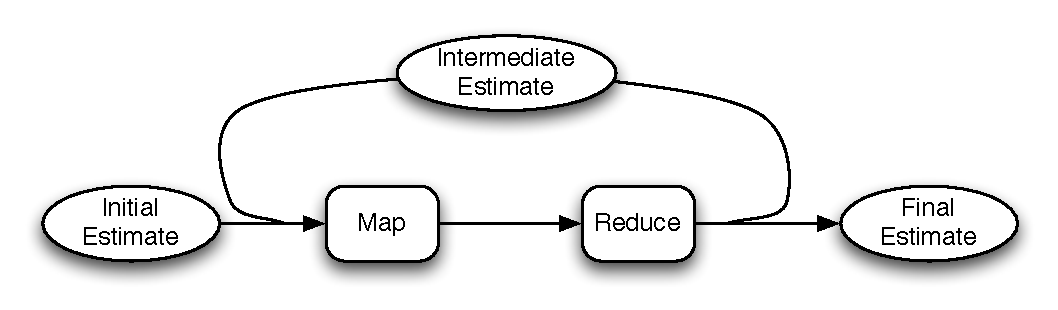
\includegraphics[scale=0.7]{images/iterative-map-reduce}
        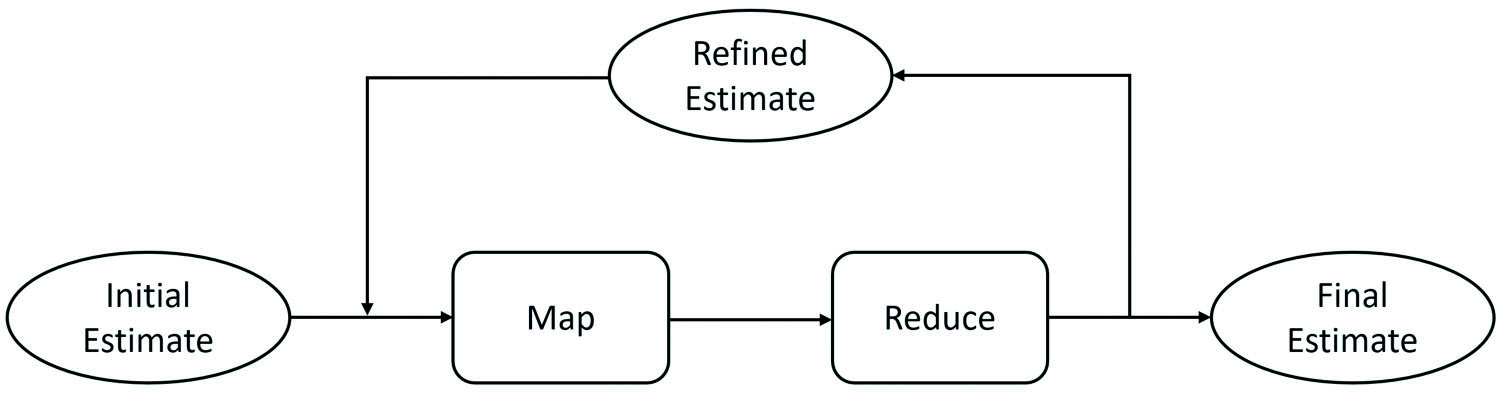
\includegraphics[scale=1]{images-cmyk/iterative-map-reduce-rev}
    \end{center}
    \caption{Iterative map reduce operation.}
    \label{iterative-map-reduce}
\end{figure}

\section{Summary}

Some problems are too large to solve on a single, conventional machine.
That leaves two options.
Get a large machine (a supercomputer, for example),
or break the problem down into many tasks and
perform each task on a separate computer.
The first approach,
\index{scaling!vertical}\index{vertical scaling}vertical scaling,
is limited by the size and speed of the most powerful computer available.
In addition, it is difficult to use in practice because as the problem grows,
several scaling steps may be necessary,
and each step requires an expensive migration to a more capable computer.
If we were trying to use vertical scaling to deal with the massive,
rapid increases in the volume of traffic on websites
like those of Google and Amazon,
we might need an upgrade every few days,
which would be impossible with vertical scaling.

An alternate approach,
\index{scaling!horizontal}\index{horizontal scaling}horizontal scaling,
offers the promise of virtually unlimited
scalability and incremental increase
in the cost of the solution as the problem size grows.
However, it is much more difficult
to write programs that are split across multiple machines,
and this solution works only
for big computations that can be carried out
in the form of many smaller computations.
Such problems usually involve a lot of data,
and the data needs to be in clumps
that can be processed independently.

\index{reduce, map}\index{MapReduce}MapReduce
is a framework related
to the equation-based software model that facilitates writing
programs that can be distributed across a large number of computers.
MapReduce programs are organized around two operations.
The map operation applies to each of the input values, and
it generates an intermediate result.
The intermediate results are subsequently combined using the reduce operation.
If the results generated by the reduce operation are in the same format
as the input to the map operation, multiple MapReduce passes can be performed.
This is useful in programs that estimate optimal results by refining an initial estimate,
such as programs that find clusters in a large data set.

%%% Local Variables:
%%% mode: latex
%%% TeX-master: "book"
%%% End:


\chapter{Generating Art with Computers}
\label{ch:art-computers}

This book has explored deep connections between logic
and computing, including the use of equations and logic to
write and analyze computer programs. In this chapter we're going
to turn our attention to artistic creativity. Can logic and
equations be useful in creating works of art?

\section{Representing Images in a Computer}

To create visual art with a computer, we need some way to
represent images in computers. How does a computer
store a picture?
The answer, it turns out, is surprisingly pedestrian. Ignoring
color for now, you can think of a computer display, such as the
screen on your computer or phone, as a collection of millions
of tiny dots arranged in a rectangular \index{grid, image}grid with a fixed number
of rows and columns. Different displays have different dimensions.
For reference, let's say there are $M$ rows and $N$ columns
in the grid.
Each dot is called a \index{pixel}\emph{pixel}, a term in common use now
that at one time was short for \index{picture}``picture element.''

The computer we are using right now has
a $1440\times900$ display: 900 rows and 1440 columns.
Continuing to ignore color for the moment, each pixel can
be either emitting light (turned on) or not emitting light
(turned off), so a picture in a computer can be represented
by specifying which pixels are ``on'' and which
are ``off.'' A straightforward way to do this is to use a list of
numbers in which each number corresponds to a pixel. Even better,
we can use a list of rows, each of which is list of $N$
0/1 elements (one for each pixel in the row).
The off/on status of the pixels in the row would
match the 0/1 elements in the list,
and there would be $M$ such lists, one for each row on the display.
This list of lists forms a kind of \index{matrix}matrix.

Figure~\ref{fig:glider-in-images} illustrates
this idea with a $4\times4$ grid of squares
representing a $4\times4$ section of pixels in a computer display.
The pixel in row $i$ and column $j$ is ``on''
(indicated in the figure by a black square in the diagram)
when the $j^\text{th}$
entry in the $i^\text{th}$ list is a 1.
When the entry is a 0, the pixel is ``off'' (indicate by white square).

\begin{figure}
\begin{center}
\begin{minipage}{3cm}
\begin{verbatim}
 [[0 1 0 0]
  [0 0 1 0]
  [1 1 1 0]
  [0 0 0 0]]
\end{verbatim}
\end{minipage}%
\begin{minipage}{3cm}
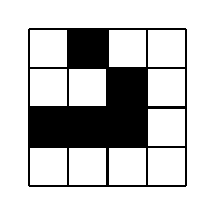
\begin{tikzpicture}[thick, scale=0.5]
\draw (0,0) grid (4,4);
\foreach \c in {(0,1), (1,1), (2,1), (2,2), (1,3)}
    \fill \c + (1, 1) rectangle \c;
\end{tikzpicture}
\end{minipage}
\end{center}
\caption{A Picture Encoded as a Matrix of Pixels}
\label{fig:glider-in-images}
\end{figure}

Using lists to represent \index{image}images is an important concept.
The first chapter of the book talked about boundaries
and interfaces between software and hardware, and these ideas are
well illustrated in this representation of images.
Lists are a well-studied notion and have played a central
role throughout the book.
You probably have a solid grasp of lists at this point.
Now we are using them to represent pictures, which are
physical entities in the real world.
From the software perspective,
generating an image amounts to generating a list of numbers.
It is up to the hardware to interpret the list of numbers
as an image and display it.
We have used equations to generate lists in many contexts,
and these ideas are directly applicable in this new context.

This kind of \index{layering}layering is a common strategy for dealing
with complex problems in computer science.
Each layer in the solution provides a service
to the layers next to it. In this example,
the software layer generates lists of zeros and ones
for the hardware layer, and
the hardware layer turns lists of zeros and ones into physical images.
Both layers represent images, but in different forms.
The software generates an abstraction of an image
in the form of zeros and ones,
and the hardware layer turns that abstraction into an
image on a screen. That is, the hardware builds a
concrete version of the abstraction specified by software.
So far in this example there are only two layers,
but in complex systems, there can be dozens of layers.

So far, so good, with \index{black-and-white}\index{image!black-and-white}black-and-white images,
but what about \index{color}color \index{image!color}images?
The \index{eye, human}human eye perceives
color using specialized cells, called \emph{cones}, in the central
part of the retina. There are three types of cones, each one sensitive
to a different range of colors. There is some overlap in the range
of colors that each type of cone can detect, but it is mostly accurate
to think in terms of cones that are sensitive to shades of red, green,
and blue.

So, color images can be created by using three dots on a screen
for each \index{pixel!color}\index{color!pixel}pixel,
one for red, one for green, and one for blue.
If the red dot in a pixel is on, and the green and blue dots
are off, the pixel looks red. Other colors come from combinations
of red, green, and blue dots.
The following list represents the first row of pixels
in the black-and-white image shown in
Figure \ref{fig:glider-in-images}.
\begin{quote}
    \textsf{[0 1 0 0]}
\end{quote}
In a color image, the row of pixels could be represented by
a list of three-element lists.
\begin{quote}
    \textsf{[[0 0 0] [1 0 0] [0 0 0] [0 0 0]]}
\end{quote}
In this representation, colors are specified as triples of 0/1 values
specifying the off/on status of the color dots in the corresponding pixel.
The first element of the triple is for the red dot, the second
for the green dot, the third for the blue dot.
That is the conventional order:
\index{red-green-blue}red-green-blue (\index{RGB}RGB).
In this scheme, \textsf{[1 0 0]} represents pure red,
so the list, as shown, represents a red dot in the second pixel of the row.

With this convention, there would be eight possible \index{color!eight}colors because
each element in the triple can be either zero or one,
which leads to $2^3$ (that is, $8$) combinations:
black \textsf{[0 0 0]},
white \textsf{[1 1 1]},
red \textsf{[1 0 0]},
green \textsf{[0 1 0]},
blue \textsf{[0 0 1]},
cyan \textsf{[0 1 1]},
magenta \textsf{[1 0 1]},
and
yellow \textsf{[1 1 0]}.
That might be an improvement over black-and-white,
but it's a crude representation of color
compared to the colors the eye can perceive.

Getting more colors requires a more subtle blending of
red, green, and blue. For example, a pixel with red and green
on and blue off will appear to be yellow,
but by using a range of \index{color!intensity}color intensities,
not just on and off, a blend of red and green can produce other
colors, such as orange. The human eye can detect more than 256 shades of
each color, but 256 shades are enough to produce realistic color.
So, it is common to represent color intensity as a number
from 0 to 255. Using this scheme, the list \textsf{[255 140 0]} produces
a dark shade of \index{orange}orange.

In principle, a matrix of \index{red-green-blue}red-green-blue
intensities is
enough to create images, even colorful images.
However, additional layers between the software and hardware
layers can be helpful. Imagine, for example, an operator called \textsf{line}
that paints a line on an image. This operator would figure out
which pixels are on the line and build a matrix with
the appropriate triple for the chosen color at each of those pixels.
\begin{quote}
    \textsf{(line} $image$ $x_1$ $y_1$ $x_2$ $y_2$ $color$\textsf{)}
\end{quote}
The $image$ operand is a matrix of pixels (red-green-blue triples)
representing an image, the $x$ and $y$ values
specify the row/column coordinates of the endpoints of the line,
and $color$ is a triple of red-green-blue color intensities.
The operator delivers a new matrix of color intensities
like the $image$ operand, but with the specified color
at each pixel on the line.

\begin{aside}
Drawing a \index{line!draw}line from one point to another on a grid of points is tricky.
There are many subtle cases to consider, and
if you don't make good choices, the result does not look
like a line at all. If the starting point has
coordinates $(1,1)$ and the end point $(10,10)$,
then the line consists of the points $(1,1)$,
$(2,2)$, $(3,3)$, and so on up to $(10,10)$.
No problem.

However, if the end point is $(2,10)$ instead of $(10,10)$,
then choosing the right points for the line is more difficult.
Sketch a $10\times10$ grid and try drawing a \index{image!line}line
from  $(1,1)$ to  $(2,10)$.
This is an extreme case, but many lines lead to similar issues.
Geometry on a grid,
\index{digital geometry}\index{geometry, digital}digital geometry,
presents a lot of problems like this one that are hard to solve.

Another problem is speed. In many graphics applications, the
computer needs to draw millions or billions of lines per second,
so speed is important.
In the 1960s, the computer scientist
\index{Bresenham, Jack}Jack Bresenham invented
a fast way to compute the list of grid points closest to the line
between any two given endpoints.
Most of the line-drawing in digital images, still today,
makes use of some version of the Bresenham algorithm.
\caption{Bresenham Line-Drawing Algorithm}
\label{aside:Bresenham}
\end{aside}

We're sure you can think of many other useful operators in
the same vein as the operator \textsf{line}. Operators to draw
triangles, squares, rectangles, polygons, circles,
ellipses, and the like. The important thing to realize is that all of
these operators work on an image represented as a matrix of
color intensities.
The operators add to the system a layer that understands
basic geometric shapes on top of the layer that represents an image
as a matrix of pixels.

Operators that create shapes are not the whole story.
Operators of another kind blur \index{image!blur}images in useful ways.
For example, suppose that an image has a
very dark line on a bright background. This creates a
sharp boundary between the line and the background, but it can be
smoothed out by averaging the colors of neighboring pixels.
The bright pixels on one side of the boundary become a little darker,
and the dark pixels on the other side become a little lighter,
resulting in a more subtle boundary. This is the basic idea behind
operators that manipulate images at the level
of individual pixels and their neighbors. Image-processing operators
of this kind form a class of  known as \index{filter}\emph{image filters}.
There are a lot of filters in image
processing software, and they provide another abstraction layer
that facilitates creating representations of images with software.

\section{Generating Images Randomly}

One way to generate artistic images is to insert a layer of
randomness on top of the layers that create geometric shapes.
An artist may layer \index{painting}paints on a canvas
with a brush that has a certain texture, and the brush strokes
will create a complex pattern that is more than just a line.
Figure~\ref{fig:line-art} shows a pair of images.
One is a straight line
and the other shows how adding a lot of nearby, short lines in
more-or-less random orientations
creates an image similar to a line, but with more texture,
like a brush stroke, perhaps.
Similar operations can produce
other geometric shapes with a degree of randomness,
such as in noisy rectangles or circles that are
mostly, but not exactly, round.

\begin{figure}
\begin{center}
\begin{tabular}{ll}
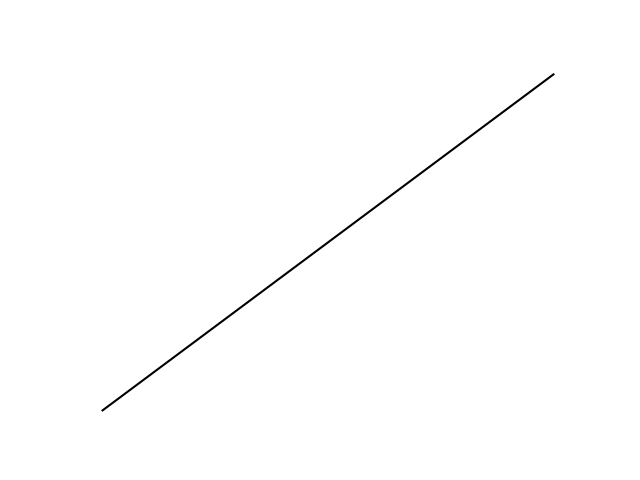
\includegraphics[scale=0.3]{images/straight-line.png} &
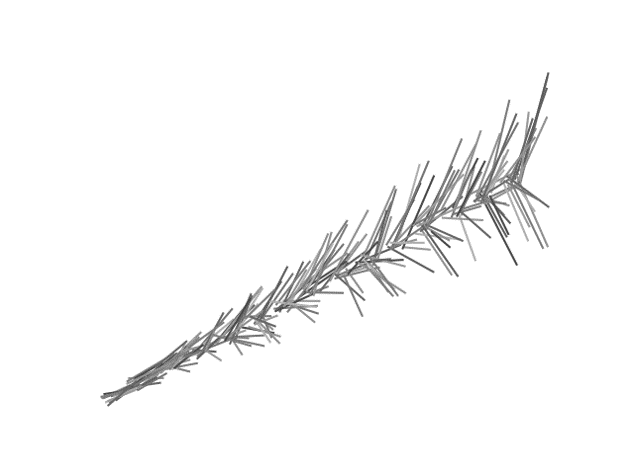
\includegraphics[scale=0.3]{images/random-line-art.png} \\
\end{tabular}
\end{center}
\caption{Straight Line vs.~a Line Made Up of Random Segments}
\label{fig:line-art}
\end{figure}

But what do we mean by \index{random}random?
None of the digital circuits
that we have studied exhibit random behavior.
Instead, they conform to precise equations and deliver the same
results every time they are supplied with the same data.
The following sequence of numbers appears to be random.
$$0, 1, 5, 3, 4, 8, 6, 7, 2, 0$$
However, it is not random. It is produced by an
operator $r$ defined by the following equations,
which are presented in both traditional, algebraic form
and in ACL2 notation.\footnote{You can ignore the ACL2
if you have not yet studied the chapters that introduce it.
The ACL2 versions of the equations don't add any information
necessary to understanding the concepts presented in this chapter.}

\begin{center}
\begin{tabular}{ll}
$r(n+1) = (4\cdot r(n) + 1)$ $mod$ $9$ & \{r1\}\\
$r(0) = 0$                        & \{r0\}\\
\end{tabular}
\end{center}

\begin{Verbatim}
(defun r (n)
 (if (zp n)
     0                                 ; {r0}
     (mod (+ (* 4 (r (- n 1))) 1) 9))) ; {r1}
\end{Verbatim}

As you can easily check if you
recall that ($x$ $mod$ $d$) is the remainder in
the division $x \div d$
(Aside~\ref{third-grade-division}, page \pageref{third-grade-division}),
$r(0) = 0$, $r(1) = 1$, $r(2
) = 5$, $r(3) = 3$,
and so on.
So, $r$ is an operator that appears to produce random
numbers, but the process is completely deterministic.
The sequences produced by such operators
are called \emph{pseudo-random}
\index{random!pseudo}\index{pseudo-random}\index{sequence!pseudo-random}sequences,
and they provide a way to introduce an aspect of randomness into images.

There are many ways to produce pseudo-random sequences.
It is a well-studied problem with a long history and lots
fascinating ramifications. It happens that the operator
$r$ belongs to the most commonly used
family of pseudo-random number generators: the
\index{random!number generator}\index{linear congruential}linear congruential generators.
A linear congruential generator has a \emph{seed}, which is
the value it delivers as the first number in the sequence.
It also has a \emph{multiplier}, an \emph{increment}, and a \emph{modulus}.
The $(n+1)^\text{th}$ number in the sequence
is produced by multiplying the $n^\text{th}$ number by
the multiplier, adding the increment, and delivering
the remainder when that sum is divided by the modulus.
The multiplier, increment, and modulus for the operator $r$
are $4$, $1$, and $9$, respectively.
One of the effects of the modulus is to keep the numbers
within a certain range, which is the range $0$, $1$, \dots $8$ in
the case of the operator $r$.

It is common to define pseudo-random operators like $r$ in
manner that, to compute a number in the pseudo-random sequence,
requires the previous value in the sequence as the operand.
This is different from the definition of $r$, where the
operand is the index of the number in the sequence: $r(n)$ is the
$n^\text{th}$ number in the sequence.
It turns out that more common method,
in which each invocation
supplies the value delivered by the previous invocation as
the operand, is much faster than
the operator $r$
because the definition is no longer inductive,
as shown in the following definition of the operator
$rs$.\footnote{Again, you won't miss the point
if you ignore the ACL2 version of the equations.}

\begin{center}
\begin{tabular}{ll}
$rs(s) = (4s + 1)$ $mod$ $9$ & \{rs\}\\
\end{tabular}
\end{center}

\begin{Verbatim}
(defun rs (s)
  (mod (+ (* 4 s) 1) 9))  ; {rs}
\end{Verbatim}

Because the modulus is 9 in the definitions of the operators
$r$ and $rs$, they always deliver a natural number between 0 and 8.
All linear congruential random number generators
have a fixed range (although it is usually a much bigger range than 0 to 8),
so they always deliver
a natural number between 0 and $D-1$, where $D$ is the modulus.\footnote{It
is often more convenient to work with random numbers between $0$ and $1$
instead of integers between zero and the modulus.
That is easily accomplished by dividing the generated number
by the modulus.}

\begin{figure}
\begin{center}
\begin{tabular}{lll}
$ragged(image, x_1, y_1, x_2, y_2, seed) =$  &&\{rg1\}\\
\hspace*{8mm}$ragged(line(image, x_1, y_1, rx, ry, black), x, y, x_2, y_2, s)$ & if $x_1 < x_2$ &\\
\hspace*{4mm}where &&\\
\hspace*{4mm}$s = rs(seed)$    &&\\
\hspace*{4mm}$jostle = s/9 - 1/2$    &&\\
\hspace*{4mm}$slope = (y_2 - y_1)/(x_2 - x_1)$    &&\\
\hspace*{4mm}$rx = x_1 + 10$     &&\\
\hspace*{4mm}$ry = y_1 + round(10\cdot(slope + jostle))$ &&\\
\hspace*{4mm}$x = x_1 + 1$     &&\\
\hspace*{4mm}$y = y_1 + round(slope)$ &&\\
\hspace*{4mm}$b =$ \textsf{[0 0 0]} &&\\
$ragged(image, x_1, x_2, y_1, y_2, seed) = image$ & if $x_1 \geq x_2$ &\{rg0\}\\
\end{tabular}

\begin{Verbatim}
(defun ragged (image x1 y1 x2 y2 seed)
 (if (< x1 x2)
     (let* ((s (rs seed))
            (jostle (- (/ s 9) 1/2))
            (slope (/ (- y2 y2) (- x2 x1)))
            (rx (+ x1 10))
            (ry (+ y1 (round(* 10 (+ slope jostle)))))
            (x (+ x1 1))
            (y (+ y1 (round slope)))
            (black (list 0 0 0)))
       (ragged (line image x1 y1 rx ry black) x y x2 y2 s) ; {rg1}
     image))                                               ; {rg0}
\end{Verbatim}
\end{center}
\caption{Operator to Draw a Ragged Line Using Random Numbers}
\label{fig:ragged-defun}
\end{figure}

The operator defined by the equations in
Figure~\ref{fig:ragged-defun} (page \pageref{fig:ragged-defun})
draws a \index{ragged line}ragged \index{line!ragged}line
by drawing short line segments at randomized angles
from starting points along the line from $(x_1,y_1)$ to $(x_2,y_2)$.
The starting points of the short line segments are
spaced one unit apart in the $x$ direction.
The $x$ coordinate of the endpoint of a short segment
is ten more than $x$ coordinate of the starting point
(that is, $x_1 + 10$).
The $y$ coordinate of that endpoint is computed
by moving in the general direction of the target
$(x_2,y_2)$, but with the direction
randomly adjusted by a small amount.
The adjustment is made by adding a random number between
$-1/2$ and $1/2$ to the \emph{slope},
$(y_2 - y_1)/(x_2 - x_1)$, then multiplying that
number by ten (the difference between the
starting $x$ coordinates of the endpoint
and starting point of the short segment,
in the usual manner of computing coordinates
along a straight line, algebraically).

The slope used in the computation is a ratio of
two integers, but (usually) is not an integer.
Since grid-points have integer coordinates,
the numbers computed using the slope
are rounded to the nearest integer by
an operator called \textsf{round}. That way,
all of the coordinates supplied as
operands to the \textsf{line} operator
and the operator \textsf{ragged} are pairs of
integers representing grid points.
The \textsf{line} operator won't draw any lines
that extend outside the boundaries of
the image, so if any of the computed
coordinates are out of range,
the line segments that are drawn will
be truncated at the image boundary.

The short segments are drawn in this way along
the line between $(x_1,y_1)$ and $(x_2,y_2)$,
with starting points whose $x$ coordinates
take all the integer values between $x_1$ and $x_2$.
This makes the starting points close together along
the points on the grid that are closest to the
line between $(x_1,y_1)$ and $(x_2,y_2)$.
The effect is a ragged line that looks more organic
than a simple, straight line.
This is the idea behind the line
in Figure~\ref{fig:line-art} (page \pageref{fig:line-art}).

In the inductive equation \{rg1\} in the definition of the operator \textsf{ragged},
the \emph{seed} operand is supplied to the pseudo-random
number generator $rs$, and that operator uses it to produce
a number $s$ between 0 and 8. That number is supplied as the last
operand in the invocation of \textsf{ragged} in the inductive equation \{rg1\}
(so it can be used to generate the next random number),
and it is also used to \index{jostle}jostle
the slope of the short line segment drawn by the operator \textsf{line}.
The operator \textsf{line} produces a new image,
which is the first operand in the invocation of \textsf{ragged} in equation \{rg1\}.
In this way, the image accumulates the line segments that the operator \textsf{line}
draws at each stage.

\section{Generating Purposeful Images}

Random images can be nice to look at, but should they be called art?
Can a computer program produce real works of art?
That is a philosophical question with lots of answers.
But, regardless of how you might answer the question,
there are a handful of programs that, it has been reasonably argued,
are artists. Let's look at one of them.

The program \index{AARON software}AARON,
written over a span of decades by artist \index{Cohen, Harold}Harold Cohen,
was designed in part as an exploration of artmaking. Cohen's
initial goal was to determine when a group of abstract marks can
be recognized as a coherent image. The earliest versions of his program
could do very little, and those early versions knew very little about art.
Those versions knew the difference between a figure and the ground, and also
the difference between an open figure and a closed figure, but
not much more.

What made the early versions of AARON effective was a layer that
stood on top of the low-level drawing layer. This layer was essentially
a list, but instead of pixel colors, this list contained graphical objects
and their locations. Adding a new figure to the canvas was accomplished
by adding a new object to the master list. The real breakthrough was
that this list could be examined during the process of adding
a new figure, so AARON could effectively reflect on the work it had
done earlier, then proceed with additional work.
This allowed the software to make decisions based on
artistic principles, such as balance and proportion.
This breakthrough proved so successful
that it carried over into all subsequent versions of AARON.

An obvious way to enhance AARON would have been to add more graphical
primitives, such as new figures that it could draw. But
the next step in AARON's evolution was something more profound. What
Cohen did was to enhance the program so that it could ``scribble'' around
``core figures.'' This idea came from observing the way children
scribble on paper, and in particular the key moment when the children
seemed to realize that a figure they scribbled actually represented a
realistic object in some sense. From AARON's perspective, the main improvement
was a two-step strategy where \index{core figures}core figures
were placed in a virtual world,
and then the picture was allowed to evolve by tracing a kind of path
around the core figures.
This strategy resulted in paintings with much more complexity
and a sense of realism, in that the end product showed realistic-looking
objects that seemed to be inspired by the real world. Certainly, if a
human artist had drawn these shapes, they would have been considered to be
reflections of the real world.

From this point on, AARON became more and more \emph{representational} in
the works it produced. This came from three main sources of improvement. The first
was a database of core figures that combined to represent visually some
objects from the real world. Each core figure was represented as a list of
key points that provided essentially an outline, and the figures were connected
in space and orientation.
For example, a plant could be represented by
a trunk, some branches, and some leaves. Each of those may be a core figure,
and the figures would be related to each other geometrically, which is to say
that the branches are connected to the trunk, and the leaves to the branches.
This basic strategy worked to model even complex objects, such as a basic human
form and a recognizable image of the Statue of Liberty.

The second improvement was a series of algorithms that could create reasonable
objects made up of core figures. It is not feasible to model all possible
objects using core figures. So, Cohen wrote some algorithms that allowed AARON to
imagine \index{quasi-plants}\index{plants, quasi}plants,
or as he called them \emph{quasi-plants}. It probably won't surprise
you to learn that these algorithms made extensive use of pseudo-random numbers.
At this point, AARON's paintings featured recognizable human shapes
in an environment that included many plant-like shapes.

Finally, the third improvement was the development of a set of rules that
let AARON render an image from a world described by core figures. Essentially,
these rules amount to expertise in drawing. For example, the core figures occupy
a space in three dimensions, and the rules determine how AARON is to deal with
geometric problems such as perspective and occlusion. That is, figures farther
away must appear smaller in the final image, and a core figure near the front may
partially hide a figure that is farther away. AARON is truly becoming an expert
painter, which is one aspect of being an artist.

AARON's paintings from this time represent a high point in its work, and they
have been exhibited in museums.
Nevertheless, there was a hidden limitation, in that the core figures
used to build AARON's model of the world were two-dimensional. The figures could be
placed in a three-dimensional world, but the realism in AARON's work was partially
due to the limitations in the scale of its paintings. Cohen wanted to create larger
and more complex paintings, and he felt that this increase in scale would require a
more detailed model of the real world in AARON's data structures.

So, Cohen embarked on a new modeling phase with more detailed and fully
three-dimensional models of the objects that AARON would draw, such as the human
body. These models were made of groups of three-dimensional points that were
related to other similar groups, in a way that is clearly derived from the earlier
core figures. In a tradition dating back to da Vinci and Michelangelo, the models
for the human body were taken directly from anatomical studies. This shift
created many complications because AARON's model was now three-dimensional,
so it had to create two-dimensional projections of core images before rendering a
painting.

The complications are significant, and you might find it interesting to pursue
it further by reading Cohen's own description
of his work or \index{McCorduck, Pamela}Pamela McCorduck's
very readable account of AARON's evolution as an
artist---even to the point of mixing its own pigments and painting its own artworks
on a physical canvas.

What we want to leave you with is an appreciation that
simple principles can indeed lead to complex behavior.
AARON's knowledge of the real world is encoded as a set of points,
and its expertise in drawing is encoded as a set of rules.
This is analogous to the way we used equations and logic to write programs,
create models of digital circuits, and reason about properties of those abstractions.
AARON is an impressive program, and it can be plausibly argued that it exhibits
artistic creativity. But at its core, it is
composed of simple principles that, taken as a whole, capture a way of painting.

%%% Local Variables:
%%% mode: latex
%%% TeX-master: "book"
%%% End:


\backmatter

%clear, phantom, addcontents puts Index in ToC at level of Part I, II, ...
\cleardoublepage
\phantomsection
\addcontentsline{toc}{part}{Index}
\printindex

\cleardoublepage
\pagestyle{empty}
\null\vfil

\begin{adjustwidth}{1in}{1in}
\begin{center}
{\Large\textsf{Colophon}}
\end{center}
\begin{center}
This manual was typeset using the \LaTeX\ typesetting system
created by Leslie Lamport and the memoir class.
The body text is set 10/12pt on a
33pc measure with Palatino designed by Hermann Zapf, which includes
italics and small caps. Other fonts include
Sans, Slanted and Typewriter from Donald Knuth's
Computer Modern family.

\end{center}

\end{adjustwidth}

\vfil

\end{document}

